%%%%%%%%%%%%%%
%% Run LaTeX on this file several times to get Table of Contents,
%% cross-references, and citations.

%% If you have font problems, you may edit the w-bookps.sty file
%% to customize the font names to match those on your system.

%% w-bksamp.tex. Current Version: Feb 16, 2012
%%%%%%%%%%%%%%%%%%%%%%%%%%%%%%%%%%%%%%%%%%%%%%%%%%%%%%%%%%%%%%%%
%
%  Sample file for
%  Wiley Book Style, Design No.: SD 001B, 7x10
%  Wiley Book Style, Design No.: SD 004B, 6x9
%
%
%  Prepared by Amy Hendrickson, TeXnology Inc.
%  http://www.texnology.com
%%%%%%%%%%%%%%%%%%%%%%%%%%%%%%%%%%%%%%%%%%%%%%%%%%%%%%%%%%%%%%%%

%%%%%%%%%%%%%
% 7x10
%\documentclass{wileySev}

% 6x9
\documentclass{wileySix}

\usepackage{graphicx}
\usepackage{listings}
\usepackage{float}
\usepackage[urlcolor=blue, colorlinks=true]{hyperref}
\usepackage{textcomp}
\usepackage{gensymb}
\usepackage{color}
 
\definecolor{codegreen}{rgb}{0,0.6,0}
\definecolor{codegray}{rgb}{0.5,0.5,0.5}
\definecolor{codepurple}{rgb}{0.58,0,0.82}
\definecolor{backcolour}{rgb}{0.95,0.95,0.92}
 
\lstdefinestyle{mystyle}{
    backgroundcolor=\color{backcolour},   
    commentstyle=\color{codegreen},
    keywordstyle=\color{magenta},
    numberstyle=\tiny\color{codegray},
    stringstyle=\color{codepurple},
    basicstyle=\footnotesize,
    breakatwhitespace=false,         
    breaklines=true,                 
    captionpos=b,                    
    keepspaces=true,                 
    numbers=left,                    
    numbersep=5pt,                  
    showspaces=false,                
    showstringspaces=false,
    showtabs=false,                  
    tabsize=2,
    language=sh
}
 
\lstset{style=mystyle}

%%%%%%%
%% for times math: However, this package disables bold math (!)
%% \mathbf{x} will still work, but you will not have bold math
%% in section heads or chapter titles. If you don't use math
%% in those environments, mathptmx might be a good choice.

% \usepackage{mathptmx}

% For PostScript text
\usepackage{w-bookps}

%%%%%%%%%%%%%%%%%%%%%%%%%%%%%%%%%%%%%%%%%%%%%%%%%%%%%%%%%%%%%%%%
%% Other packages you might want to use:

% for chapter bibliography made with BibTeX
% \usepackage{chapterbib}

% for multiple indices
% \usepackage{multind}

% for answers to problems
% \usepackage{answers}

%%%%%%%%%%%%%%%%%%%%%%%%%%%%%%
%% Change options here if you want:
%%
%% How many levels of section head would you like numbered?
%% 0= no section numbers, 1= section, 2= subsection, 3= subsubsection
%%==>>
\setcounter{secnumdepth}{3}

%% How many levels of section head would you like to appear in the
%% Table of Contents?
%% 0= chapter titles, 1= section titles, 2= subsection titles, 
%% 3= subsubsection titles.
%%==>>
\setcounter{tocdepth}{2}

%% Cropmarks? good for final page makeup
%% \docropmarks

%%%%%%%%%%%%%%%%%%%%%%%%%%%%%%
%
% DRAFT
%
% Uncomment to get double spacing between lines, current date and time
% printed at bottom of page.
% \draft
% (If you want to keep tables from becoming double spaced also uncomment
% this):
% \renewcommand{\arraystretch}{0.6}
%%%%%%%%%%%%%%%%%%%%%%%%%%%%%%

%%%%%%% Demo of section head containing sample macro:
%% To get a macro to expand correctly in a section head, with upper and
%% lower case math, put the definition and set the box 
%% before \begin{document}, so that when it appears in the 
%% table of contents it will also work:

\newcommand{\VT}[1]{\ensuremath{{V_{T#1}}}}

%% use a box to expand the macro before we put it into the section head:

\newbox\sectsavebox
\setbox\sectsavebox=\hbox{\boldmath\VT{xyz}}

%%%%%%%%%%%%%%%%% End Demo


\begin{document}


\booktitle{Cerdas Menguasai Git}
\subtitle{Dalam 24 Jam}

\authors{Rolly M. Awangga\\
\affil{Informatics Research Center}
%Floyd J. Fowler, Jr.\\
%\affil{University of New Mexico}
}

\offprintinfo{Cerdas Menguasai Git, First Edition}{Rolly M. Awangga}

%% Can use \\ if title, and edition are too wide, ie,
%% \offprintinfo{Survey Methodology,\\ Second Edition}{Robert M. Groves}

%%%%%%%%%%%%%%%%%%%%%%%%%%%%%%
%% 
\halftitlepage

\titlepage


\begin{copyrightpage}{2019}
%Survey Methodology / Robert M. Groves . . . [et al.].
%\       p. cm.---(Wiley series in survey methodology)
%\    ``Wiley-Interscience."
%\    Includes bibliographical references and index.
%\    ISBN 0-471-48348-6 (pbk.)
%\    1. Surveys---Methodology.  2. Social 
%\  sciences---Research---Statistical methods.  I. Groves, Robert M.  II. %
%Series.\\
%
%HA31.2.S873 2007
%001.4'33---dc22                                             2004044064
\end{copyrightpage}

\dedication{`Jika Kamu tidak dapat menahan lelahnya belajar, 
Maka kamu harus sanggup menahan perihnya Kebodohan.'
~Imam Syafi'i~}

\begin{contributors}
\name{Rolly Maulana Awangga,} Informatics Research Center., Politeknik Pos Indonesia, Bandung,
Indonesia



\end{contributors}

\contentsinbrief
\tableofcontents
%\listoffigures
%\listoftables
%\lstlistoflistings


\begin{foreword}
Sepatah kata dari Kaprodi, Kabag Kemahasiswaan dan Mahasiswa
\end{foreword}

\begin{preface}
Buku ini diciptakan bagi yang awam dengan git sekalipun.

\prefaceauthor{R. M. Awangga}
\where{Bandung, Jawa Barat\\
Februari, 2019}
\end{preface}


\begin{acknowledgments}
Terima kasih atas semua masukan dari para mahasiswa agar bisa membuat buku ini 
lebih baik dan lebih mudah dimengerti.

Terima kasih ini juga ditujukan khusus untuk team IRC yang 
telah fokus untuk belajar dan memahami bagaimana buku ini mendampingi proses 
Intership.
\authorinitials{R. M. A.}
\end{acknowledgments}

\begin{acronyms}
\acro{ACGIH}{American Conference of Governmental Industrial Hygienists}
\acro{AEC}{Atomic Energy Commission}
\acro{OSHA}{Occupational Health and Safety Commission}
\acro{SAMA}{Scientific Apparatus Makers Association}
\end{acronyms}

\begin{glossary}
\term{git}Merupakan manajemen sumber kode yang dibuat oleh linus torvald.

\term{bash}Merupakan bahasa sistem operasi berbasiskan *NIX.

\term{linux}Sistem operasi berbasis sumber kode terbuka yang dibuat oleh Linus Torvald
\end{glossary}

\begin{symbols}
\term{A}Amplitude

\term{\hbox{\&}}Propositional logic symbol 

\term{a}Filter Coefficient

\bigskip

\term{\mathcal{B}}Number of Beats
\end{symbols}

\begin{introduction}

%% optional, but if you want to list author:

\introauthor{Rolly Maulana Awangga, S.T., M.T.}
{Informatics Research Center\\
Bandung, Jawa Barat, Indonesia}

Pada era disruptif  \index{disruptif}\index{disruptif!modern} 
saat ini. git merupakan sebuah kebutuhan dalam sebuah organisasi pengembangan perangkat lunak.
Buku ini diharapkan bisa menjadi penghantar para programmer, analis, IT Operation dan Project Manajer.
Dalam melakukan implementasi git pada diri dan organisasinya.

Rumusnya cuman sebagai contoh aja biar keren\cite{awangga2018sampeu}.

\begin{equation}
ABC {\cal DEF} \alpha\beta\Gamma\Delta\sum^{abc}_{def}
\end{equation}

\end{introduction}

%%%%%%%%%%%%%%%%%%Isi Buku_

\chapter{Chapter 1}
%\section{1174006 - Kadek Diva Krishna Murti}

\subsection{Teori}
\subsubsection{Definisi Kecerdasan Buatan}
\hfill\break
Kecerdasan buatan atau artificial intelligence (AI) menurut beberapa pakar adalah sebagai berikut:
\begin{enumerate}
	\item Schalkoff (1990): AI adalah bidang studi yang mencoba meniru dan menerangkan perilaku cerdas yang dilakukan oleh manusia dalam bentuk proses komputasi.
	\item Rich dan Knight (1991): AI adalah studi tentang cara membuat komputer melakukan sesuatu yang sampai saat ini orang dapat melakukannya lebih baik.
	\item Luger dan Stubblefield (1993): AI adalah cabang ilmu komputer yang berhubungan dengan otomasi perilaku yang cerdas.
	\item Keen dan Haag (1996): AI adalah cabang ilmu komputer yang berkaitan dengan pemodelan, penangkapan, dan penyimpanan kecerdasan manusia ke dalam sebuah sistem teknologi informasi sehingga sistem tersebut nantinya dapat memfasilitasi dalam melakukan pengambilan keputusan yang biasanya dilakukan oleh manusia.
\end{enumerate}
\noindent
Jadi dapat disimpulkan kecerdasan buatan atau artificial intelligence (AI) merupakan salah satu bagian ilmu komputer yang membuat mesin (komputer) dapat melakukan pekerjaan seperti dan sebaik yang dilakukan oleh manusia. Seperti yang kita tahu pada awal diciptakannya, komputer hanya difungsikan sebagai alat hitung saja. Namun seiring dengan perkembangan jaman, maka peran komputer semakin mendominasi kehidupan umat manusia. Komputer tidak lagi sekedar digunakan sebagai alat hitungn namun diharapkan untuk dapat diberdayakan untuk mengerjakan segala sesuatu yang bisa dikerjakan oleh manusia.

\subsubsection{Sejarah dan Perkembangan Kercerdasan Buatan}
\hfill\break
Istilah AI pertama kali dikemukakan pada tahun 1956 dikonferensi Darthmouth. Sejak saat itu AI terus dikembangkan sebab berbagai penelitian mengenai teori-teori dan prinsip-prinsipnya juga terus berkembang. Meskipun istilah AI baru muncul tahun 1956, tetapi teori-teori mengarah ke AI sudah muncul sejak tahun 1941. Berikut ini tahapan-tahapan sejarah perkembangan AI:
\begin{enumerate}
	\item Era Komputer Elektronik (1941)
	\hfill\break
	Pada tahun 1941 telah ditemukan alat penyimpanan dan pemrosesan informasi. Penemuan tersebut dinamakan komputer elektronik yang dikembangkan di USA dan Jerman. Komputer pertama ini memerlukan ruangan yang luas dan ruang AC yang terpisah. Saat itu komputer meibatkan konfigurasi ribuan kabel untuk menjalankan suatu program. Hal ini sangat merepotkan bagi para programmer. Pada tahun 1949, berhasil dibuat komputer yang mampu menyimpan program sehingga membuat pekerjaan untuk memasukkan program menjadi lebih mudah. Penemuan ini menjadi dasar pengembangan program yang mengarah ke AI.

	\item Masa Persiapan AI (1943–1956)
	\hfill\break
	Pada tahun 1943, Warren McCulloch dan Walter Pitts mengemukakan tiga hal: pengetahuan fisiologi dasar dan fungsi sel syaraf dalam otak, analisis formal tentang logika proporsi (propositional logic), dan teori komputasi turing. Mereka berhasil membuat suatu model syaraf tiruan (artificial neuron) di mana setiap neuron digambarkan sebagai on dan off. Mereka menunjukkan bahwa setiap fungsi dapat dihitung dengan suatu jaringan sel syaraf dan bahwa semua hubungan logis dapat diimplementasikan dengan struktur jaringan yang sederhana.
	\noindent
	Pada tahun 1950, Norbert Wiener mebuat penelitian mengenai prinsip-prinsip teori feedback. Contoh yang terkenal adalah thermostat. Penemuan ini juga merupakan awal perkembangan AI. Pada tahun 1956, John McCarthy (yang setelah lulus dari Princeton kemudian melanjutkan ke Dartmouth College) meyakinkan Minsky, Claude Shannon dan Nathaniel Rochester untuk membantunya melakukan penelitian dalam bidang Automata, jaringan sel syaraf dan pembelajaran intelejensia. Mereka mengerjakan proyek ini selama dua bulan di Dartmouth. Hasilnya adalah program yang mampu ber-pikir non-numerik dan menyelesaikan masalah pemikiran, yang dinamakan Principia Mathematica. Hal ini menjadikan McCarthy disebut sebagai Father of AI (Bapak AI).

	\item Awal Perkembangan AI (1952–1969)
	\hfill\break
	Pada tahun-tahun pertama pengembangannya, AI mengalami banyak kesuksesan. Diawali dengan kesuksesan Newell dan Simon dengan sebuah program yang disebut General Problem Solver. Program ini dirancang untuk memulai penyelesaian masalah secara manusiawi. Pada tahun 1958, McCarthy di MTT Lab Memo No. 1 mendefinisikan bahasa pemrograman tingkat tinggi yaitu LISP, yang sekarang mendominasi pembuatan program-program AI. Kemudian, McCarthy membuat program yang dinamakan Programs With Common Sense. Di dalam program tersebut, dibuat rancangan untuk menggunakan pengetahuan dalam mencari solusi. Pada tahun 1959, Nathaniel Rochester dari IBM dan mahasiswa-mahasiswanya mengeluarkan program AI Geometry Theorm Prover. Program ini dapat membuktikan suatu teorema menggunakan axioma-axioma yang ada. Pada tahun 1963, program yang dibuat James Slagle mampu menyelesaikan masalah integral tertutup untuk mata kuliah kalkulus. Pada tahun 1968, program analogi buatan Tom Evan menyelesaikan masalah analogi geometris yang ada pada tes IQ.

	\item Perkembangan AI Melambat (1966–1974)
	\hfill\break
	Prediksi Herbert Simon pada tahun 1957 yang menyatakan bahwa AI akan menjadi ilmu pengetahuan yang akan berkembang dengan pesat ternyata meleset. Pada 10 tahun kemudian, perkembangan AI melambat. Hal ini disebabkan adanya 3 kesulitan utama yang dihadapi AI, yaitu:
	\begin{enumerate}
		\item Masalah pertama: program-program AI yang bermunculan hanya mangandung sedikit atau bahkan tidak mengandung sama sekali pengetahuan (knowledge) pada subjeknya. Program-program AI berhasil hanya karena manipulasi sintetis yang sederhana. Sebagai contoh adalah Weizenbaum’s ELIZA program (1965) yang dapat melakukan percakapan serius pada berbagai topik, sebenarnya hanyalah peminjaman dan manipulasi kalimat-kalimat yang diketikkan oleh manusia.
		\item Masalah kedua: banyak masalah yang harus diselesaikan oleh AI. Karena terlalu banyaknya masalah yang berkaitan, maka tidak jarang banyak terjadi kegagalan pada pembuatan program AI.
		\item Masalah ketiga: ada beberapa batasan pada struktur dasar yang digunakan untuk menghasilkan perilaku intelejensia. Sebagai contoh adalah pada tahun 1969 buku Minsky dan Papert Perceptrons membuktikan bahwa program-program perceptrons dapat mempelajari segala sesuatu, tetapi program-program tersebut hanya mempresentasikan sejumlah kecil saja. Sebagai contoh dua masukan perceptrons yang berbeda tidak dapat dilatihkan untuk mengenali kedua masukan yang berbeda tersebut.
	\end{enumerate}

	\item Sistem Berbasis Pengetahuan (1969–1979)
	\hfill\break
	Pengetahuan adalah kekuatan pendukung AI. Hal ini dibuktiikan dengan program yang dibuat oleh Ed Feigenbaum,Bruce Buchanan dan Joshua Lederberg yang membuat program untuk memecahkan masalah struktur molekul dari informasi yang didapatkan dari spectometer massa. Program ini dinamakan Dendral programs yang berfokus pada segi pengetahuan kimia. Dari segi diagnosis media juga sudah ada yang menemukannya, yaitu Saul Amarel dalam proyek computer in biomedicine. Proyek ini diawali dari keinginan untuk mendapatkan diagnosa penyakit berdasarkan pengetahuan yang ada pada mekanisme penyebab proses penyakit.

	\item AI Menjadi Sebuah Industri (1980–1988)
	\hfill\break
	Industrialisasi AI diawali dengan ditemukannya expert system (sistem pakar) yang dinamakan R1 yang mampu mengkonfigurasi sistem-sistem komputer baru. Program tersebut mulai dioperasikan di Digital Equipment Corporation(DEC), McDermott, pada tahun 1982. Pada tahun 1986, program ini telah berhasil menghemat US\$40 juta per tahun. Pada tahun 1988, kelompok AI di DEC menjalankan 40 sistem pakar. Hampir semua perusahaan besar di USA mempunyai divisi AI sendiri yang menggunakan ataupun mempelajari sistem pakar. Booming industri AI ini juga melibatkan perusahaan-perusahaan besar seperti Carnegie Group, Inference, Intellicorp, dan Technoledge yang menawarkan software tools untuk membangun sistem pakar. Perusahaan hardware seperti LISP dan Machines Inc., Texas Instruments, Symbolics, dan Xerox juga turut berperan dalam membangun workstation yang dioptimasi untuk pembangunan program LISP. Sehingga, perusahaan yang sejak tahun 1982 hanya menghasilkan beberapa juta US dolar per tahun meningkat menjadi 2 milyar US dolar per tahun pada tahun 1988.

	\item Kembalinya Jaringan Syaraf Tiruan (1986–Sekarang)
	\hfill\break
	Meskipun bidang ilmu komputer menolak jaringan syaraf tiruan setelah diterbitkannya buku "perceptrons" karangan Minsky dan Papert, tetapi para ilmuan masih mempelajari bidang ilmu tersebut dari sudut pandang yang lain yaitu fisika. Para ahli seperti Hopfield (1982) menggunakan teknik-teknik mekanika statistika untuk menganalisa sifat-sifat penyimpanan dan optimasi pada jaringan syaraf. Para ahli psikollogi, David Rumelhart dan Geoff Hinton, melanjutkan penelitian mengenai model syaraf pada memori. Pada tahun 1985-an sedikitnya empat kelompok riset menemukan kembali algoritma belajar propagasi balik (Back-Propagation Learning). Algoritma ini berhasil diimplementasikan kedalam bidang ilmu komputer dan psikologi.

\end{enumerate}

\subsubsection{Supervised Learning}
\hfill\break
Supervised Learning adalah pembelajaran yang memiliki label di tiap datanya. Label maksudnya adalah tag dari data yang ditambahkan dalam machine learning model. Contohnya gambar kucing di tag "kucing" di tiap masing masing image kucing dan gambar anjing di tag "anjing" di tiap masing gambar anjing. Machine learning kategori dapat berupa clasification ("anjing", "kucing", "beruang", dsb) dan regression ( berat badan, tinggi badan dsb). Supervised learning banyak digunakan dalam memprediksi pola dimana pola tersebut sudah ada contoh data yang lengkap, jadi pola yang terbentuk adalah hasil pembelajaran data lengkap tersebut. Tentunya jika kita memasukan data baru, setelah kita melakukan ETL (Extract Transform Load) maka kita mendapat info feature feature dari sample baru tersebut. Kemudian dari feature feature tersebut di compare dengan pattern clasification dari model yang didapat dari labeled data. Setiap label akan dicompare sampai selesai, dan yang memiliki percentage lebih banyak akan diambil sebagai prediksi akhir.

\begin{figure}[H]
	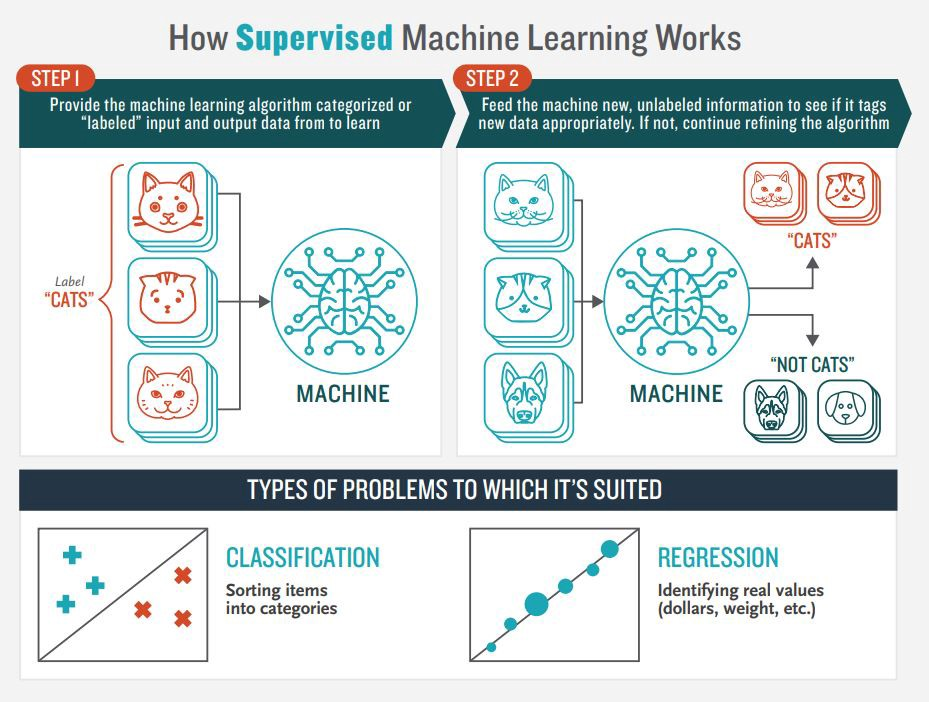
\includegraphics[width=1\textwidth]{figures/1174006/chapter1/supervisedlearning.jpeg}
	\centering
	\caption{Supervised Learning.}
\end{figure}
\noindent
Contoh algoritma yang digunakan pada supervised learning meliputi :
\begin{enumerate}
	\item Clasification (Categorical) and Regression (Numerical)
    \item Logistic Regression
    \item Model Ensemble
	\item Time series
\end{enumerate}

\subsubsection{Klasifikasi}
\hfill\break
Classification adalah tindakan untuk memberikan kelompok pada setiap keadaan. Setiap keadaan berisi sekelompok atribut, salah satunya adalah class attribute. Metode ini butuh untuk menemukan sebuah model yang dapat menjelaskan class attribute itu sebagai fungsi dari input attribute.
\begin{figure}[H]
	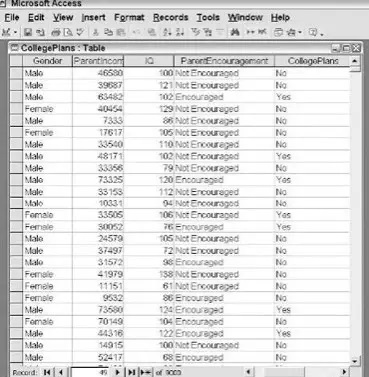
\includegraphics[width=1\textwidth]{figures/1174006/chapter1/clasification.jpg}
	\centering
	\caption{Clasification.}
\end{figure}
\noindent
Class adalah attribute CollegePlans yang berisi dua pernyataan, Yes dan No, perhatikan ini.
\noindent
Sebuah Classification Model akan menggunakan atribut lain dari kasus tersebut (input attribut; yaitu kolom IQ, Gender, ParentIncome, dan ParentEncouragement) untuk dapat menentukan pola (pattern) class (Output Attribute; yaitu Kolom CollegePlans yang berisi Yes atau No).
\noindent
Algoritma Data Mining yang membutuhkan variabel target untuk belajar (sampai mendapatkan rule / pola yang berlaku pada data tersebut) kita standarkan dengan sebuthan dengan Supervised Algorithm.
\noindent
Nah, yang termasuk kepada Classification Algorithm adalah Decision Trees, Neural Network dan Naives Bayes.
\subsubsection{Regresi}
\hfill\break
Metode Regression mirip dengan metode Classification, yang membedakannya adalah metode regression tidak bisa mencari pola yang dijabarkan sebagai class (kelas).
\noindent
Metoda regression bertujuan untuk mecari pola dan menentukan sebuah nilai numerik.
\noindent
Sebuah Teknik Linear Line-fitting sederhana adalah sebuah contoh dari Regression, dimana hasilnya adalah sebuah fungsi untuk menentukan hasil yang berdasarkan nilai dari input.
\noindent
Bentuk yang lebih canggih dari regression sudah mendukung input berupa kategori, jadi tidak hanya input berupa numerik. Teknik paling popular yang digunakan untuk regression adalah linear regression dan logistic regression. Teknik lain yang didukung oleh SQL Server Data mining adalah Regression Trees (bagian dari dari algoritma Microsoft Decission Trees) dan Neural Network.
\noindent
Regression digunakan untuk memecahkan banyak problem bisnis – contohnya untuk memperkirakan metode distribusi, kapasitas distribusi, musim dan untuk memperkirakan kecepatan angin berdasarkan temperatur, tekanan udara, dan kelembaban.
\subsubsection{Unsupervised Learning}
\hfill\break
Unsupervised learning memiliki keunggulan dari supervised learning. Jika supervised learning memiliki label sebagai dasar prediksi baik serta membuat clasification dan regression algorithm memungkinkan. Tetapi dalam realitanya, data real itu banyak yang tidak memiliki label. Label kebanyakan jika data sudah masuk ke ERP apapun bentuk ERPnya dan bagaimana kalo datanya berupa natural input seperti suara, gambar, dan video. Unsupervised learning tidak menggunakan label dalam memprediksi target feautures / variable. Melainkan menggunakan ke samaan dari attribut attribut yang dimiliki. Jika attribut dan sifat-sifat dari data data feature yang diekstrak memiliki kemirip miripan, maka akan dikelompok kelompokan (clustering). Sehingga hal ini akan menimbulkan kelompok kelompok (cluster). Jumlah cluster bisa unlimited. Dari kelompok kelompok itu model melabelkan, dan jika data baru mau di prediksi, maka akan dicocok kan dengan kelompok yang mirip mirip featurenya.
\begin{figure}[H]
	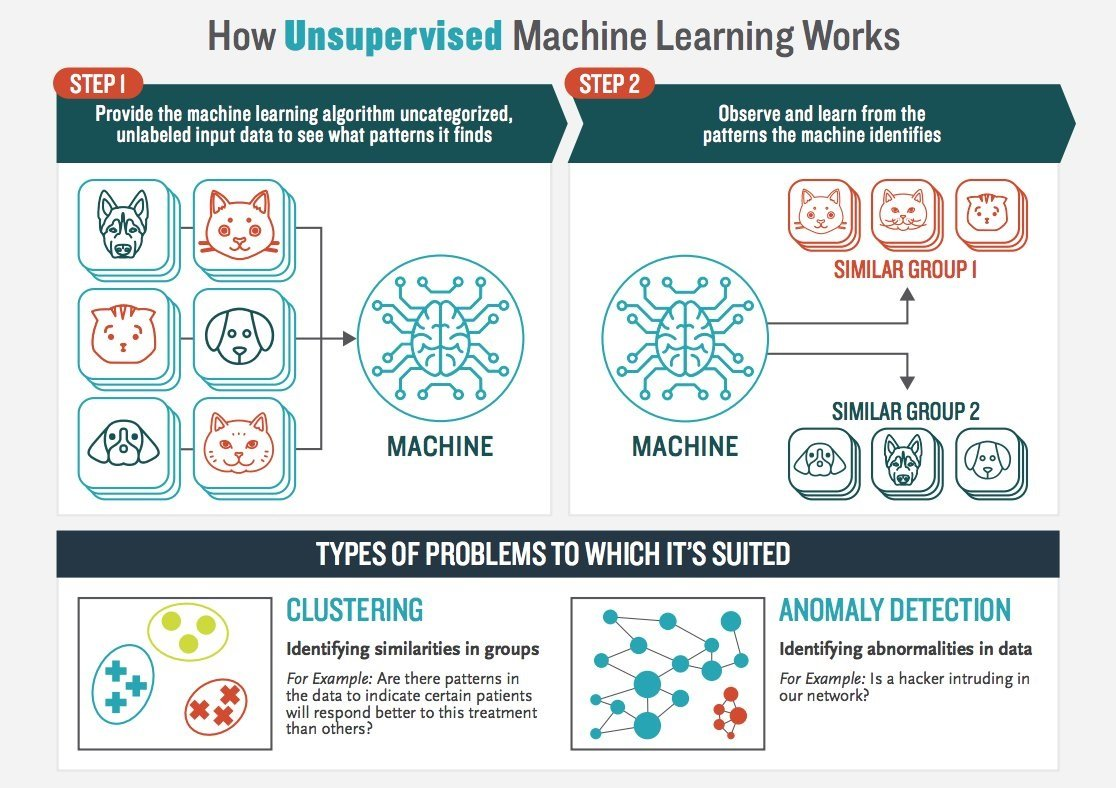
\includegraphics[width=1\textwidth]{figures/1174006/chapter1/unsupervisedlearning.jpg}
	\centering
	\caption{Unsupervised Learning.}
\end{figure}
\noindent
Tetapi unsupervise learning tidak memiliki outcome yang spesifik layaknya di supervise learning, hal ini dikarenakan tidak adanya ground truth / label dasar. Walaupun begitu, unsupervised learning masih dapat memprediksi dari ketidakadaan label dari kemiripan attribute yang dimilik data.
\noindent
Algoritma yang digunakan di unsupervised learning :
\begin{enumerate}
	\item Clustering
    \item Anomaly Detection
    \item Training Model
    \item Association Discovery
\end{enumerate}
\subsubsection{Data Set}
\hfill\break
Dataset adalah objek yang merepresentasikan data dan relasinya di memory. Strukturnya mirip dengan data di database. Dataset berisi koleksi dari datatable dan data relation.
\subsubsection{Training Set}
\hfill\break
Training set adalah bagian dataset yang kita latih untuk membuat prediksi atau menjalankan fungsi dari sebuah algoritma ML lainnya sesuai tujuannya masing-masing. Kita memberikan petunjuk melalui algoritma agar mesin yang kita latih bisa mencari korelasinya sendiri. 
\subsubsection{Testing Set}
\hfill\break
Test set adalah bagian dataset yang kita tes untuk melihat keakuratannya, atau dengan kata lain melihat performanya.
\subsection{Praktek}
\begin{enumerate}
	\item Instalasi  library  scikit  dari  anaconda,  mencoba  kompilasi  dan  uji  coba  ambil contoh kode dan lihat variabel explorer.
	
	\textbf{Instalasi Library Scikit-Learn dengan Anaconda}
	\begin{enumerate}
		\item Pertama pastikan anda telah menginstall Anaconda. Jika sudah menginstall Anaconda, jalankan Anaconda Navigator.
		\begin{figure}[H]
			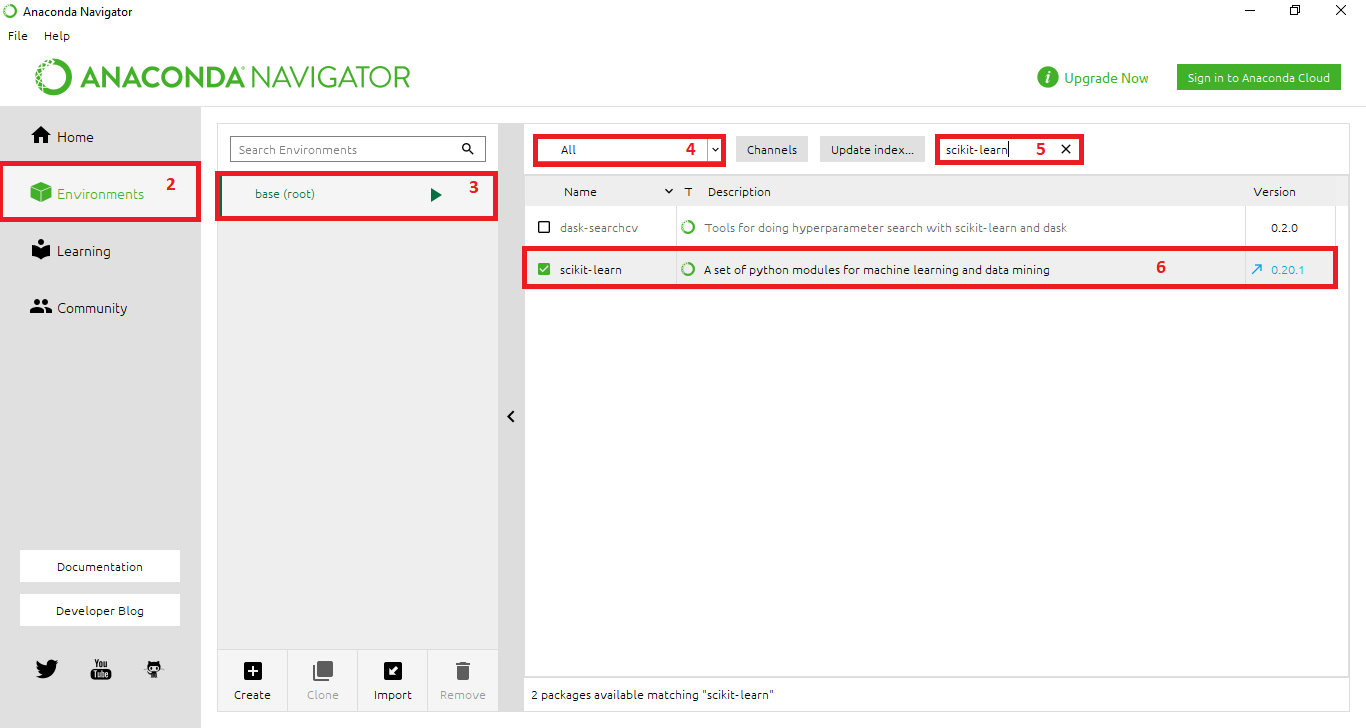
\includegraphics[width=1\textwidth]{figures/1174006/chapter1/praktek/install.png}
			\centering
			\caption{Instalasi Library Scikit-Learn.}
		\end{figure}
		\item Selanjutnya klik menu Environment.
		\item Kemudian klik environment base(root). Disini kita akan melakukan instalasi library scikit- learn di environment base(root).
		\item Lalu pilih All. Untuk menampilkan list library yang ada.
		\item Setelah itu cari scikit-learn di kolom pencarian.
		\item Selanjutnya centang library scikit-learn, lalu klik tombol Apply.
	\end{enumerate}

	\textbf{Mencoba Menggunakan Library scikit-Learn}
	\begin{enumerate}
		\item Pertama jalankan aplikasi Spyder.
		\item Kemudian buat file baru, lalu tambahkan kode berikut.
		\lstinputlisting[language=Python]{src/1174006/chapter1/contoh.py}
		\item Simpan dan jalankan.
		\item Hasil dari variabel explorernya sebagai berikut.
		\begin{figure}[H]
			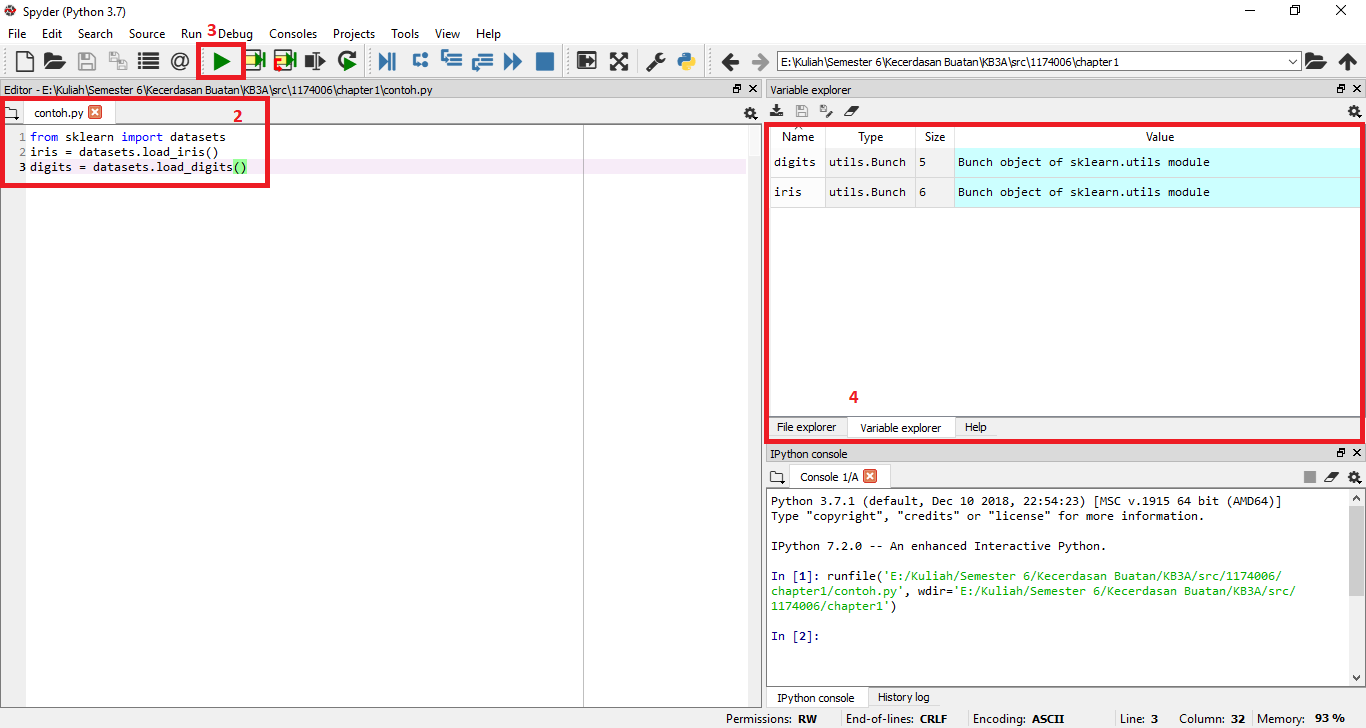
\includegraphics[width=1\textwidth]{figures/1174006/chapter1/praktek/variabel.png}
			\centering
			\caption{Variabel Explorer Library Scikit-Learn.}
		\end{figure}
	\end{enumerate}
	
	\item Mencoba Loading an example dataset, menjelaskan maksud dari tulisan terse-but dan mengartikan per baris.
	\lstinputlisting[language=Python]{src/1174006/chapter1/coba1.py}
	
	Hasilnya akan seperti ini.
	\begin{figure}[H]
		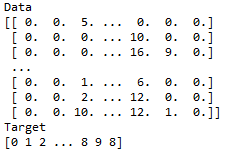
\includegraphics[width=5cm]{figures/1174006/chapter1/praktek/coba1.png}
		\centering
		\caption{Hasil Loading an Example Dataset.}
	\end{figure}

	\item Mencoba  Learning  and  predicting,  menjelaskan  maksud  dari  tulisan  tersebut dan mengartikan per baris.
	\lstinputlisting[language=Python]{src/1174006/chapter1/coba2.py}
	
	Hasilnya akan seperti ini.
	\begin{figure}[H]
		
\includegraphics[width=1cm]{figures/1174006/chapter1/praktek/coba2.png}
		\centering
		\caption{Hasil Learning and Predicting.}
	\end{figure}

	\item Mencoba Model persistence, menjelaskan maksud dari tulisan tersebut dan mengartikan per baris.
	\lstinputlisting[language=Python]{src/1174006/chapter1/coba3.py}
	
	Hasilnya akan seperti ini.
	\begin{figure}[H]
		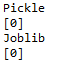
\includegraphics[width=2cm]{figures/1174006/chapter1/praktek/coba3.png}
		\centering
		\caption{Hasil Model Persistence.}
	\end{figure}

	\item Mencoba Conventions, menjelaskan maksud dari tulisan tersebut dan mengartikan per baris.
	\lstinputlisting[language=Python]{src/1174006/chapter1/coba4.py}
	
	Hasilnya akan seperti ini.
	\begin{figure}[H]
		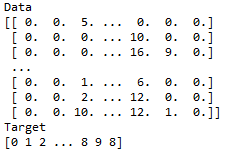
\includegraphics[width=5cm]{figures/1174006/chapter1/praktek/coba1.png}
		\centering
		\caption{Hasil Conventions.}
	\end{figure}

\end{enumerate}

\subsection{Penanganan Error}
\begin{enumerate}
	\item Skrinsut error.
	\begin{itemize}
		\item Name Error
		\hfill\break
		\begin{figure}[H]
			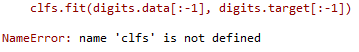
\includegraphics[width=1\textwidth]{figures/1174006/chapter1/error/err3.png}
			\centering
			\caption{Name Error.}
		\end{figure}
		\item Import Error
		\hfill\break
		\begin{figure}[H]
			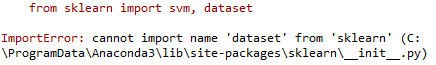
\includegraphics[width=1\textwidth]{figures/1174006/chapter1/error/err1.png}
			\centering
			\caption{Import Error.}
		\end{figure}
		\item Value Error
		\hfill\break
		\begin{figure}[H]
			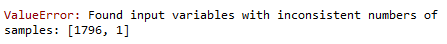
\includegraphics[width=1\textwidth]{figures/1174006/chapter1/error/err2.png}
			\centering
			\caption{Value Error.}
		\end{figure}
		\item Syntax Error
		\hfill\break
		\begin{figure}[H]
			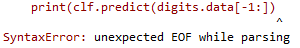
\includegraphics[width=1\textwidth]{figures/1174006/chapter1/error/err4.png}
			\centering
			\caption{Syntax Error.}
		\end{figure}
	\end{itemize}
	\item Tuliskan kode eror dan jenis errornya.
	\begin{itemize}
		\item Name Error
		\hfill\break
		Name Error adalah exception yang terjadi saat syntax melakukan eksekusi terhadap local name atau global name yang tidak terdefinisi.
		\item Import Error
		\hfill\break
		Import Error adalah exception yang terjadi saat syntax melakukan import terhadap library yang tidak terdefinisi.
		\item Value Error
		\hfill\break
		Value Error adalah exception yang terjadi saat syntax memiliki nilai yang tidak valid.
		\item Syntax Error
		\hfill\break
		Syntax Error adalah exception yang terjadi saat ada kesalahan dalam mengetikkan syntax.
	\end{itemize}
	\item Solusi pemecahan masalah error tersebut.
	\begin{itemize}
		\item Name Error
		\hfill\break
		Solusinya adalah memastikan variabel atau function yang dipanggil ada atau tidak salah ketik.
		\item Import Error
		\hfill\break
		Solusinya adalah memastikan library yang dipanggil ada atau tidak salah ketik.
		\item Value Error
		\hfill\break
		Solusinya adalah memastikan nilai yang diinputkan valid.
		\item Syntax Error
		\hfill\break
		Solusinya adalah memastikan syntax yang diketik tidak salah ketik.
	\end{itemize}
\end{enumerate}

\subsection{Bukti Tidak Plagiat}
\begin{figure}[H]
	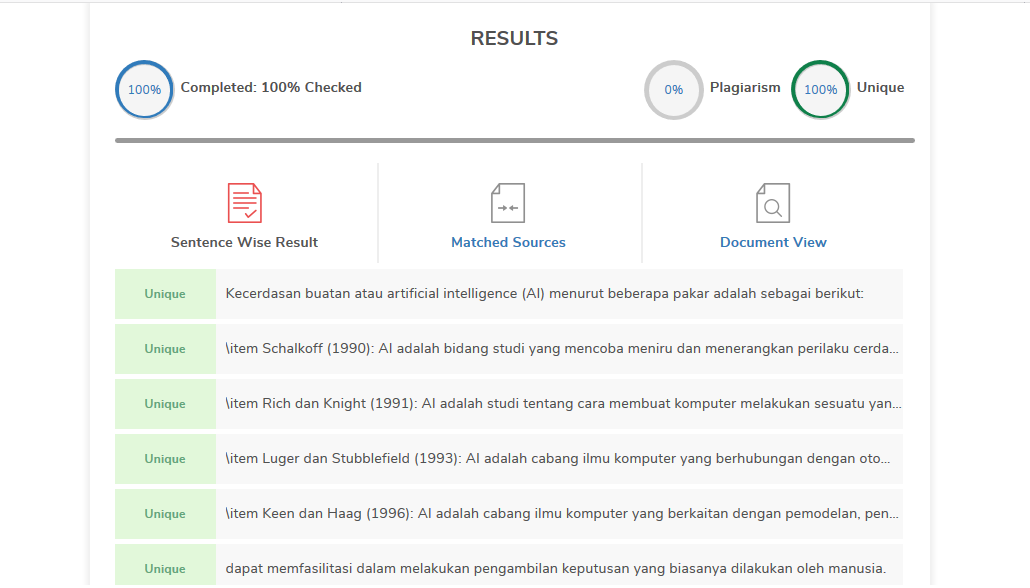
\includegraphics[width=1\textwidth]{figures/1174006/chapter1/plagiat.png}
	\centering
	\caption{Bukti Tidak Plagiat.}
\end{figure}
%\section{1174027 - Harun Ar - Rasyid}
\subsection{Teori}
\begin{enumerate}
	\item Sejarah dan Perkembangan
	\hfill\break
	Kecerdasan Buatan atau dalam Bahasa inggris sering disebut Artifical Intelligence yang sering disebut juga sebagai AI, pada 10 tahun lalu masyarakat belum terlalu mengetahui hal tersebut dan masih menjadi bahan candaan dikalangan masyarakat. Awal perkembangan AI dimulai pada tahun 1952-1969 yang dimulai dengan kesuksesan Newwll dan temannya simon menggunakan sebuah program yang disebut dengan General Problem Solver. Program ini dibangun untuk tujuan penyelesaiin masalah secara manusiawi. Pada tahun 1966-1974 perkembangan kecerdasan buatan mulai melambat. Ada 3 faktor utama yang menyebabkan hal itu terjadi:
	\begin{itemize}
		\item Banyak subjek pada program AI yang bermunculan hanya mengandung sedikit atau bahkan sama sekali tidak  mengandung sama sekali pengetahuan (knowledge).
		\item Kecerdasan buatan harus bisa menyelesaikan banyak masalah.
		\item Untuk menghasilkan perilkau intelijensia ada beberapa batasan pada struktur yang bisa digunakan.
	\end{itemize}
	Definisi kecerdasan buatan itu sendiri adalah suatu system teknologi yang didalamnya ditambahakan kecerdasan oleh manusia, kecerdasan buatan diatur dan dikembangkan dalam konteks ilmiah, dan bentukan dari kecerdasan entitas ilmiah yang ada.
	\item Definisi
	\hfill\break
	Supervised learning, klasifikasi, regresi, unsupervised learning, dataset, trainingset dan testingset.
	\begin{itemize}
		\item Supervised Learning
		\hfill\break
		Supervised Learning merupakan sebuah tipe learning yang mempunyai variable input dan variable output, tipe ini juga menggunakan satu algoritma atau lebih dari satu algoritma yang digunakan untuk mempelajari fungsi  pemetaan dari input ke output.
		\item Klasifikasi
		\hfill\break
		Klasifikasi adalah pengelompokan data di mana data yang digunakan memiliki label atau kelas target. Sehingga algoritma untuk menyelesaikan masalah klasifikasi dikategorikan ke dalam pembelajaran terbimbing.
		\item Regresi
		\hfill\break
		regressi metode analisis statistik yang digunakan untuk dapat melihat efek antara dua atau lebih variabel. Hubungan variabel dalam pertanyaan adalah fungsional yang diwujudkan dalam bentuk model matematika. Dalam analisis regresi, variabel dibagi menjadi dua jenis, yaitu variabel respons atau yang biasa disebut variabel dependen dan variabel independen atau dikenal sebagai variabel independen. Ada beberapa jenis analisis regresi, yaitu regresi sederhana yang mencakup linear sederhana dan regresi non-linear sederhana dan regresi berganda yang mencakup banyak linier atau non-linear berganda. Analisis regresi digunakan dalam pembelajaran mesin pembelajaran dengan metode pembelajaran terawasi.
		\item Unsupervised learning 
		\hfill\break
		unsupervised learning jenis pembelajaran di mana kita hanya memiliki data input (input data) tetapi tidak ada variabel output yang terkait. Tujuan dari pembelajaran tanpa pengawasan adalah untuk memodelkan struktur dasar atau distribusi data dengan tujuan mempelajari data lebih lanjut, dengan kata lain, itu adalah fungsi simpulan yang menggambarkan atau menjelaskan data.
		\item Data set
		\hfill\break
		Data set objek yang merepresentasikan data dan relasinya di memory. Strukturnya mirip dengan data di database. Dataset berisi koleksi dari datatable dan datarelation.
		\item Training Set
		\hfill\break
		Training set adalah bagian dari dataset yang di latih untuk membuat prediksi atau menjalankan fungsi dari algoritma ML lain sesuai dengan masing-masing. Memberikan instruksi melalui algoritma sehingga mesin yang di praktikkan dapat menemukan korelasinya sendiri.
		\item Testing Set
		\hfill\break
		testing set adalah bagian dari dataset yang kami uji untuk melihat akurasinya, atau dengan kata lain untuk melihat kinerjanya.
	\end{itemize}
\end{enumerate}
\subsection{Praktek}
\begin{enumerate}
	\item Instalasi Library scikit dari ianaconda, mencoba kompilasi dan uji coba ambil contoh kode dan lihat variabel explorer
	\hfill\break
	\begin{figure}[H]
		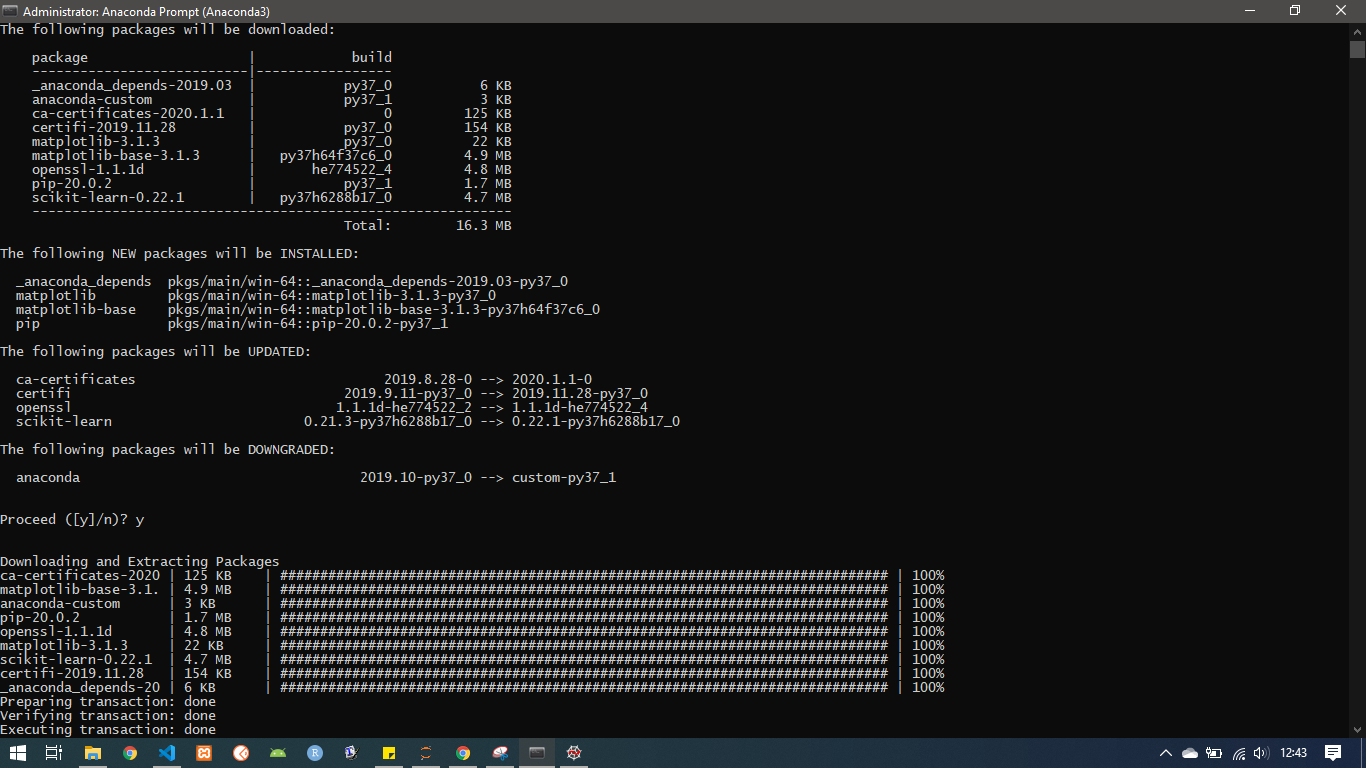
\includegraphics[width=4cm]{figures/1174027/1/instalasi.png}
		\centering
		\caption{Instalasi Package Scikit Learn}
	\end{figure}
	\begin{figure}[H]
		\includegraphics[width=4cm]{figures/1174027/1/variabel.png}
		\centering
		\caption{Isi Variabel Explorer}
	\end{figure}
	\item Mencoba loading an example dataset
	\hfill\break
	\lstinputlisting[firstline=7, lastline=11]{src/1174027/1/1174027.py}
	\item Mencoba Learning dan predicting
	\hfill\break
	\lstinputlisting[firstline=13, lastline=22]{src/1174027/1/1174027.py}
	\item Mencoba Model Persistence
	\hfill\break
	\lstinputlisting[firstline=25, lastline=34]{src/1174027/1/1174027.py}
	\item Mencoba Conventions
	\hfill\break
	\lstinputlisting[firstline=37, lastline=48]{src/1174027/1/1174027.py}
\end{enumerate}
\subsection{Penanganan Error}
\begin{enumerate}
	\item ScreenShoot Error
	\begin{figure}[H]
		\includegraphics[width=4cm]{figures/1174027/error/1_import.png}
		\centering
		\caption{Import Error}
	\end{figure}
	\begin{figure}[H]
		\includegraphics[width=4cm]{figures/1174027/error/1_value.png}
		\centering
		\caption{Value Error}
	\end{figure}
	\item Tuliskan Kode Error dan Jenis Error
	\begin{itemize}
		\item Import Error
		\item Value Error
	\end{itemize}
	\item Cara Penangan Error
	\begin{itemize}
		\item Import Error
		\hfill\break
		Dengan Menginstall Library Yang Tidak Ditemukan
		\item Value Error
		\hfill\break
		Mengubah Bentuk Arraynya, Menjadi 1 Dimensi
	\end{itemize}
\end{enumerate}
\subsection{Bukti Tidak Plagiat}
\begin{figure}[H]
	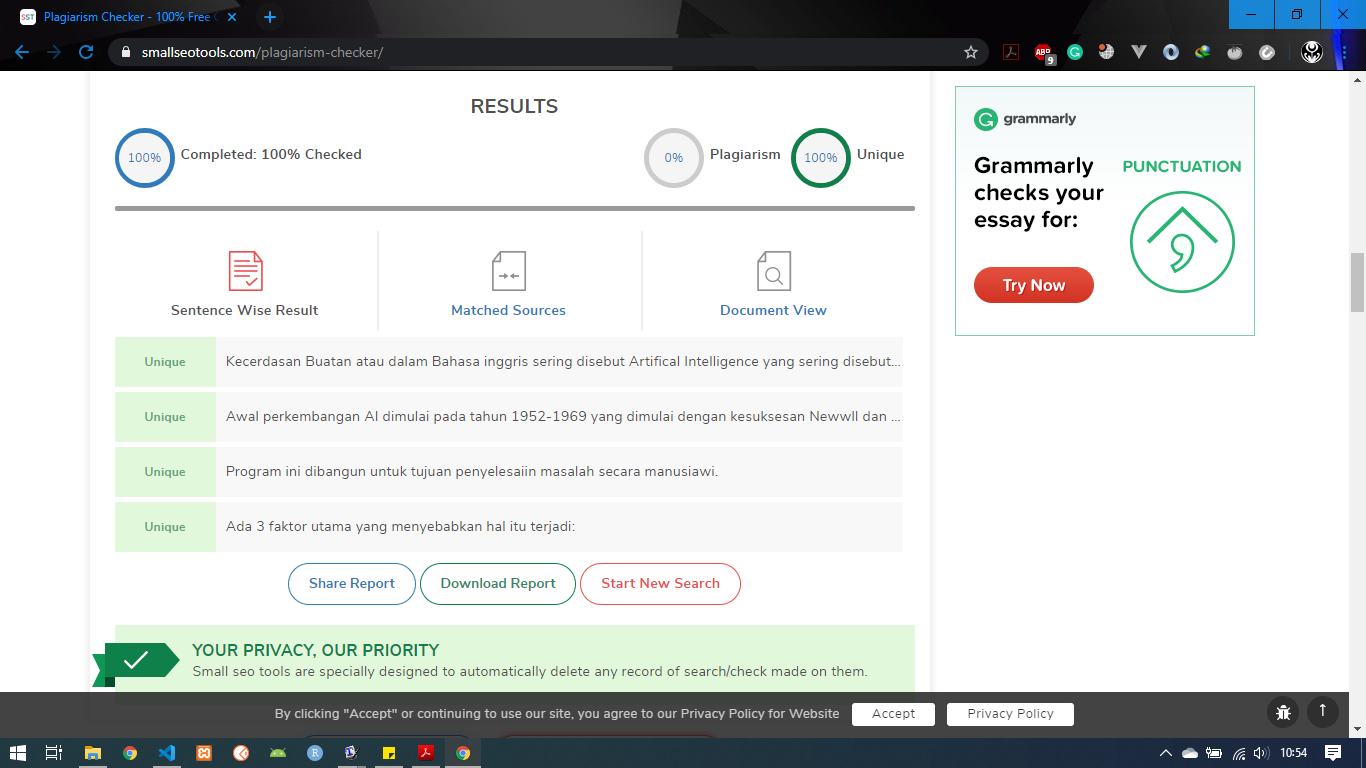
\includegraphics[width=4cm]{figures/1174027/bukti/1.png}
	\centering
	\caption{Bukti Tidak Melakukan Plagiat Chapter 1}
\end{figure}
%\section{1174031 - Muhammad Tomy Nur Maulidy}
\subsection{Teori}
\begin{enumerate}
	\item Sejarah dan Perkembangan
	\hfill\break
	Kecerdasan Buatan atau dalam Bahasa inggris sering disebut Artifical Intelligence yang sering disebut juga sebagai AI, pada 10 tahun lalu masyarakat belum terlalu mengetahui hal tersebut dan masih menjadi bahan candaan dikalangan masyarakat. Awal perkembangan AI dimulai pada tahun 1952-1969 yang dimulai dengan kesuksesan Newwll dan temannya simon menggunakan sebuah program yang disebut dengan General Problem Solver. Program ini dibangun untuk tujuan penyelesaiin masalah secara manusiawi. Pada tahun 1966-1974 perkembangan kecerdasan buatan mulai melambat. Ada 3 faktor utama yang menyebabkan hal itu terjadi:
	\begin{itemize}
		\item Banyak subjek pada program AI yang bermunculan hanya mengandung sedikit atau bahkan sama sekali tidak  mengandung sama sekali pengetahuan (knowledge).
		\item Kecerdasan buatan harus bisa menyelesaikan banyak masalah.
		\item Untuk menghasilkan perilkau intelijensia ada beberapa batasan pada struktur yang bisa digunakan.
	\end{itemize}
	Definisi kecerdasan buatan itu sendiri adalah suatu system teknologi yang didalamnya ditambahakan kecerdasan oleh manusia, kecerdasan buatan diatur dan dikembangkan dalam konteks ilmiah, dan bentukan dari kecerdasan entitas ilmiah yang ada.
	\item Definisi
	\hfill\break
	Supervised learning, klasifikasi, regresi, unsupervised learning, dataset, trainingset dan testingset.
	\begin{itemize}
		\item Supervised Learning
		\hfill\break
		Supervised Learning merupakan sebuah tipe learning yang mempunyai variable input dan variable output, tipe ini juga menggunakan satu algoritma atau lebih dari satu algoritma yang digunakan untuk mempelajari fungsi  pemetaan dari input ke output.
		\item Klasifikasi
		\hfill\break
		Klasifikasi adalah pengelompokan data di mana data yang digunakan memiliki label atau kelas target. Sehingga algoritma untuk menyelesaikan masalah klasifikasi dikategorikan ke dalam pembelajaran terbimbing.
		\item Regresi
		\hfill\break
		regressi metode analisis statistik yang digunakan untuk dapat melihat efek antara dua atau lebih variabel. Hubungan variabel dalam pertanyaan adalah fungsional yang diwujudkan dalam bentuk model matematika. Dalam analisis regresi, variabel dibagi menjadi dua jenis, yaitu variabel respons atau yang biasa disebut variabel dependen dan variabel independen atau dikenal sebagai variabel independen. Ada beberapa jenis analisis regresi, yaitu regresi sederhana yang mencakup linear sederhana dan regresi non-linear sederhana dan regresi berganda yang mencakup banyak linier atau non-linear berganda. Analisis regresi digunakan dalam pembelajaran mesin pembelajaran dengan metode pembelajaran terawasi.
		\item Unsupervised learning 
		\hfill\break
		unsupervised learning jenis pembelajaran di mana kita hanya memiliki data input (input data) tetapi tidak ada variabel output yang terkait. Tujuan dari pembelajaran tanpa pengawasan adalah untuk memodelkan struktur dasar atau distribusi data dengan tujuan mempelajari data lebih lanjut, dengan kata lain, itu adalah fungsi simpulan yang menggambarkan atau menjelaskan data.
		\item Data set
		\hfill\break
		Data set objek yang merepresentasikan data dan relasinya di memory. Strukturnya mirip dengan data di database. Dataset berisi koleksi dari datatable dan datarelation.
		\item Training Set
		\hfill\break
		Training set adalah bagian dari dataset yang di latih untuk membuat prediksi atau menjalankan fungsi dari algoritma ML lain sesuai dengan masing-masing. Memberikan instruksi melalui algoritma sehingga mesin yang di praktikkan dapat menemukan korelasinya sendiri.
		\item Testing Set
		\hfill\break
		testing set adalah bagian dari dataset yang kami uji untuk melihat akurasinya, atau dengan kata lain untuk melihat kinerjanya.
	\end{itemize}
\end{enumerate}
\subsection{Praktek}
\begin{enumerate}
	\item Instalasi Library scikit dari ianaconda, mencoba kompilasi dan uji coba ambil contoh kode dan lihat variabel explorer
	\hfill\break
	\begin{figure}[H]
		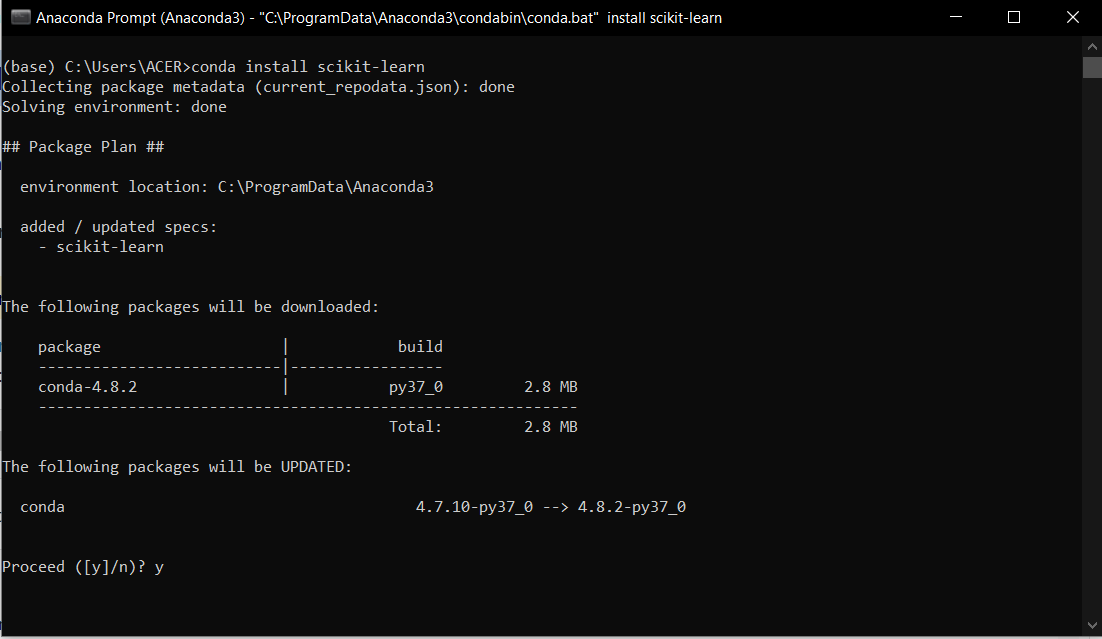
\includegraphics[width=4cm]{figures/1174031/1/1.PNG}
		\centering
		\caption{Instalasi Package Scikit Learn}
	\end{figure}
	\begin{figure}[H]
		\includegraphics[width=4cm]{figures/1174031/1/2.PNG}
		\centering
		\caption{Isi Variabel Explorer}
	\end{figure}
	\item Mencoba loading an example dataset
	\hfill\break
	\lstinputlisting[firstline=8, lastline=12]{src/1174031/1/1174031.py}
	\item Mencoba Learning dan predicting
	\hfill\break
	\lstinputlisting[firstline=14, lastline=24]{src/1174031/1/1174031.py}
	\item Mencoba Model Persistence
	\hfill\break
	\lstinputlisting[firstline=26, lastline=36]{src/1174031/1/1174031.py}
	\item Mencoba Conventions
	\hfill\break
	\lstinputlisting[firstline=38, lastline=50]{src/1174031/1/1174031.py}
\end{enumerate}
\subsection{Penanganan Error}
\begin{enumerate}
	\item ScreenShoot Error
	\begin{figure}[H]
		\includegraphics[width=4cm]{figures/1174031/1/error/1.png}
		\centering
		\caption{Import Error}
	\end{figure}
	\begin{figure}[H]
		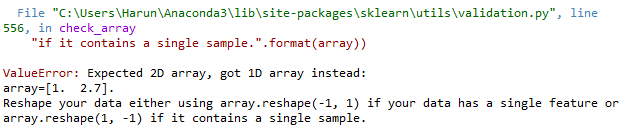
\includegraphics[width=4cm]{figures/1174031/1/error/2.png}
		\centering
		\caption{Value Error}
	\end{figure}
	\item Tuliskan Kode Error dan Jenis Error
	\begin{itemize}
		\item Import Error
		\item Value Error
	\end{itemize}
	\item Cara Penangan Error
	\begin{itemize}
		\item Import Error
		\hfill\break
		Dengan Menginstall Library Yang Tidak Ditemukan
		\item Value Error
		\hfill\break
		Mengubah Bentuk Arraynya, Menjadi 1 Dimensi
	\end{itemize}
\end{enumerate}
\subsection{Bukti Tidak Plagiat}
\begin{figure}[H]
	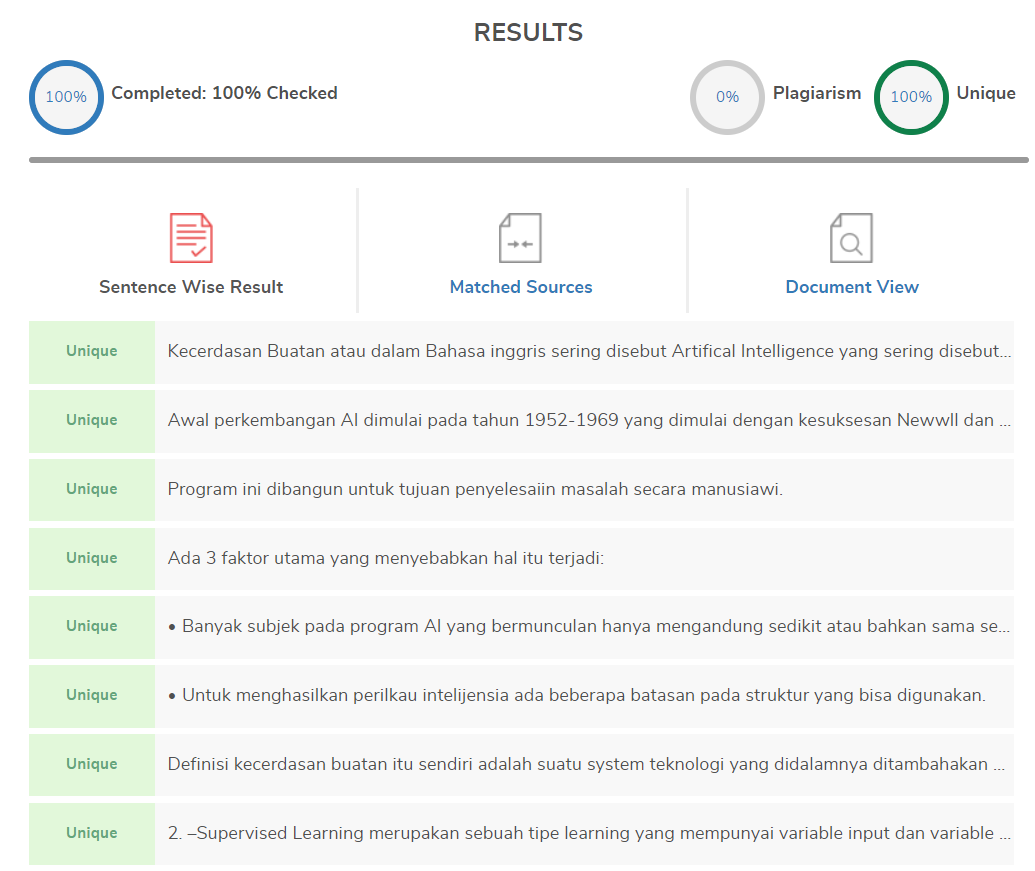
\includegraphics[width=4cm]{figures/1174031/1/plagiat/1.PNG}
	\centering
	\caption{Bukti Tidak Melakukan Plagiat 1}
    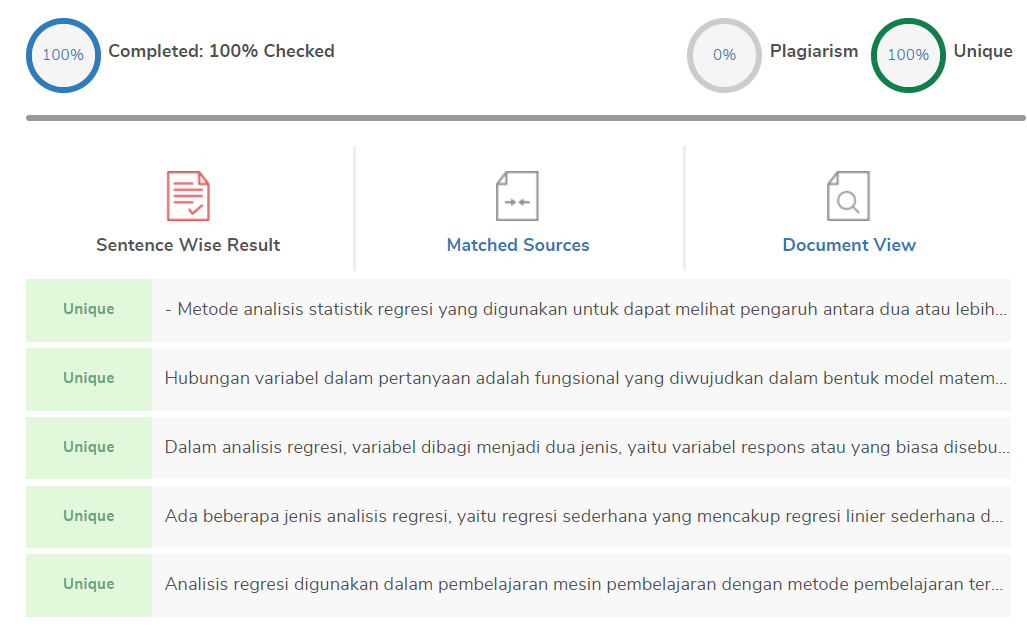
\includegraphics[width=4cm]{figures/1174031/1/plagiat/2.PNG}
	\centering
	\caption{Bukti Tidak Melakukan Plagiat 2}
\end{figure}
%\section{1174003 - Dwi Septiani Tsaniyah}
\subsection{Teori}
\begin{enumerate}
	\item Sejarah dan Perkembangan
	\hfill\break
	Kecerdasan buatan adalah bidang ilmu komputer yang sangat penting di masa kini dan masa depan untuk mewujudkan sistem komputer cerdas. "Intelligo" yang berarti "Saya mengerti". Berarti dasar kecerdasan untuk mengatasi dan mengambil tindakan. Sebenarnya, bidang Artificial Intelligence, atau disingkat AI, yang diambil dari tampilan komputer sekitar tahun 1940-an, sedangkan sejarah perkembangannya dapat ditelusuri sejak zaman Mesir kuno. Pada saat ini, perhatian diberikan pada kemampuan komputer untuk melakukan hal-hal yang dapat dilakukan manusia. Dalam hal ini, komputer dapat menggunakan kecerdasan dan komunikasi manusia McMulloh dan Pitts pada tahun 1943 meminta model matematika yang disebut perceptron neuron di otak. Mereka juga menunjukkan bagaimana neuron menjadi aktif seperti sakelar on-off dan neuron dapat belajar dan memberikan tindakan yang berbeda dari input yang diberikan. Kontribusi terbesar dalam bidang AI dimulai dengan karya Alan Turing, pada tahun 1950 yang mencoba menjawab "Can computer think" dengan menciptakan mesin Turing. Makalah Alan Turing tahun 1950 berjudul "Mesin Komputer dan Kecerdasan" membahas istilah-istilah mesin yang dianggap cerdas. Dia berasumsi bahwa jika sebuah mesin dapat berhasil berperilaku seperti manusia, kita dapat menganggapnya sebagai kecerdasan. Ada 3 faktor utama yang menyebabkan hal itu terjadi:
	\begin{itemize}
		\item Banyak subjek pada program AI yang bermunculan hanya mengandung sedikit atau bahkan sama sekali tidak  mengandung sama sekali pengetahuan (knowledge).
		\item Kecerdasan buatan harus bisa menyelesaikan banyak masalah.
		\item Untuk menghasilkan perilkau intelijensia ada beberapa batasan pada struktur yang bisa digunakan.
	\end{itemize}
	Definisi kecerdasan buatan itu sendiri adalah suatu system teknologi yang didalamnya ditambahakan kecerdasan oleh manusia, kecerdasan buatan diatur dan dikembangkan dalam konteks ilmiah, dan bentukan dari kecerdasan entitas ilmiah yang ada.
	\item Definisi
	\hfill\break
	Supervised learning, klasifikasi, regresi, unsupervised learning, dataset, trainingset dan testingset.
	\begin{itemize}
		\item Supervised Learning
		\hfill\break
		Supervised Learning merupakan sebuah tipe learning yang mempunyai variable input dan variable output, tipe ini juga menggunakan satu algoritma atau lebih dari satu algoritma yang digunakan untuk mempelajari fungsi  pemetaan dari input ke output.
		\item Klasifikasi
		\hfill\break
		Klasifikasi adalah pengelompokan data di mana data yang digunakan memiliki label atau kelas target. Sehingga algoritma untuk menyelesaikan masalah klasifikasi dikategorikan ke dalam pembelajaran terbimbing.
		\item Regresi
		\hfill\break
		regressi metode analisis statistik yang digunakan untuk dapat melihat efek antara dua atau lebih variabel. Hubungan variabel dalam pertanyaan adalah fungsional yang diwujudkan dalam bentuk model matematika. Dalam analisis regresi, variabel dibagi menjadi dua jenis, yaitu variabel respons atau yang biasa disebut variabel dependen dan variabel independen atau dikenal sebagai variabel independen. Ada beberapa jenis analisis regresi, yaitu regresi sederhana yang mencakup linear sederhana dan regresi non-linear sederhana dan regresi berganda yang mencakup banyak linier atau non-linear berganda. Analisis regresi digunakan dalam pembelajaran mesin pembelajaran dengan metode pembelajaran terawasi.
		\item Unsupervised learning 
		\hfill\break
		unsupervised learning jenis pembelajaran di mana kita hanya memiliki data input (input data) tetapi tidak ada variabel output yang terkait. Tujuan dari pembelajaran tanpa pengawasan adalah untuk memodelkan struktur dasar atau distribusi data dengan tujuan mempelajari data lebih lanjut, dengan kata lain, itu adalah fungsi simpulan yang menggambarkan atau menjelaskan data.
		\item Data set
		\hfill\break
		Data set objek yang merepresentasikan data dan relasinya di memory. Strukturnya mirip dengan data di database. Dataset berisi koleksi dari datatable dan datarelation.
		\item Training Set
		\hfill\break
		Training set adalah bagian dari dataset yang di latih untuk membuat prediksi atau menjalankan fungsi dari algoritma ML lain sesuai dengan masing-masing. Memberikan instruksi melalui algoritma sehingga mesin yang di praktikkan dapat menemukan korelasinya sendiri.
		\item Testing Set
		\hfill\break
		testing set adalah bagian dari dataset yang kami uji untuk melihat akurasinya, atau dengan kata lain untuk melihat kinerjanya.
	\end{itemize}
\end{enumerate}
\subsection{Praktek}
\begin{enumerate}
	\item Instalasi Library scikit dari ianaconda, mencoba kompilasi dan uji coba ambil contoh kode dan lihat variabel explorer
	\hfill\break
	\begin{figure}[H]
		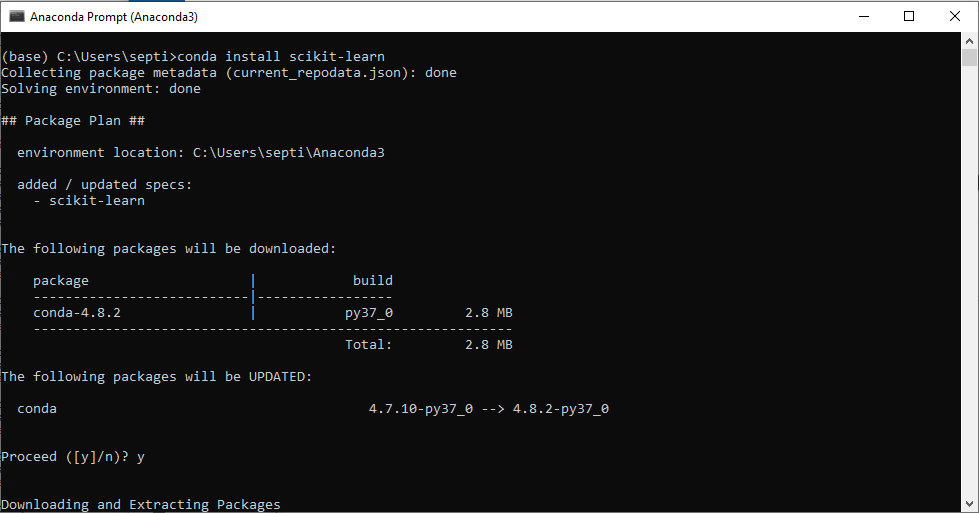
\includegraphics[width=4cm]{figures/1174003/1/1.PNG}
		\centering
		\caption{Instalasi Package Scikit Learn}
	\end{figure}
	\begin{figure}[H]
		\includegraphics[width=4cm]{figures/1174003/1/2.PNG}
		\centering
		\caption{Isi Variabel Explorer}
	\end{figure}
	\item Mencoba loading an example dataset
	\hfill\break
	\lstinputlisting[firstline=8, lastline=12]{src/1174003/1/1174003.py}
	\item Mencoba Learning dan predicting
	\hfill\break
	\lstinputlisting[firstline=14, lastline=24]{src/1174003/1/1174003.py}
	\item Mencoba Model Persistence
	\hfill\break
	\lstinputlisting[firstline=26, lastline=36]{src/1174003/1/1174003.py}
	\item Mencoba Conventions
	\hfill\break
	\lstinputlisting[firstline=38, lastline=50]{src/1174003/1/1174003.py}
\end{enumerate}
\subsection{Penanganan Error}
\begin{enumerate}
	\item ScreenShoot Error
	\begin{figure}[H]
		\includegraphics[width=4cm]{figures/1174031/1/error/1.png}
		\centering
		\caption{Import Error}
	\end{figure}
	\begin{figure}[H]
		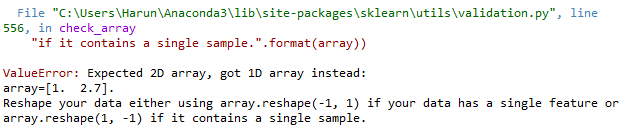
\includegraphics[width=4cm]{figures/1174031/1/error/2.png}
		\centering
		\caption{Value Error}
	\end{figure}
	\item Tuliskan Kode Error dan Jenis Error
	\begin{itemize}
		\item Import Error
		\item Value Error
	\end{itemize}
	\item Cara Penangan Error
	\begin{itemize}
		\item Import Error
		\hfill\break
		Dengan Menginstall Library Yang Tidak Ditemukan
		\item Value Error
		\hfill\break
		Mengubah Bentuk Arraynya, Menjadi 1 Dimensi
	\end{itemize}
\end{enumerate}
\subsection{Bukti Tidak Plagiat}
\begin{figure}[H]
	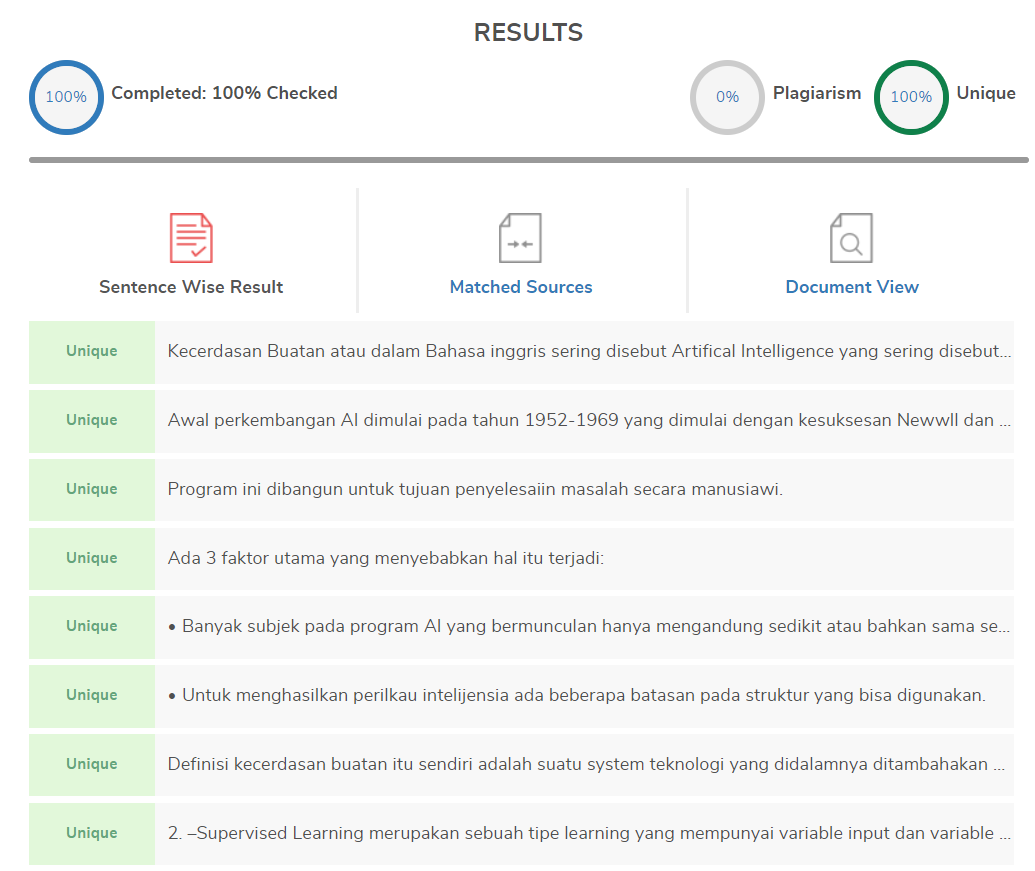
\includegraphics[width=4cm]{figures/1174031/1/plagiat/1.PNG}
	\centering
	\caption{Bukti Tidak Melakukan Plagiat 1}
\end{figure}
%\section{1174051 - Evietania Charis Sujadi}
\subsection{Teori}
\begin{enumerate}
\item Definisi, sejarah, dan juga pengembangan Kecerdasan Buatan
\subitem Definisi kecerdasan diciptakan oleh pengetahuan yang dapat membuat komputer untuk kecerdasan manusia terkait dengan penangkapan, pemodelan, dan penyimpanan kecerdasan manusia dalam suatu sistem teknologi. Contohnya adalah melakukan analisis penalti untuk menarik kesimpulan atau menerjemahkan kelemahan atau memutuskan dari satu bahasa ke bahasa lain.
\subitem Sejarah dan perkembangan intelijen terjadi pada musim panas 1956 menerima seminar tentang AI di Darmouth College. Seminar dihadiri oleh para ahli komputer dan membahas potensi komputer dalam pengaduan kecerdasan manusia. Namun, perkembangan yang sudah sering terjadi sejak LISP diciptakan, yaitu kecerdasan buatan yang dibuat pada tahun 1960 oleh John McCarthy. Istilah kecerdasan buatan atau Inteligensi Buatan diambil dari Marvin Minsky dari MIT. Dia menulis sebuah makalah ilmiah yang berjudul Steps to Artificial Intelligence, Institute for Proceedings of Radio Engineers 49, Januari 1961. 
\item  Definisi supervised learning, klasifikasi, regresi, dan unsupervised learning. Data set, training set dan testing set. 
\subitem Supervised learning merupakan sebuah pendekatan dimana sudah terdapat data yang dilatih, dan terdapat variable yang ditargetkan sehingga tujuan dari pendekatan ini adalah mengkelompokan suatu data ke data yang sudah ada. Sedangkan unsupervised learning tidak memiliki data latih, sehingga dari data yang ada, kita mengelompokan data tersebut menjadi 2 bagian atau 3 bagian dan seterusnya.
\subitem Klasifikasi adalah salah satu topik utama dalam data mining atau machine learning. Klasifikasi yaitu suatu pengelompokan data dimana data yang digunakan tersebut mempunyai kelas label atau target.
\subitem Regresi adalah Supervised learning tidak hanya mempelajari classifier, tetapi juga mempelajari fungsi yang dapat memprediksi suatu nilai numerik. Contoh, ketika diberi foto seseorang, kita ingin memprediksi umur, tinggi, dan berat orang yang ada pada foto tersebut.
\subitem Data set adalah cabang aplikasi dari Artificial Intelligence/Kecerdasan Buatan yang fokus pada pengembangan sebuah sistem yang mampu belajar sendiri tanpa harus berulang kali di program oleh manusia.
\subitem Training set yaitu jika pasangan objek, dan kelas yang menunjuk pada objek tersebut adalah suatu contoh yang telah diberi label akan menghasilkan suatu algoritma pembelajaran.
\subitem Tujuan dari set tes adalah untuk menentukan sejauh mana classifier berhasil membuat klasifikasi dengan benar
\end{enumerate}
\subsection{Instalasi}
\begin{enumerate}
\item {Instalasi Library Scikit}
Masuk pada windows lalu search "conda" , setelah itu akan muncul Anaconda prompt. lalu ketikkan conda install scikit-learn
\begin{figure}[ht]
\centering
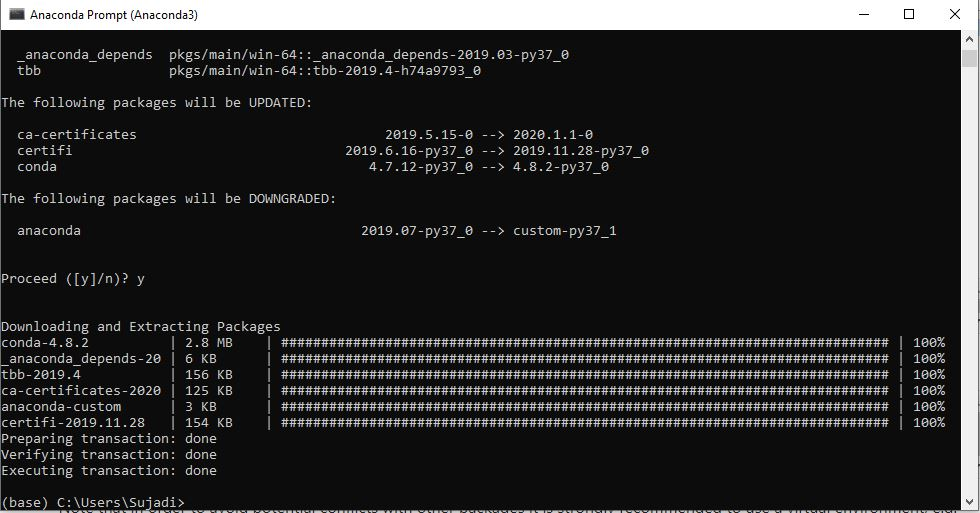
\includegraphics[scale=0.5]{figures/1174051/1/1.JPG}
\caption{Installasi}
\label{contoh}
\end{figure}
\begin{figure}[H]
\centering
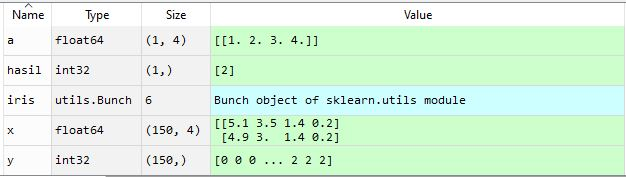
\includegraphics[width=4cm]{figures/1174051/1/2.JPG}
\caption{Isi Variabel Explorer}
\end{figure}
\item Mencoba loading an example dataset
\hfill\break
\lstinputlisting[firstline=8, lastline=12]{src/1174051/1/1174051.py}
\item Mencoba Learning dan predicting
\hfill\break
\lstinputlisting[firstline=14, lastline=24]{src/1174051/1/1174051.py}
\item Mencoba Model Persistence
\hfill\break
\lstinputlisting[firstline=26, lastline=36]{src/1174051/1/1174051.py}
\item Mencoba Conventions
\hfill\break
\lstinputlisting[firstline=38, lastline=50]{src/1174051/1/1174051.py}
\end{enumerate}
\subsection{Penanganan Error}
\begin{enumerate}
\item ScreenShoot Error
\begin{figure}[H]
	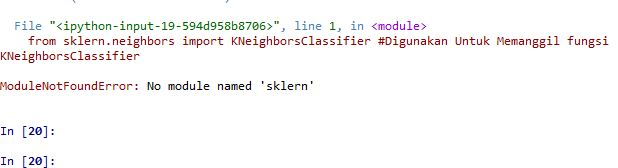
\includegraphics[width=4cm]{figures/1174051/1/error/1.JPG}
	\centering
	\caption{Import Error}
\end{figure}
\item Tuliskan Kode Error dan Jenis Error
\begin{itemize}
	\item ModuleNotFoundError
\end{itemize}
\item Cara Penangan Error
\begin{itemize}
	\item ModuleNotFoundError
	\hfill\break
	Typo pada pemanggilan sklearn
\end{itemize}
\end{enumerate}
\subsection{Bukti Tidak Plagiat}
\begin{figure}[H]
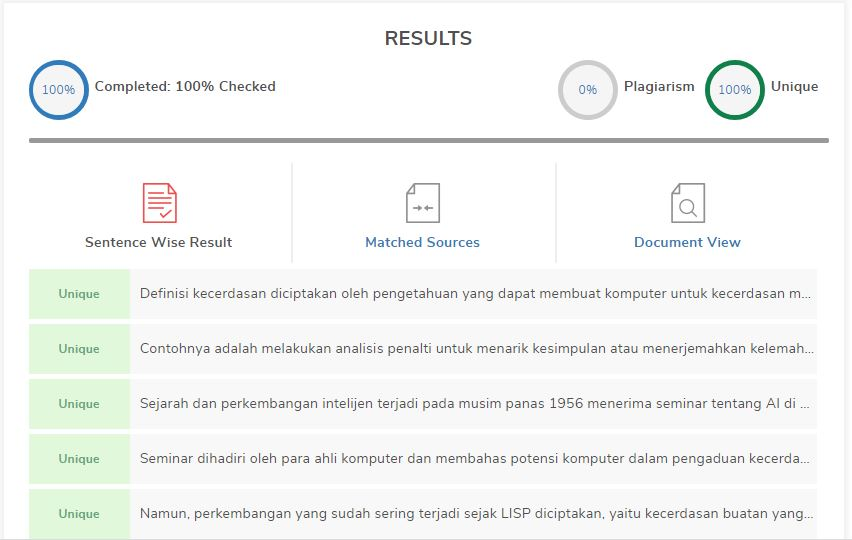
\includegraphics[width=4cm]{figures/1174051/1/plagiat/1.JPG}
\centering
\caption{Bukti Tidak Melakukan Plagiat 1}
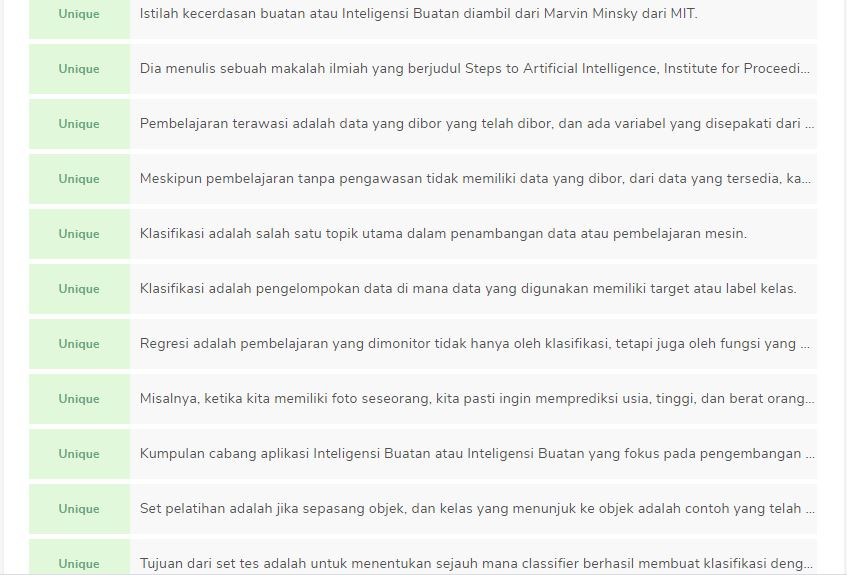
\includegraphics[width=4cm]{figures/1174051/1/plagiat/2.JPG}
\centering
\caption{Bukti Tidak Melakukan Plagiat 2}
\end{figure}
%\section{1174021 - Muhammad Fahmi}
\subsection{Teori}
\begin{enumerate}

	\item Defenisi Kecerdasan Buatan
	\hfill\break
	Kecerdasan buatan yang jika dalam bahasa inggris ialah Artificial Intelligence (AI) adalah bagian dari ilmu komputer. Dengan penelitian dan pengembangan kecerdasan buatan, ia berusaha untuk tidak hanya berhasil tetapi untuk melengkapi pemikiran manusia dengan program komputer belajar mandiri. AI juga sudah banyak di aplikasikan di dunia bisnis, misalnya, dalam Google Maps. dan Istilah dalam AI juga sudah tidak asing lagi yaitu "Neural Network" dan "Deep learning" yang terkait dengan pengembangan kecerdasan buatan.

	\begin{figure}[H]
	\centering
		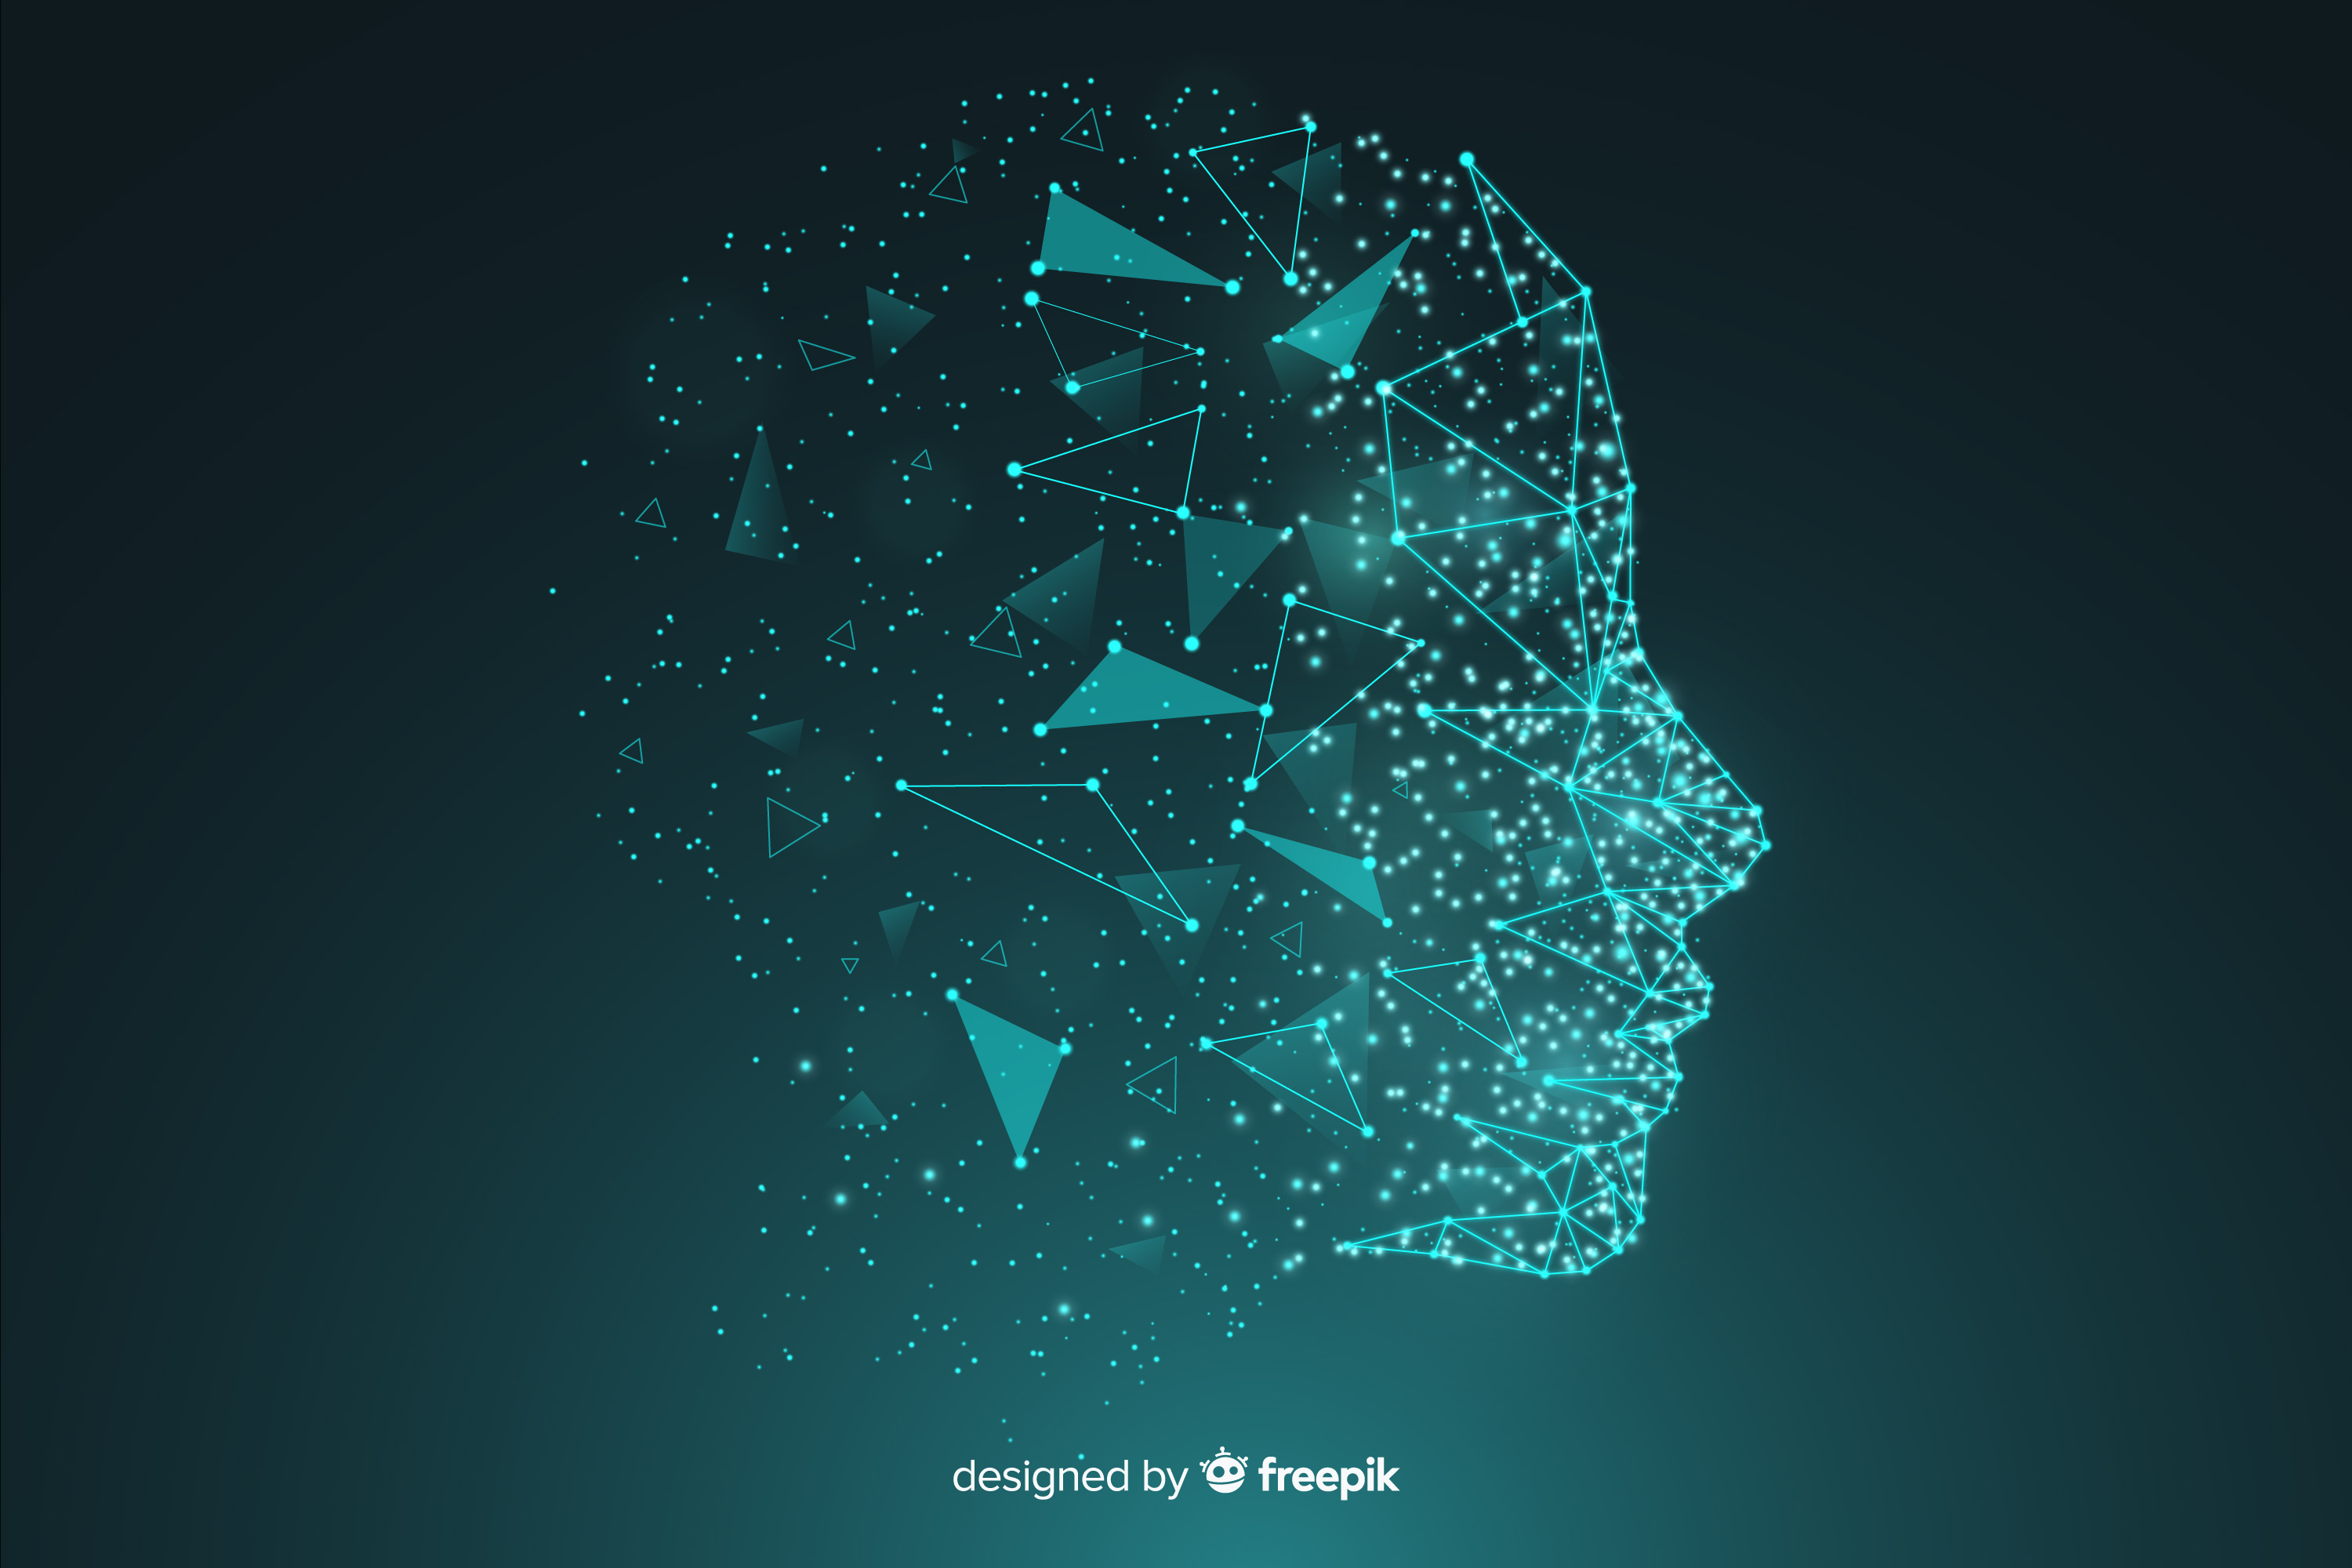
\includegraphics[width=4cm]{figures/1174021/tugas1/materi/1.jpg}
		\caption{Kecerdasan Buatan.}
	\end{figure}

	\item Sejarah dan Perkembangan
	\hfill\break
	Pada tahun 1950 yang bertempat di AS kecerdasan buatan atau AI itu dimulai pada konferensi ilmiah di Dartmouth, M. Minsky, J.McCarthy, A. Newell, dan HA Simon adalah yang pertama berbicara tentang "kecerdasan buatan." Definisi yang sering dikutip untuk kecerdasan buatan diberikan oleh salah satu pendiri subjek, Marvin Minsky, pada tahun 1966: "Kecerdasan Buatan adalah ilmu membuat mesin melakukan hal-hal yang membutuhkan kecerdasan jika dilakukan oleh manusia." Jadi, ditentukan bahwa kecerdasan buatan adalah ilmu dan kedua mesin dapat mengambil alih pekerjaan manusia yang membutuhkan kecerdasan manusia. Adapun mengapa AI yaitu untuk pemecah an masalah umum dari para peneliti Newell, Shaw, dan Simon pada tahun 1960-an. Penelitian ini dapat memecahkan masalah sederhana. Namun, hasil penelitian tersebut tidak dapat digeneralisasi. Pada akhir 1960-an, program lain ditulis dengan ELIZA. Dengan demikian, Joseph Weizenbaum, seorang peneliti MIT,simulasikan sesi terapi. Pada tahun-tahun berikutnya, sains muda terus dikembangkan, yang diproduksi oleh MYCIN pada awal 1970-an dalam sistem inovatif lain berbasis AI. MYCIN dapat membantu dokter mendiagnosis.
	

	\item Kecerdasan buatan terbagi atas beberapa metode yaitu:
	\hfill\break
	Supervised learning, Unsupervised Learning, Klasifikasi, Regresi, Dataset, Trainingset dan juga Testingset.
	\begin{itemize}
		\item Supervised Learning
		\hfill\break
		Sebuah algoritma pembelajaran mesin yang dapat menerapkan informasi yang sudah ada dalam data dengan memberikan label tertentu, misalnya data yang telah diklasifikasikan sebelumnya (diarahkan). Algoritma ini mampu memberikan target untuk output yang dilakukan dengan membandingkan pengalaman belajar masa yang sudah lampau.
		\item Unsupervised Learning 
		\hfill\break
		Berbeda dengan Supervised Learning, Unsupervised Learning ialah sebuah pembelajaran mesin tanpa pengawasan adalah pembelajaran mesin yang digunakan pada data yang tidak memiliki informasi yang dapat diterapkan secara langsung (tidak diarahkan). Algoritma ini diharapkan dapat menemukan struktur tersembunyi dalam data yang tidak berlabel.
		\item Klasifikasi
		\hfill\break
		Klasifikasi adalah sampel milik dua kelas atau lebih dan ingin belajar dari data yang sudah diberi label cara memprediksi kelas data yang tidak berlabel. Contoh masalah klasifikasi adalah pengenalan digit tulisan tangan, di mana tujuannya adalah untuk menetapkan masing-masing vektor input ke salah satu dari sejumlah kategori diskrit. 
		\item Regresi
		\hfill\break
		Regrasi ialah sebuah metode untuk mengembangkan model (persamaan) yang menjelaskan hubungan antara beberapa variabel. Output dari analisis regresi adalah persamaan regresi. Dalam model regresi variabel dibagi menjadi dua bagian, yaitu variabel respon atau yang biasa juga disebut variabel dependen dan variabel explanatory atau juga biasa disebut variabel prediktor atau disebut juga variabel independen.
		\item Data set
		\hfill\break
		Dataset adalah sebuah kumpulan data atau objek dan bagaimana relasi dalam memori. Struktur Dataset mirip dengan data di dalam database. Dataset berisi koleksi dari datatable maupun data relasi.
		\item Training Set
		\hfill\break
		Training set ialah bagian dari dataset yang berfungsi untuk membuat prediksi atau mengatur fungsi dari algoritma-algoritma yang ada. Fungsi nya yang lain juga ada sesuai tujuannya masing-masing. Trainingset memberikan instruksi melalui algoritma sehingga mesin dapat mengerti dan membuat kolerasi sendiri.		
		\item Testing Set
		\hfill\break
		Sama seperti training set, testing set juga bagian dari dataset yang berfungsi menguji untuk melihat akurasinya, atau bisa juga untuk melihat suatu kinerja atau performa.
	\end{itemize}
\end{enumerate}
\subsection{Praktek}
\begin{enumerate}
	\item Instalasi Library scikit dari Anaconda, mencoba kompilasi dan uji coba ambil contoh kode dan lihat variabel explorer
	\hfill\break
	\begin{figure}[H]
		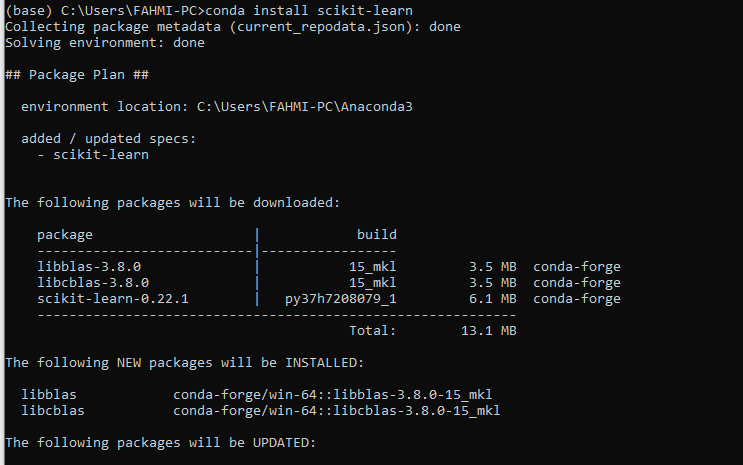
\includegraphics[width=4cm]{figures/1174021/tugas1/materi/2.PNG}
		\centering
		\caption{Instalasi Library Scikit Learn}
	\end{figure}
	\begin{figure}[H]
		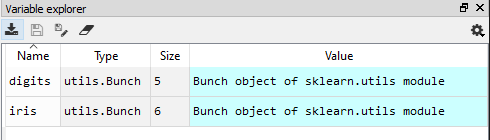
\includegraphics[width=4cm]{figures/1174021/tugas1/materi/3.PNG}
		\centering
		\caption{Isi Variabel Explorer}
	\end{figure}
	\item Uji coba loading an example dataset
	\hfill\break
	\lstinputlisting[firstline=10, lastline=14]{src/1174021/tugas1.py}
	\item Uji coba Learning dan predicting
	\hfill\break
	\lstinputlisting[firstline=18, lastline=21]{src/1174021/tugas1.py}
	\item Uji coba Model Persistence
	\hfill\break
	\lstinputlisting[firstline=25, lastline=41]{src/1174021/tugas1.py}
	\item Uji coba Conventions
	\hfill\break
	\lstinputlisting[firstline=44, lastline=56]{src/1174021/tugas1.py}
\end{enumerate}
\subsection{Penanganan Error}
\begin{enumerate}
	\item ScreenShoot Error
	\begin{figure}[H]
		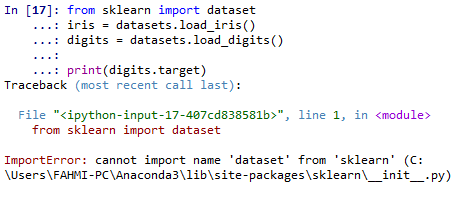
\includegraphics[width=4cm]{figures/1174021/tugas1/error/1.PNG}
		\centering
		\caption{Import Error}
	\end{figure}
	\begin{figure}[H]
		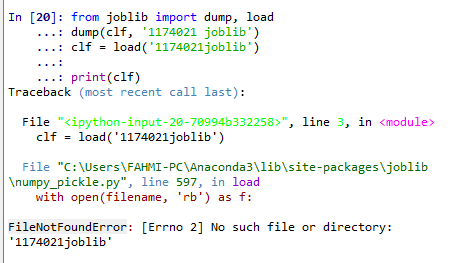
\includegraphics[width=4cm]{figures/1174021/tugas1/error/2.PNG}
		\centering
		\caption{FileNotFoundError}
	\end{figure}
	\item Tuliskan Kode Error dan Jenis Error
	\begin{itemize}
		\item Import Error
		\item FileNotFoundError
	\end{itemize}
	\item Cara Penangan Error
	\begin{itemize}
		\item Import Error
		\hfill\break
		Error terdapat typo pada dataset, seharusnya datasets
		\item FileNotFoundError
		\hfill\break
		Error terdapat pada 1174021joblib, tidak ada file yang dibaca, seharusnya 1174021.joblib
	\end{itemize}
\end{enumerate}
\subsection{Bukti Tidak Plagiat}
\begin{figure}[H]
	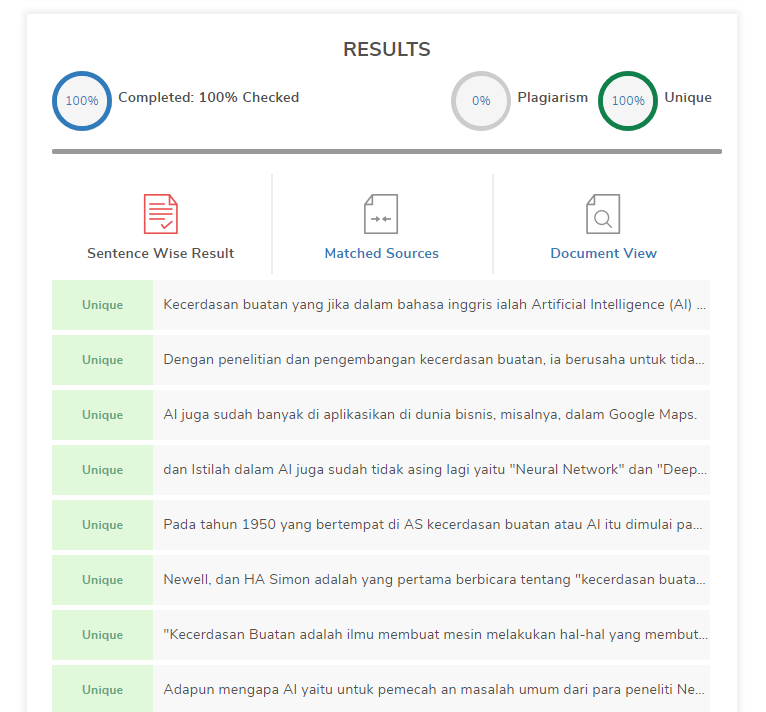
\includegraphics[width=4cm]{figures/1174021/tugas1/buktiplagiat/1.PNG}
	\centering
	\caption{Bukti Tidak Melakukan Plagiat Chapter 1}
\end{figure}
%\section{1174096 - Nico Ekklesia Sembiring}
\subsection{Teori}
\begin{enumerate}
	\item Pengetian, Sejarah dan Perkembangan Kecerdasan Buatan
	\hfill\break
    Kecerdasan buatan (Artificial Inteligence) merupakan suatu entitas yang cerdas secara ilmiah yang merupakan hasil dari gagasan dan ciptaan manusia. Suatu entitas dimasukkan kedalam suatu alat atau mesin sehingga membuat alat atau mesin itu dapat seolah-olah dapat berpikir dan mengambil keputusan sendiri. Kecerdasan buatan berbeda dengan perangkat computer, dimana computer melakukan pengambilan keputusan dan melakukan fungsi fungsi hanmya pada saat diarahkan oleh pengguna, tidak dapat melakukan secara otomatis. 
    \hfill\break
    Kecerdasan buatan dapat mengambil keputusan secara otomatis berdasarkan pengalaman yang telah sebelumnya terjadi dan direkam dan disimpan pada database perangkat kecerdasan buatan. Rekaman aktifitas yang telah dilakukan tersebut dapat diterapkan dikemudian hari ketika diperlukan. Kehadiran perangkat yang menggunakan kecerdasan buatan pada masa sekarang ini merupakan suatu kemajuan dalam bidang teknologi yang paling baik, dimana konsep perangkat yang menggunakan kecerdasan buatan sudah mulai dimanfaatkan dalam berbagai bidang seperti multimedia, mesin pencari, robotic, dan lain lain. 
    \hfill\break
    Komputer dapat dibuat menjadi entitas yang cerdas dengan menyediakan data dalam database. Selain diberi data, komputer juga dapat diberikan suatu kemampuan dalam mempelajari data. Pelatihan dan pembelajaran data ini akan membuat sistem dapat menentukan keputusan dan melakukan tugas untuk membuatnya lebih mudah bagi manusia di masa depan.
    \hfill\break
    Jarvis memiliki kemampuan berbicara memiliki kemampuan untuk mendeteksi kondisi kesehatan dan melakukan hal-hal lain yang diperintahkan oleh penciptanya. Ini disebabkan oleh kecerdasan Jarvis yang sudah sangat terlatih. Komputer pintar seperti jarvis diharapkan dapat ditemukan di masa depan sehingga banyak orang berlomba untuk mengembangkannya sekarang.
    \hfill\break


	Definisi kecerdasan buatan itu sendiri adalah suatu system teknologi yang didalamnya ditambahakan kecerdasan oleh manusia, kecerdasan buatan diatur dan dikembangkan dalam konteks ilmiah, dan bentukan dari kecerdasan entitas ilmiah yang ada.
	\item defenisi dari Supervised learning, klasifikasi, regresi, unsupervised learning, dataset, trainingset dan testingset.
	\begin{itemize}
		\item Supervised Learning
		\hfill\break
		Supervised Learning merupakan sebuah tipe learning yang mempunyai variable input dan variable output, tipe ini juga menggunakan satu algoritma atau lebih dari satu algoritma yang digunakan untuk mempelajari fungsi  pemetaan dari input ke output.
		\item Klasifikasi
		\hfill\break
		Klasifikasi adalah pengelompokan data di mana data yang digunakan memiliki label atau kelas target. Sehingga algoritma untuk menyelesaikan masalah klasifikasi dikategorikan ke dalam pembelajaran terbimbing.
		\item Regresi
		\hfill\break
		regressi metode analisis statistik yang digunakan untuk dapat melihat efek antara dua atau lebih variabel. Hubungan variabel dalam pertanyaan adalah fungsional yang diwujudkan dalam bentuk model matematika. Dalam analisis regresi, variabel dibagi menjadi dua jenis, yaitu variabel respons atau yang biasa disebut variabel dependen dan variabel independen atau dikenal sebagai variabel independen. Ada beberapa jenis analisis regresi, yaitu regresi sederhana yang mencakup linear sederhana dan regresi non-linear sederhana dan regresi berganda yang mencakup banyak linier atau non-linear berganda. Analisis regresi digunakan dalam pembelajaran mesin pembelajaran dengan metode pembelajaran terawasi.
		\item Unsupervised learning 
		\hfill\break
		unsupervised learning jenis pembelajaran di mana kita hanya memiliki data input (input data) tetapi tidak ada variabel output yang terkait. Tujuan dari pembelajaran tanpa pengawasan adalah untuk memodelkan struktur dasar atau distribusi data dengan tujuan mempelajari data lebih lanjut, dengan kata lain, itu adalah fungsi simpulan yang menggambarkan atau menjelaskan data.
		\item Data set
		\hfill\break
		Data set objek yang merepresentasikan data dan relasinya di memory. Strukturnya mirip dengan data di database. Dataset berisi koleksi dari datatable dan datarelation.
		\item Training Set
		\hfill\break
		Training set adalah bagian dari dataset yang di latih untuk membuat prediksi atau menjalankan fungsi dari algoritma ML lain sesuai dengan masing-masing. Memberikan instruksi melalui algoritma sehingga mesin yang di praktikkan dapat menemukan korelasinya sendiri.
		\item Testing Set
		\hfill\break
		testing set adalah bagian dari dataset yang kami uji untuk melihat akurasinya, atau dengan kata lain untuk melihat kinerjanya.
	\end{itemize}
\end{enumerate}
\subsection{Praktek}
\begin{enumerate}
	\item Instalasi Library scikit dari ianaconda, mencoba kompilasi dan uji coba ambil contoh kode dan lihat variabel explorer
    \hfill\break
    \begin{itemize}
		\item buka Anaconda Prompt
		\hfill\break
		\item Ketikkan conda install scikit-learn
		\begin{figure}[H]
            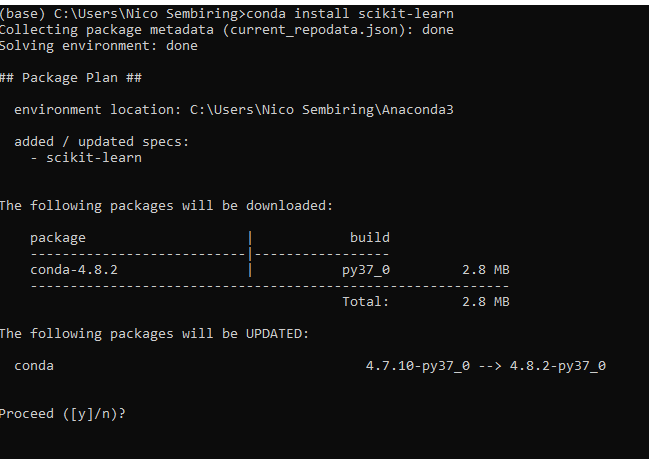
\includegraphics[width=4cm]{figures/1174096/1/install1.PNG}
            \centering
            \caption{Instalasi Package Scikit Learn}
        \end{figure}
		\hfill\break
		Klasifikasi adalah pengelompokan data di mana data yang digunakan memiliki label atau kelas target. Sehingga algoritma untuk menyelesaikan masalah klasifikasi dikategorikan ke dalam pembelajaran terbimbing.
		\item Kemudian pilih Y
		\begin{figure}[H]
            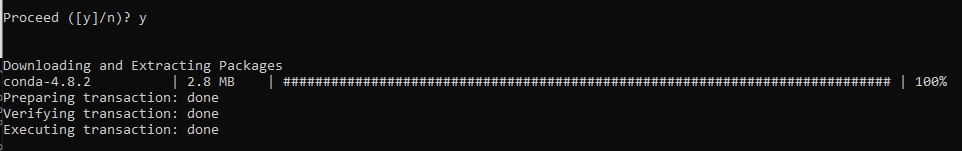
\includegraphics[width=4cm]{figures/1174096/1/install2.PNG}
            \centering
            \caption{pilih y}
        \end{figure}
	\end{itemize}
	
	\item Mencoba loading an example dataset
	\hfill\break
	\lstinputlisting[firstline=8, lastline=12]{src/1174096/1/1174096.py}
	\item Mencoba Learning dan predicting
	\hfill\break
	\lstinputlisting[firstline=14, lastline=24]{src/1174096/1/1174096.py}
	\item Mencoba Model Persistence
	\hfill\break
	\lstinputlisting[firstline=26, lastline=36]{src/1174096/1/1174096.py}
	\item Mencoba Conventions
	\hfill\break
	\lstinputlisting[firstline=38, lastline=56]{src/1174096/1/1174096.py}
\end{enumerate}
\subsection{Penanganan Error}
\begin{enumerate}
	\item ScreenShoot Error
	\begin{figure}[H]
		\includegraphics[width=4cm]{figures/1174096/error/1_import.png}
		\centering
		\caption{Import Error}
	\end{figure}
	\begin{figure}[H]
		\includegraphics[width=4cm]{figures/1174096/error/1_value.png}
		\centering
		\caption{Value Error}
	\end{figure}
	\item Tuliskan Kode Error dan Jenis Error
	\begin{itemize}
		\item Import Error
		\item Value Error
	\end{itemize}
	\item Cara Penangan Error
	\begin{itemize}
		\item Import Error
		\hfill\break
		Dengan Menginstall Library Yang Tidak Ditemukan
		\item Value Error
		\hfill\break
		Mengubah Bentuk Arraynya, Menjadi 1 Dimensi
	\end{itemize}
\end{enumerate}
\subsection{Bukti Tidak Plagiat}
\begin{figure}[H]
	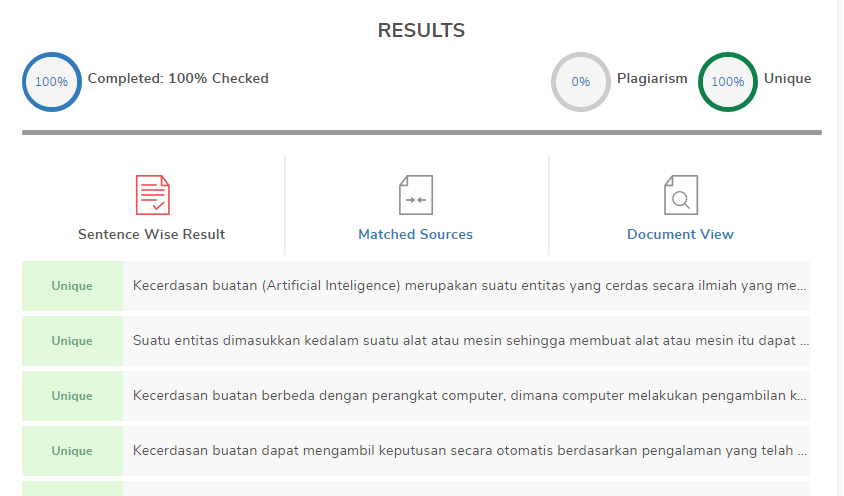
\includegraphics[width=4cm]{figures/1174096/bukti/plagiarisme.PNG}
	\centering
	\caption{Bukti Tidak Plagiarisme}
\end{figure}
%\section{1174012 - Damara Benedikta }
\subsection{Teori}
\begin{enumerate}
	\item Sejarah dan Perkembangan
	\hfill\break
	Kecerdasan Buatan atau dalam Bahasa inggris sering disebut Artifical Intelligence yang sering disebut juga sebagai AI, pada 10 tahun lalu masyarakat belum terlalu mengetahui hal tersebut dan masih menjadi bahan candaan dikalangan masyarakat. Awal perkembangan AI dimulai pada tahun 1952-1969 yang dimulai dengan kesuksesan Newwll dan temannya simon menggunakan sebuah program yang disebut dengan General Problem Solver. Program ini dibangun untuk tujuan penyelesaiin masalah secara manusiawi. Pada tahun 1966-1974 perkembangan kecerdasan buatan mulai melambat. Ada 3 faktor utama yang menyebabkan hal itu terjadi:
	\begin{itemize}
		\item Banyak subjek pada program AI yang bermunculan hanya mengandung sedikit atau bahkan sama sekali tidak  mengandung sama sekali pengetahuan (knowledge).
		\item Kecerdasan buatan harus bisa menyelesaikan banyak masalah.
		\item Untuk menghasilkan perilkau intelijensia ada beberapa batasan pada struktur yang bisa digunakan.
	\end{itemize}
	Definisi AI (Artificial Intelligence) atau kecerdasan buatan merupakan sebuah kecerdasan yang ditambahkan kepada sebuah system yang dapat diatur. Atau juga dapat didefinisikan kemampuan sebuah system untuk dapat menafsirkan data dengan benar untuk dapat mencapai sebuah tujuan dan tugas tertentu sehingga mesin dapat bekerja secara fleksibel seperti manusia.
	\item Definisi
	\hfill\break
	Supervised learning, klasifikasi, regresi, unsupervised learning, dataset, trainingset dan testingset.
	\begin{itemize}
		\item Supervised Learning
		\hfill\break
		Supervised Learning merupakan sebuah tipe learning yang mempunyai variable input dan variable output, tipe ini juga menggunakan satu algoritma atau lebih dari satu algoritma yang digunakan untuk mempelajari fungsi  pemetaan dari input ke output.
		\item Klasifikasi
		\hfill\break
		Klasifikasi adalah pengelompokan data di mana data yang digunakan memiliki label atau kelas target. Sehingga algoritma untuk menyelesaikan masalah klasifikasi dikategorikan ke dalam pembelajaran terbimbing.
		\item Regresi
		\hfill\break
		regressi metode analisis statistik yang digunakan untuk dapat melihat efek antara dua atau lebih variabel. Hubungan variabel dalam pertanyaan adalah fungsional yang diwujudkan dalam bentuk model matematika. Dalam analisis regresi, variabel dibagi menjadi dua jenis, yaitu variabel respons atau yang biasa disebut variabel dependen dan variabel independen atau dikenal sebagai variabel independen. Ada beberapa jenis analisis regresi, yaitu regresi sederhana yang mencakup linear sederhana dan regresi non-linear sederhana dan regresi berganda yang mencakup banyak linier atau non-linear berganda. Analisis regresi digunakan dalam pembelajaran mesin pembelajaran dengan metode pembelajaran terawasi.
		\item Unsupervised learning 
		\hfill\break
		unsupervised learning jenis pembelajaran di mana kita hanya memiliki data input (input data) tetapi tidak ada variabel output yang terkait. Tujuan dari pembelajaran tanpa pengawasan adalah untuk memodelkan struktur dasar atau distribusi data dengan tujuan mempelajari data lebih lanjut, dengan kata lain, itu adalah fungsi simpulan yang menggambarkan atau menjelaskan data.
		\item Data set
		\hfill\break
		Data set objek yang merepresentasikan data dan relasinya di memory. Strukturnya mirip dengan data di database. Dataset berisi koleksi dari datatable dan datarelation.
		\item Training Set
		\hfill\break
		Training set merupakan bagian dari dataset yang di latih untuk membuat prediksi atau menjalankan fungsi dari algoritma ML lain sesuai dengan masing-masing. Memberikan instruksi melalui algoritma sehingga mesin yang di praktikkan dapat menemukan korelasinya sendiri.
		\item Testing Set
		\hfill\break
		testing set adalah bagian dari dataset yang kami uji untuk melihat akurasinya, atau dengan kata lain untuk melihat kinerjanya.
	\end{itemize}
\end{enumerate}
\subsection{Praktek}
\begin{enumerate}
	\item Instalasi Library scikit dari ianaconda, mencoba kompilasi dan uji coba ambil contoh kode dan lihat variabel explorer
	\hfill\break
	\begin{figure}[H]
		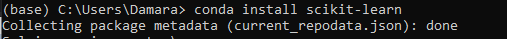
\includegraphics[width=4cm]{figures/1174012/1/ins1.PNG}
		\centering
		\caption{Instalasi Package Scikit Learn}
	\end{figure}
    \begin{figure}[H]
		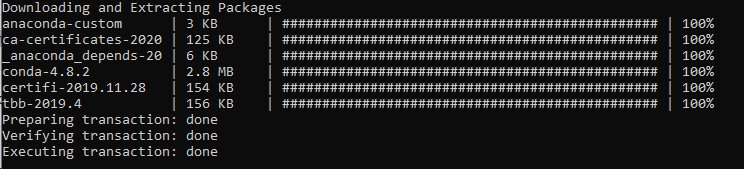
\includegraphics[width=4cm]{figures/1174012/1/ins2.PNG}
		\centering
		\caption{Instalasi Package Scikit Learn}
	\end{figure}
	\begin{figure}[H]
		\includegraphics[width=4cm]{figures/1174012/1/variabel.png}
		\centering
		\caption{Isi Variabel Explorer}
	\end{figure}
	\item Mencoba loading an example dataset
	\hfill\break
	\lstinputlisting[firstline=1, lastline=5]{src/1174012/1/1174012.py}
	\item Mencoba Learning dan predicting
	\hfill\break
	\lstinputlisting[firstline=7, lastline=18]{src/1174012/1/1174012.py}
	\item Mencoba Model Persistence
	\hfill\break
	\lstinputlisting[firstline=19, lastline=25]{src/1174012/1/1174012.py}
	\item Mencoba Conventions
	\hfill\break
	\lstinputlisting[firstline=31, lastline=43]{src/1174012/1/1174012.py}
\end{enumerate}
\subsection{Penanganan Error}
\begin{enumerate}
	\item ScreenShoot Error
	\begin{figure}[H]
		\includegraphics[width=4cm]{figures/1174012/error/1.png}
		\centering
		\caption{Import Error}
	\end{figure}
	\begin{figure}[H]
		\includegraphics[width=4cm]{figures/1174012/error/2.png}
		\centering
		\caption{Value Error}
	\end{figure}
	\item Tuliskan Kode Error dan Jenis Error
	\begin{itemize}
		\item Import Error
		\item Value Error
	\end{itemize}
	\item Cara Penangan Error
	\begin{itemize}
		\item Import Error
		\hfill\break
		Dengan Menginstall Library Yang Tidak Ditemukan
		\item Value Error
		\hfill\break
		Mengubah Bentuk Arraynya, Menjadi 1 Dimensi
	\end{itemize}
\end{enumerate}
\subsection{Bukti Tidak Plagiat}
\begin{figure}[H]
	\includegraphics[width=4cm]{figures/1174012/plagiat/plagiat.PNG}
	\centering
	\caption{Bukti Tidak Melakukan Plagiat Chapter 1}
\end{figure}
%\section{1174095 - Muhammad Dzihan Al-Bannai}
\subsection{Teori}
\begin{enumerate}

	\item Defenisi Kecerdasan Buatan
	\hfill\break
	Kecerdasan buatan yang jika dalam bahasa inggris ialah Artificial Intelligence (AI) adalah bagian dari ilmu komputer. Dengan penelitian dan pengembangan kecerdasan buatan, ia berusaha untuk tidak hanya berhasil tetapi untuk melengkapi pemikiran manusia dengan program komputer belajar mandiri. AI juga sudah banyak di aplikasikan di dunia bisnis, misalnya, dalam Google Maps. dan Istilah dalam AI juga sudah tidak asing lagi yaitu "Neural Network" dan "Deep learning" yang terkait dengan pengembangan kecerdasan buatan.



	\item Sejarah dan Perkembangan
	\hfill\break
	Pada tahun 1950 yang bertempat di AS kecerdasan buatan atau AI itu dimulai pada konferensi ilmiah di Dartmouth, M. Minsky, J.McCarthy, A. Newell, dan HA Simon adalah yang pertama berbicara tentang "kecerdasan buatan." Definisi yang sering dikutip untuk kecerdasan buatan diberikan oleh salah satu pendiri subjek, Marvin Minsky, pada tahun 1966: "Kecerdasan Buatan adalah ilmu membuat mesin melakukan hal-hal yang membutuhkan kecerdasan jika dilakukan oleh manusia." Jadi, ditentukan bahwa kecerdasan buatan adalah ilmu dan kedua mesin dapat mengambil alih pekerjaan manusia yang membutuhkan kecerdasan manusia. Adapun mengapa AI yaitu untuk pemecah an masalah umum dari para peneliti Newell, Shaw, dan Simon pada tahun 1960-an. Penelitian ini dapat memecahkan masalah sederhana. Namun, hasil penelitian tersebut tidak dapat digeneralisasi. Pada akhir 1960-an, program lain ditulis dengan ELIZA. Dengan demikian, Joseph Weizenbaum, seorang peneliti MIT,simulasikan sesi terapi. Pada tahun-tahun berikutnya, sains muda terus dikembangkan, yang diproduksi oleh MYCIN pada awal 1970-an dalam sistem inovatif lain berbasis AI. MYCIN dapat membantu dokter mendiagnosis.
	

	\item Kecerdasan buatan terbagi atas beberapa metode yaitu:
	\hfill\break
	Supervised learning, Unsupervised Learning, Klasifikasi, Regresi, Dataset, Trainingset dan juga Testingset.
	\begin{itemize}
		\item Supervised Learning
		\hfill\break
		Sebuah algoritma pembelajaran mesin yang dapat menerapkan informasi yang sudah ada dalam data dengan memberikan label tertentu, misalnya data yang telah diklasifikasikan sebelumnya (diarahkan). Algoritma ini mampu memberikan target untuk output yang dilakukan dengan membandingkan pengalaman belajar masa yang sudah lampau.
		\item Unsupervised Learning 
		\hfill\break
		Berbeda dengan Supervised Learning, Unsupervised Learning ialah sebuah pembelajaran mesin tanpa pengawasan adalah pembelajaran mesin yang digunakan pada data yang tidak memiliki informasi yang dapat diterapkan secara langsung (tidak diarahkan). Algoritma ini diharapkan dapat menemukan struktur tersembunyi dalam data yang tidak berlabel.
		\item Klasifikasi
		\hfill\break
		Klasifikasi adalah sampel milik dua kelas atau lebih dan ingin belajar dari data yang sudah diberi label cara memprediksi kelas data yang tidak berlabel. Contoh masalah klasifikasi adalah pengenalan digit tulisan tangan, di mana tujuannya adalah untuk menetapkan masing-masing vektor input ke salah satu dari sejumlah kategori diskrit. 
		\item Regresi
		\hfill\break
		Regrasi ialah sebuah metode untuk mengembangkan model (persamaan) yang menjelaskan hubungan antara beberapa variabel. Output dari analisis regresi adalah persamaan regresi. Dalam model regresi variabel dibagi menjadi dua bagian, yaitu variabel respon atau yang biasa juga disebut variabel dependen dan variabel explanatory atau juga biasa disebut variabel prediktor atau disebut juga variabel independen.
		\item Data set
		\hfill\break
		Dataset adalah sebuah kumpulan data atau objek dan bagaimana relasi dalam memori. Struktur Dataset mirip dengan data di dalam database. Dataset berisi koleksi dari datatable maupun data relasi.
		\item Training Set
		\hfill\break
		Training set ialah bagian dari dataset yang berfungsi untuk membuat prediksi atau mengatur fungsi dari algoritma-algoritma yang ada. Fungsi nya yang lain juga ada sesuai tujuannya masing-masing. Trainingset memberikan instruksi melalui algoritma sehingga mesin dapat mengerti dan membuat kolerasi sendiri.		
		\item Testing Set
		\hfill\break
		Sama seperti training set, testing set juga bagian dari dataset yang berfungsi menguji untuk melihat akurasinya, atau bisa juga untuk melihat suatu kinerja atau performa.
	\end{itemize}
\end{enumerate}
\subsection{Praktek}
\begin{enumerate}
	\item Instalasi Library scikit dari Anaconda, mencoba kompilasi dan uji coba ambil contoh kode dan lihat variabel explorer
	\hfill\break
	\begin{figure}[H]
		\includegraphics[width=4cm]{figures/1174095/tugas1/materi/1.PNG}
		\centering
		\caption{Instalasi Library Scikit Learn}
	\end{figure}
	\begin{figure}[H]
		\includegraphics[width=4cm]{figures/1174095/tugas1/materi/2.PNG}
		\centering
		\caption{Isi Variabel Explorer}
	\end{figure}
	\item Uji coba loading an example dataset
	\hfill\break
	\lstinputlisting[firstline=10, lastline=14]{src/1174095/tugas1.py}
	\item Uji coba Learning dan predicting
	\hfill\break
	\lstinputlisting[firstline=18, lastline=21]{src/1174095/tugas1.py}
	\item Uji coba Model Persistence
	\hfill\break
	\lstinputlisting[firstline=25, lastline=41]{src/1174095/tugas1.py}
	\item Uji coba Conventions
	\hfill\break
	\lstinputlisting[firstline=44, lastline=56]{src/1174095/tugas1.py}
\end{enumerate}
\subsection{Penanganan Error}
\begin{enumerate}
	\item ScreenShoot Error
	\begin{figure}[H]
		\includegraphics[width=4cm]{figures/1174095/tugas1/error/1.PNG}
		\centering
		\caption{Import Error}
	\end{figure}
	\begin{figure}[H]
		\includegraphics[width=4cm]{figures/1174095/tugas1/error/2.PNG}
		\centering
		\caption{FileNotFoundError}
	\end{figure}
	\item Tuliskan Kode Error dan Jenis Error
	\begin{itemize}
		\item Import Error
		\item FileNotFoundError
	\end{itemize}
	\item Cara Penangan Error
	\begin{itemize}
		\item Import Error
		\hfill\break
		Kesalahan pemanggilan pada import dapat menghasilkan error, seperti pada pemanggilan datasets, pastikan kembali pemanggilannya sesuai.
		\item FileNotFoundError
		\hfill\break
		Perhatikan format file pada joblib, format harus memakai titik terlebih dahulu.
	\end{itemize}
\end{enumerate}
\subsection{Bukti Tidak Plagiat}
\begin{figure}[H]
	\includegraphics[width=4cm]{figures/1174095/tugas1/buktiplagiat/plag.PNG}
	\centering
	\caption{Bukti Tidak Melakukan Plagiat Chapter 1}
\end{figure}
%\section{1174009 - Dwi Yulianingsih}
\subsection{Teori}
\begin{enumerate}
	\item Sejarah dan Perkembangan
	\hfill\break
	Kecerdasan Buatan atau dalam Bahasa inggris sering disebut Artifical Intelligence yang sering disebut juga sebagai AI, pada 10 tahun lalu masyarakat belum terlalu mengetahui hal tersebut dan masih menjadi bahan candaan dikalangan masyarakat. Awal perkembangan AI dimulai pada tahun 1952-1969 yang dimulai dengan kesuksesan Newwll dan temannya simon menggunakan sebuah program yang disebut dengan General Problem Solver. Program ini dibangun untuk tujuan penyelesaiin masalah secara manusiawi. Pada tahun 1966-1974 perkembangan kecerdasan buatan mulai melambat. Ada 3 faktor utama yang menyebabkan hal itu terjadi:
	\begin{itemize}
		\item Banyak subjek pada program AI yang bermunculan hanya mengandung sedikit atau bahkan sama sekali tidak  mengandung sama sekali pengetahuan (knowledge).
		\item Kecerdasan buatan harus bisa menyelesaikan banyak masalah.
		\item Untuk menghasilkan perilkau intelijensia ada beberapa batasan pada struktur yang bisa digunakan.
	\end{itemize}
	Definisi kecerdasan buatan itu sendiri adalah suatu system teknologi yang didalamnya ditambahakan kecerdasan oleh manusia, kecerdasan buatan diatur dan dikembangkan dalam konteks ilmiah, dan bentukan dari kecerdasan entitas ilmiah yang ada.
	\item Definisi
	\hfill\break
	Supervised learning, klasifikasi, regresi, unsupervised learning, dataset, trainingset dan testingset.
	\begin{itemize}
		\item Supervised Learning
		\hfill\break
		Supervised Learning merupakan sebuah tipe learning yang mempunyai variable input dan variable output, tipe ini juga menggunakan satu algoritma atau lebih dari satu algoritma yang digunakan untuk mempelajari fungsi  pemetaan dari input ke output.
		\item Klasifikasi
		\hfill\break
		Klasifikasi adalah pengelompokan data di mana data yang digunakan memiliki label atau kelas target. Sehingga algoritma untuk menyelesaikan masalah klasifikasi dikategorikan ke dalam pembelajaran terbimbing.
		\item Regresi
		\hfill\break
		regressi metode analisis statistik yang digunakan untuk dapat melihat efek antara dua atau lebih variabel. Hubungan variabel dalam pertanyaan adalah fungsional yang diwujudkan dalam bentuk model matematika. Dalam analisis regresi, variabel dibagi menjadi dua jenis, yaitu variabel respons atau yang biasa disebut variabel dependen dan variabel independen atau dikenal sebagai variabel independen. Ada beberapa jenis analisis regresi, yaitu regresi sederhana yang mencakup linear sederhana dan regresi non-linear sederhana dan regresi berganda yang mencakup banyak linier atau non-linear berganda. Analisis regresi digunakan dalam pembelajaran mesin pembelajaran dengan metode pembelajaran terawasi.
		\item Unsupervised learning 
		\hfill\break
		unsupervised learning jenis pembelajaran di mana kita hanya memiliki data input (input data) tetapi tidak ada variabel output yang terkait. Tujuan dari pembelajaran tanpa pengawasan adalah untuk memodelkan struktur dasar atau distribusi data dengan tujuan mempelajari data lebih lanjut, dengan kata lain, itu adalah fungsi simpulan yang menggambarkan atau menjelaskan data.
		\item Data set
		\hfill\break
		Data set objek yang merepresentasikan data dan relasinya di memory. Strukturnya mirip dengan data di database. Dataset berisi koleksi dari datatable dan datarelation.
		\item Training Set
		\hfill\break
		Training set adalah bagian dari dataset yang di latih untuk membuat prediksi atau menjalankan fungsi dari algoritma ML lain sesuai dengan masing-masing. Memberikan instruksi melalui algoritma sehingga mesin yang di praktikkan dapat menemukan korelasinya sendiri.
		\item Testing Set
		\hfill\break
		testing set adalah bagian dari dataset yang kami uji untuk melihat akurasinya, atau dengan kata lain untuk melihat kinerjanya.
	\end{itemize}
\end{enumerate}
\subsection{Praktek}
\begin{enumerate}
	\item Instalasi Library scikit dari ianaconda, mencoba kompilasi dan uji coba ambil contoh kode dan lihat variabel explorer
	\hfill\break
	\begin{figure}[H]
		\includegraphics[width=4cm]{figures/1174009/materi/1.png}
		\centering
		\caption{Instalasi Package Scikit Learn}
	\end{figure}
	\begin{figure}[H]
		\includegraphics[width=4cm]{figures/1174009/materi/2.PNG}
		\centering
		\caption{Isi Variabel Explorer}
	\end{figure}
	\item Mencoba loading an example dataset
	\hfill\break
	\lstinputlisting[firstline=7, lastline=11]{src/1174009/tugas1.py}
	\item Mencoba Learning dan predicting
	\hfill\break
	\lstinputlisting[firstline=13, lastline=22]{src/1174009/tugas1.py}
	\item Mencoba Model Persistence
	\hfill\break
	\lstinputlisting[firstline=25, lastline=34]{src/1174009/tugas1.py}
	\item Mencoba Conventions
	\hfill\break
	\lstinputlisting[firstline=37, lastline=48]{src/1174009/tugas1.py}
\end{enumerate}
\subsection{Penanganan Error}
\begin{enumerate}
	\item ScreenShoot Error
	\begin{figure}[H]
		\includegraphics[width=4cm]{figures/1174009/error/3.PNG}
		\centering
		\caption{Import Error}
	\end{figure}
	\begin{figure}[H]
		\includegraphics[width=4cm]{figures/1174009/error/4.PNG}
		\centering
		\caption{Value Error}
	\end{figure}
	\item Tuliskan Kode Error dan Jenis Error
	\begin{itemize}
		\item Import Error
		\item Value Error
	\end{itemize}
	\item Cara Penangan Error
	\begin{itemize}
		\item Import Error
		\hfill\break
		Dengan Menginstall Library Yang Tidak Ditemukan
		\item Value Error
		\hfill\break
		Mengubah Bentuk Arraynya, Menjadi 1 Dimensi
	\end{itemize}
\end{enumerate}
\subsection{Bukti Tidak Plagiat}
\begin{figure}[H]
	\includegraphics[width=4cm]{figures/1174009/buktiplagiat/1.png}
	\centering
	\caption{Bukti Tidak Melakukan Plagiat Chapter 1}
\end{figure}
%\section{1174008 - Arjun Yuda Firwanda}
\subsection{Teori}
\begin{enumerate}
	\item Definisi Kecerdasan Buatan
	\hfill\break
	Definisi Kecerdasan Buatan (Artificial Intelligence) yakni sebagai kecerdasan entitas ilmiah. Kecerdasan Buatan diciptakan dalam suatu mesin komputer agar dapat melakukan pekerjaan seperti halnya yang dilakukan manusia.
	
	\item Sejarah dan Perkembangan Kecerdasan Buatan
	\hfill\break
	Sejarah dan Kecerdasan Buatan tidak lepas dari sosok John McCarthy. Ia sebagai "Bapak AI".

	\begin{itemize}
		\item Cikal bakal kecerdasan buatan (tahun 1943 - 1955)
		
		\item Kelahiran Kecerdasan Buatan (tahun 1956)
		
		\item Awal kecerdasan buatan merupakan tahap pengembangan aplikasi AI yang sukses dibandingkan dengan program komputer (tahun 1952 - 1969)
		
		\item Kecerdasan Buatan menjadi industry  (tahun 1980 - sekarang)
		
		\item Kecerdasan Buatan menjadi disiplin ilmu (tahun 1987 - sekarang)
		
		\item Kecerdasan Buatan menampakkan diri di semua bidang (tahun 1995 - sekarang)

	\end{itemize}

	\item Definisi Supervised Learning
	\hfill\break
	Supervised Learning merupakan pembelajaran yang ada supervisornya. Maksudnya adalah label di tiap data nya. Label maksudnya merupakan sebuatan tag dari data yang ditambahkan dalam machine learning model.
	
	\item Regresi
	\hfill\break
	Regresi merupakan menebak nilai output dari nilai input yang diberikan, berdasarkan pola input - ouput sebelumnya.

	\item Klasifikasi
	\hfill\break
	Klasifikasi, merupakan mengetahui jenis kelamin siswa dari tinggi dan berat badannya.

	\item Definisi Unsupervised Learning
	\hfill\break
	Unsupervised learning memiliki keunggulan. Jika unsupervised learning memiliki label sebagai dasar prediksi baik serta membuat clasification dan regression algorithm K-Means, Hierarchical Clustering, DBSCAN, Fuzzy C-Means, Self-Organizing Map.

	\item Data Set
	\hfill\break
	Data Set, merupakan objek yang merepresentasikan data dan relasinya. Strukturnya mirip dengan data di database. Dataset berisi koleksi dari datatable dan datarelation.

	\item Trainning Set
	\hfill\break
	Trainning Set, merupakan konteks machine learning Training = latihan.

	\item Testing Set
	\hfill\break
	Testing Set, merupakan melakukan evaluasi terhadap performa algoritma tersebut. Pada proses testing ini, dilakukan untuk mwengetahui performa algoritma akan diuji menggunakan testing set, dimana testing set dan training set merupakan data yang berbeda.

\end{enumerate}


\subsection{Praktek}
\begin{enumerate}
	\item Instalasi Library scikit dari ianaconda, mencoba kompilasi dan uji coba ambil contoh kode dan lihat variabel explorer
	\hfill\break
	\begin{figure}[H]
		\includegraphics[width=4cm]{figures/1174008/1/instalasi.PNG}
		\centering
		\caption{Instalasi Package Scikit Learn}
	\end{figure}
	\begin{figure}[H]
		\includegraphics[width=4cm]{figures/1174008/1/variable.PNG}
		\centering
		\caption{Isi Variabel Explorer}
	\end{figure}

	\item Mencoba loading an example dataset
	\hfill\break
	\lstinputlisting[firstline=7, lastline=11]{src/1174008/1/1174008.py}

	\item Mencoba Learning dan predicting
	\hfill\break
	\lstinputlisting[firstline=13, lastline=22]{src/1174008/1/1174008.py}

	\item Mencoba Model Persistence
	\hfill\break
	\lstinputlisting[firstline=25, lastline=34]{src/1174008/1/1174008.py}

	\item Mencoba Conventions
	\hfill\break
	\lstinputlisting[firstline=37, lastline=48]{src/1174008/1/1174008.py}
\end{enumerate}

\subsection{Penanganan Error}
\begin{enumerate}
	\item ScreenShoot Error
	\begin{figure}[H]
		\includegraphics[width=4cm]{figures/1174008/error/error.PNG}
		\centering
		\caption{ Error Joblib}
	\end{figure}

	\item Tuliskan Kode Error dan Jenis Error
	\begin{itemize}
		\item Import Error
		\item Value Error
	\end{itemize}

	\item Cara Penangan Error
	\begin{itemize}
		\item Import Error
		\hfill\break
		Dengan Menginstall Library Yang Tidak Ditemukan
		\item Value Error
		\hfill\break
		Mengubah Bentuk Arraynya, Menjadi 1 Dimensi
	\end{itemize}
\end{enumerate}

\subsection{Bukti Tidak Plagiat}
\begin{figure}[H]
	\includegraphics[width=4cm]{figures/1174008/bukti/CekPlagiarisme.PNG}
	\centering
	\caption{Bukti Tidak Melakukan Plagiat Chapter 1}
\end{figure}
%\section{1174005 - Oniwaldus Bere Mali}
\subsection{Teori}
\begin{enumerate}

\item Sejarah dan Perkembangan
	\hfill\break
	Definisi kecerdasan buatan (AI) Kecerdasan buatan (Bahasa Inggris: kecerdasan buatan atau AI) didefinisikan sebagai kecerdasan entitas ilmiah. Sistem ini umumnya dianggap komputer. Kecerdasan dibuat dan ditempatkan di sebuah mesin (komputer) sehingga dapat berfungsi seperti manusia. Berbagai jenis bidang yang menggunakan kecerdasan buatan meliputi sistem pakar, permainan komputer (game), logika fuzzy, jaringan saraf tiruan, dan robotika. Banyak hal yang tampaknya sulit bagi kecerdasan manusia, tetapi bagi ilmu komputer, relatif tidak bermasalah. Misalnya: mengubah persamaan, memecahkan persamaan integral, melakukan catur atau backgammon. Di sisi lain, hal-hal yang tampaknya membutuhkan sedikit kecerdasan bagi orang masih sulit untuk diproses dalam pengolahan data. Misalnya: 1. kecerdasan: kemampuan untuk memperoleh dan menggunakan pengetahuan 2. atau kecerdasan yang diukur dengan tes kecerdasan. KONSEP DASAR KECERDASAN ARTIFICIAL INTELLIGENCE (AI) Kecerdasan buatan dapat didefinisikan sebagai cabang ilmu komputer yang mempelajari otomatisasi perilaku cerdas (intelligent). Kecerdasan buatan dapat membuat komputer berpikir. Kecerdasan buatan dapat meniru proses pembelajaran manusia sehingga informasi baru dapat diserap dan digunakan sebagai referensi untuk masa depan. Asumsi dasar: hipotesis yang berkaitan dengan sistem simbol fisik (PSSH): proses pemrosesan informasi dapat dianggap sebagai pemrosesan atau manipulasi simbol, di mana informasi. 2. dilambangkan dengan simbol. Hipotesis-hipotesis ini memunculkan apa yang disebut elaborasi simbolis (ditemukan oleh Newell dan Simon). Perbedaan antara kecerdasan buatan (komputer) dan kecerdasan alami (manusia): Kecerdasan buatan: · permanen · mudah diduplikasi dan disebarkan · bisa lebih murah daripada orang cerdas · konsisten dan lengkap · dapat didokumentasikan Kecerdasan alami: · Jadilah kreatif · 
	
	\item Kecerdasan buatan terbagi atas beberapa metode yaitu:
	\hfill\break
	Supervised learning, Unsupervised Learning, Klasifikasi, Regresi, Dataset, Trainingset dan juga Testingset.
	\begin{itemize}
		\item Supervised Learning
		\hfill\break
		Sebuah algoritma pembelajaran mesin yang dapat menerapkan informasi yang sudah ada dalam data dengan memberikan label tertentu, misalnya data yang telah diklasifikasikan sebelumnya (diarahkan). Algoritma ini mampu memberikan target untuk output yang dilakukan dengan membandingkan pengalaman belajar masa yang sudah lampau.
		\item Unsupervised Learning 
		\hfill\break
		Berbeda dengan Supervised Learning, Unsupervised Learning ialah sebuah pembelajaran mesin tanpa pengawasan adalah pembelajaran mesin yang digunakan pada data yang tidak memiliki informasi yang dapat diterapkan secara langsung (tidak diarahkan). Algoritma ini diharapkan dapat menemukan struktur tersembunyi dalam data yang tidak berlabel.
		\item Klasifikasi
		\hfill\break
		Klasifikasi adalah sampel milik dua kelas atau lebih dan ingin belajar dari data yang sudah diberi label cara memprediksi kelas data yang tidak berlabel. Contoh masalah klasifikasi adalah pengenalan digit tulisan tangan, di mana tujuannya adalah untuk menetapkan masing-masing vektor input ke salah satu dari sejumlah kategori diskrit. 
		\item Regresi
		\hfill\break
		Regrasi ialah sebuah metode untuk mengembangkan model (persamaan) yang menjelaskan hubungan antara beberapa variabel. Output dari analisis regresi adalah persamaan regresi. Dalam model regresi variabel dibagi menjadi dua bagian, yaitu variabel respon atau yang biasa juga disebut variabel dependen dan variabel explanatory atau juga biasa disebut variabel prediktor atau disebut juga variabel independen.
		\item Data set
		\hfill\break
		Dataset adalah sebuah kumpulan data atau objek dan bagaimana relasi dalam memori. Struktur Dataset mirip dengan data di dalam database. Dataset berisi koleksi dari datatable maupun data relasi.
		\item Training Set
		\hfill\break
		Training set ialah bagian dari dataset yang berfungsi untuk membuat prediksi atau mengatur fungsi dari algoritma-algoritma yang ada. Fungsi nya yang lain juga ada sesuai tujuannya masing-masing. Trainingset memberikan instruksi melalui algoritma sehingga mesin dapat mengerti dan membuat kolerasi sendiri.		
		\item Testing Set
		\hfill\break
		Sama seperti training set, testing set juga bagian dari dataset yang berfungsi menguji untuk melihat akurasinya, atau bisa juga untuk melihat suatu kinerja atau performa.
	\end{itemize}
\end{enumerate}
\end{enumerate}
\subsection{Praktek}
\begin{enumerate}
	\item Instalasi Library scikit dari Anaconda, mencoba kompilasi dan uji coba ambil contoh kode dan lihat variabel explorer
	\hfill\break
	\begin{figure}[H]
		\includegraphics[width=4cm]{figures/1174005/tugas1/materi/1.PNG}
		\centering
		\caption{Instalasi Library Scikit Learn}
	\end{figure}
	\begin{figure}[H]
		\includegraphics[width=4cm]{figures/1174005/tugas1/materi/2.PNG}
		\centering
		\caption{Isi Variabel Explorer}
	\end{figure}
	\item Uji coba loading an example dataset
	\hfill\break
	\lstinputlisting[firstline=7, lastline=12]{src/1174005/1174005.py}
	\item Uji coba Learning dan predicting
	\hfill\break
	\lstinputlisting[firstline=15, lastline=18]{src/1174005/1174005.py}
	\item Uji coba Model Persistence
	\hfill\break
	\lstinputlisting[firstline=21, lastline=37]{src/1174005/1174005.py}
	\item Uji coba Conventions
	\hfill\break
	\lstinputlisting[firstline=40, lastline=52]{src/1174005/1174005.py}
\end{enumerate}
\subsection{Penanganan Error}
\begin{enumerate}
	\item ScreenShoot Error
	\begin{figure}[H]
		\includegraphics[width=4cm]{figures/1174005/tugas1/error/3.PNG}
		\centering
		\caption{NameError: name 'digit' is not defined}
	\end{figure}
	\begin{figure}[H]
		\includegraphics[width=4cm]{figures/1174005/tugas1/error/4.PNG}
		\centering
		\caption{Import Error}
	\end{figure}
	\item Tuliskan Kode Error dan Jenis Error
	\begin{itemize}
		\item NameError: name 'digit' is not defined
		\item Import Error
	\end{itemize}
	\item Cara Penangan Error
	\begin{itemize}
		\item NameError: name 'digit' is not defined
		\hfill\break
		Error terdapat pada digit dan seharusnya digids
		\item Import Error
		\hfill\break
		Error terdapat typo pada dataset, seharusnya datasets
	\end{itemize}
\end{enumerate}
\subsection{Bukti Tidak Plagiat}
\begin{figure}[H]
	\includegraphics[width=4cm]{figures/1174005/tugas1/plagiat/5.PNG}
	\centering
	\caption{Bukti Tidak Melakukan Plagiat Chapter 1}
\end{figure}
%\section{1174026- Felix Setiawan Lase}
\subsection{Teori}
\begin{enumerate}
	\item Sejarah dan Perkembangan
	\hfill\break
	Kecerdasan Buatan atau dalam Bahasa inggris sering disebut Artifical Intelligence yang sering disebut juga sebagai AI, pada 10 tahun lalu masyarakat belum terlalu mengetahui hal tersebut dan masih menjadi bahan candaan dikalangan masyarakat. Awal perkembangan AI dimulai pada tahun 1952-1969 yang dimulai dengan kesuksesan Newwll dan temannya simon menggunakan sebuah program yang disebut dengan General Problem Solver. Program ini dibangun untuk tujuan penyelesaiin masalah secara manusiawi. Pada tahun 1966-1974 perkembangan kecerdasan buatan mulai melambat. Ada 3 faktor utama yang menyebabkan hal itu terjadi:
	\begin{itemize}
		\item Banyak subjek pada program AI yang bermunculan hanya mengandung sedikit atau bahkan sama sekali tidak  mengandung sama sekali pengetahuan (knowledge).
		\item Kecerdasan buatan harus bisa menyelesaikan banyak masalah.
		\item Untuk menghasilkan perilkau intelijensia ada beberapa batasan pada struktur yang bisa digunakan.
	\end{itemize}
	Definisi kecerdasan buatan itu sendiri adalah suatu system teknologi yang didalamnya ditambahakan kecerdasan oleh manusia, kecerdasan buatan diatur dan dikembangkan dalam konteks ilmiah, dan bentukan dari kecerdasan entitas ilmiah yang ada.
	\item Definisi
	\hfill\break
	Supervised learning, klasifikasi, regresi, unsupervised learning, dataset, trainingset dan testingset.
	\begin{itemize}
		\item Supervised Learning
		\hfill\break
		Supervised Learning merupakan sebuah tipe learning yang mempunyai variable input dan variable output, tipe ini juga menggunakan satu algoritma atau lebih dari satu algoritma yang digunakan untuk mempelajari fungsi  pemetaan dari input ke output.
		\item Klasifikasi
		\hfill\break
		Klasifikasi adalah pengelompokan data di mana data yang digunakan memiliki label atau kelas target. Sehingga algoritma untuk menyelesaikan masalah klasifikasi dikategorikan ke dalam pembelajaran terbimbing.
		\item Regresi
		\hfill\break
		regressi metode analisis statistik yang digunakan untuk dapat melihat efek antara dua atau lebih variabel. Hubungan variabel dalam pertanyaan adalah fungsional yang diwujudkan dalam bentuk model matematika. Dalam analisis regresi, variabel dibagi menjadi dua jenis, yaitu variabel respons atau yang biasa disebut variabel dependen dan variabel independen atau dikenal sebagai variabel independen. Ada beberapa jenis analisis regresi, yaitu regresi sederhana yang mencakup linear sederhana dan regresi non-linear sederhana dan regresi berganda yang mencakup banyak linier atau non-linear berganda. Analisis regresi digunakan dalam pembelajaran mesin pembelajaran dengan metode pembelajaran terawasi.
		\item Unsupervised learning 
		\hfill\break
		unsupervised learning jenis pembelajaran di mana kita hanya memiliki data input (input data) tetapi tidak ada variabel output yang terkait. Tujuan dari pembelajaran tanpa pengawasan adalah untuk memodelkan struktur dasar atau distribusi data dengan tujuan mempelajari data lebih lanjut, dengan kata lain, itu adalah fungsi simpulan yang menggambarkan atau menjelaskan data.
		\item Data set
		\hfill\break
		Data set objek yang merepresentasikan data dan relasinya di memory. Strukturnya mirip dengan data di database. Dataset berisi koleksi dari datatable dan datarelation.
		\item Training Set
		\hfill\break
		Training set adalah bagian dari dataset yang di latih untuk membuat prediksi atau menjalankan fungsi dari algoritma ML lain sesuai dengan masing-masing. Memberikan instruksi melalui algoritma sehingga mesin yang di praktikkan dapat menemukan korelasinya sendiri.
		\item Testing Set
		\hfill\break
		testing set adalah bagian dari dataset yang kami uji untuk melihat akurasinya, atau dengan kata lain untuk melihat kinerjanya.
	\end{itemize}
\end{enumerate}
\subsection{Praktek}
\begin{enumerate}
	\item Instalasi Library scikit dari ianaconda, mencoba kompilasi dan uji coba ambil contoh kode dan lihat variabel explorer
	\hfill\break
	\begin{figure}[H]
		\includegraphics[width=4cm]{figures/1174026/1/install.PNG}
		\centering
		\caption{Instalasi Package Scikit Learn}
	\end{figure}
	\item Mencoba loading an example dataset
	\hfill\break
	\lstinputlisting[firstline=10, lastline=13]{src/1174026/1/1174026.py}
	\item Mencoba Learning dan predicting
	\hfill\break
	\lstinputlisting[firstline=17, lastline=26]{src/1174026/1/1174026.py}
	\item Mencoba Model Persistence
	\hfill\break
	\lstinputlisting[firstline=30, lastline=39]{src/1174026/1/1174026.py}
	\item Mencoba Conventions
	\hfill\break
	\lstinputlisting[firstline=42, lastline=54]{src/1174026/1/1174026.py}
\end{enumerate}
\subsection{Penanganan Error}
\begin{enumerate}
	\item ScreenShoot Error
	\begin{figure}[H]
		\includegraphics[width=4cm]{figures/1174026/1/error.png}
		\centering
		\caption{Import Error}
	\end{figure}
	\item Tuliskan Kode Error dan Jenis Error
	\begin{itemize}
		\item Value Error
	\end{itemize}
	\item Cara Penangan Error
	\begin{itemize}
		\item Value Error
		\hfill\break
		Mengubah bentuk array jadi satu dimensi (a = a.reshape(1,-1)   
	\end{itemize}
\end{enumerate}
\subsection{Bukti Tidak Plagiat}
\begin{figure}[H]
	\includegraphics[width=4cm]{figures/1174026/1/plagiat.PNG}
	\centering
	\caption{Bukti Tidak Melakukan Plagiat }
\end{figure}
%\section{1174004 - Choirulanam}
\subsection{Teori}
\begin{enumerate}
	\item Sejarah dan Perkembangan
	\hfill\break
	Kecerdasan Buatan atau dalam Bahasa inggris sering disebut Artifical Intelligence yang sering disebut juga sebagai AI, pada 10 tahun lalu masyarakat belum terlalu mengetahui hal tersebut dan masih menjadi bahan candaan dikalangan masyarakat. Awal perkembangan AI dimulai pada tahun 1952-1969 yang dimulai dengan kesuksesan Newwll dan temannya simon menggunakan sebuah program yang disebut dengan General Problem Solver. Program ini dibangun untuk tujuan penyelesaiin masalah secara manusiawi. Pada tahun 1966-1974 perkembangan kecerdasan buatan mulai melambat. Ada 3 faktor utama yang menyebabkan hal itu terjadi:
	\begin{itemize}
		\item Banyak subjek pada program AI yang bermunculan hanya mengandung sedikit atau bahkan sama sekali tidak  mengandung sama sekali pengetahuan (knowledge).
		\item Kecerdasan buatan harus bisa menyelesaikan banyak masalah.
		\item Untuk menghasilkan perilkau intelijensia ada beberapa batasan pada struktur yang bisa digunakan.
	\end{itemize}
	Definisi kecerdasan buatan itu sendiri adalah suatu system teknologi yang didalamnya ditambahakan kecerdasan oleh manusia, kecerdasan buatan diatur dan dikembangkan dalam konteks ilmiah, dan bentukan dari kecerdasan entitas ilmiah yang ada.
	\item Definisi
	\hfill\break
	Supervised learning, klasifikasi, regresi, unsupervised learning, dataset, trainingset dan testingset.
	\begin{itemize}
		\item Supervised Learning
		\hfill\break
		Supervised Learning merupakan sebuah tipe learning yang mempunyai variable input dan variable output, tipe ini juga menggunakan satu algoritma atau lebih dari satu algoritma yang digunakan untuk mempelajari fungsi  pemetaan dari input ke output.
		\item Klasifikasi
		\hfill\break
		Klasifikasi adalah pengelompokan data di mana data yang digunakan memiliki label atau kelas target. Sehingga algoritma untuk menyelesaikan masalah klasifikasi dikategorikan ke dalam pembelajaran terbimbing.
		\item Regresi
		\hfill\break
		regressi metode analisis statistik yang digunakan untuk dapat melihat efek antara dua atau lebih variabel. Hubungan variabel dalam pertanyaan adalah fungsional yang diwujudkan dalam bentuk model matematika. Dalam analisis regresi, variabel dibagi menjadi dua jenis, yaitu variabel respons atau yang biasa disebut variabel dependen dan variabel independen atau dikenal sebagai variabel independen. Ada beberapa jenis analisis regresi, yaitu regresi sederhana yang mencakup linear sederhana dan regresi non-linear sederhana dan regresi berganda yang mencakup banyak linier atau non-linear berganda. Analisis regresi digunakan dalam pembelajaran mesin pembelajaran dengan metode pembelajaran terawasi.
		\item Unsupervised learning 
		\hfill\break
		unsupervised learning jenis pembelajaran di mana kita hanya memiliki data input (input data) tetapi tidak ada variabel output yang terkait. Tujuan dari pembelajaran tanpa pengawasan adalah untuk memodelkan struktur dasar atau distribusi data dengan tujuan mempelajari data lebih lanjut, dengan kata lain, itu adalah fungsi simpulan yang menggambarkan atau menjelaskan data.
		\item Data set
		\hfill\break
		Data set objek yang merepresentasikan data dan relasinya di memory. Strukturnya mirip dengan data di database. Dataset berisi koleksi dari datatable dan datarelation.
		\item Training Set
		\hfill\break
		Training set adalah bagian dari dataset yang di latih untuk membuat prediksi atau menjalankan fungsi dari algoritma ML lain sesuai dengan masing-masing. Memberikan instruksi melalui algoritma sehingga mesin yang di praktikkan dapat menemukan korelasinya sendiri.
		\item Testing Set
		\hfill\break
		testing set adalah bagian dari dataset yang kami uji untuk melihat akurasinya, atau dengan kata lain untuk melihat kinerjanya.
	\end{itemize}
\end{enumerate}
\subsection{Praktek}
\begin{enumerate}
	\item Instalasi Library scikit dari ianaconda, mencoba kompilasi dan uji coba ambil contoh kode dan lihat variabel explorer
	\hfill\break
	\begin{figure}[H]
		\includegraphics[width=4cm]{figures/1174004/1/instalasi.png}
		\centering
		\caption{Instalasi Package Scikit Learn}
	\end{figure}
	\begin{figure}[H]
		\includegraphics[width=4cm]{figures/1174004/1/variabel.png}
		\centering
		\caption{Isi Variabel Explorer}
	\end{figure}
	\item Mencoba loading an example dataset
	\hfill\break
	\lstinputlisting[firstline=7, lastline=11]{src/1174004/1/1174004.py}
	\item Mencoba Learning dan predicting
	\hfill\break
	\lstinputlisting[firstline=13, lastline=22]{src/1174004/1/1174004.py}
	\item Mencoba Model Persistence
	\hfill\break
	\lstinputlisting[firstline=25, lastline=34]{src/1174004/1/1174004.py}
	\item Mencoba Conventions
	\hfill\break
	\lstinputlisting[firstline=37, lastline=48]{src/1174004/1/1174004.py}
\end{enumerate}
\subsection{Penanganan Error}
\begin{enumerate}
	\item ScreenShoot Error
	\begin{figure}[H]
		\includegraphics[width=4cm]{figures/1174004/error/1_import.png}
		\centering
		\caption{Import Error}
	\end{figure}
	\begin{figure}[H]
		\includegraphics[width=4cm]{figures/1174004/error/1_value.png}
		\centering
		\caption{Value Error}
	\end{figure}
	\item Tuliskan Kode Error dan Jenis Error
	\begin{itemize}
		\item Import Error
		\item Value Error
	\end{itemize}
	\item Cara Penangan Error
	\begin{itemize}
		\item Import Error
		\hfill\break
		Dengan Menginstall Library Yang Tidak Ditemukan
		\item Value Error
		\hfill\break
		Mengubah Bentuk Arraynya, Menjadi 1 Dimensi
	\end{itemize}
\end{enumerate}
\subsection{Bukti Tidak Plagiat}
\begin{figure}[H]
	\includegraphics[width=4cm]{figures/1174004/bukti/1.png}
	\centering
	\caption{Bukti Tidak Melakukan Plagiat Chapter 1}
\end{figure}
%\section{1164013 - Ikrima Ningrumsari Mulyana}
\subsection{Teori}
\begin{enumerate}
	\item Sejarah dan Perkembangan
	\hfill\break
	Kecerdasan Buatan atau dalam Bahasa inggris sering disebut Artifical Intelligence yang sering disebut juga sebagai AI, pada 10 tahun lalu masyarakat belum terlalu mengetahui hal tersebut dan masih menjadi bahan candaan dikalangan masyarakat. Awal perkembangan AI dimulai pada tahun 1952-1969 yang dimulai dengan kesuksesan Newwll dan temannya simon menggunakan sebuah program yang disebut dengan General Problem Solver. Program ini dibangun untuk tujuan penyelesaiin masalah secara manusiawi. Pada tahun 1966-1974 perkembangan kecerdasan buatan mulai melambat. Ada 3 faktor utama yang menyebabkan hal itu terjadi:
	\begin{itemize}
		\item Banyak subjek pada program AI yang bermunculan hanya mengandung sedikit atau bahkan sama sekali tidak  mengandung sama sekali pengetahuan (knowledge).
		\item Kecerdasan buatan harus bisa menyelesaikan banyak masalah.
		\item Untuk menghasilkan perilkau intelijensia ada beberapa batasan pada struktur yang bisa digunakan.
	\end{itemize}
	Definisi Kecerdasan buatan adalah kecerdasan yang ditambahkan pada suatu sistem untuk menafsirkan data eksternal dengan benar dan belajar dari data tersebut untuk mencapai tujuan tertentu melalui adaptasi yang fleksibel.
	\item Definisi
	\hfill\break
	Supervised learning, klasifikasi, regresi, unsupervised learning, dataset, trainingset dan testingset.
	\begin{itemize}
		\item Supervised Learning
		\hfill\break
		Supervised Learning merupakan sebuah tipe learning yang mempunyai variable input dan variable output, tipe ini juga menggunakan satu algoritma atau lebih dari satu algoritma yang digunakan untuk mempelajari fungsi  pemetaan dari input ke output.
		\item Klasifikasi
		\hfill\break
		Klasifikasi adalah pengelompokan data di mana data yang digunakan memiliki label atau kelas target. Sehingga algoritma untuk menyelesaikan masalah klasifikasi dikategorikan ke dalam pembelajaran terbimbing.
		\item Regresi
		\hfill\break
		regressi metode analisis statistik yang digunakan untuk dapat melihat efek antara dua atau lebih variabel. Hubungan variabel dalam pertanyaan adalah fungsional yang di wujudkan dalam bentuk model matematika. Dalam analisis regresi, variabel dibagi menjadi dua jenis, yaitu variabel respons atau yang biasa disebut variabel dependen dan variabel independen atau dikenal sebagai variabel independen. Ada beberapa jenis analisis regresi, yaitu regresi sederhana yang mencakup linear sederhana dan regresi non-linear sederhana dan regresi berganda yang mencakup banyak linier atau non-linear berganda. Analisis regresi digunakan dalam pembelajaran mesin pembelajaran dengan metode pembelajaran terawasi.
		\item Unsupervised learning 
		\hfill\break
		unsupervised learning jenis pembelajaran di mana kita hanya memiliki data input (input data) tetapi tidak ada variabel output yang terkait. Tujuan dari pembelajaran tanpa pengawasan adalah untuk memodelkan struktur dasar atau distribusi data dengan tujuan mempelajari data lebih lanjut, dengan kata lain, itu adalah fungsi simpulan yang menggambarkan atau menjelaskan data.
		\item Data set
		\hfill\break
		Data set objek yang merepresentasikan data dan relasinya di memory. Strukturnya mirip dengan data di database. Dataset berisi koleksi dari datatable dan datarelation.
		\item Training Set
		\hfill\break
		Training set adalah bagian dari dataset yang di latih untuk membuat prediksi atau menjalankan fungsi dari algoritma ML lain sesuai dengan masing-masing. Memberikan instruksi melalui algoritma sehingga mesin yang di praktikkan dapat menemukan korelasinya sendiri.
		\item Testing Set
		\hfill\break
		testing set adalah bagian dari dataset yang kami uji untuk melihat akurasinya, atau dengan kata lain untuk melihat kinerjanya.
	\end{itemize}
\end{enumerate}
\subsection{Praktek}
\begin{enumerate}
	\item Instalasi Library scikit dari ianaconda, mencoba kompilasi dan uji coba ambil contoh kode dan lihat variabel explorer
	\hfill\break
	\begin{figure}[H]
		\includegraphics[width=4cm]{figures/1164013/1/sckt.png}
		\centering
		\caption{Instalasi Package Scikit Learn}
	\end{figure}
	\begin{figure}[H]
		\includegraphics[width=4cm]{figures/1164013/1/var.png}
		\centering
		\caption{Isi Variabel Explorer}
	\end{figure}
	\item Mencoba loading an example dataset
	\hfill\break
	\lstinputlisting[firstline=7, lastline=11]{src/1164013/1/1164013.py}
	\item Mencoba Learning dan predicting
	\hfill\break
	\lstinputlisting[firstline=13, lastline=22]{src/1164013/1/1164013.py}
	\item Mencoba Model Persistence
	\hfill\break
	\lstinputlisting[firstline=25, lastline=34]{src/1164013/1/1164013.py}
	\item Mencoba Conventions
	\hfill\break
	\lstinputlisting[firstline=37, lastline=48]{src/1164013/1/1164013.py}
\end{enumerate}
\subsection{Penanganan Error}
\begin{enumerate}
	\item ScreenShoot Error
	\begin{figure}[H]
		\includegraphics[width=4cm]{figures/1164013/err/imp.png}
		\centering
		\caption{Import Error}
	\end{figure}
	\begin{figure}[H]
		\includegraphics[width=4cm]{figures/1164013/err/val.png}
		\centering
		\caption{Value Error}
	\end{figure}
	\item Tuliskan Kode Error dan Jenis Error
	\begin{itemize}
		\item Import Error
		\item Value Error
	\end{itemize}
	\item Cara Penangan Error
	\begin{itemize}
		\item Import Error
		\hfill\break
		Dengan Menginstall Library Yang Tidak Ditemukan
		\item Value Error
		\hfill\break
		Mengubah Bentuk Arraynya, Menjadi 1 Dimensi
	\end{itemize}
\end{enumerate}
\subsection{Bukti Tidak Plagiat}
\begin{figure}[H]
	\includegraphics[width=4cm]{figures/1164013/ve/proof.png}
	\centering
	\caption{Bukti Tidak Melakukan Plagiat Chapter 1}
\end{figure}
%\section{Sri Rahayu - 1174015}
\subsection{Pemahaman Teori}

\begin{enumerate}

\item Definisi Sejarah Kecerdasan Buatan

Kecerdasan buatan atau yang dikenal dengan Artificial Intelligence (AI) adalah suatu perkembangan teknologi yang muncul untuk membentuk suatu mesin teknologi yang lebih pintar yang mana agar lebih memudahkan setiap pekerjaan manusia. Selain itu AI ini juga untuk memahami kecerdasan dalam artian membuat sebuah mesin yang dapat membantu memahami kecerdasan contohnya dapat memcahkan sebuah masalah dengan lebih cepat.

\item Definisi Kecerdasan Buatan

Kecerdasan buatan atau yang disebut dengan Artificial Intelligence mulai muncul sekitar tahun 1940 dan 1950 sejak adanya komputer. Munculnya AI ini memberikan banyak keuntungan seperti AI ini berisfat permanen, artinya bisa digunakan secara berulang-ulang dimana saja dan kapan saja. Selain itu menawarkan kemudahan dalam artian data yang telah disimpan sebelumnya akan mudah untuk di akses kembali. Kerja AI ini juga lebih cepat jika dibandingkan dengan kerja manusia


\item Definisi Perkembangan Kecerdasan Buatan
Tahun 1960 s/d 1970, mulailah berbagai diskusi tentang bagaimana komputer dapat menirukan dengan sedetail mungkin kemampuan otak manusia, saat itu dikategorikan dengan "classical AI". Kemudian pada tahun 1980, saat itu komputer sudah mudah didapatkan dengan harga yang terjangkau yang memudahkan berbagai riset dibidang kecerdasan buatan berkembangan dengan pesat diu berbagai universitas dunia.\\

John McCarthy dari Massacuhetts Institute of Technology atau yang dikenal sebagai Bapak AI, pada tahun 1956 McCarthy mengadakan konferensi Dartmouth Workshop yang melahirkan suatu bidang baru dengan nama “Artificial Intelligence". Pada konferensi Dartmouth itu mempertemukan semua para pendiri AI, dimana John McCarthy yang mengusulkan defisi dari AI itu. AI adalah cabang dari ilmu komputer yang berfikus pada pengembangan komputer yang dapat memiliki kemampuan layakntya manusia.

\item Definisi supervised learning 
Supervised learning mempunyai input dan output yang bisa dibuat menjadi model hubungan matematis, dan juga sebuah pendekatan dimana sudah terdapat data yang dilatih selain itu juga ada sebuah variable yang sudah ditargetkan sebagai tujuan dari pendekatan ini yaitu pengelompokan data ke data yang sudah ada sebelumnya.\\
Pengertian dalam konteks AI, supervised learning adalah sistem dimana sebuah input dan output data yang kita inginkan sudah tersedia. Input dan output data ini diberi label untuk klasifikasi dasar pembelajaran untuk pemrosesan data yang akan datang. Supervised learing ini menyediakan algoritma untuk pembelajaran dengan jumlah diketahui untuk mendukung sebuah penilaian yang akan datang seperti: Regrasi Linear Berganda, Analisis Deret Waktu, Decision tree dan Random Forest, Artificial Neural Network, dan lain sebagainya.

\item Definisi Klasifikasi
Klasifikasi merupakan sebuah proses pengelompokan benda berdasarkan ciri-ciri persamaan dan perbedaan. Artinya kita memberitahu mesin tersebut bagaimana cara pengerjaannya berdasarkan kelompok.

\item Definisi Regrasi
Regrasi adalah bagian dari problem Supervised Learning, regrasi ini menggunakan metode statistika.

\item Definisi Unsupervised Learning
Unsupervised Learning berbeda dengan suprevised learning. Unsupervised Learning tidak memiliki data latih, sehingga dari data yang telah ada kita kelompokkan menjadi dua atau tigas bagian begitupun seterusnya. Unsupervised Learning ini merupakan pelatihan algoritma kecerdasan buatan emnggunakan informasi yang tidak diklasifikasikan atau diberi label dan memungkinkan algoritma untuk bertindak atas informasi tersebut tanpa panduan. \\
Tujuan dari algoritma tersebut adalah untuk mengelompokkan sebuah objek yang hampir mirip atau sama ke dalam area tertentu

\item Definisi Data Set
Dataset merupaskan objek yang merepresentasikan sebuah data dan relasi yang ada di memory. Struktur data set mirip dengan data yang ada didalam sebuah database.Namun, didalam dataset berisi sebuash koleksi dari data tabel dan data relation.
\item Definisi Training Set
Traning set merupakan set yang digunakan oleh algoritma klassifikasi. Contohnya adalah decision tree, bayesian, neural network, dan lain sebagainya.

\item Testing Set
Testing set merupakan sebuah set yang digunakan untuk mengukur sejauh mana sebuah classfier berhasil melakukan klasifikasi dengan benar. Testing set berfungsi sebagai materai persetujuan, tapi tidak dapat kita gunakan sampai akhir. Setelah data di optimalkan, kita dapat melakukan pengujian jaringan saraf terhadapt pengambilan sampel acak. Kemudian hasil yang diperolah harus valid bahwa jaringan kita akurat dalam menegnali gambar.\\

\end{enumerate}

\subsection{Intalasi}
\begin{enumerate}
\item Instalasi  Library Scikit Anaconda
	\hfill\break
	\begin{figure}[H]
		\includegraphics[width=4cm]{figures/1174015/1.PNG}
		\centering
		\caption{Instalasi Package Scikit Learn}
	\end{figure}
	\begin{figure}[H]
		\includegraphics[width=4cm]{figures/1174015/2.PNG}
		\centering
		\caption{Hasil Variabel Explorer}
	\end{figure}
\item Mencoba Loading an Example Dataset
\hfill\break
	\lstinputlisting[firstline=8, lastline=12]{src/1174015/1/1174015.py}
\item Mencoba Learning and Predicting
\hfill\break
	\lstinputlisting[firstline=14, lastline=22]{src/1174015/1/1174015.py}
\item Mencoba Model Persintence
\hfill\break
	\lstinputlisting[firstline=24, lastline=34]{src/1174015/1/1174015.py}
\item Mencoba Conventions
\hfill\break
	\lstinputlisting[firstline=36, lastline=48]{src/1174015/1/1174015.py}

\subsection{Penanganan Error}
\begin{enumerate}
	\item Hasil ScreenShoot Error
	\begin{figure}[H]
		\includegraphics[width=4cm]{figures/1174015/Error/Error 1.PNG}
		\centering
		\caption{Import Error}
	\end{figure}
	\item Tuliskan Kode Error dan Jenis Error
	\begin{itemize}
		\item Import Error
	\end{itemize}
	\item Cara Penangan Error
	\begin{itemize}
		\item Import Error
		\hfill\break
		Dengan Menginstall Library Yang Tidak Ditemukan
	\end{itemize}
	
\subsection{Bukti Tidak Melakukan Plagiat}
\begin{figure}[H]
	\includegraphics[width=4cm]{figures/1174015/Plagiat/plagiarisme.PNG}
	\centering
	\caption{Bukti Tidak Plagiat }
	
\subsection{Link Youtube}

\end{figure}
\end{enumerate}
\end{enumerate}
%\section{1174002 - Habib Abdul Rasyid}

\subsection{Teori}
\subsubsection{Definisi Kecerdasan Buatan}
\hfill\break
Kecerdasan buatan atau artificial intelligence (AI) menurut beberapa pakar adalah sebagai berikut:
\begin{enumerate}

\item Definisi Sejarah Kecerdasan Buatan

Kecerdasan buatan atau yang dikenal dengan Artificial Intelligence (AI) adalah suatu perkembangan teknologi yang muncul untuk membentuk suatu mesin teknologi yang lebih pintar yang mana agar lebih memudahkan setiap pekerjaan manusia. Selain itu AI ini juga untuk memahami kecerdasan dalam artian membuat sebuah mesin yang dapat membantu memahami kecerdasan contohnya dapat memcahkan sebuah masalah dengan lebih cepat.

\item Definisi Kecerdasan Buatan

Kecerdasan buatan atau yang disebut dengan Artificial Intelligence mulai muncul sekitar tahun 1940 dan 1950 sejak adanya komputer. Munculnya AI ini memberikan banyak keuntungan seperti AI ini berisfat permanen, artinya bisa digunakan secara berulang-ulang dimana saja dan kapan saja. Selain itu menawarkan kemudahan dalam artian data yang telah disimpan sebelumnya akan mudah untuk di akses kembali. Kerja AI ini juga lebih cepat jika dibandingkan dengan kerja manusia


\item Definisi Perkembangan Kecerdasan Buatan
Tahun 1960 s/d 1970, mulailah berbagai diskusi tentang bagaimana komputer dapat menirukan dengan sedetail mungkin kemampuan otak manusia, saat itu dikategorikan dengan "classical AI". Kemudian pada tahun 1980, saat itu komputer sudah mudah didapatkan dengan harga yang terjangkau yang memudahkan berbagai riset dibidang kecerdasan buatan berkembangan dengan pesat diu berbagai universitas dunia.\\

John McCarthy dari Massacuhetts Institute of Technology atau yang dikenal sebagai Bapak AI, pada tahun 1956 McCarthy mengadakan konferensi Dartmouth Workshop yang melahirkan suatu bidang baru dengan nama “Artificial Intelligence". Pada konferensi Dartmouth itu mempertemukan semua para pendiri AI, dimana John McCarthy yang mengusulkan defisi dari AI itu. AI adalah cabang dari ilmu komputer yang berfikus pada pengembangan komputer yang dapat memiliki kemampuan layakntya manusia.

\item Definisi supervised learning 
Supervised learning mempunyai input dan output yang bisa dibuat menjadi model hubungan matematis, dan juga sebuah pendekatan dimana sudah terdapat data yang dilatih selain itu juga ada sebuah variable yang sudah ditargetkan sebagai tujuan dari pendekatan ini yaitu pengelompokan data ke data yang sudah ada sebelumnya.\\
Pengertian dalam konteks AI, supervised learning adalah sistem dimana sebuah input dan output data yang kita inginkan sudah tersedia. Input dan output data ini diberi label untuk klasifikasi dasar pembelajaran untuk pemrosesan data yang akan datang. Supervised learing ini menyediakan algoritma untuk pembelajaran dengan jumlah diketahui untuk mendukung sebuah penilaian yang akan datang seperti: Regrasi Linear Berganda, Analisis Deret Waktu, Decision tree dan Random Forest, Artificial Neural Network, dan lain sebagainya.

\item Definisi Klasifikasi
Klasifikasi merupakan sebuah proses pengelompokan benda berdasarkan ciri-ciri persamaan dan perbedaan. Artinya kita memberitahu mesin tersebut bagaimana cara pengerjaannya berdasarkan kelompok.

\item Definisi Regrasi
Regrasi adalah bagian dari problem Supervised Learning, regrasi ini menggunakan metode statistika.

\item Definisi Unsupervised Learning
Unsupervised Learning berbeda dengan suprevised learning. Unsupervised Learning tidak memiliki data latih, sehingga dari data yang telah ada kita kelompokkan menjadi dua atau tigas bagian begitupun seterusnya. Unsupervised Learning ini merupakan pelatihan algoritma kecerdasan buatan emnggunakan informasi yang tidak diklasifikasikan atau diberi label dan memungkinkan algoritma untuk bertindak atas informasi tersebut tanpa panduan. \\
Tujuan dari algoritma tersebut adalah untuk mengelompokkan sebuah objek yang hampir mirip atau sama ke dalam area tertentu

\item Definisi Data Set
Dataset merupaskan objek yang merepresentasikan sebuah data dan relasi yang ada di memory. Struktur data set mirip dengan data yang ada didalam sebuah database.Namun, didalam dataset berisi sebuash koleksi dari data tabel dan data relation.
\item Definisi Training Set
Traning set merupakan set yang digunakan oleh algoritma klassifikasi. Contohnya adalah decision tree, bayesian, neural network, dan lain sebagainya.

\item Testing Set
Testing set merupakan sebuah set yang digunakan untuk mengukur sejauh mana sebuah classfier berhasil melakukan klasifikasi dengan benar. Testing set berfungsi sebagai materai persetujuan, tapi tidak dapat kita gunakan sampai akhir. Setelah data di optimalkan, kita dapat melakukan pengujian jaringan saraf terhadapt pengambilan sampel acak. Kemudian hasil yang diperolah harus valid bahwa jaringan kita akurat dalam menegnali gambar.\\

\end{enumerate}
\subsection{Praktek}
\begin{enumerate}
	\item Instalasi  library  scikit  dari  anaconda,  mencoba  kompilasi  dan  uji  coba  ambil contoh kode dan lihat variabel explorer.
	
	\textbf{Instalasi Library Scikit-Learn dengan Anaconda}
	\begin{enumerate}
		\item Pertama pastikan anda telah menginstall Anaconda. Jika sudah menginstall Anaconda, jalankan Anaconda Navigator.
		\begin{figure}[H]
			\includegraphics[width=1\textwidth]{figures/1174002/chapter1/praktek/ins.png}
			\centering
			\caption{Instalasi Library Scikit-Learn.}
		\end{figure}
		\item Pilih menu Environment.
		\item Kemudian pada filter pilih menu semua atau all.
		\item Setelah itu cari scikit-learn di kolom pencarian.
		\item Selanjutnya centang library scikit-learn, lalu klik tombol Apply.
	\end{enumerate}

	\textbf{Mencoba Menggunakan Library scikit-Learn}
	\begin{enumerate}
		\item Pertama jalankan aplikasi Spyder.
		\item Kemudian buat file baru, lalu tambahkan kode berikut.
		\lstinputlisting[firstline=8, lastline=10]{src/1174002/chapter1/coba.py}
		\item Simpan dan jalankan.
		\item Hasil dari variabel explorernya sebagai berikut.
		\begin{figure}[H]
			\includegraphics[width=1\textwidth]{figures/1174002/chapter1/praktek/hasil.png}
			\centering
			\caption{Variabel Explorer Library Scikit-Learn.}
		\end{figure}
	\end{enumerate}
	
	\item Mencoba Loading an example dataset, menjelaskan maksud dari tulisan terse-but dan mengartikan per baris.
	\lstinputlisting[firstline=12, lastline=16]{src/1174002/chapter1/coba.py}
	
	Hasilnya akan seperti ini.
	\begin{figure}[H]
		\includegraphics[width=5cm]{figures/1174002/chapter1/praktek/1.png}
		\centering
		\caption{Hasil Loading an Example Dataset.}
	\end{figure}

	\item Mencoba  Learning  and  predicting,  menjelaskan  maksud  dari  tulisan  tersebut dan mengartikan per baris.
	\lstinputlisting[firstline=17, lastline=22]{src/1174002/chapter1/coba.py}
	
	Hasilnya akan seperti ini.
	\begin{figure}[H]
		\includegraphics[width=1cm]{figures/1174002/chapter1/praktek/2.png}
		\centering
		\caption{Hasil Learning and Predicting.}
	\end{figure}

	\item Mencoba Model persistence, menjelaskan maksud dari tulisan tersebut dan mengartikan per baris.
	\lstinputlisting[firstline=23, lastline=39]{src/1174002/chapter1/coba.py}


	\item Mencoba Conventions, menjelaskan maksud dari tulisan tersebut dan mengartikan per baris.
	\lstinputlisting[firstline=41, lastline=87]{src/1174002/chapter1/coba.py}
	
	Hasilnya akan seperti ini.
	\begin{figure}[H]
		\includegraphics[width=5cm]{figures/1174002/chapter1/praktek/4.png}
		\centering
		\caption{Hasil Conventions.}
	\end{figure}

\end{enumerate}
\subsection{Penanganan Error}
\begin{enumerate}
	\item ScreenShoot Error
	\begin{figure}[H]
		\includegraphics[width=4cm]{figures/1174002/chapter1/error/error.png}
		\centering
		\caption{Import Error}
	\end{figure}
	\item Tuliskan Kode Error dan Jenis Error
	\begin{itemize}
		\item Import Error
		\item Value Error
	\end{itemize}
	\item Cara Penangan Error
	\begin{itemize}
		\item Import Error
		\hfill\break
		Dengan Menginstall Library Yang Tidak Ditemukan
		\item Value Error
		\hfill\break
		Mengubah Bentuk Arraynya, Menjadi 1 Dimensi
	\end{itemize}
\end{enumerate}
\subsection{Bukti Tidak Plagiat}
\begin{figure}[H]
	\includegraphics[width=4cm]{figures/1174002/chapter1/plagiat.PNG}
	\centering
	\caption{Bukti Tidak Melakukan Plagiat}
\end{figure}

\chapter{Chapter 2}
%\section{1174006 - Kadek Diva Krishna Murti}
Lorem ipsum dolor sit amet, consectetur adipiscing elit.

\lstinputlisting[firstline=1, lastline=8]{references.bib}
\hfill\break
\begin{figure}[H]
    \includegraphics[width=4cm]{kreatiflogo.png}
    \centering
    \caption{Kecerdasan Buatan.}
\end{figure}

\begin{enumerate}
	\item Lorem ipsum dolor sit amet, consectetur adipiscing elit.
	\item Lorem ipsum dolor sit amet, consectetur adipiscing elit.
	\item Lorem ipsum dolor sit amet, consectetur adipiscing elit.
\end{enumerate}

\subsection{Teori}

\subsection{Praktek}

\subsection{Penanganan Error}

\subsection{Bukti Tidak Plagiat}
\begin{figure}[H]
	\includegraphics[width=4cm]{kreatiflogo.png}
	\centering
	\caption{Kecerdasan Buatan.}
\end{figure}
%\section{1174027 - Harun Ar - Rasyid}
\subsection{Teori}
\begin{enumerate}
	\item Jelaskan apa itu binary classication dilengkapi ilustrasi gambar sendiri
	\hfill\break
	\begin{figure}[H]
		\includegraphics[width=4cm]{figures/1174027/2/1.jpg}
		\centering
		\caption{classication}
	\end{figure}
	Klasifikasi biner atau binomial adalah tugas mengklasifikasikan elemen-elemen dari himpunan yang diberikan ke dalam dua kelompok (memprediksi kelompok mana yang masing-masing dimiliki) berdasarkan aturan klasifikasi. 
	Konteks yang membutuhkan keputusan apakah suatu item memiliki sifat kualitatif atau tidak, beberapa karakteristik tertentu, atau beberapa klasifikasi biner khas meliputi
	\begin{itemize}
		\item Tes medis untuk menentukan apakah pasien memiliki penyakit tertentu atau tidak - properti klasifikasi adalah keberadaan penyakit.
		\item Metode uji "lulus atau gagal" atau kontrol kualitas di pabrik, yaitu memutuskan apakah suatu spesifikasi telah atau belum terpenuhi - klasifikasi Go / no go.
		\item Pengambilan informasi, yaitu memutuskan apakah suatu halaman atau artikel harus dalam hasil pencarian atau tidak - properti klasifikasi adalah relevansi artikel, atau kegunaannya bagi pengguna.
	\end{itemize}
	\hfill\break
	Klasifikasi biner adalah dikotomisasi yang diterapkan untuk tujuan praktis, dan dalam banyak masalah klasifikasi biner praktis, 
	kedua kelompok 2 tidak simetris - daripada akurasi keseluruhan, proporsi relatif dari berbagai jenis kesalahan yang menarik. 
	Misalnya, dalam pengujian medis, false positive (mendeteksi penyakit ketika tidak ada) dianggap berbeda dari false negative 
	(tidak mendeteksi penyakit ketika hadir).
	\item Jelaskan apa itu supervised learning dan unsupervised learning dan clustering dengan ilustrasi gambar sendiri.
	\hfill\break
	\begin{figure}[H]
		\includegraphics[width=4cm]{figures/1174027/2/clustering.jpg}
		\centering
		\caption{Clustering}
	\end{figure}
	\hfill\break
	Clustering adalah metode menganalisis data, yang sering dikumpulkan sebagai salah satu metode Data Mining, 
	yang dipindahkan adalah mengelompokkan data dengan karakteristik yang sama ke berbagai daerah yang sama dan data dengan karakteristik berbeda ke daerah lain
	\begin{figure}[H]
		\includegraphics[width=4cm]{figures/1174027/2/supervised.png}
		\centering
		\caption{Supervised Learning}
	\end{figure}
	\hfill\break
	Supervised Learning merupakan sebuah tipe learning yang mempunyai variable input dan variable output, 
	tipe ini juga menggunakan satu algoritma atau lebih dari satu algoritma yang digunakan untuk mempelajari fungsi pemetaan dari input ke output.
	\begin{figure}[H]
		\includegraphics[width=4cm]{figures/1174027/2/unsupervised.png}
		\centering
		\caption{Unsupervised Learning}
	\end{figure}
	\hfill\break
	unsupervised learning jenis pembelajaran di mana kita hanya memiliki data input (input data) tetapi tidak ada variabel output yang terkait. 
	Tujuan dari pembelajaran tanpa pengawasan adalah untuk memodelkan struktur dasar atau distribusi data dengan tujuan mempelajari data lebih lanjut, 
	dengan kata lain, itu adalah fungsi simpulan yang menggambarkan atau menjelaskan data.
	\item Jelaskan apa itu evaluasi dan akurasi dari buku dan disertai ilustrasi contoh dengan gambar sendiri
	\hfill\break
	\begin{figure}[H]
		\includegraphics[width=4cm]{figures/1174027/2/Evaluasi.jpg}
		\centering
		\caption{Evaluasi}
	\end{figure}
	\hfill\break
	Evaluasi didefinisikan sebagai penilaian atau penilaian. Nurkancana (1983) menyatakan bahwa evaluasi adalah kegiatan yang dilakukan berkaitan dengan proses 
	penentuan nilai suatu masalah. Sedangkan Raka Joni (1975) menjelaskan evaluasi proses untuk menilai suatu barang, benda atau variasi dengan pertimbangan berbagai 
	faktor yang kemudian disebut Penilaian Nilai.
	\begin{figure}[H]
		\includegraphics[width=4cm]{figures/1174027/2/akurasi.jpg}
		\centering
		\caption{Akurasi}
	\end{figure}
	\hfill\break
	Akurasi adalah nilai yang dekat dengan nilai aktual. Contohnya mendekati panah target pusat (bullseye).
	\item Jelaskan bagaimana cara membuat dan membaca confusion matrix, buat confusion matrix buatan sendiri.
	\hfill\break
	\begin{figure}[H]
		\includegraphics[width=4cm]{figures/1174027/2/confusionmatrix.png}
		\centering
		\caption{Confusionmatrix}
	\end{figure}
	\hfill\break
	\item Jelaskan bagaimana K-fold cross validation bekerja dengan gambar ilustrasi contoh buatan sendiri.
	\hfill\break
	\begin{figure}[H]
		\includegraphics[width=4cm]{figures/1174027/2/kfold.png}
		\centering
		\caption{K-fold}
	\end{figure}
	\hfill\break
	K-fold cross validation adalah salah satu metode untuk mendapatkan kinerja classifier, 
	metode ini dapat digunakan dengan jumlah data yang terbatas (tidak banyak contoh).
	Cara kerja K-fold cross validation adalah sebagai berikut
	\begin{enumerate}
		\item Total instance dibagi menjadi N bagian.
		\item Fold-1 adalah ketika bagian 1 menjadi data uji (data pengujian) dan sisanya menjadi data pelatihan (data pelatihan).
		\hfill\break
		Selanjutnya, hitung keakuratan berdasarkan porsi data. Perhitungan akurasi menggunakan persamaan berikut:
		Akurasi = sigma data uji benar klasifikasi sigma total data uji x 100%%
		\item Fold ke-2 adalah ketika bagian ke-2 menjadi data uji (data pengujian) dan sisanya menjadi data pelatihan (data pelatihan).
		\hfill\break
		Selanjutnya, hitung keakuratan berdasarkan porsi data.4. 
		Demikian seterusnya hingga mencapai fold ke-K. 
		Hitung rata-rata akurasi dari K buah akurasi di atas. 
		Rata-rata akurasi ini menjadi akurasi final.
	\end{enumerate}
	\item Jelaskan apa itu decision tree dengan gambar ilustrasi contoh buatan sendiri.
	\hfill\break
	\begin{figure}[H]
		\includegraphics[width=4cm]{figures/1174027/2/Decisiontree.png}
		\centering
		\caption{Decision tree}
	\end{figure}
	\hfill\break
	Pohon keputusan adalah salah satu metode klasifikasi yang paling populer, karena mudah ditafsirkan oleh manusia. 
	Pohon keputusan adalah model prediksi yang menggunakan struktur pohon atau struktur hierarkis.
	Konsep pohon keputusan adalah mengubah data menjadi pohon keputusan dan aturan keputusan. 
	Manfaat utama menggunakan pohon keputusan adalah kemampuannya untuk memecah proses pengambilan keputusan yang menjadi lebih sederhana, 
	sehingga perolehan keputusan akan lebih baik menafsirkan solusi dari masalah.
	\item Jelaskan apa itu information gain dan entropi dengan gambar ilustrasi buatan sendiri
	\hfill\break
	\begin{figure}[H]
		\includegraphics[width=4cm]{figures/1174027/2/entropi.jpg}
		\centering
		\caption{Entropi}
	\end{figure}
	\hfill\break
	Keunggulan informasi adalah kriteria paling populer untuk atribut seleksi. Algoritma C4.5 adalah pengembangan dari algoritma ID3. 
	Karena perkembangan ini, algoritma C4.5 memiliki pekerjaan dasar yang sama dengan algoritma ID3.
	Entropy adalah kuantitas termodinamika yang mengukur energi dalam suatu sistem per unit suhu yang tidak dapat digunakan untuk melakukan bisnis.
\end{enumerate}
\subsection{Praktek}
\lstinputlisting[firstline=1, lastline=80]{src/1174027/2/1174027.py}
\subsection{Penanganan Error}
\begin{enumerate}
	\item SS Error
	\hfill\break
	\begin{figure}[H]
		\includegraphics[width=4cm]{figures/1174027/error/2_file_not_found.png}
		\centering
		\caption{File Not Found}
	\end{figure}
	\begin{figure}[H]
		\includegraphics[width=4cm]{figures/1174027/error/2_type.png}
		\centering
		\caption{Type Error FN}
	\end{figure}
	\begin{figure}[H]
		\includegraphics[width=4cm]{figures/1174027/error/2_type2.png}
		\centering
		\caption{Type Error Class name}
	\end{figure}
	\begin{figure}[H]
		\includegraphics[width=4cm]{figures/1174027/error/2_type3.png}
		\centering
		\caption{Type Error}
	\end{figure}
	\begin{figure}[H]
		\includegraphics[width=4cm]{figures/1174027/error/2_value.png}
		\centering
		\caption{Value Error}
	\end{figure}
	\item Tuliskan kode error dan jenis errornya
	\hfill\break
	\begin{itemize}
		\item File Not Found
		\item Type Error
		\item Value Error
	\end{itemize}
	\item Solusi pemecahan masalah error
	\hfill\break
	\begin{itemize}
		\item File Not Found
		\hfill\break
		Dengan Cara Mengecek file tersebut apakah berada pada directory yang sama, kemudian run all
		\item Type Error
		\hfill\break
		Dengan cara cek kembali baris code yang bermasalah, dan run setiap sectionya
		\item Value Error
		\hfill\break
		Mendownload kembali datanya dari tahun 1962
	\end{itemize}
\end{enumerate}
\subsection{Bukti Tidak Plagiat}
\begin{figure}[H]
	\includegraphics[width=4cm]{figures/1174027/bukti/2.png}
	\centering
	\caption{Bukti Tidak Melakukan Plagiat Chapter 2}
\end{figure}
%\section{1174012 - Damara Benedikta}
\subsection{Teori}
\begin{enumerate}
	\item Jelaskan apa itu binary classication dilengkapi ilustrasi gambar sendiri
	\hfill\break
	\begin{figure}[H]
		\includegraphics[width=4cm]{figures/1174012/2/1.jpg}
		\centering
		\caption{classizcation}
	\end{figure}
	Klasifikasi biner atau binomial adalah tugas mengklasifikasikan elemen-elemen dari himpunan yang diberikan ke dalam dua kelompok (memprediksi kelompok mana yang masing-masing dimiliki) berdasarkan aturan klasifikasi. 
	Konteks yang membutuhkan keputusan apakah suatu item memiliki sifat kualitatif atau tidak, beberapa karakteristik tertentu, atau beberapa klasifikasi biner khas meliputi
	\begin{itemize}
		\item Tes medis untuk menentukan apakah pasien memiliki penyakit tertentu atau tidak - properti klasifikasi adalah keberadaan penyakit.
		\item Metode uji "lulus atau gagal" atau kontrol kualitas di pabrik, yaitu memutuskan apakah suatu spesifikasi telah atau belum terpenuhi - klasifikasi Go / no go.
		\item Pengambilan informasi, yaitu memutuskan apakah suatu halaman atau artikel harus dalam hasil pencarian atau tidak - properti klasifikasi adalah relevansi artikel, atau kegunaannya bagi pengguna.
	\end{itemize}
	\hfill\break
	Klasifikasi biner adalah dikotomisasi yang diterapkan untuk tujuan praktis, dan dalam banyak masalah klasifikasi biner praktis, 
	kedua kelompok 2 tidak simetris - daripada akurasi keseluruhan, proporsi relatif dari berbagai jenis kesalahan yang menarik. 
	Misalnya, dalam pengujian medis, false positive (mendeteksi penyakit ketika tidak ada) dianggap berbeda dari false negative 
	(tidak mendeteksi penyakit ketika hadir).
	\item Jelaskan apa itu supervised learning dan unsupervised learning dan clustering dengan ilustrasi gambar sendiri.
	\hfill\break
	\begin{figure}[H]
		\includegraphics[width=4cm]{figures/1174012/2/clustering.jpg}
		\centering
		\caption{Clustering}
	\end{figure}
	\hfill\break
	Clustering adalah metode menganalisis data, yang sering dikumpulkan sebagai salah satu metode Data Mining, 
	yang dipindahkan adalah mengelompokkan data dengan karakteristik yang sama ke berbagai daerah yang sama dan data dengan karakteristik berbeda ke daerah lain
	\begin{figure}[H]
		\includegraphics[width=4cm]{figures/1174012/2/supervised.png}
		\centering
		\caption{Supervised Learning}
	\end{figure}
	\hfill\break
	Supervised Learning merupakan sebuah tipe learning yang mempunyai variable input dan variable output, 
	tipe ini juga menggunakan satu algoritma atau lebih dari satu algoritma yang digunakan untuk mempelajari fungsi pemetaan dari input ke output.
	\begin{figure}[H]
		\includegraphics[width=4cm]{figures/1174012/2/unsupervised.png}
		\centering
		\caption{Unsupervised Learning}
	\end{figure}
	\hfill\break
	unsupervised learning jenis pembelajaran di mana kita hanya memiliki data input (input data) tetapi tidak ada variabel output yang terkait. 
	Tujuan dari pembelajaran tanpa pengawasan adalah untuk memodelkan struktur dasar atau distribusi data dengan tujuan mempelajari data lebih lanjut, 
	dengan kata lain, itu adalah fungsi simpulan yang menggambarkan atau menjelaskan data.
	\item Jelaskan apa itu evaluasi dan akurasi dari buku dan disertai ilustrasi contoh dengan gambar sendiri
	\hfill\break
	\begin{figure}[H]
		\includegraphics[width=4cm]{figures/1174012/2/Evaluasi.jpg}
		\centering
		\caption{Evaluasi}
	\end{figure}
	\hfill\break
	Evaluasi didefinisikan sebagai penilaian atau penilaian. Nurkancana (1983) menyatakan bahwa evaluasi adalah kegiatan yang dilakukan berkaitan dengan proses 
	penentuan nilai suatu masalah. Sedangkan Raka Joni (1975) menjelaskan evaluasi proses untuk menilai suatu barang, benda atau variasi dengan pertimbangan berbagai 
	faktor yang kemudian disebut Penilaian Nilai.
	\begin{figure}[H]
		\includegraphics[width=4cm]{figures/1174012/2/akurasi.jpg}
		\centering
		\caption{Akurasi}
	\end{figure}
	\hfill\break
	Akurasi adalah nilai yang dekat dengan nilai aktual. Contohnya mendekati panah target pusat (bullseye).
	\item Jelaskan bagaimana cara membuat dan membaca confusion matrix, buat confusion matrix buatan sendiri.
	\hfill\break
	\begin{figure}[H]
		\includegraphics[width=4cm]{figures/1174012/2/confusionmatrix.png}
		\centering
		\caption{Confusionmatrix}
	\end{figure}
	\hfill\break
	\item Jelaskan bagaimana K-fold cross validation bekerja dengan gambar ilustrasi contoh buatan sendiri.
	\hfill\break
	\begin{figure}[H]
		\includegraphics[width=4cm]{figures/1174012/2/kfold.png}
		\centering
		\caption{K-fold}
	\end{figure}
	\hfill\break
	K-fold cross validation adalah salah satu metode untuk mendapatkan kinerja classifier, 
	metode ini dapat digunakan dengan jumlah data yang terbatas (tidak banyak contoh).
	Cara kerja K-fold cross validation adalah sebagai berikut
	\begin{enumerate}
		\item Total instance dibagi menjadi N bagian.
		\item Fold-1 adalah ketika bagian 1 menjadi data uji (data pengujian) dan sisanya menjadi data pelatihan (data pelatihan).
		\hfill\break
		Selanjutnya, hitung keakuratan berdasarkan porsi data. Perhitungan akurasi menggunakan persamaan berikut:
		Akurasi = sigma data uji benar klasifikasi sigma total data uji x 100%%
		\item Fold ke-2 adalah ketika bagian ke-2 menjadi data uji (data pengujian) dan sisanya menjadi data pelatihan (data pelatihan).
		\hfill\break
		Selanjutnya, hitung keakuratan berdasarkan porsi data.4. 
		Demikian seterusnya hingga mencapai fold ke-K. 
		Hitung rata-rata akurasi dari K buah akurasi di atas. 
		Rata-rata akurasi ini menjadi akurasi final.
	\end{enumerate}
	\item Jelaskan apa itu decision tree dengan gambar ilustrasi contoh buatan sendiri.
	\hfill\break
	\begin{figure}[H]
		\includegraphics[width=4cm]{figures/1174012/2/Decisiontree.png}
		\centering
		\caption{Decision tree}
	\end{figure}
	\hfill\break
	Pohon keputusan adalah salah satu metode klasifikasi yang paling populer, karena mudah ditafsirkan oleh manusia. 
	Pohon keputusan adalah model prediksi yang menggunakan struktur pohon atau struktur hierarkis.
	Konsep pohon keputusan adalah mengubah data menjadi pohon keputusan dan aturan keputusan. 
	Manfaat utama menggunakan pohon keputusan adalah kemampuannya untuk memecah proses pengambilan keputusan yang menjadi lebih sederhana, 
	sehingga perolehan keputusan akan lebih baik menafsirkan solusi dari masalah.
	\item Jelaskan apa itu information gain dan entropi dengan gambar ilustrasi buatan sendiri
	\hfill\break
	\begin{figure}[H]
		\includegraphics[width=4cm]{figures/1174012/2/entropi.jpg}
		\centering
		\caption{Entropi}
	\end{figure}
	\hfill\break
	Keunggulan informasi adalah kriteria paling populer untuk atribut seleksi. Algoritma C4.5 adalah pengembangan dari algoritma ID3. 
	Karena perkembangan ini, algoritma C4.5 memiliki pekerjaan dasar yang sama dengan algoritma ID3.
	Entropy adalah kuantitas termodinamika yang mengukur energi dalam suatu sistem per unit suhu yang tidak dapat digunakan untuk melakukan bisnis.
\end{enumerate}
\subsection{Praktek}
\lstinputlisting[firstline=1, lastline=80]{src/1174012/2/1174012.py}
\subsection{Penanganan Error}
\begin{enumerate}
	\item SS Error
	\hfill\break
	\begin{figure}[H]
		\includegraphics[width=4cm]{figures/1174012/error/2_file_not_found.png}
		\centering
		\caption{File Not Found}
	\end{figure}
	\begin{figure}[H]
		\includegraphics[width=4cm]{figures/1174012/error/2_type.png}
		\centering
		\caption{Type Error FN}
	\end{figure}
	\begin{figure}[H]
		\includegraphics[width=4cm]{figures/1174012/error/2_type2.png}
		\centering
		\caption{Type Error Class name}
	\end{figure}
	\begin{figure}[H]
		\includegraphics[width=4cm]{figures/1174012/error/2_type3.png}
		\centering
		\caption{Type Error}
	\end{figure}
	\begin{figure}[H]
		\includegraphics[width=4cm]{figures/1174012/error/2_value.png}
		\centering
		\caption{Value Error}
	\end{figure}
	\item Tuliskan kode error dan jenis errornya
	\hfill\break
	\begin{itemize}
		\item File Not Found
		\item Type Error
		\item Value Error
	\end{itemize}
	\item Solusi pemecahan masalah error
	\hfill\break
	\begin{itemize}
		\item File Not Found
		\hfill\break
		Dengan Cara Mengecek file tersebut apakah berada pada directory yang sama, kemudian run all
		\item Type Error
		\hfill\break
		Dengan cara cek kembali baris code yang bermasalah, dan run setiap sectionya
		\item Value Error
		\hfill\break
		Mendownload kembali datanya dari tahun 1962
	\end{itemize}
\end{enumerate}
\subsection{Bukti Tidak Plagiat}
\begin{figure}[H]
	\includegraphics[width=4cm]{figures/1174012/bukti/2.png}
	\centering
	\caption{Bukti Tidak Melakukan Plagiat Chapter 2}
\end{figure}
%\section{1174021 - Muhammad Fahmi}
\subsection{Teori}
\begin{enumerate}

	\item Jelaskan apa itu binary classification dilengkapi ilustrasi gambar sendiri.
	\hfill\break
	Binary classification adalah konsep dasar yang melibatkan klasifikasi data menjadi dua kelompok. Baca terus untuk beberapa wawasan dan pendekatan tambahan. Binary classification atau klasifikasi biner melibatkan pengelompokan data ke dalam dua kelompok, mis. apakah pelanggan membeli produk tertentu atau tidak (Ya / Tidak), berdasarkan variabel independen seperti jenis kelamin, usia, lokasi, dll.

	\begin{figure}[H]
	\centering
		\includegraphics[width=4cm]{figures/1174021/tugas2/materi/1.png}
		\caption{Binary classification.}
	\end{figure}

	\item Jelaskan apa itu supervised learning dan unsupervised learning dan clustering dengan ilustrasi gambar sendiri.
	\hfill\break

	\begin{itemize}
		\item Supervised Learning
		\hfill\break
		Sebuah algoritma pembelajaran mesin yang dapat menerapkan informasi yang sudah ada dalam data dengan memberikan label tertentu, misalnya data yang telah diklasifikasikan sebelumnya (diarahkan). Algoritma ini mampu memberikan target untuk output yang dilakukan dengan membandingkan pengalaman belajar masa yang sudah lampau. Supervised Learning adalah tugas pembelajaran untuk memetakan fungsi yang memetakan input ke output melalui contoh pasangan input-output. Ini terdiri dari data pelatihan berlabel yang terdiri dari kombinasi contoh pelatihan. Dalam pembelajaran yang diawasi, setiap contoh adalah pasangan yang terdiri dari objek input (biasanya vektor) dan nilai output yang diinginkan (juga disebut sinyal pengawas). Algoritma pembelajaran yang mulai menganalisis data pelatihan dan menghasilkan fungsi yang disimpulkan, yang dapat digunakan untuk memetakan contoh baru. Skenario optimal akan memungkinkan algoritma menentukan label kelas dengan benar untuk instance yang tidak terlihat. Ini membutuhkan algoritma pembelajaran untuk menggeneralisasi data pelatihan untuk pembelajaran yang tidak terlihat dengan cara yang "masuk akal" (lihat bias induktif). Tugas paralel dalam psikologi manusia dan hewan sering disebut sebagai konsep pembelajaran.

		\begin{figure}[H]
		\centering
			\includegraphics[width=4cm]{figures/1174021/tugas2/materi/2.png}
			\caption{Supervised Learning.}
		\end{figure}

		\item Unsupervised Learning 
		\hfill\break
		Berbeda dengan Supervised Learning, Unsupervised Learning ialah sebuah pembelajaran mesin tanpa pengawasan adalah pembelajaran mesin yang digunakan pada data yang tidak memiliki informasi yang dapat diterapkan secara langsung (tidak diarahkan). Algoritma ini diharapkan dapat menemukan struktur tersembunyi dalam data yang tidak berlabel. 

		\begin{figure}[H]
		\centering
			\includegraphics[width=4cm]{figures/1174021/tugas2/materi/3.PNG}
			\caption{Unsupervised Learning.}
		\end{figure}

		\item Clustering
		\hfill\break
		Clustering adalah tugas pengelompokan kelompok objek yang tampaknya menjadi objek dalam kelompok yang sama (disebut cluster) lebih mirip (dalam beberapa kasus) satu sama lain daripada kelompok lain (cluster). Ini adalah tugas utama penambangan data eksplorasi, dan teknik umum untuk analisis data statistik, yang digunakan di banyak bidang, termasuk pembelajaran mesin, pengenalan pola, analisis gambar, pencarian informasi, bioinformatika, kompresi data, dan grafik komputer. Analisis Cluster sendiri bukan merupakan salah satu algoritma spesifik, tetapi tugas umum yang harus diselesaikan. Ini dapat disepakati dengan berbagai algoritma yang berbeda secara signifikan dalam memahami mereka tentang apa itu cluster dan bagaimana memfasilitasinya secara efisien. Gagasan populer tentang cluster termasuk kelompok dengan jarak kecil antara anggota cluster, area padat ruang data, interval atau distribusi statistik tertentu. 

		\begin{figure}[H]
		\centering
			\includegraphics[width=4cm]{figures/1174021/tugas2/materi/4.png}
			\caption{Clustering.}
		\end{figure}
	\end{itemize}
	
	\item Jelaskan apa itu evaluasi dan akurasi dari buku dan disertai ilustrasi contoh dengan gambar sendiri.
	\hfill\break
	Evaluasi dan Akurasi adalah tentang bagaimana kita dapat meningkatkan model yang bekerja dengan mengukur akurasinya. Dan beberapa akan disetujui sebagai benar. Kita dapat menganalisis kesalahan yang dibuat oleh model menggunakan matriks. Matriks ini memperdebatkan perdebatan tentang model, tetapi matriks ini bisa sedikit sulit untuk dipecahkan dengan kompilasi mereka yang sangat besar.

	\begin{figure}[H]
	\centering
		\includegraphics[width=4cm]{figures/1174021/tugas2/materi/5.jpg}
		\caption{Evaluasi dan Akurasi.}
	\end{figure}

	\item Jelaskan bagaimana cara membuat dan membaca confusion matrix, buat confusion matrix buatan sendiri.
	\hfill\break
	\begin{enumerate}
	\item Cara membuat dan membaca confusion matrix :
	\begin{itemize}
	\item Tentukan pokok permasalahan dan atributanya, misal gaji dan listrik.
	\item Buat pohon keputusan
	\item Lalu data testingnya
	\item Lalu mencari nilai a, b, c, dan d. Semisal a = 5, b = 1, c = 1, dan d = 3.
	\item Selanjutnya mencari nilai recall, precision, accuracy, serta dan error rate.
	\end{itemize}
	\item Berikut adalah contoh dari confusion matrix :
	\begin{itemize}
	\item Recall =3/(3+3) = 0,5
	\item Precision = 3/(3+5) = 0,375
	\item Accuracy =(3+5)/(3+5+5+3) = 0,5
	\end{itemize}
	\end{enumerate}

	\begin{figure}[H]
	\centering
		\includegraphics[width=4cm]{figures/1174021/tugas2/materi/6.png}
		\caption{Confusion Matrix.}
	\end{figure}

	\item Jelaskan bagaimana K-fold cross validation bekerja dengan gambar ilustrasi contoh buatan sendiri.
	\hfill\break
	\begin{itemize}
	\item Total instance dibagi menjadi N bagian.
	\item Fold yang pertama adalah bagian pertama menjadi data uji (testing data) dan sisanya menjadi training data.
	\item Lalu hitung akurasi berdasarkan porsi data tersebut dengan menggunakan persamaan.
	\item Fold yang ke dua adalah bagian ke dua menjadi data uji (testing data) dan sisanya training data. 
	\item Kemudian hitung akurasi berdasarkan porsi data tersebut.
	\item Dan seterusnya hingga habis mencapai fold ke-K.
	\item Terakhir hitung rata-rata akurasi K buah.
	\end{itemize}

	\begin{figure}[H]
	\centering
		\includegraphics[width=4cm]{figures/1174021/tugas2/materi/7.PNG}
		\caption{K-fold Cross Validation.}
	\end{figure}

	\item Jelaskan apa itu decision tree dengan gambar ilustrasi contoh buatan sendiri.
	\hfill\break
	Decision tree atau pohon Keputusan adalah metode pembelajaran yang diawasi non-parametrik yang digunakan untuk klasifikasi dan regresi. Tujuannya adalah untuk membuat model yang memprediksi nilai variabel dengan aturan keputusan yang menentukan data fitur. Misalnya, dalam contoh di bawah ini, pohon keputusan belajar dari data untuk memperkirakan kurva dengan keputusan if-then-other lainnya. Semakin dalam pohon, semakin rumit aturan dan modelnya.

	\begin{figure}[H]
	\centering
		\includegraphics[width=4cm]{figures/1174021/tugas2/materi/8.PNG}
		\caption{Decision Tree.}
	\end{figure}

	\item Jelaskan apa itu information gain dan entropi dengan gambar ilustrasi buatan sendiri.
	\hfill\break
	\begin{enumerate}
	\item Information gain didasarkan pada data yang diperoleh pada saat penurunan setelah dataset dibagi berdasarkan atribut. Membangun pohon keputusan adalah semua tentang menemukan atribut yang memperoleh informasi tertinggi (misalnya, cabang yang paling homogen).
	\begin{figure}[H]
	\centering
		\includegraphics[width=4cm]{figures/1174021/tugas2/materi/9.PNG}
		\caption{Information Gain.}
	\end{figure}
	\item Entropi adalah ukuran yang dibaca dalam informasi yang sedang diproses. Semakin tinggi entropi, semakin sulit untuk menarik kesimpulan dari informasi itu. Membalik koin adalah contoh tindakan yang memberikan informasi acak. Untuk koin yang tidak memiliki afinitas terhadap kepala atau ekor, hasil lemparannya sulit diprediksi. Mengapa Karena tidak ada hubungan antara yang menentang dan hasil. Inilah inti dari entropi.
	\begin{figure}[H]
	\centering
		\includegraphics[width=4cm]{figures/1174021/tugas2/materi/10.jpg}
		\caption{Entropi.}
	\end{figure}
	\end{enumerate}

\end{enumerate}


\subsection{Praktek}
\begin{enumerate}
	\item Soal 1
	\hfill\break
	\lstinputlisting[firstline=10, lastline=13]{src/1174021/tugas2.py}
	Kode di atas digunakan untuk mengimpor atau mengirim library pandas sebagai pd. Kemudian ditentukan variabel "medan" untuk dipanggil dataset diperoleh dari data student-mat.csv. Hasilnya adalah sebagai berikut :
	\begin{figure}[H]
	\centering
		\includegraphics[width=4cm]{figures/1174021/tugas2/materi/hasil1.PNG}
		\caption{Hasil Soal 1.}
	\end{figure}

	\item Soal 2
	\hfill\break
	\lstinputlisting[firstline=18, lastline=21]{src/1174021/tugas2.py}
	Kode di atas ada bagian mendeklarasikan pass/fail nya data berdasarkan G1+G2+G3. Dengan ketentuan nilai pass nya yaitu sama dengan 30. kemudian pada variabel medan dideklarasikan jika baris dengan G1+G2+G3 ditambahkan, dan hasilnya sama dengan 35 maka axisnya 1. Hasilnya adalah sebagai berikut :
	\begin{figure}[H]
	\centering
		\includegraphics[width=4cm]{figures/1174021/tugas2/materi/hasil2.PNG}
		\caption{Hasil Soal 2.}
	\end{figure}
	
	\item Soal 3
	\hfill\break
	\lstinputlisting[firstline=26, lastline=30]{src/1174021/tugas2.py}
	One-hot encoding adalah proses di mana variabel kategorikal dikonversi menjadi bentuk yang dapat disediakan untuk algoritma ML untuk melakukan pekerjaan yang lebih baik dalam prediksi. Metode head ini digunakan untuk mengembalikan baris n atas 5 secara default dari frame atau seri data Karena saya memuat data menggunakan. Hasilnya adalah sebagai berikut :
	\begin{figure}[H]
	\centering
		\includegraphics[width=4cm]{figures/1174021/tugas2/materi/hasil3.PNG}
		\caption{Hasil Soal 3.}
	\end{figure}

	\item Soal 4
	\hfill\break
	\lstinputlisting[firstline=35, lastline=52]{src/1174021/tugas2.py}
	Sammple digunakan untuk mengembalikan sampel acak item dari objek. Pada bagian tersebut, terdapat train dan test yaing digunakan untuk untuk membagi train, test dan kemudian membagi lagi train ke validasi dan test. Kemudia akan mengimport module numpy sebagai np yang akan digunakan untuk mengembalikan nilai passing dari pelajar dari keseluruhan dataset dengan cara print. Hasilnya adalah sebagai berikut :
	\begin{figure}[H]
	\centering
		\includegraphics[width=4cm]{figures/1174021/tugas2/materi/hasil4.PNG}
		\caption{Hasil Soal 4.}
	\end{figure}

	\item Soal 5
	\hfill\break
	\lstinputlisting[firstline=57, lastline=60]{src/1174021/tugas2.py}
	Dari librari scikitlearn import modul tree. Kemudian definisikan variabel asahan dengan menggunakan DecisionClassifier. Kemudian pada variabel asahan terdapat Criterion yaitu suatu fungsi untuk mengukur kualitas split, setelah itu agar DecisionTreeClassifier dapat dijalankan gunakan perintah fit. Hasilnya adalah sebagai berikut :
	\begin{figure}[H]
	\centering
		\includegraphics[width=4cm]{figures/1174021/tugas2/materi/hasil5.PNG}
		\caption{Hasil Soal 5.}
	\end{figure}

	\item Soal 6
	\hfill\break
	\lstinputlisting[firstline=65, lastline=71]{src/1174021/tugas2.py}
	Graphviz adalah perangkat lunak visualisasi grafik open source. Visualisasi grafik adalah cara mewakili informasi struktural sebagai diagram grafik dan jaringan abstrak. Hasilnya adalah sebagai berikut :
	\begin{figure}[H]
	\centering
		\includegraphics[width=4cm]{figures/1174021/tugas2/materi/hasil6.PNG}
		\caption{Hasil Soal 6.}
	\end{figure}

	\item Soal 7
	\hfill\break
	\lstinputlisting[firstline=76, lastline=79]{src/1174021/tugas2.py}
	Tree.export graphviz merupakan fungsi yang menghasilkan representasi Graphviz dari decision tree, yang kemudian ditulis ke outfile.Disini akan menyimpan classifiernya, akan meng ekspor file student performance jika salah akan mengembalikan nilai fail. Hasilnya adalah sebagai berikut :
	\begin{figure}[H]
	\centering
		\includegraphics[width=4cm]{figures/1174021/tugas2/materi/hasil7.PNG}
		\caption{Hasil Soal 7.}
	\end{figure}

	\item Soal 8
	\hfill\break
	\lstinputlisting[firstline=84, lastline=86]{src/1174021/tugas2.py}
	Score juga disebut prediksi, dan merupakan proses menghasilkan nilai berdasarkan model pembelajaran mesin yang terlatih, diberi beberapa data input baru. Nilai atau skor yang dibuat dapat mewakili prediksi nilai masa depan, tetapi mereka juga mungkin mewakili kategori atau hasil yang mungkin. Jadi disini asahan akan memprediksi nilai dari medan test att dan test pass Hasilnya adalah sebagai berikut :
	\begin{figure}[H]
	\centering
		\includegraphics[width=4cm]{figures/1174021/tugas2/materi/hasil8.PNG}
		\caption{Hasil Soal 8.}
	\end{figure}

	\item Soal 9
	\hfill\break
	\lstinputlisting[firstline=91, lastline=94]{src/1174021/tugas2.py}
	Skrip ini akan mengevaluasi score dengan validasi silang. Dimana variabel scores berisikan crossvalscore yang merupakan fungsi pembantu pada estimator dan dataset. Kemudian akan menampilkan score rata rata dan kurang lebih dua standar deviasi yang mencakup 95 persen score. Hasilnya adalah sebagai berikut :
	\begin{figure}[H]
	\centering
		\includegraphics[width=4cm]{figures/1174021/tugas2/materi/hasil9.PNG}
		\caption{Hasil Soal 9.}
	\end{figure}

	\item Soal 10
	\hfill\break
	\lstinputlisting[firstline=99, lastline=104]{src/1174021/tugas2.py}
	Pada skrip ini menunjukkan seberapa dalam tree itu. Semakin dalam tree, semakin banyak perpecahan yang dimilikinya dan menangkap lebih banyak informasi tentang data. variabel asahan akan mendefinisikan tree nya yang kemudian variabel scores akan mengevaluasi score dengan validasi silang. disini mendefinisikan decision tree dengan kedalaman mulai dari 1 hingga 20. Hasilnya adalah sebagai berikut :
	\begin{figure}[H]
	\centering
		\includegraphics[width=4cm]{figures/1174021/tugas2/materi/hasil10.PNG}
		\caption{Hasil Soal 10.}
	\end{figure}

	\item Soal 11
	\hfill\break
	\lstinputlisting[firstline=109, lastline=119]{src/1174021/tugas2.py}
	Depth acc akan membuat array kosong dengan mengembalikan array baru dengan bentuk dan tipe yang diberikan, tanpa menginisialisasi entri. Dengan 19 sebagai bentuk array kosong, 3 sebagai output data-type dan float urutan kolomutama (gaya Fortran) dalam memori. variabel asahan yang akan melakukan split score akan mengvalidasi score secara silang. Hasilnya adalah sebagai berikut :
	\begin{figure}[H]
	\centering
		\includegraphics[width=4cm]{figures/1174021/tugas2/materi/hasil11.PNG}
		\caption{Hasil Soal 11.}
	\end{figure}

	\item Soal 12
	\hfill\break
	\lstinputlisting[firstline=124, lastline=127]{src/1174021/tugas2.py}
	Mengimpor librari dari matplotlib yaitu pylot sebagai plt fig dan ax menggunakan subplots untuk membuat gambar dan satu set subplot. axerrorbar akan membuat error bar kemudian grafik akan ditampilkan menggunakan show. Hasilnya adalah sebagai berikut :
	\begin{figure}[H]
	\centering
		\includegraphics[width=4cm]{figures/1174021/tugas2/materi/hasil12.PNG}
		\caption{Hasil Soal 12.}
	\end{figure}
\end{enumerate}

\subsection{Penanganan Error}
\begin{enumerate}
	\item ScreenShoot Error
	\begin{figure}[H]
		\includegraphics[width=4cm]{figures/1174021/tugas2/error/1.PNG}
		\centering
		\caption{NameError}
	\end{figure}
	\begin{figure}[H]
		\includegraphics[width=4cm]{figures/1174021/tugas2/error/2.PNG}
		\centering
		\caption{ModuleNotFoundError}
	\end{figure}
	\begin{figure}[H]
		\includegraphics[width=4cm]{figures/1174021/tugas2/error/3.PNG}
		\centering
		\caption{ValueError}
	\end{figure}
	\item Tuliskan Kode Error dan Jenis Error
	\begin{itemize}
		\item NameError
		\item ModuleNotFoundError
		\item ValueError
	\end{itemize}
	\item Cara Penangan Error
	\begin{itemize}
		\item NameError
		\hfill\break
		Error terdapat pada penamaan alias pd yang tidak terdefenisikan, seharusnya jika variabel medan, maka medan juga.
		\item ModuleNotFoundError
		\hfill\break
		Error terdapat pada kesalahan modul graphviz yang belum di install, solusinya ialah menginstall library tersebut di anaconda.
		\item ValueError
		\hfill\break
		Error terdapat pada Value tidak bisa di baca, maka disini saya ubah codingan menjadi (medan att, medanpass)
	\end{itemize}
\end{enumerate}
\subsection{Bukti Tidak Plagiat}
\begin{figure}[H]
\centering
	\includegraphics[width=4cm]{figures/1174021/tugas2/buktiplagiat/1.PNG}
	\includegraphics[width=4cm]{figures/1174021/tugas2/buktiplagiat/2.PNG}
	\includegraphics[width=4cm]{figures/1174021/tugas2/buktiplagiat/3.PNG}
	\caption{Bukti Tidak Melakukan Plagiat Chapter 2}
\end{figure}


%\section{1174031 - Muhammad Tomy Nur Maulidy}
\subsection{Teori}
\begin{enumerate}
	\item Jelaskan apa itu binary classication dilengkapi ilustrasi gambar sendiri
	\hfill\break
	\begin{figure}[H]
		\includegraphics[width=4cm]{figures/1174031/2/1.jpg}
		\centering
		\caption{classication}
	\end{figure}
	Klasifikasi biner atau binomial adalah tugas mengklasifikasikan elemen-elemen dari himpunan yang diberikan ke dalam dua kelompok (memprediksi kelompok mana yang masing-masing dimiliki) berdasarkan aturan klasifikasi. 
	Konteks yang membutuhkan keputusan apakah suatu item memiliki sifat kualitatif atau tidak, beberapa karakteristik tertentu, atau beberapa klasifikasi biner khas meliputi
	\begin{itemize}
		\item Tes medis untuk menentukan apakah pasien memiliki penyakit tertentu atau tidak - properti klasifikasi adalah keberadaan penyakit.
		\item Metode uji "lulus atau gagal" atau kontrol kualitas di pabrik, yaitu memutuskan apakah suatu spesifikasi telah atau belum terpenuhi - klasifikasi Go / no go.
		\item Pengambilan informasi, yaitu memutuskan apakah suatu halaman atau artikel harus dalam hasil pencarian atau tidak - properti klasifikasi adalah relevansi artikel, atau kegunaannya bagi pengguna.
	\end{itemize}
	\hfill\break
	Klasifikasi biner adalah dikotomisasi yang diterapkan untuk tujuan praktis, dan dalam banyak masalah klasifikasi biner praktis, 
	kedua kelompok 2 tidak simetris - daripada akurasi keseluruhan, proporsi relatif dari berbagai jenis kesalahan yang menarik. 
	Misalnya, dalam pengujian medis, false positive (mendeteksi penyakit ketika tidak ada) dianggap berbeda dari false negative 
	(tidak mendeteksi penyakit ketika hadir).
	\item Jelaskan apa itu supervised learning dan unsupervised learning dan clustering dengan ilustrasi gambar sendiri.
	\hfill\break
	\begin{figure}[H]
		\includegraphics[width=4cm]{figures/1174031/2/clustering.jpg}
		\centering
		\caption{Clustering}
	\end{figure}
	\hfill\break
	Clustering adalah metode menganalisis data, yang sering dikumpulkan sebagai salah satu metode Data Mining, 
	yang dipindahkan adalah mengelompokkan data dengan karakteristik yang sama ke berbagai daerah yang sama dan data dengan karakteristik berbeda ke daerah lain
	\begin{figure}[H]
		\includegraphics[width=4cm]{figures/1174031/2/supervised.png}
		\centering
		\caption{Supervised Learning}
	\end{figure}
	\hfill\break
	Supervised Learning merupakan sebuah tipe learning yang mempunyai variable input dan variable output, 
	tipe ini juga menggunakan satu algoritma atau lebih dari satu algoritma yang digunakan untuk mempelajari fungsi pemetaan dari input ke output.
	\begin{figure}[H]
		\includegraphics[width=4cm]{figures/1174031/2/unsupervised.png}
		\centering
		\caption{Unsupervised Learning}
	\end{figure}
	\hfill\break
	unsupervised learning jenis pembelajaran di mana kita hanya memiliki data input (input data) tetapi tidak ada variabel output yang terkait. 
	Tujuan dari pembelajaran tanpa pengawasan adalah untuk memodelkan struktur dasar atau distribusi data dengan tujuan mempelajari data lebih lanjut, 
	dengan kata lain, itu adalah fungsi simpulan yang menggambarkan atau menjelaskan data.
	\item Jelaskan apa itu evaluasi dan akurasi dari buku dan disertai ilustrasi contoh dengan gambar sendiri
	\hfill\break
	\begin{figure}[H]
		\includegraphics[width=4cm]{figures/1174031/2/Evaluasi.jpg}
		\centering
		\caption{Evaluasi}
	\end{figure}
	\hfill\break
	Evaluasi didefinisikan sebagai penilaian atau penilaian. Nurkancana (1983) menyatakan bahwa evaluasi adalah kegiatan yang dilakukan berkaitan dengan proses 
	penentuan nilai suatu masalah. Sedangkan Raka Joni (1975) menjelaskan evaluasi proses untuk menilai suatu barang, benda atau variasi dengan pertimbangan berbagai 
	faktor yang kemudian disebut Penilaian Nilai.
	\begin{figure}[H]
		\includegraphics[width=4cm]{figures/1174031/2/akurasi.jpg}
		\centering
		\caption{Akurasi}
	\end{figure}
	\hfill\break
	Akurasi adalah nilai yang dekat dengan nilai aktual. Contohnya mendekati panah target pusat (bullseye).
	\item Jelaskan bagaimana cara membuat dan membaca confusion matrix, buat confusion matrix buatan sendiri.
	\hfill\break
	\begin{figure}[H]
		\includegraphics[width=4cm]{figures/1174031/2/confusionmatrix.png}
		\centering
		\caption{Confusionmatrix}
	\end{figure}
	\hfill\break
	\item Jelaskan bagaimana K-fold cross validation bekerja dengan gambar ilustrasi contoh buatan sendiri.
	\hfill\break
	\begin{figure}[H]
		\includegraphics[width=4cm]{figures/1174031/2/kfold.png}
		\centering
		\caption{K-fold}
	\end{figure}
	\hfill\break
	K-fold cross validation adalah salah satu metode untuk mendapatkan kinerja classifier, 
	metode ini dapat digunakan dengan jumlah data yang terbatas (tidak banyak contoh).
	Cara kerja K-fold cross validation adalah sebagai berikut
	\begin{enumerate}
		\item Total instance dibagi menjadi N bagian.
		\item Fold-1 adalah ketika bagian 1 menjadi data uji (data pengujian) dan sisanya menjadi data pelatihan (data pelatihan).
		\hfill\break
		Selanjutnya, hitung keakuratan berdasarkan porsi data. Perhitungan akurasi menggunakan persamaan berikut:
		Akurasi = sigma data uji benar klasifikasi sigma total data uji x 100%%
		\item Fold ke-2 adalah ketika bagian ke-2 menjadi data uji (data pengujian) dan sisanya menjadi data pelatihan (data pelatihan).
		\hfill\break
		Selanjutnya, hitung keakuratan berdasarkan porsi data.4. 
		Demikian seterusnya hingga mencapai fold ke-K. 
		Hitung rata-rata akurasi dari K buah akurasi di atas. 
		Rata-rata akurasi ini menjadi akurasi final.
	\end{enumerate}
	\item Jelaskan apa itu decision tree dengan gambar ilustrasi contoh buatan sendiri.
	\hfill\break
	\begin{figure}[H]
		\includegraphics[width=4cm]{figures/1174031/2/Decisiontree.png}
		\centering
		\caption{Decision tree}
	\end{figure}
	\hfill\break
	Pohon keputusan adalah salah satu metode klasifikasi yang paling populer, karena mudah ditafsirkan oleh manusia. 
	Pohon keputusan adalah model prediksi yang menggunakan struktur pohon atau struktur hierarkis.
	Konsep pohon keputusan adalah mengubah data menjadi pohon keputusan dan aturan keputusan. 
	Manfaat utama menggunakan pohon keputusan adalah kemampuannya untuk memecah proses pengambilan keputusan yang menjadi lebih sederhana, 
	sehingga perolehan keputusan akan lebih baik menafsirkan solusi dari masalah.
	\item Jelaskan apa itu information gain dan entropi dengan gambar ilustrasi buatan sendiri
	\hfill\break
	\begin{figure}[H]
		\includegraphics[width=4cm]{figures/1174031/2/entropi.jpg}
		\centering
		\caption{Entropi}
	\end{figure}
	\hfill\break
	Keunggulan informasi adalah kriteria paling populer untuk atribut seleksi. Algoritma C4.5 adalah pengembangan dari algoritma ID3. 
	Karena perkembangan ini, algoritma C4.5 memiliki pekerjaan dasar yang sama dengan algoritma ID3.
	Entropy adalah kuantitas termodinamika yang mengukur energi dalam suatu sistem per unit suhu yang tidak dapat digunakan untuk melakukan bisnis.
\end{enumerate}
\subsection{Praktek}
\lstinputlisting[firstline=1, lastline=80]{src/1174031/2/1174031.py}
\subsection{Penanganan Error}
\begin{enumerate}
	\item SS Error
	\hfill\break
	\begin{figure}[H]
		\includegraphics[width=4cm]{figures/1174031/2/error/2_file_not_found.png}
		\centering
		\caption{File Not Found}
	\end{figure}
	\begin{figure}[H]
		\includegraphics[width=4cm]{figures/1174031/2/error/2_type.png}
		\centering
		\caption{Type Error FN}
	\end{figure}
	\begin{figure}[H]
		\includegraphics[width=4cm]{figures/1174031/2/error/2_type2.png}
		\centering
		\caption{Type Error Class name}
	\end{figure}
	\begin{figure}[H]
		\includegraphics[width=4cm]{figures/1174031/2/error/2_type3.png}
		\centering
		\caption{Type Error}
	\end{figure}
	\begin{figure}[H]
		\includegraphics[width=4cm]{figures/1174031/2/error/2_value.png}
		\centering
		\caption{Value Error}
	\end{figure}
	\item Tuliskan kode error dan jenis errornya
	\hfill\break
	\begin{itemize}
		\item File Not Found
		\item Type Error
		\item Value Error
	\end{itemize}
	\item Solusi pemecahan masalah error
	\hfill\break
	\begin{itemize}
		\item File Not Found
		\hfill\break
		Dengan Cara Mengecek file tersebut apakah berada pada directory yang sama, kemudian run all
		\item Type Error
		\hfill\break
		Dengan cara cek kembali baris code yang bermasalah, dan run setiap sectionya
		\item Value Error
		\hfill\break
		Mendownload kembali datanya dari tahun 1962
	\end{itemize}
\end{enumerate}
\subsection{Bukti Tidak Plagiat}
\begin{figure}[H]
	\includegraphics[width=4cm]{figures/1174031/2/plagiat/plagiat.png}
	\centering
	\caption{Bukti Tidak Melakukan Plagiat Chapter 2}
\end{figure}
%\section{1174051 - Evietania Charis Sujadi}
\subsection{Teori}
\begin{enumerate}
	\item Jelaskan apa itu binary classication dilengkapi ilustrasi gambar sendiri
	\hfill\break
	\begin{figure}[H]
		\includegraphics[width=4cm]{figures/1174051/2/1.jpg}
		\centering
		\caption{classication}
	\end{figure}
	Klasifikasi biner atau binomial adalah sebuah tugas untuk mengklasifikasikan elemen-elemen dari himpunan yang diberikan ke dalam dua kelompok (memprediksi kelompok mana yang masing-masing dimiliki) berdasarkan aturan klasifikasi. 
	Konteks yang membutuhkan keputusan apakah suatu item memiliki sifat kualitatif atau tidak, beberapa karakteristik tertentu, atau beberapa klasifikasi biner khas meliputi
	\begin{itemize}
		\item Tes medis untuk menentukan apakah pasien memiliki penyakit tertentu atau tidak - properti klasifikasi adalah keberadaan penyakit.
		\item Metode uji "lulus atau gagal" atau kontrol kualitas di pabrik, yaitu memutuskan apakah suatu spesifikasi telah atau belum terpenuhi - klasifikasi Go / no go.
		\item Pengambilan informasi, yaitu memutuskan apakah suatu halaman atau artikel harus dalam hasil pencarian atau tidak - properti klasifikasi adalah relevansi artikel, atau kegunaannya bagi pengguna.
	\end{itemize}
	\hfill\break
	Klasifikasi biner adalah dikotomisasi yang diterapkan untuk tujuan praktis, dan dalam banyak masalah klasifikasi biner praktis, 
	kedua kelompok 2 tidak simetris - daripada akurasi keseluruhan, proporsi relatif dari berbagai jenis kesalahan yang menarik. 
	Misalnya, dalam pengujian medis, false positive (mendeteksi penyakit ketika tidak ada) dianggap berbeda dari false negative 
	(tidak mendeteksi penyakit ketika hadir).
	\item Jelaskan apa itu supervised learning dan unsupervised learning dan clustering dengan ilustrasi gambar sendiri.
	\hfill\break
	\begin{figure}[H]
		\includegraphics[width=4cm]{figures/1174051/2/clustering.jpg}
		\centering
		\caption{Clustering}
	\end{figure}
	\hfill\break
	clustering merupakan peroses mengklasifikasikan yang berdasarkan suatu parameter dalam penentuannya contoh pada berat sayuran sayuran A memiliki berat 100 gr dan sayuran B memiliki berat 120 gr yang berarti berat sayuran dibagi dua parameter yaitu lebih kecil samadengan 100 gram dan lebih besar dari gram contoh pada gambar.\par
		\begin{figure}[H]
		\includegraphics[width=4cm]{figures/1174051/2/supervised.png}
		\centering
		\caption{Supervised Learning}
	\end{figure}
	\hfill\break
	supervised learning adalah cara untuk mengklasifikasikan suatu objek atau data yang telah di tentukan kelas kelasnya contoh pada sayuran tumbuhan wortel termasuk yang mengandung vitamin A berarti tumbuhan wortel telah di kategorikan kedalam sayuran yang mengandung vitamin A. sedangkan kangkung mengandung zat besi yang berarti tumbuhan kangkung telah di kategorikan kedalam sayuran yang mengandung zat besi untuk lebih jelasnya dapat dilihat pada gambar.\par
		\begin{figure}[H]
		\includegraphics[width=4cm]{figures/1174051/2/unsupervised.png}
		\centering
		\caption{Unsupervised Learning}
	\end{figure}
	\hfill\break
	unsupervised learning merupakan cara untuk mengklasifikasi tanpa adanya kelas untuk menentukan jenisnya contoh sayuran berarti semua objek yang memiliki ciri ciri sayuran di kategorikan kedalam sayuran untuk lebih jelasnya dapat dilihat pada gambar.\par
	\item Jelaskan apa itu evaluasi dan akurasi dari buku dan disertai ilustrasi contoh dengan gambar sendiri
	\hfill\break
	\begin{figure}[H]
		\includegraphics[width=4cm]{figures/1174051/2/Evaluasi.jpg}
		\centering
		\caption{Evaluasi}
	\end{figure}
	\hfill\break
	Evaluasi didefinisikan sebagai penilaian atau penilaian. Nurkancana (1983) menyatakan bahwa evaluasi adalah kegiatan yang dilakukan berkaitan dengan proses 
	penentuan nilai suatu masalah. Sedangkan Raka Joni (1975) menjelaskan evaluasi proses untuk menilai suatu barang, benda atau variasi dengan pertimbangan berbagai 
	faktor yang kemudian disebut Penilaian Nilai.
	\begin{figure}[H]
		\includegraphics[width=4cm]{figures/1174051/2/akurasi.jpg}
		\centering
		\caption{Akurasi}
	\end{figure}
	\hfill\break
	Akurasi adalah nilai yang dekat dengan nilai aktual. Contohnya mendekati panah target pusat (bullseye).
	\item Jelaskan bagaimana cara membuat dan membaca confusion matrix, buat confusion matrix buatan sendiri.
	\hfill\break
	\begin{figure}[H]
		\includegraphics[width=4cm]{figures/1174051/2/confusionmatrix.png}
		\centering
		\caption{Confusionmatrix}
	\end{figure}
	\hfill\break
	\item Jelaskan bagaimana K-fold cross validation bekerja dengan gambar ilustrasi contoh buatan sendiri.
	\hfill\break
	\begin{figure}[H]
		\includegraphics[width=4cm]{figures/1174051/2/kfold.png}
		\centering
		\caption{K-fold}
	\end{figure}
	\hfill\break
	K-fold cross validation adalah salah satu metode untuk mendapatkan kinerja classifier, 
	metode ini dapat digunakan dengan jumlah data yang terbatas (tidak banyak contoh).
	Cara kerja K-fold cross validation adalah sebagai berikut
	\begin{enumerate}
		\item Total instance dibagi menjadi N bagian.
		\item Fold-1 adalah ketika bagian 1 menjadi data uji (data pengujian) dan sisanya menjadi data pelatihan (data pelatihan).
		\hfill\break
		Selanjutnya, hitung keakuratan berdasarkan porsi data. Perhitungan akurasi menggunakan persamaan berikut:
		Akurasi = sigma data uji benar klasifikasi sigma total data uji x 100%%
		\item Fold ke-2 adalah ketika bagian ke-2 menjadi data uji (data pengujian) dan sisanya menjadi data pelatihan (data pelatihan).
		\hfill\break
		Selanjutnya, hitung keakuratan berdasarkan porsi data.4. 
		Demikian seterusnya hingga mencapai fold ke-K. 
		Hitung rata-rata akurasi dari K buah akurasi di atas. 
		Rata-rata akurasi ini menjadi akurasi final.
	\end{enumerate}
	\item Jelaskan apa itu decision tree dengan gambar ilustrasi contoh buatan sendiri.
	\hfill\break
	\begin{figure}[H]
		\includegraphics[width=4cm]{figures/1174051/2/Decisiontree.png}
		\centering
		\caption{Decision tree}
	\end{figure}
	\hfill\break
	Pohon keputusan adalah salah satu metode klasifikasi yang paling populer, karena mudah ditafsirkan oleh manusia. 
	Pohon keputusan adalah model prediksi yang menggunakan struktur pohon atau struktur hierarkis.
	Konsep pohon keputusan adalah mengubah data menjadi pohon keputusan dan aturan keputusan. 
	Manfaat utama menggunakan pohon keputusan adalah kemampuannya untuk memecah proses pengambilan keputusan yang menjadi lebih sederhana, 
	sehingga perolehan keputusan akan lebih baik menafsirkan solusi dari masalah.
	\item Jelaskan apa itu information gain dan entropi dengan gambar ilustrasi buatan sendiri
	\hfill\break
	\begin{figure}[H]
		\includegraphics[width=4cm]{figures/1174051/2/entropi.jpg}
		\centering
		\caption{Entropi}
	\end{figure}
	\hfill\break
	Keunggulan informasi adalah kriteria paling populer untuk atribut seleksi. Algoritma C4.5 adalah pengembangan dari algoritma ID3. 
	Karena perkembangan ini, algoritma C4.5 memiliki pekerjaan dasar yang sama dengan algoritma ID3.
	Entropy adalah kuantitas termodinamika yang mengukur energi dalam suatu sistem per unit suhu yang tidak dapat digunakan untuk melakukan bisnis.
\end{enumerate}
\subsection{Praktek}
\lstinputlisting[firstline=1, lastline=80]{src/1174051/2/1174051.py}
\subsection{Penanganan Error}
\begin{enumerate}
	\item SS Error
	\hfill\break
	\begin{figure}[H]
		\includegraphics[width=4cm]{figures/1174051/2/error/1.JPG}
		\centering
		\caption{modul graphviz tidak ter install}
	\end{figure}
	\begin{figure}[H]
		\includegraphics[width=4cm]{figures/1174051/2/error/2.JPG}
		\centering
		\caption{Value Error}
	\end{figure}
	\item Tuliskan kode error dan jenis errornya
	\hfill\break
	\begin{itemize}
		\item modul graphviz tidak ter install
		\item Value Error
	\end{itemize}
	\item Solusi pemecahan masalah error
	\hfill\break
	\begin{itemize}
		\item modul graphviz tidak ter install
		\hfill\break
		Menginstall graphviz pada Anaconda Prompt
		\item Value Error
		\hfill\break
		Mendownload kembali datanya dari tahun 1962
	\end{itemize}
\end{enumerate}
\subsection{Bukti Tidak Plagiat}
\begin{figure}[H]
	\includegraphics[width=4cm]{figures/1174051/2/plagiat/plagiat.png}
	\centering
	\caption{Bukti Tidak Melakukan Plagiat Chapter 2}
\end{figure}
%\section{1174095 - Muhammad Dzihan Al-Banna}
\subsection{Teori}
\begin{enumerate}

	\item Jelaskan apa itu binary classification dilengkapi ilustrasi gambar sendiri.
	\hfill\break
	Binary classification adalah konsep dasar yang melibatkan klasifikasi data menjadi dua kelompok. Baca terus untuk beberapa wawasan dan pendekatan tambahan. Binary classification atau klasifikasi biner melibatkan pengelompokan data ke dalam dua kelompok, mis. apakah pelanggan membeli produk tertentu atau tidak (Ya / Tidak), berdasarkan variabel independen seperti jenis kelamin, usia, lokasi, dll.

	\begin{figure}[H]
	\centering
		\includegraphics[width=4cm]{figures/1174095/tugas2/materi/1.png}
		\caption{Binary classification.}
	\end{figure}

	\item Jelaskan apa itu supervised learning dan unsupervised learning dan clustering dengan ilustrasi gambar sendiri.
	\hfill\break

	\begin{itemize}
		\item Supervised Learning
		\hfill\break
		Sebuah algoritma pembelajaran mesin yang dapat menerapkan informasi yang sudah ada dalam data dengan memberikan label tertentu, misalnya data yang telah diklasifikasikan sebelumnya (diarahkan). Algoritma ini mampu memberikan target untuk output yang dilakukan dengan membandingkan pengalaman belajar masa yang sudah lampau. Supervised Learning adalah tugas pembelajaran untuk memetakan fungsi yang memetakan input ke output melalui contoh pasangan input-output. Ini terdiri dari data pelatihan berlabel yang terdiri dari kombinasi contoh pelatihan. Dalam pembelajaran yang diawasi, setiap contoh adalah pasangan yang terdiri dari objek input (biasanya vektor) dan nilai output yang diinginkan (juga disebut sinyal pengawas). Algoritma pembelajaran yang mulai menganalisis data pelatihan dan menghasilkan fungsi yang disimpulkan, yang dapat digunakan untuk memetakan contoh baru. Skenario optimal akan memungkinkan algoritma menentukan label kelas dengan benar untuk instance yang tidak terlihat. Ini membutuhkan algoritma pembelajaran untuk menggeneralisasi data pelatihan untuk pembelajaran yang tidak terlihat dengan cara yang "masuk akal" (lihat bias induktif). Tugas paralel dalam psikologi manusia dan hewan sering disebut sebagai konsep pembelajaran.

		\begin{figure}[H]
		\centering
			\includegraphics[width=4cm]{figures/1174095/tugas2/materi/2.png}
			\caption{Supervised Learning.}
		\end{figure}

		\item Unsupervised Learning 
		\hfill\break
		Berbeda dengan Supervised Learning, Unsupervised Learning ialah sebuah pembelajaran mesin tanpa pengawasan adalah pembelajaran mesin yang digunakan pada data yang tidak memiliki informasi yang dapat diterapkan secara langsung (tidak diarahkan). Algoritma ini diharapkan dapat menemukan struktur tersembunyi dalam data yang tidak berlabel. 

		\begin{figure}[H]
		\centering
			\includegraphics[width=4cm]{figures/1174095/tugas2/materi/3.png}
			\caption{Unsupervised Learning.}
		\end{figure}

		\item Clustering
		\hfill\break
		Clustering adalah tugas pengelompokan kelompok objek yang tampaknya menjadi objek dalam kelompok yang sama (disebut cluster) lebih mirip (dalam beberapa kasus) satu sama lain daripada kelompok lain (cluster). Ini adalah tugas utama penambangan data eksplorasi, dan teknik umum untuk analisis data statistik, yang digunakan di banyak bidang, termasuk pembelajaran mesin, pengenalan pola, analisis gambar, pencarian informasi, bioinformatika, kompresi data, dan grafik komputer. Analisis Cluster sendiri bukan merupakan salah satu algoritma spesifik, tetapi tugas umum yang harus diselesaikan. Ini dapat disepakati dengan berbagai algoritma yang berbeda secara signifikan dalam memahami mereka tentang apa itu cluster dan bagaimana memfasilitasinya secara efisien. Gagasan populer tentang cluster termasuk kelompok dengan jarak kecil antara anggota cluster, area padat ruang data, interval atau distribusi statistik tertentu. 

		\begin{figure}[H]
		\centering
			\includegraphics[width=4cm]{figures/1174095/tugas2/materi/4.png}
			\caption{Clustering.}
		\end{figure}
	\end{itemize}
	
	\item Jelaskan apa itu evaluasi dan akurasi dari buku dan disertai ilustrasi contoh dengan gambar sendiri.
	\hfill\break
	Evaluasi dan Akurasi adalah tentang bagaimana kita dapat meningkatkan model yang bekerja dengan mengukur akurasinya. Dan beberapa akan disetujui sebagai benar. Kita dapat menganalisis kesalahan yang dibuat oleh model menggunakan matriks. Matriks ini memperdebatkan perdebatan tentang model, tetapi matriks ini bisa sedikit sulit untuk dipecahkan dengan kompilasi mereka yang sangat besar.

	\begin{figure}[H]
	\centering
		\includegraphics[width=4cm]{figures/1174095/tugas2/materi/5.png}
		\caption{Evaluasi dan Akurasi.}
	\end{figure}

	\item Jelaskan bagaimana cara membuat dan membaca confusion matrix, buat confusion matrix buatan sendiri.
	\hfill\break
	\begin{enumerate}
	\item Cara membuat dan membaca confusion matrix :
	\begin{itemize}
	\item Tentukan pokok permasalahan dan atributanya, misal gaji dan listrik.
	\item Buat pohon keputusan
	\item Lalu data testingnya
	\item Lalu mencari nilai a, b, c, dan d. Semisal a = 5, b = 1, c = 1, dan d = 3.
	\item Selanjutnya mencari nilai recall, precision, accuracy, serta dan error rate.
	\end{itemize}
	\item Berikut adalah contoh dari confusion matrix :
	\begin{itemize}
	\item Recall =3/(3+3) = 0,5
	\item Precision = 3/(3+5) = 0,375
	\item Accuracy =(3+5)/(3+5+5+3) = 0,5
	\end{itemize}
	\end{enumerate}

	\begin{figure}[H]
	\centering
		\includegraphics[width=4cm]{figures/1174095/tugas2/materi/6.png}
		\caption{Confusion Matrix.}
	\end{figure}

	\item Jelaskan bagaimana K-fold cross validation bekerja dengan gambar ilustrasi contoh buatan sendiri.
	\hfill\break
	\begin{itemize}
	\item Total instance dibagi menjadi N bagian.
	\item Fold yang pertama adalah bagian pertama menjadi data uji (testing data) dan sisanya menjadi training data.
	\item Lalu hitung akurasi berdasarkan porsi data tersebut dengan menggunakan persamaan.
	\item Fold yang ke dua adalah bagian ke dua menjadi data uji (testing data) dan sisanya training data. 
	\item Kemudian hitung akurasi berdasarkan porsi data tersebut.
	\item Dan seterusnya hingga habis mencapai fold ke-K.
	\item Terakhir hitung rata-rata akurasi K buah.
	\end{itemize}

	\begin{figure}[H]
	\centering
		\includegraphics[width=4cm]{figures/1174095/tugas2/materi/7.png}
		\caption{K-fold Cross Validation.}
	\end{figure}

	\item Jelaskan apa itu decision tree dengan gambar ilustrasi contoh buatan sendiri.
	\hfill\break
	Decision tree atau pohon Keputusan adalah metode pembelajaran yang diawasi non-parametrik yang digunakan untuk klasifikasi dan regresi. Tujuannya adalah untuk membuat model yang memprediksi nilai variabel dengan aturan keputusan yang menentukan data fitur. Misalnya, dalam contoh di bawah ini, pohon keputusan belajar dari data untuk memperkirakan kurva dengan keputusan if-then-other lainnya. Semakin dalam pohon, semakin rumit aturan dan modelnya.

	\begin{figure}[H]
	\centering
		\includegraphics[width=4cm]{figures/1174095/tugas2/materi/8.png}
		\caption{Decision Tree.}
	\end{figure}

	\item Jelaskan apa itu information gain dan entropi dengan gambar ilustrasi buatan sendiri.
	\hfill\break
	\begin{enumerate}
	\item Information gain didasarkan pada data yang diperoleh pada saat penurunan setelah dataset dibagi berdasarkan atribut. Membangun pohon keputusan adalah semua tentang menemukan atribut yang memperoleh informasi tertinggi (misalnya, cabang yang paling homogen).
	\begin{figure}[H]
	\centering
		\includegraphics[width=4cm]{figures/1174095/tugas2/materi/9.png}
		\caption{Information Gain.}
	\end{figure}
	\item Entropi adalah ukuran yang dibaca dalam informasi yang sedang diproses. Semakin tinggi entropi, semakin sulit untuk menarik kesimpulan dari informasi itu. Membalik koin adalah contoh tindakan yang memberikan informasi acak. Untuk koin yang tidak memiliki afinitas terhadap kepala atau ekor, hasil lemparannya sulit diprediksi. Mengapa Karena tidak ada hubungan antara yang menentang dan hasil. Inilah inti dari entropi.
	\begin{figure}[H]
	\centering
		\includegraphics[width=4cm]{figures/1174095/tugas2/materi/10.png}
		\caption{Entropi.}
	\end{figure}
	\end{enumerate}

\end{enumerate}


\subsection{Praktek}
\begin{enumerate}
	\item Soal 1
	\hfill\break
	\lstinputlisting[firstline=10, lastline=13]{src/1174095/tugas2.py}
	Kode di atas digunakan untuk mengimpor atau mengirim library pandas sebagai pd. Kemudian ditentukan variabel "medan" untuk dipanggil dataset diperoleh dari data student-mat.csv. Hasilnya adalah sebagai berikut :
	\begin{figure}[H]
	\centering
		\includegraphics[width=4cm]{figures/1174095/tugas2/materi/hasil1.PNG}
		\caption{Hasil Soal 1.}
	\end{figure}

	\item Soal 2
	\hfill\break
	\lstinputlisting[firstline=18, lastline=21]{src/1174095/tugas2.py}
	Kode di atas ada bagian mendeklarasikan pass/fail nya data berdasarkan G1+G2+G3. Dengan ketentuan nilai pass nya yaitu sama dengan 30. kemudian pada variabel medan dideklarasikan jika baris dengan G1+G2+G3 ditambahkan, dan hasilnya sama dengan 35 maka axisnya 1. Hasilnya adalah sebagai berikut :
	\begin{figure}[H]
	\centering
		\includegraphics[width=4cm]{figures/1174095/tugas2/materi/hasil2.PNG}
		\caption{Hasil Soal 2.}
	\end{figure}
	
	\item Soal 3
	\hfill\break
	\lstinputlisting[firstline=26, lastline=30]{src/1174095/tugas2.py}
	One-hot encoding adalah proses di mana variabel kategorikal dikonversi menjadi bentuk yang dapat disediakan untuk algoritma ML untuk melakukan pekerjaan yang lebih baik dalam prediksi. Metode head ini digunakan untuk mengembalikan baris n atas 5 secara default dari frame atau seri data Karena saya memuat data menggunakan. Hasilnya adalah sebagai berikut :
	\begin{figure}[H]
	\centering
		\includegraphics[width=4cm]{figures/1174095/tugas2/materi/hasil3.PNG}
		\caption{Hasil Soal 3.}
	\end{figure}

	\item Soal 4
	\hfill\break
	\lstinputlisting[firstline=35, lastline=52]{src/1174095/tugas2.py}
	Sammple digunakan untuk mengembalikan sampel acak item dari objek. Pada bagian tersebut, terdapat train dan test yaing digunakan untuk untuk membagi train, test dan kemudian membagi lagi train ke validasi dan test. Kemudia akan mengimport module numpy sebagai np yang akan digunakan untuk mengembalikan nilai passing dari pelajar dari keseluruhan dataset dengan cara print. Hasilnya adalah sebagai berikut :
	\begin{figure}[H]
	\centering
		\includegraphics[width=4cm]{figures/1174095/tugas2/materi/hasil4.PNG}
		\caption{Hasil Soal 4.}
	\end{figure}

	\item Soal 5
	\hfill\break
	\lstinputlisting[firstline=57, lastline=60]{src/1174095/tugas2.py}
	Dari librari scikitlearn import modul tree. Kemudian definisikan variabel asahan dengan menggunakan DecisionClassifier. Kemudian pada variabel asahan terdapat Criterion yaitu suatu fungsi untuk mengukur kualitas split, setelah itu agar DecisionTreeClassifier dapat dijalankan gunakan perintah fit. Hasilnya adalah sebagai berikut :
	\begin{figure}[H]
	\centering
		\includegraphics[width=4cm]{figures/1174095/tugas2/materi/hasil5.PNG}
		\caption{Hasil Soal 5.}
	\end{figure}

	\item Soal 6
	\hfill\break
	\lstinputlisting[firstline=65, lastline=71]{src/1174095/tugas2.py}
	Graphviz adalah perangkat lunak visualisasi grafik open source. Visualisasi grafik adalah cara mewakili informasi struktural sebagai diagram grafik dan jaringan abstrak. Hasilnya adalah sebagai berikut :
	\begin{figure}[H]
	\centering
		\includegraphics[width=4cm]{figures/1174095/tugas2/materi/hasil6.PNG}
		\caption{Hasil Soal 6.}
	\end{figure}

	\item Soal 7
	\hfill\break
	\lstinputlisting[firstline=76, lastline=79]{src/1174095/tugas2.py}
	Tree.export graphviz merupakan fungsi yang menghasilkan representasi Graphviz dari decision tree, yang kemudian ditulis ke outfile.Disini akan menyimpan classifiernya, akan meng ekspor file student performance jika salah akan mengembalikan nilai fail. Hasilnya adalah sebagai berikut :
	\begin{figure}[H]
	\centering
		\includegraphics[width=4cm]{figures/1174095/tugas2/materi/hasil7.PNG}
		\caption{Hasil Soal 7.}
	\end{figure}

	\item Soal 8
	\hfill\break
	\lstinputlisting[firstline=84, lastline=86]{src/1174095/tugas2.py}
	Score juga disebut prediksi, dan merupakan proses menghasilkan nilai berdasarkan model pembelajaran mesin yang terlatih, diberi beberapa data input baru. Nilai atau skor yang dibuat dapat mewakili prediksi nilai masa depan, tetapi mereka juga mungkin mewakili kategori atau hasil yang mungkin. Jadi disini asahan akan memprediksi nilai dari medan test att dan test pass Hasilnya adalah sebagai berikut :
	\begin{figure}[H]
	\centering
		\includegraphics[width=4cm]{figures/1174095/tugas2/materi/hasil8.PNG}
		\caption{Hasil Soal 8.}
	\end{figure}

	\item Soal 9
	\hfill\break
	\lstinputlisting[firstline=91, lastline=94]{src/1174095/tugas2.py}
	Skrip ini akan mengevaluasi score dengan validasi silang. Dimana variabel scores berisikan crossvalscore yang merupakan fungsi pembantu pada estimator dan dataset. Kemudian akan menampilkan score rata rata dan kurang lebih dua standar deviasi yang mencakup 95 persen score. Hasilnya adalah sebagai berikut :
	\begin{figure}[H]
	\centering
		\includegraphics[width=4cm]{figures/1174095/tugas2/materi/hasil9.PNG}
		\caption{Hasil Soal 9.}
	\end{figure}

	\item Soal 10
	\hfill\break
	\lstinputlisting[firstline=99, lastline=104]{src/1174095/tugas2.py}
	Pada skrip ini menunjukkan seberapa dalam tree itu. Semakin dalam tree, semakin banyak perpecahan yang dimilikinya dan menangkap lebih banyak informasi tentang data. variabel asahan akan mendefinisikan tree nya yang kemudian variabel scores akan mengevaluasi score dengan validasi silang. disini mendefinisikan decision tree dengan kedalaman mulai dari 1 hingga 20. Hasilnya adalah sebagai berikut :
	\begin{figure}[H]
	\centering
		\includegraphics[width=4cm]{figures/1174095/tugas2/materi/hasil10.PNG}
		\caption{Hasil Soal 10.}
	\end{figure}

	\item Soal 11
	\hfill\break
	\lstinputlisting[firstline=109, lastline=119]{src/1174095/tugas2.py}
	Depth acc akan membuat array kosong dengan mengembalikan array baru dengan bentuk dan tipe yang diberikan, tanpa menginisialisasi entri. Dengan 19 sebagai bentuk array kosong, 3 sebagai output data-type dan float urutan kolomutama (gaya Fortran) dalam memori. variabel asahan yang akan melakukan split score akan mengvalidasi score secara silang. Hasilnya adalah sebagai berikut :
	\begin{figure}[H]
	\centering
		\includegraphics[width=4cm]{figures/1174095/tugas2/materi/hasil11.PNG}
		\caption{Hasil Soal 11.}
	\end{figure}

	\item Soal 12
	\hfill\break
	\lstinputlisting[firstline=124, lastline=127]{src/1174095/tugas2.py}
	Mengimpor librari dari matplotlib yaitu pylot sebagai plt fig dan ax menggunakan subplots untuk membuat gambar dan satu set subplot. axerrorbar akan membuat error bar kemudian grafik akan ditampilkan menggunakan show. Hasilnya adalah sebagai berikut :
	\begin{figure}[H]
	\centering
		\includegraphics[width=4cm]{figures/1174095/tugas2/materi/hasil12.PNG}
		\caption{Hasil Soal 12.}
	\end{figure}
\end{enumerate}

\subsection{Penanganan Error}
\begin{enumerate}
	\item ScreenShoot Error
	\begin{figure}[H]
		\includegraphics[width=4cm]{figures/1174095/tugas2/error/1.PNG}
		\centering
		\caption{ModuleNotFoundError}
	\end{figure}
	\begin{figure}[H]
		\includegraphics[width=4cm]{figures/1174095/tugas2/error/2.PNG}
		\centering
		\caption{NameError}
	\end{figure}
	\begin{figure}[H]
		\includegraphics[width=4cm]{figures/1174095/tugas2/error/3.PNG}
		\centering
		\caption{KeyError}
	\end{figure}
	\item Tuliskan Kode Error dan Jenis Error
	\begin{itemize}
		\item ModuleNotFoundError
		\item NameError
		\item KeyError
	\end{itemize}
	\item Cara Penangan Error
	\begin{itemize}
		\item ModuleNotFoundError
		\hfill\break
		Error terdapat pada kesalahan modul graphviz yang belum di install, solusinya ialah menginstall library tersebut di anaconda.
		\item NameError
		\hfill\break
		Error terdapat pada penamaan alias pd yang tidak terdefenisikan, seharusnya jika variabel sate, maka sate juga.
		
		\item KeyError
		\hfill\break
		Key Error disebabkan oleh adanya kata kunci yang tidak terpanggil, disini adalah key (sate att), penanganannya yaitu disesuaikan kembali penamaannya saat proses train.
	\end{itemize}
\end{enumerate}
\subsection{Bukti Tidak Plagiat}
\begin{figure}[H]
\centering
	\includegraphics[width=4cm]{figures/1174095/tugas2/buktiplagiat/1.PNG}
	\includegraphics[width=4cm]{figures/1174095/tugas2/buktiplagiat/2.PNG}
	\caption{Bukti Tidak Melakukan Plagiat Chapter 2}
\end{figure}


%\section{1174026 - Felix Setiawan Lase}
\subsection{Teori}
\begin{enumerate}
	\item Jelaskan apa itu binary classication dilengkapi ilustrasi gambar sendiri
	\hfill\break
	\begin{figure}[H]
		\includegraphics[width=4cm]{figures/1174026/2/1.jpg}
		\centering
		\caption{classication}
	\end{figure}
	Klasifikasi biner atau binomial adalah tugas mengklasifikasikan elemen-elemen dari himpunan yang diberikan ke dalam dua kelompok (memprediksi kelompok mana yang masing-masing dimiliki) berdasarkan aturan klasifikasi. 
	Konteks yang membutuhkan keputusan apakah suatu item memiliki sifat kualitatif atau tidak, beberapa karakteristik tertentu, atau beberapa klasifikasi biner khas meliputi
	\begin{itemize}
		\item Tes medis untuk menentukan apakah pasien memiliki penyakit tertentu atau tidak - properti klasifikasi adalah keberadaan penyakit.
		\item Metode uji "lulus atau gagal" atau kontrol kualitas di pabrik, yaitu memutuskan apakah suatu spesifikasi telah atau belum terpenuhi - klasifikasi Go / no go.
		\item Pengambilan informasi, yaitu memutuskan apakah suatu halaman atau artikel harus dalam hasil pencarian atau tidak - properti klasifikasi adalah relevansi artikel, atau kegunaannya bagi pengguna.
	\end{itemize}
	\hfill\break
	Klasifikasi biner adalah dikotomisasi yang diterapkan untuk tujuan praktis, dan dalam banyak masalah klasifikasi biner praktis, 
	kedua kelompok 2 tidak simetris - daripada akurasi keseluruhan, proporsi relatif dari berbagai jenis kesalahan yang menarik. 
	Misalnya, dalam pengujian medis, false positive (mendeteksi penyakit ketika tidak ada) dianggap berbeda dari false negative 
	(tidak mendeteksi penyakit ketika hadir).
	\item Jelaskan apa itu supervised learning dan unsupervised learning dan clustering dengan ilustrasi gambar sendiri.
	\hfill\break
	\begin{figure}[H]
		\includegraphics[width=4cm]{figures/1174026/2/clustering.jpg}
		\centering
		\caption{Clustering}
	\end{figure}
	\hfill\break
	Clustering adalah metode menganalisis data, yang sering dikumpulkan sebagai salah satu metode Data Mining, 
	yang dipindahkan adalah mengelompokkan data dengan karakteristik yang sama ke berbagai daerah yang sama dan data dengan karakteristik berbeda ke daerah lain
	\begin{figure}[H]
		\includegraphics[width=4cm]{figures/1174026/2/supervised.png}
		\centering
		\caption{Supervised Learning}
	\end{figure}
	\hfill\break
	Supervised Learning merupakan sebuah tipe learning yang mempunyai variable input dan variable output, 
	tipe ini juga menggunakan satu algoritma atau lebih dari satu algoritma yang digunakan untuk mempelajari fungsi pemetaan dari input ke output.
	\begin{figure}[H]
		\includegraphics[width=4cm]{figures/1174026/2/unsupervised.png}
		\centering
		\caption{Unsupervised Learning}
	\end{figure}
	\hfill\break
	unsupervised learning jenis pembelajaran di mana kita hanya memiliki data input (input data) tetapi tidak ada variabel output yang terkait. 
	Tujuan dari pembelajaran tanpa pengawasan adalah untuk memodelkan struktur dasar atau distribusi data dengan tujuan mempelajari data lebih lanjut, 
	dengan kata lain, itu adalah fungsi simpulan yang menggambarkan atau menjelaskan data.
	\item Jelaskan apa itu evaluasi dan akurasi dari buku dan disertai ilustrasi contoh dengan gambar sendiri
	\hfill\break
	\begin{figure}[H]
		\includegraphics[width=4cm]{figures/1174026/2/Evaluasi.jpg}
		\centering
		\caption{Evaluasi}
	\end{figure}
	\hfill\break
	Evaluasi didefinisikan sebagai penilaian atau penilaian. Nurkancana (1983) menyatakan bahwa evaluasi adalah kegiatan yang dilakukan berkaitan dengan proses 
	penentuan nilai suatu masalah. Sedangkan Raka Joni (1975) menjelaskan evaluasi proses untuk menilai suatu barang, benda atau variasi dengan pertimbangan berbagai 
	faktor yang kemudian disebut Penilaian Nilai.
	\begin{figure}[H]
		\includegraphics[width=4cm]{figures/1174026/2/akurasi.jpg}
		\centering
		\caption{Akurasi}
	\end{figure}
	\hfill\break
	Akurasi adalah nilai yang dekat dengan nilai aktual. Contohnya mendekati panah target pusat (bullseye).
	\item Jelaskan bagaimana cara membuat dan membaca confusion matrix, buat confusion matrix buatan sendiri.
	\hfill\break
	\begin{figure}[H]
		\includegraphics[width=4cm]{figures/1174026/2/confusionmatrix.png}
		\centering
		\caption{Confusionmatrix}
	\end{figure}
	\hfill\break
	\item Jelaskan bagaimana K-fold cross validation bekerja dengan gambar ilustrasi contoh buatan sendiri.
	\hfill\break
	\begin{figure}[H]
		\includegraphics[width=4cm]{figures/1174026/2/kfold.png}
		\centering
		\caption{K-fold}
	\end{figure}
	\hfill\break
	K-fold cross validation adalah salah satu metode untuk mendapatkan kinerja classifier, 
	metode ini dapat digunakan dengan jumlah data yang terbatas (tidak banyak contoh).
	Cara kerja K-fold cross validation adalah sebagai berikut
	\begin{enumerate}
		\item Total instance dibagi menjadi N bagian.
		\item Fold-1 adalah ketika bagian 1 menjadi data uji (data pengujian) dan sisanya menjadi data pelatihan (data pelatihan).
		\hfill\break
		Selanjutnya, hitung keakuratan berdasarkan porsi data. Perhitungan akurasi menggunakan persamaan berikut:
		Akurasi = sigma data uji benar klasifikasi sigma total data uji x 100%%
		\item Fold ke-2 adalah ketika bagian ke-2 menjadi data uji (data pengujian) dan sisanya menjadi data pelatihan (data pelatihan).
		\hfill\break
		Selanjutnya, hitung keakuratan berdasarkan porsi data.4. 
		Demikian seterusnya hingga mencapai fold ke-K. 
		Hitung rata-rata akurasi dari K buah akurasi di atas. 
		Rata-rata akurasi ini menjadi akurasi final.
	\end{enumerate}
	\item Jelaskan apa itu decision tree dengan gambar ilustrasi contoh buatan sendiri.
	\hfill\break
	\begin{figure}[H]
		\includegraphics[width=4cm]{figures/1174026/2/Decisiontree.png}
		\centering
		\caption{Decision tree}
	\end{figure}
	\hfill\break
	Pohon keputusan adalah salah satu metode klasifikasi yang paling populer, karena mudah ditafsirkan oleh manusia. 
	Pohon keputusan adalah model prediksi yang menggunakan struktur pohon atau struktur hierarkis.
	Konsep pohon keputusan adalah mengubah data menjadi pohon keputusan dan aturan keputusan. 
	Manfaat utama menggunakan pohon keputusan adalah kemampuannya untuk memecah proses pengambilan keputusan yang menjadi lebih sederhana, 
	sehingga perolehan keputusan akan lebih baik menafsirkan solusi dari masalah.
	\item Jelaskan apa itu information gain dan entropi dengan gambar ilustrasi buatan sendiri
	\hfill\break
	\begin{figure}[H]
		\includegraphics[width=4cm]{figures/1174026/2/entropi.jpg}
		\centering
		\caption{Entropi}
	\end{figure}
	\hfill\break
	Keunggulan informasi adalah kriteria paling populer untuk atribut seleksi. Algoritma C4.5 adalah pengembangan dari algoritma ID3. 
	Karena perkembangan ini, algoritma C4.5 memiliki pekerjaan dasar yang sama dengan algoritma ID3.
	Entropy adalah kuantitas termodinamika yang mengukur energi dalam suatu sistem per unit suhu yang tidak dapat digunakan untuk melakukan bisnis.
\end{enumerate}
\subsection{Praktek}
\lstinputlisting[firstline=1, lastline=80]{src/1174026/2/1174026.py}
\subsection{Penanganan Error}
\begin{enumerate}
	\item SS Error
	\hfill\break
	\begin{figure}[H]
		\includegraphics[width=4cm]{figures/1174026/2/2_file_not_found.png}
		\centering
		\caption{File Not Found}
	\end{figure}
	\begin{figure}[H]
		\includegraphics[width=4cm]{figures/1174026/2/2_type.png}
		\centering
		\caption{Type Error FN}
	\end{figure}
	\begin{figure}[H]
		\includegraphics[width=4cm]{figures/1174026/2/2_type2.png}
		\centering
		\caption{Type Error Class name}
	\end{figure}
	\begin{figure}[H]
		\includegraphics[width=4cm]{figures/1174026/2/2_type3.png}
		\centering
		\caption{Type Error}
	\end{figure}
	\begin{figure}[H]
		\includegraphics[width=4cm]{figures/1174026/2/2_value.png}
		\centering
		\caption{Value Error}
	\end{figure}
	\item Tuliskan kode error dan jenis errornya
	\hfill\break
	\begin{itemize}
		\item File Not Found
		\item Type Error
		\item Value Error
	\end{itemize}
	\item Solusi pemecahan masalah error
	\hfill\break
	\begin{itemize}
		\item File Not Found
		\hfill\break
		Dengan Cara Mengecek file tersebut apakah berada pada directory yang sama, kemudian run all
		\item Type Error
		\hfill\break
		Dengan cara cek kembali baris code yang bermasalah, dan run setiap sectionya
		\item Value Error
		\hfill\break
		Mendownload kembali datanya dari tahun 1962
	\end{itemize}
\end{enumerate}
\subsection{Bukti Tidak Plagiat}
\begin{figure}[H]
	\includegraphics[width=4cm]{figures/1174026/2/2.png}
	\centering
	\caption{Bukti Tidak Melakukan Plagiat Chapter 2}
\end{figure}
%\section{1174008 - Arjun Yuda FIrwanda}
\subsection{Teori}
\begin{enumerate}
	\item Jelaskan apa itu binary classication dilengkapi ilustrasi gambar sendiri
	\hfill\break
	Binary classification merupakan konsep dasar yang melibatkan klasifikasi data menjadi dua kelompok. Binary classification juga membagi data menjadi dua bagian yaitu data training dan data  testing. Dengan catatan data training nantinya akan digunakan untuk membuat model klasifikasi. Sementara data testing digunakan untuk menguji.
	\begin{figure}[H]
		\includegraphics[width=4cm]{figures/1174008/2/binary.PNG}
		\centering
		\caption{classication}
	\end{figure}

	\item Jelaskan apa itu supervised learning dan unsupervised learning dan clustering dengan ilustrasi gambar sendiri.
	\hfill\break


	\begin{itemize}
		\item Supervised Learning
		\hfill\break
		Supervised Learning merupakan pembelajaran yang ada supervisornya. Maksudnya label di tiap data nya. Label maksudnya tag dari data yang ditambahkan dalam machine learning model. Supervised Learning mempuyai nilai input dan output yang dan mampu melakukan prediksi dan klasifikasi. Misalkan pada suatu kasus suatu provider hosting indonesia ingin melakukan ramalan tentang data pengguna website 5 bulan ke depan menggunakan analisis deret waktu. Analisis deret waktu (layaknya model regresi) menggunakan data sebelumnya untuk menggunakan peramalan. Sehingga dengan data training tersebut akan diperoleh suatu model regresi yang selanjutnya akan digunakan untuk melakukan peramalan.
		\begin{figure}[H]
		\centering
			\includegraphics[width=4cm]{figures/1174008/2/supervisedlearning.PNG}
			\caption{Supervised Learning.}
		\end{figure}

		
		\item Unsupervised Learning 
		\hfill\break
		Jika unsupervised learning memiliki label sebagai dasar prediksi baik dan membuat clasification dan regression algoritma. Dalam hal lain, data real itu sangat banyak yang tidak memiliki label.Unsupervised learning tidak menggunakan label dalam memprediksi target feautures / variable. Melainkan menggunakan ke samaan dari attribut attribut yang dimiliki. Sehingga akan dilakukan kelompok kelompok (cluster). Jumlah cluster bisa unlimited.

		\begin{figure}[H]
		\centering
			\includegraphics[width=4cm]{figures/1174008/2/unsupervisedlearning.PNG}
			\caption{Unsupervised Learning.}
		\end{figure}


		\item Clustering
		\hfill\break
		Clustering ini bertujuan untuk mengelompokan titik-titik data yang berdekatan dan mimisahkannya dengan kelompok-kelompok lain. Clustering ini dapat dilakukan secara unsupervised, artinya tidak ada contoh bagaimana seharusnya mengelompokan titik-titik tersebut.

		\begin{figure}[H]
		\centering
			\includegraphics[width=4cm]{figures/1174008/2/clustering.PNG}
			\caption{Clustering.}
		\end{figure}
	\end{itemize}


	\item Jelaskan apa itu evaluasi dan akurasi dari buku dan disertai ilustrasi contoh dengan gambar sendiri.
	\hfill\break
	Evaluasi dan Akurasi dari buku ini merupakan suatu bentuk evaluasi yang dilaksanakan pada tahap pengembangan program dan sebelum program dimulai. Evaluasi yang dilakukan saat merencanakan suatu program. Dengan tujuan utamanya ialah untuk meyakinkan bahwa rencana akan disusun benar-benar telah sesuai dengan masalah yang ditemukan.

	\begin{figure}[H]
	\centering
		\includegraphics[width=4cm]{figures/1174008/2/akurasidanevaluasidata.PNG}
		\caption{Evaluasi dan Akurasi.}
	\end{figure}

	\item Jelaskan bagaimana cara membuat dan membaca confusion matrix, buat confusion matrix buatan sendiri.
	\hfill\break
	Confusion matrix merupakan suatu metode yang digunakan untuk melakukan perhitungan akurasi. Terdapat empat istilah diantaranya True Positive (TP), True Negative (TN), False Positive (FP) dan False Negative (FN). 
True Negative merupakan jumlah data negatif yang terdeteksi dengan benar. 
False Positive merupakan data negatif namun terdeteksi sebagai data positif. 
True Positive merupakan data positif yang terdeteksi benar. 
False Negative merupakan data positif, namun terdeteksi sebagai data negatif.

	\begin{figure}[H]
	\centering
		\includegraphics[width=4cm]{figures/1174008/2/confusion.PNG}
		\caption{Confusion Matrix.}
	\end{figure}

	\item Jelaskan bagaimana K-fold cross validation bekerja dengan gambar ilustrasi contoh buatan sendiri.
	\hfill\break
	Cross-validation (CV) K-Fold merupakan suatu metode statistik yang dapat digunakan untuk mengevaluasi kinerja model atau algoritma. Cross Validation K-Fold terdapat data yang dipisahkan menjadi dua subset yakni data proses pembelajaran dan data validasi. Biasanya Cross Validation K-fold digunakan karena dapat mengurangi waktu komputasi dengan tetap menjaga keakuratan estimasi.

	\begin{figure}[H]
	\centering
		\includegraphics[width=4cm]{figures/1174008/2/k-fold.PNG}
		\caption{K-Fold Cross Validation.}
	\end{figure}

	\item Jelaskan apa itu decision tree dengan gambar ilustrasi contoh buatan sendiri.
	\hfill\break
	 Decision tree merupakan suatu metode klasifikasi untuk diinterpretasi oleh manusia berupa menggunakan metode struktur yang berbentuk seperti pohon atau struktur berhirarki.

	\begin{figure}[H]
	\centering
		\includegraphics[width=4cm]{figures/1174008/2/decisiontree.PNG}
		\caption{Decision Tree.}
	\end{figure}

	\item Jelaskan apa itu information gain dan entropi dengan gambar ilustrasi buatan sendiri.

	\begin{itemize}
		\item Information Gain
		\hfill\break
		Information gain merupakan salah satu metode algoritma untuk menyeleksi fitur untuk menentukan batas dari kepentingan sebuah atribut. Metode information gain ini baik digunakan khususnya untuk dataset berdimensi tinggi.
Keterangan:
S = ruang (data) sample.
A = atribut.
|Si| = jumlah sample untuk nilai V.
|S| = jumlah seluruh sample data.
Entropi(Si) = sebagai sample yang memiliki nilai i

		\begin{figure}[H]
		\centering
			\includegraphics[width=4cm]{figures/1174008/2/informationgain.PNG}
			\caption{Information Gain.}
		\end{figure}

		\item Entropi
		\hfill\break
		Algoritma pada metode ini menggunakan konsep dari entropi. Konsep Algoritma Entropi digunakan untuk mengukur seberapa informatifnya sebuah node bisa disebut juga seberapa baiknya.

Keterangan:
S sebagai himpunan (dataset) kasus 
k sebagai banyaknya partisi S
pj sebagai probabilitas yang di dapat dari Sum(Ya) dibagi Total Kasus.
		\begin{figure}[H]
		\centering
			\includegraphics[width=4cm]{figures/1174008/2/entropi.PNG}
			\caption{Entropi.}
		\end{figure}
	\end{itemize}
\end{enumerate}


\subsection{Praktek}
\begin{enumerate}
	\item Soal 1
	\hfill\break
	\lstinputlisting[firstline=10, lastline=13]{src/1174008/2/1174008.py}
	Kode di atas digunakan untuk mengimpor atau mengirim library pandas sebagai pd. Kemudian ditentukan variabel "lampung" untuk dipanggil dataset diperoleh dari data student-mat.csv. Hasilnya adalah sebagai berikut :
	\begin{figure}[H]
	\centering
		\includegraphics[width=4cm]{figures/1174008/2/hasilsoal1.PNG}
		\caption{Hasil Soal 1.}
	\end{figure}

	\item Soal 2
	\hfill\break
	\lstinputlisting[firstline=18, lastline=21]{src/1174008/2/1174008.py}
	Kode di atas ada bagian mendeklarasikan pass/fail nya data berdasarkan G1+G2+G3. Dengan ketentuan nilai pass nya yaitu sama dengan 30. kemudian pada variabel lampung dideklarasikan jika baris dengan G1+G2+G3 ditambahkan, dan hasilnya sama dengan 35 maka axisnya 1. Hasilnya adalah sebagai berikut :
	\begin{figure}[H]
	\centering
		\includegraphics[width=4cm]{figures/1174008/2/hasilsoal2.PNG}
		\caption{Hasil Soal 2.}
	\end{figure}
	
	\item Soal 3
	\hfill\break
	\lstinputlisting[firstline=26, lastline=30]{src/1174008/2/1174008.py}
	One-hot encoding adalah proses di mana variabel kategorikal dikonversi menjadi bentuk yang dapat disediakan untuk algoritma ML untuk melakukan pekerjaan yang lebih baik dalam prediksi. Metode head ini digunakan untuk mengembalikan baris n atas 5 secara default dari frame atau seri data Karena saya memuat data menggunakan. Hasilnya adalah sebagai berikut :
	\begin{figure}[H]
	\centering
		\includegraphics[width=4cm]{figures/1174008/2/hasilsoal3.PNG}
		\caption{Hasil Soal 3.}
	\end{figure}

	\item Soal 4
	\hfill\break
	\lstinputlisting[firstline=35, lastline=52]{src/1174008/2/1174008.py}
	Sammple digunakan untuk mengembalikan sampel acak item dari objek. Pada bagian tersebut, terdapat train dan test yaing digunakan untuk untuk membagi train, test dan kemudian membagi lagi train ke validasi dan test. Kemudia akan mengimport module numpy sebagai np yang akan digunakan untuk mengembalikan nilai passing dari pelajar dari keseluruhan dataset dengan cara print. Hasilnya adalah sebagai berikut :
	\begin{figure}[H]
	\centering
		\includegraphics[width=4cm]{figures/1174008/2/hasilsoal4.PNG}
		\caption{Hasil Soal 4.}
	\end{figure}

	\item Soal 5
	\hfill\break
	\lstinputlisting[firstline=57, lastline=60]{src/1174008/2/1174008.py}
	Dari librari scikitlearn import modul tree. Kemudian definisikan variabel kibang dengan menggunakan DecisionClassifier. Kemudian pada variabel kibang terdapat Criterion yaitu suatu fungsi untuk mengukur kualitas split, setelah itu agar DecisionTreeClassifier dapat dijalankan gunakan perintah fit. Hasilnya adalah sebagai berikut :
	\begin{figure}[H]
	\centering
		\includegraphics[width=4cm]{figures/1174008/2/hasilsoal5.PNG}
		\caption{Hasil Soal 5.}
	\end{figure}

	\item Soal 6
	\hfill\break
	\lstinputlisting[firstline=65, lastline=71]{src/1174008/2/1174008.py}
	Graphviz adalah perangkat lunak visualisasi grafik open source. Visualisasi grafik adalah cara mewakili informasi struktural sebagai diagram grafik dan jaringan abstrak. Hasilnya adalah sebagai berikut :
	\begin{figure}[H]
	\centering
		\includegraphics[width=4cm]{figures/1174008/2/hasilsoal6.PNG}
		\caption{Hasil Soal 6.}
	\end{figure}

	\item Soal 7
	\hfill\break
	\lstinputlisting[firstline=76, lastline=79]{src/1174008/2/1174008.py}
	Tree.export graphviz merupakan fungsi yang menghasilkan representasi Graphviz dari decision tree, yang kemudian ditulis ke outfile.Disini akan menyimpan classifiernya, akan meng ekspor file student performance jika salah akan mengembalikan nilai fail. Hasilnya adalah sebagai berikut :
	\begin{figure}[H]
	\centering
		\includegraphics[width=4cm]{figures/1174008/2/hasilsoal7.PNG}
		\caption{Hasil Soal 7.}
	\end{figure}

	\item Soal 8
	\hfill\break
	\lstinputlisting[firstline=84, lastline=86]{src/1174008/2/1174008.py}
	Score juga disebut prediksi, dan merupakan proses menghasilkan nilai berdasarkan model pembelajaran mesin yang terlatih, diberi beberapa data input baru. Nilai atau skor yang dibuat dapat mewakili prediksi nilai masa depan, tetapi mereka juga mungkin mewakili kategori atau hasil yang mungkin. Jadi disini kibang akan memprediksi nilai dari lampung test att dan test pass Hasilnya adalah sebagai berikut :
	\begin{figure}[H]
	\centering
		\includegraphics[width=4cm]{figures/1174008/2/hasilsoal8.PNG}
		\caption{Hasil Soal 8.}
	\end{figure}

	\item Soal 9
	\hfill\break
	\lstinputlisting[firstline=91, lastline=94]{src/1174008/2/1174008.py}
	Skrip ini akan mengevaluasi score dengan validasi silang. Dimana variabel scores berisikan crossvalscore yang merupakan fungsi pembantu pada estimator dan dataset. Kemudian akan menampilkan score rata rata dan kurang lebih dua standar deviasi yang mencakup 95 persen score. Hasilnya adalah sebagai berikut :
	\begin{figure}[H]
	\centering
		\includegraphics[width=4cm]{figures/1174008/2/hasilsoal9.PNG}
		\caption{Hasil Soal 9.}
	\end{figure}

	\item Soal 10
	\hfill\break
	\lstinputlisting[firstline=99, lastline=104]{src/1174008/2/1174008.py}
	Pada skrip ini menunjukkan seberapa dalam tree itu. Semakin dalam tree, semakin banyak perpecahan yang dimilikinya dan menangkap lebih banyak informasi tentang data. variabel kibang akan mendefinisikan tree nya yang kemudian variabel scores akan mengevaluasi score dengan validasi silang. disini mendefinisikan decision tree dengan kedalaman mulai dari 1 hingga 20. Hasilnya adalah sebagai berikut :
	\begin{figure}[H]
	\centering
		\includegraphics[width=4cm]{figures/1174008/2/hasilsoal10.PNG}
		\caption{Hasil Soal 10.}
	\end{figure}

	\item Soal 11
	\hfill\break
	\lstinputlisting[firstline=109, lastline=119]{src/1174008/2/1174008.py}
	Depth acc akan membuat array kosong dengan mengembalikan array baru dengan bentuk dan tipe yang diberikan, tanpa menginisialisasi entri. Dengan 19 sebagai bentuk array kosong, 3 sebagai output data-type dan float urutan kolomutama (gaya Fortran) dalam memori. variabel kibang yang akan melakukan split score akan mengvalidasi score secara silang. Hasilnya adalah sebagai berikut :
	\begin{figure}[H]
	\centering
		\includegraphics[width=4cm]{figures/1174008/2/hasilsoal11.PNG}
		\caption{Hasil Soal 11.}
	\end{figure}

	\item Soal 12
	\hfill\break
	\lstinputlisting[firstline=124, lastline=127]{src/1174008/2/1174008.py}
	Mengimpor librari dari matplotlib yaitu pylot sebagai plt fig dan ax menggunakan subplots untuk membuat gambar dan satu set subplot. axerrorbar akan membuat error bar kemudian grafik akan ditampilkan menggunakan show. Hasilnya adalah sebagai berikut :
	\begin{figure}[H]
	\centering
		\includegraphics[width=4cm]{figures/1174008/2/hasilsoal12.PNG}
		\caption{Hasil Soal 12.}
	\end{figure}
\end{enumerate}


\subsection{Penanganan Error}
\begin{enumerate}
	\item ScreenShoot Error
	\begin{figure}[H]
		\includegraphics[width=4cm]{figures/1174008/2/errorname.PNG}
		\centering
		\caption{NameError}
	\end{figure}
	\begin{figure}[H]
		\includegraphics[width=4cm]{figures/1174008/2/notmoduleerror.PNG}
		\centering
		\caption{ModuleNotFoundError}
	\end{figure}
	\begin{figure}[H]
		\includegraphics[width=4cm]{figures/1174008/2/errorimportmatplotlib.PNG}
		\centering
		\caption{ErrorImportMatplotlib}
	\end{figure}
	\item Tuliskan Kode Error dan Jenis Error
	\begin{itemize}
		\item NameError
		\item ModuleNotFoundError
		\item ErrorImportMatplotlib
	\end{itemize}

	\item Cara Penangan Error
	\begin{itemize}
		\item NameError
		\hfill\break
		Error terdapat pada penamaan alias pd yang tidak terdefenisikan, seharusnya jika variabel lampung, maka hasilnya lampung juga.
		\item ModuleNotFoundError
		\hfill\break
		Error terdapat pada kesalahan modul graphviz yang belum di install, solusinya ialah menginstall library tersebut di anaconda.
		\item ErrorImportMatplotlib
		\hfill\break
		ErrorImportMatplotlib harus ada import dari matplotlib terlebih dahulu.
	\end{itemize}
\end{enumerate}

\subsection{Bukti Tidak Plagiat}
\begin{figure}[H]
\centering
	\includegraphics[width=4cm]{figures/1174008/2/tidakplagiatchapter2.PNG}
	\caption{Bukti Tidak Melakukan Plagiat Chapter 2}
\end{figure}
%\section{1174017 - Muh. Rifky Prananda}
\subsection{Teori}
\begin{enumerate}
	\item Jelaskan apa itu binary classication dilengkapi ilustrasi gambar sendiri
	\hfill\break
	Binary classification merupakan konsep dasar yang melibatkan klasifikasi data menjadi dua kelompok. Binary classification juga membagi data menjadi dua bagian yaitu data training dan data  testing. Dengan catatan data training nantinya akan digunakan untuk membuat model klasifikasi. Sementara data testing digunakan untuk menguji.
	\begin{figure}[H]
		\includegraphics[width=4cm]{figures/1174017/2/binary.PNG}
		\centering
		\caption{classication}
	\end{figure}

	\item Jelaskan apa itu supervised learning dan unsupervised learning dan clustering dengan ilustrasi gambar sendiri.
	\hfill\break


	\begin{itemize}
		\item Supervised Learning
		\hfill\break
		Supervised Learning merupakan pembelajaran yang ada supervisornya. Maksudnya label di tiap data nya. Label maksudnya tag dari data yang ditambahkan dalam machine learning model. Supervised Learning mempuyai nilai input dan output yang dan mampu melakukan prediksi dan klasifikasi. Misalkan pada suatu kasus suatu provider hosting indonesia ingin melakukan ramalan tentang data pengguna website 5 bulan ke depan menggunakan analisis deret waktu. Analisis deret waktu (layaknya model regresi) menggunakan data sebelumnya untuk menggunakan peramalan. Sehingga dengan data training tersebut akan diperoleh suatu model regresi yang selanjutnya akan digunakan untuk melakukan peramalan.
		\begin{figure}[H]
		\centering
			\includegraphics[width=4cm]{figures/1174017/2/supervisedlearning.PNG}
			\caption{Supervised Learning.}
		\end{figure}

		
		\item Unsupervised Learning 
		\hfill\break
		Jika unsupervised learning memiliki label sebagai dasar prediksi baik dan membuat clasification dan regression algoritma. Dalam hal lain, data real itu sangat banyak yang tidak memiliki label.Unsupervised learning tidak menggunakan label dalam memprediksi target feautures / variable. Melainkan menggunakan ke samaan dari attribut attribut yang dimiliki. Sehingga akan dilakukan kelompok kelompok (cluster). Jumlah cluster bisa unlimited.

		\begin{figure}[H]
		\centering
			\includegraphics[width=4cm]{figures/1174017/2/unsupervisedlearning.PNG}
			\caption{Unsupervised Learning.}
		\end{figure}


		\item Clustering
		\hfill\break
		Clustering ini bertujuan untuk mengelompokan titik-titik data yang berdekatan dan mimisahkannya dengan kelompok-kelompok lain. Clustering ini dapat dilakukan secara unsupervised, artinya tidak ada contoh bagaimana seharusnya mengelompokan titik-titik tersebut.

		\begin{figure}[H]
		\centering
			\includegraphics[width=4cm]{figures/1174017/2/clustering.PNG}
			\caption{Clustering.}
		\end{figure}
	\end{itemize}


	\item Jelaskan apa itu evaluasi dan akurasi dari buku dan disertai ilustrasi contoh dengan gambar sendiri.
	\hfill\break
	Evaluasi dan Akurasi dari buku ini merupakan suatu bentuk evaluasi yang dilaksanakan pada tahap pengembangan program dan sebelum program dimulai. Evaluasi yang dilakukan saat merencanakan suatu program. Dengan tujuan utamanya ialah untuk meyakinkan bahwa rencana akan disusun benar-benar telah sesuai dengan masalah yang ditemukan.

	\begin{figure}[H]
	\centering
		\includegraphics[width=4cm]{figures/1174017/2/akurasidanevaluasidata.PNG}
		\caption{Evaluasi dan Akurasi.}
	\end{figure}

	\item Jelaskan bagaimana cara membuat dan membaca confusion matrix, buat confusion matrix buatan sendiri.
	\hfill\break
	Confusion matrix merupakan suatu metode yang digunakan untuk melakukan perhitungan akurasi. Terdapat empat istilah diantaranya True Positive (TP), True Negative (TN), False Positive (FP) dan False Negative (FN). 
True Negative merupakan jumlah data negatif yang terdeteksi dengan benar. 
False Positive merupakan data negatif namun terdeteksi sebagai data positif. 
True Positive merupakan data positif yang terdeteksi benar. 
False Negative merupakan data positif, namun terdeteksi sebagai data negatif.

	\begin{figure}[H]
	\centering
		\includegraphics[width=4cm]{figures/1174017/2/confusion.PNG}
		\caption{Confusion Matrix.}
	\end{figure}

	\item Jelaskan bagaimana K-fold cross validation bekerja dengan gambar ilustrasi contoh buatan sendiri.
	\hfill\break
	Cross-validation (CV) K-Fold merupakan suatu metode statistik yang dapat digunakan untuk mengevaluasi kinerja model atau algoritma. Cross Validation K-Fold terdapat data yang dipisahkan menjadi dua subset yakni data proses pembelajaran dan data validasi. Biasanya Cross Validation K-fold digunakan karena dapat mengurangi waktu komputasi dengan tetap menjaga keakuratan estimasi.

	\begin{figure}[H]
	\centering
		\includegraphics[width=4cm]{figures/1174017/2/k-fold.PNG}
		\caption{K-Fold Cross Validation.}
	\end{figure}

	\item Jelaskan apa itu decision tree dengan gambar ilustrasi contoh buatan sendiri.
	\hfill\break
	 Decision tree merupakan suatu metode klasifikasi untuk diinterpretasi oleh manusia berupa menggunakan metode struktur yang berbentuk seperti pohon atau struktur berhirarki.

	\begin{figure}[H]
	\centering
		\includegraphics[width=4cm]{figures/1174017/2/decisiontree.PNG}
		\caption{Decision Tree.}
	\end{figure}

	\item Jelaskan apa itu information gain dan entropi dengan gambar ilustrasi buatan sendiri.

	\begin{itemize}
		\item Information Gain
		\hfill\break
		Information gain merupakan salah satu metode algoritma untuk menyeleksi fitur untuk menentukan batas dari kepentingan sebuah atribut. Metode information gain ini baik digunakan khususnya untuk dataset berdimensi tinggi.
Keterangan:
S = ruang (data) sample.
A = atribut.
|Si| = jumlah sample untuk nilai V.
|S| = jumlah seluruh sample data.
Entropi(Si) = sebagai sample yang memiliki nilai i

		\begin{figure}[H]
		\centering
			\includegraphics[width=4cm]{figures/1174017/2/informationgain.PNG}
			\caption{Information Gain.}
		\end{figure}

		\item Entropi
		\hfill\break
		Algoritma pada metode ini menggunakan konsep dari entropi. Konsep Algoritma Entropi digunakan untuk mengukur seberapa informatifnya sebuah node bisa disebut juga seberapa baiknya.

Keterangan:
S sebagai himpunan (dataset) kasus 
k sebagai banyaknya partisi S
pj sebagai probabilitas yang di dapat dari Sum(Ya) dibagi Total Kasus.
		\begin{figure}[H]
		\centering
			\includegraphics[width=4cm]{figures/1174017/2/entropi.PNG}
			\caption{Entropi.}
		\end{figure}
	\end{itemize}
\end{enumerate}


\subsection{Praktek}
\begin{enumerate}
	\item Soal 1
	\hfill\break
	\lstinputlisting[firstline=10, lastline=13]{src/1174017/2/1174017.py}
	Kode di atas digunakan untuk mengimpor atau mengirim library pandas sebagai pd. Kemudian ditentukan variabel "lampung" untuk dipanggil dataset diperoleh dari data student-mat.csv. Hasilnya adalah sebagai berikut :
	\begin{figure}[H]
	\centering
		\includegraphics[width=4cm]{figures/1174017/2/hasilsoal1.PNG}
		\caption{Hasil Soal 1.}
	\end{figure}

	\item Soal 2
	\hfill\break
	\lstinputlisting[firstline=18, lastline=21]{src/1174017/2/1174017.py}
	Kode di atas ada bagian mendeklarasikan pass/fail nya data berdasarkan G1+G2+G3. Dengan ketentuan nilai pass nya yaitu sama dengan 30. kemudian pada variabel lampung dideklarasikan jika baris dengan G1+G2+G3 ditambahkan, dan hasilnya sama dengan 35 maka axisnya 1. Hasilnya adalah sebagai berikut :
	\begin{figure}[H]
	\centering
		\includegraphics[width=4cm]{figures/1174017/2/hasilsoal2.PNG}
		\caption{Hasil Soal 2.}
	\end{figure}
	
	\item Soal 3
	\hfill\break
	\lstinputlisting[firstline=26, lastline=30]{src/1174017/2/1174017.py}
	One-hot encoding adalah proses di mana variabel kategorikal dikonversi menjadi bentuk yang dapat disediakan untuk algoritma ML untuk melakukan pekerjaan yang lebih baik dalam prediksi. Metode head ini digunakan untuk mengembalikan baris n atas 5 secara default dari frame atau seri data Karena saya memuat data menggunakan. Hasilnya adalah sebagai berikut :
	\begin{figure}[H]
	\centering
		\includegraphics[width=4cm]{figures/1174017/2/hasilsoal3.PNG}
		\caption{Hasil Soal 3.}
	\end{figure}

	\item Soal 4
	\hfill\break
	\lstinputlisting[firstline=35, lastline=52]{src/1174017/2/1174017.py}
	Sammple digunakan untuk mengembalikan sampel acak item dari objek. Pada bagian tersebut, terdapat train dan test yaing digunakan untuk untuk membagi train, test dan kemudian membagi lagi train ke validasi dan test. Kemudia akan mengimport module numpy sebagai np yang akan digunakan untuk mengembalikan nilai passing dari pelajar dari keseluruhan dataset dengan cara print. Hasilnya adalah sebagai berikut :
	\begin{figure}[H]
	\centering
		\includegraphics[width=4cm]{figures/1174017/2/hasilsoal4.PNG}
		\caption{Hasil Soal 4.}
	\end{figure}

	\item Soal 5
	\hfill\break
	\lstinputlisting[firstline=57, lastline=60]{src/1174017/2/1174017.py}
	Dari librari scikitlearn import modul tree. Kemudian definisikan variabel kibang dengan menggunakan DecisionClassifier. Kemudian pada variabel kibang terdapat Criterion yaitu suatu fungsi untuk mengukur kualitas split, setelah itu agar DecisionTreeClassifier dapat dijalankan gunakan perintah fit. Hasilnya adalah sebagai berikut :
	\begin{figure}[H]
	\centering
		\includegraphics[width=4cm]{figures/1174017/2/hasilsoal5.PNG}
		\caption{Hasil Soal 5.}
	\end{figure}

	\item Soal 6
	\hfill\break
	\lstinputlisting[firstline=65, lastline=71]{src/1174017/2/1174017.py}
	Graphviz adalah perangkat lunak visualisasi grafik open source. Visualisasi grafik adalah cara mewakili informasi struktural sebagai diagram grafik dan jaringan abstrak. Hasilnya adalah sebagai berikut :
	\begin{figure}[H]
	\centering
		\includegraphics[width=4cm]{figures/1174017/2/hasilsoal6.PNG}
		\caption{Hasil Soal 6.}
	\end{figure}

	\item Soal 7
	\hfill\break
	\lstinputlisting[firstline=76, lastline=79]{src/1174017/2/1174017.py}
	Tree.export graphviz merupakan fungsi yang menghasilkan representasi Graphviz dari decision tree, yang kemudian ditulis ke outfile.Disini akan menyimpan classifiernya, akan meng ekspor file student performance jika salah akan mengembalikan nilai fail. Hasilnya adalah sebagai berikut :
	\begin{figure}[H]
	\centering
		\includegraphics[width=4cm]{figures/1174017/2/hasilsoal7.PNG}
		\caption{Hasil Soal 7.}
	\end{figure}

	\item Soal 8
	\hfill\break
	\lstinputlisting[firstline=84, lastline=86]{src/1174017/2/1174017.py}
	Score juga disebut prediksi, dan merupakan proses menghasilkan nilai berdasarkan model pembelajaran mesin yang terlatih, diberi beberapa data input baru. Nilai atau skor yang dibuat dapat mewakili prediksi nilai masa depan, tetapi mereka juga mungkin mewakili kategori atau hasil yang mungkin. Jadi disini kibang akan memprediksi nilai dari lampung test att dan test pass Hasilnya adalah sebagai berikut :
	\begin{figure}[H]
	\centering
		\includegraphics[width=4cm]{figures/1174017/2/hasilsoal8.PNG}
		\caption{Hasil Soal 8.}
	\end{figure}

	\item Soal 9
	\hfill\break
	\lstinputlisting[firstline=91, lastline=94]{src/1174017/2/1174017.py}
	Skrip ini akan mengevaluasi score dengan validasi silang. Dimana variabel scores berisikan crossvalscore yang merupakan fungsi pembantu pada estimator dan dataset. Kemudian akan menampilkan score rata rata dan kurang lebih dua standar deviasi yang mencakup 95 persen score. Hasilnya adalah sebagai berikut :
	\begin{figure}[H]
	\centering
		\includegraphics[width=4cm]{figures/1174017/2/hasilsoal9.PNG}
		\caption{Hasil Soal 9.}
	\end{figure}

	\item Soal 10
	\hfill\break
	\lstinputlisting[firstline=99, lastline=104]{src/1174017/2/1174017.py}
	Pada skrip ini menunjukkan seberapa dalam tree itu. Semakin dalam tree, semakin banyak perpecahan yang dimilikinya dan menangkap lebih banyak informasi tentang data. variabel kibang akan mendefinisikan tree nya yang kemudian variabel scores akan mengevaluasi score dengan validasi silang. disini mendefinisikan decision tree dengan kedalaman mulai dari 1 hingga 20. Hasilnya adalah sebagai berikut :
	\begin{figure}[H]
	\centering
		\includegraphics[width=4cm]{figures/1174017/2/hasilsoal10.PNG}
		\caption{Hasil Soal 10.}
	\end{figure}

	\item Soal 11
	\hfill\break
	\lstinputlisting[firstline=109, lastline=119]{src/1174017/2/1174017.py}
	Depth acc akan membuat array kosong dengan mengembalikan array baru dengan bentuk dan tipe yang diberikan, tanpa menginisialisasi entri. Dengan 19 sebagai bentuk array kosong, 3 sebagai output data-type dan float urutan kolomutama (gaya Fortran) dalam memori. variabel kibang yang akan melakukan split score akan mengvalidasi score secara silang. Hasilnya adalah sebagai berikut :
	\begin{figure}[H]
	\centering
		\includegraphics[width=4cm]{figures/1174017/2/hasilsoal11.PNG}
		\caption{Hasil Soal 11.}
	\end{figure}

	\item Soal 12
	\hfill\break
	\lstinputlisting[firstline=124, lastline=127]{src/1174017/2/1174017.py}
	Mengimpor librari dari matplotlib yaitu pylot sebagai plt fig dan ax menggunakan subplots untuk membuat gambar dan satu set subplot. axerrorbar akan membuat error bar kemudian grafik akan ditampilkan menggunakan show. Hasilnya adalah sebagai berikut :
	\begin{figure}[H]
	\centering
		\includegraphics[width=4cm]{figures/1174017/2/hasilsoal12.PNG}
		\caption{Hasil Soal 12.}
	\end{figure}
\end{enumerate}


\subsection{Penanganan Error}
\begin{enumerate}
	\item ScreenShoot Error
	\begin{figure}[H]
		\includegraphics[width=4cm]{figures/1174017/2/errorname.PNG}
		\centering
		\caption{NameError}
	\end{figure}
	\begin{figure}[H]
		\includegraphics[width=4cm]{figures/1174017/2/notmoduleerror.PNG}
		\centering
		\caption{ModuleNotFoundError}
	\end{figure}
	\begin{figure}[H]
		\includegraphics[width=4cm]{figures/1174017/2/errorimportmatplotlib.PNG}
		\centering
		\caption{ErrorImportMatplotlib}
	\end{figure}
	\item Tuliskan Kode Error dan Jenis Error
	\begin{itemize}
		\item NameError
		\item ModuleNotFoundError
		\item ErrorImportMatplotlib
	\end{itemize}

	\item Cara Penangan Error
	\begin{itemize}
		\item NameError
		\hfill\break
		Error terdapat pada penamaan alias pd yang tidak terdefenisikan, seharusnya jika variabel lampung, maka hasilnya lampung juga.
		\item ModuleNotFoundError
		\hfill\break
		Error terdapat pada kesalahan modul graphviz yang belum di install, solusinya ialah menginstall library tersebut di anaconda.
		\item ErrorImportMatplotlib
		\hfill\break
		ErrorImportMatplotlib harus ada import dari matplotlib terlebih dahulu.
	\end{itemize}
\end{enumerate}

\subsection{Bukti Tidak Plagiat}
\begin{figure}[H]
\centering
	\includegraphics[width=4cm]{figures/1174017/2/bukanplagiat.PNG}
	\caption{Bukti Tidak Melakukan Plagiat Chapter 2}
\end{figure}
%\section{1164013 - Ikrima Ningrumsari Mulyana}
\subsection{Teori}
\begin{enumerate}
	\item Jelaskan apa itu binary classification dilengkapi ilustrasi gambar sendiri
	\hfill\break
	\begin{figure}[H]
		\includegraphics[width=4cm]{figures/1164013/2/klasifikasi.jpg}
		\centering
		\caption{classification}
	\end{figure}
	Klasifikasi biner atau binomial adalah tugas mengklasifikasikan elemen-elemen dari himpunan yang diberikan ke dalam dua kelompok (memprediksi kelompok mana yang masing-masing dimiliki) berdasarkan aturan klasifikasi. 
	Konteks yang membutuhkan keputusan apakah suatu item memiliki sifat kualitatif atau tidak, beberapa karakteristik tertentu, atau beberapa klasifikasi biner khas meliputi
	\begin{itemize}
		\item Tes medis untuk menentukan apakah pasien memiliki penyakit tertentu atau tidak - properti klasifikasi adalah keberadaan penyakit.
		\item Metode uji "lulus atau gagal" atau kontrol kualitas di pabrik, yaitu memutuskan apakah suatu spesifikasi telah atau belum terpenuhi - klasifikasi Go / no go.
		\item Pengambilan informasi, yaitu memutuskan apakah suatu halaman atau artikel harus dalam hasil pencarian atau tidak - properti klasifikasi adalah relevansi artikel, atau kegunaannya bagi pengguna.
	\end{itemize}
	\hfill\break
	Klasifikasi biner adalah pembagian dari keseluruhan yang diterapkan untuk tujuan praktis, dan dalam banyak masalah klasifikasi biner praktis, 
	kedua kelompok 2 tidak simetris - daripada akurasi keseluruhan, proporsi relatif dari berbagai jenis kesalahan yang menarik. 
	Misalnya, dalam pengujian medis, false positive (mendeteksi penyakit ketika tidak ada) dianggap berbeda dari false negative 
	(tidak mendeteksi penyakit ketika hadir).
	\item Jelaskan apa itu supervised learning dan unsupervised learning dan clustering dengan ilustrasi gambar sendiri.
	\hfill\break
	\begin{figure}[H]
		\includegraphics[width=4cm]{figures/1164013/2/clustering.jpg}
		\centering
		\caption{Clustering}
	\end{figure}
	\hfill\break
	Clustering adalah metode menganalisis data, yang sering dikumpulkan sebagai salah satu metode Data Mining, 
	yang dipindahkan adalah mengelompokkan data dengan karakteristik yang sama ke berbagai daerah yang sama dan data dengan karakteristik berbeda ke daerah lain
	\begin{figure}[H]
		\includegraphics[width=4cm]{figures/1164013/2/supervised.png}
		\centering
		\caption{Supervised Learning}
	\end{figure}
	\hfill\break
	Supervised Learning merupakan sebuah tipe learning yang mempunyai variable input dan variable output, 
	tipe ini juga menggunakan satu algoritma atau lebih dari satu algoritma yang digunakan untuk mempelajari fungsi pemetaan dari input ke output.
	\begin{figure}[H]
		\includegraphics[width=4cm]{figures/1174027/2/unsupervised.png}
		\centering
		\caption{Unsupervised Learning}
	\end{figure}
	\hfill\break
	unsupervised learning jenis pembelajaran di mana kita hanya memiliki data input (input data) tetapi tidak ada variabel output yang terkait. 
	Tujuan dari pembelajaran tanpa pengawasan adalah untuk memodelkan struktur dasar atau distribusi data dengan tujuan mempelajari data lebih lanjut, 
	dengan kata lain, itu adalah fungsi simpulan yang menggambarkan atau menjelaskan data.
	\item Jelaskan apa itu evaluasi dan akurasi dari buku dan disertai ilustrasi contoh dengan gambar sendiri
	\hfill\break
	\begin{figure}[H]
		\includegraphics[width=4cm]{figures/1164013/2/Evaluasi.jpg}
		\centering
		\caption{Evaluasi}
	\end{figure}
	\hfill\break
	Evaluasi didefinisikan sebagai usaha mencari sesuatu yang berharga. Nurkancana (1983) menyatakan bahwa evaluasi adalah kegiatan yang dilakukan berkaitan dengan proses 
	penentuan nilai suatu masalah. Sedangkan Raka Joni (1975) menjelaskan evaluasi proses untuk menilai suatu barang, benda atau variasi dengan pertimbangan berbagai 
	faktor yang kemudian disebut Penilaian Nilai.
	\begin{figure}[H]
		\includegraphics[width=4cm]{figures/1164013/2/akurasi.jpg}
		\centering
		\caption{Akurasi}
	\end{figure}
	\hfill\break
	Akurasi adalah nilai yang dekat dengan nilai aktual. Contohnya mendekati panah target pusat (bullseye).
	\item Jelaskan bagaimana cara membuat dan membaca confusion matrix, buat confusion matrix buatan sendiri.
	\hfill\break
	\begin{figure}[H]
		\includegraphics[width=4cm]{figures/1164013/2/confusionmatrix.png}
		\centering
		\caption{Confusionmatrix}
	\end{figure}
	\hfill\break
	\item Jelaskan bagaimana K-fold cross validation bekerja dengan gambar ilustrasi contoh buatan sendiri.
	\hfill\break
	\begin{figure}[H]
		\includegraphics[width=4cm]{figures/1164013/2/kfold.png}
		\centering
		\caption{K-fold}
	\end{figure}
	\hfill\break
	K-fold cross validation adalah salah satu metode untuk mendapatkan kinerja classifier, 
	metode ini dapat digunakan dengan jumlah data yang terbatas (tidak banyak contoh).
	Cara kerja K-fold cross validation adalah sebagai berikut
	\begin{enumerate}
		\item Total instance dibagi menjadi N bagian.
		\item Fold-1 adalah ketika bagian 1 menjadi data uji (data pengujian) dan sisanya menjadi data pelatihan (data pelatihan).
		\hfill\break
		Selanjutnya, hitung keakuratan berdasarkan porsi data. Perhitungan akurasi menggunakan persamaan berikut:
		Akurasi = sigma data uji benar klasifikasi sigma total data uji x 100%%
		\item Fold ke-2 adalah ketika bagian ke-2 menjadi data uji (data pengujian) dan sisanya menjadi data pelatihan (data pelatihan).
		\hfill\break
		Selanjutnya, hitung keakuratan berdasarkan porsi data.4. 
		Demikian seterusnya hingga mencapai fold ke-K. 
		Hitung rata-rata akurasi dari K buah akurasi di atas. 
		Rata-rata akurasi ini menjadi akurasi final.
	\end{enumerate}
	\item Jelaskan apa itu decision tree dengan gambar ilustrasi contoh buatan sendiri.
	\hfill\break
	\begin{figure}[H]
		\includegraphics[width=4cm]{figures/1164013/2/Decisiontree.png}
		\centering
		\caption{Decision tree}
	\end{figure}
	\hfill\break
	Pohon keputusan adalah model prediksi yang menggunakan struktur pohon atau struktur hierarki yang mudah ditafsirkan oleh manusia dan juga merupakan metode yang paling populer.
	Konsep pohon keputusan adalah mengubah data menjadi pohon keputusan dan aturan keputusan. 
	Manfaat utama menggunakan pohon keputusan adalah kemampuannya untuk memecah proses pengambilan keputusan yang menjadi lebih sederhana, 
	sehingga perolehan keputusan akan lebih baik menafsirkan solusi dari masalah.
	\item Jelaskan apa itu information gain dan entropi dengan gambar ilustrasi buatan sendiri
	\hfill\break
	\begin{figure}[H]
		\includegraphics[width=4cm]{figures/1164013/2/entropi.jpg}
		\centering
		\caption{Entropi}
	\end{figure}
	\hfill\break
	Keunggulan informasi adalah kriteria paling populer untuk atribut seleksi. Algoritma C4.5 adalah pengembangan dari algoritma ID3. 
	Karena perkembangan ini, algoritma C4.5 memiliki pekerjaan dasar yang sama dengan algoritma ID3.
	Entropy adalah kuantitas termodinamika yang mengukur energi dalam suatu sistem per unit suhu yang tidak dapat digunakan untuk melakukan bisnis.
\end{enumerate}
\subsection{Praktek}
\lstinputlisting[firstline=1, lastline=80]{src/1164013/2/1164013.py}
\subsection{Penanganan Error}
\begin{enumerate}
	\item SS Error
	\hfill\break
	\begin{figure}[H]
		\includegraphics[width=4cm]{figures/1164013/err/nfe.png}
		\centering
		\caption{File Not Found}
	\end{figure}
	\item Tuliskan kode error dan jenis errornya
	\hfill\break
	\begin{itemize}
		\item NotFittedError
	\end{itemize}
	\item Solusi pemecahan masalah error
	\hfill\break
	\begin{itemize}
		\item NotFittedError
		\hfill\break
		Cari Aja di google
	\end{itemize}
\end{enumerate}
\subsection{Bukti Tidak Plagiat}
\begin{figure}[H]
	\includegraphics[width=4cm]{figures/1164013/ve/proof2.png}
	\centering
	\caption{Bukti Tidak Melakukan Plagiat Chapter 2}
\end{figure}
%\section{1174096 - Nico Ekklesia Sembiring}
\subsection{Teori}
\begin{enumerate}

	\item Jelaskan apa itu binary classification dilengkapi ilustrasi gambar sendiri.
	\hfill\break
	Binary classification adalah konsep dasar yang melibatkan klasifikasi data menjadi dua kelompok. Baca terus untuk beberapa wawasan dan pendekatan tambahan. Binary classification atau klasifikasi biner melibatkan pengelompokan data ke dalam dua kelompok, mis. apakah pelanggan membeli produk tertentu atau tidak (Ya / Tidak), berdasarkan variabel independen seperti jenis kelamin, usia, lokasi, dll.

	\begin{figure}[H]
	\centering
		\includegraphics[width=4cm]{figures/1174096/tugas2/2/1.png}
		\caption{Binary classification.}
	\end{figure}

	\item Jelaskan apa itu supervised learning dan unsupervised learning dan clustering dengan ilustrasi gambar sendiri.
	\hfill\break

	\begin{itemize}
		\item Supervised Learning
		\hfill\break
		Sebuah algoritma pembelajaran mesin yang dapat menerapkan informasi yang sudah ada dalam data dengan memberikan label tertentu, misalnya data yang telah diklasifikasikan sebelumnya (diarahkan). Algoritma ini mampu memberikan target untuk output yang dilakukan dengan membandingkan pengalaman belajar masa yang sudah lampau. Supervised Learning adalah tugas pembelajaran untuk memetakan fungsi yang memetakan input ke output melalui contoh pasangan input-output. Ini terdiri dari data pelatihan berlabel yang terdiri dari kombinasi contoh pelatihan. Dalam pembelajaran yang diawasi, setiap contoh adalah pasangan yang terdiri dari objek input (biasanya vektor) dan nilai output yang diinginkan (juga disebut sinyal pengawas). Algoritma pembelajaran yang mulai menganalisis data pelatihan dan menghasilkan fungsi yang disimpulkan, yang dapat digunakan untuk memetakan contoh baru. Skenario optimal akan memungkinkan algoritma menentukan label kelas dengan benar untuk instance yang tidak terlihat. Ini membutuhkan algoritma pembelajaran untuk menggeneralisasi data pelatihan untuk pembelajaran yang tidak terlihat dengan cara yang "masuk akal" (lihat bias induktif). Tugas paralel dalam psikologi manusia dan hewan sering disebut sebagai konsep pembelajaran.

		\begin{figure}[H]
		\centering
			\includegraphics[width=4cm]{figures/1174096/tugas2/2/2.png}
			\caption{Supervised Learning.}
		\end{figure}

		\item Unsupervised Learning 
		\hfill\break
		Berbeda dengan Supervised Learning, Unsupervised Learning ialah sebuah pembelajaran mesin tanpa pengawasan adalah pembelajaran mesin yang digunakan pada data yang tidak memiliki informasi yang dapat diterapkan secara langsung (tidak diarahkan). Algoritma ini diharapkan dapat menemukan struktur tersembunyi dalam data yang tidak berlabel. 

		\begin{figure}[H]
		\centering
			\includegraphics[width=4cm]{figures/1174096/tugas2/2/3.PNG}
			\caption{Unsupervised Learning.}
		\end{figure}

		\item Clustering
		\hfill\break
		Clustering adalah tugas pengelompokan kelompok objek yang tampaknya menjadi objek dalam kelompok yang sama (disebut cluster) lebih mirip (dalam beberapa kasus) satu sama lain daripada kelompok lain (cluster). Ini adalah tugas utama penambangan data eksplorasi, dan teknik umum untuk analisis data statistik, yang digunakan di banyak bidang, termasuk pembelajaran mesin, pengenalan pola, analisis gambar, pencarian informasi, bioinformatika, kompresi data, dan grafik komputer. Analisis Cluster sendiri bukan merupakan salah satu algoritma spesifik, tetapi tugas umum yang harus diselesaikan. Ini dapat disepakati dengan berbagai algoritma yang berbeda secara signifikan dalam memahami mereka tentang apa itu cluster dan bagaimana memfasilitasinya secara efisien. Gagasan populer tentang cluster termasuk kelompok dengan jarak kecil antara anggota cluster, area padat ruang data, interval atau distribusi statistik tertentu. 

		\begin{figure}[H]
		\centering
			\includegraphics[width=4cm]{figures/1174096/tugas2/2/4.png}
			\caption{Clustering.}
		\end{figure}
	\end{itemize}
	
	\item Jelaskan apa itu evaluasi dan akurasi dari buku dan disertai ilustrasi contoh dengan gambar sendiri.
	\hfill\break
	Evaluasi dan Akurasi adalah tentang bagaimana kita dapat meningkatkan model yang bekerja dengan mengukur akurasinya. Dan beberapa akan disetujui sebagai benar. Kita dapat menganalisis kesalahan yang dibuat oleh model menggunakan matriks. Matriks ini memperdebatkan perdebatan tentang model, tetapi matriks ini bisa sedikit sulit untuk dipecahkan dengan kompilasi mereka yang sangat besar.

	\begin{figure}[H]
	\centering
		\includegraphics[width=4cm]{figures/1174096/tugas2/2/5.jpg}
		\caption{Evaluasi dan Akurasi.}
	\end{figure}

	\item Jelaskan bagaimana cara membuat dan membaca confusion matrix, buat confusion matrix buatan sendiri.
	\hfill\break
	\begin{enumerate}
	\item Cara membuat dan membaca confusion matrix :
	\begin{itemize}
	\item Tentukan pokok permasalahan dan atributanya, misal gaji dan listrik.
	\item Buat pohon keputusan
	\item Lalu data testingnya
	\item Lalu mencari nilai a, b, c, dan d. Semisal a = 5, b = 1, c = 1, dan d = 3.
	\item Selanjutnya mencari nilai recall, precision, accuracy, serta dan error rate.
	\end{itemize}
	\item Berikut adalah contoh dari confusion matrix :
	\begin{itemize}
	\item Recall =3/(3+3) = 0,5
	\item Precision = 3/(3+5) = 0,375
	\item Accuracy =(3+5)/(3+5+5+3) = 0,5
	\end{itemize}
	\end{enumerate}

	\begin{figure}[H]
	\centering
		\includegraphics[width=4cm]{figures/1174096/tugas2/2/6.png}
		\caption{Confusion Matrix.}
	\end{figure}

	\item Jelaskan bagaimana K-fold cross validation bekerja dengan gambar ilustrasi contoh buatan sendiri.
	\hfill\break
	\begin{itemize}
	\item Total instance dibagi menjadi N bagian.
	\item Fold yang pertama adalah bagian pertama menjadi data uji (testing data) dan sisanya menjadi training data.
	\item Lalu hitung akurasi berdasarkan porsi data tersebut dengan menggunakan persamaan.
	\item Fold yang ke dua adalah bagian ke dua menjadi data uji (testing data) dan sisanya training data. 
	\item Kemudian hitung akurasi berdasarkan porsi data tersebut.
	\item Dan seterusnya hingga habis mencapai fold ke-K.
	\item Terakhir hitung rata-rata akurasi K buah.
	\end{itemize}

	\begin{figure}[H]
	\centering
		\includegraphics[width=4cm]{figures/1174096/tugas2/2/7.PNG}
		\caption{K-fold Cross Validation.}
	\end{figure}

	\item Jelaskan apa itu decision tree dengan gambar ilustrasi contoh buatan sendiri.
	\hfill\break
	Decision tree atau pohon Keputusan adalah metode pembelajaran yang diawasi non-parametrik yang digunakan untuk klasifikasi dan regresi. Tujuannya adalah untuk membuat model yang memprediksi nilai variabel dengan aturan keputusan yang menentukan data fitur. Misalnya, dalam contoh di bawah ini, pohon keputusan belajar dari data untuk memperkirakan kurva dengan keputusan if-then-other lainnya. Semakin dalam pohon, semakin rumit aturan dan modelnya.

	\begin{figure}[H]
	\centering
		\includegraphics[width=4cm]{figures/1174096/tugas2/2/8.PNG}
		\caption{Decision Tree.}
	\end{figure}

	\item Jelaskan apa itu information gain dan entropi dengan gambar ilustrasi buatan sendiri.
	\hfill\break
	\begin{enumerate}
	\item Information gain didasarkan pada data yang diperoleh pada saat penurunan setelah dataset dibagi berdasarkan atribut. Membangun pohon keputusan adalah semua tentang menemukan atribut yang memperoleh informasi tertinggi (misalnya, cabang yang paling homogen).
	\begin{figure}[H]
	\centering
		\includegraphics[width=4cm]{figures/1174096/tugas2/2/9.PNG}
		\caption{Information Gain.}
	\end{figure}
	\item Entropi adalah ukuran yang dibaca dalam informasi yang sedang diproses. Semakin tinggi entropi, semakin sulit untuk menarik kesimpulan dari informasi itu. Membalik koin adalah contoh tindakan yang memberikan informasi acak. Untuk koin yang tidak memiliki afinitas terhadap kepala atau ekor, hasil lemparannya sulit diprediksi. Mengapa Karena tidak ada hubungan antara yang menentang dan hasil. Inilah inti dari entropi.
	\begin{figure}[H]
	\centering
		\includegraphics[width=4cm]{figures/1174096/tugas2/2/10.jpg}
		\caption{Entropi.}
	\end{figure}
	\end{enumerate}
\end{enumerate}


\subsection{Praktek}
\begin{enumerate}
	\item Soal 1
	\hfill\break
	\lstinputlisting[firstline=10, lastline=13]{src/1174096/2/1174096.py}
	Kode di atas digunakan untuk mengimpor atau mengirim library pandas sebagai pd. Kemudian ditentukan variabel "bandung" untuk dipanggil dataset diperoleh dari data student-mat.csv. Hasilnya adalah sebagai berikut :
	\begin{figure}[H]
	\centering
		\includegraphics[width=4cm]{figures/1174096/tugas2/2/hasil1.PNG}
		\caption{Hasil Soal 1.}
	\end{figure}
	\begin{figure}[H]
	\centering
		\includegraphics[width=4cm]{figures/1174096/tugas2/2/hasil1v.PNG}
		\caption{Hasil variabel Soal 1.}
	\end{figure}

	\item Soal 2
	\hfill\break
	\lstinputlisting[firstline=18, lastline=21]{src/1174096/2/1174096.py}
	Kode di atas ada bagian mendeklarasikan pass/fail nya data berdasarkan G1+G2+G3. Dengan ketentuan nilai pass nya yaitu sama dengan 30. kemudian pada variabel bandung dideklarasikan jika baris dengan G1+G2+G3 ditambahkan, dan hasilnya sama dengan 35 maka axisnya 1. Hasilnya adalah sebagai berikut :
	\begin{figure}[H]
	\centering
		\includegraphics[width=4cm]{figures/1174096/tugas2/2/hasil2.PNG}
		\caption{Hasil Soal 2.}
	\end{figure}
	\begin{figure}[H]
	\centering
		\includegraphics[width=4cm]{figures/1174096/tugas2/2/hasil2v.PNG}
		\caption{Hasil variabel Soal 2.}
	\end{figure}

	
	\item Soal 3
	\hfill\break
	\lstinputlisting[firstline=26, lastline=30]{src/1174096/2/1174096.py}
	One-hot encoding adalah proses di mana variabel kategorikal dikonversi menjadi bentuk yang dapat disediakan untuk algoritma ML untuk melakukan pekerjaan yang lebih baik dalam prediksi. Metode head ini digunakan untuk mengembalikan baris n atas 5 secara default dari frame atau seri data Karena saya memuat data menggunakan. Hasilnya adalah sebagai berikut :
	\begin{figure}[H]
	\centering
		\includegraphics[width=4cm]{figures/1174096/tugas2/2/hasil3.PNG}
		\caption{Hasil Soal 3.}
	\end{figure}
	\begin{figure}[H]
	\centering
		\includegraphics[width=4cm]{figures/1174096/tugas2/2/hasil3v.PNG}
		\caption{Hasil variabel Soal 3.}
	\end{figure}


	\item Soal 4
	\hfill\break
	\lstinputlisting[firstline=35, lastline=52]{src/1174096/2/1174096.py}
	Sammple digunakan untuk mengembalikan sampel acak item dari objek. Pada bagian tersebut, terdapat train dan test yaing digunakan untuk untuk membagi train, test dan kemudian membagi lagi train ke validasi dan test. Kemudia akan mengimport module numpy sebagai np yang akan digunakan untuk mengembalikan nilai passing dari pelajar dari keseluruhan dataset dengan cara print. Hasilnya adalah sebagai berikut :
	\begin{figure}[H]
	\centering
		\includegraphics[width=4cm]{figures/1174096/tugas2/2/hasil4.PNG}
		\caption{Hasil Soal 4.}
	\end{figure}
	\begin{figure}[H]
	\centering
		\includegraphics[width=4cm]{figures/1174096/tugas2/2/hasil4v.PNG}
		\caption{Hasil variabel Soal 4.}
	\end{figure}


	\item Soal 5
	\hfill\break
	\lstinputlisting[firstline=57, lastline=60]{src/1174096/2/1174096.py}
	Dari librari scikitlearn import modul tree. Kemudian definisikan variabel bekasi dengan menggunakan DecisionClassifier. Kemudian pada variabel bekasi terdapat Criterion yaitu suatu fungsi untuk mengukur kualitas split, setelah itu agar DecisionTreeClassifier dapat dijalankan gunakan perintah fit. Hasilnya adalah sebagai berikut :
	\begin{figure}[H]
	\centering
		\includegraphics[width=4cm]{figures/1174096/tugas2/2/hasil5.PNG}
		\caption{Hasil Soal 5.}
	\end{figure}

	\item Soal 6
	\hfill\break
	\lstinputlisting[firstline=65, lastline=71]{src/1174096/2/1174096.py}
	Graphviz adalah perangkat lunak visualisasi grafik open source. Visualisasi grafik adalah cara mewakili informasi struktural sebagai diagram grafik dan jaringan abstrak. Hasilnya adalah sebagai berikut :
	\begin{figure}[H]
	\centering
		\includegraphics[width=4cm]{figures/1174096/tugas2/2/hasil6.PNG}
		\caption{Hasil Soal 6.}
	\end{figure}

	\item Soal 7
	\hfill\break
	\lstinputlisting[firstline=76, lastline=79]{src/1174096/2/1174096.py}
	Tree.export graphviz merupakan fungsi yang menghasilkan representasi Graphviz dari decision tree, yang kemudian ditulis ke outfile.Disini akan menyimpan classifiernya, akan meng ekspor file student performance jika salah akan mengembalikan nilai fail. Hasilnya adalah sebagai berikut :
	\begin{figure}[H]
	\centering
		\includegraphics[width=4cm]{figures/1174096/tugas2/2/hasil7.PNG}
		\caption{Hasil Soal 7.}
	\end{figure}

	\item Soal 8
	\hfill\break
	\lstinputlisting[firstline=84, lastline=86]{src/1174096/2/1174096.py}
	Score juga disebut prediksi, dan merupakan proses menghasilkan nilai berdasarkan model pembelajaran mesin yang terlatih, diberi beberapa data input baru. Nilai atau skor yang dibuat dapat mewakili prediksi nilai masa depan, tetapi mereka juga mungkin mewakili kategori atau hasil yang mungkin. Jadi disini bekasi akan memprediksi nilai dari bandung test att dan test pass Hasilnya adalah sebagai berikut :
	\begin{figure}[H]
	\centering
		\includegraphics[width=4cm]{figures/1174096/tugas2/2/hasil8.PNG}
		\caption{Hasil Soal 8.}
	\end{figure}

	\item Soal 9
	\hfill\break
	\lstinputlisting[firstline=91, lastline=94]{src/1174096/2/1174096.py}
	Skrip ini akan mengevaluasi score dengan validasi silang. Dimana variabel scores berisikan crossvalscore yang merupakan fungsi pembantu pada estimator dan dataset. Kemudian akan menampilkan score rata rata dan kurang lebih dua standar deviasi yang mencakup 95 persen score. Hasilnya adalah sebagai berikut :
	\begin{figure}[H]
	\centering
		\includegraphics[width=4cm]{figures/1174096/tugas2/2/hasil9.PNG}
		\caption{Hasil Soal 9.}
	\end{figure}

	\item Soal 10
	\hfill\break
	\lstinputlisting[firstline=99, lastline=104]{src/1174096/2/1174096.py}
	Pada skrip ini menunjukkan seberapa dalam tree itu. Semakin dalam tree, semakin banyak perpecahan yang dimilikinya dan menangkap lebih banyak informasi tentang data. variabel bekasi akan mendefinisikan tree nya yang kemudian variabel scores akan mengevaluasi score dengan validasi silang. disini mendefinisikan decision tree dengan kedalaman mulai dari 1 hingga 20. Hasilnya adalah sebagai berikut :
	\begin{figure}[H]
	\centering
		\includegraphics[width=4cm]{figures/1174096/tugas2/2/hasil10.PNG}
		\caption{Hasil Soal 10.}
	\end{figure}

	\item Soal 11
	\hfill\break
	\lstinputlisting[firstline=109, lastline=119]{src/1174096/2/1174096.py}
	Depth acc akan membuat array kosong dengan mengembalikan array baru dengan bentuk dan tipe yang diberikan, tanpa menginisialisasi entri. Dengan 19 sebagai bentuk array kosong, 3 sebagai output data-type dan float urutan kolomutama (gaya Fortran) dalam memori. variabel bekasi yang akan melakukan split score akan mengvalidasi score secara silang. Hasilnya adalah sebagai berikut :
	\begin{figure}[H]
	\centering
		\includegraphics[width=4cm]{figures/1174096/tugas2/2/hasil11.PNG}
		\caption{Hasil Soal 11.}
	\end{figure}

	\item Soal 12
	\hfill\break
	\lstinputlisting[firstline=124, lastline=127]{src/1174096/2/1174096.py}
	Mengimpor librari dari matplotlib yaitu pylot sebagai plt fig dan ax menggunakan subplots untuk membuat gambar dan satu set subplot. axerrorbar akan membuat error bar kemudian grafik akan ditampilkan menggunakan show. Hasilnya adalah sebagai berikut :
	\begin{figure}[H]
	\centering
		\includegraphics[width=4cm]{figures/1174096/tugas2/2/hasil12.PNG}
		\caption{Hasil Soal 12.}
	\end{figure}
\end{enumerate}

\subsection{Penanganan Error}
\begin{enumerate}
	\item ScreenShoot Error
	\begin{figure}[H]
		\includegraphics[width=4cm]{figures/1174096/tugas2/error/error2.PNG}
		\centering
		\caption{NameError}
	\end{figure}
	\begin{figure}[H]
		\includegraphics[width=4cm]{figures/1174096/tugas2/error/error1.PNG}
		\centering
		\caption{ModuleNotFoundError}
	\end{figure}
	\item Tuliskan Kode Error dan Jenis Error
	\begin{itemize}
		\item FileNotFoundError
		\item ModuleNotFoundError
	\end{itemize}
	\item Cara Penangan Error
	\begin{itemize}
		\item FileNotFoundError
		\hfill\break
		Error terdapat pada penamaan file dan lokasi, sehingga keberadaan file dapat dideteksi. solusinya adalah dengan menyesuaikan nama file dan letak file.
		\item ModuleNotFoundError
		\hfill\break
		Error terdapat pada kesalahan modul graphviz yang belum di install, solusinya ialah menginstall library tersebut di anaconda.
	\end{itemize}
\end{enumerate}
\subsection{Bukti Tidak Plagiat}
\begin{figure}[H]
\centering
	\includegraphics[width=4cm]{figures/1174096/tugas2/bukti/1.PNG}

	\caption{Bukti Tidak Melakukan Plagiat Chapter 2}
\end{figure}


%\section{1174002 - Habib Abdul Rasyid}
\subsection{Teori}
\begin{enumerate}
	\item Jelaskan apa itu binary classication dilengkapi ilustrasi gambar sendiri
	\hfill\break
	Binary classification merupakan konsep dasar yang melibatkan klasifikasi data menjadi dua kelompok. Binary classification juga membagi data menjadi dua bagian yaitu data training dan data  testing. Dengan catatan data training nantinya akan digunakan untuk membuat model klasifikasi. Sementara data testing digunakan untuk menguji.
	\begin{figure}[H]
		\includegraphics[width=4cm]{figures/1174002/2/binary.PNG}
		\centering
		\caption{classication}
	\end{figure}

	\item Jelaskan apa itu supervised learning dan unsupervised learning dan clustering dengan ilustrasi gambar sendiri.
	\hfill\break


	\begin{itemize}
		\item Supervised Learning
		\hfill\break
		Supervised Learning merupakan pembelajaran yang ada supervisornya. Maksudnya label di tiap data nya. Label maksudnya tag dari data yang ditambahkan dalam machine learning model. Supervised Learning mempuyai nilai input dan output yang dan mampu melakukan prediksi dan klasifikasi. Misalkan pada suatu kasus suatu provider hosting indonesia ingin melakukan ramalan tentang data pengguna website 5 bulan ke depan menggunakan analisis deret waktu. Analisis deret waktu (layaknya model regresi) menggunakan data sebelumnya untuk menggunakan peramalan. Sehingga dengan data training tersebut akan diperoleh suatu model regresi yang selanjutnya akan digunakan untuk melakukan peramalan.
		\begin{figure}[H]
		\centering
			\includegraphics[width=4cm]{figures/1174002/2/supervisedlearning.PNG}
			\caption{Supervised Learning.}
		\end{figure}

		
		\item Unsupervised Learning 
		\hfill\break
		Jika unsupervised learning memiliki label sebagai dasar prediksi baik dan membuat clasification dan regression algoritma. Dalam hal lain, data real itu sangat banyak yang tidak memiliki label.Unsupervised learning tidak menggunakan label dalam memprediksi target feautures / variable. Melainkan menggunakan ke samaan dari attribut attribut yang dimiliki. Sehingga akan dilakukan kelompok kelompok (cluster). Jumlah cluster bisa unlimited.

		\begin{figure}[H]
		\centering
			\includegraphics[width=4cm]{figures/1174002/2/unsupervisedlearning.PNG}
			\caption{Unsupervised Learning.}
		\end{figure}


		\item Clustering
		\hfill\break
		Clustering ini bertujuan untuk mengelompokan titik-titik data yang berdekatan dan mimisahkannya dengan kelompok-kelompok lain. Clustering ini dapat dilakukan secara unsupervised, artinya tidak ada contoh bagaimana seharusnya mengelompokan titik-titik tersebut.

		\begin{figure}[H]
		\centering
			\includegraphics[width=4cm]{figures/1174002/2/clustering.PNG}
			\caption{Clustering.}
		\end{figure}
	\end{itemize}


	\item Jelaskan apa itu evaluasi dan akurasi dari buku dan disertai ilustrasi contoh dengan gambar sendiri.
	\hfill\break
	Evaluasi dan Akurasi dari buku ini merupakan suatu bentuk evaluasi yang dilaksanakan pada tahap pengembangan program dan sebelum program dimulai. Evaluasi yang dilakukan saat merencanakan suatu program. Dengan tujuan utamanya ialah untuk meyakinkan bahwa rencana akan disusun benar-benar telah sesuai dengan masalah yang ditemukan.

	\begin{figure}[H]
	\centering
		\includegraphics[width=4cm]{figures/1174002/2/akurasidanevaluasidata.PNG}
		\caption{Evaluasi dan Akurasi.}
	\end{figure}

	\item Jelaskan bagaimana cara membuat dan membaca confusion matrix, buat confusion matrix buatan sendiri.
	\hfill\break
	Confusion matrix merupakan suatu metode yang digunakan untuk melakukan perhitungan akurasi. Terdapat empat istilah diantaranya True Positive (TP), True Negative (TN), False Positive (FP) dan False Negative (FN). 
True Negative merupakan jumlah data negatif yang terdeteksi dengan benar. 
False Positive merupakan data negatif namun terdeteksi sebagai data positif. 
True Positive merupakan data positif yang terdeteksi benar. 
False Negative merupakan data positif, namun terdeteksi sebagai data negatif.

	\begin{figure}[H]
	\centering
		\includegraphics[width=4cm]{figures/1174002/2/confusion.PNG}
		\caption{Confusion Matrix.}
	\end{figure}

	\item Jelaskan bagaimana K-fold cross validation bekerja dengan gambar ilustrasi contoh buatan sendiri.
	\hfill\break
	Cross-validation (CV) K-Fold merupakan suatu metode statistik yang dapat digunakan untuk mengevaluasi kinerja model atau algoritma. Cross Validation K-Fold terdapat data yang dipisahkan menjadi dua subset yakni data proses pembelajaran dan data validasi. Biasanya Cross Validation K-fold digunakan karena dapat mengurangi waktu komputasi dengan tetap menjaga keakuratan estimasi.

	\begin{figure}[H]
	\centering
		\includegraphics[width=4cm]{figures/1174002/2/k-fold.PNG}
		\caption{K-Fold Cross Validation.}
	\end{figure}

	\item Jelaskan apa itu decision tree dengan gambar ilustrasi contoh buatan sendiri.
	\hfill\break
	 Decision tree merupakan suatu metode klasifikasi untuk diinterpretasi oleh manusia berupa menggunakan metode struktur yang berbentuk seperti pohon atau struktur berhirarki.

	\begin{figure}[H]
	\centering
		\includegraphics[width=4cm]{figures/1174002/2/decisiontree.PNG}
		\caption{Decision Tree.}
	\end{figure}

	\item Jelaskan apa itu information gain dan entropi dengan gambar ilustrasi buatan sendiri.

	\begin{itemize}
		\item Information Gain
		\hfill\break
		Information gain merupakan salah satu metode algoritma untuk menyeleksi fitur untuk menentukan batas dari kepentingan sebuah atribut. Metode information gain ini baik digunakan khususnya untuk dataset berdimensi tinggi.
Keterangan:
S = ruang (data) sample.
A = atribut.
|Si| = jumlah sample untuk nilai V.
|S| = jumlah seluruh sample data.
Entropi(Si) = sebagai sample yang memiliki nilai i

		\begin{figure}[H]
		\centering
			\includegraphics[width=4cm]{figures/1174002/2/informationgain.PNG}
			\caption{Information Gain.}
		\end{figure}

		\item Entropi
		\hfill\break
		Algoritma pada metode ini menggunakan konsep dari entropi. Konsep Algoritma Entropi digunakan untuk mengukur seberapa informatifnya sebuah node bisa disebut juga seberapa baiknya.

Keterangan:
S sebagai himpunan (dataset) kasus 
k sebagai banyaknya partisi S
pj sebagai probabilitas yang di dapat dari Sum(Ya) dibagi Total Kasus.
		\begin{figure}[H]
		\centering
			\includegraphics[width=4cm]{figures/1174002/2/entropi.PNG}
			\caption{Entropi.}
		\end{figure}
	\end{itemize}
\end{enumerate}


\subsection{Praktek}
\begin{enumerate}
	\item Soal 1
	\hfill\break
	\lstinputlisting[firstline=10, lastline=14]{src/1174002/2/1174002.py}
	Kode di atas digunakan untuk mengimpor atau mengirim library pandas sebagai pd. Kemudian ditentukan variabel "lampung" untuk dipanggil dataset diperoleh dari data student-mat.csv. 
	
	\item Soal 2
	\hfill\break
	\lstinputlisting[firstline=18, lastline=21]{src/1174002/2/1174002.py}
	Kode di atas ada bagian mendeklarasikan pass/fail nya data berdasarkan G1+G2+G3. Dengan ketentuan nilai pass nya yaitu sama dengan 30. kemudian pada variabel lampung dideklarasikan jika baris dengan G1+G2+G3 ditambahkan, dan hasilnya sama dengan 35 maka axisnya 1.
	
	\item Soal 3
	\hfill\break
	\lstinputlisting[firstline=26, lastline=30]{src/1174002/2/1174002.py}
	One-hot encoding adalah proses di mana variabel kategorikal dikonversi menjadi bentuk yang dapat disediakan untuk algoritma ML untuk melakukan pekerjaan yang lebih baik dalam prediksi. Metode head ini digunakan untuk mengembalikan baris n atas 5 secara default dari frame atau seri data Karena saya memuat data menggunakan. 

	\item Soal 4
	\hfill\break
	\lstinputlisting[firstline=35, lastline=52]{src/1174002/2/1174002.py}
	Sammple digunakan untuk mengembalikan sampel acak item dari objek. Pada bagian tersebut, terdapat train dan test yaing digunakan untuk untuk membagi train, test dan kemudian membagi lagi train ke validasi dan test. Kemudia akan mengimport module numpy sebagai np yang akan digunakan untuk mengembalikan nilai passing dari pelajar dari keseluruhan dataset dengan cara print.

	\item Soal 5
	\hfill\break
	\lstinputlisting[firstline=57, lastline=60]{src/1174002/2/1174002.py}
	Dari librari scikitlearn import modul tree. Kemudian definisikan variabel kibang dengan menggunakan DecisionClassifier. Kemudian pada variabel kibang terdapat Criterion yaitu suatu fungsi untuk mengukur kualitas split, setelah itu agar DecisionTreeClassifier dapat dijalankan gunakan perintah fit.

	\item Soal 6
	\hfill\break
	\lstinputlisting[firstline=65, lastline=71]{src/1174002/2/1174002.py}
	Graphviz adalah perangkat lunak visualisasi grafik open source. Visualisasi grafik adalah cara mewakili informasi struktural sebagai diagram grafik dan jaringan abstrak.

	\item Soal 7
	\hfill\break
	\lstinputlisting[firstline=76, lastline=79]{src/1174002/2/1174002.py}
	Tree.export graphviz merupakan fungsi yang menghasilkan representasi Graphviz dari decision tree, yang kemudian ditulis ke outfile.Disini akan menyimpan classifiernya, akan meng ekspor file student performance jika salah akan mengembalikan nilai fail. 

	\item Soal 8
	\hfill\break
	\lstinputlisting[firstline=84, lastline=86]{src/1174002/2/1174002.py}
	Score juga disebut prediksi, dan merupakan proses menghasilkan nilai berdasarkan model pembelajaran mesin yang terlatih, diberi beberapa data input baru. Nilai atau skor yang dibuat dapat mewakili prediksi nilai masa depan, tetapi mereka juga mungkin mewakili kategori atau hasil yang mungkin. Jadi disini kibang akan memprediksi nilai dari lampung test att dan test pass Hasilnya adalah sebagai berikut :

	\item Soal 9
	\hfill\break
	\lstinputlisting[firstline=90, lastline=94]{src/1174002/2/1174002.py}
	Skrip ini akan mengevaluasi score dengan validasi silang. Dimana variabel scores berisikan crossvalscore yang merupakan fungsi pembantu pada estimator dan dataset. Kemudian akan menampilkan score rata rata dan kurang lebih dua standar deviasi yang mencakup 95 persen score. 

	\item Soal 10
	\hfill\break
	\lstinputlisting[firstline=98, lastline=104]{src/1174002/2/1174002.py}
	Pada skrip ini menunjukkan seberapa dalam tree itu. Semakin dalam tree, semakin banyak perpecahan yang dimilikinya dan menangkap lebih banyak informasi tentang data. variabel kibang akan mendefinisikan tree nya yang kemudian variabel scores akan mengevaluasi score dengan validasi silang. disini mendefinisikan decision tree dengan kedalaman mulai dari 1 hingga 20. 

	\item Soal 11
	\hfill\break
	\lstinputlisting[firstline=108, lastline=119]{src/1174002/2/1174002.py}
	Depth acc akan membuat array kosong dengan mengembalikan array baru dengan bentuk dan tipe yang diberikan, tanpa menginisialisasi entri. Dengan 19 sebagai bentuk array kosong, 3 sebagai output data-type dan float urutan kolomutama (gaya Fortran) dalam memori. variabel kibang yang akan melakukan split score akan mengvalidasi score secara silang.

	\item Soal 12
	\hfill\break
	\lstinputlisting[firstline=123, lastline=126]{src/1174002/2/1174002.py}
	Mengimpor librari dari matplotlib yaitu pylot sebagai plt fig dan ax menggunakan subplots untuk membuat gambar dan satu set subplot. axerrorbar akan membuat error bar kemudian grafik akan ditampilkan menggunakan show. 
\end{enumerate}


\subsection{Penanganan Error}
\begin{enumerate}
	\item ScreenShoot Error
	\begin{figure}[H]
		\includegraphics[width=4cm]{figures/1174002/2/notmoduleerror.PNG}
		\centering
		\caption{ModuleNotFoundError}
	\end{figure}
	\begin{figure}[H]
		\includegraphics[width=4cm]{figures/1174002/2/errorimportmatplotlib.PNG}
		\centering
		\caption{ErrorImportMatplotlib}
	\end{figure}
	\item Tuliskan Kode Error dan Jenis Error
	\begin{itemize}
		\item NameError
		\item ModuleNotFoundError
		\item ErrorImportMatplotlib
	\end{itemize}

	\item Cara Penangan Error
	\begin{itemize}
		\item ModuleNotFoundError
		\hfill\break
		Error terdapat pada kesalahan modul graphviz yang belum di install, solusinya ialah menginstall library tersebut di anaconda.
		\item ErrorImportMatplotlib
		\hfill\break
		ErrorImportMatplotlib harus ada import dari matplotlib terlebih dahulu.
	\end{itemize}
\end{enumerate}

\subsection{Bukti Tidak Plagiat}
\begin{figure}[H]
\centering
	\includegraphics[width=4cm]{figures/1174002/2/plagiat.PNG}
	\caption{Bukti Tidak Melakukan Plagiat Chapter 2}
\end{figure}
%\section{1174005 - Oniwaldus Bere Mali}
\subsection{Teori}
\begin{enumerate}

	\item Jelaskan apa itu binary classification dilengkapi ilustrasi gambar sendiri.
	\hfill\break
	Binary classification adalah konsep dasar yang melibatkan klasifikasi data menjadi dua kelompok. Baca terus untuk beberapa wawasan dan pendekatan tambahan. Binary classification atau klasifikasi biner melibatkan pengelompokan data ke dalam dua kelompok, mis. apakah pelanggan membeli produk tertentu atau tidak (Ya / Tidak), berdasarkan variabel independen seperti jenis kelamin, usia, lokasi, dll.

	\begin{figure}[H]
	\centering
		\includegraphics[width=4cm]{figures/1174005/tugas2/materi/1.png}
		\caption{Binary classification.}
	\end{figure}

	\item Jelaskan apa itu supervised learning dan unsupervised learning dan clustering dengan ilustrasi gambar sendiri.
	\hfill\break

	\begin{itemize}
		\item Supervised Learning
		\hfill\break
		Sebuah algoritma pembelajaran mesin yang dapat menerapkan informasi yang sudah ada dalam data dengan memberikan label tertentu, misalnya data yang telah diklasifikasikan sebelumnya (diarahkan). Algoritma ini mampu memberikan target untuk output yang dilakukan dengan membandingkan pengalaman belajar masa yang sudah lampau. Supervised Learning adalah tugas pembelajaran untuk memetakan fungsi yang memetakan input ke output melalui contoh pasangan input-output. Ini terdiri dari data pelatihan berlabel yang terdiri dari kombinasi contoh pelatihan. Dalam pembelajaran yang diawasi, setiap contoh adalah pasangan yang terdiri dari objek input (biasanya vektor) dan nilai output yang diinginkan (juga disebut sinyal pengawas). Algoritma pembelajaran yang mulai menganalisis data pelatihan dan menghasilkan fungsi yang disimpulkan, yang dapat digunakan untuk memetakan contoh baru. Skenario optimal akan memungkinkan algoritma menentukan label kelas dengan benar untuk instance yang tidak terlihat. Ini membutuhkan algoritma pembelajaran untuk menggeneralisasi data pelatihan untuk pembelajaran yang tidak terlihat dengan cara yang "masuk akal" (lihat bias induktif). Tugas paralel dalam psikologi manusia dan hewan sering disebut sebagai konsep pembelajaran.

		\begin{figure}[H]
		\centering
			\includegraphics[width=4cm]{figures/1174005/tugas2/materi/2.png}
			\caption{Supervised Learning.}
		\end{figure}

		\item Unsupervised Learning 
		\hfill\break
		Berbeda dengan Supervised Learning, Unsupervised Learning ialah sebuah pembelajaran mesin tanpa pengawasan adalah pembelajaran mesin yang digunakan pada data yang tidak memiliki informasi yang dapat diterapkan secara langsung (tidak diarahkan). Algoritma ini diharapkan dapat menemukan struktur tersembunyi dalam data yang tidak berlabel. 

		\begin{figure}[H]
		\centering
			\includegraphics[width=4cm]{figures/1174005/tugas2/materi/3.PNG}
			\caption{Unsupervised Learning.}
		\end{figure}

		\item Clustering
		\hfill\break
		Clustering adalah tugas pengelompokan kelompok objek yang tampaknya menjadi objek dalam kelompok yang sama (disebut cluster) lebih mirip (dalam beberapa kasus) satu sama lain daripada kelompok lain (cluster). Ini adalah tugas utama penambangan data eksplorasi, dan teknik umum untuk analisis data statistik, yang digunakan di banyak bidang, termasuk pembelajaran mesin, pengenalan pola, analisis gambar, pencarian informasi, bioinformatika, kompresi data, dan grafik komputer. Analisis Cluster sendiri bukan merupakan salah satu algoritma spesifik, tetapi tugas umum yang harus diselesaikan. Ini dapat disepakati dengan berbagai algoritma yang berbeda secara signifikan dalam memahami mereka tentang apa itu cluster dan bagaimana memfasilitasinya secara efisien. Gagasan populer tentang cluster termasuk kelompok dengan jarak kecil antara anggota cluster, area padat ruang data, interval atau distribusi statistik tertentu. 

		\begin{figure}[H]
		\centering
			\includegraphics[width=4cm]{figures/1174005/tugas2/materi/4.png}
			\caption{Clustering.}
		\end{figure}
	\end{itemize}
	
	\item Jelaskan apa itu evaluasi dan akurasi dari buku dan disertai ilustrasi contoh dengan gambar sendiri.
	\hfill\break
	Evaluasi dan Akurasi adalah tentang bagaimana kita dapat meningkatkan model yang bekerja dengan mengukur akurasinya. Dan beberapa akan disetujui sebagai benar. Kita dapat menganalisis kesalahan yang dibuat oleh model menggunakan matriks. Matriks ini memperdebatkan perdebatan tentang model, tetapi matriks ini bisa sedikit sulit untuk dipecahkan dengan kompilasi mereka yang sangat besar.

	\begin{figure}[H]
	\centering
		\includegraphics[width=4cm]{figures/1174005/tugas2/materi/5.jpg}
		\caption{Evaluasi dan Akurasi.}
	\end{figure}

	\item Jelaskan bagaimana cara membuat dan membaca confusion matrix, buat confusion matrix buatan sendiri.
	\hfill\break
	\begin{enumerate}
	\item Cara membuat dan membaca confusion matrix :
	\begin{itemize}
	\item Tentukan pokok permasalahan dan atributanya, misal gaji dan listrik.
	\item Buat pohon keputusan
	\item Lalu data testingnya
	\item Lalu mencari nilai a, b, c, dan d. Semisal a = 5, b = 1, c = 1, dan d = 3.
	\item Selanjutnya mencari nilai recall, precision, accuracy, serta dan error rate.
	\end{itemize}
	\item Berikut adalah contoh dari confusion matrix :
	\begin{itemize}
	\item Recall =3/(3+3) = 0,5
	\item Precision = 3/(3+5) = 0,375
	\item Accuracy =(3+5)/(3+5+5+3) = 0,5
	\end{itemize}
	\end{enumerate}

	\begin{figure}[H]
	\centering
		\includegraphics[width=4cm]{figures/1174005/tugas2/materi/6.png}
		\caption{Confusion Matrix.}
	\end{figure}

	\item Jelaskan bagaimana K-fold cross validation bekerja dengan gambar ilustrasi contoh buatan sendiri.
	\hfill\break
	\begin{itemize}
	\item Total instance dibagi menjadi N bagian.
	\item Fold yang pertama adalah bagian pertama menjadi data uji (testing data) dan sisanya menjadi training data.
	\item Lalu hitung akurasi berdasarkan porsi data tersebut dengan menggunakan persamaan.
	\item Fold yang ke dua adalah bagian ke dua menjadi data uji (testing data) dan sisanya training data. 
	\item Kemudian hitung akurasi berdasarkan porsi data tersebut.
	\item Dan seterusnya hingga habis mencapai fold ke-K.
	\item Terakhir hitung rata-rata akurasi K buah.
	\end{itemize}

	\begin{figure}[H]
	\centering
		\includegraphics[width=4cm]{figures/1174005/tugas2/materi/7.PNG}
		\caption{K-fold Cross Validation.}
	\end{figure}

	\item Jelaskan apa itu decision tree dengan gambar ilustrasi contoh buatan sendiri.
	\hfill\break
	Decision tree atau pohon Keputusan adalah metode pembelajaran yang diawasi non-parametrik yang digunakan untuk klasifikasi dan regresi. Tujuannya adalah untuk membuat model yang memprediksi nilai variabel dengan aturan keputusan yang menentukan data fitur. Misalnya, dalam contoh di bawah ini, pohon keputusan belajar dari data untuk memperkirakan kurva dengan keputusan if-then-other lainnya. Semakin dalam pohon, semakin rumit aturan dan modelnya.

	\begin{figure}[H]
	\centering
		\includegraphics[width=4cm]{figures/1174005/tugas2/materi/8.PNG}
		\caption{Decision Tree.}
	\end{figure}

	\item Jelaskan apa itu information gain dan entropi dengan gambar ilustrasi buatan sendiri.
	\hfill\break
	\begin{enumerate}
	\item Information gain didasarkan pada data yang diperoleh pada saat penurunan setelah dataset dibagi berdasarkan atribut. Membangun pohon keputusan adalah semua tentang menemukan atribut yang memperoleh informasi tertinggi (misalnya, cabang yang paling homogen).
	\begin{figure}[H]
	\centering
		\includegraphics[width=4cm]{figures/1174005/tugas2/materi/9.PNG}
		\caption{Information Gain.}
	\end{figure}
	\item Entropi adalah ukuran yang dibaca dalam informasi yang sedang diproses. Semakin tinggi entropi, semakin sulit untuk menarik kesimpulan dari informasi itu. Membalik koin adalah contoh tindakan yang memberikan informasi acak. Untuk koin yang tidak memiliki afinitas terhadap kepala atau ekor, hasil lemparannya sulit diprediksi. Mengapa Karena tidak ada hubungan antara yang menentang dan hasil. Inilah inti dari entropi.
	\begin{figure}[H]
	\centering
		\includegraphics[width=4cm]{figures/1174005/tugas2/materi/10.jpg}
		\caption{Entropi.}
	\end{figure}
	\end{enumerate}

\end{enumerate}


\subsection{Praktek}
\begin{enumerate}
	\item Soal 1
	\hfill\break
	\lstinputlisting[firstline=10, lastline=13]{src/1174005/tugas2.py}
	Kode di atas digunakan untuk mengimpor atau mengirim library pandas sebagai pd. Kemudian ditentukan variabel "medan" untuk dipanggil dataset diperoleh dari data student-mat.csv. Hasilnya adalah sebagai berikut :
	\begin{figure}[H]
	\centering
		\includegraphics[width=4cm]{figures/1174005/tugas2/materi/hasil1.PNG}
		\caption{Hasil Soal 1.}
	\end{figure}

	\item Soal 2
	\hfill\break
	\lstinputlisting[firstline=18, lastline=21]{src/1174005/tugas2.py}
	Kode di atas ada bagian mendeklarasikan pass/fail nya data berdasarkan G1+G2+G3. Dengan ketentuan nilai pass nya yaitu sama dengan 30. kemudian pada variabel medan dideklarasikan jika baris dengan G1+G2+G3 ditambahkan, dan hasilnya sama dengan 35 maka axisnya 1. Hasilnya adalah sebagai berikut :
	\begin{figure}[H]
	\centering
		\includegraphics[width=4cm]{figures/1174005/tugas2/materi/hasil2.PNG}
		\caption{Hasil Soal 2.}
	\end{figure}
	
	\item Soal 3
	\hfill\break
	\lstinputlisting[firstline=26, lastline=30]{src/1174005/tugas2.py}
	One-hot encoding adalah proses di mana variabel kategorikal dikonversi menjadi bentuk yang dapat disediakan untuk algoritma ML untuk melakukan pekerjaan yang lebih baik dalam prediksi. Metode head ini digunakan untuk mengembalikan baris n atas 5 secara default dari frame atau seri data Karena saya memuat data menggunakan. Hasilnya adalah sebagai berikut :
	\begin{figure}[H]
	\centering
		\includegraphics[width=4cm]{figures/1174005/tugas2/materi/hasil3.PNG}
		\caption{Hasil Soal 3.}
	\end{figure}

	\item Soal 4
	\hfill\break
	\lstinputlisting[firstline=35, lastline=52]{src/1174005/tugas2.py}
	Sammple digunakan untuk mengembalikan sampel acak item dari objek. Pada bagian tersebut, terdapat train dan test yaing digunakan untuk untuk membagi train, test dan kemudian membagi lagi train ke validasi dan test. Kemudia akan mengimport module numpy sebagai np yang akan digunakan untuk mengembalikan nilai passing dari pelajar dari keseluruhan dataset dengan cara print. Hasilnya adalah sebagai berikut :
	\begin{figure}[H]
	\centering
		\includegraphics[width=4cm]{figures/1174005/tugas2/materi/hasil4.PNG}
		\caption{Hasil Soal 4.}
	\end{figure}

	\item Soal 5
	\hfill\break
	\lstinputlisting[firstline=57, lastline=60]{src/1174005/tugas2.py}
	Dari librari scikitlearn import modul tree. Kemudian definisikan variabel asahan dengan menggunakan DecisionClassifier. Kemudian pada variabel asahan terdapat Criterion yaitu suatu fungsi untuk mengukur kualitas split, setelah itu agar DecisionTreeClassifier dapat dijalankan gunakan perintah fit. Hasilnya adalah sebagai berikut :
	\begin{figure}[H]
	\centering
		\includegraphics[width=4cm]{figures/1174005/tugas2/materi/hasil5.PNG}
		\caption{Hasil Soal 5.}
	\end{figure}

	\item Soal 6
	\hfill\break
	\lstinputlisting[firstline=65, lastline=71]{src/1174005/tugas2.py}
	Graphviz adalah perangkat lunak visualisasi grafik open source. Visualisasi grafik adalah cara mewakili informasi struktural sebagai diagram grafik dan jaringan abstrak. Hasilnya adalah sebagai berikut :
	\begin{figure}[H]
	\centering
		\includegraphics[width=4cm]{figures/1174005/tugas2/materi/hasil6.PNG}
		\caption{Hasil Soal 6.}
	\end{figure}

	\item Soal 7
	\hfill\break
	\lstinputlisting[firstline=76, lastline=79]{src/1174005/tugas2.py}
	Tree.export graphviz merupakan fungsi yang menghasilkan representasi Graphviz dari decision tree, yang kemudian ditulis ke outfile.Disini akan menyimpan classifiernya, akan meng ekspor file student performance jika salah akan mengembalikan nilai fail. Hasilnya adalah sebagai berikut :
	\begin{figure}[H]
	\centering
		\includegraphics[width=4cm]{figures/1174005/tugas2/materi/hasil7.PNG}
		\caption{Hasil Soal 7.}
	\end{figure}

	\item Soal 8
	\hfill\break
	\lstinputlisting[firstline=84, lastline=86]{src/1174005/tugas2.py}
	Score juga disebut prediksi, dan merupakan proses menghasilkan nilai berdasarkan model pembelajaran mesin yang terlatih, diberi beberapa data input baru. Nilai atau skor yang dibuat dapat mewakili prediksi nilai masa depan, tetapi mereka juga mungkin mewakili kategori atau hasil yang mungkin. Jadi disini asahan akan memprediksi nilai dari medan test att dan test pass Hasilnya adalah sebagai berikut :
	\begin{figure}[H]
	\centering
		\includegraphics[width=4cm]{figures/1174005/tugas2/materi/hasil8.PNG}
		\caption{Hasil Soal 8.}
	\end{figure}

	\item Soal 9
	\hfill\break
	\lstinputlisting[firstline=91, lastline=94]{src/1174005/tugas2.py}
	Skrip ini akan mengevaluasi score dengan validasi silang. Dimana variabel scores berisikan crossvalscore yang merupakan fungsi pembantu pada estimator dan dataset. Kemudian akan menampilkan score rata rata dan kurang lebih dua standar deviasi yang mencakup 95 persen score. Hasilnya adalah sebagai berikut :
	\begin{figure}[H]
	\centering
		\includegraphics[width=4cm]{figures/1174005/tugas2/materi/hasil9.PNG}
		\caption{Hasil Soal 9.}
	\end{figure}

	\item Soal 10
	\hfill\break
	\lstinputlisting[firstline=99, lastline=104]{src/1174005/tugas2.py}
	Pada skrip ini menunjukkan seberapa dalam tree itu. Semakin dalam tree, semakin banyak perpecahan yang dimilikinya dan menangkap lebih banyak informasi tentang data. variabel asahan akan mendefinisikan tree nya yang kemudian variabel scores akan mengevaluasi score dengan validasi silang. disini mendefinisikan decision tree dengan kedalaman mulai dari 1 hingga 20. Hasilnya adalah sebagai berikut :
	\begin{figure}[H]
	\centering
		\includegraphics[width=4cm]{figures/1174005/tugas2/materi/hasil10.PNG}
		\caption{Hasil Soal 10.}
	\end{figure}

	\item Soal 11
	\hfill\break
	\lstinputlisting[firstline=109, lastline=119]{src/1174005/tugas2.py}
	Depth acc akan membuat array kosong dengan mengembalikan array baru dengan bentuk dan tipe yang diberikan, tanpa menginisialisasi entri. Dengan 19 sebagai bentuk array kosong, 3 sebagai output data-type dan float urutan kolomutama (gaya Fortran) dalam memori. variabel asahan yang akan melakukan split score akan mengvalidasi score secara silang. Hasilnya adalah sebagai berikut :
	\begin{figure}[H]
	\centering
		\includegraphics[width=4cm]{figures/1174005/tugas2/materi/hasil11.PNG}
		\caption{Hasil Soal 11.}
	\end{figure}

	\item Soal 12
	\hfill\break
	\lstinputlisting[firstline=124, lastline=127]{src/1174005/tugas2.py}
	Mengimpor librari dari matplotlib yaitu pylot sebagai plt fig dan ax menggunakan subplots untuk membuat gambar dan satu set subplot. axerrorbar akan membuat error bar kemudian grafik akan ditampilkan menggunakan show. Hasilnya adalah sebagai berikut :
	\begin{figure}[H]
	\centering
		\includegraphics[width=4cm]{figures/1174005/tugas2/materi/hasil12.PNG}
		\caption{Hasil Soal 12.}
	\end{figure}
\end{enumerate}

\subsection{Penanganan Error}
\begin{enumerate}
	\item ScreenShoot Error
	\begin{figure}[H]
		\includegraphics[width=4cm]{figures/1174005/tugas2/error/1.PNG}
		\centering
		\caption{NameError}
	\end{figure}
	\begin{figure}[H]
		\includegraphics[width=4cm]{figures/1174005/tugas2/error/2.PNG}
		\centering
		\caption{ModuleNotFoundError}
	\end{figure}
	\begin{figure}[H]
		\includegraphics[width=4cm]{figures/1174005/tugas2/error/3.PNG}
		\centering
		\caption{ValueError}
	\end{figure}
	\item Tuliskan Kode Error dan Jenis Error
	\begin{itemize}
		\item NameError
		\item ModuleNotFoundError
		\item ValueError
	\end{itemize}
	\item Cara Penangan Error
	\begin{itemize}
		\item NameError
		\hfill\break
		Error terdapat pada penamaan alias pd yang tidak terdefenisikan, seharusnya jika variabel medan, maka medan juga.
		\item ModuleNotFoundError
		\hfill\break
		Error terdapat pada kesalahan modul graphviz yang belum di install, solusinya ialah menginstall library tersebut di anaconda.
		\item ValueError
		\hfill\break
		Error terdapat pada Value tidak bisa di baca, maka disini saya ubah codingan menjadi (medan att, medanpass)
	\end{itemize}
\end{enumerate}
\subsection{Bukti Tidak Plagiat}
\begin{figure}[H]
\centering
	\includegraphics[width=4cm]{figures/1174005/tugas2/buktiplagiat/1.PNG}
	\includegraphics[width=4cm]{figures/1174005/tugas2/buktiplagiat/2.PNG}
	\includegraphics[width=4cm]{figures/1174005/tugas2/buktiplagiat/3.PNG}
	\caption{Bukti Tidak Melakukan Plagiat Chapter 2}
\end{figure}


%\section{1174003 - Dwi Septiani Tsaniyah}
\subsection{Teori}
\begin{enumerate}
	\item Jelaskan apa itu binary classication dilengkapi ilustrasi gambar sendiri
	\hfill\break
	\begin{figure}[H]
		\includegraphics[width=4cm]{figures/1174003/2/1.jpg}
		\centering
		\caption{classication}
	\end{figure}
	Klasifikasi biner atau binomial adalah sebuah tugas untuk mengklasifikasikan elemen-elemen dari himpunan yang diberikan ke dalam dua kelompok (memprediksi kelompok mana yang masing-masing dimiliki) berdasarkan aturan klasifikasi. 
	Konteks yang membutuhkan keputusan apakah suatu item memiliki sifat kualitatif atau tidak, beberapa karakteristik tertentu, atau beberapa klasifikasi biner khas meliputi
	\begin{itemize}
		\item Tes medis untuk menentukan apakah pasien memiliki penyakit tertentu atau tidak - properti klasifikasi adalah keberadaan penyakit.
		\item Metode uji "lulus atau gagal" atau kontrol kualitas di pabrik, yaitu memutuskan apakah suatu spesifikasi telah atau belum terpenuhi - klasifikasi Go / no go.
		\item Pengambilan informasi, yaitu memutuskan apakah suatu halaman atau artikel harus dalam hasil pencarian atau tidak - properti klasifikasi adalah relevansi artikel, atau kegunaannya bagi pengguna.
	\end{itemize}
	\hfill\break
	Klasifikasi biner adalah dikotomisasi yang diterapkan untuk tujuan praktis, dan dalam banyak masalah klasifikasi biner praktis, 
	kedua kelompok 2 tidak simetris - daripada akurasi keseluruhan, proporsi relatif dari berbagai jenis kesalahan yang menarik. 
	Misalnya, dalam pengujian medis, false positive (mendeteksi penyakit ketika tidak ada) dianggap berbeda dari false negative 
	(tidak mendeteksi penyakit ketika hadir).
	\item Jelaskan apa itu supervised learning dan unsupervised learning dan clustering dengan ilustrasi gambar sendiri.
	\hfill\break
	\begin{figure}[H]
		\includegraphics[width=4cm]{figures/1174003/2/clustering.jpg}
		\centering
		\caption{Clustering}
	\end{figure}
	\hfill\break
	clustering merupakan peroses mengklasifikasikan yang berdasarkan suatu parameter dalam penentuannya contoh pada berat sayuran sayuran A memiliki berat 100 gr dan sayuran B memiliki berat 120 gr yang berarti berat sayuran dibagi dua parameter yaitu lebih kecil samadengan 100 gram dan lebih besar dari gram contoh pada gambar.
		\begin{figure}[H]
		\includegraphics[width=4cm]{figures/1174003/2/supervised.png}
		\centering
		\caption{Supervised Learning}
	\end{figure}
	\hfill\break
	supervised learning adalah cara untuk mengklasifikasikan suatu objek atau data yang telah di tentukan kelas kelasnya contoh pada sayuran tumbuhan wortel termasuk yang mengandung vitamin A berarti tumbuhan wortel telah di kategorikan kedalam sayuran yang mengandung vitamin A. sedangkan kangkung mengandung zat besi yang berarti tumbuhan kangkung telah di kategorikan kedalam sayuran yang mengandung zat besi untuk lebih jelasnya dapat dilihat pada gambar.
		\begin{figure}[H]
		\includegraphics[width=4cm]{figures/1174003/2/unsupervised.png}
		\centering
		\caption{Unsupervised Learning}
	\end{figure}
	\hfill\break
	unsupervised learning merupakan cara untuk mengklasifikasi tanpa adanya kelas untuk menentukan jenisnya contoh sayuran berarti semua objek yang memiliki ciri ciri sayuran di kategorikan kedalam sayuran untuk lebih jelasnya dapat dilihat pada gambar.
	\item Jelaskan apa itu evaluasi dan akurasi dari buku dan disertai ilustrasi contoh dengan gambar sendiri
	\hfill\break
	\begin{figure}[H]
		\includegraphics[width=4cm]{figures/1174003/2/Evaluasi.jpg}
		\centering
		\caption{Evaluasi}
	\end{figure}
	\hfill\break
	Evaluasi didefinisikan sebagai penilaian atau penilaian. Nurkancana (1983) menyatakan bahwa evaluasi adalah kegiatan yang dilakukan berkaitan dengan proses 
	penentuan nilai suatu masalah. Sedangkan Raka Joni (1975) menjelaskan evaluasi proses untuk menilai suatu barang, benda atau variasi dengan pertimbangan berbagai 
	faktor yang kemudian disebut Penilaian Nilai.
	\begin{figure}[H]
		\includegraphics[width=4cm]{figures/1174003/2/akurasi.jpg}
		\centering
		\caption{Akurasi}
	\end{figure}
	\hfill\break
	Akurasi adalah nilai yang dekat dengan nilai aktual. Contohnya mendekati panah target pusat (bullseye).
	\item Jelaskan bagaimana cara membuat dan membaca confusion matrix, buat confusion matrix buatan sendiri.
	\hfill\break
	\begin{figure}[H]
		\includegraphics[width=4cm]{figures/1174003/2/confusionmatrix.png}
		\centering
		\caption{Confusionmatrix}
	\end{figure}
	\hfill\break
	\item Jelaskan bagaimana K-fold cross validation bekerja dengan gambar ilustrasi contoh buatan sendiri.
	\hfill\break
	\begin{figure}[H]
		\includegraphics[width=4cm]{figures/1174003/2/kfold.png}
		\centering
		\caption{K-fold}
	\end{figure}
	\hfill\break
	K-fold cross validation adalah salah satu metode untuk mendapatkan kinerja classifier, 
	metode ini dapat digunakan dengan jumlah data yang terbatas (tidak banyak contoh).
	Cara kerja K-fold cross validation adalah sebagai berikut
	\begin{enumerate}
		\item Total instance dibagi menjadi N bagian.
		\item Fold-1 adalah ketika bagian 1 menjadi data uji (data pengujian) dan sisanya menjadi data pelatihan (data pelatihan).
		\hfill\break
		Selanjutnya, hitung keakuratan berdasarkan porsi data. Perhitungan akurasi menggunakan persamaan berikut:
		Akurasi = sigma data uji benar klasifikasi sigma total data uji x 100%%
		\item Fold ke-2 adalah ketika bagian ke-2 menjadi data uji (data pengujian) dan sisanya menjadi data pelatihan (data pelatihan).
		\hfill\break
		Selanjutnya, hitung keakuratan berdasarkan porsi data.4. 
		Demikian seterusnya hingga mencapai fold ke-K. 
		Hitung rata-rata akurasi dari K buah akurasi di atas. 
		Rata-rata akurasi ini menjadi akurasi final.
	\end{enumerate}
	\item Jelaskan apa itu decision tree dengan gambar ilustrasi contoh buatan sendiri.
	\hfill\break
	\begin{figure}[H]
		\includegraphics[width=4cm]{figures/1174003/2/Decisiontree.png}
		\centering
		\caption{Decision tree}
	\end{figure}
	\hfill\break
	Pohon keputusan adalah salah satu metode klasifikasi yang paling populer, karena mudah ditafsirkan oleh manusia. 
	Pohon keputusan adalah model prediksi yang menggunakan struktur pohon atau struktur hierarkis.
	Konsep pohon keputusan adalah mengubah data menjadi pohon keputusan dan aturan keputusan. 
	Manfaat utama menggunakan pohon keputusan adalah kemampuannya untuk memecah proses pengambilan keputusan yang menjadi lebih sederhana, 
	sehingga perolehan keputusan akan lebih baik menafsirkan solusi dari masalah.
	\item Jelaskan apa itu information gain dan entropi dengan gambar ilustrasi buatan sendiri
	\hfill\break
	\begin{figure}[H]
		\includegraphics[width=4cm]{figures/1174003/2/entropi.jpg}
		\centering
		\caption{Entropi}
	\end{figure}
	\hfill\break
	Keunggulan informasi adalah kriteria paling populer untuk atribut seleksi. Algoritma C4.5 adalah pengembangan dari algoritma ID3. 
	Karena perkembangan ini, algoritma C4.5 memiliki pekerjaan dasar yang sama dengan algoritma ID3.
	Entropy adalah kuantitas termodinamika yang mengukur energi dalam suatu sistem per unit suhu yang tidak dapat digunakan untuk melakukan bisnis.
\end{enumerate}
\subsection{Praktek}
\lstinputlisting[firstline=1, lastline=80]{src/1174003/2/1174003.py}
\subsection{Penanganan Error}
\begin{enumerate}
	\item SS Error
	\hfill\break
	\begin{figure}[H]
		\includegraphics[width=4cm]{figures/1174003/2/error/1.JPG}
		\centering
		\caption{modul graphviz tidak ter install}
	\end{figure}
	\begin{figure}[H]
		\includegraphics[width=4cm]{figures/1174003/2/error/2.JPG}
		\centering
		\caption{Value Error}
	\end{figure}
	\item Tuliskan kode error dan jenis errornya
	\hfill\break
	\begin{itemize}
		\item modul graphviz tidak ter install
		\item Value Error
	\end{itemize}
	\item Solusi pemecahan masalah error
	\hfill\break
	\begin{itemize}
		\item modul graphviz tidak ter install
		\hfill\break
		Menginstall graphviz pada Anaconda Prompt
		\item Value Error
		\hfill\break
		Mendownload kembali datanya dari tahun 1962
	\end{itemize}
\end{enumerate}
\subsection{Bukti Tidak Plagiat}
\begin{figure}[H]
	\includegraphics[width=4cm]{figures/1174003/2/plagiat/plagiat.png}
	\centering
	\caption{Bukti Tidak Melakukan Plagiat Chapter 2}
\end{figure}
%\section{1174015 - Sri Rahayu}
\subsection{Teori}
\begin{enumerate}
	\item Jelaskan apa itu binary classication dilengkapi ilustrasi gambar sendiri
	\hfill\break
	\begin{figure}[H]
		\includegraphics[width=4cm]{figures/1174015/2/1.jpg}
		\centering
		\caption{classication}
	\end{figure}
	Klasifikasi biner atau binomial adalah tugas mengklasifikasikan elemen-elemen dari himpunan yang diberikan ke dalam dua kelompok (memprediksi kelompok mana yang masing-masing dimiliki) berdasarkan aturan klasifikasi. 
	Konteks yang membutuhkan keputusan apakah suatu item memiliki sifat kualitatif atau tidak, beberapa karakteristik tertentu, atau beberapa klasifikasi biner khas meliputi
	\begin{itemize}
		\item Tes medis untuk menentukan apakah pasien memiliki penyakit tertentu atau tidak - properti klasifikasi adalah keberadaan penyakit.
		\item Metode uji "lulus atau gagal" atau kontrol kualitas di pabrik, yaitu memutuskan apakah suatu spesifikasi telah atau belum terpenuhi - klasifikasi Go / no go.
		\item Pengambilan informasi, yaitu memutuskan apakah suatu halaman atau artikel harus dalam hasil pencarian atau tidak - properti klasifikasi adalah relevansi artikel, atau kegunaannya bagi pengguna.
	\end{itemize}
	\hfill\break
	Klasifikasi biner adalah dikotomisasi yang diterapkan untuk tujuan praktis, dan dalam banyak masalah klasifikasi biner praktis, 
	kedua kelompok 2 tidak simetris - daripada akurasi keseluruhan, proporsi relatif dari berbagai jenis kesalahan yang menarik. 
	Misalnya, dalam pengujian medis, false positive (mendeteksi penyakit ketika tidak ada) dianggap berbeda dari false negative 
	(tidak mendeteksi penyakit ketika hadir).
	\item Jelaskan apa itu supervised learning dan unsupervised learning dan clustering dengan ilustrasi gambar sendiri.
	\hfill\break
	\begin{figure}[H]
		\includegraphics[width=4cm]{figures/1174015/2/clustering.jpg}
		\centering
		\caption{Clustering}
	\end{figure}
	\hfill\break
	Clustering adalah metode menganalisis data, yang sering dikumpulkan sebagai salah satu metode Data Mining, 
	yang dipindahkan adalah mengelompokkan data dengan karakteristik yang sama ke berbagai daerah yang sama dan data dengan karakteristik berbeda ke daerah lain
	\begin{figure}[H]
		\includegraphics[width=4cm]{figures/1174015/2/supervised.png}
		\centering
		\caption{Supervised Learning}
	\end{figure}
	\hfill\break
	Supervised Learning merupakan sebuah tipe learning yang mempunyai variable input dan variable output, 
	tipe ini juga menggunakan satu algoritma atau lebih dari satu algoritma yang digunakan untuk mempelajari fungsi pemetaan dari input ke output.
	\begin{figure}[H]
		\includegraphics[width=4cm]{figures/1174015/2/unsupervised.png}
		\centering
		\caption{Unsupervised Learning}
	\end{figure}
	\hfill\break
	unsupervised learning jenis pembelajaran di mana kita hanya memiliki data input (input data) tetapi tidak ada variabel output yang terkait. 
	Tujuan dari pembelajaran tanpa pengawasan adalah untuk memodelkan struktur dasar atau distribusi data dengan tujuan mempelajari data lebih lanjut, 
	dengan kata lain, itu adalah fungsi simpulan yang menggambarkan atau menjelaskan data.
	\item Jelaskan apa itu evaluasi dan akurasi dari buku dan disertai ilustrasi contoh dengan gambar sendiri
	\hfill\break
	\begin{figure}[H]
		\includegraphics[width=4cm]{figures/1174015/2/Evaluasi.jpg}
		\centering
		\caption{Evaluasi}
	\end{figure}
	\hfill\break
	Evaluasi didefinisikan sebagai penilaian atau penilaian. Nurkancana (1983) menyatakan bahwa evaluasi adalah kegiatan yang dilakukan berkaitan dengan proses 
	penentuan nilai suatu masalah. Sedangkan Raka Joni (1975) menjelaskan evaluasi proses untuk menilai suatu barang, benda atau variasi dengan pertimbangan berbagai 
	faktor yang kemudian disebut Penilaian Nilai.
	\begin{figure}[H]
		\includegraphics[width=4cm]{figures/1174015/2/akurasi.jpg}
		\centering
		\caption{Akurasi}
	\end{figure}
	\hfill\break
	Akurasi adalah nilai yang dekat dengan nilai aktual. Contohnya mendekati panah target pusat (bullseye).
	\item Jelaskan bagaimana cara membuat dan membaca confusion matrix, buat confusion matrix buatan sendiri.
	\hfill\break
	\begin{figure}[H]
		\includegraphics[width=4cm]{figures/1174015/2/confusionmatrix.png}
		\centering
		\caption{Confusionmatrix}
	\end{figure}
	\hfill\break
	\item Jelaskan bagaimana K-fold cross validation bekerja dengan gambar ilustrasi contoh buatan sendiri.
	\hfill\break
	\begin{figure}[H]
		\includegraphics[width=4cm]{figures/1174015/2/kfold.png}
		\centering
		\caption{K-fold}
	\end{figure}
	\hfill\break
	K-fold cross validation adalah salah satu metode untuk mendapatkan kinerja classifier, 
	metode ini dapat digunakan dengan jumlah data yang terbatas (tidak banyak contoh).
	Cara kerja K-fold cross validation adalah sebagai berikut
	\begin{enumerate}
		\item Total instance dibagi menjadi N bagian.
		\item Fold-1 adalah ketika bagian 1 menjadi data uji (data pengujian) dan sisanya menjadi data pelatihan (data pelatihan).
		\hfill\break
		Selanjutnya, hitung keakuratan berdasarkan porsi data. Perhitungan akurasi menggunakan persamaan berikut:
		Akurasi = sigma data uji benar klasifikasi sigma total data uji x 100%%
		\item Fold ke-2 adalah ketika bagian ke-2 menjadi data uji (data pengujian) dan sisanya menjadi data pelatihan (data pelatihan).
		\hfill\break
		Selanjutnya, hitung keakuratan berdasarkan porsi data.4. 
		Demikian seterusnya hingga mencapai fold ke-K. 
		Hitung rata-rata akurasi dari K buah akurasi di atas. 
		Rata-rata akurasi ini menjadi akurasi final.
	\end{enumerate}
	\item Jelaskan apa itu decision tree dengan gambar ilustrasi contoh buatan sendiri.
	\hfill\break
	\begin{figure}[H]
		\includegraphics[width=4cm]{figures/1174015/2/Decisiontree.png}
		\centering
		\caption{Decision tree}
	\end{figure}
	\hfill\break
	Pohon keputusan adalah salah satu metode klasifikasi yang paling populer, karena mudah ditafsirkan oleh manusia. 
	Pohon keputusan adalah model prediksi yang menggunakan struktur pohon atau struktur hierarkis.
	Konsep pohon keputusan adalah mengubah data menjadi pohon keputusan dan aturan keputusan. 
	Manfaat utama menggunakan pohon keputusan adalah kemampuannya untuk memecah proses pengambilan keputusan yang menjadi lebih sederhana, 
	sehingga perolehan keputusan akan lebih baik menafsirkan solusi dari masalah.
	\item Jelaskan apa itu information gain dan entropi dengan gambar ilustrasi buatan sendiri
	\hfill\break
	\begin{figure}[H]
		\includegraphics[width=4cm]{figures/1174015/2/entropi.jpg}
		\centering
		\caption{Entropi}
	\end{figure}
	\hfill\break
	Keunggulan informasi adalah kriteria paling populer untuk atribut seleksi. Algoritma C4.5 adalah pengembangan dari algoritma ID3. 
	Karena perkembangan ini, algoritma C4.5 memiliki pekerjaan dasar yang sama dengan algoritma ID3.
	Entropy adalah kuantitas termodinamika yang mengukur energi dalam suatu sistem per unit suhu yang tidak dapat digunakan untuk melakukan bisnis.
\end{enumerate}
\subsection{Praktek}
\lstinputlisting[firstline=1, lastline=80]{src/1174015/2/1174015.py}
\subsection{Penanganan Error}
\begin{enumerate}
	\item SS Error
	\hfill\break
	\begin{figure}[H]
		\includegraphics[width=4cm]{figures/1174015/error/2_file_not_found.png}
		\centering
		\caption{File Not Found}
	\end{figure}
	\begin{figure}[H]
		\includegraphics[width=4cm]{figures/1174015/error/2_type.png}
		\centering
		\caption{Type Error FN}
	\end{figure}
	\begin{figure}[H]
		\includegraphics[width=4cm]{figures/1174015/error/2_type2.png}
		\centering
		\caption{Type Error Class name}
	\end{figure}
	\begin{figure}[H]
		\includegraphics[width=4cm]{figures/1174015/error/2_type3.png}
		\centering
		\caption{Type Error}
	\end{figure}
	\begin{figure}[H]
		\includegraphics[width=4cm]{figures/1174015/error/2_value.png}
		\centering
		\caption{Value Error}
	\end{figure}
	\item Tuliskan kode error dan jenis errornya
	\hfill\break
	\begin{itemize}
		\item File Not Found
		\item Type Error
		\item Value Error
	\end{itemize}
	\item Solusi pemecahan masalah error
	\hfill\break
	\begin{itemize}
		\item File Not Found
		\hfill\break
		Dengan Cara Mengecek file tersebut apakah berada pada directory yang sama, kemudian run all
		\item Type Error
		\hfill\break
		Dengan cara cek kembali baris code yang bermasalah, dan run setiap sectionya
		\item Value Error
		\hfill\break
		Mendownload kembali datanya dari tahun 1962
	\end{itemize}
\end{enumerate}
\subsection{Bukti Tidak Plagiat}
\begin{figure}[H]
	\includegraphics[width=4cm]{figures/1174015/bukti/2.png}
	\centering
	\caption{Bukti Tidak Melakukan Plagiat Chapter 2}
\end{figure}

\chapter{Chapter 3}
%\section{1174006 - Kadek Diva Krishna Murti}
Lorem ipsum dolor sit amet, consectetur adipiscing elit.

\lstinputlisting[firstline=1, lastline=8]{references.bib}
\hfill\break
\begin{figure}[H]
    \includegraphics[width=4cm]{kreatiflogo.png}
    \centering
    \caption{Kecerdasan Buatan.}
\end{figure}

\begin{enumerate}
	\item Lorem ipsum dolor sit amet, consectetur adipiscing elit.
	\item Lorem ipsum dolor sit amet, consectetur adipiscing elit.
	\item Lorem ipsum dolor sit amet, consectetur adipiscing elit.
\end{enumerate}

\subsection{Teori}

\subsection{Praktek}

\subsection{Penanganan Error}

\subsection{Bukti Tidak Plagiat}
\begin{figure}[H]
	\includegraphics[width=4cm]{kreatiflogo.png}
	\centering
	\caption{Kecerdasan Buatan.}
\end{figure}
%\section{1174021 - Muhammad Fahmi}
\subsection{Soal Teori}
\begin{enumerate}

	\item Jelaskan apa itu random forest, sertakan gambar ilustrasi buatan sendiri.
	\hfill\break
	Random Forest merupakan algoritma yang digunakan terhadapap klasifikasi data dalam jumlah yang besar. Klasifikasi pada random forest dilakukan dengan penggabungan dicision tree dengan melakuakn training terhadap sempel data yang dimiliki. Semakin banyak dicision tree maka data yang di dapat akan semakin akurat. Untuk gambar Random Forest dapat dilihat dibawah ini :

	\begin{figure}[H]
	\centering
		\includegraphics[width=4cm]{figures/1174021/tugas3/materi/1.PNG}
		\caption{Random Forest.}
	\end{figure}

	\item Jelaskan cara membaca dataset kasus dan artikan makna setiap file dan isi field masing-masing file.
	\hfill\break

	\begin{itemize}
		\item Pertama download dataset terlebih dahulu lalu buka dengan menggunakan software spyder guna melihat isi dari dataset tersebut.

		\item Data tersebut memiliki extensi file bernama .txt dan didalamnya terdapat class dari field.

		\item Misalnya saja pada data jenis burung memiliki file index dan angka, dimana index berisi angka yang memiliki makna berupa jenis burung.

		\item bahkan nama burung sedangkan field memiliki isi nilai berupa 0 dan 1 yang dimana sifatnya boolean atau Ya dan Tidak.

		\item Hal ini dikarenakan komputer hanya dapat membaca bilangan biner maka dari itu field yang di isikan berupa angka.

		\item Artinya angka 0 berarti tidak dan angka 1 berarti Ya.
	\end{itemize}
	
	\item Jelaskan apa itu cross validation.
	\hfill\break
	Cross Validation merupakan sebuah teknik validasi model yang berfungsi untuk melakukan penilaian bagaimana hasil analisis statistik akan digeneralisasi ke data yang lebih independen. Cross validation digunakan dengan tujuan prediksi, dan bila kita ingin memperkirakan seberapa akurat model model prediksi yang dilakukan dalam sebuah praktek. Tujuan dari cross validation yaitu untuk mendefinisikan dataset guna menguju dalam fase pelatihan untuk membatasi masalah seperti overfitting dan underfitting serta mendapatkan wawasan tentang bagaimana model akan digeneralisasikan ke set data independen.

	\item Jelaskan apa arti score 44 \% pada random forest, 27\% pada decission tree dan 29 \% dari SVM.
	\hfill\break
	Dimana Score 44 \% diperoleh dari hasil pengelohan dataset jenis burung. Dimana akan dilakukan proses pembagian data testing dan data training lalu diproses dan menghasilkan score sebanyak 44 \% dimana menjelaskan bahwa score tersebut digunakan sebagai pembanding dalam tingkat keakuratannya. Pada dicision tree akan memperoleh data lebih kecil yaitu sebanyak 27 \% hal ini dikarenakan data yang diolah menggunakan dicision tree dibagi menjadi beberapa tree dan lalu disimpulkan untuk mendapatkan data yang akurat. Pada SVM akan memperoleh score sebanyak 29 \% hal ini dikarenakan data yang dimiliki masih bernilai netral sehingga tingkat keakuratannya masih belum jelas.

	\item Jelaskan bagaimana cara membaca confusion matriks dan contohnya memakai gambar atau ilustrasi sendiri.
	\hfill\break
	Untuk membaca confusion matriks dapat menggunakan source code sebagai berikut :
	\lstinputlisting[firstline=227, lastline=231]{src/1174021/tugas3/tugas3.py}
	\hfill\break
	Dimana numpy akan mengurus semua data yang berhubungan dengan matrix. Pada source code tersebut digunakan dalam melakukan read pada dataset burung dengan menggunakan metode confusion matrix. Dalam confusion matrix memiliki 4 istilah yaitu True Positive yang merupakan data posotif yang terditeksi benar, True Negatif yang merupakan data negatif akan tetapi terditeksi benar, False Positif merupakan data negatif namun terditeksi sebagai data positif, False Negatif merupakan data posotif namun terditeksi sebagai data negatif. Adapun contoh hasil read dataset menggunakan confusion matrix dapat dilihat dibawah ini :

	\begin{figure}[H]
	\centering
		\includegraphics[width=2cm]{figures/1174021/tugas3/materi/2.png}
		\caption{Confusion Matriks.}
	\end{figure}

	\item Jelaskan apa itu voting pada random forest disertai dengan ilustrasi gambar sendiri
	\hfill\break
	Voting pada random forest ialah sebuah proses pemilihan dari tree yang dimana akan dimunculkan hasilnya dan disimpulkan menjadi informasi yang pasti. Untuk lebih jelasnya saya akan memberikan sebuah contoh bagaimana voting bekerja : 

	\begin{figure}[H]
	\centering
		\includegraphics[width=4cm]{figures/1174021/tugas3/materi/3.PNG}
		\caption{Decision Tree.}
	\end{figure}

	Dimana ditunjukkan pada gambar diatas terdapat 3 tree. Dalam tree tersebut akan dilakukan proses voting. Saya akan memberikan contoh kasus, dimana akan diadakan voting untuk menentukan sebuah laptop. Dalam tree akan diberikan sejumlah data misalnya saja data tersebut berupa gambar, yang dimana data tersebut akan dipilih dengan cara voting. Hasil voting akhir dari setiap tree menunjukkan laptop asus, yang berarti kesimpulan dari data yang telah diberikan menyatakan gambar tersebut adalah laptop asus. Bagaimana apabila terjadi perbedaan data misalnya saja pada tree 1 dan 2 menunyatakan laptop asus sedangkan pada tree 3 menyatakan laptop HP, maka kesimpulan yang di ambil adalah laptop asus dikarenakan hasil voting terbanyak adalah laptop asus.
\end{enumerate}


\subsection{Praktek Program}
\begin{enumerate}
	\item Buat aplikasi sederhana menggunakan pandas dan jelaskan arti setiap baris kode yang dibuat(harus beda dengan teman sekelas).
	\hfill\break
	\lstinputlisting[firstline=1, lastline=5]{src/1174021/tugas3/soal123.py}
	Kode di atas digunakan untuk mengimpor atau mengirim library pandas sebagai fahmi, Hasilnya adalah sebagai berikut :
	\begin{figure}[H]
	\centering
		\includegraphics[width=4cm]{figures/1174021/tugas3/materi/hasilsoal1.PNG}
		\caption{Hasil Soal 1.}
	\end{figure}

	\item buat aplikasi sederhana menggunakan numpy dan jelaskan arti dari setiap baris kode yang dibuat(harus beda dengan teman sekelas)
	\hfill\break
	\lstinputlisting[firstline=11, lastline=16]{src/1174021/tugas3/soal123.py}
	Fungsi eye disini berguna untuk memanggil matrix identitas dengan jumlah colom dan baris sesuai yang ditentukan. Disini saya telah menentukan 10 colom dan baris maka dari itu hasilnya akan memunculkan matrix identitas 10x10, Hasilnya adalah sebagai berikut :
	\begin{figure}[H]
	\centering
		\includegraphics[width=4cm]{figures/1174021/tugas3/materi/hasilsoal2.PNG}
		\caption{Hasil Soal 2.}
	\end{figure}
	
	\item buat aplikasi sederhana menggunakan matplotlib dan jelaskan arti dari setiap baris kode(harus beda dengan teman sekelas)
	\hfill\break
	\lstinputlisting[firstline=21, lastline=26]{src/1174021/tugas3/soal123.py}
	Jalankan source code diatas dengan spyder atau anaconda sehingga hasilnya akan seperti berikut : 

	\begin{figure}[H]
	\centering
		\includegraphics[width=4cm]{figures/1174021/tugas3/materi/hasilsoal3.PNG}
		\caption{Hasil Soal 3.}
	\end{figure}

	%mulai nomor 4

	\item jalankan program klasifikasi Random Forest pada bagian teori bab ini. Tunjukkan keluarannya dari komputer sendiri dan artikan maksud setiap luaran yang didapatkan.
	\hfill\break
\begin{itemize}
	\item Source Code pertama pada random forest berfungsi untuk membaca dataset yang memiliki format text file dengan mendefinisikan variabel yang bernama imgatt. Variabel tersebut berisi value untuk membaca data. 
	\lstinputlisting[firstline=2, lastline=9]{src/1174021/tugas3/tugas3.py}
	Hasilnya adalah seperti ini :

	\begin{figure}[H]
	\centering
		\includegraphics[width=4cm]{figures/1174021/tugas3/materi/soal41.PNG}
		\caption{Hasil Soal 4 - 1}
	\end{figure}

	\item Pada source code berikutnya akan mengembalikan baris teratas dari DataFrame variabel imgatt.
	\lstinputlisting[firstline=11, lastline=13]{src/1174021/tugas3/tugas3.py}
	Hasilnya adalah seperti ini :

	\begin{figure}[H]
	\centering
		\includegraphics[width=4cm]{figures/1174021/tugas3/materi/soal42.PNG}
		\caption{Hasil Soal 4 - 2}
	\end{figure}

	\item Pada output berikutnya akan menampilkan jumlah kolom dan baris dari DataFrame imgatt. 
	\lstinputlisting[firstline=16, lastline=18]{src/1174021/tugas3/tugas3.py}
	Hasilnya adalah seperti ini :

	\begin{figure}[H]
	\centering
		\includegraphics[width=4cm]{figures/1174021/tugas3/materi/soal43.PNG}
		\caption{Hasil Soal 4 - 3}
	\end{figure}

	\item Variabel imgatt2 telah menggunakan function yang bernama pivot guna mengubah kolom jadi baris dan sebaliknya dari DataFrame sebelumnya.
	\lstinputlisting[firstline=21, lastline=23]{src/1174021/tugas3/tugas3.py}
	Hasilnya adalah seperti ini :

	\begin{figure}[H]
	\centering
		\includegraphics[width=4cm]{figures/1174021/tugas3/materi/soal44.PNG}
		\caption{Hasil Soal 4 - 4}
	\end{figure}

	\item Variabel imgatt2 head berfungsi untuk mengembalikan value teratas pada DataFrame imgatt2.
	\lstinputlisting[firstline=26, lastline=28]{src/1174021/tugas3/tugas3.py}
	Hasilnya adalah seperti ini :

	\begin{figure}[H]
	\centering
		\includegraphics[width=4cm]{figures/1174021/tugas3/materi/soal45.PNG}
		\caption{Hasil Soal 4 - 5}
	\end{figure}

	\item Menghasilkan jumlah kolom dan baris pada DataFrame imgatt2.
	\lstinputlisting[firstline=31, lastline=33]{src/1174021/tugas3/tugas3.py}
	Hasilnya adalah seperti ini :

	\begin{figure}[H]
	\centering
		\includegraphics[width=4cm]{figures/1174021/tugas3/materi/soal46.PNG}
		\caption{Hasil Soal 4 - 6}
	\end{figure}

	\item Menunjukkan dalam melakukan pivot yang mana imgid menjadi sebuah index yang unik.
	\lstinputlisting[firstline=36, lastline=41]{src/1174021/tugas3/tugas3.py}
	Hasilnya adalah seperti ini :

	\begin{figure}[H]
	\centering
		\includegraphics[width=4cm]{figures/1174021/tugas3/materi/soal47.PNG}
		\caption{Hasil Soal 4 - 7}
	\end{figure}

	\item Akan melakukan load jawabannya yang berisi apakah burung tersebut termasuk spesies yang mana. Kolom tersebut yaitu imgid dan label.
	\lstinputlisting[firstline=44, lastline=46]{src/1174021/tugas3/tugas3.py}
	Hasilnya adalah seperti ini :

	\begin{figure}[H]
	\centering
		\includegraphics[width=4cm]{figures/1174021/tugas3/materi/soal48.PNG}
		\caption{Hasil Soal 4 - 8}
	\end{figure}

	\item Menunjukkan bahwa jumlah baris sebanyak 11788 dan kolom 1 yang dimana kolom tersebut adalah jenis spesies pada burung.
	\lstinputlisting[firstline=49, lastline=51]{src/1174021/tugas3/tugas3.py}
	Hasilnya adalah seperti ini :

	\begin{figure}[H]
	\centering
		\includegraphics[width=4cm]{figures/1174021/tugas3/materi/soal49.PNG}
		\caption{Hasil Soal 4 - 9}
	\end{figure}

	\item Melakukan join antara imgatt2 dengan imglabels dikarenakan memiliki isi yang sama sehingga akan mendapatkan sebuah data ciri-ciri dan data jawaban sehingga bisa dikategorikan sebagai supervised learning.
	\lstinputlisting[firstline=54, lastline=57]{src/1174021/tugas3/tugas3.py}
	Hasilnya adalah seperti ini :

	\begin{figure}[H]
	\centering
		\includegraphics[width=4cm]{figures/1174021/tugas3/materi/soal410.PNG}
		\caption{Hasil Soal 4 - 10}
	\end{figure}

	\item Melakukan drop pada label yang ada didepan dan akan menggunakan label yang baru di joinkan.
	\lstinputlisting[firstline=60, lastline=63]{src/1174021/tugas3/tugas3.py}
	Hasilnya adalah seperti ini :

	\begin{figure}[H]
	\centering
		\includegraphics[width=4cm]{figures/1174021/tugas3/materi/soal411.PNG}
		\caption{Hasil Soal 4 - 11}
	\end{figure}

	\item Mengecek isi 5 data teratas pada df att.
	\lstinputlisting[firstline=66, lastline=68]{src/1174021/tugas3/tugas3.py}
	Hasilnya adalah seperti ini :

	\begin{figure}[H]
	\centering
		\includegraphics[width=4cm]{figures/1174021/tugas3/materi/soal412.PNG}
		\caption{Hasil Soal 4 - 12}
	\end{figure}

	\item Mengecek isi data teratas dari df label.
	\lstinputlisting[firstline=71, lastline=73]{src/1174021/tugas3/tugas3.py}
	Hasilnya adalah seperti ini :

	\begin{figure}[H]
	\centering
		\includegraphics[width=4cm]{figures/1174021/tugas3/materi/soal413.PNG}
		\caption{Hasil Soal 4 - 13}
	\end{figure}

	\item Membagi 8000 row pertama menjadi data training dan sisanya adalah data testing.
	\lstinputlisting[firstline=76, lastline=84]{src/1174021/tugas3/tugas3.py}
	Hasilnya adalah seperti ini :

	\begin{figure}[H]
	\centering
		\includegraphics[width=4cm]{figures/1174021/tugas3/materi/soal414.PNG}
		\caption{Hasil Soal 4 - 14}
	\end{figure}

	\item Pemanggilan class RandomForestClassifier. Dimana artinya menunjukkan banyak kolom pada setiap tree adalah 50.
	\lstinputlisting[firstline=87, lastline=90]{src/1174021/tugas3/tugas3.py}
	Hasilnya adalah seperti ini :

	\begin{figure}[H]
	\centering
		\includegraphics[width=4cm]{figures/1174021/tugas3/materi/soal415.PNG}
		\caption{Hasil Soal 4 - 15}
	\end{figure}

	\item Menunjukkan hasil prediksi dari Random Forest.
	\lstinputlisting[firstline=93, lastline=95]{src/1174021/tugas3/tugas3.py}
	Hasilnya adalah seperti ini :

	\begin{figure}[H]
	\centering
		\includegraphics[width=4cm]{figures/1174021/tugas3/materi/soal416.PNG}
		\caption{Hasil Soal 4 - 16}
	\end{figure}

	\item Menampilkan besaran akurasi dari prediksi pada Random Forest yang merupakan score perolehan klarifikasi.
	\lstinputlisting[firstline=98, lastline=100]{src/1174021/tugas3/tugas3.py}
	Hasilnya adalah seperti ini :

	\begin{figure}[H]
	\centering
		\includegraphics[width=4cm]{figures/1174021/tugas3/materi/soal417.PNG}
		\caption{Hasil Soal 4 - 17}
	\end{figure}

	\item Menampilkan besaran akurasi dari prediksi pada Random Forest yang merupakan score perolehan klarifikasi.
	\lstinputlisting[firstline=103, lastline=105]{src/1174021/tugas3/tugas3.py}
	Hasilnya adalah seperti ini :

	\begin{figure}[H]
	\centering
		\includegraphics[width=4cm]{figures/1174021/tugas3/materi/soal418.PNG}
		\caption{Hasil Soal 4 - 18}
	\end{figure}
\end{itemize}

%Mulai nomor 5

\item Jalankan program confusion matrix pada bagian teori bab ini. Tunjukkan keluarannya dari komputer sendiri dan artikan maksud setiap luaran yang didapatkan.
\hfill\break

\begin{itemize}
	\item Melakukan import confusion matrix pada library sklearn matriks.
	\lstinputlisting[firstline=108, lastline=112]{src/1174021/tugas3/tugas3.py}
	Hasilnya adalah seperti ini :

	\begin{figure}[H]
	\centering
		\includegraphics[width=4cm]{figures/1174021/tugas3/materi/soal51.PNG}
		\caption{Hasil Soal 5 - 1}
	\end{figure}

	\item Menampilkan isi cm dalam bentuk matrix yang berupa array.
	\lstinputlisting[firstline=115, lastline=117]{src/1174021/tugas3/tugas3.py}
	Hasilnya adalah seperti ini :

	\begin{figure}[H]
	\centering
		\includegraphics[width=4cm]{figures/1174021/tugas3/materi/soal52.PNG}
		\caption{Hasil Soal 5 - 2}
	\end{figure}

	\item Membuat dan menampilkan hasil plot.
	\lstinputlisting[firstline=120, lastline=166]{src/1174021/tugas3/tugas3.py}
	Hasilnya adalah seperti dibawah ini :
	\begin{figure}[H]
	\centering
		\includegraphics[width=4cm]{figures/1174021/tugas3/materi/soal5_3.PNG}
		\includegraphics[width=4cm]{figures/1174021/tugas3/materi/soal56.PNG}
		\includegraphics[width=4cm]{figures/1174021/tugas3/materi/2.PNG}
		\caption{Menampilkan hasil plot}
	\end{figure}

\end{itemize}

%mulai soal nomor 6

\item Jalankan program klasifikasi SVM dan Decission Tree pada bagian teori bab ini. Tunjukkan keluarannya dari komputer sendiri dan artikan maksud setiap luaran yang didapatkan.
	\hfill\break
\begin{itemize}
	\item Menunjukkan klarifikasi dengan decission tree menggunakan dataset yang sama dan akan memunculkan akurasi prediksi.
	\lstinputlisting[firstline=169, lastline=174]{src/1174021/tugas3/tugas3.py}
	Hasilnya adalah seperti ini :

	\begin{figure}[H]
	\centering
		\includegraphics[width=4cm]{figures/1174021/tugas3/materi/soal61.PNG}
		\caption{Hasil Soal 6 - 1}
	\end{figure}

	\item Menunjukkan klarifikasi dengan SVM menggunakan dataset yang sama dan akan memunculkan akurasi prediksi.
	\lstinputlisting[firstline=177, lastline=182]{src/1174021/tugas3/tugas3.py}
	Hasilnya adalah seperti ini :

	\begin{figure}[H]
	\centering
		\includegraphics[width=4cm]{figures/1174021/tugas3/materi/soal62.PNG}
		\caption{Hasil Soal 6 - 2}
	\end{figure}
\end{itemize}

%mulai soal nomor 7

\item Jalankan program cross validaiton pada bagian teori bab ini. Tunjukkan keluarannya dari komputer sendiri dan artikan maksud setiap luaran yang didapatkan.
	\hfill\break
\begin{itemize}
	\item Menunjukkan hasil cross validation pada Random Forest.
	\lstinputlisting[firstline=185, lastline=189]{src/1174021/tugas3/tugas3.py}
	Hasilnya adalah seperti ini :

	\begin{figure}[H]
	\centering
		\includegraphics[width=4cm]{figures/1174021/tugas3/materi/soal71.PNG}
		\caption{Hasil Soal 7 - 1}
	\end{figure}

	\item Menunjukkan hasil cross validation pada Desiccion Tree.
	\lstinputlisting[firstline=192, lastline=195]{src/1174021/tugas3/tugas3.py}
	Hasilnya adalah seperti ini :

	\begin{figure}[H]
	\centering
		\includegraphics[width=4cm]{figures/1174021/tugas3/materi/soal72.PNG}
		\caption{Hasil Soal 7 - 2}
	\end{figure}

	\item Menunjukkan hasil cross validation pada SVM.
	\lstinputlisting[firstline=198, lastline=201]{src/1174021/tugas3/tugas3.py}
	Hasilnya adalah seperti ini :

	\begin{figure}[H]
	\centering
		\includegraphics[width=4cm]{figures/1174021/tugas3/materi/soal73.PNG}
		\caption{Hasil Soal 7 - 3}
	\end{figure}
\end{itemize}

%mulai soal nomor 8

\item Jalankan program pengamatan komponen informasi pada bagian teori bab ini. Tunjukkan keluarannya dari komputer sendiri dan artikan maksud setiap luaran yang didapatkan.
	\hfill\break
\begin{itemize}
	\item Menunjukkan informasi-informasi tree yang dibuat.
	\lstinputlisting[firstline=204, lastline=220]{src/1174021/tugas3/tugas3.py}
	Hasilnya adalah seperti ini :

	\begin{figure}[H]
	\centering
		\includegraphics[width=4cm]{figures/1174021/tugas3/materi/soal81.PNG}
		\includegraphics[width=4cm]{figures/1174021/tugas3/materi/soal82.PNG}
		\caption{Hasil Soal 8 - 1}
	\end{figure}

	\item Menunjukkan hasil dari plotting komponen informasi sehingga dapat kita baca sebagai grafik 3D.
	\lstinputlisting[firstline=222, lastline=238]{src/1174021/tugas3/tugas3.py}
	Hasilnya adalah seperti ini :

	\begin{figure}[H]
	\centering
		\includegraphics[width=4cm]{figures/1174021/tugas3/materi/soal83.PNG}
		\caption{Hasil Soal 8 - 2}
	\end{figure}
\end{itemize}
\end{enumerate}

\subsection{Penanganan Error}
\begin{enumerate}
	\item ScreenShoot Error
	\begin{figure}[H]
		\includegraphics[width=4cm]{figures/1174021/tugas2/error/1.PNG}
		\centering
		\caption{FileNotFoundError}
	\end{figure}
	\item Tuliskan Kode Error dan Jenis Error
	\begin{itemize}
		\item FileNotFoundError
	\end{itemize}
	\item Cara Penangan Error
	\begin{itemize}
		\item FileNotFoundError
		\hfill\break
		Error terdapat pada kesalahan baca file csv, yang tidak terbaca. Dikarenakan letak file yang dibaca tidak para direktori yang sama. Seharusnya letakkan file di direktori yang sama. 
	\end{itemize}
\end{enumerate}
\subsection{Bukti Tidak Plagiat}
\begin{figure}[H]
\centering
	\includegraphics[width=4cm]{figures/1174021/tugas3/buktiplagiat/1.PNG}
	\includegraphics[width=4cm]{figures/1174021/tugas3/buktiplagiat/2.PNG}
	\caption{Bukti Tidak Melakukan Plagiat Chapter 3}
\end{figure}


%\section{Muhammad Tomy 1174031}

\subsection{Teori}
\begin{enumerate}
\item Jelaskan apa itu random forest, sertakan gambar ilustrasi buatan sendiri.\par
Random Forest adalah konstruk data yang diterapkan pada machine learning yang mengembangkan sejumlah besar pohon keputusan acak yang menganalisis sekumpulan variabel. Jenis algoritma ini membantu meningkatkan cara teknologi menganalisis data yang kompleks. Juga merupakan algoritma machine learning yang fleksibel, mudah digunakan, bahkan tanpa penyetelan hyper-parameter, dengan hasil yang baik. Ini juga merupakan salah satu algoritma yang paling banyak digunakan, karena kesederhanaan dan faktanya dapat digunakan untuk tugas klasifikasi dan regresi.\\
Dibawah ini merupakan salah satu ilustrasi penggunaan Random Forest.
\begin{figure}[ht]
\centering
\includegraphics[scale=0.5]{figures/1174031/3/teori1.PNG}
\caption{Random Forest}
\label{contoh}
\end{figure}

\item Jelaskan cara membaca dataset khusus dan artikan makna setiap file dan isi field masing masing file.
Dataset adalah kumpulan data. Paling umum satu data set sesuai dengan isi tabel database tunggal, atau matriks data statistik tunggal, di mana setiap kolom tabel mewakili variabel tertentu, dan setiap baris sesuai dengan anggota tertentu dari dataset yang dipertanyakan.
\begin{itemize}
\item
Gunakan librari Pandas pada python untuk dapat membaca dataset dengan format text file.
\item
Setelah itu, buat variabel baru "dataset" yang berisikan perintah untuk membaca file csv.
\item
Memanggil Librari Panda untuk membaca dataset
\item
Membuat variabel "Dataset" yang berisikan pdreadcsv untuk membaca dataset. Pada contoh ini menggunakan txt tapi tetap bisa membaca datasetnya, mengapa? Karena pada saat dijalankan librari panda secara otomatis akan mengubah data dalam bentuk text file ke format csv.
\end{itemize}

\item Jelaskan apa itu Cross Validation.
Cross Validation adalah prosedur resampling yang digunakan untuk mengevaluasi model machine learning pada sampel data yang terbatas. Prosedur ini memiliki parameter tunggal yang disebut k yang mengacu pada jumlah grup tempat sampel data yang akan dibagi. Karena itu, prosedur ini sering disebut k-fold cross-validation.
Proses penentuan apakah hasil numerik yang mengukur hubungan yang dihipotesiskan antar variabel, dapat diterima sebagai deskripsi data, dikenal sebagai Validationi. Umumnya, estimasi kesalahan untuk model dibuat setelah training, lebih dikenal sebagai evaluasi residu. Dalam proses ini, estimasi numerik dari perbedaan respons yang diprediksi dan yang asli dilakukan, juga disebut kesalahan training. Namun, ini hanya memberi kita gambaran tentang seberapa baik model kita pada data yang digunakan untuk melatihnya. Sekarang mungkin bahwa model tersebut kurang cocok atau overfitting data. Jadi, masalah dengan teknik evaluasi ini adalah bahwa itu tidak memberikan indikasi seberapa baik pelajar akan menggeneralisasi ke set data independen / tidak terlihat. Model ini dikenal sebagai Cross Validation.

\item Jelaskan apa arti score 44 \% pada random forest, 27 \% pada decision tree dan 29 \% dari SVM.
Itu merupakan presentase keakurasian prediksi yang dilakukan pada saat testing menggunakan label pada dataset yang digunakan. Score merupakan mendefinisikan aturan evaluasi model. Maka pada saat dijalankan akan muncuk persentase tersebut yang menunjukan keakurasian atau keberhasilan dari prediksi yang dilakukan. Jika menggunakan Random Forest maka hasilnya 40\% , jika menggunakan Decission Tree hasil prediksinya yaitu 27\% dan pada SVM 29\% .

\item Jelaskan bagaimana cara membaca confusion matriks dan contohnya memakai gambar atau ilustrasi sendiri.
Perthitungan Confusion Matriks dapat dilakukan sebagai berikut. Disini saya menggunakan data yang dibuat sendiri untuk menampilkan data aktual dan prediksi.
\begin{itemize}
\item
Import librari Pandas, Matplotlib, dan Numpy.
\item
Buat variabel y actu yang berisikan data aktual.
\item
Buat variabel y pred berisikan data yang akan dijadikan sebagai prediksi.
\item
Buat variabel df confusion yang berisikan crosstab untuk membangun tabel tabulasi silang yang dapat menunjukkan frekuensi kemunculan kelompok data tertentu.
\item
Pada variabel df confusion definisikan lagi nama baris yaitu Actual dan kolomnya Predicted
\item
Kemudian definisikan suatu fungsi yang diberi nama plot confusion matrix yang berisikan pendefinisian confusion matrix dan juga akan di plotting.
\lstinputlisting{src/1174031/3/1.py}
\end{itemize}
\begin{figure}[ht]
\centering
\includegraphics[scale=0.5]{figures/1174031/3/1.PNG}
\caption{Confusion Matriks}
\label{contoh}
\end{figure}

\item Jelaskan apa itu voting pada random forest disertai dengan ilustrasi gambar sendiri.\par
Voting yaitu suara untuk setiap target yang diprediksi pada saat melakukan Random Forest. Pertimbangkan target prediksi dengan voting tertinggi sebagai prediksi akhir dari algoritma random forest.
\begin{itemize}
\item
Untuk menggunakan Voting pada Random Forest dapat dilihat code berikut. Disini saya mengilustrasikan voting untuk berbagai macam algoritma terutama Random Forest.
\begin{figure}[ht]
\centering
\includegraphics[scale=0.5]{figures/1174031/3/2.PNG}
\caption{Voting}
\label{contoh}
\end{figure}
\end{itemize}
\end{enumerate}


\subsection{Praktikum}
\begin{enumerate}
\item pandas \par
pada baris ke satu yaitu perintah mengimport library padas pada python atau anaconda kemudian di inisialisasikan menjadi karakter. selanjutnya ada sebuah array yang berisi a b c d. selanjutnya penggunaan array tipe series dan yang terakhir perintah print untuk menampilkan data pada karakter.
\lstinputlisting{src/1174031/3/3.py}
\begin{figure}[ht]
\centering
\includegraphics[scale=0.5]{figures/1174031/3/3.PNG}
\caption{hasil}
\label{contoh}
\end{figure}

\item numpy\par
Arti tiap baris codingan pada aplikasi sederhana numpy adalah sebagai berikut : pada baris ke satu yaitu mengimport numpy yang di inisialisasi menjadi np kemudian pada baris selanjutnya berisikan arange yang berarti membuat data yang berisi 12 dan ada reshape yang berfungsi merubah bentuk dari satu baris menjadi 2 baris data. Lalu yang terkhir ada perintah untuk print yaitu menampilkan data dari dika.
\lstinputlisting{src/1174031/3/4.py}
\begin{figure}[ht]
\centering
\includegraphics[scale=0.5]{figures/1174031/3/4.PNG}
\caption{hasil}
\label{contoh}
\end{figure}

\item matplotlib\par
Arti tiap baris aplikasi sederhana matplotlib pada baris ke satu yaitu memasukan library matplotlib.pyplot yang di definisikan menjadi plt kemudian plt.plot untuk menentukan grafik yang akan dibuat. lalu membuat variabel y dengan nama some number yang terakhir untuk menampilkan data pada sebuah grafik.
\lstinputlisting{src/1174031/3/5.py}
\begin{figure}[ht]
\centering
\includegraphics[scale=0.5]{figures/1174031/3/5.PNG}
\caption{hasil}
\label{contoh}
\end{figure}

\item Random Forest\par
Arti tiap baris hasil codingan random forest pada baris pertama random forest di import dari sklearn dengan ketentuan yaitu Nilai default untuk parameter yang mengontrol ukuran pohon (mis. Max\_depth, min\_samples\_leaf, dll.) Mengarah ke pohon yang tumbuh besar dan tidak di-unsuned yang berpotensi sangat besar pada beberapa set data. Untuk mengurangi konsumsi memori, kompleksitas dan ukuran pohon harus dikontrol dengan menetapkan nilai parameter tersebut.
\lstinputlisting{src/1174031/3/6.py}
\begin{figure}[ht]
\centering
\includegraphics[scale=0.5]{figures/1174031/3/7.PNG}
\caption{hasil}
\label{contoh}
\end{figure}

\item Confusion Matrix\par
arti codingan pada hasil tiap codingan confusion matrix pada baris pertama codingan tersebut mendeskripsikan atau mengimport confusion matrix dari sklearn kemudian dibuat variabel y\_true untuk nilai target ground truth (benar). y\_pred untuk Taksiran target seperti yang dikembalikan oleh classifier. lalu menampilkan kedua variabel.
\lstinputlisting{src/1174031/3/7.py}
\begin{figure}[ht]
\centering
\includegraphics[scale=0.5]{figures/1174031/3/8.PNG}
\caption{hasil}
\label{contoh}
\end{figure}

\item SVM dan Decision Tree\par
Seperti pengklasifikasi lainnya, DecisionTreeClassifier mengambil input dua array: array X, jarang atau padat, dengan ukuran n\_samples, n\_features memegang sampel pelatihan, dan array Y dari nilai integer, ukuran n\_samples,Atau, probabilitas setiap kelas dapat diprediksi. Seperti pengklasifikasi lainnya, SVC, NuSVC dan LinearSVC mengambil input dua array: array X ukuran n\_samples, n\_features memegang sampel pelatihan, dan array y label kelas (string atau bilangan bulat), ukuran n\_samples:
\lstinputlisting{src/1174031/3/8.py}
\begin{figure}[ht]
\centering
\includegraphics[scale=0.5]{figures/1174031/3/9.PNG}
\caption{hasil}
\label{contoh}
\end{figure}

\item Cross Validation\par
 digunakan untuk memeriksa akurasi dari ketepatan hasil pengolahan data tersebut maka akan didapat nilai rata-rata 60 persen dari hasil pengolahan data tersebut untuk lebih jelasnya dapat di lihat pada gambar pada codingan tersebut pada baris ke satu melakukan import library dari sklern kemudian pada baris selanjutnya mengisi nilai skor dengan nilai pada variabel lontong setelah hal tersebut dilakukan kemudian data tersebut di eksekusi. berikut merupakan hasil dari code tersebut dapat dilihat pada gambar.
\lstinputlisting{src/1174031/3/9.py}
\begin{figure}[ht]
\centering
\includegraphics[scale=0.5]{figures/1174031/3/10.PNG}
\caption{hasil}
\label{contoh}
\end{figure}

\item program pengamatan
arti dari hasil program pengamatan. perogram pengamatan dapat mengamati dari 3 aspek diatas yaitu svm, random, dan decision tree. Yang memiliki variabel X Y Z dan di tampilkan dalam bentuk grafik. 
\lstinputlisting{src/1174031/3/10.py}
\begin{figure}[ht]
\centering
\includegraphics[scale=0.5]{figures/1174031/3/11.PNG}
\caption{hasil}
\label{contoh}
\end{figure}
\end{enumerate}


\subsection{Penanganan Error}
Screenshot error
\begin{enumerate}
\item  Untuk gambar screenshot error
\begin{figure}[ht]
\centering
\includegraphics[scale=0.5]{figures/1174031/3/error.PNG}
\caption{hasil}
\label{contoh}
\end{figure}
\end{enumerate}

Code Errornya 
\begin{verbatim}
import matplotlib.pyplot as plt
plt.plot([1, 2, 3, 4])
plt.ylabel(some numbers)
plt.show()
\end{verbatim}
\par
pada kode ylabel memiliki nama atau isi some numbers tetapi pada tipe data tertentu harus di awali dan diakhiri dengan tanda petik 2 atau 1. Pada kodingnya hanya kurang tanda petik 1.


%\section{1174005 - Oniwaldus Bere Mali}
\subsection{Soal Teori}
\begin{enumerate}

	\item Jelaskan apa itu random forest, sertakan gambar ilustrasi buatan sendiri.
	\hfill\break
	Random Forest merupakan algoritma yang digunakan terhadapap klasifikasi data dalam jumlah yang besar. Klasifikasi pada random forest dilakukan dengan penggabungan dicision tree dengan melakuakn training terhadap sempel data yang dimiliki. Semakin banyak dicision tree maka data yang di dapat akan semakin akurat. Untuk gambar Random Forest dapat dilihat dibawah ini :

	\begin{figure}[H]
	\centering
		\includegraphics[width=4cm]{figures/1174005/tugas3/materi/1.PNG}
		\caption{Random Forest.}
	\end{figure}

	\item Jelaskan cara membaca dataset kasus dan artikan makna setiap file dan isi field masing-masing file.
	\hfill\break

	\begin{itemize}
		\item Pertama download dataset terlebih dahulu lalu buka dengan menggunakan software spyder guna melihat isi dari dataset tersebut.

		\item Data tersebut memiliki extensi file bernama .txt dan didalamnya terdapat class dari field.

		\item Misalnya saja pada data jenis burung memiliki file index dan angka, dimana index berisi angka yang memiliki makna berupa jenis burung.

		\item bahkan nama burung sedangkan field memiliki isi nilai berupa 0 dan 1 yang dimana sifatnya boolean atau Ya dan Tidak.

		\item Hal ini dikarenakan komputer hanya dapat membaca bilangan biner maka dari itu field yang di isikan berupa angka.

		\item Artinya angka 0 berarti tidak dan angka 1 berarti Ya.
	\end{itemize}
	
	\item Jelaskan apa itu cross validation.
	\hfill\break
	Cross Validation merupakan sebuah teknik validasi model yang berfungsi untuk melakukan penilaian bagaimana hasil analisis statistik akan digeneralisasi ke data yang lebih independen. Cross validation digunakan dengan tujuan prediksi, dan bila kita ingin memperkirakan seberapa akurat model model prediksi yang dilakukan dalam sebuah praktek. Tujuan dari cross validation yaitu untuk mendefinisikan dataset guna menguju dalam fase pelatihan untuk membatasi masalah seperti overfitting dan underfitting serta mendapatkan wawasan tentang bagaimana model akan digeneralisasikan ke set data independen.

	\item Jelaskan apa arti score 44 \% pada random forest, 27\% pada decission tree dan 29 \% dari SVM.
	\hfill\break
	Dimana Score 44 \% diperoleh dari hasil pengelohan dataset jenis burung. Dimana akan dilakukan proses pembagian data testing dan data training lalu diproses dan menghasilkan score sebanyak 44 \% dimana menjelaskan bahwa score tersebut digunakan sebagai pembanding dalam tingkat keakuratannya. Pada dicision tree akan memperoleh data lebih kecil yaitu sebanyak 27 \% hal ini dikarenakan data yang diolah menggunakan dicision tree dibagi menjadi beberapa tree dan lalu disimpulkan untuk mendapatkan data yang akurat. Pada SVM akan memperoleh score sebanyak 29 \% hal ini dikarenakan data yang dimiliki masih bernilai netral sehingga tingkat keakuratannya masih belum jelas.

	\item Jelaskan bagaimana cara membaca confusion matriks dan contohnya memakai gambar atau ilustrasi sendiri.
	\hfill\break
	Untuk membaca confusion matriks dapat menggunakan source code sebagai berikut :
	\lstinputlisting[firstline=227, lastline=231]{src/1174005/tugas3/tugas3.py}
	\hfill\break
	Dimana numpy akan mengurus semua data yang berhubungan dengan matrix. Pada source code tersebut digunakan dalam melakukan read pada dataset burung dengan menggunakan metode confusion matrix. Dalam confusion matrix memiliki 4 istilah yaitu True Positive yang merupakan data posotif yang terditeksi benar, True Negatif yang merupakan data negatif akan tetapi terditeksi benar, False Positif merupakan data negatif namun terditeksi sebagai data positif, False Negatif merupakan data posotif namun terditeksi sebagai data negatif. Adapun contoh hasil read dataset menggunakan confusion matrix dapat dilihat dibawah ini :

	\begin{figure}[H]
	\centering
		\includegraphics[width=2cm]{figures/1174005/tugas3/materi/2.png}
		\caption{Confusion Matriks.}
	\end{figure}

	\item Jelaskan apa itu voting pada random forest disertai dengan ilustrasi gambar sendiri
	\hfill\break
	Voting pada random forest ialah sebuah proses pemilihan dari tree yang dimana akan dimunculkan hasilnya dan disimpulkan menjadi informasi yang pasti. Untuk lebih jelasnya saya akan memberikan sebuah contoh bagaimana voting bekerja : 

	\begin{figure}[H]
	\centering
		\includegraphics[width=4cm]{figures/1174005/tugas3/materi/3.PNG}
		\caption{Decision Tree.}
	\end{figure}

	Dimana ditunjukkan pada gambar diatas terdapat 3 tree. Dalam tree tersebut akan dilakukan proses voting. Saya akan memberikan contoh kasus, dimana akan diadakan voting untuk menentukan sebuah laptop. Dalam tree akan diberikan sejumlah data misalnya saja data tersebut berupa gambar, yang dimana data tersebut akan dipilih dengan cara voting. Hasil voting akhir dari setiap tree menunjukkan laptop asus, yang berarti kesimpulan dari data yang telah diberikan menyatakan gambar tersebut adalah laptop asus. Bagaimana apabila terjadi perbedaan data misalnya saja pada tree 1 dan 2 menunyatakan laptop asus sedangkan pada tree 3 menyatakan laptop HP, maka kesimpulan yang di ambil adalah laptop asus dikarenakan hasil voting terbanyak adalah laptop asus.
\end{enumerate}


\subsection{Praktek Program}
\begin{enumerate}
	\item Buat aplikasi sederhana menggunakan pandas dan jelaskan arti setiap baris kode yang dibuat(harus beda dengan teman sekelas).
	\hfill\break
	\lstinputlisting[firstline=1, lastline=5]{src/1174005/tugas3/soal123.py}
	Kode di atas digunakan untuk mengimpor atau mengirim library pandas sebagai fahmi, Hasilnya adalah sebagai berikut :
	\begin{figure}[H]
	\centering
		\includegraphics[width=4cm]{figures/1174005/tugas3/materi/hasilsoal1.PNG}
		\caption{Hasil Soal 1.}
	\end{figure}

	\item buat aplikasi sederhana menggunakan numpy dan jelaskan arti dari setiap baris kode yang dibuat(harus beda dengan teman sekelas)
	\hfill\break
	\lstinputlisting[firstline=11, lastline=16]{src/1174005/tugas3/soal123.py}
	Fungsi eye disini berguna untuk memanggil matrix identitas dengan jumlah colom dan baris sesuai yang ditentukan. Disini saya telah menentukan 10 colom dan baris maka dari itu hasilnya akan memunculkan matrix identitas 10x10, Hasilnya adalah sebagai berikut :
	\begin{figure}[H]
	\centering
		\includegraphics[width=4cm]{figures/1174005/tugas3/materi/hasilsoal2.PNG}
		\caption{Hasil Soal 2.}
	\end{figure}
	
	\item buat aplikasi sederhana menggunakan matplotlib dan jelaskan arti dari setiap baris kode(harus beda dengan teman sekelas)
	\hfill\break
	\lstinputlisting[firstline=21, lastline=26]{src/1174005/tugas3/soal123.py}
	Jalankan source code diatas dengan spyder atau anaconda sehingga hasilnya akan seperti berikut : 

	\begin{figure}[H]
	\centering
		\includegraphics[width=4cm]{figures/1174005/tugas3/materi/hasilsoal3.PNG}
		\caption{Hasil Soal 3.}
	\end{figure}

	%mulai nomor 4

	\item jalankan program klasifikasi Random Forest pada bagian teori bab ini. Tunjukkan keluarannya dari komputer sendiri dan artikan maksud setiap luaran yang didapatkan.
	\hfill\break
\begin{itemize}
	\item Source Code pertama pada random forest berfungsi untuk membaca dataset yang memiliki format text file dengan mendefinisikan variabel yang bernama imgatt. Variabel tersebut berisi value untuk membaca data. 
	\lstinputlisting[firstline=2, lastline=9]{src/1174005/tugas3/tugas3.py}
	Hasilnya adalah seperti ini :

	\begin{figure}[H]
	\centering
		\includegraphics[width=4cm]{figures/1174005/tugas3/materi/soal41.PNG}
		\caption{Hasil Soal 4 - 1}
	\end{figure}

	\item Pada source code berikutnya akan mengembalikan baris teratas dari DataFrame variabel imgatt.
	\lstinputlisting[firstline=11, lastline=13]{src/1174005/tugas3/tugas3.py}
	Hasilnya adalah seperti ini :

	\begin{figure}[H]
	\centering
		\includegraphics[width=4cm]{figures/1174005/tugas3/materi/soal42.PNG}
		\caption{Hasil Soal 4 - 2}
	\end{figure}

	\item Pada output berikutnya akan menampilkan jumlah kolom dan baris dari DataFrame imgatt. 
	\lstinputlisting[firstline=16, lastline=18]{src/1174005/tugas3/tugas3.py}
	Hasilnya adalah seperti ini :

	\begin{figure}[H]
	\centering
		\includegraphics[width=4cm]{figures/1174005/tugas3/materi/soal43.PNG}
		\caption{Hasil Soal 4 - 3}
	\end{figure}

	\item Variabel imgatt2 telah menggunakan function yang bernama pivot guna mengubah kolom jadi baris dan sebaliknya dari DataFrame sebelumnya.
	\lstinputlisting[firstline=21, lastline=23]{src/1174005/tugas3/tugas3.py}
	Hasilnya adalah seperti ini :

	\begin{figure}[H]
	\centering
		\includegraphics[width=4cm]{figures/1174005/tugas3/materi/soal44.PNG}
		\caption{Hasil Soal 4 - 4}
	\end{figure}

	\item Variabel imgatt2 head berfungsi untuk mengembalikan value teratas pada DataFrame imgatt2.
	\lstinputlisting[firstline=26, lastline=28]{src/1174005/tugas3/tugas3.py}
	Hasilnya adalah seperti ini :

	\begin{figure}[H]
	\centering
		\includegraphics[width=4cm]{figures/1174005/tugas3/materi/soal45.PNG}
		\caption{Hasil Soal 4 - 5}
	\end{figure}

	\item Menghasilkan jumlah kolom dan baris pada DataFrame imgatt2.
	\lstinputlisting[firstline=31, lastline=33]{src/1174005/tugas3/tugas3.py}
	Hasilnya adalah seperti ini :

	\begin{figure}[H]
	\centering
		\includegraphics[width=4cm]{figures/1174005/tugas3/materi/soal46.PNG}
		\caption{Hasil Soal 4 - 6}
	\end{figure}

	\item Menunjukkan dalam melakukan pivot yang mana imgid menjadi sebuah index yang unik.
	\lstinputlisting[firstline=36, lastline=41]{src/1174005/tugas3/tugas3.py}
	Hasilnya adalah seperti ini :

	\begin{figure}[H]
	\centering
		\includegraphics[width=4cm]{figures/1174005/tugas3/materi/soal47.PNG}
		\caption{Hasil Soal 4 - 7}
	\end{figure}

	\item Akan melakukan load jawabannya yang berisi apakah burung tersebut termasuk spesies yang mana. Kolom tersebut yaitu imgid dan label.
	\lstinputlisting[firstline=44, lastline=46]{src/1174005/tugas3/tugas3.py}
	Hasilnya adalah seperti ini :

	\begin{figure}[H]
	\centering
		\includegraphics[width=4cm]{figures/1174005/tugas3/materi/soal48.PNG}
		\caption{Hasil Soal 4 - 8}
	\end{figure}

	\item Menunjukkan bahwa jumlah baris sebanyak 11788 dan kolom 1 yang dimana kolom tersebut adalah jenis spesies pada burung.
	\lstinputlisting[firstline=49, lastline=51]{src/1174005/tugas3/tugas3.py}
	Hasilnya adalah seperti ini :

	\begin{figure}[H]
	\centering
		\includegraphics[width=4cm]{figures/1174005/tugas3/materi/soal49.PNG}
		\caption{Hasil Soal 4 - 9}
	\end{figure}

	\item Melakukan join antara imgatt2 dengan imglabels dikarenakan memiliki isi yang sama sehingga akan mendapatkan sebuah data ciri-ciri dan data jawaban sehingga bisa dikategorikan sebagai supervised learning.
	\lstinputlisting[firstline=54, lastline=57]{src/1174005/tugas3/tugas3.py}
	Hasilnya adalah seperti ini :

	\begin{figure}[H]
	\centering
		\includegraphics[width=4cm]{figures/1174005/tugas3/materi/soal410.PNG}
		\caption{Hasil Soal 4 - 10}
	\end{figure}

	\item Melakukan drop pada label yang ada didepan dan akan menggunakan label yang baru di joinkan.
	\lstinputlisting[firstline=60, lastline=63]{src/1174005/tugas3/tugas3.py}
	Hasilnya adalah seperti ini :

	\begin{figure}[H]
	\centering
		\includegraphics[width=4cm]{figures/1174005/tugas3/materi/soal411.PNG}
		\caption{Hasil Soal 4 - 11}
	\end{figure}

	\item Mengecek isi 5 data teratas pada df att.
	\lstinputlisting[firstline=66, lastline=68]{src/1174005/tugas3/tugas3.py}
	Hasilnya adalah seperti ini :

	\begin{figure}[H]
	\centering
		\includegraphics[width=4cm]{figures/1174005/tugas3/materi/soal412.PNG}
		\caption{Hasil Soal 4 - 12}
	\end{figure}

	\item Mengecek isi data teratas dari df label.
	\lstinputlisting[firstline=71, lastline=73]{src/1174005/tugas3/tugas3.py}
	Hasilnya adalah seperti ini :

	\begin{figure}[H]
	\centering
		\includegraphics[width=4cm]{figures/1174005/tugas3/materi/soal413.PNG}
		\caption{Hasil Soal 4 - 13}
	\end{figure}

	\item Membagi 8000 row pertama menjadi data training dan sisanya adalah data testing.
	\lstinputlisting[firstline=76, lastline=84]{src/1174005/tugas3/tugas3.py}
	Hasilnya adalah seperti ini :

	\begin{figure}[H]
	\centering
		\includegraphics[width=4cm]{figures/1174005/tugas3/materi/soal414.PNG}
		\caption{Hasil Soal 4 - 14}
	\end{figure}

	\item Pemanggilan class RandomForestClassifier. Dimana artinya menunjukkan banyak kolom pada setiap tree adalah 50.
	\lstinputlisting[firstline=87, lastline=90]{src/1174005/tugas3/tugas3.py}
	Hasilnya adalah seperti ini :

	\begin{figure}[H]
	\centering
		\includegraphics[width=4cm]{figures/1174005/tugas3/materi/soal415.PNG}
		\caption{Hasil Soal 4 - 15}
	\end{figure}

	\item Menunjukkan hasil prediksi dari Random Forest.
	\lstinputlisting[firstline=93, lastline=95]{src/1174005/tugas3/tugas3.py}
	Hasilnya adalah seperti ini :

	\begin{figure}[H]
	\centering
		\includegraphics[width=4cm]{figures/1174005/tugas3/materi/soal416.PNG}
		\caption{Hasil Soal 4 - 16}
	\end{figure}

	\item Menampilkan besaran akurasi dari prediksi pada Random Forest yang merupakan score perolehan klarifikasi.
	\lstinputlisting[firstline=98, lastline=100]{src/1174005/tugas3/tugas3.py}
	Hasilnya adalah seperti ini :

	\begin{figure}[H]
	\centering
		\includegraphics[width=4cm]{figures/1174005/tugas3/materi/soal417.PNG}
		\caption{Hasil Soal 4 - 17}
	\end{figure}

	\item Menampilkan besaran akurasi dari prediksi pada Random Forest yang merupakan score perolehan klarifikasi.
	\lstinputlisting[firstline=103, lastline=105]{src/1174005/tugas3/tugas3.py}
	Hasilnya adalah seperti ini :

	\begin{figure}[H]
	\centering
		\includegraphics[width=4cm]{figures/1174005/tugas3/materi/soal418.PNG}
		\caption{Hasil Soal 4 - 18}
	\end{figure}
\end{itemize}

%Mulai nomor 5

\item Jalankan program confusion matrix pada bagian teori bab ini. Tunjukkan keluarannya dari komputer sendiri dan artikan maksud setiap luaran yang didapatkan.
\hfill\break

\begin{itemize}
	\item Melakukan import confusion matrix pada library sklearn matriks.
	\lstinputlisting[firstline=108, lastline=112]{src/1174005/tugas3/tugas3.py}
	Hasilnya adalah seperti ini :

	\begin{figure}[H]
	\centering
		\includegraphics[width=4cm]{figures/1174005/tugas3/materi/soal51.PNG}
		\caption{Hasil Soal 5 - 1}
	\end{figure}

	\item Menampilkan isi cm dalam bentuk matrix yang berupa array.
	\lstinputlisting[firstline=115, lastline=117]{src/1174005/tugas3/tugas3.py}
	Hasilnya adalah seperti ini :

	\begin{figure}[H]
	\centering
		\includegraphics[width=4cm]{figures/1174005/tugas3/materi/soal52.PNG}
		\caption{Hasil Soal 5 - 2}
	\end{figure}

	\item Membuat dan menampilkan hasil plot.
	\lstinputlisting[firstline=120, lastline=166]{src/1174005/tugas3/tugas3.py}
	Hasilnya adalah seperti dibawah ini :
	\begin{figure}[H]
	\centering
		\includegraphics[width=4cm]{figures/1174005/tugas3/materi/soal5_3.PNG}
		\includegraphics[width=4cm]{figures/1174005/tugas3/materi/soal56.PNG}
		\includegraphics[width=4cm]{figures/1174005/tugas3/materi/2.PNG}
		\caption{Menampilkan hasil plot}
	\end{figure}

\end{itemize}

%mulai soal nomor 6

\item Jalankan program klasifikasi SVM dan Decission Tree pada bagian teori bab ini. Tunjukkan keluarannya dari komputer sendiri dan artikan maksud setiap luaran yang didapatkan.
	\hfill\break
\begin{itemize}
	\item Menunjukkan klarifikasi dengan decission tree menggunakan dataset yang sama dan akan memunculkan akurasi prediksi.
	\lstinputlisting[firstline=169, lastline=174]{src/1174005/tugas3/tugas3.py}
	Hasilnya adalah seperti ini :

	\begin{figure}[H]
	\centering
		\includegraphics[width=4cm]{figures/1174005/tugas3/materi/soal61.PNG}
		\caption{Hasil Soal 6 - 1}
	\end{figure}

	\item Menunjukkan klarifikasi dengan SVM menggunakan dataset yang sama dan akan memunculkan akurasi prediksi.
	\lstinputlisting[firstline=177, lastline=182]{src/1174005/tugas3/tugas3.py}
	Hasilnya adalah seperti ini :

	\begin{figure}[H]
	\centering
		\includegraphics[width=4cm]{figures/1174005/tugas3/materi/soal62.PNG}
		\caption{Hasil Soal 6 - 2}
	\end{figure}
\end{itemize}

%mulai soal nomor 7

\item Jalankan program cross validaiton pada bagian teori bab ini. Tunjukkan keluarannya dari komputer sendiri dan artikan maksud setiap luaran yang didapatkan.
	\hfill\break
\begin{itemize}
	\item Menunjukkan hasil cross validation pada Random Forest.
	\lstinputlisting[firstline=185, lastline=189]{src/1174005/tugas3/tugas3.py}
	Hasilnya adalah seperti ini :

	\begin{figure}[H]
	\centering
		\includegraphics[width=4cm]{figures/1174005/tugas3/materi/soal71.PNG}
		\caption{Hasil Soal 7 - 1}
	\end{figure}

	\item Menunjukkan hasil cross validation pada Desiccion Tree.
	\lstinputlisting[firstline=192, lastline=195]{src/1174005/tugas3/tugas3.py}
	Hasilnya adalah seperti ini :

	\begin{figure}[H]
	\centering
		\includegraphics[width=4cm]{figures/1174005/tugas3/materi/soal72.PNG}
		\caption{Hasil Soal 7 - 2}
	\end{figure}

	\item Menunjukkan hasil cross validation pada SVM.
	\lstinputlisting[firstline=198, lastline=201]{src/1174005/tugas3/tugas3.py}
	Hasilnya adalah seperti ini :

	\begin{figure}[H]
	\centering
		\includegraphics[width=4cm]{figures/1174005/tugas3/materi/soal73.PNG}
		\caption{Hasil Soal 7 - 3}
	\end{figure}
\end{itemize}

%mulai soal nomor 8

\item Jalankan program pengamatan komponen informasi pada bagian teori bab ini. Tunjukkan keluarannya dari komputer sendiri dan artikan maksud setiap luaran yang didapatkan.
	\hfill\break
\begin{itemize}
	\item Menunjukkan informasi-informasi tree yang dibuat.
	\lstinputlisting[firstline=204, lastline=220]{src/1174005/tugas3/tugas3.py}
	Hasilnya adalah seperti ini :

	\begin{figure}[H]
	\centering
		\includegraphics[width=4cm]{figures/1174005/tugas3/materi/soal81.PNG}
		\includegraphics[width=4cm]{figures/1174005/tugas3/materi/soal82.PNG}
		\caption{Hasil Soal 8 - 1}
	\end{figure}

	\item Menunjukkan hasil dari plotting komponen informasi sehingga dapat kita baca sebagai grafik 3D.
	\lstinputlisting[firstline=222, lastline=238]{src/1174005/tugas3/tugas3.py}
	Hasilnya adalah seperti ini :

	\begin{figure}[H]
	\centering
		\includegraphics[width=4cm]{figures/1174005/tugas3/materi/soal83.PNG}
		\caption{Hasil Soal 8 - 2}
	\end{figure}
\end{itemize}
\end{enumerate}

\subsection{Penanganan Error}
\begin{enumerate}
	\item ScreenShoot Error
	\begin{figure}[H]
		\includegraphics[width=4cm]{figures/1174005/tugas2/error/1.PNG}
		\centering
		\caption{FileNotFoundError}
	\end{figure}
	\item Tuliskan Kode Error dan Jenis Error
	\begin{itemize}
		\item FileNotFoundError
	\end{itemize}
	\item Cara Penangan Error
	\begin{itemize}
		\item FileNotFoundError
		\hfill\break
		Error terdapat pada kesalahan baca file csv, yang tidak terbaca. Dikarenakan letak file yang dibaca tidak para direktori yang sama. Seharusnya letakkan file di direktori yang sama. 
	\end{itemize}
\end{enumerate}

%\section{1174027 - Harun Ar - Rasyid}
\subsection{Teori}
\begin{enumerate}
	\item Jelaskan apa itu random forest, sertakan gambar ilustrasi buatan sendiri.
	\hfill\break
	Random Forest merupakan algoritma yang digunakan terhadapap klasifikasi data dalam jumlah yang besar. Klasifikasi pada random forest dilakukan dengan penggabungan dicision tree dengan melakuakn training terhadap sempel data yang dimiliki. Semakin banyak dicision tree maka data yang di dapat akan semakin akurat. Untuk gambar Random Forest dapat dilihat dibawah ini :
	\begin{figure}[H]
	\centering
		\includegraphics[width=4cm]{figures/1174027/3/1.png}
		\caption{Random Forest.}
	\end{figure}
	\item Jelaskan cara membaca dataset kasus dan artikan makna setiap file dan isi field masing-masing file.
	\hfill\break
	\begin{itemize}
		\item Pertama download dataset terlebih dahulu lalu buka dengan menggunakan software spyder guna melihat isi dari dataset tersebut.
		\item Data tersebut memiliki extensi file bernama .txt dan didalamnya terdapat class dari field.
		\item Misalnya saja pada data jenis burung memiliki file index dan angka, dimana index berisi angka yang memiliki makna berupa jenis burung.
		\item bahkan nama burung sedangkan field memiliki isi nilai berupa 0 dan 1 yang dimana sifatnya boolean atau Ya dan Tidak.
		\item Hal ini dikarenakan komputer hanya dapat membaca bilangan biner maka dari itu field yang di isikan berupa angka.
		\item Artinya angka 0 berarti tidak dan angka 1 berarti Ya.
	\end{itemize}
	\item Jelaskan apa itu cross validation.
	\hfill\break
	Cross Validation merupakan sebuah teknik validasi model yang berfungsi untuk melakukan penilaian bagaimana hasil analisis statistik akan digeneralisasi ke data yang lebih independen. Cross validation digunakan dengan tujuan prediksi, dan bila kita ingin memperkirakan seberapa akurat model model prediksi yang dilakukan dalam sebuah praktek. Tujuan dari cross validation yaitu untuk mendefinisikan dataset guna menguju dalam fase pelatihan untuk membatasi masalah seperti overfitting dan underfitting serta mendapatkan wawasan tentang bagaimana model akan digeneralisasikan ke set data independen.
	\item Jelaskan apa arti score 44 \% pada random forest, 27\% pada decission tree dan 29 \% dari SVM.
	\hfill\break
	Dimana Score 44 \% diperoleh dari hasil pengelohan dataset jenis burung. Dimana akan dilakukan proses pembagian data testing dan data training lalu diproses dan menghasilkan score sebanyak 44 \% dimana menjelaskan bahwa score tersebut digunakan sebagai pembanding dalam tingkat keakuratannya. Pada dicision tree akan memperoleh data lebih kecil yaitu sebanyak 27 \% hal ini dikarenakan data yang diolah menggunakan dicision tree dibagi menjadi beberapa tree dan lalu disimpulkan untuk mendapatkan data yang akurat. Pada SVM akan memperoleh score sebanyak 29 \% hal ini dikarenakan data yang dimiliki masih bernilai netral sehingga tingkat keakuratannya masih belum jelas.
	\item Jelaskan bagaimana cara membaca confusion matriks dan contohnya memakai gambar atau ilustrasi sendiri.
	\hfill\break
	Untuk membaca confusion matriks dapat menggunakan source code sebagai berikut :
	\lstinputlisting[firstline=233, lastline=237]{src/1174027/3/1174027_teori.py}
	\hfill\break
	Dimana numpy akan mengurus semua data yang berhubungan dengan matrix. Pada source code tersebut digunakan dalam melakukan read pada dataset burung dengan menggunakan metode confusion matrix. Dalam confusion matrix memiliki 4 istilah yaitu True Positive yang merupakan data posotif yang terditeksi benar, True Negatif yang merupakan data negatif akan tetapi terditeksi benar, False Positif merupakan data negatif namun terditeksi sebagai data positif, False Negatif merupakan data posotif namun terditeksi sebagai data negatif. Adapun contoh hasil read dataset menggunakan confusion matrix dapat dilihat dibawah ini :
	\begin{figure}[H]
	\centering
		\includegraphics[width=2cm]{figures/1174027/3/2.png}
		\caption{Confusion Matriks.}
	\end{figure}
	\item Jelaskan apa itu voting pada random forest disertai dengan ilustrasi gambar sendiri
	\hfill\break
	Voting pada random forest ialah sebuah proses pemilihan dari tree yang dimana akan dimunculkan hasilnya dan disimpulkan menjadi informasi yang pasti. Untuk lebih jelasnya saya akan memberikan sebuah contoh bagaimana voting bekerja : 
	\begin{figure}[H]
	\centering
		\includegraphics[width=4cm]{figures/1174027/3/3.png}
		\caption{Decision Tree.}
	\end{figure}
	Dimana ditunjukkan pada gambar diatas terdapat 3 tree. Dalam tree tersebut akan dilakukan proses voting. Saya akan memberikan contoh kasus, dimana akan diadakan voting untuk menentukan sebuah laptop. Dalam tree akan diberikan sejumlah data misalnya saja data tersebut berupa gambar, yang dimana data tersebut akan dipilih dengan cara voting. Hasil voting akhir dari setiap tree menunjukkan laptop asus, yang berarti kesimpulan dari data yang telah diberikan menyatakan gambar tersebut adalah laptop asus. Bagaimana apabila terjadi perbedaan data misalnya saja pada tree 1 dan 2 menunyatakan laptop asus sedangkan pada tree 3 menyatakan laptop HP, maka kesimpulan yang di ambil adalah laptop asus dikarenakan hasil voting terbanyak adalah laptop asus.
\end{enumerate}
\subsection{Praktek}
\begin{enumerate}
	\item Buat aplikasi sederhana menggunakan pandas dan jelaskan arti setiap baris kode yang dibuat(harus beda dengan teman sekelas).
	\hfill\break
	\lstinputlisting[firstline=9, lastline=12]{src/1174027/3/1174027_praktek.py}
	Kode di atas digunakan untuk mengimpor atau mengirim library pandas sebagai pd, Hasilnya adalah sebagai berikut :
	\begin{figure}[H]
	\centering
		\includegraphics[width=4cm]{figures/1174027/3/hasil1.png}
		\caption{Hasil Soal 1.}
	\end{figure}
	\item buat aplikasi sederhana menggunakan numpy dan jelaskan arti dari setiap baris kode yang dibuat(harus beda dengan teman sekelas)
	\hfill\break
	\lstinputlisting[firstline=14, lastline=16]{src/1174027/3/1174027_praktek.py}
	Fungsi sum disini berguna untuk menjumlahkan data. Hasilnya adalah sebagai berikut :
	\begin{figure}[H]
	\centering
		\includegraphics[width=4cm]{figures/1174027/3/hasil2.png}
		\caption{Hasil Soal 2.}
	\end{figure}
	\item buat aplikasi sederhana menggunakan matplotlib dan jelaskan arti dari setiap baris kode(harus beda dengan teman sekelas)
	\hfill\break
	\lstinputlisting[firstline=18, lastline=23]{src/1174027/3/1174027_praktek.py}
	Jalankan source code diatas dengan spyder atau anaconda sehingga hasilnya akan seperti berikut : 
	\begin{figure}[H]
	\centering
		\includegraphics[width=4cm]{figures/1174027/3/hasil3.png}
		\caption{Hasil Soal 3.}
	\end{figure}
	\item jalankan program klasifikasi Random Forest pada bagian teori bab ini. Tunjukkan keluarannya dari komputer sendiri dan artikan maksud setiap luaran yang didapatkan.
	\hfill\break
	\begin{itemize}
		\item Source Code pertama pada random forest berfungsi untuk membaca dataset yang memiliki format text file dengan mendefinisikan variabel yang bernama imgatt. Variabel tersebut berisi value untuk membaca data. 
		\lstinputlisting[firstline=10, lastline=14]{src/1174027/3/1174027_teori.py}
		\item Pada source code berikutnya akan mengembalikan baris teratas dari DataFrame variabel imgatt.
		\lstinputlisting[firstline=19, lastline=19]{src/1174027/3/1174027_teori.py}
		\item Pada output berikutnya akan menampilkan jumlah kolom dan baris dari DataFrame imgatt. 
		\lstinputlisting[firstline=24, lastline=24]{src/1174027/3/1174027_teori.py}
		\item Variabel imgatt2 telah menggunakan function yang bernama pivot guna mengubah kolom jadi baris dan sebaliknya dari DataFrame sebelumnya.
		\lstinputlisting[firstline=29, lastline=29]{src/1174027/3/1174027_teori.py}
		\item Variabel imgatt2 head berfungsi untuk mengembalikan value teratas pada DataFrame imgatt2.
		\lstinputlisting[firstline=34, lastline=34]{src/1174027/3/1174027_teori.py}
		\item Menghasilkan jumlah kolom dan baris pada DataFrame imgatt2.
		\lstinputlisting[firstline=39, lastline=39]{src/1174027/3/1174027_teori.py}
		\item Menunjukkan dalam melakukan pivot yang mana imgid menjadi sebuah index yang unik.
		\lstinputlisting[firstline=44, lastline=47]{src/1174027/3/1174027_teori.py}
		\item Akan melakukan load jawabannya yang berisi apakah burung tersebut termasuk spesies yang mana. Kolom tersebut yaitu imgid dan label.
		\lstinputlisting[firstline=52, lastline=52]{src/1174027/3/1174027_teori.py}
		\item Menunjukkan bahwa jumlah baris sebanyak 11788 dan kolom 1 yang dimana kolom tersebut adalah jenis spesies pada burung.
		\lstinputlisting[firstline=57, lastline=57]{src/1174027/3/1174027_teori.py}
		\item Melakukan join antara imgatt2 dengan imglabels dikarenakan memiliki isi yang sama sehingga akan mendapatkan sebuah data ciri-ciri dan data jawaban sehingga bisa dikategorikan sebagai supervised learning.
		\lstinputlisting[firstline=62, lastline=63]{src/1174027/3/1174027_teori.py}
		\item Melakukan drop pada label yang ada didepan dan akan menggunakan label yang baru di joinkan.
		\lstinputlisting[firstline=68, lastline=69]{src/1174027/3/1174027_teori.py}
		\item Mengecek isi 5 data teratas pada df att.
		\lstinputlisting[firstline=74, lastline=74]{src/1174027/3/1174027_teori.py}
		\item Mengecek isi data teratas dari df label.
		\lstinputlisting[firstline=79, lastline=79]{src/1174027/3/1174027_teori.py}
		\item Membagi 8000 row pertama menjadi data training dan sisanya adalah data testing.
		\lstinputlisting[firstline=84, lastline=90]{src/1174027/3/1174027_teori.py}
		\item Pemanggilan class RandomForestClassifier. Dimana artinya menunjukkan banyak kolom pada setiap tree adalah 50.
		\lstinputlisting[firstline=95, lastline=96]{src/1174027/3/1174027_teori.py}
		\item Menunjukkan hasil prediksi dari Random Forest.
		\lstinputlisting[firstline=101, lastline=101]{src/1174027/3/1174027_teori.py}
		\item Menampilkan besaran akurasi dari prediksi pada Random Forest yang merupakan score perolehan klarifikasi.
		\lstinputlisting[firstline=106, lastline=106]{src/1174027/3/1174027_teori.py}
	\end{itemize}
	\item Jalankan program confusion matrix pada bagian teori bab ini. Tunjukkan keluarannya dari komputer sendiri dan artikan maksud setiap luaran yang didapatkan.
	\hfill\break
	\begin{itemize}
		\item Melakukan import confusion matrix pada library sklearn matriks.
		\lstinputlisting[firstline=116, lastline=118]{src/1174027/3/1174027_teori.py}
		\item Menampilkan isi cm dalam bentuk matrix yang berupa array.
		\lstinputlisting[firstline=123, lastline=123]{src/1174027/3/1174027_teori.py}
		\item Membuat dan menampilkan hasil plot.
		\lstinputlisting[firstline=128, lastline=171]{src/1174027/3/1174027_teori.py}
	\end{itemize}
	\item Jalankan program klasifikasi SVM dan Decission Tree pada bagian teori bab ini. Tunjukkan keluarannya dari komputer sendiri dan artikan maksud setiap luaran yang didapatkan.
	\hfill\break
	\begin{itemize}
		\item Menunjukkan klarifikasi dengan decission tree menggunakan dataset yang sama dan akan memunculkan akurasi prediksi.
		\lstinputlisting[firstline=177, lastline=180]{src/1174027/3/1174027_teori.py}
		\item Menunjukkan klarifikasi dengan SVM menggunakan dataset yang sama dan akan memunculkan akurasi prediksi.
		\lstinputlisting[firstline=185, lastline=188]{src/1174027/3/1174027_teori.py}
	\end{itemize}
	\item Jalankan program cross validaiton pada bagian teori bab ini. Tunjukkan keluarannya dari komputer sendiri dan artikan maksud setiap luaran yang didapatkan.
	\hfill\break
	\begin{itemize}
		\item Menunjukkan hasil cross validation pada Random Forest.
		\lstinputlisting[firstline=193, lastline=195]{src/1174027/3/1174027_teori.py}
		\item Menunjukkan hasil cross validation pada Desiccion Tree.
		\lstinputlisting[firstline=200, lastline=201]{src/1174027/3/1174027_teori.py}
		\item Menunjukkan hasil cross validation pada SVM.
		\lstinputlisting[firstline=206, lastline=207]{src/1174027/3/1174027_teori.py}
	\end{itemize}
	\item Jalankan program pengamatan komponen informasi pada bagian teori bab ini. Tunjukkan keluarannya dari komputer sendiri dan artikan maksud setiap luaran yang didapatkan.
	\hfill\break
	\begin{itemize}
		\item Menunjukkan informasi-informasi tree yang dibuat.
		\lstinputlisting[firstline=212, lastline=225]{src/1174027/3/1174027_teori.py}
		\item Menunjukkan hasil dari plotting komponen informasi sehingga dapat kita baca sebagai grafik 3D.
		\lstinputlisting[firstline=230, lastline=244]{src/1174027/3/1174027_teori.py}
	\end{itemize}
\end{enumerate}
\subsection{Penanganan Error}
\begin{enumerate}
	\item ScreenShoot Error
	\begin{figure}[H]
		\includegraphics[width=4cm]{figures/1174027/error/3_file_not_found.png}
		\centering
		\caption{FileNotFoundError}
	\end{figure}
	\item Tuliskan Kode Error dan Jenis Error
	\begin{itemize}
		\item FileNotFoundError
	\end{itemize}
	\item Cara Penangan Error
	\begin{itemize}
		\item FileNotFoundError
		\hfill\break
		Error terdapat pada kesalahan baca file csv, yang tidak terbaca. Dikarenakan letak file yang dibaca tidak para direktori yang sama. Seharusnya letakkan file di direktori yang sama. 
	\end{itemize}
\end{enumerate}
\subsection{Bukti Tidak Plagiat}
\begin{figure}[H]
	\includegraphics[width=4cm]{figures/1174027/bukti/3.png}
	\centering
	\caption{FileNotFoundError}
\end{figure}
%\section{1174008 - Arjun Yuda Firwanda}
\subsection{Soal Teori}
\begin{enumerate}

	\item Jelaskan apa itu random forest, sertakan gambar ilustrasi buatan sendiri.
	\hfill\break
	Random Forest merupakan suatu metode penyelesaian permasalahan. Metode Random Forest sebagai sebutan metode Decision Tree atau metode yang menyerupai pohon pengambilan keputusan sebuah diagram air yang memiliki sebuah root node yang digunakan untuk mengumpulkan suatu data.

	\begin{figure}[H]
	\centering
		\includegraphics[width=4cm]{figures/1174008/3/teori/RandomForest.PNG}
		\caption{Random Forest.}
	\end{figure}

	\item Jelaskan cara membaca dataset kasus dan artikan makna setiap file dan isi field masing-masing file.
	\hfill\break

	\begin{itemize}
		\item Pertama download dataset terlebih dahulu lalu buka dengan menggunakan software spyder guna melihat isi dari dataset tersebut.

		\item Data tersebut memiliki extensi file bernama .txt dan didalamnya terdapat class dari field.

		\item Misalnya saja pada data jenis burung memiliki file index dan angka, dimana index berisi angka yang memiliki makna berupa jenis burung.

		\item bahkan nama burung sedangkan field memiliki isi nilai berupa 0 dan 1 yang dimana sifatnya boolean atau Ya dan Tidak.

		\item Hal ini dikarenakan komputer hanya dapat membaca bilangan biner maka dari itu field yang di isikan berupa angka.

		\item Artinya angka 0 berarti tidak dan angka 1 berarti Ya.
	\end{itemize}
	
	\item Jelaskan apa itu cross validation.
	\hfill\break
	Cross Validation suatu metode yang menerapkan statistik yang biasanya  dapat digunakan untuk menilai kinerja model serta algoritma, Pada data tersebut dapat dipisahkan menjadi dua bagian subset, seperti data proses pembelajaran dan data validasi atau evaluasi. Selain itu juga Cross Validation ini dapat digunakan dikarenakan mampu mengurangi waktu komputasi dengan tetap serta dapat menjaga keakuratan estimasi.
	\begin{figure}[H]
	\centering
		\includegraphics[width=4cm]{figures/1174008/3/teori/CrossValidation.PNG}
		\caption{Random Forest.}
	\end{figure}

	\item Jelaskan apa arti score 44 \% pada random forest, 27\% pada decission tree dan 29 \% dari SVM.
	\hfill\break
	Dimana Score 44 \% diperoleh dari hasil pengelohan dataset jenis burung. Dimana akan dilakukan proses pembagian data testing dan data training lalu diproses dan menghasilkan score sebanyak 44 \% dimana menjelaskan bahwa score tersebut digunakan sebagai pembanding dalam tingkat keakuratannya. Pada dicision tree akan memperoleh data lebih kecil yaitu sebanyak 27 \% hal ini dikarenakan data yang diolah menggunakan dicision tree dibagi menjadi beberapa tree dan lalu disimpulkan untuk mendapatkan data yang akurat. Pada SVM akan memperoleh score sebanyak 29 \% hal ini dikarenakan data yang dimiliki masih bernilai netral sehingga tingkat keakuratannya masih belum jelas.

	\item Jelaskan bagaimana cara membaca confusion matriks dan contohnya memakai gambar atau ilustrasi sendiri.
	\hfill\break
	Confusion Matrix atau error matrix yang dapat memberikan informasi perbandingan hasil klasifikasi sebenarnya. Confusion Matrix berbentuk tabel matriks yang menggambarkan kinerja model klasifikasi pada serangkaian data uji yang nilai sebenarnya telah diketahui.

	\begin{figure}[H]
	\centering
		\includegraphics[width=4cm]{figures/1174008/3/teori/ConfusionMatrix.PNG}
		\caption{Random Forest.}
	\end{figure}

	\item Jelaskan apa itu voting pada random forest disertai dengan ilustrasi gambar sendiri
	\hfill\break
	Voting pada random forest ialah sebuah proses pemilihan dari tree yang dimana akan dimunculkan hasilnya dan disimpulkan menjadi informasi yang pasti. Penentuan klasifikasi menguunakan metode random forest diambil berdasarkan hasil voting dari decision tree yang terbentuk. Setelah decision tree atau pohon terbentuk, maka akan dilakukan voting pada setiap kelas dari data sampel. Kemudian, selanjutnya mengkombinasikan vote dari setiap kelas kemudian diambil vote yang paling banyak. Dengan menggunakan metode penyelesaian random forest pada klasifikasi data maka, akan menghasilkan vote yang paling baik.

	\begin{figure}[H]
	\centering
		\includegraphics[width=4cm]{figures/1174008/3/teori/VotingRandomForest.PNG}
		\caption{Random Forest.}
	\end{figure}
\end{enumerate}


\subsection{Praktek Program}
\begin{enumerate}
	\item Buat aplikasi sederhana menggunakan pandas dan jelaskan arti setiap baris kode yang dibuat(harus beda dengan teman sekelas).
	\hfill\break
	\lstinputlisting[firstline=1, lastline=5]{src/1174008/3/123.py}
	Kode di atas digunakan untuk mengimpor atau mengirim library pandas sebagai Arjun, Hasilnya adalah sebagai berikut :
	\begin{figure}[H]
	\centering
		\includegraphics[width=4cm]{figures/1174008/3/teori/hasilsoal1.PNG}
		\caption{Hasil Soal 1.}
	\end{figure}

	\item buat aplikasi sederhana menggunakan numpy dan jelaskan arti dari setiap baris kode yang dibuat(harus beda dengan teman sekelas)
	\hfill\break
	\lstinputlisting[firstline=11, lastline=16]{src/1174008/3/123.py}
	Fungsi eye disini berguna untuk memanggil matrix identitas dengan jumlah colom dan baris sesuai yang ditentukan. Disini saya telah menentukan 10 colom dan baris maka dari itu hasilnya akan memunculkan matrix identitas 10x10, Hasilnya adalah sebagai berikut :
	\begin{figure}[H]
	\centering
	\includegraphics[width=4cm]{figures/1174008/3/teori/hasilsoal2.PNG}
		\caption{Hasil Soal 2.}
	\end{figure}
	
	\item buat aplikasi sederhana menggunakan matplotlib dan jelaskan arti dari setiap baris kode(harus beda dengan teman sekelas)
	\hfill\break
	\lstinputlisting[firstline=21, lastline=26]{src/1174008/3/123.py}
	Jalankan source code diatas dengan spyder atau anaconda sehingga hasilnya akan seperti berikut : 

	\begin{figure}[H]
	\centering
		\includegraphics[width=4cm]{figures/1174008/3/teori/hasilsoal3.PNG}
		\caption{Hasil Soal 3.}
	\end{figure}

%mulai nomor 4

	\item jalankan program klasifikasi Random Forest pada bagian teori bab ini. Tunjukkan keluarannya dari komputer sendiri dan artikan maksud setiap luaran yang didapatkan.
	\hfill\break
\begin{itemize}
	\item Source Code pertama pada random forest berfungsi untuk membaca dataset yang memiliki format text file dengan mendefinisikan variabel yang bernama imgatt. Variabel tersebut berisi value untuk membaca data. 
	\lstinputlisting[firstline=2, lastline=9]{src/1174008/3/tugas3.py}
	Hasilnya adalah seperti ini :

	\begin{figure}[H]
	\centering
		\includegraphics[width=4cm]{figures/1174008/3/praktek/soal41.PNG}
		\caption{Hasil Soal 4 - 1}
	\end{figure}

	\item Pada source code berikutnya akan mengembalikan baris teratas dari DataFrame variabel imgatt.
	\lstinputlisting[firstline=11, lastline=13]{src/1174008/3/tugas3.py}
	Hasilnya adalah seperti ini :

	\begin{figure}[H]
	\centering
		\includegraphics[width=4cm]{figures/1174008/3/praktek/soal42.PNG}
		\caption{Hasil Soal 4 - 2}
	\end{figure}

	\item Pada output berikutnya akan menampilkan jumlah kolom dan baris dari DataFrame imgatt. 
	\lstinputlisting[firstline=16, lastline=18]{src/1174008/3/tugas3.py}
	Hasilnya adalah seperti ini :

	\begin{figure}[H]
	\centering
		\includegraphics[width=4cm]{figures/1174008/3/praktek/soal43.PNG}
		\caption{Hasil Soal 4 - 3}
	\end{figure}

	\item Variabel imgatt2 telah menggunakan function yang bernama pivot guna mengubah kolom jadi baris dan sebaliknya dari DataFrame sebelumnya.
	\lstinputlisting[firstline=21, lastline=23]{src/1174008/3/tugas3.py}
	Hasilnya adalah seperti ini :

	\begin{figure}[H]
	\centering
		\includegraphics[width=4cm]{figures/1174008/3/praktek/soal44.PNG}
		\caption{Hasil Soal 4 - 4}
	\end{figure}

	\item Variabel imgatt2 head berfungsi untuk mengembalikan value teratas pada DataFrame imgatt2.
	\lstinputlisting[firstline=26, lastline=28]{src/1174008/3/tugas3.py}
	Hasilnya adalah seperti ini :

	\begin{figure}[H]
	\centering
		\includegraphics[width=4cm]{figures/1174008/3/praktek/soal45.PNG}
		\caption{Hasil Soal 4 - 5}
	\end{figure}

	\item Menghasilkan jumlah kolom dan baris pada DataFrame imgatt2.
	\lstinputlisting[firstline=31, lastline=33]{src/1174008/3/tugas3.py}
	Hasilnya adalah seperti ini :

	\begin{figure}[H]
	\centering
		\includegraphics[width=4cm]{figures/1174008/3/praktek/soal46.PNG}
		\caption{Hasil Soal 4 - 6}
	\end{figure}

	\item Menunjukkan dalam melakukan pivot yang mana imgid menjadi sebuah index yang unik.
	\lstinputlisting[firstline=36, lastline=41]{src/1174008/3/tugas3.py}
	Hasilnya adalah seperti ini :

	\begin{figure}[H]
	\centering
		\includegraphics[width=4cm]{figures/1174008/3/praktek/soal47.PNG}
		\caption{Hasil Soal 4 - 7}
	\end{figure}

	\item Akan melakukan load jawabannya yang berisi apakah burung tersebut termasuk spesies yang mana. Kolom tersebut yaitu imgid dan label.
	\lstinputlisting[firstline=44, lastline=46]{src/1174008/3/tugas3.py}
	Hasilnya adalah seperti ini :

	\begin{figure}[H]
	\centering
		\includegraphics[width=4cm]{figures/1174008/3/praktek/soal48.PNG}
		\caption{Hasil Soal 4 - 8}
	\end{figure}

	\item Menunjukkan bahwa jumlah baris sebanyak 11788 dan kolom 1 yang dimana kolom tersebut adalah jenis spesies pada burung.
	\lstinputlisting[firstline=49, lastline=51]{src/1174008/3/tugas3.py}
	Hasilnya adalah seperti ini :

	\begin{figure}[H]
	\centering
		\includegraphics[width=4cm]{figures/1174008/3/praktek/soal49.PNG}
		\caption{Hasil Soal 4 - 9}
	\end{figure}

	\item Melakukan join antara imgatt2 dengan imglabels dikarenakan memiliki isi yang sama sehingga akan mendapatkan sebuah data ciri-ciri dan data jawaban sehingga bisa dikategorikan sebagai supervised learning.
	\lstinputlisting[firstline=54, lastline=57]{src/1174008/3/tugas3.py}
	Hasilnya adalah seperti ini :

	\begin{figure}[H]
	\centering
		\includegraphics[width=4cm]{figures/1174008/3/praktek/soal410.PNG}
		\caption{Hasil Soal 4 - 10}
	\end{figure}

	\item Melakukan drop pada label yang ada didepan dan akan menggunakan label yang baru di joinkan.
	\lstinputlisting[firstline=60, lastline=63]{src/1174008/3/tugas3.py}
	Hasilnya adalah seperti ini :

	\begin{figure}[H]
	\centering
		\includegraphics[width=4cm]{figures/1174008/3/praktek/soal411.PNG}
		\caption{Hasil Soal 4 - 11}
	\end{figure}

	\item Mengecek isi 5 data teratas pada df att.
	\lstinputlisting[firstline=66, lastline=68]{src/1174008/3/tugas3.py}
	Hasilnya adalah seperti ini :

	\begin{figure}[H]
	\centering
		\includegraphics[width=4cm]{figures/1174008/3/praktek/soal412.PNG}
		\caption{Hasil Soal 4 - 12}
	\end{figure}

	\item Mengecek isi data teratas dari df label.
	\lstinputlisting[firstline=71, lastline=73]{src/1174008/3/tugas3.py}
	Hasilnya adalah seperti ini :

	\begin{figure}[H]
	\centering
		\includegraphics[width=4cm]{figures/1174008/3/praktek/soal413.PNG}
		\caption{Hasil Soal 4 - 13}
	\end{figure}

	\item Membagi 8000 row pertama menjadi data training dan sisanya adalah data testing.
	\lstinputlisting[firstline=76, lastline=84]{src/1174008/3/tugas3.py}
	Hasilnya adalah seperti ini :

	\begin{figure}[H]
	\centering
		\includegraphics[width=4cm]{figures/1174008/3/praktek/soal414.PNG}
		\caption{Hasil Soal 4 - 14}
	\end{figure}

	\item Pemanggilan class RandomForestClassifier. Dimana artinya menunjukkan banyak kolom pada setiap tree adalah 50.
	\lstinputlisting[firstline=87, lastline=90]{src/1174008/3/tugas3.py}
	Hasilnya adalah seperti ini :

	\begin{figure}[H]
	\centering
		\includegraphics[width=4cm]{figures/1174008/3/praktek/soal415.PNG}
		\caption{Hasil Soal 4 - 15}
	\end{figure}

	\item Menunjukkan hasil prediksi dari Random Forest.
	\lstinputlisting[firstline=93, lastline=95]{src/1174008/3/tugas3.py}
	Hasilnya adalah seperti ini :

	\begin{figure}[H]
	\centering
		\includegraphics[width=4cm]{figures/1174008/3/praktek/soal416.PNG}
		\caption{Hasil Soal 4 - 16}
	\end{figure}

	\item Menampilkan besaran akurasi dari prediksi pada Random Forest yang merupakan score perolehan klarifikasi.
	\lstinputlisting[firstline=98, lastline=100]{src/1174008/3/tugas3.py}
	Hasilnya adalah seperti ini :

	\begin{figure}[H]
	\centering
		\includegraphics[width=4cm]{figures/1174008/3/praktek/soal417.PNG}
		\caption{Hasil Soal 4 - 17}
	\end{figure}

	\item Menampilkan besaran akurasi dari prediksi pada Random Forest yang merupakan score perolehan klarifikasi.
	\lstinputlisting[firstline=103, lastline=105]{src/1174008/3/tugas3.py}
	Hasilnya adalah seperti ini :

	\begin{figure}[H]
	\centering
		\includegraphics[width=4cm]{figures/1174008/3/praktek/soal418.PNG}
		\caption{Hasil Soal 4 - 18}
	\end{figure}
\end{itemize}

%Mulai nomor 5

\item Jalankan program confusion matrix pada bagian teori bab ini. Tunjukkan keluarannya dari komputer sendiri dan artikan maksud setiap luaran yang didapatkan.
\hfill\break

\begin{itemize}
	\item Melakukan import confusion matrix pada library sklearn matriks.
	\lstinputlisting[firstline=108, lastline=112]{src/1174008/3/tugas3.py}
	Hasilnya adalah seperti ini :

	\begin{figure}[H]
	\centering
		\includegraphics[width=4cm]{figures/1174008/3/praktek/soal51.PNG}
		\caption{Hasil Soal 5 - 1}
	\end{figure}

	\item Menampilkan isi cm dalam bentuk matrix yang berupa array.
	\lstinputlisting[firstline=115, lastline=117]{src/1174008/3/tugas3.py}
	Hasilnya adalah seperti ini :

	\begin{figure}[H]
	\centering
		\includegraphics[width=4cm]{figures/1174008/3/praktek/soal52.PNG}
		\caption{Hasil Soal 5 - 2}
	\end{figure}

	\item Membuat dan menampilkan hasil plot.
	\lstinputlisting[firstline=120, lastline=166]{src/1174008/3/tugas3.py}
	Hasilnya adalah seperti dibawah ini :

	\begin{figure}[H]
	\centering
		\includegraphics[width=4cm]{figures/1174008/3/praktek/soal5_3.PNG}
		\includegraphics[width=4cm]{figures/1174008/3/praktek/soal56.PNG}
		\includegraphics[width=4cm]{figures/1174008/3/praktek/2.PNG}
		\caption{Menampilkan hasil plot}
	\end{figure}

\end{itemize}

%mulai soal nomor 6

\item Jalankan program klasifikasi SVM dan Decission Tree pada bagian teori bab ini. Tunjukkan keluarannya dari komputer sendiri dan artikan maksud setiap luaran yang didapatkan.
	\hfill\break
\begin{itemize}
	\item Menunjukkan klarifikasi dengan decission tree menggunakan dataset yang sama dan akan memunculkan akurasi prediksi.
	\lstinputlisting[firstline=169, lastline=174]{src/1174008/3/tugas3.py}
	Hasilnya adalah seperti ini :

	\begin{figure}[H]
	\centering
		\includegraphics[width=4cm]{figures/1174008/3/praktek/soal61.PNG}
		\caption{Hasil Soal 6 - 1}
	\end{figure}

	\item Menunjukkan klarifikasi dengan SVM menggunakan dataset yang sama dan akan memunculkan akurasi prediksi.
	\lstinputlisting[firstline=177, lastline=182]{src/1174008/3/tugas3.py}
	Hasilnya adalah seperti ini :

	\begin{figure}[H]
	\centering
		\includegraphics[width=4cm]{figures/1174008/3/praktek/soal62.PNG}
		\caption{Hasil Soal 6 - 2}
	\end{figure}
\end{itemize}

%mulai soal nomor 7

\item Jalankan program cross validaiton pada bagian teori bab ini. Tunjukkan keluarannya dari komputer sendiri dan artikan maksud setiap luaran yang didapatkan.
	\hfill\break
\begin{itemize}
	\item Menunjukkan hasil cross validation pada Random Forest.
	\lstinputlisting[firstline=185, lastline=189]{src/1174008/3/tugas3.py}
	Hasilnya adalah seperti ini :

	\begin{figure}[H]
	\centering
		\includegraphics[width=4cm]{figures/1174008/3/praktek/soal71.PNG}
		\caption{Hasil Soal 7 - 1}
	\end{figure}

	\item Menunjukkan hasil cross validation pada Desiccion Tree.
	\lstinputlisting[firstline=192, lastline=195]{src/1174008/3/tugas3.py}
	Hasilnya adalah seperti ini :

	\begin{figure}[H]
	\centering
		\includegraphics[width=4cm]{figures/1174008/3/praktek/soal72.PNG}
		\caption{Hasil Soal 7 - 2}
	\end{figure}

	\item Menunjukkan hasil cross validation pada SVM.
	\lstinputlisting[firstline=198, lastline=201]{src/1174008/3/tugas3.py}
	Hasilnya adalah seperti ini :

	\begin{figure}[H]
	\centering
		\includegraphics[width=4cm]{figures/1174008/3/praktek/soal73.PNG}
		\caption{Hasil Soal 7 - 3}
	\end{figure}
\end{itemize}

%mulai soal nomor 8

\item Jalankan program pengamatan komponen informasi pada bagian teori bab ini. Tunjukkan keluarannya dari komputer sendiri dan artikan maksud setiap luaran yang didapatkan.
	\hfill\break
\begin{itemize}
	\item Menunjukkan informasi-informasi tree yang dibuat.
	\lstinputlisting[firstline=204, lastline=220]{src/1174008/3/tugas3.py}
	Hasilnya adalah seperti ini :

	\begin{figure}[H]
	\centering
		\includegraphics[width=4cm]{figures/1174008/3/praktek/soal81.PNG}
		\includegraphics[width=4cm]{figures/1174008/3/praktek/soal82.PNG}
		\caption{Hasil Soal 8 - 1}
	\end{figure}

	\item Menunjukkan hasil dari plotting komponen informasi sehingga dapat kita baca sebagai grafik 3D.
	\lstinputlisting[firstline=222, lastline=238]{src/1174008/3/tugas3.py}
	Hasilnya adalah seperti ini:

	\begin{figure}[H]
	\centering
		\includegraphics[width=4cm]{figures/1174008/3/praktek/soal83.PNG}
		\caption{Hasil Soal 8 - 2}
	\end{figure}
\end{itemize}
\end{enumerate}


\subsection{Penanganan Error}
\begin{enumerate}
	\item ScreenShoot Error
	\begin{figure}[H]
		\includegraphics[width=4cm]{figures/1174008/3/error/error.PNG}
		\centering
		\caption{FileNotFoundError}
	\end{figure}
	\item Tuliskan Kode Error dan Jenis Error
	\begin{itemize}
		\item FileNotFoundError
	\end{itemize}
	\item Cara Penangan Error
	\begin{itemize}
		\item FileNotFoundError
		\hfill\break
		Error terdapat pada kesalahan baca file csv, yang tidak terbaca. Dikarenakan letak file yang dibaca tidak para direktori yang sama. Seharusnya letakkan file di direktori yang sama. 
	\end{itemize}
\end{enumerate}

\subsection{Bukti Tidak Plagiat}
\begin{figure}[H]
\centering
	\includegraphics[width=4cm]{figures/1174008/3/buktiplagiat/1.PNG}
	\includegraphics[width=4cm]{figures/1174008/3/buktiplagiat/2.PNG}
	\caption{Bukti Tidak Melakukan Plagiat Chapter 3}
\end{figure}


%\section{1174026 - Felix Lase}
\subsection{Soal Teori}
\begin{enumerate}

	\item Jelaskan apa itu random forest, sertakan gambar ilustrasi buatan sendiri.
	\hfill\break
	Random Forest merupakan algoritma yang digunakan terhadapap klasifikasi data dalam jumlah yang besar. Klasifikasi pada random forest dilakukan dengan penggabungan dicision tree dengan melakuakn training terhadap sempel data yang dimiliki. Semakin banyak dicision tree maka data yang di dapat akan semakin akurat. Untuk gambar Random Forest dapat dilihat dibawah ini :

	\begin{figure}[H]
	\centering
		\includegraphics[width=4cm]{figures/1174026/3/materi/1.PNG}
		\caption{Random Forest.}
	\end{figure}

	\item Jelaskan cara membaca dataset kasus dan artikan makna setiap file dan isi field masing-masing file.
	\hfill\break

	\begin{itemize}
		\item Pertama download dataset terlebih dahulu lalu buka dengan menggunakan software spyder guna melihat isi dari dataset tersebut.

		\item Data tersebut memiliki extensi file bernama .txt dan didalamnya terdapat class dari field.

		\item Misalnya saja pada data jenis burung memiliki file index dan angka, dimana index berisi angka yang memiliki makna berupa jenis burung.

		\item bahkan nama burung sedangkan field memiliki isi nilai berupa 0 dan 1 yang dimana sifatnya boolean atau Ya dan Tidak.

		\item Hal ini dikarenakan komputer hanya dapat membaca bilangan biner maka dari itu field yang di isikan berupa angka.

		\item Artinya angka 0 berarti tidak dan angka 1 berarti Ya.
	\end{itemize}
	
	\item Jelaskan apa itu cross validation.
	\hfill\break
	Cross Validation merupakan sebuah teknik validasi model yang berfungsi untuk melakukan penilaian bagaimana hasil analisis statistik akan digeneralisasi ke data yang lebih independen. Cross validation digunakan dengan tujuan prediksi, dan bila kita ingin memperkirakan seberapa akurat model model prediksi yang dilakukan dalam sebuah praktek. Tujuan dari cross validation yaitu untuk mendefinisikan dataset guna menguju dalam fase pelatihan untuk membatasi masalah seperti overfitting dan underfitting serta mendapatkan wawasan tentang bagaimana model akan digeneralisasikan ke set data independen.

	\item Jelaskan apa arti score 44 \% pada random forest, 27\% pada decission tree dan 29 \% dari SVM.
	\hfill\break
	Dimana Score 44 \% diperoleh dari hasil pengelohan dataset jenis burung. Dimana akan dilakukan proses pembagian data testing dan data training lalu diproses dan menghasilkan score sebanyak 44 \% dimana menjelaskan bahwa score tersebut digunakan sebagai pembanding dalam tingkat keakuratannya. Pada dicision tree akan memperoleh data lebih kecil yaitu sebanyak 27 \% hal ini dikarenakan data yang diolah menggunakan dicision tree dibagi menjadi beberapa tree dan lalu disimpulkan untuk mendapatkan data yang akurat. Pada SVM akan memperoleh score sebanyak 29 \% hal ini dikarenakan data yang dimiliki masih bernilai netral sehingga tingkat keakuratannya masih belum jelas.

	\item Jelaskan bagaimana cara membaca confusion matriks dan contohnya memakai gambar atau ilustrasi sendiri.
	\hfill\break
	Untuk membaca confusion matriks dapat menggunakan source code sebagai berikut :
	\lstinputlisting[firstline=227, lastline=231]{src/1174026/3/3.py}
	\hfill\break
	Dimana numpy akan mengurus semua data yang berhubungan dengan matrix. Pada source code tersebut digunakan dalam melakukan read pada dataset burung dengan menggunakan metode confusion matrix. Dalam confusion matrix memiliki 4 istilah yaitu True Positive yang merupakan data posotif yang terditeksi benar, True Negatif yang merupakan data negatif akan tetapi terditeksi benar, False Positif merupakan data negatif namun terditeksi sebagai data positif, False Negatif merupakan data posotif namun terditeksi sebagai data negatif. Adapun contoh hasil read dataset menggunakan confusion matrix dapat dilihat dibawah ini :

	\begin{figure}[H]
	\centering
		\includegraphics[width=2cm]{figures/1174026/3/materi/2.png}
		\caption{Confusion Matriks.}
	\end{figure}

	\item Jelaskan apa itu voting pada random forest disertai dengan ilustrasi gambar sendiri
	\hfill\break
	Voting pada random forest ialah sebuah proses pemilihan dari tree yang dimana akan dimunculkan hasilnya dan disimpulkan menjadi informasi yang pasti. Untuk lebih jelasnya saya akan memberikan sebuah contoh bagaimana voting bekerja : 

	\begin{figure}[H]
	\centering
		\includegraphics[width=4cm]{figures/1174026/3/materi/3.PNG}
		\caption{Decision Tree.}
	\end{figure}

	Dimana ditunjukkan pada gambar diatas terdapat 3 tree. Dalam tree tersebut akan dilakukan proses voting. Saya akan memberikan contoh kasus, dimana akan diadakan voting untuk menentukan sebuah laptop. Dalam tree akan diberikan sejumlah data misalnya saja data tersebut berupa gambar, yang dimana data tersebut akan dipilih dengan cara voting. Hasil voting akhir dari setiap tree menunjukkan laptop asus, yang berarti kesimpulan dari data yang telah diberikan menyatakan gambar tersebut adalah laptop asus. Bagaimana apabila terjadi perbedaan data misalnya saja pada tree 1 dan 2 menunyatakan laptop asus sedangkan pada tree 3 menyatakan laptop HP, maka kesimpulan yang di ambil adalah laptop asus dikarenakan hasil voting terbanyak adalah laptop asus.
\end{enumerate}


\subsection{Praktek Program}
\begin{enumerate}
	\item Buat aplikasi sederhana menggunakan pandas dan jelaskan arti setiap baris kode yang dibuat(harus beda dengan teman sekelas).
	\hfill\break
	\lstinputlisting[firstline=1, lastline=5]{src/1174026/3/soal123.py}
	Kode di atas digunakan untuk mengimpor atau mengirim library pandas sebagai fahmi, Hasilnya adalah sebagai berikut :
	\begin{figure}[H]
	\centering
		\includegraphics[width=4cm]{figures/1174026/3/materi/hasilsoal1.PNG}
		\caption{Hasil Soal 1.}
	\end{figure}

	\item buat aplikasi sederhana menggunakan numpy dan jelaskan arti dari setiap baris kode yang dibuat(harus beda dengan teman sekelas)
	\hfill\break
	\lstinputlisting[firstline=11, lastline=16]{src/1174026/3/soal123.py}
	Fungsi eye disini berguna untuk memanggil matrix identitas dengan jumlah colom dan baris sesuai yang ditentukan. Disini saya telah menentukan 10 colom dan baris maka dari itu hasilnya akan memunculkan matrix identitas 10x10, Hasilnya adalah sebagai berikut :
	\begin{figure}[H]
	\centering
		\includegraphics[width=4cm]{figures/1174026/3/materi/hasilsoal2.PNG}
		\caption{Hasil Soal 2.}
	\end{figure}
	
	\item buat aplikasi sederhana menggunakan matplotlib dan jelaskan arti dari setiap baris kode(harus beda dengan teman sekelas)
	\hfill\break
	\lstinputlisting[firstline=21, lastline=26]{src/1174026/3/soal123.py}
	Jalankan source code diatas dengan spyder atau anaconda sehingga hasilnya akan seperti berikut : 

	\begin{figure}[H]
	\centering
		\includegraphics[width=4cm]{figures/1174026/3/materi/hasilsoal3.PNG}
		\caption{Hasil Soal 3.}
	\end{figure}

	%mulai nomor 4

	\item jalankan program klasifikasi Random Forest pada bagian teori bab ini. Tunjukkan keluarannya dari komputer sendiri dan artikan maksud setiap luaran yang didapatkan.
	\hfill\break
\begin{itemize}
	\item Source Code pertama pada random forest berfungsi untuk membaca dataset yang memiliki format text file dengan mendefinisikan variabel yang bernama imgatt. Variabel tersebut berisi value untuk membaca data. 
	\lstinputlisting[firstline=2, lastline=9]{src/1174026/3/3.py}
	Hasilnya adalah seperti ini :

	\begin{figure}[H]
	\centering
		\includegraphics[width=4cm]{figures/1174026/3/materi/soal41.PNG}
		\caption{Hasil Soal 4 - 1}
	\end{figure}

	\item Pada source code berikutnya akan mengembalikan baris teratas dari DataFrame variabel imgatt.
	\lstinputlisting[firstline=11, lastline=13]{src/1174026/3/3.py}
	Hasilnya adalah seperti ini :

	\begin{figure}[H]
	\centering
		\includegraphics[width=4cm]{figures/1174026/3/materi/soal42.PNG}
		\caption{Hasil Soal 4 - 2}
	\end{figure}

	\item Pada output berikutnya akan menampilkan jumlah kolom dan baris dari DataFrame imgatt. 
	\lstinputlisting[firstline=16, lastline=18]{src/1174026/3/3.py}
	Hasilnya adalah seperti ini :

	\begin{figure}[H]
	\centering
		\includegraphics[width=4cm]{figures/1174026/3/materi/soal43.PNG}
		\caption{Hasil Soal 4 - 3}
	\end{figure}

	\item Variabel imgatt2 telah menggunakan function yang bernama pivot guna mengubah kolom jadi baris dan sebaliknya dari DataFrame sebelumnya.
	\lstinputlisting[firstline=21, lastline=23]{src/1174026/3/3.py}
	Hasilnya adalah seperti ini :

	\begin{figure}[H]
	\centering
		\includegraphics[width=4cm]{figures/1174026/3/materi/soal44.PNG}
		\caption{Hasil Soal 4 - 4}
	\end{figure}

	\item Variabel imgatt2 head berfungsi untuk mengembalikan value teratas pada DataFrame imgatt2.
	\lstinputlisting[firstline=26, lastline=28]{src/1174026/3/3.py}
	Hasilnya adalah seperti ini :

	\begin{figure}[H]
	\centering
		\includegraphics[width=4cm]{figures/1174026/3/materi/soal45.PNG}
		\caption{Hasil Soal 4 - 5}
	\end{figure}

	\item Menghasilkan jumlah kolom dan baris pada DataFrame imgatt2.
	\lstinputlisting[firstline=31, lastline=33]{src/1174026/3/3.py}
	Hasilnya adalah seperti ini :

	\begin{figure}[H]
	\centering
		\includegraphics[width=4cm]{figures/1174026/3/materi/soal46.PNG}
		\caption{Hasil Soal 4 - 6}
	\end{figure}

	\item Menunjukkan dalam melakukan pivot yang mana imgid menjadi sebuah index yang unik.
	\lstinputlisting[firstline=36, lastline=41]{src/1174026/3/3.py}
	Hasilnya adalah seperti ini :

	\begin{figure}[H]
	\centering
		\includegraphics[width=4cm]{figures/1174026/3/materi/soal47.PNG}
		\caption{Hasil Soal 4 - 7}
	\end{figure}

	\item Akan melakukan load jawabannya yang berisi apakah burung tersebut termasuk spesies yang mana. Kolom tersebut yaitu imgid dan label.
	\lstinputlisting[firstline=44, lastline=46]{src/1174026/3/3.py}
	Hasilnya adalah seperti ini :

	\begin{figure}[H]
	\centering
		\includegraphics[width=4cm]{figures/1174026/3/materi/soal48.PNG}
		\caption{Hasil Soal 4 - 8}
	\end{figure}

	\item Menunjukkan bahwa jumlah baris sebanyak 11788 dan kolom 1 yang dimana kolom tersebut adalah jenis spesies pada burung.
	\lstinputlisting[firstline=49, lastline=51]{src/1174026/3/3.py}
	Hasilnya adalah seperti ini :

	\begin{figure}[H]
	\centering
		\includegraphics[width=4cm]{figures/1174026/3/materi/soal49.PNG}
		\caption{Hasil Soal 4 - 9}
	\end{figure}

	\item Melakukan join antara imgatt2 dengan imglabels dikarenakan memiliki isi yang sama sehingga akan mendapatkan sebuah data ciri-ciri dan data jawaban sehingga bisa dikategorikan sebagai supervised learning.
	\lstinputlisting[firstline=54, lastline=57]{src/1174026/3/3.py}
	Hasilnya adalah seperti ini :

	\begin{figure}[H]
	\centering
		\includegraphics[width=4cm]{figures/1174026/3/materi/soal410.PNG}
		\caption{Hasil Soal 4 - 10}
	\end{figure}

	\item Melakukan drop pada label yang ada didepan dan akan menggunakan label yang baru di joinkan.
	\lstinputlisting[firstline=60, lastline=63]{src/1174026/3/3.py}
	Hasilnya adalah seperti ini :

	\begin{figure}[H]
	\centering
		\includegraphics[width=4cm]{figures/1174026/3/materi/soal411.PNG}
		\caption{Hasil Soal 4 - 11}
	\end{figure}

	\item Mengecek isi 5 data teratas pada df att.
	\lstinputlisting[firstline=66, lastline=68]{src/1174026/3/3.py}
	Hasilnya adalah seperti ini :

	\begin{figure}[H]
	\centering
		\includegraphics[width=4cm]{figures/1174026/3/materi/soal412.PNG}
		\caption{Hasil Soal 4 - 12}
	\end{figure}

	\item Mengecek isi data teratas dari df label.
	\lstinputlisting[firstline=71, lastline=73]{src/1174026/3/3.py}
	Hasilnya adalah seperti ini :

	\begin{figure}[H]
	\centering
		\includegraphics[width=4cm]{figures/1174026/3/materi/soal413.PNG}
		\caption{Hasil Soal 4 - 13}
	\end{figure}

	\item Membagi 8000 row pertama menjadi data training dan sisanya adalah data testing.
	\lstinputlisting[firstline=76, lastline=84]{src/1174026/3/3.py}
	Hasilnya adalah seperti ini :

	\begin{figure}[H]
	\centering
		\includegraphics[width=4cm]{figures/1174026/3/materi/soal414.PNG}
		\caption{Hasil Soal 4 - 14}
	\end{figure}

	\item Pemanggilan class RandomForestClassifier. Dimana artinya menunjukkan banyak kolom pada setiap tree adalah 50.
	\lstinputlisting[firstline=87, lastline=90]{src/1174026/3/3.py}
	Hasilnya adalah seperti ini :

	\begin{figure}[H]
	\centering
		\includegraphics[width=4cm]{figures/1174026/3/materi/soal415.PNG}
		\caption{Hasil Soal 4 - 15}
	\end{figure}

	\item Menunjukkan hasil prediksi dari Random Forest.
	\lstinputlisting[firstline=93, lastline=95]{src/1174026/3/3.py}
	Hasilnya adalah seperti ini :

	\begin{figure}[H]
	\centering
		\includegraphics[width=4cm]{figures/1174026/3/materi/soal416.PNG}
		\caption{Hasil Soal 4 - 16}
	\end{figure}

	\item Menampilkan besaran akurasi dari prediksi pada Random Forest yang merupakan score perolehan klarifikasi.
	\lstinputlisting[firstline=98, lastline=100]{src/1174026/3/3.py}
	Hasilnya adalah seperti ini :

	\begin{figure}[H]
	\centering
		\includegraphics[width=4cm]{figures/1174026/3/materi/soal417.PNG}
		\caption{Hasil Soal 4 - 17}
	\end{figure}

	\item Menampilkan besaran akurasi dari prediksi pada Random Forest yang merupakan score perolehan klarifikasi.
	\lstinputlisting[firstline=103, lastline=105]{src/1174026/3/3.py}
	Hasilnya adalah seperti ini :

	\begin{figure}[H]
	\centering
		\includegraphics[width=4cm]{figures/1174026/3/materi/soal418.PNG}
		\caption{Hasil Soal 4 - 18}
	\end{figure}
\end{itemize}

%Mulai nomor 5

\item Jalankan program confusion matrix pada bagian teori bab ini. Tunjukkan keluarannya dari komputer sendiri dan artikan maksud setiap luaran yang didapatkan.
\hfill\break

\begin{itemize}
	\item Melakukan import confusion matrix pada library sklearn matriks.
	\lstinputlisting[firstline=108, lastline=112]{src/1174026/3/3.py}
	Hasilnya adalah seperti ini :

	\begin{figure}[H]
	\centering
		\includegraphics[width=4cm]{figures/1174026/3/materi/soal51.PNG}
		\caption{Hasil Soal 5 - 1}
	\end{figure}

	\item Menampilkan isi cm dalam bentuk matrix yang berupa array.
	\lstinputlisting[firstline=115, lastline=117]{src/1174026/3/3.py}
	Hasilnya adalah seperti ini :

	\begin{figure}[H]
	\centering
		\includegraphics[width=4cm]{figures/1174026/3/materi/soal52.PNG}
		\caption{Hasil Soal 5 - 2}
	\end{figure}

	\item Membuat dan menampilkan hasil plot.
	\lstinputlisting[firstline=120, lastline=166]{src/1174026/3/3.py}
	Hasilnya adalah seperti dibawah ini :
	\begin{figure}[H]
	\centering
		\includegraphics[width=4cm]{figures/1174026/3/materi/soal5_3.PNG}
		\includegraphics[width=4cm]{figures/1174026/3/materi/soal56.PNG}
		\includegraphics[width=4cm]{figures/1174026/3/materi/2.PNG}
		\caption{Menampilkan hasil plot}
	\end{figure}

\end{itemize}

%mulai soal nomor 6

\item Jalankan program klasifikasi SVM dan Decission Tree pada bagian teori bab ini. Tunjukkan keluarannya dari komputer sendiri dan artikan maksud setiap luaran yang didapatkan.
	\hfill\break
\begin{itemize}
	\item Menunjukkan klarifikasi dengan decission tree menggunakan dataset yang sama dan akan memunculkan akurasi prediksi.
	\lstinputlisting[firstline=169, lastline=174]{src/1174026/3/3.py}
	Hasilnya adalah seperti ini :

	\begin{figure}[H]
	\centering
		\includegraphics[width=4cm]{figures/1174026/3/materi/soal61.PNG}
		\caption{Hasil Soal 6 - 1}
	\end{figure}

	\item Menunjukkan klarifikasi dengan SVM menggunakan dataset yang sama dan akan memunculkan akurasi prediksi.
	\lstinputlisting[firstline=177, lastline=182]{src/1174026/3/3.py}
	Hasilnya adalah seperti ini :

	\begin{figure}[H]
	\centering
		\includegraphics[width=4cm]{figures/1174026/3/materi/soal62.PNG}
		\caption{Hasil Soal 6 - 2}
	\end{figure}
\end{itemize}

%mulai soal nomor 7

\item Jalankan program cross validaiton pada bagian teori bab ini. Tunjukkan keluarannya dari komputer sendiri dan artikan maksud setiap luaran yang didapatkan.
	\hfill\break
\begin{itemize}
	\item Menunjukkan hasil cross validation pada Random Forest.
	\lstinputlisting[firstline=185, lastline=189]{src/1174026/3/3.py}
	Hasilnya adalah seperti ini :

	\begin{figure}[H]
	\centering
		\includegraphics[width=4cm]{figures/1174026/3/materi/soal71.PNG}
		\caption{Hasil Soal 7 - 1}
	\end{figure}

	\item Menunjukkan hasil cross validation pada Desiccion Tree.
	\lstinputlisting[firstline=192, lastline=195]{src/1174026/3/3.py}
	Hasilnya adalah seperti ini :

	\begin{figure}[H]
	\centering
		\includegraphics[width=4cm]{figures/1174026/3/materi/soal72.PNG}
		\caption{Hasil Soal 7 - 2}
	\end{figure}

	\item Menunjukkan hasil cross validation pada SVM.
	\lstinputlisting[firstline=198, lastline=201]{src/1174026/3/3.py}
	Hasilnya adalah seperti ini :

	\begin{figure}[H]
	\centering
		\includegraphics[width=4cm]{figures/1174026/3/materi/soal73.PNG}
		\caption{Hasil Soal 7 - 3}
	\end{figure}
\end{itemize}

%mulai soal nomor 8

\item Jalankan program pengamatan komponen informasi pada bagian teori bab ini. Tunjukkan keluarannya dari komputer sendiri dan artikan maksud setiap luaran yang didapatkan.
	\hfill\break
\begin{itemize}
	\item Menunjukkan informasi-informasi tree yang dibuat.
	\lstinputlisting[firstline=204, lastline=220]{src/1174026/3/3.py}
	Hasilnya adalah seperti ini :

	\begin{figure}[H]
	\centering
		\includegraphics[width=4cm]{figures/1174026/3/materi/soal81.PNG}
		\includegraphics[width=4cm]{figures/1174026/3/materi/soal82.PNG}
		\caption{Hasil Soal 8 - 1}
	\end{figure}

	\item Menunjukkan hasil dari plotting komponen informasi sehingga dapat kita baca sebagai grafik 3D.
	\lstinputlisting[firstline=222, lastline=238]{src/1174026/3/3.py}
	Hasilnya adalah seperti ini :

	\begin{figure}[H]
	\centering
		\includegraphics[width=4cm]{figures/1174026/3/materi/soal83.PNG}
		\caption{Hasil Soal 8 - 2}
	\end{figure}
\end{itemize}
\end{enumerate}

\subsection{Penanganan Error}
\begin{enumerate}
	\item ScreenShoot Error
	\begin{figure}[H]
		\includegraphics[width=4cm]{figures/1174026/3/error/1.PNG}
		\centering
		\caption{FileNotFoundError}
	\end{figure}
	\item Tuliskan Kode Error dan Jenis Error
	\begin{itemize}
		\item FileNotFoundError
	\end{itemize}
	\item Cara Penangan Error
	\begin{itemize}
		\item FileNotFoundError
		\hfill\break
		Error terdapat pada kesalahan baca file csv, yang tidak terbaca. Dikarenakan letak file yang dibaca tidak para direktori yang sama. Seharusnya letakkan file di direktori yang sama. 
	\end{itemize}
\end{enumerate}
\subsection{Bukti Tidak Plagiat}
\begin{figure}[H]
\centering
	\includegraphics[width=4cm]{figures/1174026/3/buktiplagiat/1.PNG}
	\includegraphics[width=4cm]{figures/1174026/3/buktiplagiat/2.PNG}
	\caption{Bukti Tidak Melakukan Plagiat Chapter 3}
\end{figure}


%\section{Damara Benedikta 1174012}

\subsection{Teori}
\begin{enumerate}
\item Jelaskan apa itu random forest, sertakan gambar ilustrasi buatan sendiri.\par
Random Forest adalah konstruk data yang diterapkan pada machine learning yang mengembangkan sejumlah besar pohon keputusan acak yang menganalisis sekumpulan variabel. Jenis algoritma ini membantu meningkatkan cara teknologi menganalisis data yang kompleks. Juga merupakan algoritma machine learning yang fleksibel, mudah digunakan, bahkan tanpa penyetelan hyper-parameter, dengan hasil yang baik. Ini juga merupakan salah satu algoritma yang paling banyak digunakan, karena kesederhanaan dan faktanya dapat digunakan untuk tugas klasifikasi dan regresi.\\
Dibawah ini merupakan salah satu ilustrasi penggunaan Random Forest.
\begin{figure}[ht]
\centering
\includegraphics[scale=0.5]{figures/1174012/3/teori1.png}
\caption{Random Forest}
\label{contoh}
\end{figure}

\item Jelaskan cara membaca dataset khusus dan artikan makna setiap file dan isi field masing masing file.
Dataset adalah kumpulan data. Paling umum satu data set sesuai dengan isi tabel database tunggal, atau matriks data statistik tunggal, di mana setiap kolom tabel mewakili variabel tertentu, dan setiap baris sesuai dengan anggota tertentu dari dataset yang dipertanyakan.
\begin{itemize}
\item
Gunakan librari Pandas pada python untuk dapat membaca dataset dengan format text file.
\item
Setelah itu, buat variabel baru "dataset" yang berisikan perintah untuk membaca file csv.
\item
Memanggil Librari Panda untuk membaca dataset
\item
Membuat variabel "Dataset" yang berisikan pdreadcsv untuk membaca dataset. Pada contoh ini menggunakan txt tapi tetap bisa membaca datasetnya, mengapa? Karena pada saat dijalankan librari panda secara otomatis akan mengubah data dalam bentuk text file ke format csv.
\end{itemize}

\item Jelaskan apa itu Cross Validation.
Cross Validation adalah prosedur resampling yang digunakan untuk mengevaluasi model machine learning pada sampel data yang terbatas. Prosedur ini memiliki parameter tunggal yang disebut k yang mengacu pada jumlah grup tempat sampel data yang akan dibagi. Karena itu, prosedur ini sering disebut k-fold cross-validation.
Proses penentuan apakah hasil numerik yang mengukur hubungan yang dihipotesiskan antar variabel, dapat diterima sebagai deskripsi data, dikenal sebagai Validationi. Umumnya, estimasi kesalahan untuk model dibuat setelah training, lebih dikenal sebagai evaluasi residu. Dalam proses ini, estimasi numerik dari perbedaan respons yang diprediksi dan yang asli dilakukan, juga disebut kesalahan training. Namun, ini hanya memberi kita gambaran tentang seberapa baik model kita pada data yang digunakan untuk melatihnya. Sekarang mungkin bahwa model tersebut kurang cocok atau overfitting data. Jadi, masalah dengan teknik evaluasi ini adalah bahwa itu tidak memberikan indikasi seberapa baik pelajar akan menggeneralisasi ke set data independen / tidak terlihat. Model ini dikenal sebagai Cross Validation.

\item Jelaskan apa arti score 44 \% pada random forest, 27 \% pada decision tree dan 29 \% dari SVM.
Itu merupakan presentase keakurasian prediksi yang dilakukan pada saat testing menggunakan label pada dataset yang digunakan. Score merupakan mendefinisikan aturan evaluasi model. Maka pada saat dijalankan akan muncuk persentase tersebut yang menunjukan keakurasian atau keberhasilan dari prediksi yang dilakukan. Jika menggunakan Random Forest maka hasilnya 40\% , jika menggunakan Decission Tree hasil prediksinya yaitu 27\% dan pada SVM 29\% .

\item Jelaskan bagaimana cara membaca confusion matriks dan contohnya memakai gambar atau ilustrasi sendiri.
Perthitungan Confusion Matriks dapat dilakukan sebagai berikut. Disini saya menggunakan data yang dibuat sendiri untuk menampilkan data aktual dan prediksi.
\begin{itemize}
\item
Import librari Pandas, Matplotlib, dan Numpy.
\item
Buat variabel y actu yang berisikan data aktual.
\item
Buat variabel y pred berisikan data yang akan dijadikan sebagai prediksi.
\item
Buat variabel df confusion yang berisikan crosstab untuk membangun tabel tabulasi silang yang dapat menunjukkan frekuensi kemunculan kelompok data tertentu.
\item
Pada variabel df confusion definisikan lagi nama baris yaitu Actual dan kolomnya Predicted
\item
Kemudian definisikan suatu fungsi yang diberi nama plot confusion matrix yang berisikan pendefinisian confusion matrix dan juga akan di plotting.
\lstinputlisting{src/1174012/3/1.py}
\end{itemize}
\begin{figure}[ht]
\centering
\includegraphics[scale=0.5]{figures/1174012/3/1.png}
\caption{Confusion Matriks}
\label{contoh}
\end{figure}

\item Jelaskan apa itu voting pada random forest disertai dengan ilustrasi gambar sendiri.\par
Voting yaitu suara untuk setiap target yang diprediksi pada saat melakukan Random Forest. Pertimbangkan target prediksi dengan voting tertinggi sebagai prediksi akhir dari algoritma random forest.
\begin{itemize}
\item
Untuk menggunakan Voting pada Random Forest dapat dilihat code berikut. Disini saya mengilustrasikan voting untuk berbagai macam algoritma terutama Random Forest.
\begin{figure}[ht]
\centering
\includegraphics[scale=0.5]{figures/1174012/3/2.PNG}
\caption{Voting}
\label{contoh}
\end{figure}
\end{itemize}
\end{enumerate}


\subsection{Praktikum}
\begin{enumerate}
\item pandas \par
pada baris ke satu yaitu perintah mengimport library padas pada python atau anaconda kemudian di inisialisasikan menjadi karakter. selanjutnya ada sebuah array yang berisi a b c d. selanjutnya penggunaan array tipe series dan yang terakhir perintah print untuk menampilkan data pada karakter.
\lstinputlisting{src/1174031/3/3.py}
\begin{figure}[ht]
\centering
\includegraphics[scale=0.5]{figures/1174012/3/3.PNG}
\caption{hasil}
\label{contoh}
\end{figure}

\item numpy\par
Arti tiap baris codingan pada aplikasi sederhana numpy adalah sebagai berikut : pada baris ke satu yaitu mengimport numpy yang di inisialisasi menjadi np kemudian pada baris selanjutnya berisikan arange yang berarti membuat data yang berisi 12 dan ada reshape yang berfungsi merubah bentuk dari satu baris menjadi 2 baris data. Lalu yang terkhir ada perintah untuk print yaitu menampilkan data dari dika.
\lstinputlisting{src/1174031/3/4.py}
\begin{figure}[ht]
\centering
\includegraphics[scale=0.5]{figures/1174012/3/4.PNG}
\caption{hasil}
\label{contoh}
\end{figure}

\item matplotlib\par
Arti tiap baris aplikasi sederhana matplotlib pada baris ke satu yaitu memasukan library matplotlib.pyplot yang di definisikan menjadi plt kemudian plt.plot untuk menentukan grafik yang akan dibuat. lalu membuat variabel y dengan nama some number yang terakhir untuk menampilkan data pada sebuah grafik.
\lstinputlisting{src/1174012/3/5.py}
\begin{figure}[ht]
\centering
\includegraphics[scale=0.5]{figures/1174012/3/5.PNG}
\caption{hasil}
\label{contoh}
\end{figure}

\item Random Forest\par
Arti tiap baris hasil codingan random forest pada baris pertama random forest di import dari sklearn dengan ketentuan yaitu Nilai default untuk parameter yang mengontrol ukuran pohon (mis. Max\_depth, min\_samples\_leaf, dll.) Mengarah ke pohon yang tumbuh besar dan tidak di-unsuned yang berpotensi sangat besar pada beberapa set data. Untuk mengurangi konsumsi memori, kompleksitas dan ukuran pohon harus dikontrol dengan menetapkan nilai parameter tersebut.
\lstinputlisting{src/1174012/3/6.py}
\begin{figure}[ht]
\centering
\includegraphics[scale=0.5]{figures/1174012/3/7.PNG}
\caption{hasil}
\label{contoh}
\end{figure}

\item Confusion Matrix\par
arti codingan pada hasil tiap codingan confusion matrix pada baris pertama codingan tersebut mendeskripsikan atau mengimport confusion matrix dari sklearn kemudian dibuat variabel y\_true untuk nilai target ground truth (benar). y\_pred untuk Taksiran target seperti yang dikembalikan oleh classifier. lalu menampilkan kedua variabel.
\lstinputlisting{src/1174012/3/7.py}
\begin{figure}[ht]
\centering
\includegraphics[scale=0.5]{figures/1174012/3/8.PNG}
\caption{hasil}
\label{contoh}
\end{figure}

\item SVM dan Decision Tree\par
Seperti pengklasifikasi lainnya, DecisionTreeClassifier mengambil input dua array: array X, jarang atau padat, dengan ukuran n\_samples, n\_features memegang sampel pelatihan, dan array Y dari nilai integer, ukuran n\_samples,Atau, probabilitas setiap kelas dapat diprediksi. Seperti pengklasifikasi lainnya, SVC, NuSVC dan LinearSVC mengambil input dua array: array X ukuran n\_samples, n\_features memegang sampel pelatihan, dan array y label kelas (string atau bilangan bulat), ukuran n\_samples:
\lstinputlisting{src/1174012/3/8.py}
\begin{figure}[ht]
\centering
\includegraphics[scale=0.5]{figures/1174012/3/9.PNG}
\caption{hasil}
\label{contoh}
\end{figure}

\item Cross Validation\par
 digunakan untuk memeriksa akurasi dari ketepatan hasil pengolahan data tersebut maka akan didapat nilai rata-rata 60 persen dari hasil pengolahan data tersebut untuk lebih jelasnya dapat di lihat pada gambar pada codingan tersebut pada baris ke satu melakukan import library dari sklern kemudian pada baris selanjutnya mengisi nilai skor dengan nilai pada variabel lontong setelah hal tersebut dilakukan kemudian data tersebut di eksekusi. berikut merupakan hasil dari code tersebut dapat dilihat pada gambar.
\lstinputlisting{src/1174012/3/9.py}
\begin{figure}[ht]
\centering
\includegraphics[scale=0.5]{figures/1174012/3/10.PNG}
\caption{hasil}
\label{contoh}
\end{figure}

\item program pengamatan
arti dari hasil program pengamatan. perogram pengamatan dapat mengamati dari 3 aspek diatas yaitu svm, random, dan decision tree. Yang memiliki variabel X Y Z dan di tampilkan dalam bentuk grafik. 
\lstinputlisting{src/1174012/3/10.py}
\begin{figure}[ht]
\centering
\includegraphics[scale=0.5]{figures/1174012/3/11.PNG}
\caption{hasil}
\label{contoh}
\end{figure}
\end{enumerate}


\subsection{Penanganan Error}
Screenshot error
\begin{enumerate}
\item  Untuk gambar screenshot error
\begin{figure}[ht]
\centering
\includegraphics[scale=0.5]{figures/1174012/3/error.PNG}
\caption{hasil}
\label{contoh}
\end{figure}
\end{enumerate}

Code Errornya 
\begin{verbatim}
import matplotlib.pyplot as plt
plt.plot([1, 2, 3, 4])
plt.ylabel(some numbers)
plt.show()
\end{verbatim}
\par
pada kode ylabel memiliki nama atau isi some numbers tetapi pada tipe data tertentu harus di awali dan diakhiri dengan tanda petik 2 atau 1. Pada kodingnya hanya kurang tanda petik 1.


%\section{Evietania - 1174051}

\subsection{Teori}
\begin{enumerate}
\item Jelaskan apa itu random forest, sertakan gambar ilustrasi buatan sendiri.\par
Random Forest atau hutan acak yaitu kumpulan dari pohon-pohon keputusan yang digunakan untuk membaca objek tertentu yang telah di sepakati untuk di baca dalam AI. pohon-pohon keputusan tersebut akan memunculkan hasil-hasil yang akan disimpulkan oleh random forest. pembagian jumlah data yang dimasukan kedalam decision tree pada random forest akan di bagi sama rata sesuai codingan atau ketentuan tertentu yang di sepakati. misalkan data yang akan digunakan sebanyak 314 jika dalam satu decision tree di putuskan untuk memiliki 50 data maka pada satu random forest akan terdapat enam atau tujuh decision tree.
\begin{figure}[ht]
\centering
\includegraphics[scale=0.2]{figures/1174051/3/1.png}
\caption{contoh binari calssification}
\label{contoh}
\end{figure}

\item Jelaskan cara membaca dataset khusus dan artikan makna setiap file dan isi field masing masing file.
langkah pertama download terlebih dahulu dataset nya kemudian buka menggunakan spyder bawaan anaconda untuk mengetahui isi dari dataset tersebut. biasanya data tersebut berisi databerekstensi .txt yang di dalammya terdapat class dari field atau data data yang ada data tersebut. contoh pada data burung ada field index dan angka, index biasanya berisi angka, angka angka tersebut memiliki makna yaitu pengganti nama atau jenis dari burung tersebut sedangkan pada field yang berisi nilai 0 dan 1 berarti menyatakan atau maknanya yaitu memberikan nilai ya dan tidak nilai tersebut di ubah menjadi angka nol dan satu karna data pada field tersebut harus berisi nilai boolean atau pilihan ya dan tidak di karenakan komputer susah membaca nilai dan tidak maka di ubahlah menjadi 0 dan 1 dengan 0 bernilai tidak dan 1 bernilai ya.

\item Jelaskan apa itu Cross Validation.
Cross Validation merupakan cara untuk mengevaluasi hasil dari sebuah metode yang telah digunakan dengan cara membagi dua bagian dari dataset menjadi data training dan data testing kemudian data tersebut diolah hingga muncul tingkat akurasi dari metode yang digunakan contoh pada metode random forest dataset nya di bagi menjadi dua menjadi data training dan data testing kemudian data tersebut di olah oleh mesin untuk melihat tingkat akurasinya maka akan muncul misalkan akurasi kebenaran sebesar 44 \% begitu pula dengan menggunakan metode-metode yang lain seperti decision tree dan SVM.


\item Jelaskan apa arti score 44 \% pada random forest, 27 \% pada decision tree dan 29 \% dari SVM.
maksud dari score 44 \% tersebut yaitu nilai ketepatan atau kebenaran atau bisa disebut hasil dari random forest misalkan dengan metode random forest mesin membaca objek burung, mesin tersebut bisa menyatakan jenis burung tersebut dengan akurasi kebenaran 44 \%. sedangkan pada metode decision tree yaitu 27 \% yang berarti menunjukan bahwa tingkat akurasi ketepatan mesin jika mengerjakan sesuatu atau menyatakan keputusan dengan metode decision tree maka nilai kebenarannya bernilai 27 \%. sedangkan dengan menggunakan metode SVM menunjukan hasil 29 \% yang berarti nilai ketepatan atau kebenaran dalam memecahkan masalah menggunakan metode SVM ini sebesar 29 \% . maka dari itu dapat di simpulkan bahwa dengan menggunakan metode random forest mesin dapat memecahkan masalah lebih akurat dibandingkan dengan menggunakan decision tree dan SVM.


\item Jelaskan bagaimana cara membaca confusion matriks dan contohnya memakai gambar atau ilustrasi sendiri.
cara membaca confusioo matrix dengan cara memasukan para meter nilai yang ada pada datasets contoh pada dataset terdapat class yang disandingkan dengan nama burung untuk di normalisasi maka akan menunjukan nilai matrix yang mendekati nilai benar dalam bentuk angka misalkan 0,5 0,2 dan seterusnya mendekati nilai satu. di karenakan susahnya membaca nilai angka maka sering di ubah menjadi bentuk grafik. 
\begin{figure}[ht]
\centering
\includegraphics[scale=0.2]{figures/1174051/3/2.png}
\caption{contoh binari calssification}
\label{contoh}
\end{figure}

\item Jelaskan apa itu voting pada random forest disertai dengan ilustrasi gambar sendiri.\par
Voting merupakan data hasil dari decision tree yang terdapat pada random forest. Dimana hasil data tersebut di gunakan sebagai acuan untuk hasil dari random forest. sebagai contoh misalkan pada satu random forest terdapat enam decision tree untuk menentukan jenis pekerjaan orang, pada decision tree ke satu menyimpulkan bahwa pekerjaanya yaitu dosen , pada decision tree ke dua yaitu dosen kemudian pada decision tiga dosen , pada decision tree ke empat yaitu pekerja kantoran, pada decision tree ke lima yaitu pekerja kantoran dan pada decision tree ke enam yaitu dosen. maka pada random forest dapat menyimpulkan hasilnya yaitu dosen. 
\begin{figure}[ht]
\centering
\includegraphics[scale=0.2]{figures/1174051/3/3.png}
\caption{contoh binari calssification}
\label{contoh}
\end{figure}

\end{enumerate}


\subsection{Praktikum}
\begin{enumerate}
\item pandas \par
pada baris ke satu yaitu perintah mengimport library padas pada python atau anaconda kemudian di inisialisasikan menjadi kue. selanjutnya pada baris ke 3 terdapat nama variabel yaitu nama\_kue\_tradisional = yang di dalammyanya terdapat tiga nama field yakni Name Kue, harga satuan dan terbilang kemudian pada baris ke tujuh terdapat variabel baru bernama Data\_kue = kemudian didalammnya mendeskripsikan kue berdasarkan tipe DataFrame yang berisi variabel nama\_kue\_tradisional selanjutnya data tersebut di cetak pada console dengan perintah print (Data\_kue).
\lstinputlisting{src/1174051/3/1.py}
\begin{figure}[ht]
\centering
\includegraphics[scale=0.5]{figures/1174051/3/4.PNG}
\caption{hasil}
\label{contoh}
\end{figure}

\item numpy\par
Arti tiap baris codingan pada aplikasi sederhana numpy adalah sebagai berikut : pada baris ke satu yaitu mengimport numpy yang di inisialisasi menjadi np kemudian pada baris ke tiga dibut variabel ali yang berisi numpy bertipekan arrange 6 yang berarti berisi nilai array dari 0 sampai 5 kemudian pada baris ke empat di cetak hasilnya dengan memasukan perintah print (ali) selanjutnya yaitu membuat nilai array tiga dimensi pada baris ke tujuh dengan cara membuat variabel botak yang berisi rank nilainya kemudian dimensinya yaitu 4 3 3 kemudian variabel tersebut di print. selanjutnya pada baris ke 12 dibuat variabel nilai\_array\_1 dengan isian nilai array 1 2 3 4 kemudian pada baris ke 13 di buat variabe nilai\_array\_2 dengan nilai array 20 30 40 dan 50 selanjutnya pada baris ke 14 dibut nilai variabel Nilai\_array\_3 dengan rank 4 yang berarti berisi nilai dari 0 sampai 3 setelah itu di buat variabel hasil dimana isinya yaitu penjumlahan nilai\_array\_1+Nilai\_array\_3+Nilai\_array\_3 setelah itu nilai\_array\_1 , Nilai\_array\_3, dan Hasil di prin untuk melihat nilai dari array tersebut.
\lstinputlisting{src/1174051/3/2.py}
\begin{figure}[ht]
\centering
\includegraphics[scale=0.5]{figures/1174051/3/5.PNG}
\caption{hasil}
\label{contoh}
\end{figure}

\item matplotlib\par
Arti tiap baris aplikasi sederhana matplotlib pada baris ke satu yaitu memasukan library matplotlib.pyplot yang di definisikan menjadi plt kemudian membuat variabel kelas\_ti3 pada baris ke tiga yang berisi label setelah itu di buat variabel jumlah\_mhs3 pada baris ke empat yang berisi nilai dari setiap label tersebut. begitu juga pada baris ke emam dan ke tujuh kemudian pada baris ke sembilan matplotlib mendefinisikan gambar dengan ukurannya dan pada baris ke 10 di dekralasikan subplot setelah itu pada baris ke 11 matplotlib mendefinisikan jenis grafik yang digunakan dan dimasukan variabel kelas dan jumlah\_mhs. begitujuga oada baris ke 13 14 dan 15 setelah itu di buat title  pada baris ke 17 dan matplotlib di show untuk mendapatkan hasil dari grafiknya.
\lstinputlisting{src/1174051/3/3.py}
\begin{figure}[ht]
\centering
\includegraphics[scale=0.5]{figures/1174051/3/6.PNG}
\caption{hasil}
\label{contoh}
\end{figure}

\item Random Forest\par
Arti tiap baris hasil codingan random forest pada baris pertama random forest di import dari sklearn dengan ketentuan yaitu maksimal isi dari decision tree berisi 50 data dengan keadaan random dan dengan estimators 100 data ini berada dalam variabel clf kemudian setelah itu variabel clf di running berdasarkan data training dan data label yang telah di definisikan jumlahnya. kemudian variabel clf di running berdasarkan data training paling atas untuk memunculkan hasil data training lima paling atas. setelah itu data tersebut di di running scorenya untuk melihat tingkat akurasi yang dia kerjakan maka tingkat akurasi yang dihasilkan berada pada kisaran 0,437 atau kisaran 43 \%.
\lstinputlisting{src/1174051/3/4.py}
\begin{figure}[ht]
\centering
\includegraphics[scale=0.5]{figures/1174051/3/7.JPG}
\caption{hasil}
\label{contoh}
\end{figure}

\item Confusion Matrix\par
arti codingan pada hasil tiap codingan confusion matrix pada baris pertama codingan tersebut mendeskripsikan atau mengimport confusion matrix dari sklearn kemudian dibuat variabel pred labels dengan di isikan clf prdic df\_test\_att setelah itu membuat variabel cm yang isinya terdapat data yang di buat confusion matrix berdasarkan data test setelah variabel cm akan di running yang mana akan menghasilkan gambar berupa matrix matrix tersebut berisi nilai nilai kebenaran yang mendekati nilai benar atau mutlak nilai benar.
\lstinputlisting{src/1174051/3/5.py}
\begin{figure}[ht]
\centering
\includegraphics[scale=0.5]{figures/1174051/3/8.JPG}
\caption{hasil}
\label{contoh}
\end{figure}

\item SVM dan Decision Tree\par
Arti dari setiap baris hasil codingan decision tree dan SVM pada tree masukan terlebih dahulu library tree setelah itu buat variabel clftree yang berisi decision tree setelah itu masukan nilai data training dan label yang telah di deklarasikan tadi setelah itu running variabel tersebut untuk mendapatkan score 0,266 kisaran 26 sampai 27 \% akurasinya kemudian pada svm juga hampirsama masukan terlebih dahulu librarynya setelah itu buat variabel clfsvm yang berarti berisi nilai data training dan data label dan pendeklarasian svm itu sendiri setelah itu di running untuk mendapatkan nilai akurasinya atau score sebesar 0,283 atau dalam kisaran 23 \%.
\lstinputlisting{src/1174051/3/6.py}
\begin{figure}[ht]
\centering
\includegraphics[scale=0.5]{figures/1174051/3/9.JPG}
\caption{hasil}
\label{contoh}
\end{figure}

\item Cross Validation\par
arti dari setiap baris hasil cross falidation pada gambar\ref{c47} tersebut diperlihatkan codingan error dikarenakan data training terlalu besar maka untuk mengatasi halini dapat dlilihat pada sub bab penanganan error 
\lstinputlisting{src/1174051/3/7.py}
\begin{figure}[ht]
\centering
\includegraphics[scale=0.5]{figures/1174051/3/10.JPG}
\caption{hasil}
\label{contoh}
\end{figure}

\item program pengamatan
arti dari hasil program pengamatan. perogram pengamatan ini menggunakan library matplotlib supaya hasil dari presentase hasil random forest, svm dan decision tree dapat di bandingkan dengan membuat variabel X Y Z kemudian memberikan label untuk setiap dimensinya untuk lebih jelas dapat dilihat gambar \ref{c48} yang menunjukan hasil perbandingan presentase dari tiga metode tersebut. 
\lstinputlisting{src/1174051/3/8.py}
\begin{figure}[ht]
\centering
\includegraphics[scale=0.5]{figures/1174051/3/11.JPG}
\caption{hasil}
\label{contoh}
\end{figure}
\end{enumerate}


\subsection{Penanganan Error}
Screenshot error
\begin{enumerate}
\item  Untuk gambar screenshot error
\begin{figure}[ht]
\centering
\includegraphics[scale=0.5]{figures/1174051/3/error/error.PNG}
\caption{hasil}
\label{contoh}
\end{figure}
\end{enumerate}

Code Errornya 
\begin{enumerate}
\item kode error pada screenshot ke satu yaitu dikarenakan clfsvm.fit(df\_train\_att, df\_train\_label) dikarenakan data trainingnya terlalu besar sehingga komputernya error.
\item untuk kode error pada screen shoot ke 2 sampai ke 4 dikarenakan pada kode berikut  scores = cross\_val\_score(clf, df\_train\_att, df\_train\_label, cv=5) scorestree = cross\_val\_score(clftree, df\_train\_att, df\_train\_label, cv=5) dan  
scoressvm = cross\_val\_score(clfsvm, df\_train\_att, df\_train\_label, cv=5) hal ini di karenakan data trainingterlalu besar sehingga berdampak pada komputer sehingga library dari python tidak mampu mengolah data dan hasilnya menjadi error. 
\end{enumerate}

Solusi Untuk mengatasi Error
\begin{enumerate}
\item solusinya untuk yang ke satu yaitu dengan cara merestart spyder atau mematikannya kemudian nyalakan kembali lalu jalankan code yang error tersebut di CMD cika dalam python CMD jalam maka bisa di running. setelah itu buka kembali spyder dan jalankan codingan dari awal hingga pada bagian SVM tunggu sebenar sampai muncul nilai akurasinya.
\item solusi untuk mengatasi error tersebut yaitu dengan cara merubah bobot data pada data training.
\begin{figure}[ht]
\centering
\includegraphics[scale=0.5]{figures/1174051/3/plagiat/plagiat.JPG}
\caption{hasil}
\label{contoh}
\end{figure}
\end{enumerate}
%\section{1174095 - Muhammad Dzihan Al-Banna}
\subsection{Soal Teori}
\begin{enumerate}

	\item Jelaskan apa itu random forest, sertakan gambar ilustrasi buatan sendiri.
	\hfill\break
	Random Forest merupakan algoritma yang digunakan terhadapap klasifikasi data dalam jumlah yang besar. Klasifikasi pada random forest dilakukan dengan penggabungan dicision tree dengan melakuakn training terhadap sempel data yang dimiliki. Semakin banyak dicision tree maka data yang di dapat akan semakin akurat. Untuk gambar Random Forest dapat dilihat dibawah ini :

	\begin{figure}[H]
	\centering
		\includegraphics[width=4cm]{figures/1174095/tugas3/materi/1.jpg}
		\caption{Random Forest.}
	\end{figure}

	\item Jelaskan cara membaca dataset kasus dan artikan makna setiap file dan isi field masing-masing file.
	\hfill\break

	\begin{itemize}
		\item Pertama download dataset terlebih dahulu lalu buka dengan menggunakan software spyder guna melihat isi dari dataset tersebut.

		\item Data tersebut memiliki extensi file bernama .txt dan didalamnya terdapat class dari field.

		\item Misalnya saja pada data jenis burung memiliki file index dan angka, dimana index berisi angka yang memiliki makna berupa jenis burung.

		\item bahkan nama burung sedangkan field memiliki isi nilai berupa 0 dan 1 yang dimana sifatnya boolean atau Ya dan Tidak.

		\item Hal ini dikarenakan komputer hanya dapat membaca bilangan biner maka dari itu field yang di isikan berupa angka.

		\item Artinya angka 0 berarti tidak dan angka 1 berarti Ya.
	\end{itemize}
	
	\item Jelaskan apa itu cross validation.
	\hfill\break
	Cross Validation merupakan sebuah teknik validasi model yang berfungsi untuk melakukan penilaian bagaimana hasil analisis statistik akan digeneralisasi ke data yang lebih independen. Cross validation digunakan dengan tujuan prediksi, dan bila kita ingin memperkirakan seberapa akurat model model prediksi yang dilakukan dalam sebuah praktek. Tujuan dari cross validation yaitu untuk mendefinisikan dataset guna menguju dalam fase pelatihan untuk membatasi masalah seperti overfitting dan underfitting serta mendapatkan wawasan tentang bagaimana model akan digeneralisasikan ke set data independen.

	\item Jelaskan apa arti score 44 \% pada random forest, 27\% pada decission tree dan 29 \% dari SVM.
	\hfill\break
	Dimana Score 44 \% diperoleh dari hasil pengelohan dataset jenis burung. Dimana akan dilakukan proses pembagian data testing dan data training lalu diproses dan menghasilkan score sebanyak 44 \% dimana menjelaskan bahwa score tersebut digunakan sebagai pembanding dalam tingkat keakuratannya. Pada dicision tree akan memperoleh data lebih kecil yaitu sebanyak 27 \% hal ini dikarenakan data yang diolah menggunakan dicision tree dibagi menjadi beberapa tree dan lalu disimpulkan untuk mendapatkan data yang akurat. Pada SVM akan memperoleh score sebanyak 29 \% hal ini dikarenakan data yang dimiliki masih bernilai netral sehingga tingkat keakuratannya masih belum jelas.

	\item Jelaskan bagaimana cara membaca confusion matriks dan contohnya memakai gambar atau ilustrasi sendiri.
	\hfill\break
	Untuk membaca confusion matriks dapat menggunakan source code sebagai berikut :
	\lstinputlisting[firstline=227, lastline=231]{src/1174095/tugas3/tugas3.py}
	\hfill\break
	Dimana numpy akan mengurus semua data yang berhubungan dengan matrix. Pada source code tersebut digunakan dalam melakukan read pada dataset burung dengan menggunakan metode confusion matrix. Dalam confusion matrix memiliki 4 istilah yaitu True Positive yang merupakan data posotif yang terditeksi benar, True Negatif yang merupakan data negatif akan tetapi terditeksi benar, False Positif merupakan data negatif namun terditeksi sebagai data positif, False Negatif merupakan data posotif namun terditeksi sebagai data negatif. Adapun contoh hasil read dataset menggunakan confusion matrix dapat dilihat dibawah ini :

	\begin{figure}[H]
	\centering
		\includegraphics[width=2cm]{figures/1174095/tugas3/materi/2.PNG}
		\caption{Confusion Matriks.}
	\end{figure}

	\item Jelaskan apa itu voting pada random forest disertai dengan ilustrasi gambar sendiri
	\hfill\break
	Voting pada random forest ialah sebuah proses pemilihan dari tree yang dimana akan dimunculkan hasilnya dan disimpulkan menjadi informasi yang pasti. Untuk lebih jelasnya saya akan memberikan sebuah contoh bagaimana voting bekerja : 

	\begin{figure}[H]
	\centering
		\includegraphics[width=4cm]{figures/1174095/tugas3/materi/3.png}
		\caption{Decision Tree.}
	\end{figure}

	Dimana ditunjukkan pada gambar diatas terdapat 3 tree. Dalam tree tersebut akan dilakukan proses voting. Saya akan memberikan contoh kasus, dimana akan diadakan voting untuk menentukan sebuah laptop. Dalam tree akan diberikan sejumlah data misalnya saja data tersebut berupa gambar, yang dimana data tersebut akan dipilih dengan cara voting. Hasil voting akhir dari setiap tree menunjukkan laptop asus, yang berarti kesimpulan dari data yang telah diberikan menyatakan gambar tersebut adalah laptop asus. Bagaimana apabila terjadi perbedaan data misalnya saja pada tree 1 dan 2 menunyatakan laptop asus sedangkan pada tree 3 menyatakan laptop HP, maka kesimpulan yang di ambil adalah laptop asus dikarenakan hasil voting terbanyak adalah laptop asus.
\end{enumerate}


\subsection{Praktek Program}
\begin{enumerate}
	\item Buat aplikasi sederhana menggunakan pandas dan jelaskan arti setiap baris kode yang dibuat(harus beda dengan teman sekelas).
	\hfill\break
	\lstinputlisting[firstline=7, lastline=14]{src/1174095/tugas3/aplikasi.py}
	Kode di atas digunakan untuk mengimpor atau mengirim library pandas sebagai fahmi, Hasilnya adalah sebagai berikut :
	\begin{figure}[H]
	\centering
		\includegraphics[width=4cm]{figures/1174095/tugas3/materi/hasil1.PNG}
		\caption{Hasil Soal 1.}
	\end{figure}

	\item buat aplikasi sederhana menggunakan numpy dan jelaskan arti dari setiap baris kode yang dibuat(harus beda dengan teman sekelas)
	\hfill\break
	\lstinputlisting[firstline=15, lastline=18]{src/1174095/tugas3/aplikasi.py}
	Fungsi eye disini berguna untuk memanggil matrix identitas dengan jumlah colom dan baris sesuai yang ditentukan. Disini saya telah menentukan 10 colom dan baris maka dari itu hasilnya akan memunculkan matrix identitas 10x10, Hasilnya adalah sebagai berikut :
	\begin{figure}[H]
	\centering
		\includegraphics[width=4cm]{figures/1174095/tugas3/materi/hasil2.PNG}
		\caption{Hasil Soal 2.}
	\end{figure}
	
	\item buat aplikasi sederhana menggunakan matplotlib dan jelaskan arti dari setiap baris kode(harus beda dengan teman sekelas)
	\hfill\break
	\lstinputlisting[firstline=19, lastline=24]{src/1174095/tugas3/aplikasi.py}
	Jalankan source code diatas dengan spyder atau anaconda sehingga hasilnya akan seperti berikut : 

	\begin{figure}[H]
	\centering
		\includegraphics[width=4cm]{figures/1174095/tugas3/materi/hasil3.PNG}
		\caption{Hasil Soal 3.}
	\end{figure}

	%mulai nomor 4

	\item jalankan program klasifikasi Random Forest pada bagian teori bab ini. Tunjukkan keluarannya dari komputer sendiri dan artikan maksud setiap luaran yang didapatkan.
	\hfill\break
\begin{itemize}
	\item Source Code pertama pada random forest berfungsi untuk membaca dataset yang memiliki format text file dengan mendefinisikan variabel yang bernama imgatt. Variabel tersebut berisi value untuk membaca data. 
	\lstinputlisting[firstline=2, lastline=9]{src/1174095/tugas3/tugas3.py}
	Hasilnya adalah seperti ini :

	\begin{figure}[H]
	\centering
		\includegraphics[width=4cm]{figures/1174095/tugas3/materi/hasil4.PNG}
		\caption{Hasil Soal 4 - 1}
	\end{figure}

	\item Pada source code berikutnya akan mengembalikan baris teratas dari DataFrame variabel imgatt.
	\lstinputlisting[firstline=11, lastline=13]{src/1174095/tugas3/tugas3.py}
	Hasilnya adalah seperti ini :

	\begin{figure}[H]
	\centering
		\includegraphics[width=4cm]{figures/1174095/tugas3/materi/hasil5.PNG}
		\caption{Hasil Soal 4 - 2}
	\end{figure}

	\item Pada output berikutnya akan menampilkan jumlah kolom dan baris dari DataFrame imgatt. 
	\lstinputlisting[firstline=16, lastline=18]{src/1174095/tugas3/tugas3.py}
	Hasilnya adalah seperti ini :

	\begin{figure}[H]
	\centering
		\includegraphics[width=4cm]{figures/1174095/tugas3/materi/hasil6.PNG}
		\caption{Hasil Soal 4 - 3}
	\end{figure}

	\item Variabel imgatt2 telah menggunakan function yang bernama pivot guna mengubah kolom jadi baris dan sebaliknya dari DataFrame sebelumnya.
	\lstinputlisting[firstline=21, lastline=23]{src/1174095/tugas3/tugas3.py}
	Hasilnya adalah seperti ini :

	\begin{figure}[H]
	\centering
		\includegraphics[width=4cm]{figures/1174095/tugas3/materi/hasil7.PNG}
		\caption{Hasil Soal 4 - 4}
	\end{figure}

	\item Variabel imgatt2 head berfungsi untuk mengembalikan value teratas pada DataFrame imgatt2.
	\lstinputlisting[firstline=26, lastline=28]{src/1174095/tugas3/tugas3.py}
	Hasilnya adalah seperti ini :

	\begin{figure}[H]
	\centering
		\includegraphics[width=4cm]{figures/1174095/tugas3/materi/hasil8.PNG}
		\caption{Hasil Soal 4 - 5}
	\end{figure}

	\item Menghasilkan jumlah kolom dan baris pada DataFrame imgatt2.
	\lstinputlisting[firstline=31, lastline=33]{src/1174095/tugas3/tugas3.py}
	Hasilnya adalah seperti ini :

	\begin{figure}[H]
	\centering
		\includegraphics[width=4cm]{figures/1174095/tugas3/materi/hasil9.PNG}
		\caption{Hasil Soal 4 - 6}
	\end{figure}

	\item Menunjukkan dalam melakukan pivot yang mana imgid menjadi sebuah index yang unik.
	\lstinputlisting[firstline=36, lastline=41]{src/1174095/tugas3/tugas3.py}
	Hasilnya adalah seperti ini :

	\begin{figure}[H]
	\centering
		\includegraphics[width=4cm]{figures/1174095/tugas3/materi/hasil10.PNG}
		\caption{Hasil Soal 4 - 7}
	\end{figure}

	\item Akan melakukan load jawabannya yang berisi apakah burung tersebut termasuk spesies yang mana. Kolom tersebut yaitu imgid dan label.
	\lstinputlisting[firstline=44, lastline=46]{src/1174095/tugas3/tugas3.py}
	Hasilnya adalah seperti ini :

	\begin{figure}[H]
	\centering
		\includegraphics[width=4cm]{figures/1174095/tugas3/materi/bagian8.PNG}
		\caption{Hasil Soal 4 - 8}
	\end{figure}

	\item Menunjukkan bahwa jumlah baris sebanyak 11788 dan kolom 1 yang dimana kolom tersebut adalah jenis spesies pada burung.
	\lstinputlisting[firstline=49, lastline=51]{src/1174095/tugas3/tugas3.py}
	Hasilnya adalah seperti ini :

	\begin{figure}[H]
	\centering
		\includegraphics[width=4cm]{figures/1174095/tugas3/materi/bagian9.PNG}
		\caption{Hasil Soal 4 - 9}
	\end{figure}

	\item Melakukan join antara imgatt2 dengan imglabels dikarenakan memiliki isi yang sama sehingga akan mendapatkan sebuah data ciri-ciri dan data jawaban sehingga bisa dikategorikan sebagai supervised learning.
	\lstinputlisting[firstline=54, lastline=57]{src/1174095/tugas3/tugas3.py}
	Hasilnya adalah seperti ini :

	\begin{figure}[H]
	\centering
		\includegraphics[width=4cm]{figures/1174095/tugas3/materi/bagian10.PNG}
		\caption{Hasil Soal 4 - 10}
	\end{figure}

	\item Melakukan drop pada label yang ada didepan dan akan menggunakan label yang baru di joinkan.
	\lstinputlisting[firstline=60, lastline=63]{src/1174095/tugas3/tugas3.py}
	Hasilnya adalah seperti ini :

	\begin{figure}[H]
	\centering
		\includegraphics[width=4cm]{figures/1174095/tugas3/materi/bagian11.PNG}
		\caption{Hasil Soal 4 - 11}
	\end{figure}

	\item Mengecek isi 5 data teratas pada df att.
	\lstinputlisting[firstline=66, lastline=68]{src/1174095/tugas3/tugas3.py}
	Hasilnya adalah seperti ini :

	\begin{figure}[H]
	\centering
		\includegraphics[width=4cm]{figures/1174095/tugas3/materi/bagian12.PNG}
		\caption{Hasil Soal 4 - 12}
	\end{figure}

	\item Mengecek isi data teratas dari df label.
	\lstinputlisting[firstline=71, lastline=73]{src/1174095/tugas3/tugas3.py}
	Hasilnya adalah seperti ini :

	\begin{figure}[H]
	\centering
		\includegraphics[width=4cm]{figures/1174095/tugas3/materi/bagian13.PNG}
		\caption{Hasil Soal 4 - 13}
	\end{figure}

	\item Membagi 8000 row pertama menjadi data training dan sisanya adalah data testing.
	\lstinputlisting[firstline=76, lastline=84]{src/1174095/tugas3/tugas3.py}
	Hasilnya adalah seperti ini :

	\begin{figure}[H]
	\centering
		\includegraphics[width=4cm]{figures/1174095/tugas3/materi/bagian14.PNG}
		\caption{Hasil Soal 4 - 14}
	\end{figure}

	\item Pemanggilan class RandomForestClassifier. Dimana artinya menunjukkan banyak kolom pada setiap tree adalah 50.
	\lstinputlisting[firstline=87, lastline=90]{src/1174095/tugas3/tugas3.py}
	Hasilnya adalah seperti ini :

	\begin{figure}[H]
	\centering
		\includegraphics[width=4cm]{figures/1174095/tugas3/materi/bagian15.PNG}
		\caption{Hasil Soal 4 - 15}
	\end{figure}

	\item Menunjukkan hasil prediksi dari Random Forest.
	\lstinputlisting[firstline=93, lastline=95]{src/1174095/tugas3/tugas3.py}
	Hasilnya adalah seperti ini :

	\begin{figure}[H]
	\centering
		\includegraphics[width=4cm]{figures/1174095/tugas3/materi/bagian16.PNG}
		\caption{Hasil Soal 4 - 16}
	\end{figure}

	\item Menampilkan besaran akurasi dari prediksi pada Random Forest yang merupakan score perolehan klarifikasi.
	\lstinputlisting[firstline=98, lastline=100]{src/1174095/tugas3/tugas3.py}
	Hasilnya adalah seperti ini :

	\begin{figure}[H]
	\centering
		\includegraphics[width=4cm]{figures/1174095/tugas3/materi/bagian17.PNG}
		\caption{Hasil Soal 4 - 17}
	\end{figure}

	\item Menampilkan besaran akurasi dari prediksi pada Random Forest yang merupakan score perolehan klarifikasi.
	\lstinputlisting[firstline=103, lastline=105]{src/1174095/tugas3/tugas3.py}
	Hasilnya adalah seperti ini :

	\begin{figure}[H]
	\centering
		\includegraphics[width=4cm]{figures/1174095/tugas3/materi/bagian18.PNG}
		\caption{Hasil Soal 4 - 18}
	\end{figure}
\end{itemize}

%Mulai nomor 5

\item Jalankan program confusion matrix pada bagian teori bab ini. Tunjukkan keluarannya dari komputer sendiri dan artikan maksud setiap luaran yang didapatkan.
\hfill\break

\begin{itemize}
	\item Melakukan import confusion matrix pada library sklearn matriks.
	\lstinputlisting[firstline=108, lastline=112]{src/1174095/tugas3/tugas3.py}
	Hasilnya adalah seperti ini :

	\begin{figure}[H]
	\centering
		\includegraphics[width=4cm]{figures/1174095/tugas3/materi/bagian19.PNG}
		\caption{Hasil Soal 5 - 1}
	\end{figure}

	\item Menampilkan isi cm dalam bentuk matrix yang berupa array.
	\lstinputlisting[firstline=115, lastline=117]{src/1174095/tugas3/tugas3.py}
	Hasilnya adalah seperti ini :

	\begin{figure}[H]
	\centering
		\includegraphics[width=4cm]{figures/1174095/tugas3/materi/bagian20.PNG}
		\caption{Hasil Soal 5 - 2}
	\end{figure}

	\item Membuat dan menampilkan hasil plot.
	\lstinputlisting[firstline=120, lastline=166]{src/1174095/tugas3/tugas3.py}
	Hasilnya adalah seperti dibawah ini :
	\begin{figure}[H]
	\centering
		\includegraphics[width=4cm]{figures/1174095/tugas3/materi/bagian23.PNG}
		\caption{Menampilkan hasil plot}
	\end{figure}

\end{itemize}

%mulai soal nomor 6

\item Jalankan program klasifikasi SVM dan Decission Tree pada bagian teori bab ini. Tunjukkan keluarannya dari komputer sendiri dan artikan maksud setiap luaran yang didapatkan.
	\hfill\break
\begin{itemize}
	\item Menunjukkan klarifikasi dengan decission tree menggunakan dataset yang sama dan akan memunculkan akurasi prediksi.
	\lstinputlisting[firstline=169, lastline=174]{src/1174095/tugas3/tugas3.py}
	Hasilnya adalah seperti ini :

	\begin{figure}[H]
	\centering
		\includegraphics[width=4cm]{figures/1174095/tugas3/materi/bagian24.PNG}
		\caption{Hasil Soal 6 - 1}
	\end{figure}

	\item Menunjukkan klarifikasi dengan SVM menggunakan dataset yang sama dan akan memunculkan akurasi prediksi.
	\lstinputlisting[firstline=177, lastline=182]{src/1174095/tugas3/tugas3.py}
	Hasilnya adalah seperti ini :

	\begin{figure}[H]
	\centering
		\includegraphics[width=4cm]{figures/1174095/tugas3/materi/bagian25.PNG}
		\caption{Hasil Soal 6 - 2}
	\end{figure}
\end{itemize}

%mulai soal nomor 7

\item Jalankan program cross validaiton pada bagian teori bab ini. Tunjukkan keluarannya dari komputer sendiri dan artikan maksud setiap luaran yang didapatkan.
	\hfill\break
\begin{itemize}
	\item Menunjukkan hasil cross validation pada Random Forest.
	\lstinputlisting[firstline=185, lastline=189]{src/1174095/tugas3/tugas3.py}
	Hasilnya adalah seperti ini :

	\begin{figure}[H]
	\centering
		\includegraphics[width=4cm]{figures/1174095/tugas3/materi/bagian26.PNG}
		\caption{Hasil Soal 7 - 1}
	\end{figure}

	\item Menunjukkan hasil cross validation pada Desiccion Tree.
	\lstinputlisting[firstline=192, lastline=195]{src/1174095/tugas3/tugas3.py}
	Hasilnya adalah seperti ini :

	\begin{figure}[H]
	\centering
		\includegraphics[width=4cm]{figures/1174095/tugas3/materi/bagian27.PNG}
		\caption{Hasil Soal 7 - 2}
	\end{figure}

	\item Menunjukkan hasil cross validation pada SVM.
	\lstinputlisting[firstline=198, lastline=201]{src/1174095/tugas3/tugas3.py}
	Hasilnya adalah seperti ini :

	\begin{figure}[H]
	\centering
		\includegraphics[width=4cm]{figures/1174095/tugas3/materi/bagian28.PNG}
		\caption{Hasil Soal 7 - 3}
	\end{figure}
\end{itemize}

%mulai soal nomor 8

\item Jalankan program pengamatan komponen informasi pada bagian teori bab ini. Tunjukkan keluarannya dari komputer sendiri dan artikan maksud setiap luaran yang didapatkan.
	\hfill\break
\begin{itemize}
	\item Menunjukkan informasi-informasi tree yang dibuat.
	\lstinputlisting[firstline=204, lastline=220]{src/1174095/tugas3/tugas3.py}
	Hasilnya adalah seperti ini :

	\begin{figure}[H]
	\centering
		\includegraphics[width=4cm]{figures/1174095/tugas3/materi/bagian29.PNG}
		\caption{Hasil Soal 8 - 1}
	\end{figure}

	\item Menunjukkan hasil dari plotting komponen informasi sehingga dapat kita baca sebagai grafik 3D.
	\lstinputlisting[firstline=222, lastline=238]{src/1174095/tugas3/tugas3.py}
	Hasilnya adalah seperti ini :

	\begin{figure}[H]
	\centering
		\includegraphics[width=4cm]{figures/1174095/tugas3/materi/bagian30.PNG}
		\caption{Hasil Soal 8 - 2}
	\end{figure}
\end{itemize}
\end{enumerate}

\subsection{Penanganan Error}
\begin{enumerate}
	\item ScreenShoot Error
	\begin{figure}[H]
		\includegraphics[width=4cm]{figures/1174095/tugas3/materi/error.PNG}
		\centering
		\caption{FileNotFoundError}
	\end{figure}
	\item Tuliskan Kode Error dan Jenis Error
	\begin{itemize}
		\item FileNotFoundError
	\end{itemize}
	\item Cara Penangan Error
	\begin{itemize}
		\item FileNotFoundError
		\hfill\break
		Error terdapat pada kesalahan baca file csv, yang tidak terbaca. Dikarenakan letak file yang dibaca tidak para direktori yang sama. Seharusnya letakkan file di direktori yang sama. 
	\end{itemize}
\end{enumerate}
\subsection{Bukti Tidak Plagiat}
\begin{figure}[H]
\centering
	\includegraphics[width=4cm]{figures/1174095/tugas3/materi/plag.PNG}
	\caption{Bukti Tidak Melakukan Plagiat Chapter 3}
\end{figure}
%\section{1174009 - Dwi Yulianingsih}
\subsection{Soal Teori}
\begin{enumerate}

	\item Jelaskan apa itu random forest, sertakan gambar ilustrasi buatan sendiri.
	\hfill\break
	Random Forest merupakan algoritma yang digunakan terhadapap klasifikasi data dalam jumlah yang besar. Klasifikasi pada random forest dilakukan dengan penggabungan dicision tree dengan melakuakn training terhadap sempel data yang dimiliki. Semakin banyak dicision tree maka data yang di dapat akan semakin akurat. Untuk gambar Random Forest dapat dilihat dibawah ini :

	\begin{figure}[H]
	\centering
		\includegraphics[width=4cm]{figures/1174009/tugas3/materi/M1.PNG}
		\caption{Random Forest.}
	\end{figure}

	\item Jelaskan cara membaca dataset kasus dan artikan makna setiap file dan isi field masing-masing file.
	\hfill\break

	\begin{itemize}
		\item Pertama download dataset terlebih dahulu lalu buka dengan menggunakan software spyder guna melihat isi dari dataset tersebut.

		\item Data tersebut memiliki extensi file bernama .txt dan didalamnya terdapat class dari field.

		\item Misalnya saja pada data jenis burung memiliki file index dan angka, dimana index berisi angka yang memiliki makna berupa jenis burung.

		\item bahkan nama burung sedangkan field memiliki isi nilai berupa 0 dan 1 yang dimana sifatnya boolean atau Ya dan Tidak.

		\item Hal ini dikarenakan komputer hanya dapat membaca bilangan biner maka dari itu field yang di isikan berupa angka.

		\item Artinya angka 0 berarti tidak dan angka 1 berarti Ya.
	\end{itemize}
	
	\item Jelaskan apa itu cross validation.
	\hfill\break
	Cross Validation merupakan sebuah teknik validasi model yang berfungsi untuk melakukan penilaian bagaimana hasil analisis statistik akan digeneralisasi ke data yang lebih independen. Cross validation digunakan dengan tujuan prediksi, dan bila kita ingin memperkirakan seberapa akurat model model prediksi yang dilakukan dalam sebuah praktek. Tujuan dari cross validation yaitu untuk mendefinisikan dataset guna menguju dalam fase pelatihan untuk membatasi masalah seperti overfitting dan underfitting serta mendapatkan wawasan tentang bagaimana model akan digeneralisasikan ke set data independen.

	\item Jelaskan apa arti score 44 \% pada random forest, 27\% pada decission tree dan 29 \% dari SVM.
	\hfill\break
	Dimana Score 44 \% diperoleh dari hasil pengelohan dataset jenis burung. Dimana akan dilakukan proses pembagian data testing dan data training lalu diproses dan menghasilkan score sebanyak 44 \% dimana menjelaskan bahwa score tersebut digunakan sebagai pembanding dalam tingkat keakuratannya. Pada dicision tree akan memperoleh data lebih kecil yaitu sebanyak 27 \% hal ini dikarenakan data yang diolah menggunakan dicision tree dibagi menjadi beberapa tree dan lalu disimpulkan untuk mendapatkan data yang akurat. Pada SVM akan memperoleh score sebanyak 29 \% hal ini dikarenakan data yang dimiliki masih bernilai netral sehingga tingkat keakuratannya masih belum jelas.

	\item Jelaskan bagaimana cara membaca confusion matriks dan contohnya memakai gambar atau ilustrasi sendiri.
	\hfill\break
	Untuk membaca confusion matriks dapat menggunakan source code sebagai berikut :
	\lstinputlisting[firstline=227, lastline=231]{src/1174009/tugas3/tugas3.py}
	\hfill\break
	Dimana numpy akan mengurus semua data yang berhubungan dengan matrix. Pada source code tersebut digunakan dalam melakukan read pada dataset burung dengan menggunakan metode confusion matrix. Dalam confusion matrix memiliki 4 istilah yaitu True Positive yang merupakan data posotif yang terditeksi benar, True Negatif yang merupakan data negatif akan tetapi terditeksi benar, False Positif merupakan data negatif namun terditeksi sebagai data positif, False Negatif merupakan data posotif namun terditeksi sebagai data negatif. Adapun contoh hasil read dataset menggunakan confusion matrix dapat dilihat dibawah ini :

	\begin{figure}[H]
	\centering
		\includegraphics[width=2cm]{figures/1174009/tugas3/materi/M2.png}
		\caption{Confusion Matriks.}
	\end{figure}

	\item Jelaskan apa itu voting pada random forest disertai dengan ilustrasi gambar sendiri
	\hfill\break
	Voting pada random forest ialah sebuah proses pemilihan dari tree yang dimana akan dimunculkan hasilnya dan disimpulkan menjadi informasi yang pasti. Untuk lebih jelasnya saya akan memberikan sebuah contoh bagaimana voting bekerja : 

	\begin{figure}[H]
	\centering
		\includegraphics[width=4cm]{figures/1174009/tugas3/materi/M3.PNG}
		\caption{Decision Tree.}
	\end{figure}

	Dimana ditunjukkan pada gambar diatas terdapat 3 tree. Dalam tree tersebut akan dilakukan proses voting. Saya akan memberikan contoh kasus, dimana akan diadakan voting untuk menentukan sebuah laptop. Dalam tree akan diberikan sejumlah data misalnya saja data tersebut berupa gambar, yang dimana data tersebut akan dipilih dengan cara voting. Hasil voting akhir dari setiap tree menunjukkan laptop asus, yang berarti kesimpulan dari data yang telah diberikan menyatakan gambar tersebut adalah laptop asus. Bagaimana apabila terjadi perbedaan data misalnya saja pada tree 1 dan 2 menunyatakan laptop asus sedangkan pada tree 3 menyatakan laptop HP, maka kesimpulan yang di ambil adalah laptop asus dikarenakan hasil voting terbanyak adalah laptop asus.
\end{enumerate}


\subsection{Praktek Program}
\begin{enumerate}
	\item Buat aplikasi sederhana menggunakan pandas dan jelaskan arti setiap baris kode yang dibuat(harus beda dengan teman sekelas).
	\hfill\break
	\lstinputlisting[firstline=1, lastline=5]{src/1174009/tugas3/soal.py}
	Kode di atas digunakan untuk mengimpor atau mengirim library pandas sebagai fahmi, Hasilnya adalah sebagai berikut :
	\begin{figure}[H]
	\centering
		\includegraphics[width=4cm]{figures/1174009/tugas3/materi/S1.PNG}
		\caption{Hasil Soal 1.}
	\end{figure}

	\item buat aplikasi sederhana menggunakan numpy dan jelaskan arti dari setiap baris kode yang dibuat(harus beda dengan teman sekelas)
	\hfill\break
	\lstinputlisting[firstline=11, lastline=16]{src/1174009/tugas3/soal.py}
	Fungsi eye disini berguna untuk memanggil matrix identitas dengan jumlah colom dan baris sesuai yang ditentukan. Disini saya telah menentukan 10 colom dan baris maka dari itu hasilnya akan memunculkan matrix identitas 10x10, Hasilnya adalah sebagai berikut :
	\begin{figure}[H]
	\centering
		\includegraphics[width=4cm]{figures/1174009/tugas3/materi/S2.PNG}
		\caption{Hasil Soal 2.}
	\end{figure}
	
	\item buat aplikasi sederhana menggunakan matplotlib dan jelaskan arti dari setiap baris kode(harus beda dengan teman sekelas)
	\hfill\break
	\lstinputlisting[firstline=21, lastline=26]{src/1174009/tugas3/soal.py}
	Jalankan source code diatas dengan spyder atau anaconda sehingga hasilnya akan seperti berikut : 

	\begin{figure}[H]
	\centering
		\includegraphics[width=4cm]{figures/1174009/tugas3/materi/S3.PNG}
		\caption{Hasil Soal 3.}
	\end{figure}

	%mulai nomor 4

	\item jalankan program klasifikasi Random Forest pada bagian teori bab ini. Tunjukkan keluarannya dari komputer sendiri dan artikan maksud setiap luaran yang didapatkan.
	\hfill\break
\begin{itemize}
	\item Source Code pertama pada random forest berfungsi untuk membaca dataset yang memiliki format text file dengan mendefinisikan variabel yang bernama imgatt. Variabel tersebut berisi value untuk membaca data. 
	\lstinputlisting[firstline=2, lastline=9]{src/1174009/tugas3/tugas3.py}
	Hasilnya adalah seperti ini :

	\begin{figure}[H]
	\centering
		\includegraphics[width=4cm]{figures/1174009/tugas3/materi/1.PNG}
		\caption{Hasil Soal 4 - 1}
	\end{figure}

	\item Pada source code berikutnya akan mengembalikan baris teratas dari DataFrame variabel imgatt.
	\lstinputlisting[firstline=11, lastline=13]{src/1174009/tugas3/tugas3.py}
	Hasilnya adalah seperti ini :

	\begin{figure}[H]
	\centering
		\includegraphics[width=4cm]{figures/1174009/tugas3/materi/2.PNG}
		\caption{Hasil Soal 4 - 2}
	\end{figure}

	\item Pada output berikutnya akan menampilkan jumlah kolom dan baris dari DataFrame imgatt. 
	\lstinputlisting[firstline=16, lastline=18]{src/1174009/tugas3/tugas3.py}
	Hasilnya adalah seperti ini :

	\begin{figure}[H]
	\centering
		\includegraphics[width=4cm]{figures/1174009/tugas3/materi/3.PNG}
		\caption{Hasil Soal 4 - 3}
	\end{figure}

	\item Variabel imgatt2 telah menggunakan function yang bernama pivot guna mengubah kolom jadi baris dan sebaliknya dari DataFrame sebelumnya.
	\lstinputlisting[firstline=21, lastline=23]{src/1174009/tugas3/tugas3.py}
	Hasilnya adalah seperti ini :

	\begin{figure}[H]
	\centering
		\includegraphics[width=4cm]{figures/1174009/tugas3/materi/4.PNG}
		\caption{Hasil Soal 4 - 4}
	\end{figure}

	\item Variabel imgatt2 head berfungsi untuk mengembalikan value teratas pada DataFrame imgatt2.
	\lstinputlisting[firstline=26, lastline=28]{src/1174009/tugas3/tugas3.py}
	Hasilnya adalah seperti ini :

	\begin{figure}[H]
	\centering
		\includegraphics[width=4cm]{figures/1174009/tugas3/materi/5.PNG}
		\caption{Hasil Soal 4 - 5}
	\end{figure}

	\item Menghasilkan jumlah kolom dan baris pada DataFrame imgatt2.
	\lstinputlisting[firstline=31, lastline=33]{src/1174009/tugas3/tugas3.py}
	Hasilnya adalah seperti ini :

	\begin{figure}[H]
	\centering
		\includegraphics[width=4cm]{figures/1174009/tugas3/materi/6.PNG}
		\caption{Hasil Soal 4 - 6}
	\end{figure}

	\item Menunjukkan dalam melakukan pivot yang mana imgid menjadi sebuah index yang unik.
	\lstinputlisting[firstline=36, lastline=41]{src/1174009/tugas3/tugas3.py}
	Hasilnya adalah seperti ini :

	\begin{figure}[H]
	\centering
		\includegraphics[width=4cm]{figures/1174009/tugas3/materi/7.PNG}
		\caption{Hasil Soal 4 - 7}
	\end{figure}

	\item Akan melakukan load jawabannya yang berisi apakah burung tersebut termasuk spesies yang mana. Kolom tersebut yaitu imgid dan label.
	\lstinputlisting[firstline=44, lastline=46]{src/1174009/tugas3/tugas3.py}
	Hasilnya adalah seperti ini :

	\begin{figure}[H]
	\centering
		\includegraphics[width=4cm]{figures/1174009/tugas3/materi/8.PNG}
		\caption{Hasil Soal 4 - 8}
	\end{figure}

	\item Menunjukkan bahwa jumlah baris sebanyak 11788 dan kolom 1 yang dimana kolom tersebut adalah jenis spesies pada burung.
	\lstinputlisting[firstline=49, lastline=51]{src/1174009/tugas3/tugas3.py}
	Hasilnya adalah seperti ini :

	\begin{figure}[H]
	\centering
		\includegraphics[width=4cm]{figures/1174009/tugas3/materi/9.PNG}
		\caption{Hasil Soal 4 - 9}
	\end{figure}

	\item Melakukan join antara imgatt2 dengan imglabels dikarenakan memiliki isi yang sama sehingga akan mendapatkan sebuah data ciri-ciri dan data jawaban sehingga bisa dikategorikan sebagai supervised learning.
	\lstinputlisting[firstline=54, lastline=57]{src/1174009/tugas3/tugas3.py}
	Hasilnya adalah seperti ini :

	\begin{figure}[H]
	\centering
		\includegraphics[width=4cm]{figures/1174009/tugas3/materi/10.PNG}
		\caption{Hasil Soal 4 - 10}
	\end{figure}

	\item Melakukan drop pada label yang ada didepan dan akan menggunakan label yang baru di joinkan.
	\lstinputlisting[firstline=60, lastline=63]{src/1174009/tugas3/tugas3.py}
	Hasilnya adalah seperti ini :

	\begin{figure}[H]
	\centering
		\includegraphics[width=4cm]{figures/1174009/tugas3/materi/11.PNG}
		\caption{Hasil Soal 4 - 11}
	\end{figure}

	\item Mengecek isi 5 data teratas pada df att.
	\lstinputlisting[firstline=66, lastline=68]{src/1174009/tugas3/tugas3.py}
	Hasilnya adalah seperti ini :

	\begin{figure}[H]
	\centering
		\includegraphics[width=4cm]{figures/1174009/tugas3/materi/12.PNG}
		\caption{Hasil Soal 4 - 12}
	\end{figure}

	\item Mengecek isi data teratas dari df label.
	\lstinputlisting[firstline=71, lastline=73]{src/1174009/tugas3/tugas3.py}
	Hasilnya adalah seperti ini :

	\begin{figure}[H]
	\centering
		\includegraphics[width=4cm]{figures/1174009/tugas3/materi/13.PNG}
		\caption{Hasil Soal 4 - 13}
	\end{figure}

	\item Membagi 8000 row pertama menjadi data training dan sisanya adalah data testing.
	\lstinputlisting[firstline=76, lastline=84]{src/1174009/tugas3/tugas3.py}
	Hasilnya adalah seperti ini :

	\begin{figure}[H]
	\centering
		\includegraphics[width=4cm]{figures/1174009/tugas3/materi/14.PNG}
		\caption{Hasil Soal 4 - 14}
	\end{figure}

	\item Pemanggilan class RandomForestClassifier. Dimana artinya menunjukkan banyak kolom pada setiap tree adalah 50.
	\lstinputlisting[firstline=87, lastline=90]{src/1174009/tugas3/tugas3.py}
	Hasilnya adalah seperti ini :

	\begin{figure}[H]
	\centering
		\includegraphics[width=4cm]{figures/1174009/tugas3/materi/15.PNG}
		\caption{Hasil Soal 4 - 15}
	\end{figure}

	\item Menunjukkan hasil prediksi dari Random Forest.
	\lstinputlisting[firstline=93, lastline=95]{src/1174009/tugas3/tugas3.py}
	Hasilnya adalah seperti ini :

	\begin{figure}[H]
	\centering
		\includegraphics[width=4cm]{figures/1174009/tugas3/materi/16.PNG}
		\caption{Hasil Soal 4 - 16}
	\end{figure}

	\item Menampilkan besaran akurasi dari prediksi pada Random Forest yang merupakan score perolehan klarifikasi.
	\lstinputlisting[firstline=98, lastline=100]{src/1174009/tugas3/tugas3.py}
	Hasilnya adalah seperti ini :

	\begin{figure}[H]
	\centering
		\includegraphics[width=4cm]{figures/1174009/tugas3/materi/17.PNG}
		\caption{Hasil Soal 4 - 17}
	\end{figure}

	\item Menampilkan besaran akurasi dari prediksi pada Random Forest yang merupakan score perolehan klarifikasi.
	\lstinputlisting[firstline=103, lastline=105]{src/1174009/tugas3/tugas3.py}
	Hasilnya adalah seperti ini :

	\begin{figure}[H]
	\centering
		\includegraphics[width=4cm]{figures/1174009/tugas3/materi/18.PNG}
		\caption{Hasil Soal 4 - 18}
	\end{figure}
\end{itemize}

%Mulai nomor 5

\item Jalankan program confusion matrix pada bagian teori bab ini. Tunjukkan keluarannya dari komputer sendiri dan artikan maksud setiap luaran yang didapatkan.
\hfill\break

\begin{itemize}
	\item Melakukan import confusion matrix pada library sklearn matriks.
	\lstinputlisting[firstline=108, lastline=112]{src/1174009/tugas3/tugas3.py}
	Hasilnya adalah seperti ini :

	\begin{figure}[H]
	\centering
		\includegraphics[width=4cm]{figures/1174009/tugas3/materi/19.PNG}
		\caption{Hasil Soal 5 - 1}
	\end{figure}

	\item Menampilkan isi cm dalam bentuk matrix yang berupa array.
	\lstinputlisting[firstline=115, lastline=117]{src/1174009/tugas3/tugas3.py}
	Hasilnya adalah seperti ini :

	\begin{figure}[H]
	\centering
		\includegraphics[width=4cm]{figures/1174009/tugas3/materi/20.PNG}
		\caption{Hasil Soal 5 - 2}
	\end{figure}

	\item Membuat dan menampilkan hasil plot.
	\lstinputlisting[firstline=120, lastline=166]{src/1174009/tugas3/tugas3.py}
	Hasilnya adalah seperti dibawah ini :
	\begin{figure}[H]
	\centering
		\includegraphics[width=4cm]{figures/1174009/tugas3/materi/M2.PNG}
		\caption{Menampilkan hasil plot}
	\end{figure}

\end{itemize}

%mulai soal nomor 6

\item Jalankan program klasifikasi SVM dan Decission Tree pada bagian teori bab ini. Tunjukkan keluarannya dari komputer sendiri dan artikan maksud setiap luaran yang didapatkan.
	\hfill\break
\begin{itemize}
	\item Menunjukkan klarifikasi dengan decission tree menggunakan dataset yang sama dan akan memunculkan akurasi prediksi.
	\lstinputlisting[firstline=169, lastline=174]{src/1174009/tugas3/tugas3.py}
	Hasilnya adalah seperti ini :

	\begin{figure}[H]
	\centering
		\includegraphics[width=4cm]{figures/1174009/tugas3/materi/24.PNG}
		\caption{Hasil Soal 6 - 1}
	\end{figure}

	\item Menunjukkan klarifikasi dengan SVM menggunakan dataset yang sama dan akan memunculkan akurasi prediksi.
	\lstinputlisting[firstline=177, lastline=182]{src/1174009/tugas3/tugas3.py}
	Hasilnya adalah seperti ini :

	\begin{figure}[H]
	\centering
		\includegraphics[width=4cm]{figures/1174009/tugas3/materi/25.PNG}
		\caption{Hasil Soal 6 - 2}
	\end{figure}
\end{itemize}

%mulai soal nomor 7

\item Jalankan program cross validaiton pada bagian teori bab ini. Tunjukkan keluarannya dari komputer sendiri dan artikan maksud setiap luaran yang didapatkan.
	\hfill\break
\begin{itemize}
	\item Menunjukkan hasil cross validation pada Random Forest.
	\lstinputlisting[firstline=185, lastline=189]{src/1174009/tugas3/tugas3.py}
	Hasilnya adalah seperti ini :

	\begin{figure}[H]
	\centering
		\includegraphics[width=4cm]{figures/1174009/tugas3/materi/26.PNG}
		\caption{Hasil Soal 7 - 1}
	\end{figure}

	\item Menunjukkan hasil cross validation pada Desiccion Tree.
	\lstinputlisting[firstline=192, lastline=195]{src/1174009/tugas3/tugas3.py}
	Hasilnya adalah seperti ini :

	\begin{figure}[H]
	\centering
		\includegraphics[width=4cm]{figures/1174009/tugas3/materi/27.PNG}
		\caption{Hasil Soal 7 - 2}
	\end{figure}

	\item Menunjukkan hasil cross validation pada SVM.
	\lstinputlisting[firstline=198, lastline=201]{src/1174009/tugas3/tugas3.py}
	Hasilnya adalah seperti ini :

	\begin{figure}[H]
	\centering
		\includegraphics[width=4cm]{figures/1174009/tugas3/materi/28.PNG}
		\caption{Hasil Soal 7 - 3}
	\end{figure}
\end{itemize}

%mulai soal nomor 8

\item Jalankan program pengamatan komponen informasi pada bagian teori bab ini. Tunjukkan keluarannya dari komputer sendiri dan artikan maksud setiap luaran yang didapatkan.
	\hfill\break
\begin{itemize}
	\item Menunjukkan informasi-informasi tree yang dibuat.
	\lstinputlisting[firstline=204, lastline=220]{src/1174009/tugas3/tugas3.py}
	Hasilnya adalah seperti ini :

	\begin{figure}[H]
	\centering
		\includegraphics[width=4cm]{figures/1174009/tugas3/materi/29.PNG}
		\includegraphics[width=4cm]{figures/1174009/tugas3/materi/30.PNG}
		\caption{Hasil Soal 8 - 1}
	\end{figure}

	\item Menunjukkan hasil dari plotting komponen informasi sehingga dapat kita baca sebagai grafik 3D.
	\lstinputlisting[firstline=222, lastline=238]{src/1174009/tugas3/tugas3.py}
	Hasilnya adalah seperti ini :

	\begin{figure}[H]
	\centering
		\includegraphics[width=4cm]{figures/1174009/tugas3/materi/31.PNG}
		\caption{Hasil Soal 8 - 2}
	\end{figure}
\end{itemize}
\end{enumerate}

\subsection{Penanganan Error}
\begin{enumerate}
	\item ScreenShoot Error
	\begin{figure}[H]
		\includegraphics[width=4cm]{figures/1174009/tugas2/error/1.PNG}
		\centering
		\caption{FileNotFoundError}
	\end{figure}
	\item Tuliskan Kode Error dan Jenis Error
	\begin{itemize}
		\item FileNotFoundError
	\end{itemize}
	\item Cara Penangan Error
	\begin{itemize}
		\item FileNotFoundError
		\hfill\break
		Error terdapat pada kesalahan baca file csv, yang tidak terbaca. Dikarenakan letak file yang dibaca tidak para direktori yang sama. Seharusnya letakkan file di direktori yang sama. 
	\end{itemize}
\end{enumerate}
\subsection{Bukti Tidak Plagiat}
\begin{figure}[H]
\centering
	\includegraphics[width=4cm]{figures/1174009/tugas3/buktiplagiat/1.PNG}
	\includegraphics[width=4cm]{figures/1174009/tugas3/buktiplagiat/2.PNG}
	\caption{Bukti Tidak Melakukan Plagiat Chapter 3}
\end{figure}


%\section{1174017 - Muh. Rifky Prananda}
\subsection{Soal Teori}
\begin{enumerate}

	\item Jelaskan apa itu random forest, sertakan gambar ilustrasi buatan sendiri.
	\hfill\break
	Random Forest merupakan suatu metode penyelesaian permasalahan. Metode Random Forest sebagai sebutan metode Decision Tree atau metode yang menyerupai pohon pengambilan keputusan sebuah diagram air yang memiliki sebuah root node yang digunakan untuk mengumpulkan suatu data.

	\begin{figure}[H]
	\centering
		\includegraphics[width=4cm]{figures/1174017/3/teori/RandomForest.PNG}
		\caption{Random Forest.}
	\end{figure}

	\item Jelaskan cara membaca dataset kasus dan artikan makna setiap file dan isi field masing-masing file.
	\hfill\break

	\begin{itemize}
		\item Pertama download dataset terlebih dahulu lalu buka dengan menggunakan software spyder guna melihat isi dari dataset tersebut.

		\item Data tersebut memiliki extensi file bernama .txt dan didalamnya terdapat class dari field.

		\item Misalnya saja pada data jenis burung memiliki file index dan angka, dimana index berisi angka yang memiliki makna berupa jenis burung.

		\item bahkan nama burung sedangkan field memiliki isi nilai berupa 0 dan 1 yang dimana sifatnya boolean atau Ya dan Tidak.

		\item Hal ini dikarenakan komputer hanya dapat membaca bilangan biner maka dari itu field yang di isikan berupa angka.

		\item Artinya angka 0 berarti tidak dan angka 1 berarti Ya.
	\end{itemize}
	
	\item Jelaskan apa itu cross validation.
	\hfill\break
	Cross Validation suatu metode yang menerapkan statistik yang biasanya  dapat digunakan untuk menilai kinerja model serta algoritma, Pada data tersebut dapat dipisahkan menjadi dua bagian subset, seperti data proses pembelajaran dan data validasi atau evaluasi. Selain itu juga Cross Validation ini dapat digunakan dikarenakan mampu mengurangi waktu komputasi dengan tetap serta dapat menjaga keakuratan estimasi.
	\begin{figure}[H]
	\centering
		\includegraphics[width=4cm]{figures/1174017/3/teori/CrossValidation.PNG}
		\caption{Random Forest.}
	\end{figure}

	\item Jelaskan apa arti score 44 \% pada random forest, 27\% pada decission tree dan 29 \% dari SVM.
	\hfill\break
	Dimana Score 44 \% diperoleh dari hasil pengelohan dataset jenis burung. Dimana akan dilakukan proses pembagian data testing dan data training lalu diproses dan menghasilkan score sebanyak 44 \% dimana menjelaskan bahwa score tersebut digunakan sebagai pembanding dalam tingkat keakuratannya. Pada dicision tree akan memperoleh data lebih kecil yaitu sebanyak 27 \% hal ini dikarenakan data yang diolah menggunakan dicision tree dibagi menjadi beberapa tree dan lalu disimpulkan untuk mendapatkan data yang akurat. Pada SVM akan memperoleh score sebanyak 29 \% hal ini dikarenakan data yang dimiliki masih bernilai netral sehingga tingkat keakuratannya masih belum jelas.

	\item Jelaskan bagaimana cara membaca confusion matriks dan contohnya memakai gambar atau ilustrasi sendiri.
	\hfill\break
	Confusion Matrix atau error matrix yang dapat memberikan informasi perbandingan hasil klasifikasi sebenarnya. Confusion Matrix berbentuk tabel matriks yang menggambarkan kinerja model klasifikasi pada serangkaian data uji yang nilai sebenarnya telah diketahui.

	\begin{figure}[H]
	\centering
		\includegraphics[width=4cm]{figures/1174017/3/teori/ConfusionMatrix.PNG}
		\caption{Random Forest.}
	\end{figure}

	\item Jelaskan apa itu voting pada random forest disertai dengan ilustrasi gambar sendiri
	\hfill\break
	Voting pada random forest ialah sebuah proses pemilihan dari tree yang dimana akan dimunculkan hasilnya dan disimpulkan menjadi informasi yang pasti. Penentuan klasifikasi menguunakan metode random forest diambil berdasarkan hasil voting dari decision tree yang terbentuk. Setelah decision tree atau pohon terbentuk, maka akan dilakukan voting pada setiap kelas dari data sampel. Kemudian, selanjutnya mengkombinasikan vote dari setiap kelas kemudian diambil vote yang paling banyak. Dengan menggunakan metode penyelesaian random forest pada klasifikasi data maka, akan menghasilkan vote yang paling baik.

	\begin{figure}[H]
	\centering
		\includegraphics[width=4cm]{figures/1174017/3/teori/VotingRandomForest.PNG}
		\caption{Random Forest.}
	\end{figure}
\end{enumerate}


\subsection{Praktek Program}
\begin{enumerate}
	\item Buat aplikasi sederhana menggunakan pandas dan jelaskan arti setiap baris kode yang dibuat(harus beda dengan teman sekelas).
	\hfill\break
	\lstinputlisting[firstline=1, lastline=5]{src/1174017/3/123.py}
	Kode di atas digunakan untuk mengimpor atau mengirim library pandas sebagai Rifky, Hasilnya adalah sebagai berikut :
	\begin{figure}[H]
	\centering
		\includegraphics[width=4cm]{figures/1174017/3/teori/hasilsoal1.PNG}
		\caption{Hasil Soal 1.}
	\end{figure}

	\item buat aplikasi sederhana menggunakan numpy dan jelaskan arti dari setiap baris kode yang dibuat(harus beda dengan teman sekelas)
	\hfill\break
	\lstinputlisting[firstline=11, lastline=16]{src/1174017/3/123.py}
	Fungsi eye disini berguna untuk memanggil matrix identitas dengan jumlah colom dan baris sesuai yang ditentukan. Disini saya telah menentukan 10 colom dan baris maka dari itu hasilnya akan memunculkan matrix identitas 10x10, Hasilnya adalah sebagai berikut :
	\begin{figure}[H]
	\centering
	\includegraphics[width=4cm]{figures/1174017/3/teori/hasilsoal2.PNG}
		\caption{Hasil Soal 2.}
	\end{figure}
	
	\item buat aplikasi sederhana menggunakan matplotlib dan jelaskan arti dari setiap baris kode(harus beda dengan teman sekelas)
	\hfill\break
	\lstinputlisting[firstline=21, lastline=26]{src/1174017/3/123.py}
	Jalankan source code diatas dengan spyder atau anaconda sehingga hasilnya akan seperti berikut : 

	\begin{figure}[H]
	\centering
		\includegraphics[width=4cm]{figures/1174017/3/teori/hasilsoal3.PNG}
		\caption{Hasil Soal 3.}
	\end{figure}

%mulai nomor 4

	\item jalankan program klasifikasi Random Forest pada bagian teori bab ini. Tunjukkan keluarannya dari komputer sendiri dan artikan maksud setiap luaran yang didapatkan.
	\hfill\break
\begin{itemize}
	\item Source Code pertama pada random forest berfungsi untuk membaca dataset yang memiliki format text file dengan mendefinisikan variabel yang bernama imgatt. Variabel tersebut berisi value untuk membaca data. 
	\lstinputlisting[firstline=2, lastline=9]{src/1174017/3/tugas3.py}
	Hasilnya adalah seperti ini :

	\begin{figure}[H]
	\centering
		\includegraphics[width=4cm]{figures/1174017/3/praktek/soal41.PNG}
		\caption{Hasil Soal 4 - 1}
	\end{figure}

	\item Pada source code berikutnya akan mengembalikan baris teratas dari DataFrame variabel imgatt.
	\lstinputlisting[firstline=11, lastline=13]{src/1174017/3/tugas3.py}
	Hasilnya adalah seperti ini :

	\begin{figure}[H]
	\centering
		\includegraphics[width=4cm]{figures/1174017/3/praktek/soal42.PNG}
		\caption{Hasil Soal 4 - 2}
	\end{figure}

	\item Pada output berikutnya akan menampilkan jumlah kolom dan baris dari DataFrame imgatt. 
	\lstinputlisting[firstline=16, lastline=18]{src/1174017/3/tugas3.py}
	Hasilnya adalah seperti ini :

	\begin{figure}[H]
	\centering
		\includegraphics[width=4cm]{figures/1174017/3/praktek/soal43.PNG}
		\caption{Hasil Soal 4 - 3}
	\end{figure}

	\item Variabel imgatt2 telah menggunakan function yang bernama pivot guna mengubah kolom jadi baris dan sebaliknya dari DataFrame sebelumnya.
	\lstinputlisting[firstline=21, lastline=23]{src/1174017/3/tugas3.py}
	Hasilnya adalah seperti ini :

	\begin{figure}[H]
	\centering
		\includegraphics[width=4cm]{figures/1174017/3/praktek/soal44.PNG}
		\caption{Hasil Soal 4 - 4}
	\end{figure}

	\item Variabel imgatt2 head berfungsi untuk mengembalikan value teratas pada DataFrame imgatt2.
	\lstinputlisting[firstline=26, lastline=28]{src/1174017/3/tugas3.py}
	Hasilnya adalah seperti ini :

	\begin{figure}[H]
	\centering
		\includegraphics[width=4cm]{figures/1174017/3/praktek/soal45.PNG}
		\caption{Hasil Soal 4 - 5}
	\end{figure}

	\item Menghasilkan jumlah kolom dan baris pada DataFrame imgatt2.
	\lstinputlisting[firstline=31, lastline=33]{src/1174017/3/tugas3.py}
	Hasilnya adalah seperti ini :

	\begin{figure}[H]
	\centering
		\includegraphics[width=4cm]{figures/1174017/3/praktek/soal46.PNG}
		\caption{Hasil Soal 4 - 6}
	\end{figure}

	\item Menunjukkan dalam melakukan pivot yang mana imgid menjadi sebuah index yang unik.
	\lstinputlisting[firstline=36, lastline=41]{src/1174017/3/tugas3.py}
	Hasilnya adalah seperti ini :

	\begin{figure}[H]
	\centering
		\includegraphics[width=4cm]{figures/1174017/3/praktek/soal47.PNG}
		\caption{Hasil Soal 4 - 7}
	\end{figure}

	\item Akan melakukan load jawabannya yang berisi apakah burung tersebut termasuk spesies yang mana. Kolom tersebut yaitu imgid dan label.
	\lstinputlisting[firstline=44, lastline=46]{src/1174017/3/tugas3.py}
	Hasilnya adalah seperti ini :

	\begin{figure}[H]
	\centering
		\includegraphics[width=4cm]{figures/1174017/3/praktek/soal48.PNG}
		\caption{Hasil Soal 4 - 8}
	\end{figure}

	\item Menunjukkan bahwa jumlah baris sebanyak 11788 dan kolom 1 yang dimana kolom tersebut adalah jenis spesies pada burung.
	\lstinputlisting[firstline=49, lastline=51]{src/1174017/3/tugas3.py}
	Hasilnya adalah seperti ini :

	\begin{figure}[H]
	\centering
		\includegraphics[width=4cm]{figures/1174017/3/praktek/soal49.PNG}
		\caption{Hasil Soal 4 - 9}
	\end{figure}

	\item Melakukan join antara imgatt2 dengan imglabels dikarenakan memiliki isi yang sama sehingga akan mendapatkan sebuah data ciri-ciri dan data jawaban sehingga bisa dikategorikan sebagai supervised learning.
	\lstinputlisting[firstline=54, lastline=57]{src/1174017/3/tugas3.py}
	Hasilnya adalah seperti ini :

	\begin{figure}[H]
	\centering
		\includegraphics[width=4cm]{figures/1174017/3/praktek/soal410.PNG}
		\caption{Hasil Soal 4 - 10}
	\end{figure}

	\item Melakukan drop pada label yang ada didepan dan akan menggunakan label yang baru di joinkan.
	\lstinputlisting[firstline=60, lastline=63]{src/1174017/3/tugas3.py}
	Hasilnya adalah seperti ini :

	\begin{figure}[H]
	\centering
		\includegraphics[width=4cm]{figures/1174017/3/praktek/soal411.PNG}
		\caption{Hasil Soal 4 - 11}
	\end{figure}

	\item Mengecek isi 5 data teratas pada df att.
	\lstinputlisting[firstline=66, lastline=68]{src/1174017/3/tugas3.py}
	Hasilnya adalah seperti ini :

	\begin{figure}[H]
	\centering
		\includegraphics[width=4cm]{figures/1174017/3/praktek/soal412.PNG}
		\caption{Hasil Soal 4 - 12}
	\end{figure}

	\item Mengecek isi data teratas dari df label.
	\lstinputlisting[firstline=71, lastline=73]{src/1174017/3/tugas3.py}
	Hasilnya adalah seperti ini :

	\begin{figure}[H]
	\centering
		\includegraphics[width=4cm]{figures/1174017/3/praktek/soal413.PNG}
		\caption{Hasil Soal 4 - 13}
	\end{figure}

	\item Membagi 8000 row pertama menjadi data training dan sisanya adalah data testing.
	\lstinputlisting[firstline=76, lastline=84]{src/1174017/3/tugas3.py}
	Hasilnya adalah seperti ini :

	\begin{figure}[H]
	\centering
		\includegraphics[width=4cm]{figures/1174017/3/praktek/soal414.PNG}
		\caption{Hasil Soal 4 - 14}
	\end{figure}

	\item Pemanggilan class RandomForestClassifier. Dimana artinya menunjukkan banyak kolom pada setiap tree adalah 50.
	\lstinputlisting[firstline=87, lastline=90]{src/1174017/3/tugas3.py}
	Hasilnya adalah seperti ini :

	\begin{figure}[H]
	\centering
		\includegraphics[width=4cm]{figures/1174017/3/praktek/soal415.PNG}
		\caption{Hasil Soal 4 - 15}
	\end{figure}

	\item Menunjukkan hasil prediksi dari Random Forest.
	\lstinputlisting[firstline=93, lastline=95]{src/1174017/3/tugas3.py}
	Hasilnya adalah seperti ini :

	\begin{figure}[H]
	\centering
		\includegraphics[width=4cm]{figures/1174017/3/praktek/soal416.PNG}
		\caption{Hasil Soal 4 - 16}
	\end{figure}

	\item Menampilkan besaran akurasi dari prediksi pada Random Forest yang merupakan score perolehan klarifikasi.
	\lstinputlisting[firstline=98, lastline=100]{src/1174017/3/tugas3.py}
	Hasilnya adalah seperti ini :

	\begin{figure}[H]
	\centering
		\includegraphics[width=4cm]{figures/1174017/3/praktek/soal417.PNG}
		\caption{Hasil Soal 4 - 17}
	\end{figure}

	\item Menampilkan besaran akurasi dari prediksi pada Random Forest yang merupakan score perolehan klarifikasi.
	\lstinputlisting[firstline=103, lastline=105]{src/1174017/3/tugas3.py}
	Hasilnya adalah seperti ini :

	\begin{figure}[H]
	\centering
		\includegraphics[width=4cm]{figures/1174017/3/praktek/soal418.PNG}
		\caption{Hasil Soal 4 - 18}
	\end{figure}
\end{itemize}

%Mulai nomor 5

\item Jalankan program confusion matrix pada bagian teori bab ini. Tunjukkan keluarannya dari komputer sendiri dan artikan maksud setiap luaran yang didapatkan.
\hfill\break

\begin{itemize}
	\item Melakukan import confusion matrix pada library sklearn matriks.
	\lstinputlisting[firstline=108, lastline=112]{src/1174017/3/tugas3.py}
	Hasilnya adalah seperti ini :

	\begin{figure}[H]
	\centering
		\includegraphics[width=4cm]{figures/1174017/3/praktek/soal51.PNG}
		\caption{Hasil Soal 5 - 1}
	\end{figure}

	\item Menampilkan isi cm dalam bentuk matrix yang berupa array.
	\lstinputlisting[firstline=115, lastline=117]{src/1174017/3/tugas3.py}
	Hasilnya adalah seperti ini :

	\begin{figure}[H]
	\centering
		\includegraphics[width=4cm]{figures/1174017/3/praktek/soal52.PNG}
		\caption{Hasil Soal 5 - 2}
	\end{figure}

	\item Membuat dan menampilkan hasil plot.
	\lstinputlisting[firstline=120, lastline=166]{src/1174017/3/tugas3.py}
	Hasilnya adalah seperti dibawah ini :

	\begin{figure}[H]
	\centering
		\includegraphics[width=4cm]{figures/1174017/3/praktek/soal5_3.PNG}
		\includegraphics[width=4cm]{figures/1174017/3/praktek/soal56.PNG}
		\includegraphics[width=4cm]{figures/1174017/3/praktek/2.PNG}
		\caption{Menampilkan hasil plot}
	\end{figure}

\end{itemize}

%mulai soal nomor 6

\item Jalankan program klasifikasi SVM dan Decission Tree pada bagian teori bab ini. Tunjukkan keluarannya dari komputer sendiri dan artikan maksud setiap luaran yang didapatkan.
	\hfill\break
\begin{itemize}
	\item Menunjukkan klarifikasi dengan decission tree menggunakan dataset yang sama dan akan memunculkan akurasi prediksi.
	\lstinputlisting[firstline=169, lastline=174]{src/1174017/3/tugas3.py}
	Hasilnya adalah seperti ini :

	\begin{figure}[H]
	\centering
		\includegraphics[width=4cm]{figures/1174017/3/praktek/soal61.PNG}
		\caption{Hasil Soal 6 - 1}
	\end{figure}

	\item Menunjukkan klarifikasi dengan SVM menggunakan dataset yang sama dan akan memunculkan akurasi prediksi.
	\lstinputlisting[firstline=177, lastline=182]{src/1174017/3/tugas3.py}
	Hasilnya adalah seperti ini :

	\begin{figure}[H]
	\centering
		\includegraphics[width=4cm]{figures/1174017/3/praktek/soal62.PNG}
		\caption{Hasil Soal 6 - 2}
	\end{figure}
\end{itemize}

%mulai soal nomor 7

\item Jalankan program cross validaiton pada bagian teori bab ini. Tunjukkan keluarannya dari komputer sendiri dan artikan maksud setiap luaran yang didapatkan.
	\hfill\break
\begin{itemize}
	\item Menunjukkan hasil cross validation pada Random Forest.
	\lstinputlisting[firstline=185, lastline=189]{src/1174017/3/tugas3.py}
	Hasilnya adalah seperti ini :

	\begin{figure}[H]
	\centering
		\includegraphics[width=4cm]{figures/1174017/3/praktek/soal71.PNG}
		\caption{Hasil Soal 7 - 1}
	\end{figure}

	\item Menunjukkan hasil cross validation pada Desiccion Tree.
	\lstinputlisting[firstline=192, lastline=195]{src/1174017/3/tugas3.py}
	Hasilnya adalah seperti ini :

	\begin{figure}[H]
	\centering
		\includegraphics[width=4cm]{figures/1174017/3/praktek/soal72.PNG}
		\caption{Hasil Soal 7 - 2}
	\end{figure}

	\item Menunjukkan hasil cross validation pada SVM.
	\lstinputlisting[firstline=198, lastline=201]{src/1174017/3/tugas3.py}
	Hasilnya adalah seperti ini :

	\begin{figure}[H]
	\centering
		\includegraphics[width=4cm]{figures/1174017/3/praktek/soal73.PNG}
		\caption{Hasil Soal 7 - 3}
	\end{figure}
\end{itemize}

%mulai soal nomor 8

\item Jalankan program pengamatan komponen informasi pada bagian teori bab ini. Tunjukkan keluarannya dari komputer sendiri dan artikan maksud setiap luaran yang didapatkan.
	\hfill\break
\begin{itemize}
	\item Menunjukkan informasi-informasi tree yang dibuat.
	\lstinputlisting[firstline=204, lastline=220]{src/1174017/3/tugas3.py}
	Hasilnya adalah seperti ini :

	\begin{figure}[H]
	\centering
		\includegraphics[width=4cm]{figures/1174017/3/praktek/soal81.PNG}
		\includegraphics[width=4cm]{figures/1174017/3/praktek/soal82.PNG}
		\caption{Hasil Soal 8 - 1}
	\end{figure}

	\item Menunjukkan hasil dari plotting komponen informasi sehingga dapat kita baca sebagai grafik 3D.
	\lstinputlisting[firstline=222, lastline=238]{src/1174017/3/tugas3.py}
	Hasilnya adalah seperti ini:

	\begin{figure}[H]
	\centering
		\includegraphics[width=4cm]{figures/1174017/3/praktek/soal83.PNG}
		\caption{Hasil Soal 8 - 2}
	\end{figure}
\end{itemize}
\end{enumerate}


\subsection{Penanganan Error}
\begin{enumerate}
	\item ScreenShoot Error
	\begin{figure}[H]
		\includegraphics[width=4cm]{figures/1174017/3/error/error.PNG}
		\centering
		\caption{FileNotFoundError}
	\end{figure}
	\item Tuliskan Kode Error dan Jenis Error
	\begin{itemize}
		\item FileNotFoundError
	\end{itemize}
	\item Cara Penangan Error
	\begin{itemize}
		\item FileNotFoundError
		\hfill\break
		Error terdapat pada kesalahan baca file csv, yang tidak terbaca. Dikarenakan letak file yang dibaca tidak para direktori yang sama. Seharusnya letakkan file di direktori yang sama. 
	\end{itemize}
\end{enumerate}

\subsection{Bukti Tidak Plagiat}
\begin{figure}[H]
\centering
	\includegraphics[width=4cm]{figures/1174017/3/buktiplagiat/1.PNG}
	\includegraphics[width=4cm]{figures/1174017/3/buktiplagiat/2.PNG}
	\caption{Bukti Tidak Melakukan Plagiat Chapter 3}
\end{figure}


%\section{Dwi Septiani Tsaniyah 1174003}

\subsection{Teori}
\begin{enumerate}
\item Jelaskan apa itu random forest, sertakan gambar ilustrasi buatan sendiri.
Random forest adalah suatu model algoritma yang digunakan untuk klasifikasi data dalam jumlah yang besar , klasifikasi ini dilakukan melalui penggabungan suatu pohon dengan melakukan percobaan pada contoh data yang sudah dimiliki. Penggunaan pohon yang banyak akan mempengaruhi akurasi data yang akan didapatkan menjadi lebih baik. Penentuan dengan menggunakan klasifikasi random forest diambil dengan berdasarkan hasil voting dari pohon yang sudah terbentuk. Suatu pembangunan dilakukan dengan menggunakan metode Random Feature Selection untuk meminimalisir kesalahan pada data.
Dibawah ini merupakan salah satu ilustrasi penggunaan Random Forest.
\begin{figure}[ht]
\centering
\includegraphics[scale=0.5]{figures/1174003/3/teori1.PNG}
\caption{Random Forest}
\label{contoh}
\end{figure}

\item Jelaskan cara membaca dataset khusus dan artikan makna setiap file dan isi field masing masing file.
Dataset adalah objek yang merepresentasikan data dan relasinya di memory. Strukturnya mirip dengan data di database.
\begin{itemize}
\item
Gunakan librari Pandas pada python untuk dapat membaca dataset dengan format text file.
\item
Setelah itu, buat variabel baru "dataset" yang berisikan perintah untuk membaca file csv.
\item
Memanggil Librari Panda untuk membaca dataset
\item
Membuat variabel "Dataset" yang berisikan pdreadcsv untuk membaca dataset. Pada contoh ini menggunakan txt tapi tetap bisa membaca datasetnya
\end{itemize}

\item Jelaskan apa itu Cross Validation.
Cross-validation (CV) adalah metode statistik yang dapat digunakan untuk meningkatkan kinerja model atau algoritma di mana data dibagi menjadi dua bagian, yaitu proses pembelajaran data dan validasi data. Model atau algoritma dibor oleh subset pembelajaran dan divalidasi oleh subset validasi. Selanjutnya pemilihan jenis CV dapat disepakati pada ukuran dataset. Biasanya K-fold CV digunakan karena dapat mengurangi waktu perhitungan sambil tetap menghitung keakuratan estimasi.

\item Jelaskan apa arti score 44 \% pada random forest, 27 \% pada decision tree dan 29 \% dari SVM.
Itu merupakan presentase keakurasian prediksi yang dilakukan pada saat testing menggunakan label pada dataset yang digunakan. Score merupakan mendefinisikan aturan evaluasi model. Maka pada saat dijalankan akan muncuk persentase tersebut yang menunjukan keakurasian atau keberhasilan dari prediksi yang dilakukan. Jika menggunakan Random Forest maka hasilnya 40\% , jika menggunakan Decission Tree hasil prediksinya yaitu 27\% dan pada SVM 29\% .

\item Jelaskan bagaimana cara membaca confusion matriks dan contohnya memakai gambar atau ilustrasi sendiri.
Perthitungan Confusion Matriks dapat dilakukan sebagai berikut. Disini saya menggunakan data yang dibuat sendiri untuk menampilkan data aktual dan prediksi.
\begin{itemize}
\item
Import librari Pandas, Matplotlib, dan Numpy.
\item
Buat variabel y actu yang berisikan data aktual.
\item
Buat variabel y pred berisikan data yang akan dijadikan sebagai prediksi.
\item
Buat variabel df confusion yang berisikan crosstab untuk membangun tabel tabulasi silang yang dapat menunjukkan frekuensi kemunculan kelompok data tertentu.
\item
Pada variabel df confusion definisikan lagi nama baris yaitu Actual dan kolomnya Predicted
\item
Kemudian definisikan suatu fungsi yang diberi nama plot confusion matrix yang berisikan pendefinisian confusion matrix dan juga akan di plotting.
\lstinputlisting{src/1174003/3/1.py}
\end{itemize}
\begin{figure}[ht]
\centering
\includegraphics[scale=0.5]{figures/1174003/3/1.PNG}
\caption{Confusion Matriks}
\label{contoh}
\end{figure}

\item Jelaskan apa itu voting pada random forest disertai dengan ilustrasi gambar sendiri.
Voting yaitu suara untuk setiap target yang diprediksi pada saat melakukan Random Forest. Pertimbangkan target prediksi dengan voting tertinggi sebagai prediksi akhir dari algoritma random forest.
\begin{itemize}
\item
Untuk menggunakan Voting pada Random Forest dapat dilihat code berikut. Disini saya mengilustrasikan voting untuk berbagai macam algoritma terutama Random Forest.
\begin{figure}[ht]
\centering
\includegraphics[scale=0.5]{figures/1174003/3/2.PNG}
\caption{Voting}
\label{contoh}
\end{figure}
\end{itemize}
\end{enumerate}


\subsection{Praktikum}
\begin{enumerate}
\item pandas 
pada baris ke satu yaitu perintah mengimport library padas pada python atau anaconda kemudian di inisialisasikan menjadi karakter. selanjutnya ada sebuah array yang berisi a b c d. selanjutnya penggunaan array tipe series dan yang terakhir perintah print untuk menampilkan data pada karakter.
\lstinputlisting{src/1174003/3/3.py}
\begin{figure}[ht]
\centering
\includegraphics[scale=0.5]{figures/1174003/3/3.PNG}
\caption{hasil}
\label{contoh}
\end{figure}

\item numpy
Arti tiap baris codingan pada aplikasi sederhana numpy adalah sebagai berikut : pada baris ke satu yaitu mengimport numpy yang di inisialisasi menjadi np kemudian pada baris selanjutnya berisikan arange yang berarti membuat data yang berisi 12 dan ada reshape yang berfungsi merubah bentuk dari satu baris menjadi 2 baris data. Lalu yang terkhir ada perintah untuk print yaitu menampilkan data dari dika.
\lstinputlisting{src/1174003/3/4.py}
\begin{figure}[ht]
\centering
\includegraphics[scale=0.5]{figures/1174003/3/4.PNG}
\caption{hasil}
\label{contoh}
\end{figure}

\item matplotlib
Arti tiap baris aplikasi sederhana matplotlib pada baris ke satu yaitu memasukan library matplotlib.pyplot yang di definisikan menjadi plt kemudian plt.plot untuk menentukan grafik yang akan dibuat. lalu membuat variabel y dengan nama some number yang terakhir untuk menampilkan data pada sebuah grafik.
\lstinputlisting{src/1174003/3/5.py}
\begin{figure}[ht]
\centering
\includegraphics[scale=0.5]{figures/1174003/3/5.PNG}
\caption{hasil}
\label{contoh}
\end{figure}

\item Random Forest
Arti tiap baris hasil codingan random forest pada baris pertama random forest di import dari sklearn dengan ketentuan yaitu Nilai default untuk parameter yang mengontrol ukuran pohon (mis. Max\_depth, min\_samples\_leaf, dll.) Mengarah ke pohon yang tumbuh besar dan tidak di-unsuned yang berpotensi sangat besar pada beberapa set data. Untuk mengurangi konsumsi memori, kompleksitas dan ukuran pohon harus dikontrol dengan menetapkan nilai parameter tersebut.
\lstinputlisting{src/1174003/3/6.py}
\begin{figure}[ht]
\centering
\includegraphics[scale=0.5]{figures/1174003/3/7.PNG}
\caption{hasil}
\label{contoh}
\end{figure}

\item Confusion Matrix
arti codingan pada hasil tiap codingan confusion matrix pada baris pertama codingan tersebut mendeskripsikan atau mengimport confusion matrix dari sklearn kemudian dibuat variabel y\_true untuk nilai target ground truth (benar). y\_pred untuk Taksiran target seperti yang dikembalikan oleh classifier. lalu menampilkan kedua variabel.
\lstinputlisting{src/1174003/3/7.py}
\begin{figure}[ht]
\centering
\includegraphics[scale=0.5]{figures/1174003/3/8.PNG}
\caption{hasil}
\label{contoh}
\end{figure}

\item SVM dan Decision Tree
Seperti pengklasifikasi lainnya, DecisionTreeClassifier mengambil input dua array: array X, jarang atau padat, dengan ukuran n\_samples, n\_features memegang sampel pelatihan, dan array Y dari nilai integer, ukuran n\_samples,Atau, probabilitas setiap kelas dapat diprediksi. Seperti pengklasifikasi lainnya, SVC, NuSVC dan LinearSVC mengambil input dua array: array X ukuran n\_samples, n\_features memegang sampel pelatihan, dan array y label kelas (string atau bilangan bulat), ukuran n\_samples:
\lstinputlisting{src/1174003/3/8.py}
\begin{figure}[ht]
\centering
\includegraphics[scale=0.5]{figures/1174003/3/9.PNG}
\caption{hasil}
\label{contoh}
\end{figure}

\item Cross Validation
 digunakan untuk memeriksa akurasi dari ketepatan hasil pengolahan data tersebut maka akan didapat nilai rata-rata 60 persen dari hasil pengolahan data tersebut untuk lebih jelasnya dapat di lihat pada gambar pada codingan tersebut pada baris ke satu melakukan import library dari sklern kemudian pada baris selanjutnya mengisi nilai skor dengan nilai pada variabel lontong setelah hal tersebut dilakukan kemudian data tersebut di eksekusi. berikut merupakan hasil dari code tersebut dapat dilihat pada gambar.
\lstinputlisting{src/1174003/3/9.py}
\begin{figure}[ht]
\centering
\includegraphics[scale=0.5]{figures/1174003/3/10.PNG}
\caption{hasil}
\label{contoh}
\end{figure}

\item program pengamatan
arti dari hasil program pengamatan. perogram pengamatan dapat mengamati dari 3 aspek diatas yaitu svm, random, dan decision tree. Yang memiliki variabel X Y Z dan di tampilkan dalam bentuk grafik. 
\lstinputlisting{src/1174003/3/10.py}
\begin{figure}[ht]
\centering
\includegraphics[scale=0.5]{figures/1174003/3/11.PNG}
\caption{hasil}
\label{contoh}
\end{figure}
\end{enumerate}


\subsection{Penanganan Error}
Screenshot error
\begin{enumerate}
\item  Untuk gambar screenshot error
\begin{figure}[ht]
\centering
\includegraphics[scale=0.5]{figures/1174003/3/error.PNG}
\caption{hasil}
\label{contoh}
\end{figure}
\end{enumerate}

\subsection{Bukti Tidak Plagiat}
\begin{figure}[H]
\centering
	\includegraphics[width=4cm]{figures/1174003/3/Plagiat.PNG}
	\caption{Bukti Tidak Melakukan Plagiat Chapter 3}
\end{figure}

%\section{1174096 - Nico Ekklesia Sembiring}
\subsection{Soal Teori}
\begin{enumerate}

	\item Jelaskan apa itu random forest, sertakan gambar ilustrasi buatan sendiri.
	\hfill\break
	Random Forest merupakan algoritma yang digunakan terhadapap klasifikasi data dalam jumlah yang besar. Klasifikasi pada random forest dilakukan dengan penggabungan dicision tree dengan melakuakn training terhadap sempel data yang dimiliki. Semakin banyak dicision tree maka data yang di dapat akan semakin akurat. Untuk gambar Random Forest dapat dilihat dibawah ini :

	\begin{figure}[H]
	\centering
		\includegraphics[width=4cm]{figures/1174096/tugas3/1.PNG}
		\caption{Random Forest.}
	\end{figure}

	\item Jelaskan cara membaca dataset kasus dan artikan makna setiap file dan isi field masing-masing file.
	\hfill\break

	\begin{itemize}
		\item Pertama download dataset terlebih dahulu lalu buka dengan menggunakan software spyder guna melihat isi dari dataset tersebut.

		\item Data tersebut memiliki extensi file bernama .txt dan didalamnya terdapat class dari field.

		\item Misalnya saja pada data jenis burung memiliki file index dan angka, dimana index berisi angka yang memiliki makna berupa jenis burung.

		\item bahkan nama burung sedangkan field memiliki isi nilai berupa 0 dan 1 yang dimana sifatnya boolean atau Ya dan Tidak.

		\item Hal ini dikarenakan komputer hanya dapat membaca bilangan biner maka dari itu field yang di isikan berupa angka.

		\item Artinya angka 0 berarti tidak dan angka 1 berarti Ya.
	\end{itemize}
	
	\item Jelaskan apa itu cross validation.
	\hfill\break
	Cross Validation merupakan sebuah teknik validasi model yang berfungsi untuk melakukan penilaian bagaimana hasil analisis statistik akan digeneralisasi ke data yang lebih independen. Cross validation digunakan dengan tujuan prediksi, dan bila kita ingin memperkirakan seberapa akurat model model prediksi yang dilakukan dalam sebuah praktek. Tujuan dari cross validation yaitu untuk mendefinisikan dataset guna menguju dalam fase pelatihan untuk membatasi masalah seperti overfitting dan underfitting serta mendapatkan wawasan tentang bagaimana model akan digeneralisasikan ke set data independen.

	\item Jelaskan apa arti score 44 \% pada random forest, 27\% pada decission tree dan 29 \% dari SVM.
	\hfill\break
	Dimana Score 44 \% diperoleh dari hasil pengelohan dataset jenis burung. Dimana akan dilakukan proses pembagian data testing dan data training lalu diproses dan menghasilkan score sebanyak 44 \% dimana menjelaskan bahwa score tersebut digunakan sebagai pembanding dalam tingkat keakuratannya. Pada dicision tree akan memperoleh data lebih kecil yaitu sebanyak 27 \% hal ini dikarenakan data yang diolah menggunakan dicision tree dibagi menjadi beberapa tree dan lalu disimpulkan untuk mendapatkan data yang akurat. Pada SVM akan memperoleh score sebanyak 29 \% hal ini dikarenakan data yang dimiliki masih bernilai netral sehingga tingkat keakuratannya masih belum jelas.

	\item Jelaskan bagaimana cara membaca confusion matriks dan contohnya memakai gambar atau ilustrasi sendiri.
	\hfill\break
	Untuk membaca confusion matriks dapat menggunakan source code sebagai berikut :
	\lstinputlisting[firstline=227, lastline=231]{src/1174096/3/tugas3.py}
	\hfill\break
	Dimana numpy akan mengurus semua data yang berhubungan dengan matrix. Pada source code tersebut digunakan dalam melakukan read pada dataset burung dengan menggunakan metode confusion matrix. Dalam confusion matrix memiliki 4 istilah yaitu True Positive yang merupakan data posotif yang terditeksi benar, True Negatif yang merupakan data negatif akan tetapi terditeksi benar, False Positif merupakan data negatif namun terditeksi sebagai data positif, False Negatif merupakan data posotif namun terditeksi sebagai data negatif. Adapun contoh hasil read dataset menggunakan confusion matrix dapat dilihat dibawah ini :

	\begin{figure}[H]
	\centering
		\includegraphics[width=2cm]{figures/1174096/tugas3/2.png}
		\caption{Confusion Matriks.}
	\end{figure}

	\item Jelaskan apa itu voting pada random forest disertai dengan ilustrasi gambar sendiri
	\hfill\break
	Voting pada random forest ialah sebuah proses pemilihan dari tree yang dimana akan dimunculkan hasilnya dan disimpulkan menjadi informasi yang pasti. Untuk lebih jelasnya saya akan memberikan sebuah contoh bagaimana voting bekerja : 

	\begin{figure}[H]
	\centering
		\includegraphics[width=4cm]{figures/1174096/tugas3/3.PNG}
		\caption{Decision Tree.}
	\end{figure}

	Dimana ditunjukkan pada gambar diatas terdapat 3 tree. Dalam tree tersebut akan dilakukan proses voting. Saya akan memberikan contoh kasus, dimana akan diadakan voting untuk menentukan sebuah laptop. Dalam tree akan diberikan sejumlah data misalnya saja data tersebut berupa gambar, yang dimana data tersebut akan dipilih dengan cara voting. Hasil voting akhir dari setiap tree menunjukkan laptop asus, yang berarti kesimpulan dari data yang telah diberikan menyatakan gambar tersebut adalah laptop asus. Bagaimana apabila terjadi perbedaan data misalnya saja pada tree 1 dan 2 menunyatakan laptop asus sedangkan pada tree 3 menyatakan laptop HP, maka kesimpulan yang di ambil adalah laptop asus dikarenakan hasil voting terbanyak adalah laptop asus.
\end{enumerate}


\subsection{Praktek Program}
\begin{enumerate}
	\item Buat aplikasi sederhana menggunakan pandas dan jelaskan arti setiap baris kode yang dibuat(harus beda dengan teman sekelas).
	\hfill\break
	\lstinputlisting[firstline=7, lastline=11]{src/1174096/3/praktikum.py}
	Hasil kode diatas adalah sebagai berikut :
	\begin{figure}[H]
	\centering
		\includegraphics[width=4cm]{figures/1174096/tugas3/hasil1.PNG}
		\caption{Hasil Soal 1.}
	\end{figure}

	\item buat aplikasi sederhana menggunakan numpy dan jelaskan arti dari setiap baris kode yang dibuat(harus beda dengan teman sekelas)
	\hfill\break
	\lstinputlisting[firstline=13, lastline=16]{src/1174096/3/praktikum.py}
	Disini dipanggil fungsi eye berguna untuk memanggil matrix identitas dengan jumlah colom dan baris sesuai yang ditentukan. Saya telah menentukan 12 colom dan baris maka dari itu hasilnya akan memunculkan matrix identitas 12x12, Hasilnya adalah sebagai berikut :
	\begin{figure}[H]
	\centering
		\includegraphics[width=4cm]{figures/1174096/tugas3/hasil2.PNG}
		\caption{Hasil Soal 2.}
	\end{figure}
    \begin{figure}[H]
	\centering
		\includegraphics[width=4cm]{figures/1174096/tugas3/hasil2var.PNG}
		\caption{Tabel Variabel}
	\end{figure}
    \begin{figure}[H]
	\centering
		\includegraphics[width=4cm]{figures/1174096/tugas3/hasil2var2.PNG}
		\caption{Visualisasi Matrix}
	\end{figure}
	
	\item buat aplikasi sederhana menggunakan matplotlib dan jelaskan arti dari setiap baris kode(harus beda dengan teman sekelas)
	\hfill\break
	\lstinputlisting[firstline=18, lastline=22]{src/1174096/3/praktikum.py}
	Jalankan source code diatas dengan spyder atau anaconda sehingga hasilnya akan seperti berikut : 

	\begin{figure}[H]
	\centering
		\includegraphics[width=4cm]{figures/1174096/tugas3/hasil2.PNG}
		\caption{Hasil Soal 3.}
	\end{figure}

	%mulai nomor 4

	\item jalankan program klasifikasi Random Forest pada bagian teori bab ini. Tunjukkan keluarannya dari komputer sendiri dan artikan maksud setiap luaran yang didapatkan.
	\hfill\break
\begin{itemize}
	\item Source Code pertama pada random forest berfungsi untuk membaca dataset yang memiliki format text file dengan mendefinisikan variabel yang bernama imgatt. Variabel tersebut berisi value untuk membaca data. 
	\lstinputlisting[firstline=2, lastline=9]{src/1174096/3/tugas3.py}
	Hasilnya adalah seperti ini :

	\begin{figure}[H]
	\centering
		\includegraphics[width=4cm]{figures/1174096/tugas3/hasil41.PNG}
		\caption{Hasil Soal 4 - 1}
	\end{figure}

	\item Pada source code berikutnya akan mengembalikan baris teratas dari DataFrame variabel imgatt.
	\lstinputlisting[firstline=11, lastline=13]{src/1174096/3/tugas3.py}
	Hasilnya adalah seperti ini :

	\begin{figure}[H]
	\centering
		\includegraphics[width=4cm]{figures/1174096/tugas3/hasil42.PNG}
		\caption{Hasil Soal 4 - 2}
	\end{figure}

	\item Pada output berikutnya akan menampilkan jumlah kolom dan baris dari DataFrame imgatt. 
	\lstinputlisting[firstline=16, lastline=18]{src/1174096/3/tugas3.py}
	Hasilnya adalah seperti ini :

	\begin{figure}[H]
	\centering
		\includegraphics[width=4cm]{figures/1174096/tugas3/hasil43.PNG}
		\caption{Hasil Soal 4 - 3}
	\end{figure}

	\item Variabel imgatt2 telah menggunakan function yang bernama pivot guna mengubah kolom jadi baris dan sebaliknya dari DataFrame sebelumnya.
	\lstinputlisting[firstline=21, lastline=23]{src/1174096/3/tugas3.py}
	Hasilnya adalah seperti ini :

	\begin{figure}[H]
	\centering
		\includegraphics[width=4cm]{figures/1174096/tugas3/hasil44.PNG}
		\caption{Hasil Soal 4 - 4}
	\end{figure}

	\item Variabel imgatt2 head berfungsi untuk mengembalikan value teratas pada DataFrame imgatt2.
	\lstinputlisting[firstline=26, lastline=28]{src/1174096/3/tugas3.py}
	Hasilnya adalah seperti ini :

	\begin{figure}[H]
	\centering
		\includegraphics[width=4cm]{figures/1174096/tugas3/hasil45.PNG}
		\caption{Hasil Soal 4 - 5}
	\end{figure}

	\item Menghasilkan jumlah kolom dan baris pada DataFrame imgatt2.
	\lstinputlisting[firstline=31, lastline=33]{src/1174096/3/tugas3.py}
	Hasilnya adalah seperti ini :

	\begin{figure}[H]
	\centering
		\includegraphics[width=4cm]{figures/1174096/tugas3/hasil46.PNG}
		\caption{Hasil Soal 4 - 6}
	\end{figure}

	\item Menunjukkan dalam melakukan pivot yang mana imgid menjadi sebuah index yang unik.
	\lstinputlisting[firstline=36, lastline=41]{src/1174096/3/tugas3.py}
	Hasilnya adalah seperti ini :

	\begin{figure}[H]
	\centering
		\includegraphics[width=4cm]{figures/1174096/tugas3/hasil47.PNG}
		\caption{Hasil Soal 4 - 7}
	\end{figure}

	\item Akan melakukan load jawabannya yang berisi apakah burung tersebut termasuk spesies yang mana. Kolom tersebut yaitu imgid dan label.
	\lstinputlisting[firstline=44, lastline=46]{src/1174096/3/tugas3.py}
	Hasilnya adalah seperti ini :

	\begin{figure}[H]
	\centering
		\includegraphics[width=4cm]{figures/1174096/tugas3/hasil48.PNG}
		\caption{Hasil Soal 4 - 8}
	\end{figure}

	\item Menunjukkan bahwa jumlah baris sebanyak 11788 dan kolom 1 yang dimana kolom tersebut adalah jenis spesies pada burung.
	\lstinputlisting[firstline=49, lastline=51]{src/1174096/3/tugas3.py}
	Hasilnya adalah seperti ini :

	\begin{figure}[H]
	\centering
		\includegraphics[width=4cm]{figures/1174096/tugas3/hasil49.PNG}
		\caption{Hasil Soal 4 - 9}
	\end{figure}

	\item Melakukan join antara imgatt2 dengan imglabels dikarenakan memiliki isi yang sama sehingga akan mendapatkan sebuah data ciri-ciri dan data jawaban sehingga bisa dikategorikan sebagai supervised learning.
	\lstinputlisting[firstline=54, lastline=57]{src/1174096/3/tugas3.py}
	Hasilnya adalah seperti ini :

	\begin{figure}[H]
	\centering
		\includegraphics[width=4cm]{figures/1174096/tugas3/hasil410.PNG}
		\caption{Hasil Soal 4 - 10}
	\end{figure}

	\item Melakukan drop pada label yang ada didepan dan akan menggunakan label yang baru di joinkan.
	\lstinputlisting[firstline=60, lastline=63]{src/1174096/3/tugas3.py}
	Hasilnya adalah seperti ini :

	\begin{figure}[H]
	\centering
		\includegraphics[width=4cm]{figures/1174096/tugas3/hasil411.PNG}
		\caption{Hasil Soal 4 - 11}
	\end{figure}

	\item Mengecek isi 5 data teratas pada df att.
	\lstinputlisting[firstline=66, lastline=68]{src/1174096/3/tugas3.py}
	Hasilnya adalah seperti ini :

	\begin{figure}[H]
	\centering
		\includegraphics[width=4cm]{figures/1174096/tugas3/hasil412.PNG}
		\caption{Hasil Soal 4 - 12}
	\end{figure}

	\item Mengecek isi data teratas dari df label.
	\lstinputlisting[firstline=71, lastline=73]{src/1174096/3/tugas3.py}
	Hasilnya adalah seperti ini :

	\begin{figure}[H]
	\centering
		\includegraphics[width=4cm]{figures/1174096/tugas3/hasil413.PNG}
		\caption{Hasil Soal 4 - 13}
	\end{figure}

	\item Membagi 8000 row pertama menjadi data training dan sisanya adalah data testing.
	\lstinputlisting[firstline=76, lastline=84]{src/1174096/3/tugas3.py}
	Hasilnya adalah seperti ini :

	\begin{figure}[H]
	\centering
		\includegraphics[width=4cm]{figures/1174096/tugas3/hasil414.PNG}
		\caption{Hasil Soal 4 - 14}
	\end{figure}

	\item Pemanggilan class RandomForestClassifier. Dimana artinya menunjukkan banyak kolom pada setiap tree adalah 50.
	\lstinputlisting[firstline=87, lastline=90]{src/1174096/3/tugas3.py}
	Hasilnya adalah seperti ini :

	\begin{figure}[H]
	\centering
		\includegraphics[width=4cm]{figures/1174096/tugas3/hasil415.PNG}
		\caption{Hasil Soal 4 - 15}
	\end{figure}

	\item Menunjukkan hasil prediksi dari Random Forest.
	\lstinputlisting[firstline=93, lastline=95]{src/1174096/3/tugas3.py}
	Hasilnya adalah seperti ini :

	\begin{figure}[H]
	\centering
		\includegraphics[width=4cm]{figures/1174096/tugas3/hasil416.PNG}
		\caption{Hasil Soal 4 - 16}
	\end{figure}

	\item Menampilkan besaran akurasi dari prediksi pada Random Forest yang merupakan score perolehan klarifikasi.
	\lstinputlisting[firstline=98, lastline=100]{src/1174096/3/tugas3.py}
	Hasilnya adalah seperti ini :

	\begin{figure}[H]
	\centering
		\includegraphics[width=4cm]{figures/1174096/tugas3/hasil417.PNG}
		\caption{Hasil Soal 4 - 17}
	\end{figure}

	\item Menampilkan besaran akurasi dari prediksi pada Random Forest yang merupakan score perolehan klarifikasi.
	\lstinputlisting[firstline=103, lastline=105]{src/1174096/3/tugas3.py}
	Hasilnya adalah seperti ini :

	\begin{figure}[H]
	\centering
		\includegraphics[width=4cm]{figures/1174096/tugas3/hasil418.PNG}
		\caption{Hasil Soal 4 - 18}
	\end{figure}
\end{itemize}

%Mulai nomor 5

\item Jalankan program confusion matrix pada bagian teori bab ini. Tunjukkan keluarannya dari komputer sendiri dan artikan maksud setiap luaran yang didapatkan.
\hfill\break

\begin{itemize}
	\item Melakukan import confusion matrix pada library sklearn matriks.
	\lstinputlisting[firstline=108, lastline=112]{src/1174096/3/tugas3.py}
	Hasilnya adalah seperti ini :

	\begin{figure}[H]
	\centering
		\includegraphics[width=4cm]{figures/1174096/tugas3/hasil51.PNG}
		\caption{Hasil Soal 5 - 1}
	\end{figure}

	\item Menampilkan isi cm dalam bentuk matrix yang berupa array.
	\lstinputlisting[firstline=115, lastline=117]{src/1174096/3/tugas3.py}
	Hasilnya adalah seperti ini :

	\begin{figure}[H]
	\centering
		\includegraphics[width=4cm]{figures/1174096/tugas3/hasil52.PNG}
		\caption{Hasil Soal 5 - 2}
	\end{figure}

	\item Membuat dan menampilkan hasil plot.
	\lstinputlisting[firstline=120, lastline=166]{src/1174096/3/tugas3.py}
	Hasilnya adalah seperti dibawah ini :
	\begin{figure}[H]
	\centering
		\includegraphics[width=4cm]{figures/1174096/tugas3/hasil53.PNG}
		\includegraphics[width=4cm]{figures/1174096/tugas3/2.PNG}
		\caption{Menampilkan hasil plot}
	\end{figure}

\end{itemize}

%mulai soal nomor 6

\item Jalankan program klasifikasi SVM dan Decission Tree pada bagian teori bab ini. Tunjukkan keluarannya dari komputer sendiri dan artikan maksud setiap luaran yang didapatkan.
	\hfill\break
\begin{itemize}
	\item Menunjukkan klarifikasi dengan decission tree menggunakan dataset yang sama dan akan memunculkan akurasi prediksi.
	\lstinputlisting[firstline=169, lastline=174]{src/1174096/3/tugas3.py}
	Hasilnya adalah seperti ini :

	\begin{figure}[H]
	\centering
		\includegraphics[width=4cm]{figures/1174096/tugas3/hasil61.PNG}
		\caption{Hasil Soal 6 - 1}
	\end{figure}

	\item Menunjukkan klarifikasi dengan SVM menggunakan dataset yang sama dan akan memunculkan akurasi prediksi.
	\lstinputlisting[firstline=177, lastline=182]{src/1174096/3/tugas3.py}
	Hasilnya adalah seperti ini :

	\begin{figure}[H]
	\centering
		\includegraphics[width=4cm]{figures/1174096/tugas3/hasil62.PNG}
		\caption{Hasil Soal 6 - 2}
	\end{figure}
\end{itemize}

%mulai soal nomor 7

\item Jalankan program cross validaiton pada bagian teori bab ini. Tunjukkan keluarannya dari komputer sendiri dan artikan maksud setiap luaran yang didapatkan.
	\hfill\break
\begin{itemize}
	\item Menunjukkan hasil cross validation pada Random Forest.
	\lstinputlisting[firstline=185, lastline=189]{src/1174096/3/tugas3.py}
	Hasilnya adalah seperti ini :

	\begin{figure}[H]
	\centering
		\includegraphics[width=4cm]{figures/1174096/tugas3/soal71.PNG}
		\caption{Hasil Soal 7 - 1}
	\end{figure}

	\item Menunjukkan hasil cross validation pada Desiccion Tree.
	\lstinputlisting[firstline=192, lastline=195]{src/1174096/3/tugas3.py}
	Hasilnya adalah seperti ini :

	\begin{figure}[H]
	\centering
		\includegraphics[width=4cm]{figures/1174096/tugas3/soal72.PNG}
		\caption{Hasil Soal 7 - 2}
	\end{figure}

	\item Menunjukkan hasil cross validation pada SVM.
	\lstinputlisting[firstline=198, lastline=201]{src/1174096/3/tugas3.py}
	Hasilnya adalah seperti ini :

	\begin{figure}[H]
	\centering
		\includegraphics[width=4cm]{figures/1174096/tugas3/soal73.PNG}
		\caption{Hasil Soal 7 - 3}
	\end{figure}
\end{itemize}

%mulai soal nomor 8

\item Jalankan program pengamatan komponen informasi pada bagian teori bab ini. Tunjukkan keluarannya dari komputer sendiri dan artikan maksud setiap luaran yang didapatkan.
	\hfill\break
\begin{itemize}
	\item Menunjukkan informasi-informasi tree yang dibuat.
	\lstinputlisting[firstline=204, lastline=220]{src/1174096/3/tugas3.py}
	Hasilnya adalah seperti ini :

	\begin{figure}[H]
	\centering
		\includegraphics[width=4cm]{figures/1174096/tugas3/soal81.PNG}
		\includegraphics[width=4cm]{figures/1174096/tugas3/soal82.PNG}
		\caption{Hasil Soal 8 - 1}
	\end{figure}

	\item Menunjukkan hasil dari plotting komponen informasi sehingga dapat kita baca sebagai grafik 3D.
	\lstinputlisting[firstline=222, lastline=238]{src/1174096/3/tugas3.py}
	Hasilnya adalah seperti ini :

	\begin{figure}[H]
	\centering
		\includegraphics[width=4cm]{figures/1174096/tugas3/soal83.PNG}
		\caption{Hasil Soal 8 - 2}
	\end{figure}
\end{itemize}
\end{enumerate}

\subsection{Penanganan Error}
\begin{enumerate}
	\item ScreenShoot Error
	\begin{figure}[H]
		\includegraphics[width=4cm]{figures/1174096/tugas3/error.PNG}
		\centering
		\caption{FileNotFoundError}
	\end{figure}
	\item Tuliskan Kode Error dan Jenis Error
	\begin{itemize}
		\item FileNotFoundError
	\end{itemize}
	\item Cara Penangan Error
	\begin{itemize}
		\item FileNotFoundError
		\hfill\break
		Error terdapat pada kesalahan baca file csv, yang tidak terbaca. Dikarenakan letak file yang dibaca tidak para direktori yang sama. Seharusnya letakkan file di direktori yang sama. 
	\end{itemize}
\end{enumerate}
\subsection{Bukti Tidak Plagiat}
\begin{figure}[H]
\centering
	\includegraphics[width=4cm]{figures/1174096/tugas3/plagiarisme.PNG}
	\caption{Bukti Tidak Melakukan Plagiat Chapter 3}
\end{figure}


%\section{1174004 - Choirul Anam}
\subsection{Soal Teori}
\begin{enumerate}

	\item Jelaskan apa itu random forest, sertakan gambar ilustrasi buatan sendiri.
	\hfill\break
	Random Forest merupakan suatu metode penyelesaian permasalahan. Metode Random Forest sebagai sebutan metode Decision Tree atau metode yang menyerupai pohon pengambilan keputusan sebuah diagram air yang memiliki sebuah root node yang digunakan untuk mengumpulkan suatu data.

	\begin{figure}[H]
	\centering
		\includegraphics[width=4cm]{figures/1174004/3/teori/RandomForest.PNG}
		\caption{Random Forest.}
	\end{figure}

	\item Jelaskan cara membaca dataset kasus dan artikan makna setiap file dan isi field masing-masing file.
	\hfill\break

	\begin{itemize}
		\item Pertama download dataset terlebih dahulu lalu buka dengan menggunakan software spyder guna melihat isi dari dataset tersebut.

		\item Data tersebut memiliki extensi file bernama .txt dan didalamnya terdapat class dari field.

		\item Misalnya saja pada data jenis burung memiliki file index dan angka, dimana index berisi angka yang memiliki makna berupa jenis burung.

		\item bahkan nama burung sedangkan field memiliki isi nilai berupa 0 dan 1 yang dimana sifatnya boolean atau Ya dan Tidak.

		\item Hal ini dikarenakan komputer hanya dapat membaca bilangan biner maka dari itu field yang di isikan berupa angka.

		\item Artinya angka 0 berarti tidak dan angka 1 berarti Ya.
	\end{itemize}
	
	\item Jelaskan apa itu cross validation.
	\hfill\break
	Cross Validation suatu metode yang menerapkan statistik yang biasanya  dapat digunakan untuk menilai kinerja model serta algoritma, Pada data tersebut dapat dipisahkan menjadi dua bagian subset, seperti data proses pembelajaran dan data validasi atau evaluasi. Selain itu juga Cross Validation ini dapat digunakan dikarenakan mampu mengurangi waktu komputasi dengan tetap serta dapat menjaga keakuratan estimasi.
	\begin{figure}[H]
	\centering
		\includegraphics[width=4cm]{figures/1174004/3/teori/CrossValidation.PNG}
		\caption{Random Forest.}
	\end{figure}

	\item Jelaskan apa arti score 44 \% pada random forest, 27\% pada decission tree dan 29 \% dari SVM.
	\hfill\break
	Dimana Score 44 \% diperoleh dari hasil pengelohan dataset jenis burung. Dimana akan dilakukan proses pembagian data testing dan data training lalu diproses dan menghasilkan score sebanyak 44 \% dimana menjelaskan bahwa score tersebut digunakan sebagai pembanding dalam tingkat keakuratannya. Pada dicision tree akan memperoleh data lebih kecil yaitu sebanyak 27 \% hal ini dikarenakan data yang diolah menggunakan dicision tree dibagi menjadi beberapa tree dan lalu disimpulkan untuk mendapatkan data yang akurat. Pada SVM akan memperoleh score sebanyak 29 \% hal ini dikarenakan data yang dimiliki masih bernilai netral sehingga tingkat keakuratannya masih belum jelas.

	\item Jelaskan bagaimana cara membaca confusion matriks dan contohnya memakai gambar atau ilustrasi sendiri.
	\hfill\break
	Confusion Matrix atau error matrix yang dapat memberikan informasi perbandingan hasil klasifikasi sebenarnya. Confusion Matrix berbentuk tabel matriks yang menggambarkan kinerja model klasifikasi pada serangkaian data uji yang nilai sebenarnya telah diketahui.

	\begin{figure}[H]
	\centering
		\includegraphics[width=4cm]{figures/1174004/3/teori/ConfusionMatrix.PNG}
		\caption{Random Forest.}
	\end{figure}

	\item Jelaskan apa itu voting pada random forest disertai dengan ilustrasi gambar sendiri
	\hfill\break
	Voting pada random forest ialah sebuah proses pemilihan dari tree yang dimana akan dimunculkan hasilnya dan disimpulkan menjadi informasi yang pasti. Penentuan klasifikasi menguunakan metode random forest diambil berdasarkan hasil voting dari decision tree yang terbentuk. Setelah decision tree atau pohon terbentuk, maka akan dilakukan voting pada setiap kelas dari data sampel. Kemudian, selanjutnya mengkombinasikan vote dari setiap kelas kemudian diambil vote yang paling banyak. Dengan menggunakan metode penyelesaian random forest pada klasifikasi data maka, akan menghasilkan vote yang paling baik.

	\begin{figure}[H]
	\centering
		\includegraphics[width=4cm]{figures/1174004/3/teori/VotingRandomForest.PNG}
		\caption{Random Forest.}
	\end{figure}
\end{enumerate}


\subsection{Praktek Program}
\begin{enumerate}
	\item Buat aplikasi sederhana menggunakan pandas dan jelaskan arti setiap baris kode yang dibuat(harus beda dengan teman sekelas).
	\hfill\break
	\lstinputlisting[firstline=1, lastline=5]{src/1174004/3/123.py}
	Kode di atas digunakan untuk mengimpor atau mengirim library pandas sebagai Arjun, Hasilnya adalah sebagai berikut :
	\begin{figure}[H]
	\centering
		\includegraphics[width=4cm]{figures/1174004/3/teori/hasilsoal1.PNG}
		\caption{Hasil Soal 1.}
	\end{figure}

	\item buat aplikasi sederhana menggunakan numpy dan jelaskan arti dari setiap baris kode yang dibuat(harus beda dengan teman sekelas)
	\hfill\break
	\lstinputlisting[firstline=11, lastline=16]{src/1174004/3/123.py}
	Fungsi eye disini berguna untuk memanggil matrix identitas dengan jumlah colom dan baris sesuai yang ditentukan. Disini saya telah menentukan 10 colom dan baris maka dari itu hasilnya akan memunculkan matrix identitas 10x10, Hasilnya adalah sebagai berikut :
	\begin{figure}[H]
	\centering
	\includegraphics[width=4cm]{figures/1174004/3/teori/hasilsoal2.PNG}
		\caption{Hasil Soal 2.}
	\end{figure}
	
	\item buat aplikasi sederhana menggunakan matplotlib dan jelaskan arti dari setiap baris kode(harus beda dengan teman sekelas)
	\hfill\break
	\lstinputlisting[firstline=21, lastline=26]{src/1174004/3/123.py}
	Jalankan source code diatas dengan spyder atau anaconda sehingga hasilnya akan seperti berikut : 

	\begin{figure}[H]
	\centering
		\includegraphics[width=4cm]{figures/1174008/3/teori/hasilsoal3.PNG}
		\caption{Hasil Soal 3.}
	\end{figure}

%mulai nomor 4

	\item jalankan program klasifikasi Random Forest pada bagian teori bab ini. Tunjukkan keluarannya dari komputer sendiri dan artikan maksud setiap luaran yang didapatkan.
	\hfill\break
\begin{itemize}
	\item Source Code pertama pada random forest berfungsi untuk membaca dataset yang memiliki format text file dengan mendefinisikan variabel yang bernama imgatt. Variabel tersebut berisi value untuk membaca data. 
	\lstinputlisting[firstline=2, lastline=9]{src/1174004/3/tugas3.py}
	Hasilnya adalah seperti ini :

	\begin{figure}[H]
	\centering
		\includegraphics[width=4cm]{figures/1174004/3/praktek/soal41.PNG}
		\caption{Hasil Soal 4 - 1}
	\end{figure}

	\item Pada source code berikutnya akan mengembalikan baris teratas dari DataFrame variabel imgatt.
	\lstinputlisting[firstline=11, lastline=13]{src/1174004/3/tugas3.py}
	Hasilnya adalah seperti ini :

	\begin{figure}[H]
	\centering
		\includegraphics[width=4cm]{figures/1174004/3/praktek/soal42.PNG}
		\caption{Hasil Soal 4 - 2}
	\end{figure}

	\item Pada output berikutnya akan menampilkan jumlah kolom dan baris dari DataFrame imgatt. 
	\lstinputlisting[firstline=16, lastline=18]{src/1174004/3/tugas3.py}
	Hasilnya adalah seperti ini :

	\begin{figure}[H]
	\centering
		\includegraphics[width=4cm]{figures/1174004/3/praktek/soal43.PNG}
		\caption{Hasil Soal 4 - 3}
	\end{figure}

	\item Variabel imgatt2 telah menggunakan function yang bernama pivot guna mengubah kolom jadi baris dan sebaliknya dari DataFrame sebelumnya.
	\lstinputlisting[firstline=21, lastline=23]{src/1174004/3/tugas3.py}
	Hasilnya adalah seperti ini :

	\begin{figure}[H]
	\centering
		\includegraphics[width=4cm]{figures/1174004/3/praktek/soal44.PNG}
		\caption{Hasil Soal 4 - 4}
	\end{figure}

	\item Variabel imgatt2 head berfungsi untuk mengembalikan value teratas pada DataFrame imgatt2.
	\lstinputlisting[firstline=26, lastline=28]{src/1174004/3/tugas3.py}
	Hasilnya adalah seperti ini :

	\begin{figure}[H]
	\centering
		\includegraphics[width=4cm]{figures/1174004/3/praktek/soal45.PNG}
		\caption{Hasil Soal 4 - 5}
	\end{figure}

	\item Menghasilkan jumlah kolom dan baris pada DataFrame imgatt2.
	\lstinputlisting[firstline=31, lastline=33]{src/1174004/3/tugas3.py}
	Hasilnya adalah seperti ini :

	\begin{figure}[H]
	\centering
		\includegraphics[width=4cm]{figures/1174004/3/praktek/soal46.PNG}
		\caption{Hasil Soal 4 - 6}
	\end{figure}

	\item Menunjukkan dalam melakukan pivot yang mana imgid menjadi sebuah index yang unik.
	\lstinputlisting[firstline=36, lastline=41]{src/1174004/3/tugas3.py}
	Hasilnya adalah seperti ini :

	\begin{figure}[H]
	\centering
		\includegraphics[width=4cm]{figures/1174004/3/praktek/soal47.PNG}
		\caption{Hasil Soal 4 - 7}
	\end{figure}

	\item Akan melakukan load jawabannya yang berisi apakah burung tersebut termasuk spesies yang mana. Kolom tersebut yaitu imgid dan label.
	\lstinputlisting[firstline=44, lastline=46]{src/1174004/3/tugas3.py}
	Hasilnya adalah seperti ini :

	\begin{figure}[H]
	\centering
		\includegraphics[width=4cm]{figures/1174004/3/praktek/soal48.PNG}
		\caption{Hasil Soal 4 - 8}
	\end{figure}

	\item Menunjukkan bahwa jumlah baris sebanyak 11788 dan kolom 1 yang dimana kolom tersebut adalah jenis spesies pada burung.
	\lstinputlisting[firstline=49, lastline=51]{src/1174004/3/tugas3.py}
	Hasilnya adalah seperti ini :

	\begin{figure}[H]
	\centering
		\includegraphics[width=4cm]{figures/1174004/3/praktek/soal49.PNG}
		\caption{Hasil Soal 4 - 9}
	\end{figure}

	\item Melakukan join antara imgatt2 dengan imglabels dikarenakan memiliki isi yang sama sehingga akan mendapatkan sebuah data ciri-ciri dan data jawaban sehingga bisa dikategorikan sebagai supervised learning.
	\lstinputlisting[firstline=54, lastline=57]{src/1174004/3/tugas3.py}
	Hasilnya adalah seperti ini :

	\begin{figure}[H]
	\centering
		\includegraphics[width=4cm]{figures/1174004/3/praktek/soal410.PNG}
		\caption{Hasil Soal 4 - 10}
	\end{figure}

	\item Melakukan drop pada label yang ada didepan dan akan menggunakan label yang baru di joinkan.
	\lstinputlisting[firstline=60, lastline=63]{src/1174004/3/tugas3.py}
	Hasilnya adalah seperti ini :

	\begin{figure}[H]
	\centering
		\includegraphics[width=4cm]{figures/1174004/3/praktek/soal411.PNG}
		\caption{Hasil Soal 4 - 11}
	\end{figure}

	\item Mengecek isi 5 data teratas pada df att.
	\lstinputlisting[firstline=66, lastline=68]{src/1174004/3/tugas3.py}
	Hasilnya adalah seperti ini :

	\begin{figure}[H]
	\centering
		\includegraphics[width=4cm]{figures/1174004/3/praktek/soal412.PNG}
		\caption{Hasil Soal 4 - 12}
	\end{figure}

	\item Mengecek isi data teratas dari df label.
	\lstinputlisting[firstline=71, lastline=73]{src/1174004/3/tugas3.py}
	Hasilnya adalah seperti ini :

	\begin{figure}[H]
	\centering
		\includegraphics[width=4cm]{figures/1174004/3/praktek/soal413.PNG}
		\caption{Hasil Soal 4 - 13}
	\end{figure}

	\item Membagi 8000 row pertama menjadi data training dan sisanya adalah data testing.
	\lstinputlisting[firstline=76, lastline=84]{src/1174004/3/tugas3.py}
	Hasilnya adalah seperti ini :

	\begin{figure}[H]
	\centering
		\includegraphics[width=4cm]{figures/1174004/3/praktek/soal414.PNG}
		\caption{Hasil Soal 4 - 14}
	\end{figure}

	\item Pemanggilan class RandomForestClassifier. Dimana artinya menunjukkan banyak kolom pada setiap tree adalah 50.
	\lstinputlisting[firstline=87, lastline=90]{src/1174004/3/tugas3.py}
	Hasilnya adalah seperti ini :

	\begin{figure}[H]
	\centering
		\includegraphics[width=4cm]{figures/1174004/3/praktek/soal415.PNG}
		\caption{Hasil Soal 4 - 15}
	\end{figure}

	\item Menunjukkan hasil prediksi dari Random Forest.
	\lstinputlisting[firstline=93, lastline=95]{src/1174004/3/tugas3.py}
	Hasilnya adalah seperti ini :

	\begin{figure}[H]
	\centering
		\includegraphics[width=4cm]{figures/1174004/3/praktek/soal416.PNG}
		\caption{Hasil Soal 4 - 16}
	\end{figure}

	\item Menampilkan besaran akurasi dari prediksi pada Random Forest yang merupakan score perolehan klarifikasi.
	\lstinputlisting[firstline=98, lastline=100]{src/1174004/3/tugas3.py}
	Hasilnya adalah seperti ini :

	\begin{figure}[H]
	\centering
		\includegraphics[width=4cm]{figures/1174004/3/praktek/soal417.PNG}
		\caption{Hasil Soal 4 - 17}
	\end{figure}

	\item Menampilkan besaran akurasi dari prediksi pada Random Forest yang merupakan score perolehan klarifikasi.
	\lstinputlisting[firstline=103, lastline=105]{src/1174004/3/tugas3.py}
	Hasilnya adalah seperti ini :

	\begin{figure}[H]
	\centering
		\includegraphics[width=4cm]{figures/1174004/3/praktek/soal418.PNG}
		\caption{Hasil Soal 4 - 18}
	\end{figure}
\end{itemize}

%Mulai nomor 5

\item Jalankan program confusion matrix pada bagian teori bab ini. Tunjukkan keluarannya dari komputer sendiri dan artikan maksud setiap luaran yang didapatkan.
\hfill\break

\begin{itemize}
	\item Melakukan import confusion matrix pada library sklearn matriks.
	\lstinputlisting[firstline=108, lastline=112]{src/1174004/3/tugas3.py}
	Hasilnya adalah seperti ini :

	\begin{figure}[H]
	\centering
		\includegraphics[width=4cm]{figures/1174004/3/praktek/soal51.PNG}
		\caption{Hasil Soal 5 - 1}
	\end{figure}

	\item Menampilkan isi cm dalam bentuk matrix yang berupa array.
	\lstinputlisting[firstline=115, lastline=117]{src/1174004/3/tugas3.py}
	Hasilnya adalah seperti ini :

	\begin{figure}[H]
	\centering
		\includegraphics[width=4cm]{figures/1174004/3/praktek/soal52.PNG}
		\caption{Hasil Soal 5 - 2}
	\end{figure}

	\item Membuat dan menampilkan hasil plot.
	\lstinputlisting[firstline=120, lastline=166]{src/1174004/3/tugas3.py}
	Hasilnya adalah seperti dibawah ini :

	\begin{figure}[H]
	\centering
		\includegraphics[width=4cm]{figures/1174004/3/praktek/soal5_3.PNG}
		\includegraphics[width=4cm]{figures/1174004/3/praktek/soal56.PNG}
		\includegraphics[width=4cm]{figures/1174004/3/praktek/2.PNG}
		\caption{Menampilkan hasil plot}
	\end{figure}

\end{itemize}

%mulai soal nomor 6

\item Jalankan program klasifikasi SVM dan Decission Tree pada bagian teori bab ini. Tunjukkan keluarannya dari komputer sendiri dan artikan maksud setiap luaran yang didapatkan.
	\hfill\break
\begin{itemize}
	\item Menunjukkan klarifikasi dengan decission tree menggunakan dataset yang sama dan akan memunculkan akurasi prediksi.
	\lstinputlisting[firstline=169, lastline=174]{src/1174004/3/tugas3.py}
	Hasilnya adalah seperti ini :

	\begin{figure}[H]
	\centering
		\includegraphics[width=4cm]{figures/1174004/3/praktek/soal61.PNG}
		\caption{Hasil Soal 6 - 1}
	\end{figure}

	\item Menunjukkan klarifikasi dengan SVM menggunakan dataset yang sama dan akan memunculkan akurasi prediksi.
	\lstinputlisting[firstline=177, lastline=182]{src/1174004/3/tugas3.py}
	Hasilnya adalah seperti ini :

	\begin{figure}[H]
	\centering
		\includegraphics[width=4cm]{figures/1174004/3/praktek/soal62.PNG}
		\caption{Hasil Soal 6 - 2}
	\end{figure}
\end{itemize}

%mulai soal nomor 7

\item Jalankan program cross validaiton pada bagian teori bab ini. Tunjukkan keluarannya dari komputer sendiri dan artikan maksud setiap luaran yang didapatkan.
	\hfill\break
\begin{itemize}
	\item Menunjukkan hasil cross validation pada Random Forest.
	\lstinputlisting[firstline=185, lastline=189]{src/1174004/3/tugas3.py}
	Hasilnya adalah seperti ini :

	\begin{figure}[H]
	\centering
		\includegraphics[width=4cm]{figures/1174004/3/praktek/soal71.PNG}
		\caption{Hasil Soal 7 - 1}
	\end{figure}

	\item Menunjukkan hasil cross validation pada Desiccion Tree.
	\lstinputlisting[firstline=192, lastline=195]{src/1174004/3/tugas3.py}
	Hasilnya adalah seperti ini :

	\begin{figure}[H]
	\centering
		\includegraphics[width=4cm]{figures/1174004/3/praktek/soal72.PNG}
		\caption{Hasil Soal 7 - 2}
	\end{figure}

	\item Menunjukkan hasil cross validation pada SVM.
	\lstinputlisting[firstline=198, lastline=201]{src/1174004/3/tugas3.py}
	Hasilnya adalah seperti ini :

	\begin{figure}[H]
	\centering
		\includegraphics[width=4cm]{figures/1174004/3/praktek/soal73.PNG}
		\caption{Hasil Soal 7 - 3}
	\end{figure}
\end{itemize}

%mulai soal nomor 8

\item Jalankan program pengamatan komponen informasi pada bagian teori bab ini. Tunjukkan keluarannya dari komputer sendiri dan artikan maksud setiap luaran yang didapatkan.
	\hfill\break
\begin{itemize}
	\item Menunjukkan informasi-informasi tree yang dibuat.
	\lstinputlisting[firstline=204, lastline=220]{src/1174004/3/tugas3.py}
	Hasilnya adalah seperti ini :

	\begin{figure}[H]
	\centering
		\includegraphics[width=4cm]{figures/1174004/3/praktek/soal81.PNG}
		\includegraphics[width=4cm]{figures/1174004/3/praktek/soal82.PNG}
		\caption{Hasil Soal 8 - 1}
	\end{figure}

	\item Menunjukkan hasil dari plotting komponen informasi sehingga dapat kita baca sebagai grafik 3D.
	\lstinputlisting[firstline=222, lastline=238]{src/1174004/3/tugas3.py}
	Hasilnya adalah seperti ini:

	\begin{figure}[H]
	\centering
		\includegraphics[width=4cm]{figures/1174004/3/praktek/soal83.PNG}
		\caption{Hasil Soal 8 - 2}
	\end{figure}
\end{itemize}
\end{enumerate}


\subsection{Penanganan Error}
\begin{enumerate}
	\item ScreenShoot Error
	\begin{figure}[H]
		\includegraphics[width=4cm]{figures/1174004/3/error/error.PNG}
		\centering
		\caption{FileNotFoundError}
	\end{figure}
	\item Tuliskan Kode Error dan Jenis Error
	\begin{itemize}
		\item FileNotFoundError
	\end{itemize}
	\item Cara Penangan Error
	\begin{itemize}
		\item FileNotFoundError
		\hfill\break
		Error terdapat pada kesalahan baca file csv, yang tidak terbaca. Dikarenakan letak file yang dibaca tidak para direktori yang sama. Seharusnya letakkan file di direktori yang sama. 
	\end{itemize}
\end{enumerate}

\subsection{Bukti Tidak Plagiat}
\begin{figure}[H]
\centering
	\includegraphics[width=4cm]{figures/1174004/3/buktiplagiat/1.PNG}
	\caption{Bukti Tidak Melakukan Plagiat Chapter 3}
\end{figure}


%\section{1174015 - Sri Rahayu}
\subsection{Soal Teori}
\begin{enumerate}

	\item Jelaskan apa itu random forest, sertakan gambar ilustrasi buatan sendiri.
	\hfill\break
	Random Forest merupakan algoritma yang digunakan terhadapap klasifikasi data dalam jumlah yang besar. Klasifikasi pada random forest dilakukan dengan penggabungan dicision tree dengan melakuakn training terhadap sempel data yang dimiliki. Semakin banyak dicision tree maka data yang di dapat akan semakin akurat. Untuk gambar Random Forest dapat dilihat dibawah ini :

	\begin{figure}[H]
	\centering
		\includegraphics[width=4cm]{figures/1174015/tugas3/materi/1.PNG}
		\caption{Random Forest.}
	\end{figure}

	\item Jelaskan cara membaca dataset kasus dan artikan makna setiap file dan isi field masing-masing file.
	\hfill\break

	\begin{itemize}
		\item Pertama download dataset terlebih dahulu lalu buka dengan menggunakan software spyder guna melihat isi dari dataset tersebut.

		\item Data tersebut memiliki extensi file bernama .txt dan didalamnya terdapat class dari field.

		\item Misalnya saja pada data jenis burung memiliki file index dan angka, dimana index berisi angka yang memiliki makna berupa jenis burung.

		\item bahkan nama burung sedangkan field memiliki isi nilai berupa 0 dan 1 yang dimana sifatnya boolean atau Ya dan Tidak.

		\item Hal ini dikarenakan komputer hanya dapat membaca bilangan biner maka dari itu field yang di isikan berupa angka.

		\item Artinya angka 0 berarti tidak dan angka 1 berarti Ya.
	\end{itemize}
	
	\item Jelaskan apa itu cross validation.
	\hfill\break
	Cross Validation merupakan sebuah teknik validasi model yang berfungsi untuk melakukan penilaian bagaimana hasil analisis statistik akan digeneralisasi ke data yang lebih independen. Cross validation digunakan dengan tujuan prediksi, dan bila kita ingin memperkirakan seberapa akurat model model prediksi yang dilakukan dalam sebuah praktek. Tujuan dari cross validation yaitu untuk mendefinisikan dataset guna menguju dalam fase pelatihan untuk membatasi masalah seperti overfitting dan underfitting serta mendapatkan wawasan tentang bagaimana model akan digeneralisasikan ke set data independen.

	\item Jelaskan apa arti score 44 \% pada random forest, 27\% pada decission tree dan 29 \% dari SVM.
	\hfill\break
	Dimana Score 44 \% diperoleh dari hasil pengelohan dataset jenis burung. Dimana akan dilakukan proses pembagian data testing dan data training lalu diproses dan menghasilkan score sebanyak 44 \% dimana menjelaskan bahwa score tersebut digunakan sebagai pembanding dalam tingkat keakuratannya. Pada dicision tree akan memperoleh data lebih kecil yaitu sebanyak 27 \% hal ini dikarenakan data yang diolah menggunakan dicision tree dibagi menjadi beberapa tree dan lalu disimpulkan untuk mendapatkan data yang akurat. Pada SVM akan memperoleh score sebanyak 29 \% hal ini dikarenakan data yang dimiliki masih bernilai netral sehingga tingkat keakuratannya masih belum jelas.

	\item Jelaskan bagaimana cara membaca confusion matriks dan contohnya memakai gambar atau ilustrasi sendiri.
	\hfill\break
	Untuk membaca confusion matriks dapat menggunakan source code sebagai berikut :
	\lstinputlisting[firstline=227, lastline=231]{src/1174005/tugas3/tugas3.py}
	\hfill\break
	Dimana numpy akan mengurus semua data yang berhubungan dengan matrix. Pada source code tersebut digunakan dalam melakukan read pada dataset burung dengan menggunakan metode confusion matrix. Dalam confusion matrix memiliki 4 istilah yaitu True Positive yang merupakan data posotif yang terditeksi benar, True Negatif yang merupakan data negatif akan tetapi terditeksi benar, False Positif merupakan data negatif namun terditeksi sebagai data positif, False Negatif merupakan data posotif namun terditeksi sebagai data negatif. Adapun contoh hasil read dataset menggunakan confusion matrix dapat dilihat dibawah ini :

	\begin{figure}[H]
	\centering
		\includegraphics[width=2cm]{figures/1174015/tugas3/materi/2.png}
		\caption{Confusion Matriks.}
	\end{figure}

	\item Jelaskan apa itu voting pada random forest disertai dengan ilustrasi gambar sendiri
	\hfill\break
	Voting pada random forest ialah sebuah proses pemilihan dari tree yang dimana akan dimunculkan hasilnya dan disimpulkan menjadi informasi yang pasti. Untuk lebih jelasnya saya akan memberikan sebuah contoh bagaimana voting bekerja : 

	\begin{figure}[H]
	\centering
		\includegraphics[width=4cm]{figures/1174015/tugas3/materi/3.PNG}
		\caption{Decision Tree.}
	\end{figure}

	Dimana ditunjukkan pada gambar diatas terdapat 3 tree. Dalam tree tersebut akan dilakukan proses voting. Saya akan memberikan contoh kasus, dimana akan diadakan voting untuk menentukan sebuah laptop. Dalam tree akan diberikan sejumlah data misalnya saja data tersebut berupa gambar, yang dimana data tersebut akan dipilih dengan cara voting. Hasil voting akhir dari setiap tree menunjukkan laptop asus, yang berarti kesimpulan dari data yang telah diberikan menyatakan gambar tersebut adalah laptop asus. Bagaimana apabila terjadi perbedaan data misalnya saja pada tree 1 dan 2 menunyatakan laptop asus sedangkan pada tree 3 menyatakan laptop HP, maka kesimpulan yang di ambil adalah laptop asus dikarenakan hasil voting terbanyak adalah laptop asus.
\end{enumerate}


\subsection{Praktek Program}
\begin{enumerate}
	\item Buat aplikasi sederhana menggunakan pandas dan jelaskan arti setiap baris kode yang dibuat(harus beda dengan teman sekelas).
	\hfill\break
	\lstinputlisting[firstline=1, lastline=5]{src/1174015/tugas3/soal123.py}
	Kode di atas digunakan untuk mengimpor atau mengirim library pandas sebagai fahmi, Hasilnya adalah sebagai berikut :
	\begin{figure}[H]
	\centering
		\includegraphics[width=4cm]{figures/1174015/tugas3/materi/hasilsoal1.PNG}
		\caption{Hasil Soal 1.}
	\end{figure}

	\item buat aplikasi sederhana menggunakan numpy dan jelaskan arti dari setiap baris kode yang dibuat(harus beda dengan teman sekelas)
	\hfill\break
	\lstinputlisting[firstline=11, lastline=16]{src/1174015/tugas3/soal123.py}
	Fungsi eye disini berguna untuk memanggil matrix identitas dengan jumlah colom dan baris sesuai yang ditentukan. Disini saya telah menentukan 10 colom dan baris maka dari itu hasilnya akan memunculkan matrix identitas 10x10, Hasilnya adalah sebagai berikut :
	\begin{figure}[H]
	\centering
		\includegraphics[width=4cm]{figures/1174015/tugas3/materi/hasilsoal2.PNG}
		\caption{Hasil Soal 2.}
	\end{figure}
	
	\item buat aplikasi sederhana menggunakan matplotlib dan jelaskan arti dari setiap baris kode(harus beda dengan teman sekelas)
	\hfill\break
	\lstinputlisting[firstline=21, lastline=26]{src/1174015/tugas3/soal123.py}
	Jalankan source code diatas dengan spyder atau anaconda sehingga hasilnya akan seperti berikut : 

	\begin{figure}[H]
	\centering
		\includegraphics[width=4cm]{figures/1174015/tugas3/materi/hasilsoal3.PNG}
		\caption{Hasil Soal 3.}
	\end{figure}

	%mulai nomor 4

	\item jalankan program klasifikasi Random Forest pada bagian teori bab ini. Tunjukkan keluarannya dari komputer sendiri dan artikan maksud setiap luaran yang didapatkan.
	\hfill\break
\begin{itemize}
	\item Source Code pertama pada random forest berfungsi untuk membaca dataset yang memiliki format text file dengan mendefinisikan variabel yang bernama imgatt. Variabel tersebut berisi value untuk membaca data. 
	\lstinputlisting[firstline=2, lastline=9]{src/1174005/tugas3/tugas3.py}
	Hasilnya adalah seperti ini :

	\begin{figure}[H]
	\centering
		\includegraphics[width=4cm]{figures/1174015/tugas3/materi/soal41.PNG}
		\caption{Hasil Soal 4 - 1}
	\end{figure}

	\item Pada source code berikutnya akan mengembalikan baris teratas dari DataFrame variabel imgatt.
	\lstinputlisting[firstline=11, lastline=13]{src/1174015/tugas3/tugas3.py}
	Hasilnya adalah seperti ini :

	\begin{figure}[H]
	\centering
		\includegraphics[width=4cm]{figures/1174015/tugas3/materi/soal42.PNG}
		\caption{Hasil Soal 4 - 2}
	\end{figure}

	\item Pada output berikutnya akan menampilkan jumlah kolom dan baris dari DataFrame imgatt. 
	\lstinputlisting[firstline=16, lastline=18]{src/1174015/tugas3/tugas3.py}
	Hasilnya adalah seperti ini :

	\begin{figure}[H]
	\centering
		\includegraphics[width=4cm]{figures/1174015/tugas3/materi/soal43.PNG}
		\caption{Hasil Soal 4 - 3}
	\end{figure}

	\item Variabel imgatt2 telah menggunakan function yang bernama pivot guna mengubah kolom jadi baris dan sebaliknya dari DataFrame sebelumnya.
	\lstinputlisting[firstline=21, lastline=23]{src/1174015/tugas3/tugas3.py}
	Hasilnya adalah seperti ini :

	\begin{figure}[H]
	\centering
		\includegraphics[width=4cm]{figures/1174015/tugas3/materi/soal44.PNG}
		\caption{Hasil Soal 4 - 4}
	\end{figure}

	\item Variabel imgatt2 head berfungsi untuk mengembalikan value teratas pada DataFrame imgatt2.
	\lstinputlisting[firstline=26, lastline=28]{src/1174015/tugas3/tugas3.py}
	Hasilnya adalah seperti ini :

	\begin{figure}[H]
	\centering
		\includegraphics[width=4cm]{figures/1174015/tugas3/materi/soal45.PNG}
		\caption{Hasil Soal 4 - 5}
	\end{figure}

	\item Menghasilkan jumlah kolom dan baris pada DataFrame imgatt2.
	\lstinputlisting[firstline=31, lastline=33]{src/1174015/tugas3/tugas3.py}
	Hasilnya adalah seperti ini :

	\begin{figure}[H]
	\centering
		\includegraphics[width=4cm]{figures/1174015/tugas3/materi/soal46.PNG}
		\caption{Hasil Soal 4 - 6}
	\end{figure}

	\item Menunjukkan dalam melakukan pivot yang mana imgid menjadi sebuah index yang unik.
	\lstinputlisting[firstline=36, lastline=41]{src/1174015/tugas3/tugas3.py}
	Hasilnya adalah seperti ini :

	\begin{figure}[H]
	\centering
		\includegraphics[width=4cm]{figures/1174015/tugas3/materi/soal47.PNG}
		\caption{Hasil Soal 4 - 7}
	\end{figure}

	\item Akan melakukan load jawabannya yang berisi apakah burung tersebut termasuk spesies yang mana. Kolom tersebut yaitu imgid dan label.
	\lstinputlisting[firstline=44, lastline=46]{src/1174015/tugas3/tugas3.py}
	Hasilnya adalah seperti ini :

	\begin{figure}[H]
	\centering
		\includegraphics[width=4cm]{figures/1174015/tugas3/materi/soal48.PNG}
		\caption{Hasil Soal 4 - 8}
	\end{figure}

	\item Menunjukkan bahwa jumlah baris sebanyak 11788 dan kolom 1 yang dimana kolom tersebut adalah jenis spesies pada burung.
	\lstinputlisting[firstline=49, lastline=51]{src/1174015/tugas3/tugas3.py}
	Hasilnya adalah seperti ini :

	\begin{figure}[H]
	\centering
		\includegraphics[width=4cm]{figures/1174015/tugas3/materi/soal49.PNG}
		\caption{Hasil Soal 4 - 9}
	\end{figure}

	\item Melakukan join antara imgatt2 dengan imglabels dikarenakan memiliki isi yang sama sehingga akan mendapatkan sebuah data ciri-ciri dan data jawaban sehingga bisa dikategorikan sebagai supervised learning.
	\lstinputlisting[firstline=54, lastline=57]{src/1174015/tugas3/tugas3.py}
	Hasilnya adalah seperti ini :

	\begin{figure}[H]
	\centering
		\includegraphics[width=4cm]{figures/1174015/tugas3/materi/soal410.PNG}
		\caption{Hasil Soal 4 - 10}
	\end{figure}

	\item Melakukan drop pada label yang ada didepan dan akan menggunakan label yang baru di joinkan.
	\lstinputlisting[firstline=60, lastline=63]{src/1174015/tugas3/tugas3.py}
	Hasilnya adalah seperti ini :

	\begin{figure}[H]
	\centering
		\includegraphics[width=4cm]{figures/1174015/tugas3/materi/soal411.PNG}
		\caption{Hasil Soal 4 - 11}
	\end{figure}

	\item Mengecek isi 5 data teratas pada df att.
	\lstinputlisting[firstline=66, lastline=68]{src/1174015/tugas3/tugas3.py}
	Hasilnya adalah seperti ini :

	\begin{figure}[H]
	\centering
		\includegraphics[width=4cm]{figures/1174015/tugas3/materi/soal412.PNG}
		\caption{Hasil Soal 4 - 12}
	\end{figure}

	\item Mengecek isi data teratas dari df label.
	\lstinputlisting[firstline=71, lastline=73]{src/1174015/tugas3/tugas3.py}
	Hasilnya adalah seperti ini :

	\begin{figure}[H]
	\centering
		\includegraphics[width=4cm]{figures/1174015/tugas3/materi/soal413.PNG}
		\caption{Hasil Soal 4 - 13}
	\end{figure}

	\item Membagi 8000 row pertama menjadi data training dan sisanya adalah data testing.
	\lstinputlisting[firstline=76, lastline=84]{src/1174015/tugas3/tugas3.py}
	Hasilnya adalah seperti ini :

	\begin{figure}[H]
	\centering
		\includegraphics[width=4cm]{figures/1174015/tugas3/materi/soal414.PNG}
		\caption{Hasil Soal 4 - 14}
	\end{figure}

	\item Pemanggilan class RandomForestClassifier. Dimana artinya menunjukkan banyak kolom pada setiap tree adalah 50.
	\lstinputlisting[firstline=87, lastline=90]{src/1174015/tugas3/tugas3.py}
	Hasilnya adalah seperti ini :

	\begin{figure}[H]
	\centering
		\includegraphics[width=4cm]{figures/1174015/tugas3/materi/soal415.PNG}
		\caption{Hasil Soal 4 - 15}
	\end{figure}

	\item Menunjukkan hasil prediksi dari Random Forest.
	\lstinputlisting[firstline=93, lastline=95]{src/1174015/tugas3/tugas3.py}
	Hasilnya adalah seperti ini :

	\begin{figure}[H]
	\centering
		\includegraphics[width=4cm]{figures/1174015/tugas3/materi/soal416.PNG}
		\caption{Hasil Soal 4 - 16}
	\end{figure}

	\item Menampilkan besaran akurasi dari prediksi pada Random Forest yang merupakan score perolehan klarifikasi.
	\lstinputlisting[firstline=98, lastline=100]{src/1174015/tugas3/tugas3.py}
	Hasilnya adalah seperti ini :

	\begin{figure}[H]
	\centering
		\includegraphics[width=4cm]{figures/1174015/tugas3/materi/soal417.PNG}
		\caption{Hasil Soal 4 - 17}
	\end{figure}

	\item Menampilkan besaran akurasi dari prediksi pada Random Forest yang merupakan score perolehan klarifikasi.
	\lstinputlisting[firstline=103, lastline=105]{src/1174015/tugas3/tugas3.py}
	Hasilnya adalah seperti ini :

	\begin{figure}[H]
	\centering
		\includegraphics[width=4cm]{figures/1174015/tugas3/materi/soal418.PNG}
		\caption{Hasil Soal 4 - 18}
	\end{figure}
\end{itemize}

%Mulai nomor 5

\item Jalankan program confusion matrix pada bagian teori bab ini. Tunjukkan keluarannya dari komputer sendiri dan artikan maksud setiap luaran yang didapatkan.
\hfill\break

\begin{itemize}
	\item Melakukan import confusion matrix pada library sklearn matriks.
	\lstinputlisting[firstline=108, lastline=112]{src/1174015/tugas3/tugas3.py}
	Hasilnya adalah seperti ini :

	\begin{figure}[H]
	\centering
		\includegraphics[width=4cm]{figures/1174015/tugas3/materi/soal51.PNG}
		\caption{Hasil Soal 5 - 1}
	\end{figure}

	\item Menampilkan isi cm dalam bentuk matrix yang berupa array.
	\lstinputlisting[firstline=115, lastline=117]{src/1174015/tugas3/tugas3.py}
	Hasilnya adalah seperti ini :

	\begin{figure}[H]
	\centering
		\includegraphics[width=4cm]{figures/1174015/tugas3/materi/soal52.PNG}
		\caption{Hasil Soal 5 - 2}
	\end{figure}

	\item Membuat dan menampilkan hasil plot.
	\lstinputlisting[firstline=120, lastline=166]{src/1174015/tugas3/tugas3.py}
	Hasilnya adalah seperti dibawah ini :
	\begin{figure}[H]
	\centering
		\includegraphics[width=4cm]{figures/1174015/tugas3/materi/soal5_3.PNG}
		\includegraphics[width=4cm]{figures/1174015/tugas3/materi/soal56.PNG}
		\includegraphics[width=4cm]{figures/1174015/tugas3/materi/2.PNG}
		\caption{Menampilkan hasil plot}
	\end{figure}

\end{itemize}

%mulai soal nomor 6

\item Jalankan program klasifikasi SVM dan Decission Tree pada bagian teori bab ini. Tunjukkan keluarannya dari komputer sendiri dan artikan maksud setiap luaran yang didapatkan.
	\hfill\break
\begin{itemize}
	\item Menunjukkan klarifikasi dengan decission tree menggunakan dataset yang sama dan akan memunculkan akurasi prediksi.
	\lstinputlisting[firstline=169, lastline=174]{src/1174015/tugas3/tugas3.py}
	Hasilnya adalah seperti ini :

	\begin{figure}[H]
	\centering
		\includegraphics[width=4cm]{figures/1174015/tugas3/materi/soal61.PNG}
		\caption{Hasil Soal 6 - 1}
	\end{figure}

	\item Menunjukkan klarifikasi dengan SVM menggunakan dataset yang sama dan akan memunculkan akurasi prediksi.
	\lstinputlisting[firstline=177, lastline=182]{src/1174015/tugas3/tugas3.py}
	Hasilnya adalah seperti ini :

	\begin{figure}[H]
	\centering
		\includegraphics[width=4cm]{figures/1174015/tugas3/materi/soal62.PNG}
		\caption{Hasil Soal 6 - 2}
	\end{figure}
\end{itemize}

%mulai soal nomor 7

\item Jalankan program cross validaiton pada bagian teori bab ini. Tunjukkan keluarannya dari komputer sendiri dan artikan maksud setiap luaran yang didapatkan.
	\hfill\break
\begin{itemize}
	\item Menunjukkan hasil cross validation pada Random Forest.
	\lstinputlisting[firstline=185, lastline=189]{src/1174015/tugas3/tugas3.py}
	Hasilnya adalah seperti ini :

	\begin{figure}[H]
	\centering
		\includegraphics[width=4cm]{figures/1174015/tugas3/materi/soal71.PNG}
		\caption{Hasil Soal 7 - 1}
	\end{figure}

	\item Menunjukkan hasil cross validation pada Desiccion Tree.
	\lstinputlisting[firstline=192, lastline=195]{src/1174015/tugas3/tugas3.py}
	Hasilnya adalah seperti ini :

	\begin{figure}[H]
	\centering
		\includegraphics[width=4cm]{figures/1174015/tugas3/materi/soal72.PNG}
		\caption{Hasil Soal 7 - 2}
	\end{figure}

	\item Menunjukkan hasil cross validation pada SVM.
	\lstinputlisting[firstline=198, lastline=201]{src/1174015/tugas3/tugas3.py}
	Hasilnya adalah seperti ini :

	\begin{figure}[H]
	\centering
		\includegraphics[width=4cm]{figures/1174015/tugas3/materi/soal73.PNG}
		\caption{Hasil Soal 7 - 3}
	\end{figure}
\end{itemize}

%mulai soal nomor 8

\item Jalankan program pengamatan komponen informasi pada bagian teori bab ini. Tunjukkan keluarannya dari komputer sendiri dan artikan maksud setiap luaran yang didapatkan.
	\hfill\break
\begin{itemize}
	\item Menunjukkan informasi-informasi tree yang dibuat.
	\lstinputlisting[firstline=204, lastline=220]{src/1174015/tugas3/tugas3.py}
	Hasilnya adalah seperti ini :

	\begin{figure}[H]
	\centering
		\includegraphics[width=4cm]{figures/1174015/tugas3/materi/soal81.PNG}
		\includegraphics[width=4cm]{figures/1174015/tugas3/materi/soal82.PNG}
		\caption{Hasil Soal 8 - 1}
	\end{figure}

	\item Menunjukkan hasil dari plotting komponen informasi sehingga dapat kita baca sebagai grafik 3D.
	\lstinputlisting[firstline=222, lastline=238]{src/1174015/tugas3/tugas3.py}
	Hasilnya adalah seperti ini :

	\begin{figure}[H]
	\centering
		\includegraphics[width=4cm]{figures/1174015/tugas3/materi/soal83.PNG}
		\caption{Hasil Soal 8 - 2}
	\end{figure}
\end{itemize}
\end{enumerate}

\subsection{Penanganan Error}
\begin{enumerate}
	\item ScreenShoot Error
	\begin{figure}[H]
		\includegraphics[width=4cm]{figures/1174015/tugas2/error/1.PNG}
		\centering
		\caption{FileNotFoundError}
	\end{figure}
	\item Tuliskan Kode Error dan Jenis Error
	\begin{itemize}
		\item FileNotFoundError
	\end{itemize}
	\item Cara Penangan Error
	\begin{itemize}
		\item FileNotFoundError
		\hfill\break
		Error terdapat pada kesalahan baca file csv, yang tidak terbaca. Dikarenakan letak file yang dibaca tidak para direktori yang sama. Seharusnya letakkan file di direktori yang sama. 
	\end{itemize}
\end{enumerate}

%\section{1174002 - Habib Abdul Rasyid}
\subsection{Soal Teori}
\begin{enumerate}

	\item Jelaskan apa itu random forest, sertakan gambar ilustrasi buatan sendiri.
	\hfill\break
	Random Forest adalah algoritma yang digunakan dalam klasifikasi sejumlah besar data. Klasifikasi pada Algoritma ini dilakukan dengan penggabungan pohon dan melakukan pelatihan tentang data sampel yang dimiliki. Penggunaan lebih banyak pohon akan mempengaruhi akurasi yang akan menjadi lebih baik. Penentuan klasifikasi oleh Random diambil berdasarkan hasil voting dari pohon yang terbentuk. Untuk gambar Random Forest dapat dilihat dibawah ini :

	\begin{figure}[H]
	\centering
		\includegraphics[width=4cm]{figures/1174002/tugas3/1.PNG}
		\caption{Random Forest.}
	\end{figure}

	\item Jelaskan cara membaca dataset kasus dan artikan makna setiap file dan isi field masing-masing file.
	\hfill\break

	\begin{itemize}
		\item Pertama download dataset terlebih dahulu lalu buka dengan menggunakan software spyder guna melihat isi dari dataset tersebut.

		\item Data tersebut memiliki extensi file bernama .txt dan didalamnya terdapat class dari field.

		\item Misalnya saja pada data jenis burung memiliki file index dan angka, dimana index berisi angka yang memiliki makna berupa jenis burung.

		\item bahkan nama burung sedangkan field memiliki isi nilai berupa 0 dan 1 yang dimana sifatnya boolean atau Ya dan Tidak.

		\item Hal ini dikarenakan komputer hanya dapat membaca bilangan biner maka dari itu field yang di isikan berupa angka.

		\item Artinya angka 0 berarti tidak dan angka 1 berarti Ya.
	\end{itemize}
	
	\item Jelaskan apa itu cross validation.
	\hfill\break
	Cross Validation merupakan sebuah teknik validasi model yang berfungsi untuk melakukan penilaian bagaimana hasil analisis statistik akan digeneralisasi ke data yang lebih independen. Cross validation digunakan dengan tujuan prediksi, dan bila kita ingin memperkirakan seberapa akurat model model prediksi yang dilakukan dalam sebuah praktek. Tujuan dari cross validation yaitu untuk mendefinisikan dataset guna menguju dalam fase pelatihan untuk membatasi masalah seperti overfitting dan underfitting serta mendapatkan wawasan tentang bagaimana model akan digeneralisasikan ke set data independen.

	\item Jelaskan apa arti score 44 \% pada random forest, 27\% pada decission tree dan 29 \% dari SVM.
	\hfill\break
	Dimana Score 44 \% diperoleh dari hasil pengelohan dataset jenis burung. Dimana akan dilakukan proses pembagian data testing dan data training lalu diproses dan menghasilkan score sebanyak 44 \% dimana menjelaskan bahwa score tersebut digunakan sebagai pembanding dalam tingkat keakuratannya. Pada dicision tree akan memperoleh data lebih kecil yaitu sebanyak 27 \% hal ini dikarenakan data yang diolah menggunakan dicision tree dibagi menjadi beberapa tree dan lalu disimpulkan untuk mendapatkan data yang akurat. Pada SVM akan memperoleh score sebanyak 29 \% hal ini dikarenakan data yang dimiliki masih bernilai netral sehingga tingkat keakuratannya masih belum jelas.

	\item Jelaskan bagaimana cara membaca confusion matriks dan contohnya memakai gambar atau ilustrasi sendiri.
	\hfill\break
	Untuk membaca confusion matriks dapat menggunakan source code sebagai berikut :
	\lstinputlisting[firstline=227, lastline=231]{src/1174002/tugas3/tugas3.py}
	\hfill\break
	Dimana numpy akan mengurus semua data yang berhubungan dengan matrix. Pada source code tersebut digunakan dalam melakukan read pada dataset burung dengan menggunakan metode confusion matrix. Dalam confusion matrix memiliki 4 istilah yaitu True Positive yang merupakan data posotif yang terditeksi benar, True Negatif yang merupakan data negatif akan tetapi terditeksi benar, False Positif merupakan data negatif namun terditeksi sebagai data positif, False Negatif merupakan data posotif namun terditeksi sebagai data negatif. Adapun contoh hasil read dataset menggunakan confusion matrix dapat dilihat dibawah ini :

	\begin{figure}[H]
	\centering
		\includegraphics[width=2cm]{figures/1174002/tugas3/2.png}
		\caption{Confusion Matriks.}
	\end{figure}

	\item Jelaskan apa itu voting pada random forest disertai dengan ilustrasi gambar sendiri
	\hfill\break
	Voting pada random forest ialah sebuah proses pemilihan dari tree yang dimana akan dimunculkan hasilnya dan disimpulkan menjadi informasi yang pasti. Untuk lebih jelasnya saya akan memberikan sebuah contoh bagaimana voting bekerja : 

	\begin{figure}[H]
	\centering
		\includegraphics[width=4cm]{figures/1174002/tugas3/3.PNG}
		\caption{Decision Tree.}
	\end{figure}

	Dimana ditunjukkan pada gambar diatas terdapat 3 tree. Dalam tree tersebut akan dilakukan proses voting. Saya akan memberikan contoh kasus, dimana akan diadakan voting untuk menentukan sebuah laptop. Dalam tree akan diberikan sejumlah data misalnya saja data tersebut berupa gambar, yang dimana data tersebut akan dipilih dengan cara voting. Hasil voting akhir dari setiap tree menunjukkan laptop asus, yang berarti kesimpulan dari data yang telah diberikan menyatakan gambar tersebut adalah laptop asus. Bagaimana apabila terjadi perbedaan data misalnya saja pada tree 1 dan 2 menunyatakan laptop asus sedangkan pada tree 3 menyatakan laptop HP, maka kesimpulan yang di ambil adalah laptop asus dikarenakan hasil voting terbanyak adalah laptop asus.
\end{enumerate}


\subsection{Praktek Program}
\begin{enumerate}
	\item Buat aplikasi sederhana menggunakan pandas dan jelaskan arti setiap baris kode yang dibuat(harus beda dengan teman sekelas).
	\hfill\break
	\lstinputlisting[firstline=1, lastline=7]{src/1174002/tugas3/soal.py}
	Kode di atas digunakan untuk mengimpor atau mengirim library pandas sebagai fahmi, Hasilnya adalah sebagai berikut :
	\begin{figure}[H]
	\centering
		\includegraphics[width=4cm]{figures/1174002/tugas3/satu.PNG}
		\caption{Hasil Soal 1.}
	\end{figure}

	\item buat aplikasi sederhana menggunakan numpy dan jelaskan arti dari setiap baris kode yang dibuat(harus beda dengan teman sekelas)
	\hfill\break
	\lstinputlisting[firstline=11, lastline=16]{src/1174002/tugas3/soal.py}
	Fungsi eye disini berguna untuk memanggil matrix identitas dengan jumlah colom dan baris sesuai yang ditentukan. Disini saya telah menentukan 10 colom dan baris maka dari itu hasilnya akan memunculkan matrix identitas 10x10, Hasilnya adalah sebagai berikut :
	\begin{figure}[H]
	\centering
		\includegraphics[width=4cm]{figures/1174002/tugas3/dua.PNG}
		\caption{Hasil Soal 2.}
	\end{figure}
	
	\item buat aplikasi sederhana menggunakan matplotlib dan jelaskan arti dari setiap baris kode(harus beda dengan teman sekelas)
	\hfill\break
	\lstinputlisting[firstline=21, lastline=26]{src/1174002/tugas3/soal.py}
	Jalankan source code diatas dengan spyder atau anaconda sehingga hasilnya akan seperti berikut : 

	\begin{figure}[H]
	\centering
		\includegraphics[width=4cm]{figures/1174002/tugas3/tiga.PNG}
		\caption{Hasil Soal 3.}
	\end{figure}

	%mulai nomor 4

	\item jalankan program klasifikasi Random Forest pada bagian teori bab ini. Tunjukkan keluarannya dari komputer sendiri dan artikan maksud setiap luaran yang didapatkan.
	\hfill\break
\begin{itemize}
	\item Source Code pertama pada random forest berfungsi untuk membaca dataset yang memiliki format text file dengan mendefinisikan variabel yang bernama imgatt. Variabel tersebut berisi value untuk membaca data. 
	\lstinputlisting[firstline=2, lastline=9]{src/1174002/tugas3/tugas3.py}
	Hasilnya adalah seperti ini :

	\begin{figure}[H]
	\centering
		\includegraphics[width=4cm]{figures/1174002/tugas3/soal41.PNG}
		\caption{Hasil Soal 4 - 1}
	\end{figure}

	\item Pada source code berikutnya akan mengembalikan baris teratas dari DataFrame variabel imgatt.
	\lstinputlisting[firstline=11, lastline=13]{src/1174002/tugas3/tugas3.py}
	Hasilnya adalah seperti ini :

	\begin{figure}[H]
	\centering
		\includegraphics[width=4cm]{figures/1174002/tugas3/soal42.PNG}
		\caption{Hasil Soal 4 - 2}
	\end{figure}

	\item Pada output berikutnya akan menampilkan jumlah kolom dan baris dari DataFrame imgatt. 
	\lstinputlisting[firstline=16, lastline=18]{src/1174002/tugas3/tugas3.py}
	Hasilnya adalah seperti ini :

	\begin{figure}[H]
	\centering
		\includegraphics[width=4cm]{figures/1174002/tugas3/soal43.PNG}
		\caption{Hasil Soal 4 - 3}
	\end{figure}

	\item Variabel imgatt2 telah menggunakan function yang bernama pivot guna mengubah kolom jadi baris dan sebaliknya dari DataFrame sebelumnya.
	\lstinputlisting[firstline=21, lastline=23]{src/1174002/tugas3/tugas3.py}
	Hasilnya adalah seperti ini :

	\begin{figure}[H]
	\centering
		\includegraphics[width=4cm]{figures/1174002/tugas3/soal44.PNG}
		\caption{Hasil Soal 4 - 4}
	\end{figure}

	\item Variabel imgatt2 head berfungsi untuk mengembalikan value teratas pada DataFrame imgatt2.
	\lstinputlisting[firstline=26, lastline=28]{src/1174002/tugas3/tugas3.py}
	Hasilnya adalah seperti ini :

	\begin{figure}[H]
	\centering
		\includegraphics[width=4cm]{figures/1174002/tugas3/soal45.PNG}
		\caption{Hasil Soal 4 - 5}
	\end{figure}

	\item Menghasilkan jumlah kolom dan baris pada DataFrame imgatt2.
	\lstinputlisting[firstline=31, lastline=33]{src/1174002/tugas3/tugas3.py}
	Hasilnya adalah seperti ini :

	\begin{figure}[H]
	\centering
		\includegraphics[width=4cm]{figures/1174002/tugas3/soal46.PNG}
		\caption{Hasil Soal 4 - 6}
	\end{figure}

	\item Menunjukkan dalam melakukan pivot yang mana imgid menjadi sebuah index yang unik.
	\lstinputlisting[firstline=36, lastline=41]{src/1174002/tugas3/tugas3.py}
	Hasilnya adalah seperti ini :

	\begin{figure}[H]
	\centering
		\includegraphics[width=4cm]{figures/1174002/tugas3/soal47.PNG}
		\caption{Hasil Soal 4 - 7}
	\end{figure}

	\item Akan melakukan load jawabannya yang berisi apakah burung tersebut termasuk spesies yang mana. Kolom tersebut yaitu imgid dan label.
	\lstinputlisting[firstline=44, lastline=46]{src/1174002/tugas3/tugas3.py}
	Hasilnya adalah seperti ini :

	\begin{figure}[H]
	\centering
		\includegraphics[width=4cm]{figures/1174002/tugas3/soal48.PNG}
		\caption{Hasil Soal 4 - 8}
	\end{figure}

	\item Menunjukkan bahwa jumlah baris sebanyak 11788 dan kolom 1 yang dimana kolom tersebut adalah jenis spesies pada burung.
	\lstinputlisting[firstline=49, lastline=51]{src/1174002/tugas3/tugas3.py}
	Hasilnya adalah seperti ini :

	\begin{figure}[H]
	\centering
		\includegraphics[width=4cm]{figures/1174002/tugas3/soal49.PNG}
		\caption{Hasil Soal 4 - 9}
	\end{figure}

	\item Melakukan join antara imgatt2 dengan imglabels dikarenakan memiliki isi yang sama sehingga akan mendapatkan sebuah data ciri-ciri dan data jawaban sehingga bisa dikategorikan sebagai supervised learning.
	\lstinputlisting[firstline=54, lastline=57]{src/1174002/tugas3/tugas3.py}
	Hasilnya adalah seperti ini :

	\begin{figure}[H]
	\centering
		\includegraphics[width=4cm]{figures/1174002/tugas3/soal410.PNG}
		\caption{Hasil Soal 4 - 10}
	\end{figure}

	\item Melakukan drop pada label yang ada didepan dan akan menggunakan label yang baru di joinkan.
	\lstinputlisting[firstline=60, lastline=63]{src/1174002/tugas3/tugas3.py}
	Hasilnya adalah seperti ini :

	\begin{figure}[H]
	\centering
		\includegraphics[width=4cm]{figures/1174002/tugas3/soal411.PNG}
		\caption{Hasil Soal 4 - 11}
	\end{figure}

	\item Mengecek isi 5 data teratas pada df att.
	\lstinputlisting[firstline=66, lastline=68]{src/1174002/tugas3/tugas3.py}
	Hasilnya adalah seperti ini :

	\begin{figure}[H]
	\centering
		\includegraphics[width=4cm]{figures/1174002/tugas3/soal412.PNG}
		\caption{Hasil Soal 4 - 12}
	\end{figure}

	\item Mengecek isi data teratas dari df label.
	\lstinputlisting[firstline=71, lastline=73]{src/1174002/tugas3/tugas3.py}
	Hasilnya adalah seperti ini :

	\begin{figure}[H]
	\centering
		\includegraphics[width=4cm]{figures/1174002/tugas3/soal413.PNG}
		\caption{Hasil Soal 4 - 13}
	\end{figure}

	\item Membagi 8000 row pertama menjadi data training dan sisanya adalah data testing.
	\lstinputlisting[firstline=76, lastline=84]{src/1174002/tugas3/tugas3.py}
	Hasilnya adalah seperti ini :

	\begin{figure}[H]
	\centering
		\includegraphics[width=4cm]{figures/1174002/tugas3/soal414.PNG}
		\caption{Hasil Soal 4 - 14}
	\end{figure}

	\item Pemanggilan class RandomForestClassifier. Dimana artinya menunjukkan banyak kolom pada setiap tree adalah 50.
	\lstinputlisting[firstline=87, lastline=90]{src/1174002/tugas3/tugas3.py}
	Hasilnya adalah seperti ini :

	\begin{figure}[H]
	\centering
		\includegraphics[width=4cm]{figures/1174002/tugas3/soal415.PNG}
		\caption{Hasil Soal 4 - 15}
	\end{figure}

	\item Menunjukkan hasil prediksi dari Random Forest.
	\lstinputlisting[firstline=93, lastline=95]{src/1174002/tugas3/tugas3.py}
	Hasilnya adalah seperti ini :

	\begin{figure}[H]
	\centering
		\includegraphics[width=4cm]{figures/1174002/tugas3/soal416.PNG}
		\caption{Hasil Soal 4 - 16}
	\end{figure}

	\item Menampilkan besaran akurasi dari prediksi pada Random Forest yang merupakan score perolehan klarifikasi.
	\lstinputlisting[firstline=98, lastline=100]{src/1174002/tugas3/tugas3.py}
	Hasilnya adalah seperti ini :

	\begin{figure}[H]
	\centering
		\includegraphics[width=4cm]{figures/1174002/tugas3/soal417.PNG}
		\caption{Hasil Soal 4 - 17}
	\end{figure}

	\item Menampilkan besaran akurasi dari prediksi pada Random Forest yang merupakan score perolehan klarifikasi.
	\lstinputlisting[firstline=103, lastline=105]{src/1174002/tugas3/tugas3.py}
	Hasilnya adalah seperti ini :

	\begin{figure}[H]
	\centering
		\includegraphics[width=4cm]{figures/1174002/tugas3/soal418.PNG}
		\caption{Hasil Soal 4 - 18}
	\end{figure}
\end{itemize}

%Mulai nomor 5

\item Jalankan program confusion matrix pada bagian teori bab ini. Tunjukkan keluarannya dari komputer sendiri dan artikan maksud setiap luaran yang didapatkan.
\hfill\break

\begin{itemize}
	\item Melakukan import confusion matrix pada library sklearn matriks.
	\lstinputlisting[firstline=108, lastline=112]{src/1174002/tugas3/tugas3.py}
	Hasilnya adalah seperti ini :

	\begin{figure}[H]
	\centering
		\includegraphics[width=4cm]{figures/1174002/tugas3/soal51.PNG}
		\caption{Hasil Soal 5 - 1}
	\end{figure}

	\item Menampilkan isi cm dalam bentuk matrix yang berupa array.
	\lstinputlisting[firstline=115, lastline=117]{src/1174002/tugas3/tugas3.py}
	Hasilnya adalah seperti ini :

	\begin{figure}[H]
	\centering
		\includegraphics[width=4cm]{figures/1174002/tugas3/soal52.PNG}
		\caption{Hasil Soal 5 - 2}
	\end{figure}

	\item Membuat dan menampilkan hasil plot.
	\lstinputlisting[firstline=120, lastline=166]{src/1174002/tugas3/tugas3.py}
	Hasilnya adalah seperti dibawah ini :
	\begin{figure}[H]
	\centering
		\includegraphics[width=4cm]{figures/1174002/tugas3/soal56.PNG}
		\includegraphics[width=4cm]{figures/1174002/tugas3/2.PNG}
		\caption{Menampilkan hasil plot}
	\end{figure}

\end{itemize}

%mulai soal nomor 6

\item Jalankan program klasifikasi SVM dan Decission Tree pada bagian teori bab ini. Tunjukkan keluarannya dari komputer sendiri dan artikan maksud setiap luaran yang didapatkan.
	\hfill\break
\begin{itemize}
	\item Menunjukkan klarifikasi dengan decission tree menggunakan dataset yang sama dan akan memunculkan akurasi prediksi.
	\lstinputlisting[firstline=169, lastline=174]{src/1174002/tugas3/tugas3.py}
	Hasilnya adalah seperti ini :

	\begin{figure}[H]
	\centering
		\includegraphics[width=4cm]{figures/1174002/tugas3/soal61.PNG}
		\caption{Hasil Soal 6 - 1}
	\end{figure}

	\item Menunjukkan klarifikasi dengan SVM menggunakan dataset yang sama dan akan memunculkan akurasi prediksi.
	\lstinputlisting[firstline=177, lastline=182]{src/1174002/tugas3/tugas3.py}
	Hasilnya adalah seperti ini :

	\begin{figure}[H]
	\centering
		\includegraphics[width=4cm]{figures/1174002/tugas3/soal62.PNG}
		\caption{Hasil Soal 6 - 2}
	\end{figure}
\end{itemize}

%mulai soal nomor 7

\item Jalankan program cross validaiton pada bagian teori bab ini. Tunjukkan keluarannya dari komputer sendiri dan artikan maksud setiap luaran yang didapatkan.
	\hfill\break
\begin{itemize}
	\item Menunjukkan hasil cross validation pada Random Forest.
	\lstinputlisting[firstline=185, lastline=189]{src/1174002/tugas3/tugas3.py}
	Hasilnya adalah seperti ini :

	\begin{figure}[H]
	\centering
		\includegraphics[width=4cm]{figures/1174002/tugas3/soal71.PNG}
		\caption{Hasil Soal 7 - 1}
	\end{figure}

	\item Menunjukkan hasil cross validation pada Desiccion Tree.
	\lstinputlisting[firstline=192, lastline=195]{src/1174002/tugas3/tugas3.py}
	Hasilnya adalah seperti ini :

	\begin{figure}[H]
	\centering
		\includegraphics[width=4cm]{figures/1174002/tugas3/soal72.PNG}
		\caption{Hasil Soal 7 - 2}
	\end{figure}

	\item Menunjukkan hasil cross validation pada SVM.
	\lstinputlisting[firstline=198, lastline=201]{src/1174002/tugas3/tugas3.py}
	Hasilnya adalah seperti ini :

	\begin{figure}[H]
	\centering
		\includegraphics[width=4cm]{figures/1174002/tugas3/soal73.PNG}
		\caption{Hasil Soal 7 - 3}
	\end{figure}
\end{itemize}

%mulai soal nomor 8

\item Jalankan program pengamatan komponen informasi pada bagian teori bab ini. Tunjukkan keluarannya dari komputer sendiri dan artikan maksud setiap luaran yang didapatkan.
	\hfill\break
\begin{itemize}
	\item Menunjukkan informasi-informasi tree yang dibuat.
	\lstinputlisting[firstline=204, lastline=220]{src/1174002/tugas3/tugas3.py}
	Hasilnya adalah seperti ini :

	\begin{figure}[H]
	\centering
		\includegraphics[width=4cm]{figures/1174002/tugas3/soal82.PNG}
		\caption{Hasil Soal 8 - 1}
	\end{figure}

	\item Menunjukkan hasil dari plotting komponen informasi sehingga dapat kita baca sebagai grafik 3D.
	\lstinputlisting[firstline=222, lastline=238]{src/1174002/tugas3/tugas3.py}
	Hasilnya adalah seperti ini :

	\begin{figure}[H]
	\centering
		\includegraphics[width=4cm]{figures/1174002/tugas3/soal83.PNG}
		\caption{Hasil Soal 8 - 2}
	\end{figure}
\end{itemize}
\end{enumerate}

\subsection{Penanganan Error}
\begin{enumerate}
	\item Tuliskan Kode Error dan Jenis Error
	\begin{itemize}
		\item FileNotFoundError
	\end{itemize}
	\item Cara Penangan Error
	\begin{itemize}
		\item FileNotFoundError
		\hfill\break
		Error terdapat pada kesalahan baca file csv, yang tidak terbaca. Dikarenakan letak file yang dibaca tidak para direktori yang sama. Seharusnya letakkan file di direktori yang sama. 
	\end{itemize}
\end{enumerate}
\subsection{Bukti Tidak Plagiat}
\begin{figure}[H]
\centering
	\includegraphics[width=4cm]{figures/1174002/tugas3/plagiarism.PNG}
	\caption{Bukti Tidak Melakukan Plagiat Chapter 3}
\end{figure}


%\section{1164013 - Ikrima NIngrumsari Mulyana}
\subsection{Teori}
\begin{enumerate}
	\item Jelaskan apa itu random forest, sertakan gambar ilustrasi buatan sendiri.
	\hfill\break
	Random forest (RF) adalah algoritma yang digunakan pada klasifikasi data dalam jumlah besar. Klasifikasi random forest dilakukan melalui penggabungan pohon (tree) dengan melakukan training pada sampel data yang dimiliki, semakin banyak pohon yang di gunakan maka semakin tinggi akurasi yang didapatkan dan semakin baik. Penentuan diambil berdasarkan hasil voting dari pohon yang terbentuk. Pemenang ditentukan dengan vote terbanyak. Pembangunan pohon pada random forest sampai dengan mencapai ukuran maksimum dari pohon data. Akan tetapi,pembangunan pohon random forest tidak dilakukan pemangkasan (pruning) yang merupakan sebuah metode untuk mengurangi kompleksitas ruang.
	\begin{figure}[H]
	\centering
		\includegraphics[width=4cm]{figures/1164013/3/1.png}
		\caption{Random Forest.}
	\end{figure}
	\item Jelaskan cara membaca dataset kasus dan artikan makna setiap file dan isi field masing-masing file.
	\hfill\break
	\begin{itemize}
		\item Pertama download dataset terlebih dahulu lalu buka dengan menggunakan software spyder guna melihat isi dari dataset tersebut.
		\item Data tersebut memiliki extensi file bernama .txt dan didalamnya terdapat class dari field.
		\item Misalnya saja pada data jenis burung memiliki file index dan angka, dimana index berisi angka yang memiliki makna berupa jenis burung.
		\item bahkan nama burung sedangkan field memiliki isi nilai berupa 0 dan 1 yang dimana sifatnya boolean atau Ya dan Tidak.
		\item Hal ini dikarenakan komputer hanya dapat membaca bilangan biner maka dari itu field yang di isikan berupa angka.
		\item Artinya angka 0 berarti tidak dan angka 1 berarti Ya.
	\end{itemize}
	\item Jelaskan apa itu cross validation.
	\hfill\break
	Cross Validation merupakan sebuah teknik validasi model yang berfungsi untuk melakukan penilaian bagaimana hasil analisis statistik akan digeneralisasi ke data yang lebih independen. Cross validation digunakan dengan tujuan prediksi, dan bila kita ingin memperkirakan seberapa akurat model model prediksi yang dilakukan dalam sebuah praktek. Tujuan dari cross validation yaitu untuk mendefinisikan dataset guna menguju dalam fase pelatihan untuk membatasi masalah seperti overfitting dan underfitting serta mendapatkan wawasan tentang bagaimana model akan digeneralisasikan ke set data independen.
	\item Jelaskan apa arti score 44 \% pada random forest, 27\% pada decission tree dan 29 \% dari SVM.
	\hfill\break
	Dimana Score 44 \% diperoleh dari hasil pengelohan dataset jenis burung. Dimana akan dilakukan proses pembagian data testing dan data training lalu diproses dan menghasilkan score sebanyak 44 \% dimana menjelaskan bahwa score tersebut digunakan sebagai pembanding dalam tingkat keakuratannya. Pada dicision tree akan memperoleh data lebih kecil yaitu sebanyak 27 \% hal ini dikarenakan data yang diolah menggunakan dicision tree dibagi menjadi beberapa tree dan lalu disimpulkan untuk mendapatkan data yang akurat. Pada SVM akan memperoleh score sebanyak 29 \% hal ini dikarenakan data yang dimiliki masih bernilai netral sehingga tingkat keakuratannya masih belum jelas.
	\item Jelaskan bagaimana cara membaca confusion matriks dan contohnya memakai gambar atau ilustrasi sendiri.
	\hfill\break
	Untuk membaca confusion matriks dapat menggunakan source code sebagai berikut :
	\lstinputlisting[firstline=233, lastline=237]{src/1164013/3/1164013_teori.py}
	\hfill\break
	Dimana numpy akan mengurus semua data yang berhubungan dengan matrix. Pada source code tersebut digunakan dalam melakukan read pada dataset burung dengan menggunakan metode confusion matrix. Dalam confusion matrix memiliki 4 istilah yaitu True Positive yang merupakan data posotif yang terditeksi benar, True Negatif yang merupakan data negatif akan tetapi terditeksi benar, False Positif merupakan data negatif namun terditeksi sebagai data positif, False Negatif merupakan data posotif namun terditeksi sebagai data negatif. Adapun contoh hasil read dataset menggunakan confusion matrix dapat dilihat dibawah ini :
	\begin{figure}[H]
	\centering
		\includegraphics[width=2cm]{figures/1164013/3/2.png}
		\caption{Confusion Matriks.}
	\end{figure}
	\item Jelaskan apa itu voting pada random forest disertai dengan ilustrasi gambar sendiri
	\hfill\break
	Voting pada random forest ialah sebuah proses pemilihan dari tree yang dimana akan dimunculkan hasilnya dan disimpulkan menjadi informasi yang pasti. Untuk lebih jelasnya saya akan memberikan sebuah contoh bagaimana voting bekerja : 
	\begin{figure}[H]
	\centering
		\includegraphics[width=4cm]{figures/1164013/3/3.png}
		\caption{Decision Tree.}
	\end{figure}
	Dimana ditunjukkan pada gambar diatas terdapat 3 tree. Dalam tree tersebut akan dilakukan proses voting. Saya akan memberikan contoh kasus, dimana akan diadakan voting untuk menentukan sebuah laptop. Dalam tree akan diberikan sejumlah data misalnya saja data tersebut berupa gambar, yang dimana data tersebut akan dipilih dengan cara voting. Hasil voting akhir dari setiap tree menunjukkan laptop asus, yang berarti kesimpulan dari data yang telah diberikan menyatakan gambar tersebut adalah laptop asus. Bagaimana apabila terjadi perbedaan data misalnya saja pada tree 1 dan 2 menunyatakan laptop asus sedangkan pada tree 3 menyatakan laptop HP, maka kesimpulan yang di ambil adalah laptop asus dikarenakan hasil voting terbanyak adalah laptop asus.
\end{enumerate}
\subsection{Praktek}
\begin{enumerate}
	\item Buat aplikasi sederhana menggunakan pandas dan jelaskan arti setiap baris kode yang dibuat(harus beda dengan teman sekelas).
	\hfill\break
	\lstinputlisting[firstline=9, lastline=12]{src/1164013/3/1164013_praktek.py}
	Kode di atas digunakan untuk mengimpor atau mengirim library pandas sebagai pd, Hasilnya adalah sebagai berikut :
	\begin{figure}[H]
	\centering
		\includegraphics[width=4cm]{figures/1164013/3/hsl1.png}
		\caption{Hasil Soal 1.}
	\end{figure}
	\item buat aplikasi sederhana menggunakan numpy dan jelaskan arti dari setiap baris kode yang dibuat(harus beda dengan teman sekelas)
	\hfill\break
	\lstinputlisting[firstline=14, lastline=16]{src/1164013/3/1164013_praktek.py}
	Fungsi sum disini berguna untuk menjumlahkan data. Hasilnya adalah sebagai berikut :
	\begin{figure}[H]
	\centering
		\includegraphics[width=4cm]{figures/1164013/3/hsl2.png}
		\caption{Hasil Soal 2.}
	\end{figure}
	\item buat aplikasi sederhana menggunakan matplotlib dan jelaskan arti dari setiap baris kode(harus beda dengan teman sekelas)
	\hfill\break
	\lstinputlisting[firstline=18, lastline=23]{src/1164013/3/1164013_praktek.py}
	Jalankan source code diatas dengan spyder atau anaconda sehingga hasilnya akan seperti berikut : 
	\begin{figure}[H]
	\centering
		\includegraphics[width=4cm]{figures/1164013/3/hsl3.png}
		\caption{Hasil Soal 3.}
	\end{figure}
	\item jalankan program klasifikasi Random Forest pada bagian teori bab ini. Tunjukkan keluarannya dari komputer sendiri dan artikan maksud setiap luaran yang didapatkan.
	\hfill\break
	\begin{itemize}
		\item Source Code pertama pada random forest berfungsi untuk membaca dataset yang memiliki format text file dengan mendefinisikan variabel yang bernama imgatt. Variabel tersebut berisi value untuk membaca data. 
		\lstinputlisting[firstline=10, lastline=14]{src/1164013/3/1164013_teori.py}
		\item Pada source code berikutnya akan mengembalikan baris teratas dari DataFrame variabel imgatt.
		\lstinputlisting[firstline=19, lastline=19]{src/1164013/3/1164013_teori.py}
		\item Pada output berikutnya akan menampilkan jumlah kolom dan baris dari DataFrame imgatt. 
		\lstinputlisting[firstline=24, lastline=24]{src/1164013/3/1164013_teori.py}
		\item Variabel imgatt2 telah menggunakan function yang bernama pivot guna mengubah kolom jadi baris dan sebaliknya dari DataFrame sebelumnya.
		\lstinputlisting[firstline=29, lastline=29]{src/1164013/3/1164013_teori.py}
		\item Variabel imgatt2 head berfungsi untuk mengembalikan value teratas pada DataFrame imgatt2.
		\lstinputlisting[firstline=34, lastline=34]{src/1164013/3/1164013_teori.py}
		\item Menghasilkan jumlah kolom dan baris pada DataFrame imgatt2.
		\lstinputlisting[firstline=39, lastline=39]{src/1164013/3/1164013_teori.py}
		\item Menunjukkan dalam melakukan pivot yang mana imgid menjadi sebuah index yang unik.
		\lstinputlisting[firstline=44, lastline=47]{src/1164013/3/1164013_teori.py}
		\item Akan melakukan load jawabannya yang berisi apakah burung tersebut termasuk spesies yang mana. Kolom tersebut yaitu imgid dan label.
		\lstinputlisting[firstline=52, lastline=52]{src/1164013/3/1164013_teori.py}
		\item Menunjukkan bahwa jumlah baris sebanyak 11788 dan kolom 1 yang dimana kolom tersebut adalah jenis spesies pada burung.
		\lstinputlisting[firstline=57, lastline=57]{src/1164013/3/1164013_teori.py}
		\item Melakukan join antara imgatt2 dengan imglabels dikarenakan memiliki isi yang sama sehingga akan mendapatkan sebuah data ciri-ciri dan data jawaban sehingga bisa dikategorikan sebagai supervised learning.
		\lstinputlisting[firstline=62, lastline=63]{src/1164013/3/1164013_teori.py}
		\item Melakukan drop pada label yang ada didepan dan akan menggunakan label yang baru di joinkan.
		\lstinputlisting[firstline=68, lastline=69]{src/1164013/3/1164013_teori.py}
		\item Mengecek isi 5 data teratas pada df att.
		\lstinputlisting[firstline=74, lastline=74]{src/1164013/3/1164013_teori.py}
		\item Mengecek isi data teratas dari df label.
		\lstinputlisting[firstline=79, lastline=79]{src/1164013/3/1164013_teori.py}
		\item Membagi 8000 row pertama menjadi data training dan sisanya adalah data testing.
		\lstinputlisting[firstline=84, lastline=90]{src/1164013/3/1164013_teori.py}
		\item Pemanggilan class RandomForestClassifier. Dimana artinya menunjukkan banyak kolom pada setiap tree adalah 50.
		\lstinputlisting[firstline=95, lastline=96]{src/1164013/3/1164013_teori.py}
		\item Menunjukkan hasil prediksi dari Random Forest.
		\lstinputlisting[firstline=101, lastline=101]{src/1164013/3/1164013_teori.py}
		\item Menampilkan besaran akurasi dari prediksi pada Random Forest yang merupakan score perolehan klarifikasi.
		\lstinputlisting[firstline=106, lastline=106]{src/1164013/3/1164013_teori.py}
	\end{itemize}
	\item Jalankan program confusion matrix pada bagian teori bab ini. Tunjukkan keluarannya dari komputer sendiri dan artikan maksud setiap luaran yang didapatkan.
	\hfill\break
	\begin{itemize}
		\item Melakukan import confusion matrix pada library sklearn matriks.
		\lstinputlisting[firstline=116, lastline=118]{src/1164013/3/1164013_teori.py}
		\item Menampilkan isi cm dalam bentuk matrix yang berupa array.
		\lstinputlisting[firstline=123, lastline=123]{src/1164013/3/1164013_teori.py}
		\item Membuat dan menampilkan hasil plot.
		\lstinputlisting[firstline=128, lastline=171]{src/1164013/3/1164013_teori.py}
	\end{itemize}
	\item Jalankan program klasifikasi SVM dan Decission Tree pada bagian teori bab ini. Tunjukkan keluarannya dari komputer sendiri dan artikan maksud setiap luaran yang didapatkan.
	\hfill\break
	\begin{itemize}
		\item Menunjukkan klarifikasi dengan decission tree menggunakan dataset yang sama dan akan memunculkan akurasi prediksi.
		\lstinputlisting[firstline=177, lastline=180]{src/1164013/3/1164013_teori.py}
		\item Menunjukkan klarifikasi dengan SVM menggunakan dataset yang sama dan akan memunculkan akurasi prediksi.
		\lstinputlisting[firstline=185, lastline=188]{src/1164013/3/1164013_teori.py}
	\end{itemize}
	\item Jalankan program cross validaiton pada bagian teori bab ini. Tunjukkan keluarannya dari komputer sendiri dan artikan maksud setiap luaran yang didapatkan.
	\hfill\break
	\begin{itemize}
		\item Menunjukkan hasil cross validation pada Random Forest.
		\lstinputlisting[firstline=193, lastline=195]{src/1164013/3/1164013_teori.py}
		\item Menunjukkan hasil cross validation pada Desiccion Tree.
		\lstinputlisting[firstline=200, lastline=201]{src/1164013/3/1164013_teori.py}
		\item Menunjukkan hasil cross validation pada SVM.
		\lstinputlisting[firstline=206, lastline=207]{src/1164013/3/1164013_teori.py}
	\end{itemize}
	\item Jalankan program pengamatan komponen informasi pada bagian teori bab ini. Tunjukkan keluarannya dari komputer sendiri dan artikan maksud setiap luaran yang didapatkan.
	\hfill\break
	\begin{itemize}
		\item Menunjukkan informasi-informasi tree yang dibuat.
		\lstinputlisting[firstline=212, lastline=225]{src/1164013/3/1164013_teori.py}
		\item Menunjukkan hasil dari plotting komponen informasi sehingga dapat kita baca sebagai grafik 3D.
		\lstinputlisting[firstline=230, lastline=244]{src/1164013/3/1164013_teori.py}
	\end{itemize}
\end{enumerate}
\subsection{Penanganan Error}
\begin{enumerate}
	\item ScreenShoot Error
	\begin{figure}[H]
		\includegraphics[width=4cm]{figures/1164013/err/eror.PNG}
		\centering
		\caption{FileNotFoundError}
	\end{figure}
	\item Tuliskan Kode Error dan Jenis Error
	\begin{itemize}
		\item FileNotFoundError
	\end{itemize}
	\item Cara Penangan Error
	\begin{itemize}
		\item FileNotFoundError
		\hfill\break
		Error terdapat pada kesalahan baca file csv, yang tidak terbaca. Dikarenakan letak file yang dibaca tidak para direktori yang sama. Seharusnya letakkan file di direktori yang sama. 
	\end{itemize}
\end{enumerate}


\chapter{Chapter 4}
%\section{1174006 - Kadek Diva Krishna Murti}
\subsection{Soal Teori}
\begin{enumerate}
	\item Jelaskan apa itu klasifikasi teks, sertakan gambar ilustrasi buatan sendiri.
	\hfill\break
	Klasifikasi teks adalah suatu proses untuk menkategorikan atau mengelompokkan teks atau dokumen ke dalam label tertentu.
	\hfill\break
	Contoh:
	\hfill\break
	Spam Filtering = mengklasifikasikan email atau pesan ke dalam class spam dan bukan spam.
	\hfill\break
	\begin{figure}[H]
	\centering
		\includegraphics[width=8 cm]{figures/1174006/chapter4/soalteori/1.PNG}
	\end{figure}

	\item Jelaskan mengapa klasifikasi bunga tidak bisa menggunakan machine learning, sertakan ilustrasi sendiri.
	\hfill\break
	Klasifikasi bunga tidak bisa menggunakan machine learning karena setiap spesies bunga yang sama memiliki ukuran yang berbeda. Sehingga ukuran bunga tersebut tidak bisa menjadi patokan dalam mengklasifikasikan spesies bunga.
	\hfill\break
	Contoh:
	\hfill\break
	Pada dataset iris, untuk membedakan spesies bunga iris memerlukan panjang petal, lebar petal, panjang sepal, dan lebar sepal. Belum tentu yang memiliki panjang petal, lebar petal, panjang sepal, dan lebar sepal sepersekian termasuk spesies bunga iris saja.

	\item Jelaskan bagaimana teknik pembelajaran mesin pada teks pada kata-kata yang digunakan di youtube, jelaskan arti per atribut data csv dan sertakan ilustrasi buatan sendiri.
	
	Teknik machine learning yang dipakai pada teks yang digunakan di youtube bisa menggunakan bag of words dan random forest. Bag of words adalah proses mengubah teks menjadi vektor dengan panjang tetap dengan cara menghitung berapa kali setiap kata itu muncul. Random forest (RF) adalah suatu algoritma yang digunakan pada klasifikasi data dalam jumlah yang besar. Klasifikasi random forest dilakukan melalui penggabungan pohon (tree) dengan melakukan training pada sampel data yang dimiliki.\\
	Atribut yang ada pada file csv Youtube01-Psy diantaranya, COMMENT\_ID, AUTHOR, DATE, CONTENT, CLASS.
	\begin{itemize}
		\item COMMENT\_ID : merupakan key unik yang membedakan komen lainnya.
		\item AUTHOR : merupakan penulis dari komen tersebut.
		\item DATE : merupakan waktu dari komen tersebut dipublikasikan.
		\item CONTENT : merupakan isi komentarnya.
		\item CLASS : merupakan klasifikasi dari komennya.
	\end{itemize}

	\item Jelaskan apa yang dimaksud vektorisasi data.
	
	Vektorisasi data adalah mengubah data menjadi vektor berdasarkan ketentuan yang telah ditetapkan.
	

	\item Jelaskan apa itu bag of words dengan kata-kata yang sederhana dan ilustrasi sendiri.
	
	Bag of words adalah proses mengubah teks menjadi vektor dengan panjang tetap dengan cara menghitung berapa kali setiap kata itu muncul.
	\hfill\break
	Contoh:
	\hfill\break
	Misalkan kita mempunyai 3 dokumen:
	\begin{itemize}
		\item the cat sat
		\item the cat sat in the hat
		\item the cat with the hat
	\end{itemize}
	Temukan kosakata yang ada pada 3 dokumen itu. Kosakata yang ditemukan, diantaranya: the, cat, sat, in, the, hat, and with.
	\hfill\break
	Kemudian kita vektorisasi dokumen tersebut dengan cara menghitung berapa kali kata tersebut muncul.
	\begin{figure}[H]
	\centering
		\includegraphics[width=8 cm]{figures/1174006/chapter4/soalteori/3.PNG}
	\end{figure}

	Hasilnya seperti ini:
	\begin{itemize}
		\item the cat sat: \[1, 1, 1, 0, 0, 0\]
		\item the cat sat in the hat: \[2, 1, 1, 1, 1, 0\]
		\item the cat with the hat: \[2, 1, 0, 0, 1, 1\]
	\end{itemize}

	\item Jelaskan apa itu TF-IDF, ilustrasikan dengan gambar sendiri.
	
	Term Frequency — Inverse Document Frequency atau TF — IDF adalah suatu metode algoritma yang berguna untuk menghitung bobot setiap kata yang umum digunakan. Metode ini juga terkenal efisien, mudah dan memiliki hasil yang akurat. Metode ini akan menghitung nilai Term Frequency (TF) dan Inverse Document Frequency (IDF) pada setiap token (kata) di setiap dokumen dalam korpus. Secara sederhana, metode TF-IDF digunakan untuk mengetahui berapa sering suatu kata muncul di dalam dokumen.
	
	TF (Term Frequency) adalah frekuensi dari kemunculan sebuah term dalam dokumen yang bersangkutan. Semakin besar jumlah kemunculan suatu term (TF tinggi) dalam dokumen, semakin besar pula bobotnya atau akan memberikan nilai kesesuaian yang semakin besar.

	IDF (Inverse Document Frequency) merupakan sebuah perhitungan dari bagaimana term didistribusikan secara luas pada koleksi dokumen yang bersangkutan. IDF menunjukkan hubungan ketersediaan sebuah term dalam seluruh dokumen. Semakin sedikit jumlah dokumen yang mengandung term yang dimaksud, maka nilai IDF semakin besar.
	\hfill\break
	Rumus:
	\hfill\break
	\begin{figure}[H]
	\centering
		\includegraphics[width=8 cm]{figures/1174006/chapter4/soalteori/2-1.PNG}
	\end{figure}
	\hfill\break
	\begin{figure}[H]
	\centering
		\includegraphics[width=8 cm]{figures/1174006/chapter4/soalteori/2-2.PNG}
	\end{figure}
	\hfill\break
	Contoh:
	\hfill\break
	\begin{figure}[H]
	\centering
		\includegraphics[width=8 cm]{figures/1174006/chapter4/soalteori/2.PNG}
	\end{figure}

\end{enumerate}

\subsection{Praktek Program}
\begin{enumerate}
	\item buat aplikasi sederhana menggunakan pandas, buat data dummy format csv sebanyak 500 baris dan melakukan load ke dataframe panda. jelaskan arti setiap baris kode yang dibuat(harus beda dengan teman sekelas)
	\lstinputlisting[firstline=2, lastline=3]{src/1174006/chapter4/praktek1.py}
	\hfill\break
	\begin{figure}[H]
	\centering
		\includegraphics[width=8 cm]{figures/1174006/chapter4/soalpraktek/1-1-1.PNG}
	\end{figure}
	\item dari dataframe tersebut dipecah menjadi dua dataframe yaitu 450 row pertama dan 50 row sisanya (harus beda dengan teman sekelas)
	\lstinputlisting[firstline=5, lastline=5]{src/1174006/chapter4/praktek1.py}
	\hfill\break
	\begin{figure}[H]
	\centering
		\includegraphics[width=8 cm]{figures/1174006/chapter4/soalpraktek/1-1-2.PNG}
	\end{figure}
	\item pratekkan vektorisasi dan klasifikasi dari data (NPM mod 4, jika 0 maka katty perry, 1 LMFAO, 2 Eminem, 3 Shakira) dengan Decission Tree. Tunjukkan keluarannya dari komputer sendiri dan artikan maksud setiap luaran yang didapatkan.
	\hfill\break
	\begin{figure}[H]
	\centering
		\includegraphics[width=8 cm]{figures/1174006/chapter4/soalpraktek/1-1.PNG}
	\end{figure}
	Vektorisasi data content dari file Youtube04\_Eminem.CSV
	\hfill\break
	\begin{figure}[H]
	\centering
		\includegraphics[width=8 cm]{figures/1174006/chapter4/soalpraktek/1-2.PNG}
	\end{figure}
	\item Cobalah klasifikasikan dari data vektorisasi yang di tentukan di nomor sebelumnya dengan klasifikasi SVM. Tunjukkan keluarannya dari komputer sendiri dan artikan maksud setiap luaran yang didapatkan.
	\hfill\break
	\begin{figure}[H]
	\centering
		\includegraphics[width=8 cm]{figures/1174006/chapter4/soalpraktek/3-1.PNG}
	\end{figure}
	Hasil akurasi dari klasifikasi SVM.
	\item Cobalah klasifikasikan dari data vektorisasi yang di tentukan di nomor sebelumnya dengan klasifikasi Decission Tree. Tunjukkan keluarannya dari komputer sendiri dan artikan maksud setiap luaran yang didapatkan.
	\hfill\break
	\begin{figure}[H]
	\centering
		\includegraphics[width=8 cm]{figures/1174006/chapter4/soalpraktek/2-1.PNG}
	\end{figure}
	Hasil akurasi dari klasifikasi Decission Tree.
	\item Plotlah confusion matrix dari praktek modul ini menggunakan matplotlib. Tunjukkan keluarannya dari komputer sendiri dan artikan maksud setiap luaran yang didapatkan.
	\hfill\break
	\begin{figure}[H]
	\centering
		\includegraphics[width=8 cm]{figures/1174006/chapter4/soalpraktek/4-1.PNG}
	\end{figure}
	Plot confusion matrix dari klasifikasi Decission Tree.
	\hfill\break
	\begin{figure}[H]
	\centering
		\includegraphics[width=8 cm]{figures/1174006/chapter4/soalpraktek/4-2.PNG}
	\end{figure}
	Plot confusion matrix dari klasifikasi SVM
	\item jalankan program cross validaiton pada bagian teori bab ini. Tunjukkan keluarannya dari komputer sendiri dan artikan maksud setiap luaran yang didapatkan.
	\hfill\break
	\begin{figure}[H]
	\centering
		\includegraphics[width=8 cm]{figures/1174006/chapter4/soalpraktek/5-1.PNG}
	\end{figure}
	Hasil cross validation dari klasifikasi Decission Tree dan klasifikasi SVM.
	\item Buatlah program pengamatan komponen informasi pada bagian teori bab ini. Tunjukkan keluarannya dari komputer sendiri dan artikan maksud setiap luaran yang didapatkan.
	\item \hfill\break
	\begin{figure}[H]
	\centering
		\includegraphics[width=8 cm]{figures/1174006/chapter4/soalpraktek/6-1.PNG}
	\end{figure}
	Hasil dari pengamatan komponen informasi menggunakan klasifikasi Random Forest.
\end{enumerate}

\subsection{Penanganan Error}
\begin{enumerate}
	\item Skrinsut error.
	\begin{itemize}
		\item Name Error
		\hfill\break
		\begin{figure}[H]
			\includegraphics[width=8 cm]{figures/1174006/chapter1/error/err3.PNG}
			\centering
			\caption{Name Error.}
		\end{figure}
		\item Import Error
		\hfill\break
		\begin{figure}[H]
			\includegraphics[width=8 cm]{figures/1174006/chapter1/error/err1.PNG}
			\centering
			\caption{Import Error.}
		\end{figure}
		\item Value Error
		\hfill\break
		\begin{figure}[H]
			\includegraphics[width=8 cm]{figures/1174006/chapter1/error/err2.PNG}
			\centering
			\caption{Value Error.}
		\end{figure}
		\item Syntax Error
		\hfill\break
		\begin{figure}[H]
			\includegraphics[width=8 cm]{figures/1174006/chapter1/error/err4.PNG}
			\centering
			\caption{Syntax Error.}
		\end{figure}
	\end{itemize}
	\item Tuliskan kode eror dan jenis errornya.
	\begin{itemize}
		\item Name Error
		\hfill\break
		Name Error adalah exception yang terjadi saat syntax melakukan eksekusi terhadap local name atau global name yang tidak terdefinisi.
		\item Import Error
		\hfill\break
		Import Error adalah exception yang terjadi saat syntax melakukan import terhadap library yang tidak terdefinisi.
		\item Value Error
		\hfill\break
		Value Error adalah exception yang terjadi saat syntax memiliki nilai yang tidak valid.
		\item Syntax Error
		\hfill\break
		Syntax Error adalah exception yang terjadi saat ada kesalahan dalam mengetikkan syntax.
	\end{itemize}
	\item Solusi pemecahan masalah error tersebut.
	\begin{itemize}
		\item Name Error
		\hfill\break
		Solusinya adalah memastikan variabel atau function yang dipanggil ada atau tidak salah ketik.
		\item Import Error
		\hfill\break
		Solusinya adalah memastikan library yang dipanggil ada atau tidak salah ketik.
		\item Value Error
		\hfill\break
		Solusinya adalah memastikan nilai yang diinputkan valid.
		\item Syntax Error
		\hfill\break
		Solusinya adalah memastikan syntax yang diketik tidak salah ketik.
	\end{itemize}
\end{enumerate}

\subsection{Bukti Tidak Plagiat}
\begin{figure}[H]
	\includegraphics[width=8 cm]{figures/1174006/chapter1/plagiat.png}
	\centering
	\caption{Bukti Tidak Plagiat.}
\end{figure}
%\section{1174027 - Harun Ar - Rasyid}
Lorem ipsum dolor sit amet, consectetur adipiscing elit.

\lstinputlisting[firstline=1, lastline=8]{references.bib}
\hfill\break
\begin{figure}[H]
    \includegraphics[width=4cm]{kreatiflogo.png}
    \centering
    \caption{Kecerdasan Buatan.}
\end{figure}

\begin{enumerate}
	\item Lorem ipsum dolor sit amet, consectetur adipiscing elit.
	\item Lorem ipsum dolor sit amet, consectetur adipiscing elit.
	\item Lorem ipsum dolor sit amet, consectetur adipiscing elit.
\end{enumerate}

\subsection{Teori}

\subsection{Praktek}

\subsection{Penanganan Error}

\subsection{Bukti Tidak Plagiat}
\begin{figure}[H]
	\includegraphics[width=4cm]{kreatiflogo.png}
	\centering
	\caption{Kecerdasan Buatan.}
\end{figure}
%\section{1174026 - Felix Setiawan Lase}
    \subsection{Teori}
    \begin{enumerate}
        \item Klasifikasi Text
        
        Pengolahan teks sangat dibutuhkan pada aplikasi yang memiliki jumlah dokumen yang berukuran besar. klasifikasi teks sendiri merupakan cara dalam memilah data teks berdasarkan parameter serta dengan data yang bersifat dokumen. Data tersbut dapat berupa char atau string.
        \begin{figure}[H]
            \includegraphics[width=4cm]{figures/1174026/4/klasifikasi.jpg}
            \centering
            \caption{Klasifikasi Text}
        \end{figure}

        \item Mengapa Klasifikasi Bunga tidak dapat menggunakan Machine Learning
        
        dikarenakan klasifikasi itu menggunakan tipe data yang dimana atributnya memiliki nilai data yang berupa vektor dengan perbandingan masing-masing data yang memiliki sedikit perbedaan. Dapat dilihat pada gambar berikut.
        \begin{figure}[H]
            \includegraphics[width=4cm]{figures/1174026/4/hewan.jpeg}
            \centering
            \caption{Klasifikasi Hewan}
        \end{figure}

        \item Teknik Pembelajaran maachine learning pada teks kata-kata di youtube
        
        Contohnya pada saat kita membuka sebuah video maka di sebelah kanan ada list "berikutnya", pada saat itu mesin melakukan ujicoba dan apabila anda menekan salah satu dari video tersebut maka hal tersebut akan direkam dan disimpan oleh mesin tersebut

        \begin{figure}[H]
            \includegraphics[width=4cm]{figures/1174026/4/youtube.jpg}
            \centering
            \caption{Machine Learning Youtube}
        \end{figure}

        \item Jelaskan apa yang dimaksud vektorisasi data.
        
        vektorisasi data merupakan pemechan data menjadi bagian bagian yang lebih sederhana contoh ada sebuah paragraf, dari paragraf tersebut akan dibagi bagi menjadi kalimat, yang nantinya akan dibagi bagi kembali menjadi perkata.

        \item Jelaskan apa itu bag of words dengan kata-kata yang sederhana dan ilustrasi sendiri
        
        Bag of words merupakan penyajian sederhana yang biasanya digunakan pada aplikasi text mining pada saat mengenalkan strukturke sebuah kumpulan dokumen yang berbasis teks untuk diklasifikasikan kembali menjadi dua atau lebih kelas yang telah di tentukan.

        \begin{figure}[H]
            \includegraphics[width=4cm]{figures/1174026/4/box.jpeg}
            \centering
            \caption{Bag of Words}
        \end{figure}

        \item Jelaskan apa itu TF-IDF, ilustrasikan dengan gambar sendiri.
        
        TF-IDF merupakan metode untuk menghitung bobot dari kata yang sering muncul pada suatu kalimat. metode ini menghitung nilai Term Frequency dan IDF atau Inverse Document Frequency pada setiap kata pada kalimat yang dijadikan acuan kata pada metode ini sering di sebut token adapun rumus dari metode ini dapat dilihat pada gambar.
        \begin{figure}[H]
            \includegraphics[width=4cm]{figures/1174026/4/tfidf.jpg}
            \centering
            \caption{TF-IDF}
        \end{figure}

    \end{enumerate}

    \subsection{Praktek}
    \begin{enumerate}
        \item import data pandas dan 500 baris data dumy kemudian di jelaskan tiap barisnya. \hfill \break \lstinputlisting[firstline=8, lastline=13]{src/1174026/4/praktek1.py}
        
        \begin{figure}[H]
            \includegraphics[width=4cm]{figures/1174026/4/1.jpg}
            \centering
            \caption{Data Dummy}
        \end{figure}

        \item memecah data prame menjadi dua yag pertama 450 dan kedua sisanya \hfill \break \lstinputlisting[firstline=14, lastline=16]{src/1174026/4/praktek2.py}
        
        \begin{figure}[H]
            \includegraphics[width=4cm]{figures/1174026/4/2.jpg}
            \centering
            \caption{Pisah Data}
        \end{figure}

        \item praktek vektorisasi \hfill \break \lstinputlisting[firstline=17, lastline=47]{src/1174026/4/praktek2.py}
        
        lakukan import library pandas yang di inisialisasi menjasi pd setelah itu ada dibuat variable data dengan method read\_csv untuk membaca file berekstensikan csv yang di masukan alamatnya pada kurung, lakukan klasifikasi atau pemilihan komentar yang berisi spam atau bukan spam dengan parameter class samadengan 1 merupakan spam dan class samadengan 0 bukan spam setelah itu masukan librari CountVektorizer yang digunakan untuk vektorisasi data kemudian dilanjutkan pada bagian In[103] dibuat variabel yang berisi vektorisasi dari data pada data di field content setelah itu variabel tersebut di running hasilnya menunjukan 350 baris di kali 1738 kolom selanjutnya dicoba untuk memunculkan isi recod pada baris ke 345 maka akan muncul isian dari baris tersebut. selanjutnya dibuat variabel dk atau daftar yang berisi data hasil vektorisasi setelah yang terdiri dari variabel dshuf yang berisi data komen yang di dalamnya di buat random yang nantinya akan dibut data training dan data testing dengan ketentuan data training 300 dan data testing sebanyak 50 setelah itu data training di lakukan vektorisasi dan data testing juga dilakukan vektorisasi setelah itu kedua data training dan testing tersebut dibuat label dengan parameter field CLASS pada tabel.
        \begin{figure}[H]
            \includegraphics[width=4cm]{figures/1174026/4/3.jpg}
            \centering
            \caption{Vektorisasi}
        \end{figure}

        \item klasifikasi SVM \hfill \break \lstinputlisting[firstline=49, lastline=53]{src/1174026/4/praktek2.py}
        
        import librari svm dari sklearn kemudian membuat variabel clfsvm berisikan method svc setelah itu variabel tersebut di berikan method fit dengan isian data train vektorisasi dan data training label yang berguna untuk melatih data tersebut setelah itu di coba untuk memunculkan score atau akurasi dari data tersebut menggunakan data testing vektorisasi dan data testing label.
        \begin{figure}[H]
            \includegraphics[width=4cm]{figures/1174026/4/4.jpg}
            \centering
            \caption{SVM}
        \end{figure}

        \item klasifikasi decision tree \hfill \break \lstinputlisting[firstline=55, lastline=58]{src/1174026/4/praktek2.py}
        
        import librari tree dari sklearn kemudian membuat variabel clftree berisikan method DecisionTreeClasifier setelah itu variabel tersebut di berikan method fit dengan isian data train vektorisasi dan data training label yang berguna untuk melatih data tersebut agar dapat digunakan pada codingan selanjutnya setelah itu di coba untuk memunculkan score atau akurasi dari data tersebut menggunakan data testing vektorisasi dan data testing label.
        \begin{figure}[H]
            \includegraphics[width=4cm]{figures/1174026/4/5.jpg}
            \centering
            \caption{Desicion Tree}
        \end{figure}

        \item plot comfusion matrix \hfill \break \lstinputlisting[firstline=61, lastline=64]{src/1174026/4/praktek2.py}
        
        import library comfusion matrix selanjutnya dilakukan prediksi pada pada data tes nya kemudian data tersebut di masukan kedalam variabel cm dengan method confusion matrix yang di dalamnya terdapat data dari variabel perd label dan dk test label setelah itu variabel cm tersebut di running maka akan memunculkan nilai matrixnya. 
        \begin{figure}[H]
            \includegraphics[width=4cm]{figures/1174026/4/6.jpg}
            \centering
            \caption{Confussion Matrix}
        \end{figure}

        \item cross valodation \hfill \break \lstinputlisting[firstline=66, lastline=85]{src/1174026/4/praktek2.py}
        
        memunculkan nilai akurasi dari tiga metode yaitu random forest, decision tree, dan klasifikasi svm (suport vector machine) diamana akan di bandingkan tingkat akurasi dari semua hasil akurasiya mana yang terbaik dan lebih akurat pada hasilnya data yang paling akurat yaitu random forest.
        \begin{figure}[H]
            \includegraphics[width=4cm]{figures/1174026/4/7.jpg}
            \centering
            \caption{Cross Validation}
        \end{figure}

        \item Pengamatan program \hfill \break \lstinputlisting[firstline=88, lastline=104]{src/1174026/4/praktek2.py}
        
        terdapat grafik data yang terdapat dari grafik tersebut di dapat dari codingan dengan cara pengulangan data masing masing 10 kali setelah itu di eksekusi menjadi grafik berbentuk 3D pada gambar tersebut menunjukan rasio dari yang terrendah yaitu data SVM kemudian data decision tree dan hasil random forest.
        \begin{figure}[H]
            \includegraphics[width=4cm]{figures/1174026/4/8.jpg}
            \centering
            \caption{Pengamatan Program}
        \end{figure}

        Berikut adalah untuk grafik \hfill \break \lstinputlisting[firstline=108, lastline=122]{src/1174026/4/praktek2.py}
        \begin{figure}[H]
            \includegraphics[width=4cm]{figures/1174026/4/9.jpg}
            \centering
            \caption{Grafik}
        \end{figure}
    \end{enumerate}
    \subsection{Penanganan Error}
        \subsubsection{Sreenshoot Error}
        \begin{enumerate}
            \item Error 1
            \begin{figure}[H]
                \includegraphics[width=4cm]{figures/1174026/4/errtype1.png}
                \centering
                \caption{Error1}
            \end{figure}
        \end{enumerate}
        \subsubsection{Kode Error dan Jenisnya}
        \begin{enumerate}
            \item Kode Error 1 jenis Name Error
            \begin{figure}[H]
                \includegraphics[width=4cm]{figures/1174026/4/err1.png}
                \centering
                \caption{Error1}
            \end{figure}
        \end{enumerate}
        \subsubsection{Solusi}
        \begin{enumerate}
            \item Mengimport liibrary numpy sebagai np
            \begin{figure}[H]
                \includegraphics[width=4cm]{figures/1174026/4/solution1.png}
                \centering
                \caption{Solusi 1}
            \end{figure}
        \end{enumerate}
%\section{1174015 - Sri Rahayu}
\subsection{Soal Teori}
\begin{enumerate}
	\item Jelaskan apa itu klasifikasi teks, sertakan gambar ilustrasi buatan sendiri.
	\hfill\break
	Klasifikasi teks adalah suatu proses untuk menkategorikan atau mengelompokkan teks atau dokumen ke dalam label tertentu.
	\hfill\break
	Contoh:
	\hfill\break
	Spam Filtering = mengklasifikasikan email atau pesan ke dalam class spam dan bukan spam.
	\hfill\break
	\begin{figure}[H]
	\centering
		\includegraphics[width=8 cm]{figures/1174015/chapter4/soalteori/1.PNG}
	\end{figure}

	\item Jelaskan mengapa klasifikasi bunga tidak bisa menggunakan machine learning, sertakan ilustrasi sendiri.
	\hfill\break
	Klasifikasi bunga tidak bisa menggunakan machine learning karena setiap spesies bunga yang sama memiliki ukuran yang berbeda. Sehingga ukuran bunga tersebut tidak bisa menjadi patokan dalam mengklasifikasikan spesies bunga.
	\hfill\break
	Contoh:
	\hfill\break
	Pada dataset iris, untuk membedakan spesies bunga iris memerlukan panjang petal, lebar petal, panjang sepal, dan lebar sepal. Belum tentu yang memiliki panjang petal, lebar petal, panjang sepal, dan lebar sepal sepersekian termasuk spesies bunga iris saja inti saja.

	\item Jelaskan bagaimana teknik pembelajaran mesin pada teks pada kata-kata yang digunakan di youtube, jelaskan arti per atribut data csv dan sertakan ilustrasi buatan sendiri.
	
	Teknik machine learning yang dipakai pada teks yang digunakan di youtube bisa menggunakan bag of words dan random forest. Bag of words adalah proses mengubah teks menjadi vektor dengan panjang tetap dengan cara menghitung berapa kali setiap kata itu muncul. Random forest (RF) adalah suatu algoritma yang digunakan pada klasifikasi data dalam jumlah yang besar. Klasifikasi random forest dilakukan melalui penggabungan pohon (tree) dengan melakukan training pada sampel data yang dimiliki.\\
	Atribut yang ada pada file csv Youtube01-Psy diantaranya, COMMENT\_ID, AUTHOR, DATE, CONTENT, CLASS.
	\begin{itemize}
		\item COMMENT\_ID : merupakan key unik yang membedakan komen lainnya.
		\item AUTHOR : merupakan penulis dari komen tersebut.
		\item DATE : merupakan waktu dari komen tersebut dipublikasikan.
		\item CONTENT : merupakan isi komentarnya.
		\item CLASS : merupakan klasifikasi dari komennya.
	\end{itemize}

	\item Jelaskan apa yang dimaksud vektorisasi data.
	
	Vektorisasi data adalah mengubah data menjadi vektor berdasarkan ketentuan yang telah ditetapkan.
	

	\item Jelaskan apa itu bag of words dengan kata-kata yang sederhana dan ilustrasi sendiri.
	
	Bag of words adalah proses mengubah teks menjadi vektor dengan panjang tetap dengan cara menghitung berapa kali setiap kata itu muncul.
	\hfill\break
	Contoh:
	\hfill\break
	Misalkan kita mempunyai 3 dokumen:
	\begin{itemize}
		\item the cat sat
		\item the cat sat in the hat
		\item the cat with the hat
	\end{itemize}
	Temukan kosakata yang ada pada 3 dokumen itu. Kosakata yang ditemukan, diantaranya: the, cat, sat, in, the, hat, and with.
	\hfill\break
	Kemudian kita vektorisasi dokumen tersebut dengan cara menghitung berapa kali kata tersebut muncul.
	\begin{figure}[H]
	\centering
		\includegraphics[width=8 cm]{figures/1174015/chapter4/soalteori/3.PNG}
	\end{figure}

	Hasilnya seperti ini:
	\begin{itemize}
		\item the cat sat: \[1, 1, 1, 0, 0, 0\]
		\item the cat sat in the hat: \[2, 1, 1, 1, 1, 0\]
		\item the cat with the hat: \[2, 1, 0, 0, 1, 1\]
	\end{itemize}

	\item Jelaskan apa itu TF-IDF, ilustrasikan dengan gambar sendiri.
	
	Term Frequency — Inverse Document Frequency atau TF — IDF adalah suatu metode algoritma yang berguna untuk menghitung bobot setiap kata yang umum digunakan. Metode ini juga terkenal efisien, mudah dan memiliki hasil yang akurat. Metode ini akan menghitung nilai Term Frequency (TF) dan Inverse Document Frequency (IDF) pada setiap token (kata) di setiap dokumen dalam korpus. Secara sederhana, metode TF-IDF digunakan untuk mengetahui berapa sering suatu kata muncul di dalam dokumen.
	
	TF (Term Frequency) adalah frekuensi dari kemunculan sebuah term dalam dokumen yang bersangkutan. Semakin besar jumlah kemunculan suatu term (TF tinggi) dalam dokumen, semakin besar pula bobotnya atau akan memberikan nilai kesesuaian yang semakin besar.

	IDF (Inverse Document Frequency) merupakan sebuah perhitungan dari bagaimana term didistribusikan secara luas pada koleksi dokumen yang bersangkutan. IDF menunjukkan hubungan ketersediaan sebuah term dalam seluruh dokumen. Semakin sedikit jumlah dokumen yang mengandung term yang dimaksud, maka nilai IDF semakin besar.
	\hfill\break
	Rumus:
	\hfill\break
	\begin{figure}[H]
	\centering
		\includegraphics[width=8 cm]{figures/1174015/chapter4/soalteori/2-1.PNG}
	\end{figure}
	\hfill\break
	\begin{figure}[H]
	\centering
		\includegraphics[width=8 cm]{figures/1174015/chapter4/soalteori/2-2.PNG}
	\end{figure}
	\hfill\break
	Contoh:
	\hfill\break
	\begin{figure}[H]
	\centering
		\includegraphics[width=8 cm]{figures/1174015/chapter4/soalteori/2.PNG}
	\end{figure}

\end{enumerate}

\subsection{Praktek Program}
\begin{enumerate}
	\item buat aplikasi sederhana menggunakan pandas, buat data dummy format csv sebanyak 500 baris dan melakukan load ke dataframe panda. jelaskan arti setiap baris kode yang dibuat(harus beda dengan teman sekelas)
	\lstinputlisting[firstline=2, lastline=3]{src/1174015/chapter4/praktek1.py}
	\hfill\break
	\begin{figure}[H]
	\centering
		\includegraphics[width=8 cm]{figures/1174015/chapter4/soalpraktek/1-1-1.PNG}
	\end{figure}
	\item dari dataframe tersebut dipecah menjadi dua dataframe yaitu 450 row pertama dan 50 row sisanya (harus beda dengan teman sekelas)
	\lstinputlisting[firstline=5, lastline=5]{src/1174015/chapter4/praktek1.py}
	\hfill\break
	\begin{figure}[H]
	\centering
		\includegraphics[width=8 cm]{figures/1174015/chapter4/soalpraktek/1-1-2.PNG}
	\end{figure}
	\item pratekkan vektorisasi dan klasifikasi dari data (NPM mod 4, jika 0 maka katty perry, 1 LMFAO, 2 Eminem, 3 Shakira) dengan Decission Tree. Tunjukkan keluarannya dari komputer sendiri dan artikan maksud setiap luaran yang didapatkan.
	\hfill\break
	\begin{figure}[H]
	\centering
		\includegraphics[width=8 cm]{figures/1174015/chapter4/soalpraktek/1-1.PNG}
	\end{figure}
	Vektorisasi data content dari file Youtube04\_Eminem.CSV
	\hfill\break
	\begin{figure}[H]
	\centering
		\includegraphics[width=8 cm]{figures/1174015/chapter4/soalpraktek/1-2.PNG}
	\end{figure}
	\item Cobalah klasifikasikan dari data vektorisasi yang di tentukan di nomor sebelumnya dengan klasifikasi SVM. Tunjukkan keluarannya dari komputer sendiri dan artikan maksud setiap luaran yang didapatkan.
	\hfill\break
	\begin{figure}[H]
	\centering
		\includegraphics[width=8 cm]{figures/1174015/chapter4/soalpraktek/3-1.PNG}
	\end{figure}
	Hasil akurasi dari klasifikasi SVM.
	\item Cobalah klasifikasikan dari data vektorisasi yang di tentukan di nomor sebelumnya dengan klasifikasi Decission Tree. Tunjukkan keluarannya dari komputer sendiri dan artikan maksud setiap luaran yang didapatkan.
	\hfill\break
	\begin{figure}[H]
	\centering
		\includegraphics[width=8 cm]{figures/1174015/chapter4/soalpraktek/2-1.PNG}
	\end{figure}
	Hasil akurasi dari klasifikasi Decission Tree.
	\item Plotlah confusion matrix dari praktek modul ini menggunakan matplotlib. Tunjukkan keluarannya dari komputer sendiri dan artikan maksud setiap luaran yang didapatkan.
	\hfill\break
	\begin{figure}[H]
	\centering
		\includegraphics[width=8 cm]{figures/1174015/chapter4/soalpraktek/4-1.PNG}
	\end{figure}
	Plot confusion matrix dari klasifikasi Decission Tree.
	\hfill\break
	\begin{figure}[H]
	\centering
		\includegraphics[width=8 cm]{figures/1174015/chapter4/soalpraktek/4-2.PNG}
	\end{figure}
	Plot confusion matrix dari klasifikasi SVM
	\item jalankan program cross validaiton pada bagian teori bab ini. Tunjukkan keluarannya dari komputer sendiri dan artikan maksud setiap luaran yang didapatkan.
	\hfill\break
	\begin{figure}[H]
	\centering
		\includegraphics[width=8 cm]{figures/1174015/chapter4/soalpraktek/5-1.PNG}
	\end{figure}
	Hasil cross validation dari klasifikasi Decission Tree dan klasifikasi SVM.
	\item Buatlah program pengamatan komponen informasi pada bagian teori bab ini. Tunjukkan keluarannya dari komputer sendiri dan artikan maksud setiap luaran yang didapatkan.
	\item \hfill\break
	\begin{figure}[H]
	\centering
		\includegraphics[width=8 cm]{figures/1174015/chapter4/soalpraktek/6-1.PNG}
	\end{figure}
	Hasil dari pengamatan komponen informasi menggunakan klasifikasi Random Forest.
\end{enumerate}

\subsection{Penanganan Error}
\begin{enumerate}
	\item Skrinsut error.
	\begin{itemize}
		\item Name Error
		\hfill\break
		\begin{figure}[H]
			\includegraphics[width=8 cm]{figures/1174015/chapter1/error/err3.PNG}
			\centering
			\caption{Name Error.}
		\end{figure}
		\item Import Error
		\hfill\break
		\begin{figure}[H]
			\includegraphics[width=8 cm]{figures/1174015/chapter1/error/err1.PNG}
			\centering
			\caption{Import Error.}
		\end{figure}
		\item Value Error
		\hfill\break
		\begin{figure}[H]
			\includegraphics[width=8 cm]{figures/1174015/chapter1/error/err2.PNG}
			\centering
			\caption{Value Error.}
		\end{figure}
		\item Syntax Error
		\hfill\break
		\begin{figure}[H]
			\includegraphics[width=8 cm]{figures/1174015/chapter1/error/err4.PNG}
			\centering
			\caption{Syntax Error.}
		\end{figure}
	\end{itemize}
	\item Tuliskan kode eror dan jenis errornya.
	\begin{itemize}
		\item Name Error
		\hfill\break
		Name Error adalah exception yang terjadi saat syntax melakukan eksekusi terhadap local name atau global name yang tidak terdefinisi.
		\item Import Error
		\hfill\break
		Import Error adalah exception yang terjadi saat syntax melakukan import terhadap library yang tidak terdefinisi.
		\item Value Error
		\hfill\break
		Value Error adalah exception yang terjadi saat syntax memiliki nilai yang tidak valid.
		\item Syntax Error
		\hfill\break
		Syntax Error adalah exception yang terjadi saat ada kesalahan dalam mengetikkan syntax.
	\end{itemize}
	\item Solusi pemecahan masalah error tersebut.
	\begin{itemize}
		\item Name Error
		\hfill\break
		Solusinya adalah memastikan variabel atau function yang dipanggil ada atau tidak salah ketik.
		\item Import Error
		\hfill\break
		Solusinya adalah memastikan library yang dipanggil ada atau tidak salah ketik.
		\item Value Error
		\hfill\break
		Solusinya adalah memastikan nilai yang diinputkan valid.
		\item Syntax Error
		\hfill\break
		Solusinya adalah memastikan syntax yang diketik tidak salah ketik.
	\end{itemize}
\end{enumerate}

\subsection{Bukti Tidak Plagiat}
\begin{figure}[H]
	\includegraphics[width=8 cm]{figures/1174015/chapter1/plagiat.png}
	\centering
	\caption{Bukti Tidak Plagiat.}
\end{figure}
%\section{Evietania - 1174051}

\subsection{Teori}
\begin{enumerate}
\item Jelaskan apa itu klasifikasi teks, sertakan gambar ilustrasi buatan sendiri.\par
klasifikasi teks adalah cara untuk memilah-milah teks berdasarkan parameter tertentu baik itu jenis teks atau jenis dari dokumen yang terdapat kumpulan teks didalamnya, sedangkan teks itu sndiri merupakan sekumpulan kata yang dapat dibaca. bisa berupa buku, majalah, rambu-rambu dan lain sebagainya.

\begin{figure}[ht]
\centering
\includegraphics[scale=0.2]{figures/1174051/4/1.png}
\caption{contoh klasifikasi teks}
\label{contoh}
\end{figure}

\item Jelaskan mengapa klasifikasi bunga tidak bisa menggunakan machine learning, sertakan ilustrasi sendiri.\par
Klasifikasi bunga tidakdapat menggunakan mesin learning dikarenakan jenis-jenis bunga banyak yang mirip bahkan banyak bunga yang serupa tetapi tidak sama. oleh karena itu klasifikasi bunga tidakbisa di gunakan oleh mesin learning dikarenakan jika salah satu inputan ciri-ciri dari siatu bunga di inputkan kemungkinan jawaban dari mesin learning itu tidak tepat contoh dimasukan inputan ciri ciri bunga mawar putih kemudian mesin learning menjawab bahwa itu bunga mawar merah.

\begin{figure}[ht]
\centering
\includegraphics[scale=0.2]{figures/1174051/4/2.png}
\caption{contoh klasifikasi bunga}
\label{contoh}
\end{figure}

\item Jelaskan bagaimana teknik pembelajaran mesin pada teks pada kata-kata yang digunakan di youtube,jelaskan arti per atribut data csv dan sertakan ilustrasi buatan sendiri.\par
cara pembelajaran teks yang di gunakan youtube yaitu dengan cara merekam data yang sering di inputkan oleh user pada menu pencarian youtube. sehingga pada saat user akan mencari data yang serupa seringkali youtube menyediakan opsi atau rekomendasi-rekomendasi dari pencaharian. contoh saya menuliskan m maka muncul opsi pilihan master chep dan lainya yang berawalan m rekomendasi yang muncul merupakan kata-kata yang sering di cari oleh banyak user atau sering di buka oleh user itu sendiri.

\begin{figure}[ht]
\centering
\includegraphics[scale=0.2]{figures/1174051/4/3.PNG}
\caption{contoh teknik pembelajaran mesin}
\label{contoh}
\end{figure}

\item Jelaskan apa yang dimaksud vektorisasi data.\par
vektorisasi data merupakan pemechan data menjadi bagian bagian yang lebih sederhana contoh pada satu paragraf terdiri dari 200 kata kemudian dilakukan vektorisasi dengancara membagi-bagi kata dalam paragraf tersebut ke dalam kalimat-kalimat yang terpisah kemudian di pecah lagi menjadi data dalam perkata selanjutnya kata kata tersebut di terjemahkan.

\item Jelaskan apa itu bag of words dengan kata-kata yang sederhana dan ilustrasi sendiri.
 bag of words merupakan peroses penyederhanaan kata-kata yang asalnya tersiri dalam satu kalimat atau satu paragraf di ubah menjadi perkata kemudian kata-kata tersebut di kumpulkan menjadi satu kelompok tanpa ada arti dari kata-kata yang telah di kumpulkan tersebut lalu di hitung frekuensi kemunculan dari kata tersebut.
 
\begin{figure}[ht]
\centering
\includegraphics[scale=0.2]{figures/1174051/4/4.PNG}
\caption{contoh bag of words}
\label{contoh}
\end{figure}

\item Jelaskan apa itu TF-IDF, ilustrasikan dengan gambar sendiri.
 TF-IDF merupakan metode untuk menghitung bobot dari kata yang sering muncul pada suatu kalimat. metode ini menghitung nilai TF atau Term Frequency dan IDF atau Inverse Document Frequency pada setiap kata pada kalimat yang dijadikan acuan kata pada metode ini sering di sebut token adapun rumus dari metode ini.
 
\begin{figure}[ht]
\centering
\includegraphics[scale=0.2]{figures/1174051/4/5.PNG}
\caption{contoh TF-IDF}
\label{contoh}
\end{figure}

\end{enumerate}


\subsection{Praktek}
\begin{enumerate}
    \item Buat aplikasi sederhana menggunakan pandas, buat data dummy format csv sebanyak 500 baris dan melakukan load ke dataframe pandas. Jelaskan arti setiap baris kode yang dibuat.
    \lstinputlisting[firstline=1, lastline=11]{src/1174051/4/praktek1.py}
    \item Dari dataframe tersebut, dipecah menjadi dua dataframe yaitu 450 row pertama dan 50 row sisanya(Harus beda dengan teman sekelas)
    \lstinputlisting[firstline=12]{src/1174051/4/praktek1.py}
    \item Praktekkan vektorisasi dan klasifikasi dari data Shakira dengan decision tree. Tunjukkan keluarannya dari komputer sendiri dan artikan maksud dari setiap luaran yang didapatkan.
    \lstinputlisting[firstline=8, lastline=49]{src/1174051/4/praktek3.py}
    \begin{figure}[ht]
        \centering
        \includegraphics[scale=0.2]{figures/1174051/4/6.PNG}
        \caption{Melakukan vektorisasi dan mengambil salah satu contoh}
        \label{contoh6}
    \end{figure}
    \item Cobalah klasifikasikan dari data vektorisasi yang ditentukan di nomor sebelumnya dengan klasifikasi SVM. Tunjukkan keluarannya dari komputer sendiri dan artikan maksud setiap luaran yang didapatkan.
    \lstinputlisting[firstline=53, lastline=57]{src/1174051/4/praktek3.py}
    \begin{figure}[ht]
        \centering
        \includegraphics[scale=0.2]{figures/1174051/4/7.PNG}
        \caption{Melakukan prediksi CVM berdasarkan nilai}
        \label{contoh7}
    \end{figure}
    \item Coba klasifikasikan dari data vektorisasi yang ditentukan di nomor sebelumnya dengan klasifikasi Decision Tree. Tunjukkan kelaurannya dari komputer sendiri dan artikan maksud setiap luaran yang didapatkan.
    \lstinputlisting[firstline=60, lastline=64]{src/1174051/4/praktek3.py}
    \begin{figure}[ht]
        \centering
        \includegraphics[scale=0.2]{figures/1174051/4/8.PNG}
        \caption{Klasifikasi data dari vektorisasi yang ada dengan decision tree}
        \label{contoh8}
    \end{figure}
    \item Plotlah confusion matrix dari praktek modul ini menggunakan matplotlib. Tunjukkan keluarannya dari komputer sendiri dan artikan maksud setiap luaran yang didapatkan
    \lstinputlisting[firstline=66, lastline=72]{src/1174051/4/praktek3.py}
    \begin{figure}[ht]
        \centering
        \includegraphics[scale=0.2]{figures/1174051/4/9.PNG}
        \caption{Penggunaan confusion matrix}
        \label{contoh9}
    \end{figure}
    \item Jalankan program cross validation pada bagian teori bab ini. Tunjukkan keluarannya dari komputer sendiri dan artikan mnaksud setiap luaran yang didapatkan.
    \lstinputlisting[firstline=74, lastline=90]{src/1174051/4/praktek3.py}
    \begin{figure}[ht]
        \centering
        \includegraphics[scale=0.2]{figures/1174051/4/10.PNG}
        \caption{Mengambil tingkat akurasi dari klasifikasi data dan prediksi}
        \label{contoh11}
    \end{figure}
    \item Buatlah program pengamatan komponen informasi pada bagian teori bab ini. Tunjukkan keluarannya dari komputer sendiri dan artikan maksud setiap luaran yang didapatkan
    \lstinputlisting[firstline=91]{src/1174051/4/praktek3.py}
    \begin{figure}[ht]
        \centering
        \includegraphics[scale=0.2]{figures/1174051/4/11.PNG}
        \caption{Melakukan regresi data dengan numpy dan mengambil fitur - fitur yang ada}
        \label{contoh12}
    \end{figure}
\end{enumerate}
\subsection{Penanganan Error}
\subsubsection{Sreenshoot Error}
\begin{enumerate}
\item Error 1
\begin{figure}[H]
\centering
\includegraphics[scale=1]{figures/1174051/4/12.PNG}
\caption{error 1}
\label{error 1}
\end{figure}        
\end{enumerate} 
\subsubsection{Penanganan untuk Error}
\begin{enumerate}
\item penanganan 1, kesalahan pada nama file yang dituju, dimana cara penanganannya adalah memasukkan nama file dengan benar
\begin{figure}[H]
\centering
\includegraphics[scale=1]{figures/1174051/4/13.PNG}
\caption{penanganan1}
\label{penanganan1}
\end{figure}
\end{enumerate}
%\section{1174008 - Arjun Yuda Firwanda}
    \subsection{Teori}
    \begin{enumerate}
        \item Klasifikasi Text
        
        Pengolahan teks sangat dibutuhkan pada aplikasi yang memiliki jumlah dokumen yang berukuran besar. klasifikasi teks sendiri merupakan cara dalam memilah data teks berdasarkan parameter serta dengan data yang bersifat dokumen. Data tersbut dapat berupa char atau string.
        \begin{figure}[H]
            \includegraphics[width=4cm]{figures/1174008/4/klasifikasi.jpg}
            \centering
            \caption{Klasifikasi Text}
        \end{figure}

        \item Mengapa Klasifikasi Bunga tidak dapat menggunakan Machine Learning
        
        Dikarenakan klasifikasi itu menggunakan tipe data yang dimana atributnya memiliki nilai data yang berupa vektor dengan perbandingan masing-masing data yang memiliki sedikit perbedaan. Dapat dilihat pada gambar berikut.
        \begin{figure}[H]
            \includegraphics[width=4cm]{figures/1174008/4/bunga.png}
            \centering
            \caption{Klasifikasi Bunga}
        \end{figure}

        \item Teknik Pembelajaran maachine learning pada teks kata-kata di youtube
        
        Contohnya pada saat kita membuka sebuah video maka di sebelah kanan ada list "berikutnya", pada saat itu mesin melakukan ujicoba dan apabila anda menekan salah satu dari video tersebut maka hal tersebut akan direkam dan disimpan oleh mesin tersebut

        \begin{figure}[H]
            \includegraphics[width=4cm]{figures/1174008/4/youtube.jpg}
            \centering
            \caption{Machine Learning Youtube}
        \end{figure}

        \item Jelaskan apa yang dimaksud vektorisasi data.
        
        vektorisasi data merupakan pemechan data menjadi bagian bagian yang lebih sederhana contoh ada sebuah paragraf, dari paragraf tersebut akan dibagi bagi menjadi kalimat, yang nantinya akan dibagi bagi kembali menjadi perkata.

        \item Jelaskan apa itu bag of words dengan kata-kata yang sederhana dan ilustrasi sendiri
        
        Bag of words merupakan penyajian sederhana yang biasanya digunakan pada aplikasi text mining pada saat mengenalkan strukturke sebuah kumpulan dokumen yang berbasis teks untuk diklasifikasikan kembali menjadi dua atau lebih kelas yang telah di tentukan.

        \begin{figure}[H]
            \includegraphics[width=4cm]{figures/1174008/4/box.jpeg}
            \centering
            \caption{Bag of Words}
        \end{figure}

        \item Jelaskan apa itu TF-IDF, ilustrasikan dengan gambar sendiri.
        
        TF-IDF merupakan metode untuk menghitung bobot dari kata yang sering muncul pada suatu kalimat. metode ini menghitung nilai Term Frequency dan IDF atau Inverse Document Frequency pada setiap kata pada kalimat yang dijadikan acuan kata pada metode ini sering di sebut token adapun rumus dari metode ini dapat dilihat pada gambar.
        \begin{figure}[H]
            \includegraphics[width=4cm]{figures/1174008/4/tfidf.jpg}
            \centering
            \caption{TF-IDF}
        \end{figure}

    \end{enumerate}

    \subsection{Praktek}
    \begin{enumerate}
        \item import data pandas dan 500 baris data dumy kemudian di jelaskan tiap barisnya. 
	\hfill \break 
	\lstinputlisting[firstline=8, lastline=13]{src/1174008/4/praktek1.py}
        
        \begin{figure}[H]
            \includegraphics[width=4cm]{figures/1174008/4/1.jpg}
            \centering
            \caption{Data Dummy}
        \end{figure}

        \item memecah data prame menjadi dua yag pertama 450 dan kedua sisanya 
	\hfill \break 
	\lstinputlisting[firstline=14, lastline=16]{src/1174008/4/praktek2.py}
        
        \begin{figure}[H]
            \includegraphics[width=4cm]{figures/1174008/4/2.jpg}
            \centering
            \caption{Pisah Data}
        \end{figure}

        \item praktek vektorisasi 
	\hfill \break 
	\lstinputlisting[firstline=17, lastline=47]{src/1174008/4/praktek2.py}
        
        lakukan import library pandas yang di inisialisasi menjasi pd setelah itu ada dibuat variable data dengan method read\_csv untuk membaca file berekstensikan csv yang di masukan alamatnya pada kurung, lakukan klasifikasi atau pemilihan komentar yang berisi spam atau bukan spam dengan parameter class samadengan 1 merupakan spam dan class samadengan 0 bukan spam setelah itu masukan librari CountVektorizer yang digunakan untuk vektorisasi data kemudian dilanjutkan pada bagian In[103] dibuat variabel yang berisi vektorisasi dari data pada data di field content setelah itu variabel tersebut di running hasilnya menunjukan 350 baris di kali 1738 kolom selanjutnya dicoba untuk memunculkan isi recod pada baris ke 345 maka akan muncul isian dari baris tersebut. selanjutnya dibuat variabel dk atau daftar yang berisi data hasil vektorisasi setelah yang terdiri dari variabel dshuf yang berisi data komen yang di dalamnya di buat random yang nantinya akan dibut data training dan data testing dengan ketentuan data training 300 dan data testing sebanyak 50 setelah itu data training di lakukan vektorisasi dan data testing juga dilakukan vektorisasi setelah itu kedua data training dan testing tersebut dibuat label dengan parameter field CLASS pada tabel.
        \begin{figure}[H]
            \includegraphics[width=4cm]{figures/1174008/4/3.jpg}
            \centering
            \caption{Vektorisasi}
        \end{figure}

        \item klasifikasi SVM 
	\hfill \break 
	\lstinputlisting[firstline=49, lastline=53]{src/1174008/4/praktek2.py}
        
        import librari svm dari sklearn kemudian membuat variabel clfsvm berisikan method svc setelah itu variabel tersebut di berikan method fit dengan isian data train vektorisasi dan data training label yang berguna untuk melatih data tersebut setelah itu di coba untuk memunculkan score atau akurasi dari data tersebut menggunakan data testing vektorisasi dan data testing label.
        \begin{figure}[H]
            \includegraphics[width=4cm]{figures/1174008/4/4.jpg}
            \centering
            \caption{SVM}
        \end{figure}

        \item klasifikasi decision tree 
	\hfill \break 
	\lstinputlisting[firstline=55, lastline=58]{src/1174008/4/praktek2.py}
        
        import librari tree dari sklearn kemudian membuat variabel clftree berisikan method DecisionTreeClasifier setelah itu variabel tersebut di berikan method fit dengan isian data train vektorisasi dan data training label yang berguna untuk melatih data tersebut agar dapat digunakan pada codingan selanjutnya setelah itu di coba untuk memunculkan score atau akurasi dari data tersebut menggunakan data testing vektorisasi dan data testing label.
        \begin{figure}[H]
            \includegraphics[width=4cm]{figures/1174008/4/5.jpg}
            \centering
            \caption{Desicion Tree}
        \end{figure}

        \item plot comfusion matrix 
	\hfill \break 
	\lstinputlisting[firstline=61, lastline=64]{src/1174008/4/praktek2.py}
        
        import library comfusion matrix selanjutnya dilakukan prediksi pada pada data tes nya kemudian data tersebut di masukan kedalam variabel cm dengan method confusion matrix yang di dalamnya terdapat data dari variabel perd label dan dk test label setelah itu variabel cm tersebut di running maka akan memunculkan nilai matrixnya. 
        \begin{figure}[H]
            \includegraphics[width=4cm]{figures/1174008/4/6.jpg}
            \centering
            \caption{Confussion Matrix}
        \end{figure}

        \item cross valodation 
	\hfill \break 
	\lstinputlisting[firstline=66, lastline=85]{src/1174008/4/praktek2.py}
        
        memunculkan nilai akurasi dari tiga metode yaitu random forest, decision tree, dan klasifikasi svm (suport vector machine) diamana akan di bandingkan tingkat akurasi dari semua hasil akurasiya mana yang terbaik dan lebih akurat pada hasilnya data yang paling akurat yaitu random forest.
        \begin{figure}[H]
            \includegraphics[width=4cm]{figures/1174008/4/7.jpg}
            \centering
            \caption{Cross Validation}
        \end{figure}

        \item Pengamatan program 
	\hfill \break 
	\lstinputlisting[firstline=88, lastline=104]{src/1174008/4/praktek2.py}
        
        terdapat grafik data yang terdapat dari grafik tersebut di dapat dari codingan dengan cara pengulangan data masing masing 10 kali setelah itu di eksekusi menjadi grafik berbentuk 3D pada gambar tersebut menunjukan rasio dari yang terrendah yaitu data SVM kemudian data decision tree dan hasil random forest.
        \begin{figure}[H]
            \includegraphics[width=4cm]{figures/1174008/4/8.jpg}
            \centering
            \caption{Pengamatan Program}
        \end{figure}

        Berikut adalah untuk grafik 
	\hfill \break 
	\lstinputlisting[firstline=108, lastline=122]{src/1174008/4/praktek2.py}
        \begin{figure}[H]
            \includegraphics[width=4cm]{figures/1174008/4/9.jpg}
            \centering
            \caption{Grafik}
        \end{figure}
    \end{enumerate}

    \subsection{Penanganan Error}
        \subsubsection{Sreenshoot Error}
        \begin{enumerate}
            \item Error 1
            \begin{figure}[H]
                \includegraphics[width=4cm]{figures/1174008/4/errtype1.png}
                \centering
                \caption{Error1}
            \end{figure}
        \end{enumerate}
        \subsubsection{Kode Error dan Jenisnya}
        \begin{enumerate}
            \item Kode Error 1 jenis Name Error
            \begin{figure}[H]
                \includegraphics[width=4cm]{figures/1174008/4/err1.png}
                \centering
                \caption{Error1}
            \end{figure}
        \end{enumerate}

        \subsubsection{Solusi}
        \begin{enumerate}
            \item Mengimport liibrary numpy sebagai np
            \begin{figure}[H]
                \includegraphics[width=4cm]{figures/1174008/4/solution1.png}
                \centering
                \caption{Solusi 1}
            \end{figure}

	\subsection{Bukti Tidak Plagiat}
	\begin{figure}[H]
		\includegraphics[width=8 cm]{figures/1174008/4/buktiplagiat.png}	
		\centering
		\caption{Bukti Tidak Plagiat.}
	\end{figure}
        \end{enumerate}
%\section{1174096 - Nico Ekklesia Sembiring}
\subsection{Soal Teori}
\begin{enumerate}

	\item Jelaskan apa itu klasifikasi teks, sertakan gambar ilustrasi buatan sendiri.
	\hfill\break
	Klasifikasi teks adalah proses pemberian tag atau kategori ke teks sesuai dengan isinya. Teks dapat menjadi sumber informasi yang sangat kaya, tetapi mengekstraksi wawasan darinya bisa sulit dan memakan waktu karena sifatnya yang tidak terstruktur. berikut contoh gambar .
	
    \begin{figure}[H]
	\centering
		\includegraphics[width=4cm]{figures/1174096/tugas4/1.PNG}
		\caption{Ilustrasi Klasifikasi.}
	\end{figure}

	\item Jelaskan mengapa klasifikasi bunga tidak bisa menggunakan machine learning, sertakan ilustrasi sendiri.
	\hfill\break
    Untuk klasifikasi bunga tidak dapat menggunakan machine learning dikarenakan memiliki masalah input yang sama namun keluarannya (output) yang berbeda, biasanya output atau error ini disebut dengan istilah ’noise’. Noise sendiri merupakan output yang disimpan / ditangkap maupun direkam bukan seperti seharusnya ( keluaran yang diiginkan ). Apabila diberikan contoh, maka contohnya yaitu kita berasumsi secara implisit bahwa klarifikasi bunga yang kita lakukan sudah tepat dan kita melakukannya seperti seorang ahli tanaman. Namun pada hasilnya masih saja terjadi kesalahan. Selain itu, selalu ada peluang untuk memperkenalkan kesalahan saat merekam ataupun menyimpan data, maka harus dilakukan penelitian yang lebih rinci sehingga tidak menimbulkan ’noise’ itu sendiri.
	
    \begin{figure}[H]
	\centering
		\includegraphics[width=4cm]{figures/1174096/tugas4/2.PNG}
		\caption{Ilustrasi klasifikasi bunga.}
	\end{figure}


	\item Jelaskan bagaimana teknik pembelajaran mesin pada teks pada kata-kata yang digunakan di youtube,jelaskan arti per atribut data csv dan sertakan ilustrasi buatan sendiri.
	\hfill\break
	Kita ambil sebuah kasus yang semua orang telah ketahui dan juga pahami. Kasus tersebut yaitu perekomendasian video dari pencarian menggunakan ”text / kata” di Youtube. Pada saat menggunakan Youtube terdapat Machine Learning yang bekerja dan memproses perintah ataupun aktivitas tersebut, dimana akan memfilter secara otomatis video yang disesuaikan dengan ”keyword” yang kita masukkan sehingga memberikan keluaran video dengan keyword yang benar. Adapula fitur yang di dapatkan ketika sedang menonton Youtube. Tampilan sebelah kanan terdapat pilihan ’Next’ atapun ’Suggestion’ yang menampilkan beberapa video serupa sesuai dengan yang dicari atau sedang ditonton. Ketika mengklik salah satu video dari baris tersebut, maka Youtube akan mengingat dan menggunakan kata yang tertera sebagai referensi kembali sehingga akan memberikan kemudahan pada pencarian yang lainnya, Dan disitulah mesin belajar sendiri dan menyimpan data secara berkala sehingga berkembang.
    \begin{figure}[H]
	\centering
		\includegraphics[width=4cm]{figures/1174096/tugas4/3.PNG}
		\caption{Ilustrasi Teknik Pembelajaran Mesin.}
	\end{figure}

	\item Jelaskan apa yang dimaksud vektorisasi data.
	\hfill\break
	Pembagian dan pemecahan data, kemudian dilakukan perhitungan. Vektorisasi juga dapat dimaksudkan dengan setiap data yang mungkin dipetakan ke integer tertentu. jika kita memiliki array yang cukup besar maka setiap kata / data cocok dengan slot unik dalam array (nilai pada indeks adalah nomor satu kali kata itu muncul).
    \hfill\break
    Array angka floating point ( Mewakili data ) :
    \begin{itemize}
    \item teks
    \item audio
    \item gambar
    \end{itemize}
    
    Contoh : -[1.0, 0.0, 1.0, 0.5]

	\item Jelaskan apa itu bag of words dengan kata-kata yang sederhana dan ilustrasi sendiri.
	\hfill\break
	bag-of-words adalah representasi penyederhanaan yang digunakan dalam pemrosesan bahasa alami dan pengambilan informasi. Model bag-of-words sederhana untuk dipahami dan diterapkan dan telah melihat kesuksesan besar dalam masalah seperti pemodelan bahasa dan klasifikasi dokumen.Pada model ini, tiap kalimat dalam dokumen digambarkan sebagai token, mengabaikan tata bahasa dan bahkan urutan kata namun menghitung frekuensi kejadian atau kemunculan kata dari dokumen.
	\begin{figure}[H]
	\centering
		\includegraphics[width=4cm]{figures/1174096/tugas4/4.PNG}
		\caption{Ilustrasi Bag of words.}
	\end{figure}

	\item Jelaskan apa itu TF-IDF, ilustrasikan dengan gambar sendiri
	\hfill\break
	TF-IDF memberi kita frekuensi kata dalam setiap dokumen dalam korpus atau mengganti data jadi number. Ini adalah rasio berapa kali kata itu muncul dalam dokumen dibandingkan dengan jumlah total kata dalam dokumen itu. Itu meningkat seiring jumlah kemunculan kata itu di dalam dokumen meningkat. Setiap dokumen memiliki tf sendiri.

	\begin{figure}[H]
	\centering
		\includegraphics[width=4cm]{figures/1174096/tugas4/5.PNG}
		\caption{Ilustrasi TF IDF.}
	\end{figure}
\end{enumerate}


\subsection{Praktek Program}
\begin{enumerate}
	\item import data pandas dan 500 baris data dummy kemudian di jelaskan tiap barisnya.
	\hfill\break
	\lstinputlisting[firstline=8, lastline=18]{src/1174096/4/1174096.py}
	Hasil kode diatas adalah sebagai berikut :
	\begin{figure}[H]
	\centering
		\includegraphics[width=4cm]{figures/1174096/tugas4/hasil1.1.PNG}
		\caption{Hasil variabel Soal 1.}
	\end{figure}
    \begin{figure}[H]
	\centering
		\includegraphics[width=4cm]{figures/1174096/tugas4/hasil1.2.PNG}
		\caption{Hasil tabel dataframe paling atas}
	\end{figure}
    \begin{figure}[H]
	\centering
		\includegraphics[width=4cm]{figures/1174096/tugas4/hasil1.3.PNG}
		\caption{Hasil tabel dataframe nico.}
	\end{figure}

	\item Dari dataframe tersebut dipecah menjadi dua dataframe yaitu 450 row pertama dan 50 row sisanya
	\hfill\break
	\lstinputlisting[firstline=21, lastline=25]{src/1174096/4/1174096.py}
	
	\begin{figure}[H]
	\centering
		\includegraphics[width=4cm]{figures/1174096/tugas4/hasil2.PNG}
		\caption{Hasil Soal 2.}
	\end{figure}

	\item  pratekkan vektorisasi dan klasifikasi dari data (NPM mod 4, jika 0 maka katty perry, 1 LMFAO, 2 Eminem, 3 Shakira) dengan Decission Tree. Tunjukkan keluarannya dari komputer sendiri dan artikan maksud setiap luaran yang didapatkan.
	\hfill\break
	\lstinputlisting[firstline=26, lastline=59]{src/1174096/4/1174096.py}
	Jalankan source code diatas dengan spyder atau anaconda sehingga hasilnya akan seperti berikut : 

	\begin{figure}[H]
	\centering
		\includegraphics[width=4cm]{figures/1174096/tugas4/hasil3.PNG}
		\caption{Hasil Soal 3.}
	\end{figure}

	\item Cobalah klasifikasikan dari data vektorisasi yang di tentukan di nomor sebelumnya dengan klasifikasi SVM. Tunjukkan keluarannya dari komputer sendiri dan artikan maksud setiap luaran yang didapatkan.
	\hfill\break
    \lstinputlisting[firstline=60, lastline=66]{src/1174096/4/1174096.py}
	Jalankan source code diatas dengan spyder atau anaconda sehingga hasilnya akan seperti berikut : 

	\begin{figure}[H]
	\centering
		\includegraphics[width=4cm]{figures/1174096/tugas4/hasil4.PNG}
		\caption{Hasil Soal 4.}
	\end{figure}

    \item Cobalah klasifikasikan dari data vektorisasi yang di tentukan di nomor sebelumnya dengan klasifikasi Decission Tree. Tunjukkan keluarannya dari komputer sendiri dan artikan maksud setiap luaran yang didapatkan.
    \hfill\break
    \lstinputlisting[firstline=67, lastline=72]{src/1174096/4/1174096.py}
	Jalankan source code diatas dengan spyder atau anaconda sehingga hasilnya akan seperti berikut : 
	\begin{figure}[H]
	\centering
		\includegraphics[width=4cm]{figures/1174096/tugas4/hasil5.PNG}
		\caption{Hasil Soal 5.}
	\end{figure}


    \item Plotlah confusion matrix dari praktek modul ini menggunakan matplotlib.Tunjukkan keluarannya dari komputer sendiri dan artikan maksud setiap luaran yang didapatkan.
    \hfill\break
    \lstinputlisting[firstline=73, lastline=78]{src/1174096/4/1174096.py}
	Jalankan source code diatas dengan spyder atau anaconda sehingga hasilnya akan seperti berikut : 
	\begin{figure}[H]
	\centering
		\includegraphics[width=4cm]{figures/1174096/tugas4/hasil6.PNG}
		\caption{Hasil Soal 6.}
	\end{figure}


    \item Jalankan program cross validaiton pada bagian teori bab ini. Tunjukkan keluarannya dari komputer sendiri dan artikan maksud setiap luaran yang didapatkan.
	\hfill\break
    \lstinputlisting[firstline=79, lastline=99]{src/1174096/4/1174096.py}
	Jalankan source code diatas dengan spyder atau anaconda sehingga hasilnya akan seperti berikut : 
	\begin{figure}[H]
	\centering
		\includegraphics[width=4cm]{figures/1174096/tugas4/hasil7.1.PNG}
		\caption{Hasil Soal 7 dalam bentuk tabel variabel.}
	\end{figure}
    \begin{figure}[H]
	\centering
		\includegraphics[width=4cm]{figures/1174096/tugas4/hasil7.2.PNG}
		\caption{Hasil Soal 7.}
	\end{figure}


    \item Buatlah program pengamatan komponen informasi pada bagian teori bab ini. Tunjukkan keluarannya dari komputer sendiri dan artikan maksud setiap luaran yang didapatkan.
	\hfill\break
    \lstinputlisting[firstline=100, lastline=118]{src/1174096/4/1174096.py}
	Jalankan source code diatas dengan spyder atau anaconda sehingga hasilnya akan seperti berikut : 
	\begin{figure}[H]
	\centering
		\includegraphics[width=4cm]{figures/1174096/tugas4/hasil8.1.PNG}
		\caption{Hasil Soal 8.}
	\end{figure}
    Untuk melihat dalam bentuk plot, dapat dilihat dari kode dibawah
    \lstinputlisting[firstline=121, lastline=135]{src/1174096/4/1174096.py}
	Jalankan source code diatas dengan spyder atau anaconda sehingga hasilnya akan seperti berikut : 
    \begin{figure}[H]
	\centering
		\includegraphics[width=4cm]{figures/1174096/tugas4/hasil8.2.PNG}
		\caption{Hasil Soal 8 dalam bentuk plot.}
	\end{figure}
\end{enumerate}

\subsection{Penanganan Error}
\begin{enumerate}
	\item ScreenShoot Error
	\begin{figure}[H]
		\includegraphics[width=4cm]{figures/1174096/tugas4/error.PNG}
		\centering
		\caption{FileNotFoundError}
	\end{figure}
	\item Tuliskan Kode Error dan Jenis Error
	\begin{itemize}
		\item FileNotFoundError
	\end{itemize}
	\item Cara Penangan Error
	\begin{itemize}
		\item FileNotFoundError
		\hfill\break
		Error terdapat pada kesalahan baca file csv, yang tidak terbaca. Dikarenakan letak file yang dibaca tidak para direktori yang sama. Seharusnya letakkan file di direktori yang sama. 
	\end{itemize}
\end{enumerate}
\subsection{Bukti Tidak Plagiat}
\begin{figure}[H]
\centering
	\includegraphics[width=4cm]{figures/1174096/tugas4/plagiat.PNG}
	\caption{Bukti Tidak Melakukan Plagiat Chapter 4}
\end{figure}


%\section{1174009 - Dwi Yulianingsih}
    \subsection{Teori}
    \begin{enumerate}
        \item Klasifikasi Text
        
        Pengolahan teks sangat dibutuhkan pada aplikasi yang memiliki jumlah dokumen yang berukuran besar. klasifikasi teks sendiri merupakan cara dalam memilah data teks berdasarkan parameter serta dengan data yang bersifat dokumen. Data tersbut dapat berupa char atau string.
        \begin{figure}[H]
            \includegraphics[width=4cm]{figures/1174009/tugas4/klasifikasi.PNG}
            \centering
            \caption{Klasifikasi Text}
        \end{figure}

        \item Mengapa Klasifikasi Bunga tidak dapat menggunakan Machine Learning
        
        dikarenakan klasifikasi itu menggunakan tipe data yang dimana atributnya memiliki nilai data yang berupa vektor dengan perbandingan masing-masing data yang memiliki sedikit perbedaan. Dapat dilihat pada gambar berikut.
       pada dataset iris untuk membedakan spesies buka memerlukan panjang petal, sepal, dan lebar sepal sedangkan belum tentu yang memiliki panjang petal sepal dan lebar sepal itu hanya bunga iris saja.

        \item Teknik Pembelajaran maachine learning pada teks kata-kata di youtube
        
       Teknik machine learning yang dipakai pada teks yang digunakan di youtube bisa menggunakan bag of words dan random forest. Bag of words adalah proses mengubah teks menjadi vektor dengan panjang tetap dengan cara menghitung berapa kali setiap kata itu muncul. Random forest (RF) adalah suatu algoritma yang digunakan pada klasifikasi data dalam jumlah yang besar. Klasifikasi random forest dilakukan melalui penggabungan pohon (tree) dengan melakukan training pada sampel data yang dimiliki.\\
	Atribut yang ada pada file csv Youtube01-Psy diantaranya, COMMENT\_ID, AUTHOR, DATE, CONTENT, CLASS.
	\begin{itemize}
		\item COMMENT\_ID : merupakan key unik yang membedakan komen lainnya.
		\item AUTHOR : merupakan penulis dari komen tersebut.
		\item DATE : merupakan waktu dari komen tersebut dipublikasikan.
		\item CONTENT : merupakan isi komentarnya.
		\item CLASS : merupakan klasifikasi dari komennya.
	\end{itemize}

        \item Jelaskan apa yang dimaksud vektorisasi data.
        
        vektorisasi data merupakan pemechan data menjadi bagian bagian yang lebih sederhana contoh ada sebuah paragraf, dari paragraf tersebut akan dibagi bagi menjadi kalimat, yang nantinya akan dibagi bagi kembali menjadi perkata.

        \item Jelaskan apa itu bag of words dengan kata-kata yang sederhana dan ilustrasi sendiri
        
        Bag of words merupakan penyajian sederhana yang biasanya digunakan pada aplikasi text mining pada saat mengenalkan strukturke sebuah kumpulan dokumen yang berbasis teks untuk diklasifikasikan kembali menjadi dua atau lebih kelas yang telah di tentukan.

        \begin{figure}[H]
            \includegraphics[width=4cm]{figures/1174009/tugas4/bag.PNG}
            \centering
            \caption{Bag of Words}
        \end{figure}

        \item Jelaskan apa itu TF-IDF, ilustrasikan dengan gambar sendiri.
        
        TF-IDF merupakan metode untuk menghitung bobot dari kata yang sering muncul pada suatu kalimat. metode ini menghitung nilai Term Frequency dan IDF atau Inverse Document Frequency pada setiap kata pada kalimat yang dijadikan acuan kata pada metode ini sering di sebut token adapun rumus dari metode ini dapat dilihat pada gambar.
        \begin{figure}[H]
            \includegraphics[width=4cm]{figures/1174009/tugas4/tfidf.PNG}
            \centering
            \caption{TF-IDF}
        \end{figure}

    \end{enumerate}

    \subsection{Praktek}
    \begin{enumerate}
        \item import data pandas dan 500 baris data dumy kemudian di jelaskan tiap barisnya. \hfill \break \lstinputlisting[firstline=8, lastline=13]{src/1174009/chapter4/praktek1.py}
        
        \begin{figure}[H]
            \includegraphics[width=4cm]{figures/1174009/tugas4/1.PNG}
            \centering
            \caption{Data Dummy}
        \end{figure}

        \item memecah data prame menjadi dua yag pertama 450 dan kedua sisanya \hfill \break \lstinputlisting[firstline=14, lastline=16]{src/1174009/chapter4/praktek2.py}
        
        \begin{figure}[H]
            \includegraphics[width=4cm]{figures/1174009/tugas4/2.PNG}
            \centering
            \caption{Pisah Data}
        \end{figure}

        \item praktek vektorisasi \hfill \break \lstinputlisting[firstline=17, lastline=47]{src/1174009/chapter4/praktek2.py}
        
        lakukan import library pandas yang di inisialisasi menjasi pd setelah itu ada dibuat variable data dengan method read\_csv untuk membaca file berekstensikan csv yang di masukan alamatnya pada kurung, lakukan klasifikasi atau pemilihan komentar yang berisi spam atau bukan spam dengan parameter class samadengan 1 merupakan spam dan class samadengan 0 bukan spam setelah itu masukan librari CountVektorizer yang digunakan untuk vektorisasi data kemudian dilanjutkan pada bagian In[103] dibuat variabel yang berisi vektorisasi dari data pada data di field content setelah itu variabel tersebut di running hasilnya menunjukan 350 baris di kali 1738 kolom selanjutnya dicoba untuk memunculkan isi recod pada baris ke 345 maka akan muncul isian dari baris tersebut. selanjutnya dibuat variabel dk atau daftar yang berisi data hasil vektorisasi setelah yang terdiri dari variabel dshuf yang berisi data komen yang di dalamnya di buat random yang nantinya akan dibut data training dan data testing dengan ketentuan data training 300 dan data testing sebanyak 50 setelah itu data training di lakukan vektorisasi dan data testing juga dilakukan vektorisasi setelah itu kedua data training dan testing tersebut dibuat label dengan parameter field CLASS pada tabel.
        \begin{figure}[H]
            \includegraphics[width=4cm]{figures/1174009/tugas4/3.PNG}
            \centering
            \caption{Vektorisasi}
        \end{figure}

        \item klasifikasi SVM \hfill \break \lstinputlisting[firstline=49, lastline=53]{src/1174009/chapter4/praktek2.py}
        
        import librari svm dari sklearn kemudian membuat variabel clfsvm berisikan method svc setelah itu variabel tersebut di berikan method fit dengan isian data train vektorisasi dan data training label yang berguna untuk melatih data tersebut setelah itu di coba untuk memunculkan score atau akurasi dari data tersebut menggunakan data testing vektorisasi dan data testing label.
        \begin{figure}[H]
            \includegraphics[width=4cm]{figures/1174009/tugas4/4.PNG}
            \centering
            \caption{SVM}
        \end{figure}

        \item klasifikasi decision tree \hfill \break \lstinputlisting[firstline=55, lastline=58]{src/1174009/chapter4/praktek2.py}
        
        import librari tree dari sklearn kemudian membuat variabel clftree berisikan method DecisionTreeClasifier setelah itu variabel tersebut di berikan method fit dengan isian data train vektorisasi dan data training label yang berguna untuk melatih data tersebut agar dapat digunakan pada codingan selanjutnya setelah itu di coba untuk memunculkan score atau akurasi dari data tersebut menggunakan data testing vektorisasi dan data testing label.
        \begin{figure}[H]
            \includegraphics[width=4cm]{figures/1174009/tugas4/5.PNG}
            \centering
            \caption{Desicion Tree}
        \end{figure}

        \item plot comfusion matrix \hfill \break \lstinputlisting[firstline=61, lastline=64]{src/1174009/chapter4/praktek2.py}
        
        import library comfusion matrix selanjutnya dilakukan prediksi pada pada data tes nya kemudian data tersebut di masukan kedalam variabel cm dengan method confusion matrix yang di dalamnya terdapat data dari variabel perd label dan dk test label setelah itu variabel cm tersebut di running maka akan memunculkan nilai matrixnya. 
        \begin{figure}[H]
            \includegraphics[width=4cm]{figures/1174009/tugas4/6.PNG}
            \centering
            \caption{Confussion Matrix}
        \end{figure}

        \item cross valodation \hfill \break \lstinputlisting[firstline=66, lastline=85]{src/1174009/chapter4/praktek2.py}
        
        memunculkan nilai akurasi dari tiga metode yaitu random forest, decision tree, dan klasifikasi svm (suport vector machine) diamana akan di bandingkan tingkat akurasi dari semua hasil akurasiya mana yang terbaik dan lebih akurat pada hasilnya data yang paling akurat yaitu random forest.
        \begin{figure}[H]
            \includegraphics[width=4cm]{figures/1174009/tugas4/7.PNG}
            \centering
            \caption{Cross Validation}
        \end{figure}

        \item Pengamatan program \hfill \break \lstinputlisting[firstline=88, lastline=104]{src/1174009/chapter4/praktek2.py}
        
        terdapat grafik data yang terdapat dari grafik tersebut di dapat dari codingan dengan cara pengulangan data masing masing 10 kali setelah itu di eksekusi menjadi grafik berbentuk 3D pada gambar tersebut menunjukan rasio dari yang terrendah yaitu data SVM kemudian data decision tree dan hasil random forest.
        \begin{figure}[H]
            \includegraphics[width=4cm]{figures/1174009/tugas4/8.PNG}
            \centering
            \caption{Pengamatan Program}
        \end{figure}

        Berikut adalah untuk grafik \hfill \break \lstinputlisting[firstline=108, lastline=122]{src/1174009/chapter4/praktek2.py}
        \begin{figure}[H]
            \includegraphics[width=4cm]{figures/1174009/tugas4/9.PNG}
            \centering
            \caption{Grafik}
        \end{figure}
    \end{enumerate}
    \subsection{Penanganan Error}
        \subsubsection{Sreenshoot Error}
        \begin{enumerate}
            \item Error 1
            \begin{figure}[H]
                \includegraphics[width=4cm]{figures/1174009/tugas4/err1.PNG}
                \centering
                \caption{Error1}
            \end{figure}
        \end{enumerate}
        \subsubsection{Kode Error dan Jenisnya}
        \begin{enumerate}
            \item Kode Error 1 jenis Name Error
            \begin{figure}[H]
                \includegraphics[width=4cm]{figures/1174009/tugas4/err2.PNG}
                \centering
                \caption{Error1}
            \end{figure}
        \end{enumerate}
        \subsubsection{Solusi}
        \begin{enumerate}
            \item Mengimport liibrary numpy sebagai np
            \begin{figure}[H]
                \includegraphics[width=4cm]{figures/1174009/tugas4/solution1.PNG}
                \centering
                \caption{Solusi 1}
            \end{figure}
        \end{enumerate}
%\section{1174021 - Muhammad Fahmi}
\subsection{Teori}
\begin{enumerate}

	\item Jelaskan apa itu klasifikasi teks, sertakan gambar ilustrasi buatan sendiri.
	\hfill\break
	Klasifikasi teks merupakan sebuah model yang biasa digunakan untuk untuk mengkategorikan sebuah teks ke dalam kelompok-kelompok yang lebih terorganisir. Jadi untuk setiap kalimat yang di masukan ke dalam mesin, mesin tersebut akan menjadikan setiap kata dari kalimat tersebut menjadi sebuah kolom. Untuk ilustrasinya bisa dilihat pada gambar berikut : 

	\begin{figure}[H]
	\centering
		\includegraphics[width=4cm]{figures/1174021/tugas4/materi/1.PNG}
		\caption{Klasifikasi teks.}
	\end{figure}

	\item Jelaskan mengapa hal ini bisa terjadi, klasifikasi bunga tidak bisa digunakan untuk machine learning, sertakan ilustrasi gambar sendiri.
	\hfill\break
	Karena machine learning tidak dapat menampilkan inputan sesuai dengan apa yang kita inputkan. Karena inputan tersebut serupa namun mesin memberikan output yang berbeda, biasanya output atau error ini disebut dengan istilah noise. Untuk contoh sederhananya misalkan kita inputkan salah satu label yang terdapat pada bunga, output yang dihasilkan oleh mesin tersebut ialah label yang lain. Itu dikarenakan bunga banyak jenis yang serupa namun tidak sama. Untuk ilustrasinya bisa dilihat pada gambar berikut : 

	\begin{figure}[H]
	\centering
		\includegraphics[width=4cm]{figures/1174021/tugas4/materi/2.PNG}
		\caption{Klasifikasi Bunga.}
	\end{figure}
	
	\item Jelaskan bagaimana yang dimaksud dengan teknik pembelajaran mesin pada teks yang digunakan dan sertakan ilustrasi buatan sendiri.
	\hfill\break
	Teknik yang digunakan pada youtube salah satunya ialah keywords. Dengan keywords tersebut mesin dapat memberikan video sesuai dengan keyword yang kita inputkan pada kolom pencarian. Teknik pembelajarannya tergantung user memberikan input teks seperti apa, karena pada youtube itu sendiri akan menyesuaikan dengan apa yang biasa kita inputkan dan akan memfilter video secara otomatis sesuai dengan keyword yang biasa kita inputkan. Contoh ilustrasi sederhananya seperti berikut :

	\begin{figure}[H]
	\centering
		\includegraphics[width=4cm]{figures/1174021/tugas4/materi/3.PNG}
		\caption{Klasifikasi teks Youtube.}
	\end{figure}

	\item Jelaskan apa yang dimaksud vektorisasi data.
	\hfill\break
	Vektorisasi data ialah suatu pemecahan atau pembagian data berupa teks, sebagai contoh terdapat 5 paragraf, data teks tersebut di pecah menjadi kalimat-kalimat yang lebih sederhana, lalu di pecah lagi menjadi kata untuk setiap kalimatnya. 

	\item Jelaskan apa yang dimaksud dengan bag of words dengan ilustrasi sendiri.
	\hfill\break
	Representasi penyederhanaan sebuah kalimat atau perhitungan setiap kata pada suatu kalimat dengan presentase berapa kali muncul kata tersebut untuk setiap kalimatnya. Contoh ilustrasi sederhananya seperti berikut : 

	\begin{figure}[H]
	\centering
		\includegraphics[width=4cm]{figures/1174021/tugas4/materi/4.PNG}
		\caption{Decision Tree.}
	\end{figure}

	\item Jelaskan apa yang dimaksud dengan TF-IDF.
	\hfill\break
	TF-IDF merupakan metode untuk menghitung bobot setiap kata pada suatu kalimat yang paling sering digunakan. TF-IDF ini akan menghitung nilai Term Frequency dan Inverse Document Frequency pada setiap kata dalam setiap kalimat yang muncul dengan diimbangi dengan jumlah dokumen dalam korpus yang mengandung kata. Contoh ilustrasi sederhananya seperti gambar berikut : 

	\begin{figure}[H]
	\centering
		\includegraphics[width=4cm]{figures/1174021/tugas4/materi/5.PNG}
		\caption{TF-IDF.}
	\end{figure}
\end{enumerate}


\subsection{Praktek Program}
\begin{enumerate}
	\item Soal 1
	\hfill\break
	\lstinputlisting[firstline=8, lastline=10]{src/1174021/tugas4/tugas4.py}
	Kode di atas digunakan untuk buat aplikasi sederhana menggunakan pandas dengan format csv sebanyak 500 baris, hasilnya ialah sebagai berikut : 
	\begin{figure}[H]
	\centering
		\includegraphics[width=4cm]{figures/1174021/tugas4/materi/hasil1.PNG}
		\caption{Hasil Soal 1.}
	\end{figure}

	\item Soal 2
	\hfill\break
	\lstinputlisting[firstline=12, lastline=14]{src/1174021/tugas4/tugas4.py}
	Kode di atas digunakan untuk memecah dataframe tersebut menjadi dua bagian yaitu 450 row pertama dan 50 row kedua. Hasilnya adalah sebagai berikut :
	\begin{figure}[H]
	\centering
		\includegraphics[width=4cm]{figures/1174021/tugas4/materi/hasil21.PNG}
		\includegraphics[width=4cm]{figures/1174021/tugas4/materi/hasil22.PNG}
		\caption{Hasil Soal 2.}
	\end{figure}
	
	\item Soal 3
	\hfill\break
	\lstinputlisting[firstline=16, lastline=40]{src/1174021/tugas4/tugas4.py}
	Dengan menggunakan 1174021 mod 4 ialah 1, artinya disini saya memakai dataset LMFAO. Hasilnya adalah sebagai berikut :
	\begin{figure}[H]
	\centering
		\includegraphics[width=4cm]{figures/1174021/tugas2/materi/hasil3.PNG}
		\caption{Hasil Soal 3.}
	\end{figure}

	\item Soal 4
	\hfill\break
	\lstinputlisting[firstline=42, lastline=46]{src/1174021/tugas4/tugas4.py}
	Klasifikasi dari data vektorisasi menggunakan klasifikasi Decision Tree. Hasilnya adalah sebagai berikut :
	\begin{figure}[H]
	\centering
		\includegraphics[width=4cm]{figures/1174021/tugas2/materi/hasil4.PNG}
		\caption{Hasil Soal 4.}
	\end{figure}

	\item Soal 5
	\hfill\break
	\lstinputlisting[firstline=48, lastline=52]{src/1174021/tugas4/tugas4.py}
	Plotlah confusion matrix dari praktik modul ini menggunakan matplotlib. Hasilnya adalah sebagai berikut :
	\begin{figure}[H]
	\centering
		\includegraphics[width=4cm]{figures/1174021/tugas2/materi/hasil5.PNG}
		\caption{Hasil Soal 5.}
	\end{figure}

	\item Soal 6
	\hfill\break
	\lstinputlisting[firstline=54, lastline=75]{src/1174021/tugas4/tugas4.py}
	Menjalankan program cross validation. Hasilnya adalah sebagai berikut :
	\begin{figure}[H]
	\centering
		\includegraphics[width=4cm]{figures/1174021/tugas4/materi/hasil6.PNG}
		\caption{Hasil Soal 6.}
	\end{figure}

	\item Soal 7
	\hfill\break
	\lstinputlisting[firstline=77, lastline=84]{src/1174021/tugas4/tugas4.py}
	Tree.export graphviz merupakan fungsi yang menghasilkan representasi Graphviz dari decision tree, yang kemudian ditulis ke outfile.Disini akan menyimpan classifiernya, akan meng ekspor file student performance jika salah akan mengembalikan nilai fail. Hasilnya adalah sebagai berikut :
	\begin{figure}[H]
	\centering
		\includegraphics[width=4cm]{figures/1174021/tugas4/materi/hasil7.PNG}
		\caption{Hasil Soal 7.}
	\end{figure}

	\item Soal 8
	\hfill\break
	\lstinputlisting[firstline=86, lastline=102]{src/1174021/tugas4/tugas4.py}
	Buatlah program pengamatan komponen informasi. Jadi disini kita akan memprediksi nilai dari variabel test att dan test pass Hasilnya adalah sebagai berikut :
	\begin{figure}[H]
	\centering
		\includegraphics[width=4cm]{figures/1174021/tugas4/materi/hasil8.PNG}
		\caption{Hasil Soal 8.}
	\end{figure}
\end{enumerate}

\subsection{Penanganan Error}
\begin{enumerate}
	\item ScreenShoot Error
	\begin{figure}[H]
		\includegraphics[width=4cm]{figures/1174021/tugas4/error/1.PNG}
		\centering
		\caption{SyntaxError}
	\end{figure}
	\item Cara Penangan Error
	\begin{itemize}
		\item SyntaxError
		\hfill\break
		Error terdapat pada codingan yang tidak terdefenisikan, alhasil ialah saya mencoba codingan pada chapter 3 dan hasilnya berhasil.
	\end{itemize}
\end{enumerate}

\subsection{Bukti Tidak Plagiat}
\begin{figure}[H]
\centering
	\includegraphics[width=4cm]{figures/1174021/tugas4/buktiplagiat/1.PNG}
	\caption{Bukti Tidak Melakukan Plagiat Chapter 2}
\end{figure}


%\section{1174031 - Muhammad Tomy Nur Maulidy}

\subsection{Teori}
\begin{enumerate}
\item Jelaskan apa itu klasifikasi teks, sertakan gambar ilustrasi buatan sendiri.
\par Klasifikasi teks adalah proses pemberian tag atau kategori ke teks sesuai dengan isinya. Teks dapat menjadi sumber informasi yang sangat kaya, tetapi mengekstraksi wawasan darinya bisa sulit dan memakan waktu karena sifatnya yang tidak terstruktur. berikut contoh gambar \ref{klasifikasi teks} .
\begin{figure}[H]
\centering
\includegraphics[scale=0.2]{figures/1174031/4/1.png}
\caption{contoh klasifikasi teks}
\label{klasifikasi teks}
\end{figure}

\item Jelaskan mengapa klasifikasi bunga tidak bisa menggunakan machine learning, sertakan ilustrasi sendiri.
\par Untuk klasifikasi bunga tidak dapat menggunakan machine learning dikarenakan memiliki masalah input yang sama namun keluarannya (output) yang berbeda, biasanya output atau error ini disebut dengan istilah ’noise’. Noise sendiri merupakan output yang disimpan / ditangkap maupun direkam bukan seperti seharusnya ( keluaran yang diiginkan ). Apabila diberikan contoh, maka contohnya yaitu kita berasumsi secara implisit bahwa klarifikasi bunga yang kita lakukan sudah tepat dan kita melakukannya seperti seorang ahli tanaman. Namun pada hasilnya masih saja terjadi kesalahan. Selain itu, selalu ada peluang untuk memperkenalkan kesalahan saat merekam ataupun menyimpan data, maka harus dilakukan penelitian yang lebih rinci sehingga tidak menimbulkan ’noise’ itu sendiri. Berikut ilustrasi gambar \ref{gambar bunga}
\begin{figure}[H]
\centering
\includegraphics[scale=0.3]{figures/1174031/4/2.png}
\caption{gambar bunga}
\label{gambar bunga}
\end{figure}

\item Jelaskan bagaimana teknik pembelajaran mesin pada teks pada kata-kata yang digunakan di youtube,jelaskan arti per atribut data csv dan sertakan ilustrasi buatan sendiri.
\par Kita ambil sebuah kasus yang semua orang telah ketahui dan juga pahami. Kasus tersebut yaitu perekomendasian video dari pencarian menggunakan ”text / kata” di Youtube. Pada saat menggunakan Youtube terdapat Machine Learning yang bekerja dan memproses perintah ataupun aktivitas tersebut, dimana akan memfilter secara otomatis video yang disesuaikan dengan ”keyword” yang kita masukkan sehingga memberikan keluaran video dengan keyword yang benar. Adapula fitur yang di dapatkan ketika sedang menonton Youtube. Tampilan sebelah kanan terdapat pilihan ’Next’ atapun ’Suggestion’ yang menampilkan beberapa video serupa sesuai dengan yang dicari atau sedang ditonton. Ketika mengklik salah satu video dari baris tersebut, maka Youtube akan mengingat dan menggunakan kata yang tertera sebagai referensi kembali sehingga akan memberikan kemudahan pada pencarian yang lainnya, Dan disitulah mesin belajar sendiri dan menyimpan data secara berkala sehingga berkembang. contoh pada gambar \ref{pembelajaran mesin}
\begin{figure}[H]
\centering
\includegraphics[scale=0.2]{figures/1174031/4/3.png}
\caption{pembelajaran mesin}
\label{pembelajaran mesin}
\end{figure}

\item Jelaskan apa yang dimaksud vektorisasi data.
\par Pembagian dan pemecahan data, kemudian dilakukan perhitungan. Vektorisasi juga dapat dimaksudkan dengan setiap data yang mungkin dipetakan ke integer tertentu. jika kita memiliki array yang cukup besar maka setiap kata / data cocok dengan slot unik dalam array (nilai pada indeks adalah nomor satu kali kata itu muncul).
\par Array angka floating point ( Mewakili data ) :
\begin{itemize}
\item teks
\item audio
\item gambar
\end{itemize}
\par Contoh : -[1.0, 0.0, 1.0, 0.5]

\item Jelaskan apa itu bag of words dengan kata-kata yang sederhana dan ilustrasi sendiri.
\par bag-of-words adalah representasi penyederhanaan yang digunakan dalam pemrosesan bahasa alami dan pengambilan informasi. Model bag-of-words sederhana untuk dipahami dan diterapkan dan telah melihat kesuksesan besar dalam masalah seperti pemodelan bahasa dan klasifikasi dokumen.Pada model ini, tiap kalimat dalam dokumen digambarkan sebagai token, mengabaikan tata bahasa dan bahkan urutan kata namun menghitung frekuensi kejadian atau kemunculan kata dari dokumen. berikut contoh gambar \ref{bag of words}


\item Jelaskan apa itu TF-IDF, ilustrasikan dengan gambar sendiri
\par TF-IDF memberi kita frekuensi kata dalam setiap dokumen dalam korpus atau mengganti data jadi number. Ini adalah rasio berapa kali kata itu muncul dalam dokumen dibandingkan dengan jumlah total kata dalam dokumen itu. Itu meningkat seiring jumlah kemunculan kata itu di dalam dokumen meningkat. Setiap dokumen memiliki tf sendiri.
\end{enumerate}

\subsection{Praktek Program}
\begin{enumerate}
\item import data pandas dan 500 baris data dummy kemudian di jelaskan tiap barisnya.
\lstinputlisting[firstline=8, lastline=18]{src/1174031/4/1174031.py}
\begin{figure}[H]
\centering
\includegraphics[scale=0.7]{figures/1174031/4/6.PNG}
\caption{hasil}
\label{Praktek no 1}
\end{figure}		

\item dari dataframe tersebut dipecah menjadi dua dataframe yaitu 450 row pertama dan 50 row sisanya
\lstinputlisting[firstline=19, lastline=23]{src/1174031/4/1174031.py}
\begin{figure}[H]
\centering
\includegraphics[scale=0.7]{figures/1174031/4/7_1.PNG}
\caption{hasil}
\label{Praktek}
\end{figure}

\begin{figure}[H]
\centering
\includegraphics[scale=0.7]{figures/1174031/4/7.PNG}
\caption{hasil}
\label{Praktek no 2}
\end{figure}		

\item praktek vektorisasi
\lstinputlisting[firstline=28, lastline=58]{src/1174031/4/1174031.py}	
\par lakukan import library pandas yang di inisialisasi menjasi pd setelah itu ada dibuat variable data dengan method read\_csv untuk membaca file berekstensikan csv yang di masukan alamatnya pada kurung, lakukan klasifikasi atau pemilihan komentar yang berisi spam atau bukan spam dengan parameter class samadengan 1 merupakan spam dan class samadengan 0 bukan spam setelah itu masukan librari CountVektorizer yang digunakan untuk vektorisasi data kemudian dilanjutkan pada bagian In[103] dibuat variabel yang berisi vektorisasi dari data pada data di field content setelah itu variabel tersebut di running hasilnya menunjukan 350 baris di kali 1738 kolom selanjutnya dicoba untuk memunculkan isi recod pada baris ke 345 maka akan muncul isian dari baris tersebut. selanjutnya dibuat variabel dk atau daftar yang berisi data hasil vektorisasi setelah yang terdiri dari variabel dshuf yang berisi data komen yang di dalamnya di buat random yang nantinya akan dibut data training dan data testing dengan ketentuan data training 300 dan data testing sebanyak 50 setelah itu data training di lakukan vektorisasi dan data testing juga dilakukan vektorisasi setelah itu kedua data training dan testing tersebut dibuat label dengan parameter field CLASS pada tabel.
\begin{figure}[H]
\centering
\includegraphics[scale=0.7]{figures/1174031/4/8.PNG}
\caption{hasil}
\label{Praktek no 3}
\end{figure}		

\item klasifikasi SVM
\lstinputlisting[firstline=61, lastline=67]{src/1174031/4/1174031.py}
\begin{figure}[H]
\centering
\includegraphics[scale=0.7]{figures/1174031/4/9.PNG}
\caption{hasil}
\label{Praktek no 4}
\end{figure}		

\item klasifikasi decision tree
\lstinputlisting[firstline=70, lastline=74]{src/1174031/4/1174031.py}
\par import librari tree dari sklearn kemudian membuat variabel clftree berisikan method DecisionTreeClasifier setelah itu variabel tersebut di berikan method fit dengan isian data train vektorisasi dan data training label yang berguna untuk melatih data tersebut agar dapat digunakan pada codingan selanjutnya setelah itu di coba untuk memunculkan score atau akurasi dari data tersebut menggunakan data testing vektorisasi dan data testing label.
\begin{figure}[H]
\centering
\includegraphics[scale=0.7]{figures/1174031/4/10.PNG}
\caption{hasil}
\label{Praktek no 5}
\end{figure}	

\item plot confusion matrix
\lstinputlisting[firstline=76, lastline=80]{src/1174031/4/1174031.py}
\par import library comfusion matrix selanjutnya dilakukan prediksi pada pada data tes nya kemudian data tersebut di masukan kedalam variabel cm dengan method confusion matrix yang di dalamnya terdapat data dari variabel perd label dan dk test label setelah itu variabel cm tersebut di running maka akan memunculkan nilai matrixnya. 	
\begin{figure}[H]
\centering
\includegraphics[scale=0.7]{figures/1174031/4/11.PNG}
\caption{hasil}
\label{Praktek no 6}
\end{figure}

\item cross valodation
\lstinputlisting[firstline=83, lastline=101]{src/1174031/4/1174031.py}
\par memunculkan nilai akurasi dari tiga metode yaitu random forest, decision tree, dan klasifikasi svm (suport vector machine) diamana akan di bandingkan tingkat akurasi dari semua hasil akurasiya mana yang terbaik dan lebih akurat pada hasilnya data yang paling akurat yaitu random forest.
\begin{figure}[H]
\centering
\includegraphics[scale=0.7]{figures/1174031/4/12.PNG}
\caption{hasil}
\label{Praktek no 7}
\end{figure}

\item Pengamatan program
\lstinputlisting[firstline=104, lastline=120]{src/1174031/4/1174031.py}
\par terdapat grafik data yang terdapat dari grafik tersebut di dapat dari codingan dengan cara pengulangan data masing masing 10 kali setelah itu di eksekusi menjadi grafik berbentuk 3D pada gambar tersebut menunjukan rasio dari yang terrendah yaitu data SVM kemudian data decision tree dan hasil random forest.
\begin{figure}[H]
\centering
\includegraphics[scale=0.7]{figures/1174031/4/13.PNG}
\caption{hasil}
\label{Praktek no 8}
\end{figure}

\par Berikut adalah untuk grafik
\lstinputlisting[firstline=122, lastline=136]{src/1174031/4/1174031.py}
\begin{figure}[H]
\centering
\includegraphics[scale=0.7]{figures/1174031/4/14.PNG}
\caption{hasil}
\label{Praktek no 8 Grafik}
\end{figure}
\end{enumerate}






%\section{1174012-Damara Benedikta}

\subsection{Teori}
\begin{enumerate}
\item Jelaskan apa itu klasifikasi teks, sertakan gambar ilustrasi buatan sendiri.
\par Klasifikasi teks adalah proses pemberian tag atau kategori ke teks sesuai dengan isinya. Teks dapat menjadi sumber informasi yang sangat kaya, tetapi mengekstraksi wawasan darinya bisa sulit dan memakan waktu karena sifatnya yang tidak terstruktur. berikut contoh gambar \ref{klasifikasi teks} .
\begin{figure}[H]
\centering
\includegraphics[scale=0.2]{figures/1174012/chapter4/1.png}
\caption{contoh klasifikasi teks}
\label{klasifikasi teks}
\end{figure}

\item Jelaskan mengapa klasifikasi bunga tidak bisa menggunakan machine learning, sertakan ilustrasi sendiri.
\par Untuk klasifikasi bunga tidak dapat menggunakan machine learning dikarenakan memiliki masalah input yang sama namun keluarannya (output) yang berbeda, biasanya output atau error ini disebut dengan istilah ’noise’. Noise sendiri merupakan output yang disimpan / ditangkap maupun direkam bukan seperti seharusnya ( keluaran yang diiginkan ). Apabila diberikan contoh, maka contohnya yaitu kita berasumsi secara implisit bahwa klarifikasi bunga yang kita lakukan sudah tepat dan kita melakukannya seperti seorang ahli tanaman. Namun pada hasilnya masih saja terjadi kesalahan. Selain itu, selalu ada peluang untuk memperkenalkan kesalahan saat merekam ataupun menyimpan data, maka harus dilakukan penelitian yang lebih rinci sehingga tidak menimbulkan ’noise’ itu sendiri. Berikut ilustrasi gambar \ref{gambar bunga}
\begin{figure}[H]
\centering
\includegraphics[scale=0.3]{figures/1174012/chapter4/2.png}
\caption{gambar bunga}
\label{gambar bunga}
\end{figure}

\item Jelaskan bagaimana teknik pembelajaran mesin pada teks pada kata-kata yang digunakan di youtube,jelaskan arti per atribut data csv dan sertakan ilustrasi buatan sendiri.
\par Kita ambil sebuah kasus yang semua orang telah ketahui dan juga pahami. Kasus tersebut yaitu perekomendasian video dari pencarian menggunakan ”text / kata” di Youtube. Pada saat menggunakan Youtube terdapat Machine Learning yang bekerja dan memproses perintah ataupun aktivitas tersebut, dimana akan memfilter secara otomatis video yang disesuaikan dengan ”keyword” yang kita masukkan sehingga memberikan keluaran video dengan keyword yang benar. Adapula fitur yang di dapatkan ketika sedang menonton Youtube. Tampilan sebelah kanan terdapat pilihan ’Next’ atapun ’Suggestion’ yang menampilkan beberapa video serupa sesuai dengan yang dicari atau sedang ditonton. Ketika mengklik salah satu video dari baris tersebut, maka Youtube akan mengingat dan menggunakan kata yang tertera sebagai referensi kembali sehingga akan memberikan kemudahan pada pencarian yang lainnya, Dan disitulah mesin belajar sendiri dan menyimpan data secara berkala sehingga berkembang. contoh pada gambar \ref{pembelajaran mesin}
\begin{figure}[H]
\centering
\includegraphics[scale=0.2]{figures/1174012/chapter4/3.png}
\caption{pembelajaran mesin}
\label{pembelajaran mesin}
\end{figure}

\item Jelaskan apa yang dimaksud vektorisasi data.
\par Pembagian dan pemecahan data, kemudian dilakukan perhitungan. Vektorisasi juga dapat dimaksudkan dengan setiap data yang mungkin dipetakan ke integer tertentu. jika kita memiliki array yang cukup besar maka setiap kata / data cocok dengan slot unik dalam array (nilai pada indeks adalah nomor satu kali kata itu muncul).
\par Array angka floating point ( Mewakili data ) :
\begin{itemize}
\item teks
\item audio
\item gambar
\end{itemize}
\par Contoh : -[1.0, 0.0, 1.0, 0.5]

\item Jelaskan apa itu bag of words dengan kata-kata yang sederhana dan ilustrasi sendiri.
\par bag-of-words adalah representasi penyederhanaan yang digunakan dalam pemrosesan bahasa alami dan pengambilan informasi. Model bag-of-words sederhana untuk dipahami dan diterapkan dan telah melihat kesuksesan besar dalam masalah seperti pemodelan bahasa dan klasifikasi dokumen.Pada model ini, tiap kalimat dalam dokumen digambarkan sebagai token, mengabaikan tata bahasa dan bahkan urutan kata namun menghitung frekuensi kejadian atau kemunculan kata dari dokumen. berikut contoh gambar \ref{bag of words}
\begin{figure}[H]
\centering
\includegraphics[scale=0.5]{figures/1174012/chapter4/4.png}
\caption{bag of words}
\label{bag of words}
\end{figure}

\item Jelaskan apa itu TF-IDF, ilustrasikan dengan gambar sendiri
\par TF-IDF memberi kita frekuensi kata dalam setiap dokumen dalam korpus atau mengganti data jadi number. Ini adalah rasio berapa kali kata itu muncul dalam dokumen dibandingkan dengan jumlah total kata dalam dokumen itu. Itu meningkat seiring jumlah kemunculan kata itu di dalam dokumen meningkat. Setiap dokumen memiliki tf sendiri.
\begin{figure}[H]
\centering
\includegraphics[scale=0.6]{figures/1174012/chapter4/5.PNG}
\caption{TF-IDF}
\label{TF-IDF}
\end{figure}

\end{enumerate}

\subsection{Praktek Program}
\begin{enumerate}
\item import data pandas dan 500 baris data dummy kemudian di jelaskan tiap barisnya.
\lstinputlisting[firstline=8, lastline=18]{src/1174012/chapter4/1174012.py}
	

\item dari dataframe tersebut dipecah menjadi dua dataframe yaitu 450 row pertama dan 50 row sisanya
\lstinputlisting[firstline=19, lastline=23]{src/1174012/chapter4/1174012.py}


\begin{figure}[H]
\centering
\includegraphics[scale=0.7]{figures/1174012/chapter4/7.PNG}
\caption{hasil}
\label{Praktek no 2}
\end{figure}		

\item praktek vektorisasi
\lstinputlisting[firstline=28, lastline=58]{src/1174012/chapter4/1174012.py}	
\par lakukan import library pandas yang di inisialisasi menjasi pd setelah itu ada dibuat variable data dengan method read\_csv untuk membaca file berekstensikan csv yang di masukan alamatnya pada kurung, lakukan klasifikasi atau pemilihan komentar yang berisi spam atau bukan spam dengan parameter class samadengan 1 merupakan spam dan class samadengan 0 bukan spam setelah itu masukan librari CountVektorizer yang digunakan untuk vektorisasi data kemudian dilanjutkan pada bagian In[103] dibuat variabel yang berisi vektorisasi dari data pada data di field content setelah itu variabel tersebut di running hasilnya menunjukan 350 baris di kali 1738 kolom selanjutnya dicoba untuk memunculkan isi recod pada baris ke 345 maka akan muncul isian dari baris tersebut. selanjutnya dibuat variabel dk atau daftar yang berisi data hasil vektorisasi setelah yang terdiri dari variabel dshuf yang berisi data komen yang di dalamnya di buat random yang nantinya akan dibut data training dan data testing dengan ketentuan data training 300 dan data testing sebanyak 50 setelah itu data training di lakukan vektorisasi dan data testing juga dilakukan vektorisasi setelah itu kedua data training dan testing tersebut dibuat label dengan parameter field CLASS pada tabel.
\begin{figure}[H]
\centering
\includegraphics[scale=0.7]{figures/1174012/chapter4/8.PNG}
\caption{hasil}
\label{Praktek no 3}
\end{figure}		

\item klasifikasi SVM
\lstinputlisting[firstline=61, lastline=67]{src/1174012/chapter4/1174012.py}
\begin{figure}[H]
\centering
\includegraphics[scale=0.7]{figures/1174012/chapter4/9.PNG}
\caption{hasil}
\label{Praktek no 4}
\end{figure}		

\item klasifikasi decision tree
\lstinputlisting[firstline=70, lastline=74]{src/1174012/chapter4/1174012.py}
\par import librari tree dari sklearn kemudian membuat variabel clftree berisikan method DecisionTreeClasifier setelah itu variabel tersebut di berikan method fit dengan isian data train vektorisasi dan data training label yang berguna untuk melatih data tersebut agar dapat digunakan pada codingan selanjutnya setelah itu di coba untuk memunculkan score atau akurasi dari data tersebut menggunakan data testing vektorisasi dan data testing label.
\begin{figure}[H]
\centering
\includegraphics[scale=0.7]{figures/1174012/chapter4/10.PNG}
\caption{hasil}
\label{Praktek no 5}
\end{figure}	

\item plot confusion matrix
\lstinputlisting[firstline=76, lastline=80]{src/1174012/chapter4/1174012.py}
\par import library comfusion matrix selanjutnya dilakukan prediksi pada pada data tes nya kemudian data tersebut di masukan kedalam variabel cm dengan method confusion matrix yang di dalamnya terdapat data dari variabel perd label dan dk test label setelah itu variabel cm tersebut di running maka akan memunculkan nilai matrixnya. 	
\begin{figure}[H]
\centering
\includegraphics[scale=0.7]{figures/1174012/chapter4/11.PNG}
\caption{hasil}
\label{Praktek no 6}
\end{figure}

\item cross valodation
\lstinputlisting[firstline=83, lastline=101]{src/1174012/chapter4/1174012.py}
\par memunculkan nilai akurasi dari tiga metode yaitu random forest, decision tree, dan klasifikasi svm (suport vector machine) diamana akan di bandingkan tingkat akurasi dari semua hasil akurasiya mana yang terbaik dan lebih akurat pada hasilnya data yang paling akurat yaitu random forest.
\begin{figure}[H]
\centering
\includegraphics[scale=0.7]{figures/1174012/chapter4/12.PNG}
\caption{hasil}
\label{Praktek no 7}
\end{figure}

\item Pengamatan program
\lstinputlisting[firstline=104, lastline=120]{src/1174012/chapter4/1174012.py}
\par terdapat grafik data yang terdapat dari grafik tersebut di dapat dari codingan dengan cara pengulangan data masing masing 10 kali setelah itu di eksekusi menjadi grafik berbentuk 3D pada gambar tersebut menunjukan rasio dari yang terrendah yaitu data SVM kemudian data decision tree dan hasil random forest.
\begin{figure}[H]
\centering
\includegraphics[scale=0.7]{figures/1174012/chapter4/13.PNG}
\caption{hasil}
\label{Praktek no 8}
\end{figure}

\par Berikut adalah untuk grafik
\lstinputlisting[firstline=122, lastline=136]{src/1174012/chapter4/1174012.py}
\begin{figure}[H]
\centering
\includegraphics[scale=0.7]{figures/1174012/chapter4/14.PNG}
\caption{hasil}
\label{Praktek no 8 Grafik}
\end{figure}
\end{enumerate}







%\section{1174003 - Dwi Septiani Tsaniyah}
    \subsection{Teori}
    \begin{enumerate}
        \item Klasifikasi Text
        
        Pengolahan teks sangat dibutuhkan pada aplikasi yang memiliki jumlah dokumen yang berukuran besar. klasifikasi teks sendiri merupakan cara dalam memilah data teks berdasarkan parameter serta dengan data yang bersifat dokumen. Data tersbut dapat berupa char atau string.
        \begin{figure}[H]
            \includegraphics[width=4cm]{figures/1174003/4/klasifikasi.jpg}
            \centering
            \caption{Klasifikasi Text}
        \end{figure}

        \item Mengapa Klasifikasi Bunga tidak dapat menggunakan Machine Learning
        
        dikarenakan klasifikasi itu menggunakan tipe data yang dimana atributnya memiliki nilai data yang berupa vektor dengan perbandingan masing-masing data yang memiliki sedikit perbedaan. Dapat dilihat pada gambar berikut.
        \begin{figure}[H]
            \includegraphics[width=4cm]{figures/1174003/4/hewan.jpg}
            \centering
            \caption{Klasifikasi Hewan}
        \end{figure}

        \item Teknik Pembelajaran maachine learning pada teks kata-kata di youtube
        
        Contohnya pada saat kita membuka sebuah video maka di sebelah kanan ada list "berikutnya", pada saat itu mesin melakukan ujicoba dan apabila anda menekan salah satu dari video tersebut maka hal tersebut akan direkam dan disimpan oleh mesin tersebut

        \begin{figure}[H]
            \includegraphics[width=4cm]{figures/1174003/4/youtube.jpg}
            \centering
            \caption{Machine Learning Youtube}
        \end{figure}

        \item Jelaskan apa yang dimaksud vektorisasi data.
        
        vektorisasi data merupakan pemechan data menjadi bagian bagian yang lebih sederhana contoh ada sebuah paragraf, dari paragraf tersebut akan dibagi bagi menjadi kalimat, yang nantinya akan dibagi bagi kembali menjadi perkata.

        \item Jelaskan apa itu bag of words dengan kata-kata yang sederhana dan ilustrasi sendiri
        
        Bag of words merupakan penyajian sederhana yang biasanya digunakan pada aplikasi text mining pada saat mengenalkan strukturke sebuah kumpulan dokumen yang berbasis teks untuk diklasifikasikan kembali menjadi dua atau lebih kelas yang telah di tentukan.

        \begin{figure}[H]
            \includegraphics[width=4cm]{figures/1174003/4/baju.jpg}
            \centering
            \caption{Bag of Words}
        \end{figure}

        \item Jelaskan apa itu TF-IDF, ilustrasikan dengan gambar sendiri.
        
        TF-IDF merupakan metode untuk menghitung bobot dari kata yang sering muncul pada suatu kalimat. metode ini menghitung nilai Term Frequency dan IDF atau Inverse Document Frequency pada setiap kata pada kalimat yang dijadikan acuan kata pada metode ini sering di sebut token adapun rumus dari metode ini dapat dilihat pada gambar.
        \begin{figure}[H]
            \includegraphics[width=4cm]{figures/1174003/4/tfidf.jpg}
            \centering
            \caption{TF-IDF}
        \end{figure}

    \end{enumerate}

    \subsection{Praktek}
    \begin{enumerate}
        \item import data pandas dan 500 baris data dumy kemudian di jelaskan tiap barisnya. 
\hfill \break \lstinputlisting[firstline=8, lastline=13]{src/1174003/4/praktek1.py}
        
        \begin{figure}[H]
            \includegraphics[width=4cm]{figures/1174003/4/1.jpg}
            \centering
            \caption{Data Dummy}
        \end{figure}

        \item memecah data prame menjadi dua yag pertama 450 dan kedua sisanya \hfill \break \lstinputlisting[firstline=14, lastline=16]{src/1174003/4/praktek2.py}
        
        \begin{figure}[H]
            \includegraphics[width=4cm]{figures/1174003/4/2.jpg}
            \centering
            \caption{Pisah Data}
        \end{figure}

        \item praktek vektorisasi \hfill \break \lstinputlisting[firstline=17, lastline=47]{src/1174003/4/praktek2.py}
        
        lakukan import library pandas yang di inisialisasi menjasi pd setelah itu ada dibuat variable data dengan method read\_csv untuk membaca file berekstensikan csv yang di masukan alamatnya pada kurung, lakukan klasifikasi atau pemilihan komentar yang berisi spam atau bukan spam dengan parameter class samadengan 1 merupakan spam dan class samadengan 0 bukan spam setelah itu masukan librari CountVektorizer yang digunakan untuk vektorisasi data kemudian dilanjutkan pada bagian In[103] dibuat variabel yang berisi vektorisasi dari data pada data di field content setelah itu variabel tersebut di running hasilnya menunjukan 350 baris di kali 1738 kolom selanjutnya dicoba untuk memunculkan isi recod pada baris ke 345 maka akan muncul isian dari baris tersebut. selanjutnya dibuat variabel dk atau daftar yang berisi data hasil vektorisasi setelah yang terdiri dari variabel dshuf yang berisi data komen yang di dalamnya di buat random yang nantinya akan dibut data training dan data testing dengan ketentuan data training 300 dan data testing sebanyak 50 setelah itu data training di lakukan vektorisasi dan data testing juga dilakukan vektorisasi setelah itu kedua data training dan testing tersebut dibuat label dengan parameter field CLASS pada tabel.
        \begin{figure}[H]
            \includegraphics[width=4cm]{figures/1174003/4/3.jpg}
            \centering
            \caption{Vektorisasi}
        \end{figure}

        \item klasifikasi SVM \hfill \break \lstinputlisting[firstline=49, lastline=53]{src/1174003/4/praktek2.py}
        
        import librari svm dari sklearn kemudian membuat variabel clfsvm berisikan method svc setelah itu variabel tersebut di berikan method fit dengan isian data train vektorisasi dan data training label yang berguna untuk melatih data tersebut setelah itu di coba untuk memunculkan score atau akurasi dari data tersebut menggunakan data testing vektorisasi dan data testing label.
        \begin{figure}[H]
            \includegraphics[width=4cm]{figures/1174003/4/4.jpg}
            \centering
            \caption{SVM}
        \end{figure}

        \item klasifikasi decision tree \hfill \break \lstinputlisting[firstline=55, lastline=58]{src/1174003/4/praktek2.py}
        
        import librari tree dari sklearn kemudian membuat variabel clftree berisikan method DecisionTreeClasifier setelah itu variabel tersebut di berikan method fit dengan isian data train vektorisasi dan data training label yang berguna untuk melatih data tersebut agar dapat digunakan pada codingan selanjutnya setelah itu di coba untuk memunculkan score atau akurasi dari data tersebut menggunakan data testing vektorisasi dan data testing label.
        \begin{figure}[H]
            \includegraphics[width=4cm]{figures/1174003/4/5.jpg}
            \centering
            \caption{Desicion Tree}
        \end{figure}

        \item plot comfusion matrix \hfill \break \lstinputlisting[firstline=61, lastline=64]{src/1174003/4/praktek2.py}
        
        import library comfusion matrix selanjutnya dilakukan prediksi pada pada data tes nya kemudian data tersebut di masukan kedalam variabel cm dengan method confusion matrix yang di dalamnya terdapat data dari variabel perd label dan dk test label setelah itu variabel cm tersebut di running maka akan memunculkan nilai matrixnya. 
        \begin{figure}[H]
            \includegraphics[width=4cm]{figures/1174003/4/6.jpg}
            \centering
            \caption{Confussion Matrix}
        \end{figure}

        \item cross valodation \hfill \break \lstinputlisting[firstline=66, lastline=85]{src/1174003/4/praktek2.py}
        
        memunculkan nilai akurasi dari tiga metode yaitu random forest, decision tree, dan klasifikasi svm (suport vector machine) diamana akan di bandingkan tingkat akurasi dari semua hasil akurasiya mana yang terbaik dan lebih akurat pada hasilnya data yang paling akurat yaitu random forest.
        \begin{figure}[H]
            \includegraphics[width=4cm]{figures/1174003/4/7.jpg}
            \centering
            \caption{Cross Validation}
        \end{figure}

        \item Pengamatan program \hfill \break \lstinputlisting[firstline=88, lastline=104]{src/1174003/4/praktek2.py}
        
        terdapat grafik data yang terdapat dari grafik tersebut di dapat dari codingan dengan cara pengulangan data masing masing 10 kali setelah itu di eksekusi menjadi grafik berbentuk 3D pada gambar tersebut menunjukan rasio dari yang terrendah yaitu data SVM kemudian data decision tree dan hasil random forest.
        \begin{figure}[H]
            \includegraphics[width=4cm]{figures/1174003/4/8.jpg}
            \centering
            \caption{Pengamatan Program}
        \end{figure}

        Berikut adalah untuk grafik \hfill \break \lstinputlisting[firstline=108, lastline=122]{src/1174003/4/praktek2.py}
        \begin{figure}[H]
            \includegraphics[width=4cm]{figures/1174003/4/9.jpg}
            \centering
            \caption{Grafik}
        \end{figure}
    \end{enumerate}
    \subsection{Penanganan Error}
        \subsubsection{Sreenshoot Error}
        \begin{enumerate}
            \item Error 1
            \begin{figure}[H]
                \includegraphics[width=4cm]{figures/1174003/4/errtype1.png}
                \centering
                \caption{Error1}
            \end{figure}
        \end{enumerate}
        \subsubsection{Kode Error dan Jenisnya}
        \begin{enumerate}
            \item Kode Error 1 jenis Name Error
            \begin{figure}[H]
                \includegraphics[width=4cm]{figures/1174003/4/err1.png}
                \centering
                \caption{Error1}
            \end{figure}
        \end{enumerate}
        \subsubsection{Solusi}
        \begin{enumerate}
            \item Mengimport liibrary numpy sebagai np
            \begin{figure}[H]
                \includegraphics[width=4cm]{figures/1174003/4/solution1.png}
                \centering
                \caption{Solusi 1}
            \end{figure}
        \end{enumerate}
%\section{1174017 - Muh. Rifky Prananda}
\subsection{Soal Teori}
\begin{enumerate}
	\item Jelaskan apa itu klasifikasi teks, sertakan gambar ilustrasi buatan sendiri.
	\hfill\break
	Klasifikasi teks adalah suatu proses untuk menkategorikan atau mengelompokkan teks atau dokumen ke dalam label tertentu.
	\hfill\break
	Contoh:
	\hfill\break
	Spam Filtering = mengklasifikasikan email atau pesan ke dalam class spam dan bukan spam.
	\hfill\break
	\begin{figure}[H]
	\centering
		\includegraphics[width=8 cm]{figures/1174017/chapter4/soalteori/1.PNG}
	\end{figure}

	\item Jelaskan mengapa klasifikasi bunga tidak bisa menggunakan machine learning, sertakan ilustrasi sendiri.
	\hfill\break
	Klasifikasi bunga tidak bisa menggunakan machine learning karena setiap spesies bunga yang sama memiliki ukuran yang berbeda. Sehingga ukuran bunga tersebut tidak bisa menjadi patokan dalam mengklasifikasikan spesies bunga.
	\hfill\break
	Contoh:
	\hfill\break
	Pada dataset iris, untuk membedakan spesies bunga iris memerlukan panjang petal, lebar petal, panjang sepal, dan lebar sepal. Belum tentu yang memiliki panjang petal, lebar petal, panjang sepal, dan lebar sepal sepersekian termasuk spesies bunga iris saja.

	\item Jelaskan bagaimana teknik pembelajaran mesin pada teks pada kata-kata yang digunakan di youtube, jelaskan arti per atribut data csv dan sertakan ilustrasi buatan sendiri.
	
	Teknik machine learning yang dipakai pada teks yang digunakan di youtube bisa menggunakan bag of words dan random forest. Bag of words adalah proses mengubah teks menjadi vektor dengan panjang tetap dengan cara menghitung berapa kali setiap kata itu muncul. Random forest (RF) adalah suatu algoritma yang digunakan pada klasifikasi data dalam jumlah yang besar. Klasifikasi random forest dilakukan melalui penggabungan pohon (tree) dengan melakukan training pada sampel data yang dimiliki.\\
	Atribut yang ada pada file csv Youtube01-Psy diantaranya, COMMENT\_ID, AUTHOR, DATE, CONTENT, CLASS.
	\begin{itemize}
		\item COMMENT\_ID : merupakan key unik yang membedakan komen lainnya.
		\item AUTHOR : merupakan penulis dari komen tersebut.
		\item DATE : merupakan waktu dari komen tersebut dipublikasikan.
		\item CONTENT : merupakan isi komentarnya.
		\item CLASS : merupakan klasifikasi dari komennya.
	\end{itemize}

	\item Jelaskan apa yang dimaksud vektorisasi data.
	
	Vektorisasi data adalah mengubah data menjadi vektor berdasarkan ketentuan yang telah ditetapkan.
	

	\item Jelaskan apa itu bag of words dengan kata-kata yang sederhana dan ilustrasi sendiri.
	
	Bag of words adalah proses mengubah teks menjadi vektor dengan panjang tetap dengan cara menghitung berapa kali setiap kata itu muncul.
	\hfill\break
	Contoh:
	\hfill\break
	Misalkan kita mempunyai 3 dokumen:
	\begin{itemize}
		\item the cat sat
		\item the cat sat in the hat
		\item the cat with the hat
	\end{itemize}
	Temukan kosakata yang ada pada 3 dokumen itu. Kosakata yang ditemukan, diantaranya: the, cat, sat, in, the, hat, and with.
	\hfill\break
	Kemudian kita vektorisasi dokumen tersebut dengan cara menghitung berapa kali kata tersebut muncul.
	\begin{figure}[H]
	\centering
		\includegraphics[width=8 cm]{figures/1174017/chapter4/soalteori/3.PNG}
	\end{figure}

	Hasilnya seperti ini:
	\begin{itemize}
		\item the cat sat: \[1, 1, 1, 0, 0, 0\]
		\item the cat sat in the hat: \[2, 1, 1, 1, 1, 0\]
		\item the cat with the hat: \[2, 1, 0, 0, 1, 1\]
	\end{itemize}

	\item Jelaskan apa itu TF-IDF, ilustrasikan dengan gambar sendiri.
	
	Term Frequency — Inverse Document Frequency atau TF — IDF adalah suatu metode algoritma yang berguna untuk menghitung bobot setiap kata yang umum digunakan. Metode ini juga terkenal efisien, mudah dan memiliki hasil yang akurat. Metode ini akan menghitung nilai Term Frequency (TF) dan Inverse Document Frequency (IDF) pada setiap token (kata) di setiap dokumen dalam korpus. Secara sederhana, metode TF-IDF digunakan untuk mengetahui berapa sering suatu kata muncul di dalam dokumen.
	
	TF (Term Frequency) adalah frekuensi dari kemunculan sebuah term dalam dokumen yang bersangkutan. Semakin besar jumlah kemunculan suatu term (TF tinggi) dalam dokumen, semakin besar pula bobotnya atau akan memberikan nilai kesesuaian yang semakin besar.

	IDF (Inverse Document Frequency) merupakan sebuah perhitungan dari bagaimana term didistribusikan secara luas pada koleksi dokumen yang bersangkutan. IDF menunjukkan hubungan ketersediaan sebuah term dalam seluruh dokumen. Semakin sedikit jumlah dokumen yang mengandung term yang dimaksud, maka nilai IDF semakin besar.
	\hfill\break
	Rumus:
	\hfill\break
	\begin{figure}[H]
	\centering
		\includegraphics[width=8 cm]{figures/1174017/chapter4/soalteori/2-1.PNG}
	\end{figure}
	\hfill\break
	\begin{figure}[H]
	\centering
		\includegraphics[width=8 cm]{figures/1174017/chapter4/soalteori/2-2.PNG}
	\end{figure}
	\hfill\break
	Contoh:
	\hfill\break
	\begin{figure}[H]
	\centering
		\includegraphics[width=8 cm]{figures/1174017/chapter4/soalteori/2.PNG}
	\end{figure}

\end{enumerate}

\subsection{Praktek Program}
\begin{enumerate}
	\item buat aplikasi sederhana menggunakan pandas, buat data dummy format csv sebanyak 500 baris dan melakukan load ke dataframe panda. jelaskan arti setiap baris kode yang dibuat(harus beda dengan teman sekelas)
	\lstinputlisting[firstline=2, lastline=3]{src/1174017/chapter4/praktek1.py}
	\hfill\break
	\begin{figure}[H]
	\centering
		\includegraphics[width=8 cm]{figures/1174017/chapter4/soalpraktek/1-1-1.PNG}
	\end{figure}
	\item dari dataframe tersebut dipecah menjadi dua dataframe yaitu 450 row pertama dan 50 row sisanya (harus beda dengan teman sekelas)
	\lstinputlisting[firstline=5, lastline=5]{src/1174017/chapter4/praktek1.py}
	\hfill\break
	\begin{figure}[H]
	\centering
		\includegraphics[width=8 cm]{figures/1174017/chapter4/soalpraktek/1-1-2.PNG}
	\end{figure}
	\item pratekkan vektorisasi dan klasifikasi dari data (NPM mod 4, jika 0 maka katty perry, 1 LMFAO, 2 Eminem, 3 Shakira) dengan Decission Tree. Tunjukkan keluarannya dari komputer sendiri dan artikan maksud setiap luaran yang didapatkan.
	\hfill\break
	\begin{figure}[H]
	\centering
		\includegraphics[width=8 cm]{figures/1174017/chapter4/soalpraktek/1-1.PNG}
	\end{figure}
	Vektorisasi data content dari file Youtube04\_Eminem.CSV
	\hfill\break
	\begin{figure}[H]
	\centering
		\includegraphics[width=8 cm]{figures/1174017/chapter4/soalpraktek/1-2.PNG}
	\end{figure}
	\item Cobalah klasifikasikan dari data vektorisasi yang di tentukan di nomor sebelumnya dengan klasifikasi SVM. Tunjukkan keluarannya dari komputer sendiri dan artikan maksud setiap luaran yang didapatkan.
	\hfill\break
	\begin{figure}[H]
	\centering
		\includegraphics[width=8 cm]{figures/1174017/chapter4/soalpraktek/3-1.PNG}
	\end{figure}
	Hasil akurasi dari klasifikasi SVM.
	\item Cobalah klasifikasikan dari data vektorisasi yang di tentukan di nomor sebelumnya dengan klasifikasi Decission Tree. Tunjukkan keluarannya dari komputer sendiri dan artikan maksud setiap luaran yang didapatkan.
	\hfill\break
	\begin{figure}[H]
	\centering
		\includegraphics[width=8 cm]{figures/1174017/chapter4/soalpraktek/2-1.PNG}
	\end{figure}
	Hasil akurasi dari klasifikasi Decission Tree.
	\item Plotlah confusion matrix dari praktek modul ini menggunakan matplotlib. Tunjukkan keluarannya dari komputer sendiri dan artikan maksud setiap luaran yang didapatkan.
	\hfill\break
	\begin{figure}[H]
	\centering
		\includegraphics[width=8 cm]{figures/1174017/chapter4/soalpraktek/4-1.PNG}
	\end{figure}
	Plot confusion matrix dari klasifikasi Decission Tree.
	\hfill\break
	\begin{figure}[H]
	\centering
		\includegraphics[width=8 cm]{figures/1174017/chapter4/soalpraktek/4-2.PNG}
	\end{figure}
	Plot confusion matrix dari klasifikasi SVM
	\item jalankan program cross validaiton pada bagian teori bab ini. Tunjukkan keluarannya dari komputer sendiri dan artikan maksud setiap luaran yang didapatkan.
	\hfill\break
	\begin{figure}[H]
	\centering
		\includegraphics[width=8 cm]{figures/1174017/chapter4/soalpraktek/5-1.PNG}
	\end{figure}
	Hasil cross validation dari klasifikasi Decission Tree dan klasifikasi SVM.
	\item Buatlah program pengamatan komponen informasi pada bagian teori bab ini. Tunjukkan keluarannya dari komputer sendiri dan artikan maksud setiap luaran yang didapatkan.
	\item \hfill\break
	\begin{figure}[H]
	\centering
		\includegraphics[width=8 cm]{figures/1174017/chapter4/soalpraktek/6-1.PNG}
	\end{figure}
	Hasil dari pengamatan komponen informasi menggunakan klasifikasi Random Forest.
\end{enumerate}

\subsection{Penanganan Error}
\begin{enumerate}
	\item Skrinsut error.
	\begin{itemize}
		\item Name Error
		\hfill\break
		\begin{figure}[H]
			\includegraphics[width=8 cm]{figures/1174017/chapter1/error/err3.PNG}
			\centering
			\caption{Name Error.}
		\end{figure}
		\item Import Error
		\hfill\break
		\begin{figure}[H]
			\includegraphics[width=8 cm]{figures/1174017/chapter1/error/err1.PNG}
			\centering
			\caption{Import Error.}
		\end{figure}
		\item Value Error
		\hfill\break
		\begin{figure}[H]
			\includegraphics[width=8 cm]{figures/1174017/chapter1/error/err2.PNG}
			\centering
			\caption{Value Error.}
		\end{figure}
		\item Syntax Error
		\hfill\break
		\begin{figure}[H]
			\includegraphics[width=8 cm]{figures/1174017/chapter1/error/err4.PNG}
			\centering
			\caption{Syntax Error.}
		\end{figure}
	\end{itemize}
	\item Tuliskan kode eror dan jenis errornya.
	\begin{itemize}
		\item Name Error
		\hfill\break
		Name Error adalah exception yang terjadi saat syntax melakukan eksekusi terhadap local name atau global name yang tidak terdefinisi.
		\item Import Error
		\hfill\break
		Import Error adalah exception yang terjadi saat syntax melakukan import terhadap library yang tidak terdefinisi.
		\item Value Error
		\hfill\break
		Value Error adalah exception yang terjadi saat syntax memiliki nilai yang tidak valid.
		\item Syntax Error
		\hfill\break
		Syntax Error adalah exception yang terjadi saat ada kesalahan dalam mengetikkan syntax.
	\end{itemize}
	\item Solusi pemecahan masalah error tersebut.
	\begin{itemize}
		\item Name Error
		\hfill\break
		Solusinya adalah memastikan variabel atau function yang dipanggil ada atau tidak salah ketik.
		\item Import Error
		\hfill\break
		Solusinya adalah memastikan library yang dipanggil ada atau tidak salah ketik.
		\item Value Error
		\hfill\break
		Solusinya adalah memastikan nilai yang diinputkan valid.
		\item Syntax Error
		\hfill\break
		Solusinya adalah memastikan syntax yang diketik tidak salah ketik.
	\end{itemize}
\end{enumerate}

\subsection{Bukti Tidak Plagiat}
\begin{figure}[H]
	\includegraphics[width=8 cm]{figures/1174017/chapter1/plagiat.png}
	\centering
	\caption{Bukti Tidak Plagiat.}
\end{figure}
%\section{Habib Abdul Rasyid / 1174002}

\subsection{Teori}
\begin{enumerate}
\item Jelaskan apa itu klasifikasi teks, sertakan gambar ilustrasi buatan sendiri.\par
Klasifikasi teks yaitu cara untuk pemilihan teks yang mendasari parameter tertentu termasuk jenis teks atau dari kumpulan dokumen yang isinya penuh dengan teks, arti dari teks nya itu sendiri merupakan rangkaian kata yang dapat dibaca.

\begin{figure}[ht]
\centering
\includegraphics[scale=0.2]{figures/1174002/4/1.PNG}
\caption{contoh klasifikasi teks}
\label{contoh}
\end{figure}

\item Jelaskan mengapa klasifikasi bunga tidak bisa menggunakan machine learning, sertakan ilustrasi sendiri.\par
Klasisifikasi Bunga tidak dapat dimasukkan ke dalam mesin learning karena jenis-jenis bunga kebanyakan hampir mirip atau memiliki ciri ciri yang sama namun tidak mirip. Hal itu yang menyebabkan klasifikasi bunga tidak bisa digunakan oleh mesin learning.

\begin{figure}[ht]
\centering
\includegraphics[scale=0.2]{figures/1174002/4/2.PNG}
\caption{contoh klasifikasi bunga}
\label{contoh}
\end{figure}

\item Jelaskan bagaimana teknik pembelajaran mesin pada teks pada kata-kata yang digunakan di youtube,jelaskan arti per atribut data csv dan sertakan ilustrasi buatan sendiri.\par
Cara Pembelajaran teks yang ada pada youtube yaitu dengan cara merekam jejak penelusuran yang sering dicari dan terakhir kali dicari sebelumnya, kita bisa melihat ini pada menu pencarian youtube dan history youtube. namun pada contoh dibawah ini menggunakan menu pencarian youtube untuk melihat teks yang terakhir kali dicari di youtube hanya dengan klik pada kolom pencarian.

\begin{figure}[ht]
\centering
\includegraphics[scale=0.2]{figures/1174002/4/3.PNG}
\caption{contoh teknik pembelajaran mesin}
\label{contoh}
\end{figure}

\item Jelaskan apa yang dimaksud vektorisasi data.\par
vektorisasi data merupakan pemechan data menjadi bagian bagian yang lebih sederhana contoh pada satu paragraf terdiri dari 200 kata kemudian dilakukan vektorisasi dengancara membagi-bagi kata dalam paragraf tersebut ke dalam kalimat-kalimat yang terpisah kemudian di pecah lagi menjadi data dalam perkata selanjutnya kata kata tersebut di terjemahkan.

\item Jelaskan apa itu bag of words dengan kata-kata yang sederhana dan ilustrasi sendiri.\par
 bag of words merupakan peroses penyederhanaan kata-kata, Misalnya Satu kalimat diubah menjadi perkata dan dikelompokkan lalu akan dilakukan perhitungan frekuensi kemunculan setiap kata katanya.
\begin{figure}[ht]
\centering
\includegraphics[scale=0.2]{figures/1174002/4/4.PNG}
\caption{contoh bag of words}
\label{contoh}
\end{figure}

\item Jelaskan apa itu TF-IDF, ilustrasikan dengan gambar sendiri.
 TF-IDF merupakan metode untuk menghitung bobot dari kata yang sering muncul pada suatu kalimat. metode ini menghitung nilai TF atau Term Frequency dan IDF atau Inverse Document Frequency pada setiap kata pada kalimat yang dijadikan acuan kata pada metode ini sering di sebut token.
 
\begin{figure}[ht]
\centering
\includegraphics[scale=0.2]{figures/1174002/4/5.PNG}
\caption{contoh TF-IDF}
\label{contoh}
\end{figure}

\end{enumerate}



%\section{1174095 - Muhammad Dzihan Al-Banna}
\subsection{Teori}
\begin{enumerate}

	\item Jelaskan apa itu klasifikasi teks, sertakan gambar ilustrasi buatan sendiri.
	\hfill\break
	Klasifikasi teks merupakan sebuah model yang biasa digunakan untuk untuk mengkategorikan sebuah teks ke dalam kelompok-kelompok yang lebih terorganisir. Jadi untuk setiap kalimat yang di masukan ke dalam mesin, mesin tersebut akan menjadikan setiap kata dari kalimat tersebut menjadi sebuah kolom. Untuk ilustrasinya bisa dilihat pada gambar berikut : 

	\begin{figure}[H]
	\centering
		\includegraphics[width=4cm]{figures/1174095/tugas4/1.PNG}
		\caption{Klasifikasi teks.}
	\end{figure}

	\item Jelaskan mengapa hal ini bisa terjadi, klasifikasi bunga tidak bisa digunakan untuk machine learning, sertakan ilustrasi gambar sendiri.
	\hfill\break
	Karena machine learning tidak dapat menampilkan inputan sesuai dengan apa yang kita inputkan. Karena inputan tersebut serupa namun mesin memberikan output yang berbeda, biasanya output atau error ini disebut dengan istilah noise. Untuk contoh sederhananya misalkan kita inputkan salah satu label yang terdapat pada bunga, output yang dihasilkan oleh mesin tersebut ialah label yang lain. Itu dikarenakan bunga banyak jenis yang serupa namun tidak sama. Untuk ilustrasinya bisa dilihat pada gambar berikut : 

	\begin{figure}[H]
	\centering
		\includegraphics[width=4cm]{figures/1174095/tugas4/2.PNG}
		\caption{Klasifikasi Bunga.}
	\end{figure}
	
	\item Jelaskan bagaimana yang dimaksud dengan teknik pembelajaran mesin pada teks yang digunakan dan sertakan ilustrasi buatan sendiri.
	\hfill\break
	Teknik yang digunakan pada youtube salah satunya ialah keywords. Dengan keywords tersebut mesin dapat memberikan video sesuai dengan keyword yang kita inputkan pada kolom pencarian. Teknik pembelajarannya tergantung user memberikan input teks seperti apa, karena pada youtube itu sendiri akan menyesuaikan dengan apa yang biasa kita inputkan dan akan memfilter video secara otomatis sesuai dengan keyword yang biasa kita inputkan. Contoh ilustrasi sederhananya seperti berikut :

	\begin{figure}[H]
	\centering
		\includegraphics[width=4cm]{figures/1174095/tugas4/3.PNG}
		\caption{Klasifikasi teks Youtube.}
	\end{figure}

	\item Jelaskan apa yang dimaksud vektorisasi data.
	\hfill\break
	Vektorisasi data ialah suatu pemecahan atau pembagian data berupa teks, sebagai contoh terdapat 5 paragraf, data teks tersebut di pecah menjadi kalimat-kalimat yang lebih sederhana, lalu di pecah lagi menjadi kata untuk setiap kalimatnya. 

	\item Jelaskan apa yang dimaksud dengan bag of words dengan ilustrasi sendiri.
	\hfill\break
	Representasi penyederhanaan sebuah kalimat atau perhitungan setiap kata pada suatu kalimat dengan presentase berapa kali muncul kata tersebut untuk setiap kalimatnya. Contoh ilustrasi sederhananya seperti berikut : 

	\begin{figure}[H]
	\centering
		\includegraphics[width=4cm]{figures/1174095/tugas4/4.PNG}
		\caption{Decision Tree.}
	\end{figure}

	\item Jelaskan apa yang dimaksud dengan TF-IDF.
	\hfill\break
	TF-IDF merupakan metode untuk menghitung bobot setiap kata pada suatu kalimat yang paling sering digunakan. TF-IDF ini akan menghitung nilai Term Frequency dan Inverse Document Frequency pada setiap kata dalam setiap kalimat yang muncul dengan diimbangi dengan jumlah dokumen dalam korpus yang mengandung kata. Contoh ilustrasi sederhananya seperti gambar berikut : 

	\begin{figure}[H]
	\centering
		\includegraphics[width=4cm]{figures/1174095/tugas4/5.PNG}
		\caption{TF-IDF.}
	\end{figure}
\end{enumerate}

    \subsection{Praktek}
    \begin{enumerate}
        \item import data pandas dan 500 baris data dumy kemudian di jelaskan tiap barisnya. \hfill \break \lstinputlisting[firstline=8, lastline=12]{src/1174095/tugas4/praktek1.py}
        
        \begin{figure}[H]
            \includegraphics[width=4cm]{figures/1174095/tugas4/h1.PNG}
            \centering
            \caption{Data Dummy}
        \end{figure}

        \item memecah data prame menjadi dua yag pertama 450 dan kedua sisanya \hfill \break \lstinputlisting[firstline=13, lastline=21]{src/1174095/tugas4/praktek2.py}
        
        \begin{figure}[H]
            \includegraphics[width=4cm]{figures/1174095/tugas4/h2.PNG}
            \centering
            \caption{Pisah Data}
        \end{figure}

        \item praktek vektorisasi \hfill \break \lstinputlisting[firstline=12, lastline=49]{src/1174095/tugas4/praktek2.py}
        
        lakukan import library pandas yang di inisialisasi menjasi pd setelah itu ada dibuat variable data dengan method read\_csv untuk membaca file berekstensikan csv yang di masukan alamatnya pada kurung, lakukan klasifikasi atau pemilihan komentar yang berisi spam atau bukan spam dengan parameter class samadengan 1 merupakan spam dan class samadengan 0 bukan spam setelah itu masukan librari CountVektorizer yang digunakan untuk vektorisasi data kemudian dilanjutkan pada bagian In[103] dibuat variabel yang berisi vektorisasi dari data pada data di field content setelah itu variabel tersebut di running hasilnya menunjukan 350 baris di kali 1738 kolom selanjutnya dicoba untuk memunculkan isi recod pada baris ke 345 maka akan muncul isian dari baris tersebut. selanjutnya dibuat variabel dk atau daftar yang berisi data hasil vektorisasi setelah yang terdiri dari variabel dshuf yang berisi data komen yang di dalamnya di buat random yang nantinya akan dibut data training dan data testing dengan ketentuan data training 300 dan data testing sebanyak 50 setelah itu data training di lakukan vektorisasi dan data testing juga dilakukan vektorisasi setelah itu kedua data training dan testing tersebut dibuat label dengan parameter field CLASS pada tabel.
        \begin{figure}[H]
            \includegraphics[width=4cm]{figures/1174095/tugas4/h3.PNG}
            \centering
            \caption{Vektorisasi}
        \end{figure}

        \item klasifikasi SVM \hfill \break \lstinputlisting[firstline=53, lastline=56]{src/1174095/tugas4/praktek2.py}
        
        import librari svm dari sklearn kemudian membuat variabel clfsvm berisikan method svc setelah itu variabel tersebut di berikan method fit dengan isian data train vektorisasi dan data training label yang berguna untuk melatih data tersebut setelah itu di coba untuk memunculkan score atau akurasi dari data tersebut menggunakan data testing vektorisasi dan data testing label.
        \begin{figure}[H]
            \includegraphics[width=4cm]{figures/1174095/tugas4/h4.PNG}
            \centering
            \caption{SVM}
        \end{figure}

        \item klasifikasi decision tree \hfill \break \lstinputlisting[firstline=61, lastline=65]{src/1174095/tugas4/praktek2.py}
        
        import librari tree dari sklearn kemudian membuat variabel clftree berisikan method DecisionTreeClasifier setelah itu variabel tersebut di berikan method fit dengan isian data train vektorisasi dan data training label yang berguna untuk melatih data tersebut agar dapat digunakan pada codingan selanjutnya setelah itu di coba untuk memunculkan score atau akurasi dari data tersebut menggunakan data testing vektorisasi dan data testing label.
        \begin{figure}[H]
            \includegraphics[width=4cm]{figures/1174095/tugas4/h5.PNG}
            \centering
            \caption{Desicion Tree}
        \end{figure}

        \item plot comfusion matrix \hfill \break \lstinputlisting[firstline=68, lastline=71]{src/1174095/tugas4/praktek2.py}
        
        import library comfusion matrix selanjutnya dilakukan prediksi pada pada data tes nya kemudian data tersebut di masukan kedalam variabel cm dengan method confusion matrix yang di dalamnya terdapat data dari variabel perd label dan dk test label setelah itu variabel cm tersebut di running maka akan memunculkan nilai matrixnya. 
        \begin{figure}[H]
            \includegraphics[width=4cm]{figures/1174095/tugas4/h6.PNG}
            \centering
            \caption{Confussion Matrix}
        \end{figure}

        \item cross valodation \hfill \break \lstinputlisting[firstline=74, lastline=89]{src/1174095/tugas4/praktek2.py}
        
        memunculkan nilai akurasi dari tiga metode yaitu random forest, decision tree, dan klasifikasi svm (suport vector machine) diamana akan di bandingkan tingkat akurasi dari semua hasil akurasiya mana yang terbaik dan lebih akurat pada hasilnya data yang paling akurat yaitu random forest.
        \begin{figure}[H]
            \includegraphics[width=4cm]{figures/1174095/tugas4/h7.PNG}
            \centering
            \caption{Cross Validation}
        \end{figure}

        \item Pengamatan program \hfill \break \lstinputlisting[firstline=92, lastline=106]{src/1174095/tugas4/praktek2.py}
        
        terdapat grafik data yang terdapat dari grafik tersebut di dapat dari codingan dengan cara pengulangan data masing masing 10 kali setelah itu di eksekusi menjadi grafik berbentuk 3D pada gambar tersebut menunjukan rasio dari yang terrendah yaitu data SVM kemudian data decision tree dan hasil random forest.
        \begin{figure}[H]
            \includegraphics[width=4cm]{figures/1174095/tugas4/h8.PNG}
            \centering
            \caption{Pengamatan Program}
        \end{figure}

        Berikut adalah untuk grafik \hfill \break \lstinputlisting[firstline=110, lastline=124]{src/1174095/tugas4/praktek2.py}
        \begin{figure}[H]
            \includegraphics[width=4cm]{figures/1174095/tugas4/h9.PNG}
            \centering
            \caption{Grafik}
        \end{figure}
    \end{enumerate}
    \subsection{Penanganan Error}
        \subsubsection{Sreenshoot Error}
        \begin{enumerate}
            \item Error 1
            \begin{figure}[H]
                \includegraphics[width=4cm]{figures/1174095/tugas4/err1.PNG}
                \centering
                \caption{Error1}
            \end{figure}
        \end{enumerate}
        \subsubsection{Kode Error dan Jenisnya}
        \begin{enumerate}
            \item Kode Error 1 jenis Name Error
            \begin{figure}[H]
                \includegraphics[width=4cm]{figures/1174095/tugas4/err2.PNG}
                \centering
                \caption{Error1}
            \end{figure}
        \end{enumerate}
        \subsubsection{Solusi}
        \begin{enumerate}
            \item 
            Solusi dari error di atas adalah dengan cara mengimport numpy as np
        \end{enumerate}

\subsection{Bukti Tidak Plagiat}
\begin{figure}[H]
\centering
	\includegraphics[width=4cm]{figures/1174095/tugas4/plag.PNG}
	\caption{Bukti Tidak Melakukan Plagiat Chapter 4}
\end{figure}

%\section{1164013 - Ikrima Ningrumsari Mulyana}
\subsection{Soal Teori}
\begin{enumerate}
	
	\item Jelaskan apa itu klasifikasi teks, sertakan gambar ilustrasi buatan sendiri.
	\hfill\break
	Klasifikasi teks adalah proses pemberian tag atau kategori ke teks sesuai dengan isinya. Teks dapat menjadi sumber informasi yang sangat kaya, tetapi mengekstraksi wawasan darinya bisa sulit dan memakan waktu karena sifatnya yang tidak terstruktur. berikut contoh gambar .
	\begin{figure}[H]
		\centering
		\includegraphics[width=4cm]{figures/1164013/4/1.png}
		\caption{Ilustrasi Klasifikasi.}
	\end{figure}
	\item Jelaskan mengapa klasifikasi bunga tidak bisa menggunakan machine learning, sertakan ilustrasi sendiri.
	\hfill\break
    Untuk klasifikasi bunga tidak dapat menggunakan machine learning dikarenakan memiliki masalah input yang sama namun keluarannya (output) yang berbeda, biasanya output atau error ini disebut dengan istilah ’noise’. Noise sendiri merupakan output yang disimpan / ditangkap maupun direkam bukan seperti seharusnya ( keluaran yang diiginkan ). Apabila diberikan contoh, maka contohnya yaitu kita berasumsi secara implisit bahwa klarifikasi bunga yang kita lakukan sudah tepat dan kita melakukannya seperti seorang ahli tanaman. Namun pada hasilnya masih saja terjadi kesalahan. Selain itu, selalu ada peluang untuk memperkenalkan kesalahan saat merekam ataupun menyimpan data, maka harus dilakukan penelitian yang lebih rinci sehingga tidak menimbulkan ’noise’ itu sendiri.
	\begin{figure}[H]
		\centering
		\includegraphics[width=4cm]{figures/1164013/4/2.png}
		\caption{Ilustrasi klasifikasi bunga.}
	\end{figure}
	\item Jelaskan bagaimana teknik pembelajaran mesin pada teks pada kata-kata yang digunakan di youtube,jelaskan arti per atribut data csv dan sertakan ilustrasi buatan sendiri.
	\hfill\break
	Kita ambil sebuah kasus yang semua orang telah ketahui dan juga pahami. Kasus tersebut yaitu perekomendasian video dari pencarian menggunakan ”text / kata” di Youtube. Pada saat menggunakan Youtube terdapat Machine Learning yang bekerja dan memproses perintah ataupun aktivitas tersebut, dimana akan memfilter secara otomatis video yang disesuaikan dengan ”keyword” yang kita masukkan sehingga memberikan keluaran video dengan keyword yang benar. Adapula fitur yang di dapatkan ketika sedang menonton Youtube. Tampilan sebelah kanan terdapat pilihan ’Next’ atapun ’Suggestion’ yang menampilkan beberapa video serupa sesuai dengan yang dicari atau sedang ditonton. Ketika mengklik salah satu video dari baris tersebut, maka Youtube akan mengingat dan menggunakan kata yang tertera sebagai referensi kembali sehingga akan memberikan kemudahan pada pencarian yang lainnya, Dan disitulah mesin belajar sendiri dan menyimpan data secara berkala sehingga berkembang.
    \begin{figure}[H]
		\centering
		\includegraphics[width=4cm]{figures/1164013/4/3.png}
		\caption{Ilustrasi Teknik Pembelajaran Mesin.}
	\end{figure}

	\item Jelaskan apa yang dimaksud vektorisasi data.
	\hfill\break
	Pembagian dan pemecahan data, kemudian dilakukan perhitungan. Vektorisasi juga dapat dimaksudkan dengan setiap data yang mungkin dipetakan ke integer tertentu. jika kita memiliki array yang cukup besar maka setiap kata / data cocok dengan slot unik dalam array (nilai pada indeks adalah nomor satu kali kata itu muncul).
    \hfill\break
	Array angka floating point ( Mewakili data ) :
	\begin{itemize}
		\item teks
    	\item audio
    	\item gambar
	\end{itemize}

	Contoh : -[1.0, 0.0, 1.0, 0.5]

	\item Jelaskan apa itu bag of words dengan kata-kata yang sederhana dan ilustrasi sendiri.
	\hfill\break
	bag-of-words adalah representasi penyederhanaan yang digunakan dalam pemrosesan bahasa alami dan pengambilan informasi. Model bag-of-words sederhana untuk dipahami dan diterapkan dan telah melihat kesuksesan besar dalam masalah seperti pemodelan bahasa dan klasifikasi dokumen.Pada model ini, tiap kalimat dalam dokumen digambarkan sebagai token, mengabaikan tata bahasa dan bahkan urutan kata namun menghitung frekuensi kejadian atau kemunculan kata dari dokumen.
	\begin{figure}[H]
		\centering
		\includegraphics[width=4cm]{figures/1164013/4/4.png}
		\caption{Ilustrasi Bag of words.}
	\end{figure}

	\item Jelaskan apa itu TF-IDF, ilustrasikan dengan gambar sendiri
	\hfill\break
	TF-IDF memberi kita frekuensi kata dalam setiap dokumen dalam korpus atau mengganti data jadi number. Ini adalah rasio berapa kali kata itu muncul dalam dokumen dibandingkan dengan jumlah total kata dalam dokumen itu. Itu meningkat seiring jumlah kemunculan kata itu di dalam dokumen meningkat. Setiap dokumen memiliki tf sendiri.
	\begin{figure}[H]
		\centering
		\includegraphics[width=4cm]{figures/1164013/4/5.png}
		\caption{Ilustrasi TF IDF.}
	\end{figure}
\end{enumerate}
\subsection{Praktek}
\begin{enumerate}
	\item import data pandas dan 500 baris data dummy kemudian di jelaskan tiap barisnya.
	\hfill\break
	\lstinputlisting[firstline=8, lastline=18]{src/1164013/4/1164013.py}

	\item Dari dataframe tersebut dipecah menjadi dua dataframe yaitu 450 row pertama dan 50 row sisanya
	\hfill\break
	\lstinputlisting[firstline=21, lastline=25]{src/1164013/4/1164013.py}

	\item Pratekkan vektorisasi dan klasifikasi dari data (NPM mod 4, jika 0 maka katty perry, 1 LMFAO, 2 Eminem, 3 Shakira) dengan Decission Tree. Tunjukkan keluarannya dari komputer sendiri dan artikan maksud setiap luaran yang didapatkan.
	\hfill\break
	\lstinputlisting[firstline=26, lastline=59]{src/1164013/4/1164013.py}

	\item Cobalah klasifikasikan dari data vektorisasi yang di tentukan di nomor sebelumnya dengan klasifikasi SVM. Tunjukkan keluarannya dari komputer sendiri dan artikan maksud setiap luaran yang didapatkan.
	\hfill\break
	\lstinputlisting[firstline=60, lastline=66]{src/1164013/4/1164013.py}
	
	\item Cobalah klasifikasikan dari data vektorisasi yang di tentukan di nomor sebelumnya dengan klasifikasi Decission Tree. Tunjukkan keluarannya dari komputer sendiri dan artikan maksud setiap luaran yang didapatkan.
    \hfill\break
	\lstinputlisting[firstline=67, lastline=72]{src/1164013/4/1164013.py}
	
	\item Plotlah confusion matrix dari praktek modul ini menggunakan matplotlib.Tunjukkan keluarannya dari komputer sendiri dan artikan maksud setiap luaran yang didapatkan.
    \hfill\break
	\lstinputlisting[firstline=73, lastline=78]{src/1164013/4/1164013.py}
	
	\item Jalankan program cross validaiton pada bagian teori bab ini. Tunjukkan keluarannya dari komputer sendiri dan artikan maksud setiap luaran yang didapatkan.
	\hfill\break
	\lstinputlisting[firstline=79, lastline=99]{src/1164013/4/1164013.py}
	
	\item Buatlah program pengamatan komponen informasi pada bagian teori bab ini. Tunjukkan keluarannya dari komputer sendiri dan artikan maksud setiap luaran yang didapatkan.
	\hfill\break
	\lstinputlisting[firstline=100, lastline=135]{src/1164013/4/1164013.py}
\end{enumerate}
\subsection{Penangan error}
\begin{enumerate}
	\item ScreenShoot Error
	\begin{figure}[H]
		\includegraphics[width=4cm]{figures/1164013/err/4_file_not_found.png}
		\centering
		\caption{FileNotFoundError}
	\end{figure}
	\item Tuliskan Kode Error dan Jenis Error
	\begin{itemize}
		\item FileNotFoundError
	\end{itemize}
	\item Cara Penangan Error
	\begin{itemize}
		\item FileNotFoundError
		\hfill\break
		Error terdapat pada kesalahan baca file csv, yang tidak terbaca. Dikarenakan letak file yang dibaca tidak para direktori yang sama. Seharusnya letakkan file di direktori yang sama. 
	\end{itemize}
\end{enumerate}



\chapter{Chapter 5}
%\section{1174006 - Kadek Diva Krishna Murti}
Lorem ipsum dolor sit amet, consectetur adipiscing elit.

\lstinputlisting[firstline=1, lastline=8]{references.bib}
\hfill\break
\begin{figure}[H]
    \includegraphics[width=4cm]{kreatiflogo.png}
    \centering
    \caption{Kecerdasan Buatan.}
\end{figure}

\begin{enumerate}
	\item Lorem ipsum dolor sit amet, consectetur adipiscing elit.
	\item Lorem ipsum dolor sit amet, consectetur adipiscing elit.
	\item Lorem ipsum dolor sit amet, consectetur adipiscing elit.
\end{enumerate}

\subsection{Teori}

\subsection{Praktek}

\subsection{Penanganan Error}

\subsection{Bukti Tidak Plagiat}
\begin{figure}[H]
	\includegraphics[width=4cm]{kreatiflogo.png}
	\centering
	\caption{Kecerdasan Buatan.}
\end{figure}
%\section{1174021 - Muhammad Fahmi}
\subsection{Soal Teori}
\begin{enumerate}

	\item Jelaskan kenapa kata-kata harus di lakukan vektorisasi. dilengkapi dengan ilustrasi atau gambar.
	\hfill\break
	Karena untuk mengetahui persentase kata yang sering muncul di setiap kalimat, yang berguna untuk menentukan kata kunci, dan untuk memberikan kemudahan bagi setiap mesin untuk memfasilitasi kata-kata yang terkait tetapi tidak sama. Selain itu, kata tersebut untuk membaca setiap kata dengan mengubah kata menjadi angka atau identitas itu sendiri. Untuk ilustrasi, lihat gambar berikut: 

	\begin{figure}[H]
	\centering
		\includegraphics[width=4cm]{figures/1174021/tugas5/materi/teori1.PNG}
		\caption{Teori 1}
	\end{figure}

	\item Jelaskan mengapa dimensi dari vektor dataset google bisa sampai 300. dilengkapi dengan ilustrasi atau gambar.

	\hfill\break
	Karena setiap objek memiliki identitas khusus, misalnya sederhana. Dalam dataset Google ini memiliki 3 objek, kucing, anjing, dan ember yang disetujui. Kemudian dari masing-masing objek dibandingkan dataset antara kucing dan anjing kemudian kucing dan ember. Hasil yang diperoleh untuk kucing dan anjing sekitar 75\% sedangkan untuk kucing dan ember yang memiliki persentase 15\%. Untuk lebih lengkapnya bisa dilihat pada gambar berikut : 

	\begin{figure}[H]
	\centering
		\includegraphics[width=4cm]{figures/1174021/tugas5/materi/teori2.PNG}
		\caption{Teori 2}
	\end{figure}
	
	\item Jelaskan konsep vektorisasi untuk kata.dilengkapi dengan ilustrasi atau gambar.
	\hfill\break
	Konsep untuk vektorisasi kata sama dengan masukan atau input pada kata-kata di mesin pencari. Maka anggaplah itu akan dikeluarkan sebagai saran tentang kata tersebut. Jadi kata data diperoleh dari hasil yang diolah dalam kalimat sebelumnya yang telah diproses. Contoh sederhana dalam kalimat berikut (Silakan berlangganan saluran saya, terima kasih teman), dalam kalimat itu terkait dengan kalimat saluran, kata akan dibuat data pelatihan untuk mesin. Jadi kita kompilasi kata channel, maka mesin akan menampilkan hubungannya dengan kata tersebut. Contoh ilustrasi sederhananya seperti berikut :

	\begin{figure}[H]
	\centering
		\includegraphics[width=4cm]{figures/1174021/tugas5/materi/teori3.PNG}
		\caption{Teori 3}
	\end{figure}

	\item Jelaskan konsep vektorisasi untuk dokumen.dilengkapi dengan ilustrasi atau gambar.
	\hfill\break
	Sama halnya dengan vektorisasi kata, yang membedakan hanya pada proses awalnya. Untuk vektorisasi dokumen ini, mesin akan membaca semua kalimat yang terdapat pada dokumen tersebut, lalu kalimat yang terdapat pada dokumen akan di pecah menjadi kata-kata. Perhatikan gambar berikut : 

	\begin{figure}[H]
	\centering
		\includegraphics[width=4cm]{figures/1174021/tugas5/materi/teori4.PNG}
		\caption{Teori 4}
	\end{figure}

	\item Jelaskan apa mean dan standar deviasi,dilengkapi dengan ilustrasi atau gambar.
	\hfill\break
	Mean adalah nilai rata-rata. Untuk mendapatkan makna ini, kita hanya perlu menambahkan data yang tersedia dan kemudian membaginya dengan jumlah data. Sedangkan standar deviasi adalah nilai statistik yang digunakan untuk menentukan bagaimana data didistribusikan dalam sampel, dan menentukan titik data individu dengan nilai rata-rata nilai sampel. Rumusnya ialah sebagai berikut :

	\begin{figure}[H]
	\centering
		\includegraphics[width=4cm]{figures/1174021/tugas5/materi/teori5.PNG}
		\caption{Teori 5}
	\end{figure}

	\item Jelaskan apa itu skip-gram,dilengkapi dengan ilustrasi atau gambar.
	\hfill\break
	Skip-gram sama halnya dengan vektorisasi kata, namun untuk skip-gram ia dibalik prosesnya. Yang sebelumnya dari kalimat lalu di olah untuk menemukan salah satu kata, kali ini dari keyword tersebut akan diolah menjadi suatu kalimat yang memiliki keterkaitannya dengan keyword tersebut. Contoh sederhananya seperti gambar berikut : 

	\begin{itemize}
			\item Hiyaaa
			\item Ada yang
			\item Copas nih
		\end{itemize}

	\begin{figure}[H]
	\centering
		\includegraphics[width=4cm]{figures/1174021/tugas5/materi/teori6.PNG}
		\caption{Teori 6}
	\end{figure}
\end{enumerate}


\subsection{Praktek Program}
\begin{enumerate}
	\item Soal 1
	\hfill\break
	\lstinputlisting[firstline=7, lastline=11]{src/1174021/tugas5/tugas5.py}
	Kode di atas digunakan untuk import library gensim. Gensim itu sendiri berguna untuk melakukan pemodelan dengan dataset atau topik yang telah ditentukan. Untuk keluaran 100 logging itu library opsional karena logging hanya untuk menampilkan berupa log untuk setiap code yang dijalankan. Dan keluaran 101 itu hasil load data dari file vektor google itu, disini saya menggunakan limit karena kondisi laptop yang tidak mempuni untuk melakukan running data sebesar 3 juta file, jadi saya batasi hanya melakukan running 500 ribu data saja, hasilnya ialah sebagai berikut : 
	\begin{figure}[H]
	\centering
		\includegraphics[width=4cm]{figures/1174021/tugas5/materi/hasil1_1.PNG}
		\caption{Hasil Soal 1.}
	\end{figure}

	\hfill\break
	\lstinputlisting[firstline=13, lastline=14]{src/1174021/tugas5/tugas5.py}
	ini untuk menampilkan data hasil vektorisasi data dari kata love, hasilnya ialah sebagai berikut : 
	\begin{figure}[H]
	\centering
		\includegraphics[width=4cm]{figures/1174021/tugas5/materi/hasil1_2.PNG}
	\end{figure}

	\hfill\break
	\lstinputlisting[firstline=15, lastline=16]{src/1174021/tugas5/tugas5.py}
	ini untuk menampilkan data hasil vektorisasi data dari kata faith, hasilnya ialah sebagai berikut : 
	\begin{figure}[H]
	\centering
		\includegraphics[width=4cm]{figures/1174021/tugas5/materi/hasil1_3.PNG}
	\end{figure}

	\hfill\break
	\lstinputlisting[firstline=17, lastline=18]{src/1174021/tugas5/tugas5.py}
	ini untuk menampilkan data hasil vektorisasi data dari kata fall, hasilnya ialah sebagai berikut : 
	\begin{figure}[H]
	\centering
		\includegraphics[width=4cm]{figures/1174021/tugas5/materi/hasil1_4.PNG}
	\end{figure}

	\hfill\break
	\lstinputlisting[firstline=19, lastline=20]{src/1174021/tugas5/tugas5.py}
	ini untuk menampilkan data hasil vektorisasi data dari kata sick, hasilnya ialah sebagai berikut : 
	\begin{figure}[H]
	\centering
		\includegraphics[width=4cm]{figures/1174021/tugas5/materi/hasil1_5.PNG}
	\end{figure}

	\hfill\break
	\lstinputlisting[firstline=21, lastline=22]{src/1174021/tugas5/tugas5.py}
	ini untuk menampilkan data hasil vektorisasi data dari kata clear, hasilnya ialah sebagai berikut : 
	\begin{figure}[H]
	\centering
		\includegraphics[width=4cm]{figures/1174021/tugas5/materi/hasil1_6.PNG}
	\end{figure}

	\hfill\break
	\lstinputlisting[firstline=23, lastline=24]{src/1174021/tugas5/tugas5.py}
	ini untuk menampilkan data hasil vektorisasi data dari kata shine, hasilnya ialah sebagai berikut : 
	\begin{figure}[H]
	\centering
		\includegraphics[width=4cm]{figures/1174021/tugas5/materi/hasil1_7.PNG}
	\end{figure}

	\hfill\break
	\lstinputlisting[firstline=25, lastline=26]{src/1174021/tugas5/tugas5.py}
	ini untuk menampilkan data hasil vektorisasi data dari kata bag, hasilnya ialah sebagai berikut : 
	\begin{figure}[H]
	\centering
		\includegraphics[width=4cm]{figures/1174021/tugas5/materi/hasil1_8.PNG}
	\end{figure}

	\hfill\break
	\lstinputlisting[firstline=27, lastline=28]{src/1174021/tugas5/tugas5.py}
	ini untuk menampilkan data hasil vektorisasi data dari kata car, hasilnya ialah sebagai berikut : 
	\begin{figure}[H]
	\centering
		\includegraphics[width=4cm]{figures/1174021/tugas5/materi/hasil1_9.PNG}
	\end{figure}

	\hfill\break
	\lstinputlisting[firstline=29, lastline=30]{src/1174021/tugas5/tugas5.py}
	ini untuk menampilkan data hasil vektorisasi data dari kata wash, hasilnya ialah sebagai berikut : 
	\begin{figure}[H]
	\centering
		\includegraphics[width=4cm]{figures/1174021/tugas5/materi/hasil1_10.PNG}
	\end{figure}

	\hfill\break
	\lstinputlisting[firstline=31, lastline=32]{src/1174021/tugas5/tugas5.py}
	ini untuk menampilkan data hasil vektorisasi data dari kata motor, hasilnya ialah sebagai berikut : 
	\begin{figure}[H]
	\centering
		\includegraphics[width=4cm]{figures/1174021/tugas5/materi/hasil1_11.PNG}
	\end{figure}

	\hfill\break
	\lstinputlisting[firstline=33, lastline=34]{src/1174021/tugas5/tugas5.py}
	ini untuk menampilkan data hasil vektorisasi data dari kata cycle, hasilnya ialah sebagai berikut : 
	\begin{figure}[H]
	\centering
		\includegraphics[width=4cm]{figures/1174021/tugas5/materi/hasil1_12.PNG}
	\end{figure}

	\hfill\break
	\lstinputlisting[firstline=35, lastline=36]{src/1174021/tugas5/tugas5.py}
	Ini merupakan persentase dari perbandingan kata wash dan clear, persentase yang di dapat ialah 9 \% Hasil tersebut tidak terlalu baik, ialah sebagai berikut : 
	\begin{figure}[H]
	\centering
		\includegraphics[width=4cm]{figures/1174021/tugas5/materi/hasil1_13.PNG}
	\end{figure}

	\hfill\break
	\lstinputlisting[firstline=37, lastline=38]{src/1174021/tugas5/tugas5.py}
	Ini merupakan persentase dari perbandingan kata bag dan love, persentase yang di dapat ialah 7 \% Hasil tersebut tidak terlalu baik, ialah sebagai berikut 
	\begin{figure}[H]
	\centering
		\includegraphics[width=4cm]{figures/1174021/tugas5/materi/hasil1_14.PNG}
	\end{figure}

	\hfill\break
	\lstinputlisting[firstline=39, lastline=40]{src/1174021/tugas5/tugas5.py}
	Ini merupakan persentase dari perbandingan kata motor dan car, persentase yang di dapat ialah 48 \% Hasil tersebut cukup baik karena mesin dapat membedakan antara motor dan car, ialah sebagai berikut 
	\begin{figure}[H]
	\centering
		\includegraphics[width=4cm]{figures/1174021/tugas5/materi/hasil1_15.PNG}
	\end{figure}

	\hfill\break
	\lstinputlisting[firstline=41, lastline=42]{src/1174021/tugas5/tugas5.py}
	Ini merupakan persentase dari perbandingan kata sick dan faith, persentase yang di dapat ialah 12 \% Hasil tersebut lumayan dibawah cukup, ialah sebagai berikut 
	\begin{figure}[H]
	\centering
		\includegraphics[width=4cm]{figures/1174021/tugas5/materi/hasil1_16.PNG}
	\end{figure}

	\hfill\break
	\lstinputlisting[firstline=43, lastline=44]{src/1174021/tugas5/tugas5.py}
	Ini merupakan persentase dari perbandingan kata cycle dan shine, persentase yang di dapat ialah 9 \% Hasil tersebut buruk karena begitu sedikit persentase yang didapat, ialah sebagai berikut 
	\begin{figure}[H]
	\centering
		\includegraphics[width=4cm]{figures/1174021/tugas5/materi/hasil1_17.PNG}
	\end{figure}


	\item Soal 2
	\hfill\break
	\lstinputlisting[firstline=46, lastline=54]{src/1174021/tugas5/tugas5.py}
	Kode tersebut berguna untuk membuat string memakai import re, dengan memakai test\_string sebagai string, dan membuat print untuk menambahkan kalimat sebelum test\_string, hasilnya sebagai berikut :
	\begin{figure}[H]
	\centering
		\includegraphics[width=4cm]{figures/1174021/tugas5/materi/hasil2_1.PNG}
		\caption{Hasil Soal 2}
	\end{figure}

	\hfill\break
	\lstinputlisting[firstline=56, lastline=70]{src/1174021/tugas5/tugas5.py}
	Kode tersebut berguna untuk membuat string memakai import random, dengan memakai sent\_matrix untuk membuat string, dan result sebagai print random yang akan diacak, hasilnya bisa berubah-ubah, sebagai berikut :
	\begin{figure}[H]
	\centering
		\includegraphics[width=4cm]{figures/1174021/tugas5/materi/hasil2_1.PNG}
		\caption{Hasil Soal 2}
	\end{figure}
	
	\item Soal 3
	\hfill\break
	\lstinputlisting[firstline=72, lastline=99]{src/1174021/tugas5/tugas5.py}
	Fungsi dari library gensim untuk pemodelan topik tanpa pengawasan dan pemrosesan bahasa alami, atau bisa kita sebut dengan unsupervised. Fungsi dari doc2vec itu sendiri ialah untuk membandingkan bobot data yang terdapat pada dokumen yang lainnya, apakah kata-kata didalamnya ada yang sama atau tidak. Lalu untuk tagged document itu memasukan kata-kata pada setiap dokumennya untuk di vektorisasi, dan model untuk membuat model dan save file model. Hasilnya adalah sebagai berikut :
	\begin{figure}[H]
	\centering
		\includegraphics[width=4cm]{figures/1174021/tugas5/materi/hasil3_1.PNG}
		\includegraphics[width=4cm]{figures/1174021/tugas5/materi/hasil3_2.PNG}
		\includegraphics[width=4cm]{figures/1174021/tugas5/materi/hasil3_3.PNG}
		\caption{Hasil Soal 3}
	\end{figure}

	\item Soal 4
	\hfill\break
	\lstinputlisting[firstline=102, lastline=114]{src/1174021/tugas5/tugas5.py}
	Disini kita memakai dataset dari aclImdb. Untuk menambahkan data training kita melakukan import library os, library os itu sendiri berfungsi untuk melakukan interaksi antara python dengan os laptop kita masing-masing, setelah itu kita buat variable unsup sentences. Selanjutnya pilih direktori tempat data kita disimpan. Selanjutnya itu untuk menyortir data yang terdapat pada folder aclImdb dan membaca file tersebut dengan ektensi .txt. Hasil dari code pertama tersebut ialah terdapatnya data hasil running dari folder aclImdb. Hasilnya adalah sebagai berikut :
	\begin{figure}[H]
	\centering
		\includegraphics[width=4cm]{figures/1174021/tugas5/materi/hasil4_1.PNG}
		\caption{Hasil Soal 4.}
	\end{figure}

	\item Soal 5
	\hfill\break
	\lstinputlisting[firstline=117, lastline=123]{src/1174021/tugas5/tugas5.py}
	Untuk bagian pengacakan data itu berguna untuk mengacak data supaya pada saat data di running bisa berjalan lebih baik dan hasil presentase akhirnya bisa lebih baik. Sedangkan untuk pembersihan data untuk memberikan ruang bagi ram laptop kita setelah melakukan running data sebanyak 3 juta lebih, agar lebih ringan saat proses selanjutnya. Hasilnya adalah sebagai berikut :
	\begin{figure}[H]
	\centering
		\includegraphics[width=4cm]{figures/1174021/tugas5/materi/hasil5_1.PNG}
		\caption{Hasil Soal 5.}
	\end{figure}

	\item Soal 6
	\hfill\break
	\lstinputlisting[firstline=126, lastline=132]{src/1174021/tugas5/tugas5.py}
	Save data ini berfungsi untuk menyimpan file hasil dari proses pelatihan data sebelumnya, model tersebut dilakukan penyimpanan untuk memberikan keringanan pada ram agar saat kita akan melakukan pelatihan lagi, model tersebut tinggal di load saja tanpa harus melakukan pelatihan dari awal dan bisa menghemat waktu. Sedangkan untuk delete temporary training data ini berguna untuk menghapus data latihan yang sebelumnya sudah dilakukan dan disimpan, bertujuan untuk memberikan keringanan pada ram. Karena setelah melakukan proses pelatihan ram biasanya jadi tercekik sampai laptop jadi lag. Itulah fungsi dari delete temporary training data. Hasilnya adalah sebagai berikut :
	\begin{figure}[H]
	\centering
		\includegraphics[width=4cm]{figures/1174021/tugas5/materi/hasil6_1.PNG}
		\caption{Hasil Soal 6.}
	\end{figure}

	\item Soal 7
	\hfill\break
	\lstinputlisting[firstline=134, lastline=136]{src/1174021/tugas5/tugas5.py}
	Infer vector itu sendiri berguna untuk membandingkan kata yang tercantum dengan vektor yang mana pada dokumen yang sudah di load pada step sebelumnya. Selain itu infer vector juga untuk menghitung atau mengkalkulasikan vektor dari kata yang dicantumkan dari model yang telah kita buat. Alangkah baiknya kata yang dicantumkan itu lebih panjang lagi agar hasilnya bisa lebih baik lagi. Hasilnya adalah sebagai berikut :
	\begin{figure}[H]
	\centering
		\includegraphics[width=4cm]{figures/1174021/tugas5/materi/hasil7_1.PNG}
		\caption{Hasil Soal 7.}
	\end{figure}

	\item Soal 8
	\hfill\break
	\lstinputlisting[firstline=138, lastline=143]{src/1174021/tugas5/tugas5.py}
	Cosine similarity ini berfungsi untuk membandingkan vektorisasi data diantara kedua kata yang di inputkan, jika hasil presentase dari kedua kata tersebut lebih dari 50\% itu memiliki kemungkinan kata tersebut terdapat dalam 1 file. Namun jika kurang dari 50\% itu kemungkinan kata tersebut tidak terdapat dalam 1 file. Hasil yang didapatkan pada code tersebut hanya 0.8\% itu dikarenakan kata pertama dan kedua tidak memiliki kesamaan vektorisasi dan tidak terdapat pada salah satu dokumen. Hasilnya adalah sebagai berikut :
	\begin{figure}[H]
	\centering
		\includegraphics[width=4cm]{figures/1174021/tugas5/materi/hasil8_1.PNG}
		\caption{Hasil Soal 8.}
	\end{figure}

	\item Soal 9
	\hfill\break
	\lstinputlisting[firstline=145, lastline=153]{src/1174021/tugas5/tugas5.py}
	Code tersebut akan melakukan perhitungan presentase dengan menggunakan cross validation dengan metode kneighborsClassifier. Memakai dataset iris, hasilnya adalah sebagai berikut :
	\begin{figure}[H]
	\centering
		\includegraphics[width=4cm]{figures/1174021/tugas5/materi/hasil9_1.PNG}
		\caption{Hasil Soal 9.}
	\end{figure}
\end{enumerate}

\subsection{Penanganan Error}
\begin{enumerate}
	\item ScreenShoot Error
	\begin{figure}[H]
		\includegraphics[width=4cm]{figures/1174021/tugas5/error/1.PNG}
		\centering
		\caption{FileNotFoundError}
	\end{figure}
	\item Cara Penanganan Error
	\begin{itemize}
		\item FileNotFoundError
		\hfill\break
		Error terdapat pada dataset yang tidak terbaca, dengan ini saya mendownload dataset dari aclImdb, dan masalah error telah selesai.
	\end{itemize}
\end{enumerate}

\subsection{Bukti Tidak Plagiat}
\begin{figure}[H]
\centering
	\includegraphics[width=4cm]{figures/1174021/tugas4/buktiplagiat/1.PNG}
	\caption{Bukti Tidak Melakukan Plagiat Chapter 5}
\end{figure}


%\section{1174027 - Harun Ar - Rasyid}
Lorem ipsum dolor sit amet, consectetur adipiscing elit.

\lstinputlisting[firstline=1, lastline=8]{references.bib}
\hfill\break
\begin{figure}[H]
    \includegraphics[width=4cm]{kreatiflogo.png}
    \centering
    \caption{Kecerdasan Buatan.}
\end{figure}

\begin{enumerate}
	\item Lorem ipsum dolor sit amet, consectetur adipiscing elit.
	\item Lorem ipsum dolor sit amet, consectetur adipiscing elit.
	\item Lorem ipsum dolor sit amet, consectetur adipiscing elit.
\end{enumerate}

\subsection{Teori}

\subsection{Praktek}

\subsection{Penanganan Error}

\subsection{Bukti Tidak Plagiat}
\begin{figure}[H]
	\includegraphics[width=4cm]{kreatiflogo.png}
	\centering
	\caption{Kecerdasan Buatan.}
\end{figure}
%\section{1174026- Felix Setiawan Lase}
    \subsection{Teori}
    \begin{enumerate}
        \item Mengapa kata-kata dilakukan Vektorisasi
        \subitem dikarenakan kata-kata yang biasanya digunakan untuk proses data supaya dapat menjadi bagian dari kumpulan beberapa data yang dapat di baca oleh sistem, sehingga sistem tersebut dapat memproses data text secara langsung tanpa di covert. Dapat dilihat seperti gambar dibawah ini
        \begin{figure}[H]
            \includegraphics[width=4cm]{figures/1174026/5/teori1.jpeg}
            \centering
            \caption{Vektorisasi Kata}
        \end{figure}
        
        \item Mengapa dimensi dari vektor dataset google bisa sampai 300
        \subitem dikarenakan dimensi pada dataset google bisa mencapai 300 tersebut digunakan untuk membandingkan bobot dari setiap hasil data yang diproses. Dapat dilihat seperti gambar dibawah ini
        \begin{figure}[H]
            \includegraphics[width=4cm]{figures/1174026/5/teori2.jpeg}
            \centering
            \caption{Dataset Google}
        \end{figure}
        
        \item Jelaskan konsep vektorisasi untuk kata
        \subitem pada vektorisasi tersebut digunakan word2vec yang memiliki keunggulan yang dapat dibedakan dengan penggunaan bag of word yang biasanya. Dapat dilihat seperti gambar dibawah ini
        \begin{figure}[H]
            \includegraphics[width=4cm]{figures/1174026/5/teori3.jpeg}
            \centering
            \caption{konsep untuk kata}
        \end{figure}
        
        \item jelaskan konsep vektorisasi untuk dokumen
        \subitem vektorisasi pada Doct2Vec dimana data yang terdapat pada file document tersebut diolah dengan melakukan pemrosesan yang mengutamakan nilai data filenamenya atau atribut utama dimana nilai data inputnya tidak terlalu diproses. Dapat dilihat seperti gambar dibawah ini
        \begin{figure}[H]
            \includegraphics[width=4cm]{figures/1174026/5/teori4.jpeg}
            \centering
            \caption{konsep untuk dokumen}
        \end{figure}
        
        \item Jelaskan apa mean dan standar deviasi
        \subitem Mean adalah nilai rata-rata dari beberapa buah data. Nilai mean dapat ditentukan dengan membagi jumlah data dengan banyaknya data.
        
        \subitem sedangkan Standar deviasi adalah nilai statistik yang digunakan untuk menentukan bagaimana sebaran data dalam sampel, dan seberapa dekat titik data individu ke mean – atau rata-rata – nilai sampel.
        
        Dapat dilihat seperti gambar dibawah ini
        \begin{figure}[H]
            \includegraphics[width=4cm]{figures/1174026/5/teori5.jpeg}
            \centering
            \caption{Mean and Deviation Standard}
        \end{figure}
        
        \item Apa itu skip-gram
        \subitem Skip-gram merupakan teknik yang digunakan di area speech processing, dimana n-gram yang dibentuk kemudian ditambahkan juga dengan tindakan “skip” pada token-tokennya. Dapat dilihat seperti gambar dibawah ini
        \begin{figure}[H]
            \includegraphics[width=4cm]{figures/1174026/5/teori6.jpeg}
            \centering
            \caption{Skip-Gram}
        \end{figure}
    \end{enumerate}
    \subsection{Praktek}
        \begin{enumerate}
        \item Try datasets GoogleNews-vectors
        \begin{itemize}
        \item berikut adalah hasil dari code yang digunakan untuk memanggil data library GENSIM dengan menggunakan perintah import, lalu dari library tersebut diambillah data yang akan digunakan untuk memproses data dari GoogleNews-vector. ilustrasi dapat dilihat pada gambar
        \begin{figure}[H]
            \includegraphics[width=4cm]{figures/1174026/5/1.jpg}
            \centering
            \caption{import gensim dan olah data GoogleNews-vector}
        \end{figure}
        
        \item lalu pada penggunaan code berikut ini akan mengolah data LOVE yang terdapat pada file GoogleNews-vector, hasil dari pemrosesannya dapat dilihat pada gambar
        \begin{figure}[H]
            \includegraphics[width=4cm]{figures/1174026/5/2.jpg}
            \centering
            \caption{hasil olah data LOVE pada GoogleNews-vector}
        \end{figure}
        
        \item  lalu pada penggunaan code berikut ini akan mengolah data FAITH yang terdapat pada file GoogleNews-vector, hasil dari pemrosesannya dapat dilihat pada gambar
        \begin{figure}[H]
            \includegraphics[width=4cm]{figures/1174026/5/3.jpg}
            \centering
            \caption{hasil olah data FAITH pada GoogleNews-vector}
        \end{figure}
        
        \item  lalu pada penggunaan code berikut ini akan mengolah data FALL yang terdapat pada file GoogleNews-vector, hasil dari pemrosesannya dapat dilihat pada gambar
        \begin{figure}[H]
            \includegraphics[width=4cm]{figures/1174026/5/4.jpg}
            \centering
            \caption{hasil olah data FALL pada GoogleNews-vector}
        \end{figure}
        
        \item  lalu pada penggunaan code berikut ini akan mengolah data SICK yang terdapat pada file GoogleNews-vector, hasil dari pemrosesannya dapat dilihat pada gambar
        \begin{figure}[H]
            \includegraphics[width=4cm]{figures/1174026/5/5.jpg}
            \centering
            \caption{hasil olah data SICK pada GoogleNews-vector}
        \end{figure}
        
        \item  lalu pada penggunaan code berikut ini akan mengolah data CLEAR yang terdapat pada file GoogleNews-vector, hasil dari pemrosesannya dapat dilihat pada gambar
        \begin{figure}[H]
            \includegraphics[width=4cm]{figures/1174026/5/6.png}
            \centering
            \caption{hasil olah data CLEAR pada GoogleNews-vector}
        \end{figure}
        
        \item  lalu pada penggunaan code berikut ini akan mengolah data SHINE yang terdapat pada file GoogleNews-vector, hasil dari pemrosesannya dapat dilihat pada gambar
        \begin{figure}[H]
            \includegraphics[width=4cm]{figures/1174026/5/7.png}
            \centering
            \caption{hasil olah data SHINE pada GoogleNews-vector}
        \end{figure}
        
        \item  lalu pada penggunaan code berikut ini akan mengolah data BAG yang terdapat pada file GoogleNews-vector, hasil dari pemrosesannya dapat dilihat pada gambar
        \begin{figure}[H]
            \includegraphics[width=4cm]{figures/1174026/5/8.png}
            \centering
            \caption{hasil olah data BAG pada GoogleNews-vector}
        \end{figure}
        
        \item  lalu pada penggunaan code berikut ini akan mengolah data CAR yang terdapat pada file GoogleNews-vector, hasil dari pemrosesannya dapat dilihat pada gambar
        \begin{figure}[H]
            \includegraphics[width=4cm]{figures/1174026/5/9.png}
            \centering
            \caption{hasil olah data CAR pada GoogleNews-vector}
        \end{figure}
        
        \item  lalu pada penggunaan code berikut ini akan mengolah data WASH yang terdapat pada file GoogleNews-vector, hasil dari pemrosesannya dapat dilihat pada gambar
        \begin{figure}[H]
            \includegraphics[width=4cm]{figures/1174026/5/10.png}
            \centering
            \caption{hasil olah data WASH pada GoogleNews-vector}
        \end{figure}
        
        \item  lalu pada penggunaan code berikut ini akan mengolah data MOTOR yang terdapat pada file GoogleNews-vector, hasil dari pemrosesannya dapat dilihat pada gambar 
        \begin{figure}[H]
            \includegraphics[width=4cm]{figures/1174026/5/11.png}
            \centering
            \caption{hasil olah data MOTOR pada GoogleNews-vector}
        \end{figure}
        
        \item  lalu pada penggunaan code berikut ini akan mengolah data CYCLE yang terdapat pada file GoogleNews-vector, hasil dari pemrosesannya dapat dilihat pada gambar
        \begin{figure}[H]
            \includegraphics[width=4cm]{figures/1174026/5/12.png}
            \centering
            \caption{hasil olah data CYCLE pada GoogleNews-vector}
        \end{figure}
        
        \item  dan pada hasil code berikut ini adalah hasil dari proses penggunaan perintah code similarity yang akan menghitung nilai value data yang dibandingkan dengan masing - masing kata seperti pada hasil dari perbandingan kata LOVE disandingkan dengan FAITH menghasilkan nilai 37 persen, sedangkan kata WASH dan SHINE menghasilkan nilai 27 persen dan kata CAR yang disandingkan dengan kata MOTOR menghasilkan 48 persen, dimana kita dapat menyimpulkan bahwa semakin data kata tersebut memiliki tingkat kesamaan yang tinggi maka nilai hasil yang ditampilkanpun akan semakin tinggi. ilustrasi bisa dilihat pada gambar
        \begin{figure}[H]
            \includegraphics[width=4cm]{figures/1174026/5/13.png}
            \centering
            \caption{hasil olah data  pada GoogleNews-vector menggunakan SIMILARITY}
        \end{figure}
        \end{itemize}
        
        \item extract\_words dan PermutedSentences
        \subitem pada penjelasan berikut ini akan menyangkut pembersihan data yang akan digunakan untuk diproses, dimana data akan di EXTRACT dari setiap katanya agar terbebas dari data TAG HTML, APOSTROPHES, TANDA BACA, dan SPASI yang berlebih. dengan menggunakan perintah code STRIP dan SPLIT. lalu penggunaan library random yang akan dibuat untuk melakukan KOCLOK data dengan acuan datanya adalah data yang terdapat pada variable KATA. untuk ilustrasi hasil dari codenya dapat dilihat pada gambar
        \begin{figure}[H]
            \includegraphics[width=4cm]{figures/1174026/5/14.png}
            \centering
            \caption{hasil olah data  pada GoogleNews-vector menggunakan extract\_words dan PermuteSentences}
        \end{figure}
        
        \item TaggedDocument dan Doc2Vec
        \subitem gensim merupakan open-source model ruang vektor dan toolkit topic modeling, yang diimplementasikan dalam bahasa pemrograman Python. Untuk kinerja Gensim, digunakan NumPy, SciPy dan Cython (opsional). Gensim secara khusus ditujukan untuk menangani koleksi teks besar dengan menggunakan algoritma secara online. Gensim mengimplementasikan tf-idf, latent semantic analysis (LSA), Latent Dirichlet Analysis (LDA), dan lain-lain. 
        \subitem tagged document merupakan sebuah class yang terdapat pada pemrosesan data pada library gensim yang akan mengolah data teks yang ada pada dokumen - dokumen yang dipakai.
        \subitem Doc2Vec merupakan algoritma doct embedding, yaitu pemetaan dari dokumen menjadi vektor, serta pemetaan data dokumen 1 dan dokumen lainnya.
        ilustrasi dari tagged document dan Word2Vec ada pada gambar
        \begin{figure}[H]
            \includegraphics[width=4cm]{figures/1174026/5/15.png}
            \centering
            \caption{TaggedDocument dan Doc2Vec}
        \end{figure}
        
        \item Praktek data training
        \subitem pertama buka data training yang akan diolah pada aplikasi python, import library OS dan membuat data variable unsup\_senteces dengan nilai array kosong. buatkan data direktori untuk memanggil data yang akan diolah dan buatkan juga variable data nilai fname yang akan memproses data dirname untuk diisikan pada variable unsup\_sentences. code yang digunakan dapat dilihat pada gambar
        \begin{figure}[H]
            \includegraphics[width=4cm]{figures/1174026/5/16.png}
            \centering
            \caption{data code praktek data training}
        \end{figure}
        
        data pada hasil code digambar berikut \ref{l1}, menghasilkan data pada gambar \ref{l2} yang akan memunculkan data variable DIRNAME, FNAME, KATA dan unsup\_sentences yang memiliki data sebanyak 55 kata dalam file yang diolah tersebut. hasil run dengan menggunakan code pada gambar \ref{l3}, menghasilkan data nilai yang terdapat pada gambar \ref{l4}. lalu pada code yang terdapat digambar \ref{l5}, menghasilkan data \ref{l6}.
        \begin{figure}[H]
            \includegraphics[width=4cm]{figures/1174026/5/17.png}
            \centering
            \caption{data code praktek data training }
            \label{l1}
        \end{figure}
        \begin{figure}[H]
            \includegraphics[width=4cm]{figures/1174026/5/18.png}
            \centering
            \caption{data code praktek data training }
            \label{l2}
        \end{figure}
        \begin{figure}[H]
            \includegraphics[width=4cm]{figures/1174026/5/19.png}
            \centering
            \caption{data code praktek data training }
            \label{l3}
        \end{figure}
        \begin{figure}[H]
            \includegraphics[width=4cm]{figures/1174026/5/20.png}
            \centering
            \caption{data code praktek data training }
            \label{l4}
        \end{figure}
        \begin{figure}[H]
            \includegraphics[width=4cm]{figures/1174026/5/21.png}
            \centering
            \caption{data code praktek data training }
            \label{l5}
        \end{figure}
        \begin{figure}[H]
            \includegraphics[width=4cm]{figures/1174026/5/22.png}
            \centering
            \caption{data code praktek data training }
            \label{l6}
        \end{figure}
        
        \item Mengapa dibutuhkan Shuffled Dan Clean memory
        \subitem dilakukan shuffled adalah agar datanya lebih mudah untuk diolah dan untuk menentukan tingkat tinggi akurasi dari hasil pemrosesan. dan dilakukan pembersihan memory adalah agar chace yang disimpan tidak membuat proses pada komputer mejadi lambat dan dapat digunakan untuk memproses data lainnya agar menjadi lebih ringan dan cepat.
        pada gambar \ref{l7} adlah proses untuk melakukan pengoclokan data dan pada gambar \ref{l8} adalah proses untuk memasukan data unsup\_sentences kedalam variable muter untuk diproses dengan class PermuterSentences. dan pada gambar \ref{l9} adalah code yang digunakan untuk membersihkan data memory.
        \begin{figure}[H]
            \includegraphics[width=4cm]{figures/1174026/5/23.png}
            \centering
            \caption{Shuffled dan Randomisasi data }
            \label{l7}
        \end{figure}
        \begin{figure}[H]
            \includegraphics[width=4cm]{figures/1174026/5/24.png}
            \centering
            \caption{pembuatan variable muter untuk memuat data unsup\_sentences}
            \label{l8}
        \end{figure}
        \begin{figure}[H]
            \includegraphics[width=4cm]{figures/1174026/5/25.png}
            \centering
            \caption{code untuk membersihkan data memory}
            \label{l9}
        \end{figure}
        
        
        \item Mengapa Model diperlukan Penyimpanan
        \subitem dalam pengolahan data dengan menggunakan proses yang panjang ditakutkan data yang sudah diproses tersebut dapat hilang jika terdapat kejadian atau emergency pada saat pengolahan dan pemrosesan data, misalnya harddisk error atau pun listrik yang padam. dan proses penyimpanan data juga dilakukan agar data yang sudah diolah data dipanggil lagi tanpa harus melakukan proses dari awal sehingga tidak memakan waktu. untuk code yang digunakan dapat dilihat pada gambar
        
        \begin{figure}[H]
            \includegraphics[width=4cm]{figures/1174026/5/26.png}
            \centering
            \caption{data code save data}
        \end{figure}
        
        berikut ini adalah hasil file dari penggunaan code save tersebut. bisa dilihat pada gambar
        \begin{figure}[H]
            \includegraphics[width=4cm]{figures/1174026/5/27.png}
            \centering
            \caption{hasil file simpan}
        \end{figure}
        
        \item infer\_vector
        \subitem berfungsi untuk dokumen baru, dan  bisa menggunakan data vektor yang dilatih secara massal, seperti yang disimpan dalam model, untuk dokumen yang merupakan bagian dari data training. untuk percobaannya dapat dilihat pada gambar
        \begin{figure}[H]
            \includegraphics[width=4cm]{figures/1174026/5/28.png}
            \centering
            \caption{code dan hasil infer\_vector}
        \end{figure}
        
        \item cosine\_similarity
        \subitem merupakan sebuah algoritma yang digunakan untuk membandingkan dari dua buah data yang bukan merupakan data vector untuk menguji nilai kemiripan data satu dengan data lainnya. hasil dari percobaan pada tugas no 8 ini dapat dilihat pada gambar \ref{l10} yang menghasilkan nilai akurasi sebesar 20 persen dan gambar \ref{l11} yang menghasilkan nilai akurasi sebesar 91 persen.
        \begin{figure}[H]
            \includegraphics[width=4cm]{figures/1174026/5/29.png}
            \centering
            \caption{code dan hasil penggunaan cosine\_similarity}
            \label{l10}
        \end{figure}
        
        \begin{figure}[H]
            \includegraphics[width=4cm]{figures/1174026/5/30.png}
            \centering
            \caption{code dan hasil penggunaan cosine\_similarity}
            \label{l11}
        \end{figure}
        
        \item Cross Validation
        \subitem pertama melakukan import data dari library KNeighborsClassifier, RandomForestClassifier, cross\_val\_score dan numpy yang digunakan untuk membuat data cross validasi dapat dilihat pada gambar
        \begin{figure}[H]
            \includegraphics[width=4cm]{figures/1174026/5/31.png}
            \centering
            \caption{memasukan code import library}
        \end{figure}
        
        \subitem lalu selanjutnya membuat data variable scores yang akan memuat nilai cross\_val\_score dengan datanya diambil dari KNeighborsClassifier yang terdiri dari sentvecs, sentiments dan clf dan mengolahnya menggunakan numpy untuk menampilkan data pada gambar yang menghasilkan nilai akurasi sebesar 53 persen.
        \begin{figure}[H]
            \includegraphics[width=4cm]{figures/1174026/5/32.png}
            \centering
            \caption{perhitungan data KNeighborsClassifier dengan cross validasi}
        \end{figure}
        
        \subitem membuat data variable scores yang akan memuat nilai cross\_val\_score dengan datanya diambil dari RandomForestClassifier yang terdiri dari sentvecs, sentiments dan clfrf dan mengolahnya menggunakan numpy untuk menampilkan data pada gambar yang menghasilkan nilai akurasi sebesar 53 persen. 
        \begin{figure}[H]
            \includegraphics[width=4cm]{figures/1174026/5/33.png}
            \centering
            \caption{perhitungan data  RandomForestClassifier dengan cross validasi}
        \end{figure}
        
        \subitem penggunaan make\_pipeline adalah untuk membuat data dari KNeighborsClassifier, RandomForestClassifier dan Vectorizer digabungkan untuk menghasilkan data nilai pada gambar menghasilkan nilai akurasi sebesar 74 persen. 
        \begin{figure}[H]
            \includegraphics[width=4cm]{figures/1174026/5/34.png}
            \centering
            \caption{perhitungan data Cross Validasi untuk nilai keseluruhan dari KNeighborsClassifier, RandomForestClassifier dan Vectorizer}
        \end{figure}
        
        \end{enumerate}
%\section{1174017 - Muh. Rifky Prananda}
\subsection{Teori}
\begin{enumerate}
	\item Jelaskan kenapa kata-kata harus di lakukan vektorisasi. Dilengkapi dengan ilustrasi atau gambar.
	\hfill\break
	Kata kata harus dilakukan vektorisasi dikarenakan atau bertujuan utk mengukur nilai kemunculan suatau kata yang serupa dari sebuah kalimat sehingga kata-kata tersebut dapat di prediksi kemunculanya. atau juga di buatnya vektorisasi data digunakan untuk memprediksi bobot dari suatu kata misalkan ayam dan kucing sama-sama hewan maka akan dibuat prediksi apakah kata tersebut akan muncul pada kalimat yang kira-kira memiliki bobot yang sama.
	\hfill\break
	\begin{figure}[H]
		\includegraphics[width=4cm]{figures/1174017/5/1.png}
		\centering
		\caption{Teori 1}
	\end{figure}

	\item Jelaskan mengapa dimensi dari vektor dataset google bisa sampai 300. Dilengkapidengan ilustrasi atau gambar.
	\hfill\break
	Dimensi dataset dari google bisa mencapai 300 karena dimensi dari vektor tersebut digunakan untuk membandingkan bobot dari setiap kata, misalkan terdapat kata dog dan cat pada dataset google tersebut setiap kata tersebut di buat dimensi vektor 300 untuk kata dog dan 300 dimensi vektor juga untuk kata cat kemudian kata tersebt di bandingkan bobot kesamaan katanya maka akan muncul akurasi sekitar 70 persen kesamaan bobot dikarenakan kata dog dan cat sama sama di gunakan untuk hewan priharaan.
	\hfill\break
	\begin{figure}[H]
		\includegraphics[width=4cm]{figures/1174017/5/2.png}
		\centering
		\caption{Teori 2}
	\end{figure}

	\item Jelaskan konsep vektorisasi untuk kata.dilengkapi dengan ilustrasi atau gambar.
	\hfill\break
	Vektorisasi untuk kata untuk mengetahui kata tengah dari suatau kalimat atau kata utama atau objek utama pada suatau kalimat contoh ( Jangan lupa subscribe channel saya ya sekian treimakasih ) kata tengah tersebut merupakan channel yang memiliki bobot sebagai kata tengah dari suatu kalimat atau bobot sebagai objek dari suatu kalimat. hal ini sangat berkaitan dengan dimensi vektor pada dataset google yang 300 tadi karena untuk mendapatkan nilai atau bobot dari kata tengah tersebut di dapatkan dari proses dimensiasi dari kata tersebut. 
	\hfill\break
	\begin{figure}[H]
		\includegraphics[width=4cm]{figures/1174017/5/3.png}
		\centering
		\caption{Teori 3}
	\end{figure}

	\item Jelaskan konsep vektorisasi untuk dokumen.dilengkapi dengan ilustrasi atau gambar.
	\hfill\break
	Vektorisasi untuk dokumen hampir sama seperti vektorisasi untuk kata hanya saja pemilihan kata utama atau kata tengah terdapat pada satu dokumen jadi mesin akan membuat dimensi vektor 300 untuk dokumen dan nanti kata tengahnya akan di sandingkan pada dokumen yany terdapat pada dokumen tersebut.
	\hfill\break
	\begin{figure}[H]
		\includegraphics[width=4cm]{figures/1174017/5/4.png}
		\centering
		\caption{Teori 4}
	\end{figure}

	\item Jelaskan apa mean dan standar deviasi,dilengkapi dengan ilustrasi atau gambar.
	\hfill\break
	mean merupakan petunjuk terhadap kata-kata yang di olah jika kata kata itu akurasinya tinggi berarti kata tersebut sering muncul begitu juga sebaliknya, sedangkan setandar defiation merupakan standar untuk menimbang kesalahan. sehingga kesalahan tersebut di anggap wajar misarkan kita memperkirakan kedalaman dari dataset merupakan 2 atau 3 tapi pada kenyataanya merupakan 5 itu merupakan kesalahan tapi masih bisa dianggap wajar karna masih mendekati perkiraan awal.
	\hfill\break
	\begin{figure}[H]
		\includegraphics[width=4cm]{figures/1174017/5/5.png}
		\centering
		\caption{Teori 5}
	\end{figure}

	\item Jelaskan apa itu skip-gram,dilengkapi dengan ilustrasi atau gambar.
	\hfill\break
	Skip-Gram adalah kebalikan dari konsep vektorisasi untuk kata dimana kata tengah menjadi acuan terhadap kata kata pelengkap dalam suatu kalimat.
	\hfill\break
	\begin{figure}[H]
		\includegraphics[width=4cm]{figures/1174017/5/6.png}
		\centering
		\caption{Teori 6}
	\end{figure}
\end{enumerate}
\subsection{Praktek}
\begin{enumerate}
	\item Cobalah dataset google, dan jelaskan vektor dari kata love, faith, fall, sick, clear,shine, bag, car, wash, motor, cycle dan cobalah untuk melakukan perbandingan similirati dari masing-masing kata tersebut.
	\begin{itemize}
		\item berikut merupakan code import gensim digunakan untuk membuat data model atau rangcangan data yang akan di buat. selanjutnya dibuat variabel gmodel yang berisi data vektor negativ. selanjutnya data tersebut di load agar data tersebut dapat di tampilkan dan di olah.
		\hfill\break
		\begin{figure}[H]
			\includegraphics[width=4cm]{figures/1174017/5/7.jpg}
			\centering
			\caption{Praktek 1}
		\end{figure}
		\item berikut merupakan hasil lpengolahan kata love pada data google yang di load tadi. Sehingga memunculkan hasil vektor 300 dimensi untuk kata tersebut.
		\hfill\break
		\begin{figure}[H]
			\includegraphics[width=4cm]{figures/1174017/5/8.jpg}
			\centering
			\caption{Praktek 1.1}
		\end{figure}
		\item berikut merupakan hasil lpengolahan kata faith pada data google yang di load. Sehingga memunculkan hasil vektor 300 dimensi untuk kata tersebut.
		\hfill\break
		\begin{figure}[H]
			\includegraphics[width=4cm]{figures/1174017/5/9.jpg}
			\centering
			\caption{Praktek 1.2}
		\end{figure}
		\item berikut merupakan hasil lpengolahan kata fall pada data google yang di load. Sehingga memunculkan hasil vektor 300 dimensi untuk kata tersebut.
		\hfill\break
		\begin{figure}[H]
			\includegraphics[width=4cm]{figures/1174017/5/10.jpg}
			\centering
			\caption{Praktek 1.3}
		\end{figure}
		\item berikut merupakan hasil lpengolahan kata sick pada data google yang di load. Sehingga memunculkan hasil vektor 300 dimensi untuk kata tersebut.
		\hfill\break
		\begin{figure}[H]
			\includegraphics[width=4cm]{figures/1174017/5/11.jpg}
			\centering
			\caption{Praktek 1.4}
		\end{figure}
		\item berikut merupakan hasil lpengolahan kata clear pada data google yang di load. Sehingga memunculkan hasil vektor 300 dimensi untuk kata tersebut. 
		\hfill\break
		\begin{figure}[H]
			\includegraphics[width=4cm]{figures/1174017/5/12.jpg}
			\centering
			\caption{Praktek 1.5}
		\end{figure}
		\item berikut merupakan hasil lpengolahan kata shine pada data google yang di load. Sehingga memunculkan hasil vektor 300 dimensi untuk kata tersebut. 
		\hfill\break
		\begin{figure}[H]
			\includegraphics[width=4cm]{figures/1174017/5/13.jpg}
			\centering
			\caption{Praktek 1.6}
		\end{figure}
		\item berikut merupakan hasil lpengolahan kata bag pada data google yang di load. Sehingga memunculkan hasil vektor 300 dimensi untuk kata tersebut. 
		\hfill\break
		\begin{figure}[H]
			\includegraphics[width=4cm]{figures/1174017/5/14.jpg}
			\centering
			\caption{Praktek 1.7}
		\end{figure}
		\item berikut merupakan hasil lpengolahan kata car pada data google yang di load. Sehingga memunculkan hasil vektor 300 dimensi untuk kata tersebut. 
		\hfill\break
		\begin{figure}[H]
			\includegraphics[width=4cm]{figures/1174017/5/15.jpg}
			\centering
			\caption{Praktek 1.8}
		\end{figure}
		\item berikut merupakan hasil lpengolahan kata wash pada data google yang di load. Sehingga memunculkan hasil vektor 300 dimensi untuk kata tersebut. 
		\hfill\break
		\begin{figure}[H]
			\includegraphics[width=4cm]{figures/1174017/5/16.jpg}
			\centering
			\caption{Praktek 1.9}
		\end{figure}
		\item berikut merupakan hasil lpengolahan kata motor pada data google yang di load. Sehingga memunculkan hasil vektor 300 dimensi untuk kata tersebut. 
		\hfill\break
		\begin{figure}[H]
			\includegraphics[width=4cm]{figures/1174017/5/17.jpg}
			\centering
			\caption{Praktek 1.10}
		\end{figure}
		\item berikut merupakan hasil lpengolahan kata cycle pada data google yang di load. Sehingga memunculkan hasil vektor 300 dimensi untuk kata tersebut. 
		\hfill\break
		\begin{figure}[H]
			\includegraphics[width=4cm]{figures/1174017/5/18.jpg}
			\centering
			\caption{Praktek 1.11}
		\end{figure}
		\item berikut merupakan hasil dari similaritas kata kata yang di olah menjadi matrix tadi adapun persentase untuk perbandingan setiap katanya yaitu 9 persen untuk kata wash dan clear 7 persen untuk kata bag dan love 48 persen untuk kata motor dan car 12 persen untuk kata sick dan faith dan terakhir yaitu 6 persen untuk kata cycle dan shine.
		\hfill\break
		\begin{figure}[H]
			\includegraphics[width=4cm]{figures/1174017/5/19.jpg}
			\centering
			\caption{Praktek 1.12}
		\end{figure}
	\end{itemize}
	\item Jelaskan dengan kata dan ilustrasi fungsi dari extract words dan PermuteSentences
	\hfill\break
		\begin{figure}[H]
			\includegraphics[width=4cm]{figures/1174017/5/20.jpg}
			\centering
			\caption{Praktek 2}
		\end{figure}
	\item Jelaskan fungsi dari librari gensim TaggedDocument dan Doc2Vec disertai praktek pemakaiannya.
	\hfill\break
		\begin{figure}[H]
			\includegraphics[width=4cm]{figures/1174017/5/21.jpg}
			\centering
			\caption{Praktek 3}
		\end{figure}
	\item Jelaskan dengan kata dan praktek cara menambahkan data training dari file yang dimasukkan kepada variabel dalam rangka melatih model doc2vac.
	\hfill\break
		\begin{figure}[H]
			\includegraphics[width=4cm]{figures/1174017/5/22.jpg}
			\centering
			\caption{Praktek 4}
		\end{figure}
	\item Jelaskan dengan kata dan praktek kenapa harus dilakukan pengocokan dan pembersihan data.
	\hfill\break
		\begin{figure}[H]
			\includegraphics[width=4cm]{figures/1174017/5/23.jpg}
			\centering
			\caption{Praktek 5}
		\end{figure}
	\item Jelaskan dengan kata dan praktek kenapa model harus di save dan kenapa temporari training harus dihapus.
	\hfill\break
		\begin{figure}[H]
			\includegraphics[width=4cm]{figures/1174017/5/24.jpg}
			\centering
			\caption{Praktek 6}
		\end{figure}
	\item Jalankan dengan kta dan praktek maksud dari infer code.
	\hfill\break
		\begin{figure}[H]
			\includegraphics[width=4cm]{figures/1174017/5/26.jpg}
			\centering
			\caption{Praktek 7}
		\end{figure}
	\item Jelaskan dengan praktek dan kata maksud dari cosine similarity.
	\hfill\break
		\begin{figure}[H]
			\includegraphics[width=4cm]{figures/1174017/5/27.jpg}
			\centering
			\caption{Praktek 8}
		\end{figure}
	\item Jelaskan dengan praktek score dari cross validation masing-masing metode.
	\lstinputlisting[firstline=8, lastline=27]{src/1174017/5/1174017.py}	
\end{enumerate}
\subsection{Penangan Error}
\begin{enumerate}
	\item SS Error
	\hfill\break
		\begin{figure}[H]
			\includegraphics[width=4cm]{figures/1174017/error/5_name_error.png}
			\centering
			\caption{Name Error}
		\end{figure}
	\item Jenis error
	\begin{itemize}
		\item Name Error
	\end{itemize}
	\item Cara Penanganan
	\hfill\break
	Dengan Mengecek Kembali Baris Code Yang Dibuat
\end{enumerate}
\subsection{Bukti Tidak Melakukan Plagiat}
\hfill\break
\begin{figure}[H]
	\includegraphics[width=4cm]{figures/1174017/bukti/5.png}
	\centering
	\caption{Bukti Tidak Melakukan Plagiat}
\end{figure}
%\section{1174008 - Arjun Yuda Firwanda}

\subsection{Teori}
\begin{enumerate}

\item Jelaskan Kenapa Kata-Kata harus dilakukan vektorisasi lengkapi dengan ilustrasi gambar.\par
Karena Vektorisasi merupakan suatu proses konversi data raster menjadi data vektor.

	\begin{figure}[H]
            	\includegraphics[width=4cm]{figures/1174008/5/vektorisasi.PNG}
           	 \centering
           	 \caption{Vektorisasi}
        	\end{figure}

\item Jelaskan Mengapa dimensi dari vektor dataset google bisa mencapai 300 lengakapi dengan ilustrasi gambar. \par
Karena dimensi vektorisasi akan dijadikan sebagai data training dan data testing. Karena keterbatasan kemampuan komputer yang hanya melakukan train maksimal 300. Sehinggan 80 persen untuk data training dan 20 persen untuk data testing.

	\begin{figure}[H]
		\includegraphics[width=4cm]{figures/1174008/5/vektordataset.PNG}
            	\centering
           	 \caption{Vektorisasi DataSet}
       	 \end{figure}

\item Jelaskan Konsep vektorisasi untuk kata . dilengkapi dengan ilustrasi atau gambar. \par
Konsep vektorisasi digunakan untuk mengukur kemiripan antara suatu dokumen dengan query. Disebut dengan dokumen query, karena query dianggap sebagai vektor-vektor pada ruang n dimensi, dimana n sebagai jumlah seluruh term yang ada di leksikon. Leksikon merupakan daftar term yang ada di indeks.

	\begin{figure}[H]
		\includegraphics[width=4cm]{figures/1174008/5/vektorisasikata.PNG}
            	\centering
           	 \caption{Vektorisasi Kata}
       	 \end{figure}

\item Jelaskan Konsep vektorisasi untuk dokumen. dilengkapi dengan ilustrasi atau gambar. \par
Vektorisasi dimana data yang terdapat pada file document tersebut diolah dengan melakukan pemrosesan yang mengutamakan nilai data filenamenya atau atribut utama dimana nilai data inputnya tidak terlalu diproses. 

	\begin{figure}[H]
		\includegraphics[width=4cm]{figures/1174008/5/vektorisasidokumen.PNG}
            	\centering
           	 \caption{Vektorisasi Dokumen}
       	 \end{figure}

\item Jelaskan apa mean dan standar deviasi, lengkapi dengan iludtrasi atau gambar. \par
Mean adalah nilai rata-rata dari beberapa buah data. Nilai yang terdapat pada mean dapat ditentukan dengan membagi jumlah data dengan banyaknya data. Sedangkan untuk Standar deviasi adalah nilai statistik yang digunakan untuk menentukan bagaimana sebaran data dalam sampel, dan seberapa dekat titik data individu ke mean – atau rata-rata – nilai sampel.

	\begin{figure}[H]
		\includegraphics[width=4cm]{figures/1174008/5/meanstandardeviasi.PNG}
            	\centering
           	 \caption{Mean Standard Deviasi}
       	 \end{figure}

\item Jelaskan Apa itu Skip-Gram sertakan contoh ilustrasi. \par
Skip-gram merupakan sebuah teknik yang dapat digunakan di area speech processing, dimana n-gram yang dibentuk kemudian ditambahkan juga dengan tindakan “skip” pada token-tokennya.

	\begin{figure}[H]
		\includegraphics[width=4cm]{figures/1174008/5/skipgram.PNG}
            	\centering
           	 \caption{Skip Gram}
       	 \end{figure}

\end{enumerate}
\subsection{Praktikum}
\begin{enumerate}
\item mencoba dataset google dan penjelasan vektor dari kata love, faith, fall, sick, clear, shine, bag, car, wash, motor, dan cycle.\par

\begin{itemize}
\item berikut merupakan code import gensim digunakan untuk membuat data model atau rangcangan data yang akan di buat. selanjutnya dibuat variabel gmodel yang berisi data vektor negativ. selanjutnya data tersebut di load agar data tersebut dapat di tampilkan dan di olah.

\begin{figure}[ht]
\centering
\includegraphics[scale=0.5]{figures/1174008/5/2,1.PNG}
\caption{Praktek 1}
\end{figure}

\item berikut merupakan hasil lpengolahan kata love pada data google yang di load tadi. Sehingga memunculkan hasil vektor 300 dimensi untuk kata tersebut.
\begin{figure}[ht]
\centering
\includegraphics[scale=0.6]{figures/1174008/5/2,1,1.PNG}
\caption{Praktek 1}
\end{figure}

\item berikut merupakan hasil lpengolahan kata faith pada data google yang di load. Sehingga memunculkan hasil vektor 300 dimensi untuk kata tersebut.

\begin{figure}[ht]
\centering
\includegraphics[scale=0.6]{figures/1174008/5/2,1,2.PNG}
\caption{Praktek 1}
\end{figure}

\item berikut merupakan hasil lpengolahan kata fall pada data google yang di load. Sehingga memunculkan hasil vektor 300 dimensi untuk kata tersebut.

\begin{figure}[ht]
\centering
\includegraphics[scale=0.6]{figures/1174008/5/2,1,3.PNG}
\caption{Praktek 1}
\end{figure}

\item berikut merupakan hasil lpengolahan kata sick pada data google yang di load. Sehingga memunculkan hasil vektor 300 dimensi untuk kata tersebut.

\begin{figure}[ht]
\centering
\includegraphics[scale=0.6]{figures/1174008/5/2,1,4.PNG}
\caption{Praktek 1}
\end{figure}


\item berikut merupakan hasil lpengolahan kata clear pada data google yang di load. Sehingga memunculkan hasil vektor 300 dimensi untuk kata tersebut. 

\begin{figure}[ht]
\centering
\includegraphics[scale=0.6]{figures/1174008/5/2,1,5.PNG}
\caption{Praktek 1}
\end{figure}

\item berikut merupakan hasil lpengolahan kata shine pada data google yang di load. Sehingga memunculkan hasil vektor 300 dimensi untuk kata tersebut. 

\begin{figure}[ht]
\centering
\includegraphics[scale=0.6]{figures/1174008/5/2,1,6.PNG}
\caption{Praktek 1}
\end{figure}

\item berikut merupakan hasil lpengolahan kata bag pada data google yang di load. Sehingga memunculkan hasil vektor 300 dimensi untuk kata tersebut. 

\begin{figure}[ht]
\centering
\includegraphics[scale=0.6]{figures/1174008/5/2,1,7.PNG}
\caption{Praktek 1}
\end{figure}

\item berikut merupakan hasil lpengolahan kata car pada data google yang di load. Sehingga memunculkan hasil vektor 300 dimensi untuk kata tersebut. 

\begin{figure}[ht]
\centering
\includegraphics[scale=0.6]{figures/1174008/5/2,1,8.PNG}
\caption{Praktek 1}
\end{figure}

\item berikut merupakan hasil lpengolahan kata wash pada data google yang di load. Sehingga memunculkan hasil vektor 300 dimensi untuk kata tersebut. 

\begin{figure}[ht]
\centering
\includegraphics[scale=0.6]{figures/1174008/5/2,1,9.PNG}
\caption{Praktek 1}
\end{figure}

\item berikut merupakan hasil lpengolahan kata motor pada data google yang di load. Sehingga memunculkan hasil vektor 300 dimensi untuk kata tersebut. 

\begin{figure}[ht]
\centering
\includegraphics[scale=0.6]{figures/1174008/5/2,1,10.PNG}
\caption{Praktek 1}
\end{figure}

\item berikut merupakan hasil lpengolahan kata cycle pada data google yang di load. Sehingga memunculkan hasil vektor 300 dimensi untuk kata tersebut. 

\begin{figure}[ht]
\centering
\includegraphics[scale=0.6]{figures/1174008/5/2,1,11.PNG}
\caption{Praktek 1}
\end{figure}

\item berikut merupakan hasil dari similaritas kata kata yang di olah menjadi matrix tadi adapun persentase untuk perbandingan setiap katanya yaitu 9 persen untuk kata wash dan clear 7 persen untuk kata bag dan love 48 persen untuk kata motor dan car 12 persen untuk kata sick dan faith dan terakhir yaitu 6 persen untuk kata cycle dan shine.

\begin{figure}[ht]
\centering
\includegraphics[scale=0.6]{figures/1174008/5/2,1,12.PNG}
\caption{Praktek 1}
\end{figure}

\end{itemize}

\item pada code berikut merupakan hasil dari running code untu ekstrak word dimana pada baris ke tiga dimasukan perintah untuk menghapus tag html yang terdapat dalam file tesebut selanjutnya pada baris ke 4 yaitu perintah untuk menghilangkan tanda kutip satu selanjutnya pada baris ke 5 yaitu perintah untuk menghapus tanda baca pada file tersebut dan yang terakhir yaitu perintah untuk menghapus dable sepasi atau sepasi berurutan. setelah itu dibuat clas bari dari random yang bertujuan untuk mengkocok data yang ada pada file tersebut kemudian class permute sentence tersebut akan di gunkan untuk mengolah data selanjutnya. untuk lebih jelasnya dapat dilihat pada gambar.

\begin{figure}[ht]
\centering
\includegraphics[scale=0.6]{figures/1174008/5/2,2.PNG}
\caption{Praktek 2}
\end{figure}

\item gensim merupakan library untuk memodelkan topik unsuperpise atau memodelkan bahasa dengan model unsuperpise. Sadangkan taget dokumen digunakan untuk TaggetDokumen berarti memasukan dokumen untuk di olah oleh mesin. Kemudian Doc2Vect dugunakan untuk membandingkan dokumen apakah isi dari dokumen itu bobotnya sama dengan dokumen yang di sandingkannya. menunjukan di baris ke satau dilakukan dari librari gensim dokumen mengimport method taggedDocument lalu pada baris kedua dari librari gensim model melakukan import metod Doc2Vec.

\begin{figure}[ht]
\centering
\includegraphics[scale=0.6]{figures/1174008/5/2,3.PNG}
\caption{Praktek 3}
\end{figure}

\item cara memasukan data traning file pertama tentukan terlebih dahulu tempat file dokumen tersebut disimpan kemudian import librari os setelah itu buat variabel unsup\_sentences yang berisikan array kosong, lalu tentukan file yang akan dimasukan setelah itu lakukan os listdir pada data yang akan dimasukan kemudian semua data tersebut di inisialisasi menjadi f kemudian nama f tersebut dimasukan ke variabel unsup. pada codingan tersebut merupakan praktikum untuk memasukan data doc2vec\par

\begin{figure}[ht]
\centering
\includegraphics[scale=0.6]{figures/1174008/5/2,4.PNG}
\caption{Praktek 4}
\end{figure}

\item kenapa harus dilakukan pengocokan data atau rendomisasi ? hal ini harus dilakukan supaya data lebis gambang untuk di olah dan meningkatkan tingkat akurasi dari proses pengolahan data Doc2Vec. kemudian harus dilakukan pembersihan data agar memori pc atau laptop yang di gunakan untuk mengolah data menjadi ringan dan menambah peforma dari mesin itu sendiri untuk codingan pertama lakukan terlebih dahulu rendomisasi. selanjutnya membuat variabel baru dengan nama mute yang di isi data class random dan data unsup\_sentence. kemudian setelah pengolahan data dilakukan pembersihan dengan melakukan code.

\begin{figure}[ht]
\centering
\includegraphics[scale=0.6]{figures/1174008/5/2,5.PNG}
\caption{Praktek 5}
\end{figure}

\item kenapa model harus di save ? suapaya dalam pengolahan data tidak perlu menjalankan kembali data vektorisasi serta untuk meringankan beban ram. kemudian temporary harus dihapus guna meningkatkan peforma komputer.

\begin{figure}[ht]
\centering
\includegraphics[scale=0.6]{figures/1174008/5/2,6.PNG}
\caption{Praktek 6}
\end{figure}

\begin{figure}[ht]
\centering
\includegraphics[scale=0.6]{figures/1174008/5/2,6,1.PNG}
\caption{Praktek 6}
\end{figure}

\item inver\_code digunakan untuk membandingkan data doc2vec yang telah di olah dengan kata yang baru atau data yang ada dalam perintah vector itu sendiri contoh membandingkan kata (i will go home) untuk lebih jelasnya dapat di lihat pada gambar. kemudian untuk hasil running code tersebut dapat di lihat pada gambar, pada hasil gambar tersebut terdapat hasil vektor yang rata rata berada pada kisaran 0,2 an yang berarti kata yang dimasukan pada inter\_vec datanya ada pada doc2vec atau ada data yang bobotnya menyamai kata-kata di dalam dokumen tersebut.

\begin{figure}[ht]
\centering
\includegraphics[scale=0.6]{figures/1174008/5/2,7.PNG}
\caption{Praktek 7}
\end{figure}

\item consine\_simirarity setelah melakukan pengolahan data doc2vec dilakukan consine simirarity yang bertujuan untuk membandingkan data berisikan bahasa inggris dengan data yang telah di olah tadi apakah hasilnya mirip atau tidak untuk caranya yaitu dengan cara mencobacodingan yang terdapat pada gambar berikut maka akan muncul hasilnya berapa persen dengan tulisan 0.4 sekian yang berarti tingkat kemiripan dokumen yang di uji tadi untuk hasilnya dapat dilihat pada gambar berikut.

\begin{figure}[ht]
\centering
\includegraphics[scale=0.6]{figures/1174008/5/2,8.PNG}
\caption{Praktek 8}
\end{figure}

\item untuk melakukan cross validation pertama masukan terlebih dahulu metode KNeighborsClasifier dan RandomForestClasifier dari library sklearn kemudian dilakukan cross validation setelah itu buat variabel clf dengan isi KNeighborsClasifier dan variabel clfrf dengan isi RandomForestClasifier kemudian di buat skor menggunakan cross validation dengan menggunakan variabel clf dan data sentvecs dan sentiments kemudian dengan numpy dibuat mean dari scores begitu pula untuk variabel clfrf selanjutnya melakukan import metode make\_pipeline yang dilakukan untuk membuat skor dari vektorisasi tfidf dan rf. untuk lebih jelasnya dapat di lihat pada gambar maka akan muncul hasil rata-rata 0,76 sekian atau 76 persen untuk clf yang dapat dilihat pada gambar dan untuk hasil clfrf menghasilkan hasil rata-rata di 71 persen yang dapat dilihat pada gambar dan untuk hasil rata-rata keseluruhan cros validation sebesar 0,74 atau 74 persen yang dapat dilihat pada gambar.

\lstinputlisting{src/1174008/5/2,9.py}

\end{enumerate}

\subsection{Penanganan Error}

\subsection{Bukti Tidak Plagiat}
\begin{figure}[H]
\centering
	\includegraphics[width=4cm]{figures/1174008/5/bukticekplagiat.PNG}
	\caption{Bukti Tidak Melakukan Plagiat Chapter 5}
\end{figure}

%\section{Muhammad Tomy Nur Maulidy - 1174031}
\subsection{Teori}

\begin{enumerate}
\item Mengapa Kata-Kata Harus Di Lakukan Vektorisasi Dan Ilustrasi Gambar.
\begin{itemize}
\item Penjelasan:

Karenakan mesin hanya mampu membaca data dengan bentuk angka.Berdasarkan hal tersebut maka tentunya diperlukan vektorisasi kata atau bisa disebut dengan mengubah kata menjadi bentuk vektor agar mesin seolah-olah paham apa yang kita maksudkan dan dapat memproses aktifitas/perintah dengan benar. Selain alasan diatas, kata harus di vektorisasiuntuk mengetahui presentase kata yang sering muncul dalam setiap kalimatnya, yang berguna untuk menetukan kata kunci.

\item Ilustrasi Gambar

\begin{figure}[!hbtp]
\centering
\includegraphics[scale=0.3]{figures/1174031/5/5.jpg}
\caption{Vektorisasi}
\label{Vektorisasi}
\end{figure}

\end{itemize}

\item Mengapa Dimensi Dari Vektor Dataset Google Bisa Mencapai 300 Dan Ilustrasi Gambar.
\begin{itemize}
\item Penjelasan:

Karena pada masing-masing objek yang terdapat pada dataset akan memiliki identitasnya tersendiri. Apabila dicontohkan dengan penjelasan yang lebih rinci maka dilakukan perumpamaan sederhana. Misalnya untuk sebuah dataset google yang memiliki 3 buah objek yaitu berat, lebar, dan tinggi.  Kemudian dari masing-masing objek tersebut dilakukan perbandingan antara berat dan lebar beserta berat dan tinggi. Hasil yang didapatkan akan memiliki presentasi yang berbeda sehingga dapat diartikan bahwa mesin dapat membedakan objek yang hampir serupa namun tak sama.

\item Ilustrasi Gambar

\begin{figure}[!hbtp]
\centering
\includegraphics[scale=0.8]{figures/1174031/5/7.jpg}
\caption{Dimensi Vektor Dataset}
\label{Dimensi Vektor Dataset}
\end{figure}

\end{itemize}

\item Konsep Vektorisasi Untuk Kata Dan Ilustrasi Gambar.
\begin{itemize}
\item  Penjelasan:

Konsep untuk vektorisasi kata sebenarnya sama dengan ketika dilakukan input suatu kata pada mesin pencarian. Kemudian untuk hasilnya akan mengeluarkan ( berupa ) referensi mengenai kata tersebut. Jadi data kata tersebut didapatkan dari hasil pengolahan pada kalimat-kalimat sebelumnya yang telah diolah. Contoh sederhananya pada kalimat berikut ( Please click the alarm icon for more notifications about my channel ), pada kalimat tersebut terdapat konteks yakni channel, kata tersebut akan dijadikan data latih untuk mesin yang akan dipelajari dan diproses. Jadi ketika kita inputkan kta channel, maka mesin akan menampilkan keterkaitannya dengan kata tersebut sehingga akan lebih efisien dan lebih mudah.

\item Ilustrasi Gambar

\begin{figure}[!hbtp]
\centering
\includegraphics[scale=0.5]{figures/1174031/5/4.png}
\caption{Vektorisasi Untuk Kata}
\label{Vektorisasi Untuk Kata}
\end{figure}

\end{itemize}

\item Konsep Vektorisasi Untuk Dokumen Dan Ilustrasi Gambar.
\begin{itemize}
\item  Penjelasan:

Untuk vektorisasi dokumen sebenarnya terbilang sama dengan konsep vektorisasi kata, yang membedakan hanya pada proses awalnya ( pada eksekusi awal ). Untuk vektorisasi dokumen ini, mesin akan membaca semua kalimat yang terdapat pada dokumen tersebut, kemudian kalimat yang terdapat pada dokumen tersebut akan di pecah menjadi kata-kata. Seperti itulah konsep vektorisasi dokumen.

\item Ilustrasi Gambar

\begin{figure}[!hbtp]
\centering
\includegraphics[scale=0.8]{figures/1174031/5/6.jpg}
\caption{Vektorisasi Untuk Dokumen}
\label{Vektorisasi Untuk Dokumen}
\end{figure}

\end{itemize}

\item Pengertian Mean Dan Standar Devisiasi Beserta Ilustrasi Gambar.
\begin{itemize}
\item  Pengertian Mean:

Mean adalah nilai rata-rata dari beberapa buah data. Nilai mean dapat ditentukan dengan membagi jumlah data dengan banyaknya data. Mean (rata-rata) merupakan suatu ukuran pemusatan data. Mean suatu data juga merupakan statistik karena mampu menggambarkan bahwa data tersebut berada pada kisaran mean data tersebut. Mean tidak dapat digunakan sebagai ukuran pemusatan untuk jenis data nominal dan ordinal.

\item  Pengertian Standar Devisiasi:

Standar Deviasi dan Varians Salah satu teknik statistik yg digunakan untuk menjelaskan homogenitas kelompok. Varians merupakan jumlah kuadrat semua deviasi nilai-nilai individual thd rata-rata kelompok. Sedangkan akar dari varians disebut dengan standar deviasi atau simpangan baku. Standar Deviasi dan Varians Simpangan baku merupakan variasi sebaran data. Semakin kecil nilai sebarannya berarti variasi nilai data makin sama Jika sebarannya bernilai 0, maka nilai semua datanya adalah sama. Semakin besar nilai sebarannya berarti data semakin bervariasi.

\item Ilustrasi Gambar

\begin{figure}[!hbtp]
\centering
\includegraphics[scale=0.7]{figures/1174031/5/2.png}
\caption{Mean}
\label{Mean}
\end{figure}

\begin{figure}[!hbtp]
\centering
\includegraphics[scale=0.7]{figures/1174031/5/3.png}
\caption{Standar Devisiasi}
\label{Standar Devisiasi}
\end{figure}

\end{itemize}

\item Penjelasan Skip-gram Dan Ilustrasi Gambar
\begin{itemize}
\item  Penjelasan:

Skip-Gram adalah kebalikannya, yaitu mencoba memprediksi vektor kata-kata yang ada di konteks diberikan vektor kata tertentu. Skip-Gram membuat sepasang kata target dan konteks sebagai sebuah instance sehingga Skip-Gram cenderung lebih baik ketika ukuran corpus sangat besar. 

\item Ilustrasi Gambar

\begin{figure}[!hbtp]
\centering
\includegraphics[scale=0.5]{figures/1174031/5/1.jpg}
\caption{Skip Gram}
\label{Skip Gram}
\end{figure}
\par
\par
\end{itemize}
\par
\par
\end{enumerate}

\subsection{Praktek}
\begin{enumerate}
\item Percobaan Google Dataset ( Perbandingan Dan Similarity ) Untuk Beberapa Data Berikut :
\begin{enumerate}
\item Love

Penjelasan: Pada hasil gambar 'love' dapat dilihat bahwa nilai pada vektor baris pertamanya adalah 0.10302734. Jika dibandingkan dengan gambar 'faith' dapat dikatakan bahwa kedua gambar tersebut tidak dapat dimasukkan pada kategori yang sama.

\begin{figure}[!hbtp]
\centering
\includegraphics[scale=0.7]{figures/1174031/5/12love.jpg}
\caption{Google Dataset}
\label{Google Dataset}
\end{figure}

\item Faith

Penjelasan: Pada hasil gambar 'faith' dapat dilihat bahwa nilai pada vektor baris pertamanya adalah 0.26367188. Jika dibandingkan dengan gambar 'fall' dapat dikatakan bahwa kedua gambar tersebut tidak dapat dimasukkan pada kategori yang sama.

\begin{figure}[!hbtp]
\centering
\includegraphics[scale=0.7]{figures/1174031/5/13faith.jpg}
\caption{Google Dataset}
\label{Google Dataset}
\end{figure}

\item Fall

Penjelasan: Pada hasil gambar 'fall' dapat dilihat bahwa nilai pada vektor baris pertamanya adalah -0.04272461. Jika dibandingkan dengan gambar 'sick' dapat dikatakan bahwa kedua gambar tersebut tidak dapat dimasukkan pada kategori yang sama.

\begin{figure}[!hbtp]
\centering
\includegraphics[scale=0.7]{figures/1174031/5/14fall.jpg}
\caption{Google Dataset}
\label{Google Dataset}
\end{figure}

\item Sick

Penjelasan: Pada hasil gambar 'sick' dapat dilihat bahwa nilai pada vektor baris pertamanya adalah 1.82617188e-01. Jika dibandingkan dengan gambar 'clear' dapat dikatakan bahwa kedua gambar tersebut tidak dapat dimasukkan pada kategori yang sama.

\begin{figure}[!hbtp]
\centering
\includegraphics[scale=0.7]{figures/1174031/5/15sick.jpg}
\caption{Google Dataset}
\label{Google Dataset}
\end{figure}

\item Clear

Penjelasan: Pada hasil gambar 'clear' dapat dilihat bahwa nilai pada vektor baris pertamanya adalah -2.44140625e-04. Jika dibandingkan dengan gambar 'shine' dapat dikatakan bahwa kedua gambar tersebut tidak dapat dimasukkan pada kategori yang sama.

\begin{figure}[!hbtp]
\centering
\includegraphics[scale=0.7]{figures/1174031/5/16clear.jpg}
\caption{Google Dataset}
\label{Google Dataset}
\end{figure}

\item Shine

Penjelasan: Pada hasil gambar 'shine' dapat dilihat bahwa nilai pada vektor baris pertamanya adalah -0.12402344. Jika dibandingkan dengan gambar 'bag' dapat dikatakan bahwa kedua gambar tersebut tidak dapat dimasukkan pada kategori yang sama.

\begin{figure}[!hbtp]
\centering
\includegraphics[scale=0.7]{figures/1174031/5/17shine.jpg}
\caption{Google Dataset}
\label{Google Dataset}
\end{figure}

\item Bag

Penjelasan: Pada hasil gambar 'bag' dapat dilihat bahwa nilai pada vektor baris pertamanya adalah -0.03515625. Jika dibandingkan dengan gambar 'car' dapat dikatakan bahwa kedua gambar tersebut tidak dapat dimasukkan pada kategori yang sama.

\begin{figure}[!hbtp]
\centering
\includegraphics[scale=0.7]{figures/1174031/5/18bag.jpg}
\caption{Google Dataset}
\label{Google Dataset}
\end{figure}

\item Car

Penjelasan: Pada hasil gambar 'car' dapat dilihat bahwa nilai pada vektor baris pertamanya adalah 0.13085938. Jika dibandingkan dengan gambar 'wash' dapat dikatakan bahwa kedua gambar tersebut tidak dapat dimasukkan pada kategori yang sama.

\begin{figure}[!hbtp]
\centering
\includegraphics[scale=0.7]{figures/1174031/5/19car.jpg}
\caption{Google Dataset}
\label{Google Dataset}
\end{figure}

\item Wash

Penjelasan: Pada hasil gambar 'wash' dapat dilihat bahwa nilai pada vektor baris pertamanya adalah 9.46044922e-03. Jika dibandingkan dengan gambar 'motor' dapat dikatakan bahwa kedua gambar tersebut tidak dapat dimasukkan pada kategori yang sama.

\begin{figure}[!hbtp]
\centering
\includegraphics[scale=0.7]{figures/1174031/5/20wash.jpg}
\caption{Google Dataset}
\label{Google Dataset}
\end{figure}

\item Motor

Penjelasan: Pada hasil gambar 'motor' dapat dilihat bahwa nilai pada vektor baris pertamanya adalah 5.73730469e-02. Jika dibandingkan dengan gambar 'cycle' dapat dikatakan bahwa kedua gambar tersebut tidak dapat dimasukkan pada kategori yang sama.

\begin{figure}[!hbtp]
\centering
\includegraphics[scale=0.7]{figures/1174031/5/21motor.jpg}
\caption{Google Dataset}
\label{Google Dataset}
\end{figure}

\item Cycle

Penjelasan: Pada hasil gambar 'cycle' dapat dilihat bahwa nilai pada vektor baris pertamanya adalah 0.04541016. Jika dibandingkan dengan gambar 'love' dapat dikatakan bahwa kedua gambar tersebut tidak dapat dimasukkan pada kategori yang sama.

\begin{figure}[!hbtp]
\centering
\includegraphics[scale=0.7]{figures/1174031/5/22cycle.jpg}
\caption{Google Dataset}
\label{Google Dataset}
\end{figure}

\item Similarity

Penjelasan: Pada hasil gambar 'car' dapat dilihat bahwa nilai pada vektor baris pertamanya adalah 0.13085938. Jika dibandingkan dengan gambar 'love', 'sick', 'clear', 'motor', 'wash' dapat dikatakan bahwa semua gambar tersebut yang paling mendekati adalah 'sick'.

\begin{figure}[!hbtp]
\centering
\includegraphics[scale=0.7]{figures/1174031/5/23.jpg}
\caption{Google Dataset}
\label{Google Dataset}
\end{figure}

\end{enumerate}

\item Penjelasan Dan Ilustrasi ExtractWords Dan PermuteSentences
\begin{itemize}

\begin{figure}[!hbtp]
\centering
\includegraphics[scale=0.7]{figures/1174031/5/32.jpg}
\caption{Extract Word dan PermuteSentence}
\label{Extract Word dan PermuteSentence}
\end{figure}

\item ExtractWords

Penjelasan:  Pada kalimat 'This isn't really a sentence' yang  akan dipisahkan perkata. Dimana library re dan library string di import terlebih dahulu. Lalu variable out mendefinisikan X untuk mengembalikan string pada objek line yang telah di split. Kemudian, X dikembalikan berdasarkan jumlah kata.

\begin{figure}[!hbtp]
\centering
\includegraphics[scale=0.7]{figures/1174031/5/29.jpeg}
\caption{ExtractWord}
\label{ExtractWord}
\end{figure}

\item PermuteSentences

Penjelasan: Digunakan untuk melakukan pengocokan atau acak pada text yang diiginkan.

\begin{figure}[!hbtp]
\centering
\includegraphics[scale=0.7]{figures/1174031/5/31.jpg}
\caption{PermuteSentences}
\label{PermuteSentences}
\end{figure}

\end{itemize}

\item Library Gensim TaggedDocument Dan Doc2Vac
\begin{itemize}
\item Contoh atau Ilustrasi Gambar:

\begin{figure}[!hbtp]
\centering
\includegraphics[scale=0.7]{figures/1174031/5/40.jpg}
\caption{Tagged Document dan Doc2Vec}
\label{Tagged Document dan Doc2Vec}
\end{figure}

Penjelasan:

Import library gensim dan meng-import modul Tagged Document dan Doc2Vac.Tagged Document adalah dokumen yang 'memisahkan informasi dan struktur dari presentasi' dengan menggunakan tag. Fungsi Doc2Vec berisi alpha dan min alpha parameter, tetapi itu berarti bahwa tingkat pembelajaran meluruh selama satu periode dari alpha untuk min alpha.

\end{itemize}

\item Menambahkan Data Training (Melatih Modul Doc2Vec)
\begin{itemize}
\item Contoh atau Ilustrasi Gambar:

\begin{figure}[!hbtp]
\centering
\includegraphics[scale=0.7]{figures/1174031/5/42.jpg}
\caption{Model 1}
\label{Model 1}
\end{figure}

\begin{figure}[!hbtp]
\centering
\includegraphics[scale=0.7]{figures/1174031/5/43.jpg}
\caption{Model 2}
\label{Model 2}
\end{figure}

\begin{figure}[!hbtp]
\centering
\includegraphics[scale=0.7]{figures/1174031/5/44.jpg}
\caption{Model 3}
\label{Model 3}
\end{figure}

Penjelasan:

Membaca direktori name dari data yang ada di dalam kurung, terdapat ada 3 data.

\end{itemize}

\item Pengocokan Dan Pembersihan Data.
\begin{itemize}
\item Contoh atau Ilustrasi Gambar: 

\begin{figure}[!hbtp]
\centering
\includegraphics[scale=0.7]{figures/1174031/5/60.jpg}
\caption{Pengocokan dan Pembersihan Data}
\label{Pengocokan dan Pembersihan Data}
\end{figure}

\begin{figure}[!hbtp]
\centering
\includegraphics[scale=0.7]{figures/1174031/5/61.jpg}
\caption{Pengocokan dan Pembersihan Data}
\label{Pengocokan dan Pembersihan Data}
\end{figure}

Penjelasan:

Mengimport Library Re. Kemudian membuat fungsi utuk menghapus tag html dan perkocokan. Dimana di dalam variabel ini ada kodingan untuk menghapus tag html yaitu petik satu, tanda baca dan spasi yang berurutan. Melakukan pengacakan model terhadap data unsupervised learning. Dan kemudian baru membuat modelnya setelah dilakukan pengacakan terhadap yang pertama tadi.

\end{itemize}

\item Mengapa Model Harus Di Save Dan Temporari Training Harus Dihapus
\begin{itemize}
\item Contoh atau Ilustrasi Gambar:

\begin{figure}[!hbtp]
\centering
\includegraphics[scale=0.7]{figures/1174031/5/49.jpg}
\caption{Model Disave dan Temporari Train Hapus}
\label{Model Disave dan Temporari Train Hapus}
\end{figure}

\begin{figure}[!hbtp]
\centering
\includegraphics[scale=0.7]{figures/1174031/5/50.jpg}
\caption{Model Disave dan Temporari Train Hapus}
\label{Model Disave dan Temporari Train Hapus}
\end{figure}

Penjelasan:

Untuk mencegah ram agar tidak lemot atau lambat. Sedangkan kenapa temporari training harus dihapus mengosongkan memori agar sedikit lega atau tidak lemot.

\end{itemize}

\item Infercode
\begin{itemize}
\item Contoh atau Ilustrasi Gambar:

\begin{figure}[!hbtp]
\centering
\includegraphics[scale=0.7]{figures/1174031/5/51.jpg}
\caption{Infercode}
\label{Infercode}
\end{figure}

Penjelasan:

Untuk menyimpulkan vektor yang berhubungan dengan vektor dokumen baru dan output tersebut merupakan sebuah array.

\end{itemize}

\item Cosinesimilarity
\begin{itemize}
\item Contoh atau Ilustrasi Gambar:

\begin{figure}[!hbtp]
\centering
\includegraphics[scale=0.7]{figures/1174031/5/52.jpg}
\caption{Cosinesimilarity}
\label{Cosinesimilarity}
\end{figure}

\begin{figure}[!hbtp]
\centering
\includegraphics[scale=0.7]{figures/1174031/5/53.jpg}
\caption{Cosinesimilarity}
\label{Cosinesimilarity}
\end{figure}

\begin{figure}[!hbtp]
\centering
\includegraphics[scale=0.7]{figures/1174031/5/54.jpg}
\caption{Cosinesimilarity}
\label{Cosinesimilarity}
\end{figure}

\begin{figure}[!hbtp]
\centering
\includegraphics[scale=0.7]{figures/1174031/5/55.jpg}
\caption{Cosinesimilarity}
\label{Cosinesimilarity}
\end{figure}

Penjelasan: 

Cosine Similarity dapat diimplementasikan untuk menghitung nilai kemiripan antar kalimat dan menjadi salah satu teknik untuk mengukur kemiripan  teks yang  popular. 

\end{itemize}

\item Praktek Score Dari Cross Validation
\begin{itemize}
\item Contoh atau Ilustrasi Gambar:

\begin{figure}[!hbtp]
\centering
\includegraphics[scale=0.7]{figures/1174031/5/56.jpg}
\caption{Score Cross Validation}
\label{Score Cross Validation}
\end{figure}

\begin{figure}[!hbtp]
\centering
\includegraphics[scale=0.7]{figures/1174031/5/57.jpg}
\caption{Score Cross Validation}
\label{Score Cross Validation}
\end{figure}

\begin{figure}[!hbtp]
\centering
\includegraphics[scale=0.7]{figures/1174031/5/58.jpg}
\caption{Score Cross Validation}
\label{Score Cross Validation}
\end{figure}

\begin{figure}[!hbtp]
\centering
\includegraphics[scale=0.7]{figures/1174031/5/59.jpg}
\caption{Score Cross Validation}
\label{Score Cross Validation}
\end{figure}

Penjelasan: 

Hasil dari praktek tersebut menunjukan untuk menghitung memprediksi dan mengetahui keakuratan dari suatu nilai.

\item PENANGANAN ERROR
\begin{itemize}
\item Contoh atau Ilustrasi Gambar:

\begin{figure}[!hbtp]
\centering
\includegraphics[scale=0.7]{figures/1174031/5/11Error.jpg}
\caption{Error}
\label{Error}
\end{figure}

Solusi:

Pastikan dataset berada dalam satu folder.

\end{itemize}
\end{itemize}
\end{enumerate}
%\section{1174015-  Srirahayu}
    \subsection{Teori}
    \begin{enumerate}
        \item Mengapa kata-kata dilakukan Vektorisasi
        \subitem dikarenakan kata-kata yang biasanya digunakan untuk proses data supaya dapat menjadi bagian dari kumpulan beberapa data yang dapat di baca oleh sistem, sehingga sistem tersebut dapat memproses data text secara langsung tanpa di covert. Dapat dilihat seperti gambar dibawah ini
        \begin{figure}[H]
            \includegraphics[width=4cm]{figures/1174015/5/teori1.jpeg}
            \centering
            \caption{Vektorisasi Kata}
        \end{figure}
        
        \item Mengapa dimensi dari vektor dataset google bisa sampai 300
        \subitem dikarenakan dimensi pada dataset google bisa mencapai 300 tersebut digunakan untuk membandingkan bobot dari setiap hasil data yang diproses. Dapat dilihat seperti gambar dibawah ini
        \begin{figure}[H]
            \includegraphics[width=4cm]{figures/1174015/5/teori2.jpeg}
            \centering
            \caption{Dataset Google}
        \end{figure}
        
        \item Jelaskan konsep vektorisasi untuk kata
        \subitem pada vektorisasi tersebut digunakan word2vec yang memiliki keunggulan yang dapat dibedakan dengan penggunaan bag of word yang biasanya. Dapat dilihat seperti gambar dibawah ini
        \begin{figure}[H]
            \includegraphics[width=4cm]{figures/1174015/5/teori3.jpeg}
            \centering
            \caption{konsep untuk kata}
        \end{figure}
        
        \item jelaskan konsep vektorisasi untuk dokumen
        \subitem vektorisasi pada Doct2Vec dimana data yang terdapat pada file document tersebut diolah dengan melakukan pemrosesan yang mengutamakan nilai data filenamenya atau atribut utama dimana nilai data inputnya tidak terlalu diproses. Dapat dilihat seperti gambar dibawah ini
        \begin{figure}[H]
            \includegraphics[width=4cm]{figures/1174015/5/teori4.jpeg}
            \centering
            \caption{konsep untuk dokumen}
        \end{figure}
        
        \item Jelaskan apa mean dan standar deviasi
        \subitem Mean adalah nilai rata-rata dari beberapa buah data. Nilai mean dapat ditentukan dengan membagi jumlah data dengan banyaknya data.
        
        \subitem sedangkan Standar deviasi adalah nilai statistik yang digunakan untuk menentukan bagaimana sebaran data dalam sampel, dan seberapa dekat titik data individu ke mean – atau rata-rata – nilai sampel.
        
        Dapat dilihat seperti gambar dibawah ini
        \begin{figure}[H]
            \includegraphics[width=4cm]{figures/1174015/5/teori5.jpeg}
            \centering
            \caption{Mean and Deviation Standard}
        \end{figure}
        
        \item Apa itu skip-gram
        \subitem Skip-gram merupakan teknik yang digunakan di area speech processing, dimana n-gram yang dibentuk kemudian ditambahkan juga dengan tindakan “skip” pada token-tokennya. Dapat dilihat seperti gambar dibawah ini
        \begin{figure}[H]
            \includegraphics[width=4cm]{figures/1174015/5/teori6.jpeg}
            \centering
            \caption{Skip-Gram}
        \end{figure}
    \end{enumerate}
    \subsection{Praktek}
        \begin{enumerate}
        \item Try datasets GoogleNews-vectors
        \begin{itemize}
        \item berikut adalah hasil dari code yang digunakan untuk memanggil data library GENSIM dengan menggunakan perintah import, lalu dari library tersebut diambillah data yang akan digunakan untuk memproses data dari GoogleNews-vector. ilustrasi dapat dilihat pada gambar
        \begin{figure}[H]
            \includegraphics[width=4cm]{figures/1174015/5/1.jpg}
            \centering
            \caption{import gensim dan olah data GoogleNews-vector}
        \end{figure}
        
        \item lalu pada penggunaan code berikut ini akan mengolah data LOVE yang terdapat pada file GoogleNews-vector, hasil dari pemrosesannya dapat dilihat pada gambar
        \begin{figure}[H]
            \includegraphics[width=4cm]{figures/1174015/5/2.jpg}
            \centering
            \caption{hasil olah data LOVE pada GoogleNews-vector}
        \end{figure}
        
        \item  lalu pada penggunaan code berikut ini akan mengolah data FAITH yang terdapat pada file GoogleNews-vector, hasil dari pemrosesannya dapat dilihat pada gambar
        \begin{figure}[H]
            \includegraphics[width=4cm]{figures/1174015/5/3.jpg}
            \centering
            \caption{hasil olah data FAITH pada GoogleNews-vector}
        \end{figure}
        
        \item  lalu pada penggunaan code berikut ini akan mengolah data FALL yang terdapat pada file GoogleNews-vector, hasil dari pemrosesannya dapat dilihat pada gambar
        \begin{figure}[H]
            \includegraphics[width=4cm]{figures/1174015/5/4.jpg}
            \centering
            \caption{hasil olah data FALL pada GoogleNews-vector}
        \end{figure}
        
        \item  lalu pada penggunaan code berikut ini akan mengolah data SICK yang terdapat pada file GoogleNews-vector, hasil dari pemrosesannya dapat dilihat pada gambar
        \begin{figure}[H]
            \includegraphics[width=4cm]{figures/1174015/5/5.jpg}
            \centering
            \caption{hasil olah data SICK pada GoogleNews-vector}
        \end{figure}
        
        \item  lalu pada penggunaan code berikut ini akan mengolah data CLEAR yang terdapat pada file GoogleNews-vector, hasil dari pemrosesannya dapat dilihat pada gambar
        \begin{figure}[H]
            \includegraphics[width=4cm]{figures/1174015/5/6.png}
            \centering
            \caption{hasil olah data CLEAR pada GoogleNews-vector}
        \end{figure}
        
        \item  lalu pada penggunaan code berikut ini akan mengolah data SHINE yang terdapat pada file GoogleNews-vector, hasil dari pemrosesannya dapat dilihat pada gambar
        \begin{figure}[H]
            \includegraphics[width=4cm]{figures/1174015/5/7.png}
            \centering
            \caption{hasil olah data SHINE pada GoogleNews-vector}
        \end{figure}
        
        \item  lalu pada penggunaan code berikut ini akan mengolah data BAG yang terdapat pada file GoogleNews-vector, hasil dari pemrosesannya dapat dilihat pada gambar
        \begin{figure}[H]
            \includegraphics[width=4cm]{figures/1174015/5/8.png}
            \centering
            \caption{hasil olah data BAG pada GoogleNews-vector}
        \end{figure}
        
        \item  lalu pada penggunaan code berikut ini akan mengolah data CAR yang terdapat pada file GoogleNews-vector, hasil dari pemrosesannya dapat dilihat pada gambar
        \begin{figure}[H]
            \includegraphics[width=4cm]{figures/1174015/5/9.png}
            \centering
            \caption{hasil olah data CAR pada GoogleNews-vector}
        \end{figure}
        
        \item  lalu pada penggunaan code berikut ini akan mengolah data WASH yang terdapat pada file GoogleNews-vector, hasil dari pemrosesannya dapat dilihat pada gambar
        \begin{figure}[H]
            \includegraphics[width=4cm]{figures/1174015/5/10.png}
            \centering
            \caption{hasil olah data WASH pada GoogleNews-vector}
        \end{figure}
        
        \item  lalu pada penggunaan code berikut ini akan mengolah data MOTOR yang terdapat pada file GoogleNews-vector, hasil dari pemrosesannya dapat dilihat pada gambar 
        \begin{figure}[H]
            \includegraphics[width=4cm]{figures/1174015/5/11.png}
            \centering
            \caption{hasil olah data MOTOR pada GoogleNews-vector}
        \end{figure}
        
        \item  lalu pada penggunaan code berikut ini akan mengolah data CYCLE yang terdapat pada file GoogleNews-vector, hasil dari pemrosesannya dapat dilihat pada gambar
        \begin{figure}[H]
            \includegraphics[width=4cm]{figures/1174015/5/12.png}
            \centering
            \caption{hasil olah data CYCLE pada GoogleNews-vector}
        \end{figure}
        
        \item  dan pada hasil code berikut ini adalah hasil dari proses penggunaan perintah code similarity yang akan menghitung nilai value data yang dibandingkan dengan masing - masing kata seperti pada hasil dari perbandingan kata LOVE disandingkan dengan FAITH menghasilkan nilai 37 persen, sedangkan kata WASH dan SHINE menghasilkan nilai 27 persen dan kata CAR yang disandingkan dengan kata MOTOR menghasilkan 48 persen, dimana kita dapat menyimpulkan bahwa semakin data kata tersebut memiliki tingkat kesamaan yang tinggi maka nilai hasil yang ditampilkanpun akan semakin tinggi. ilustrasi bisa dilihat pada gambar
        \begin{figure}[H]
            \includegraphics[width=4cm]{figures/1174015/5/13.png}
            \centering
            \caption{hasil olah data  pada GoogleNews-vector menggunakan SIMILARITY}
        \end{figure}
        \end{itemize}
        
        \item extract\_words dan PermutedSentences
        \subitem pada penjelasan berikut ini akan menyangkut pembersihan data yang akan digunakan untuk diproses, dimana data akan di EXTRACT dari setiap katanya agar terbebas dari data TAG HTML, APOSTROPHES, TANDA BACA, dan SPASI yang berlebih. dengan menggunakan perintah code STRIP dan SPLIT. lalu penggunaan library random yang akan dibuat untuk melakukan KOCLOK data dengan acuan datanya adalah data yang terdapat pada variable KATA. untuk ilustrasi hasil dari codenya dapat dilihat pada gambar
        \begin{figure}[H]
            \includegraphics[width=4cm]{figures/1174015/5/14.png}
            \centering
            \caption{hasil olah data  pada GoogleNews-vector menggunakan extract\_words dan PermuteSentences}
        \end{figure}
        
        \item TaggedDocument dan Doc2Vec
        \subitem gensim merupakan open-source model ruang vektor dan toolkit topic modeling, yang diimplementasikan dalam bahasa pemrograman Python. Untuk kinerja Gensim, digunakan NumPy, SciPy dan Cython (opsional). Gensim secara khusus ditujukan untuk menangani koleksi teks besar dengan menggunakan algoritma secara online. Gensim mengimplementasikan tf-idf, latent semantic analysis (LSA), Latent Dirichlet Analysis (LDA), dan lain-lain. 
        \subitem tagged document merupakan sebuah class yang terdapat pada pemrosesan data pada library gensim yang akan mengolah data teks yang ada pada dokumen - dokumen yang dipakai.
        \subitem Doc2Vec merupakan algoritma doct embedding, yaitu pemetaan dari dokumen menjadi vektor, serta pemetaan data dokumen 1 dan dokumen lainnya.
        ilustrasi dari tagged document dan Word2Vec ada pada gambar
        \begin{figure}[H]
            \includegraphics[width=4cm]{figures/1174015/5/15.png}
            \centering
            \caption{TaggedDocument dan Doc2Vec}
        \end{figure}
        
        \item Praktek data training
        \subitem pertama buka data training yang akan diolah pada aplikasi python, import library OS dan membuat data variable unsup\_senteces dengan nilai array kosong. buatkan data direktori untuk memanggil data yang akan diolah dan buatkan juga variable data nilai fname yang akan memproses data dirname untuk diisikan pada variable unsup\_sentences. code yang digunakan dapat dilihat pada gambar
        \begin{figure}[H]
            \includegraphics[width=4cm]{figures/1174015/5/16.png}
            \centering
            \caption{data code praktek data training}
        \end{figure}
        
        data pada hasil code digambar berikut \ref{l1}, menghasilkan data pada gambar \ref{l2} yang akan memunculkan data variable DIRNAME, FNAME, KATA dan unsup\_sentences yang memiliki data sebanyak 55 kata dalam file yang diolah tersebut. hasil run dengan menggunakan code pada gambar \ref{l3}, menghasilkan data nilai yang terdapat pada gambar \ref{l4}. lalu pada code yang terdapat digambar \ref{l5}, menghasilkan data \ref{l6}.
        \begin{figure}[H]
            \includegraphics[width=4cm]{figures/1174015/5/17.png}
            \centering
            \caption{data code praktek data training }
            \label{l1}
        \end{figure}
        \begin{figure}[H]
            \includegraphics[width=4cm]{figures/1174015/5/18.png}
            \centering
            \caption{data code praktek data training }
            \label{l2}
        \end{figure}
        \begin{figure}[H]
            \includegraphics[width=4cm]{figures/1174015/5/19.png}
            \centering
            \caption{data code praktek data training }
            \label{l3}
        \end{figure}
        \begin{figure}[H]
            \includegraphics[width=4cm]{figures/1174015/5/20.png}
            \centering
            \caption{data code praktek data training }
            \label{l4}
        \end{figure}
        \begin{figure}[H]
            \includegraphics[width=4cm]{figures/1174015/5/21.png}
            \centering
            \caption{data code praktek data training }
            \label{l5}
        \end{figure}
        \begin{figure}[H]
            \includegraphics[width=4cm]{figures/1174015/5/22.png}
            \centering
            \caption{data code praktek data training }
            \label{l6}
        \end{figure}
        
        \item Mengapa dibutuhkan Shuffled Dan Clean memory
        \subitem dilakukan shuffled adalah agar datanya lebih mudah untuk diolah dan untuk menentukan tingkat tinggi akurasi dari hasil pemrosesan. dan dilakukan pembersihan memory adalah agar chace yang disimpan tidak membuat proses pada komputer mejadi lambat dan dapat digunakan untuk memproses data lainnya agar menjadi lebih ringan dan cepat.
        pada gambar \ref{l7} adlah proses untuk melakukan pengoclokan data dan pada gambar \ref{l8} adalah proses untuk memasukan data unsup\_sentences kedalam variable muter untuk diproses dengan class PermuterSentences. dan pada gambar \ref{l9} adalah code yang digunakan untuk membersihkan data memory.
        \begin{figure}[H]
            \includegraphics[width=4cm]{figures/1174015/5/23.png}
            \centering
            \caption{Shuffled dan Randomisasi data }
            \label{l7}
        \end{figure}
        \begin{figure}[H]
            \includegraphics[width=4cm]{figures/1174015/5/24.png}
            \centering
            \caption{pembuatan variable muter untuk memuat data unsup\_sentences}
            \label{l8}
        \end{figure}
        \begin{figure}[H]
            \includegraphics[width=4cm]{figures/1174015/5/25.png}
            \centering
            \caption{code untuk membersihkan data memory}
            \label{l9}
        \end{figure}
        
        
        \item Mengapa Model diperlukan Penyimpanan
        \subitem dalam pengolahan data dengan menggunakan proses yang panjang ditakutkan data yang sudah diproses tersebut dapat hilang jika terdapat kejadian atau emergency pada saat pengolahan dan pemrosesan data, misalnya harddisk error atau pun listrik yang padam. dan proses penyimpanan data juga dilakukan agar data yang sudah diolah data dipanggil lagi tanpa harus melakukan proses dari awal sehingga tidak memakan waktu. untuk code yang digunakan dapat dilihat pada gambar
        
        \begin{figure}[H]
            \includegraphics[width=4cm]{figures/1174015/5/26.png}
            \centering
            \caption{data code save data}
        \end{figure}
        
        berikut ini adalah hasil file dari penggunaan code save tersebut. bisa dilihat pada gambar
        \begin{figure}[H]
            \includegraphics[width=4cm]{figures/1174015/5/27.png}
            \centering
            \caption{hasil file simpan}
        \end{figure}
        
        \item infer\_vector
        \subitem berfungsi untuk dokumen baru, dan  bisa menggunakan data vektor yang dilatih secara massal, seperti yang disimpan dalam model, untuk dokumen yang merupakan bagian dari data training. untuk percobaannya dapat dilihat pada gambar
        \begin{figure}[H]
            \includegraphics[width=4cm]{figures/1174015/5/28.png}
            \centering
            \caption{code dan hasil infer\_vector}
        \end{figure}
        
        \item cosine\_similarity
        \subitem merupakan sebuah algoritma yang digunakan untuk membandingkan dari dua buah data yang bukan merupakan data vector untuk menguji nilai kemiripan data satu dengan data lainnya. hasil dari percobaan pada tugas no 8 ini dapat dilihat pada gambar \ref{l10} yang menghasilkan nilai akurasi sebesar 20 persen dan gambar \ref{l11} yang menghasilkan nilai akurasi sebesar 91 persen.
        \begin{figure}[H]
            \includegraphics[width=4cm]{figures/1174015/5/29.png}
            \centering
            \caption{code dan hasil penggunaan cosine\_similarity}
            \label{l10}
        \end{figure}
        
        \begin{figure}[H]
            \includegraphics[width=4cm]{figures/1174015/5/30.png}
            \centering
            \caption{code dan hasil penggunaan cosine\_similarity}
            \label{l11}
        \end{figure}
        
        \item Cross Validation
        \subitem pertama melakukan import data dari library KNeighborsClassifier, RandomForestClassifier, cross\_val\_score dan numpy yang digunakan untuk membuat data cross validasi dapat dilihat pada gambar
        \begin{figure}[H]
            \includegraphics[width=4cm]{figures/1174015/5/31.png}
            \centering
            \caption{memasukan code import library}
        \end{figure}
        
        \subitem lalu selanjutnya membuat data variable scores yang akan memuat nilai cross\_val\_score dengan datanya diambil dari KNeighborsClassifier yang terdiri dari sentvecs, sentiments dan clf dan mengolahnya menggunakan numpy untuk menampilkan data pada gambar yang menghasilkan nilai akurasi sebesar 53 persen.
        \begin{figure}[H]
            \includegraphics[width=4cm]{figures/1174015/5/32.png}
            \centering
            \caption{perhitungan data KNeighborsClassifier dengan cross validasi}
        \end{figure}
        
        \subitem membuat data variable scores yang akan memuat nilai cross\_val\_score dengan datanya diambil dari RandomForestClassifier yang terdiri dari sentvecs, sentiments dan clfrf dan mengolahnya menggunakan numpy untuk menampilkan data pada gambar yang menghasilkan nilai akurasi sebesar 53 persen. 
        \begin{figure}[H]
            \includegraphics[width=4cm]{figures/1174015/5/33.png}
            \centering
            \caption{perhitungan data  RandomForestClassifier dengan cross validasi}
        \end{figure}
        
        \subitem penggunaan make\_pipeline adalah untuk membuat data dari KNeighborsClassifier, RandomForestClassifier dan Vectorizer digabungkan untuk menghasilkan data nilai pada gambar menghasilkan nilai akurasi sebesar 74 persen. 
        \begin{figure}[H]
            \includegraphics[width=4cm]{figures/1174015/5/34.png}
            \centering
            \caption{perhitungan data Cross Validasi untuk nilai keseluruhan dari KNeighborsClassifier, RandomForestClassifier dan Vectorizer}
        \end{figure}
        
        \end{enumerate}
%\section{1174095 - Muhammad Dzihan Al-Banna}
\subsection{Soal Teori}
\begin{enumerate}

	\item Jelaskan kenapa kata-kata harus di lakukan vektorisasi. dilengkapi dengan ilustrasi atau gambar.
	\hfill\break
	Vektorisasi pada kata penting untuk mengetahui persentase kata yang sering muncul di setiap kalimat, hal ini berguna untuk menentukan kata kunci.

	\begin{figure}[H]
	\centering
		\includegraphics[width=4cm]{figures/1174095/tugas5/1.png}
		\caption{Teori 1}
	\end{figure}

	\item Jelaskan mengapa dimensi dari vektor dataset google bisa sampai 300. dilengkapi dengan ilustrasi atau gambar.

	\hfill\break 
	Setiap objek dalam dataset memiliki identitas khusus, misalnya ada 3 objek yang terdiri dari 3 dataset tersebut dilakukan perbandingan yang menghasilkan presentasi sebesar 75\%.
	\begin{figure}[H]
	\centering
		\includegraphics[width=4cm]{figures/1174095/tugas5/2.png}
		\caption{Teori 2}
	\end{figure}
	
	\item Jelaskan konsep vektorisasi untuk kata.dilengkapi dengan ilustrasi atau gambar.
	\hfill\break
	Konsep Vektorisasi kata sama seperti inputan kata-kata pada mesin pencari. Jadi kata tersebut akan dikeluarkan sebagai saran dari hasil pencarian sebelumnya yang saling berhubungan. misalnya orang sebelumnya pernah mencari stadion GBK digunakan sebagai venue Sea Games ajang sepakbola, maka apabila kamu mencari GBK, maka akan muncul juga SEA GAMES dan Sepak Bola sebagai saran pencarian.

	\begin{figure}[H]
	\centering
		\includegraphics[width=4cm]{figures/1174095/tugas5/3.png}
		\caption{Teori 3}
	\end{figure}

	\item Jelaskan konsep vektorisasi untuk dokumen.dilengkapi dengan ilustrasi atau gambar.
	\hfill\break
	Sama halnya dengan vektorisasi kata, yang membedakan hanya pada proses awalnya. Untuk vektorisasi dokumen ini, mesin akan membaca semua kalimat yang terdapat pada dokumen tersebut, lalu kalimat yang terdapat pada dokumen akan di pecah menjadi kata-kata. Perhatikan gambar berikut : 

	\begin{figure}[H]
	\centering
		\includegraphics[width=4cm]{figures/1174095/tugas5/4.png}
		\caption{Teori 4}
	\end{figure}

	\item Jelaskan apa mean dan standar deviasi,dilengkapi dengan ilustrasi atau gambar.
	\hfill\break
	Mean adalah rata-rata yang didapatkan dari penjumlahan dari semua data kemudian dibagi dengan jumlah data. Sedangkan devasi adalah nilai statistik yang digunakan untuk menentukan distribusi data dan menentukan titik data individu dengan rata-rata nilai sampel

	\begin{figure}[H]
	\centering
		\includegraphics[width=4cm]{figures/1174095/tugas5/5.png}
		\caption{Teori 5}
	\end{figure}

	\item Jelaskan apa itu skip-gram,dilengkapi dengan ilustrasi atau gambar.
	\hfill\break
		Skip-gram dan vektorisasi kata hampir sama, dalam prakteknya skip gram mengambil kalimat lalu diolah untuk menemukan kata, kemudian kata tersebut akan diolah lagi menjadi suatu kalimat yang memiliki keterikatan dengan kata sebelumnya. 
	\begin{figure}[H]
	\centering
		\includegraphics[width=4cm]{figures/1174095/tugas5/6.png}
		\caption{Teori 6}
	\end{figure}
\end{enumerate}


\subsection{Praktek Program}
\begin{enumerate}
	\item Soal 1
	\hfill\break
	\lstinputlisting[firstline=7, lastline=11]{src/1174095/tugas5/tugas5.py}
	Gensim adalah library yang digunakan untuk melakukan pemodelan dengan dataset yang telah ditentukan. Data diambil dari google dataset, dari 3 juta data yang tersedia di dalam google dataset tersebut, di kodingan diatas dibatasi hanya sampia 500000 data saja. Hasilnya sebagai berikut : 
	\begin{figure}[H]
	\centering
		\includegraphics[width=4cm]{figures/1174095/tugas5/h1.PNG}
		\caption{Hasil Soal 1.}
	\end{figure}

	\hfill\break
	\lstinputlisting[firstline=13, lastline=14]{src/1174095/tugas5/tugas5.py}
	ini untuk menampilkan data hasil vektorisasi data dari kata love, hasilnya ialah sebagai berikut : 
	\begin{figure}[H]
	\centering
		\includegraphics[width=4cm]{figures/1174095/tugas5/h2.PNG}
	\end{figure}

	\hfill\break
	\lstinputlisting[firstline=15, lastline=16]{src/1174095/tugas5/tugas5.py}
	ini untuk menampilkan data hasil vektorisasi data dari kata faith, hasilnya ialah sebagai berikut : 
	\begin{figure}[H]
	\centering
		\includegraphics[width=4cm]{figures/1174095/tugas5/h3.PNG}
	\end{figure}

	\hfill\break
	\lstinputlisting[firstline=17, lastline=18]{src/1174095/tugas5/tugas5.py}
	ini untuk menampilkan data hasil vektorisasi data dari kata fall, hasilnya ialah sebagai berikut : 
	\begin{figure}[H]
	\centering
		\includegraphics[width=4cm]{figures/1174095/tugas5/h4.PNG}
	\end{figure}

	\hfill\break
	\lstinputlisting[firstline=19, lastline=20]{src/1174095/tugas5/tugas5.py}
	ini untuk menampilkan data hasil vektorisasi data dari kata sick, hasilnya ialah sebagai berikut : 
	\begin{figure}[H]
	\centering
		\includegraphics[width=4cm]{figures/1174095/tugas5/h5.PNG}
	\end{figure}

	\hfill\break
	\lstinputlisting[firstline=21, lastline=22]{src/1174095/tugas5/tugas5.py}
	ini untuk menampilkan data hasil vektorisasi data dari kata clear, hasilnya ialah sebagai berikut : 
	\begin{figure}[H]
	\centering
		\includegraphics[width=4cm]{figures/1174095/tugas5/h6.PNG}
	\end{figure}

	\hfill\break
	\lstinputlisting[firstline=23, lastline=24]{src/1174095/tugas5/tugas5.py}
	ini untuk menampilkan data hasil vektorisasi data dari kata shine, hasilnya ialah sebagai berikut : 
	\begin{figure}[H]
	\centering
		\includegraphics[width=4cm]{figures/1174095/tugas5/h7.PNG}
	\end{figure}

	\hfill\break
	\lstinputlisting[firstline=25, lastline=26]{src/1174095/tugas5/tugas5.py}
	ini untuk menampilkan data hasil vektorisasi data dari kata bag, hasilnya ialah sebagai berikut : 
	\begin{figure}[H]
	\centering
		\includegraphics[width=4cm]{figures/1174095/tugas5/h8.PNG}
	\end{figure}

	\hfill\break
	\lstinputlisting[firstline=27, lastline=28]{src/1174095/tugas5/tugas5.py}
	ini untuk menampilkan data hasil vektorisasi data dari kata car, hasilnya ialah sebagai berikut : 
	\begin{figure}[H]
	\centering
		\includegraphics[width=4cm]{figures/1174095/tugas5/h9.PNG}
	\end{figure}

	\hfill\break
	\lstinputlisting[firstline=29, lastline=30]{src/1174095/tugas5/tugas5.py}
	ini untuk menampilkan data hasil vektorisasi data dari kata wash, hasilnya ialah sebagai berikut : 
	\begin{figure}[H]
	\centering
		\includegraphics[width=4cm]{figures/1174095/tugas5/h10.PNG}
	\end{figure}

	\hfill\break
	\lstinputlisting[firstline=31, lastline=32]{src/1174095/tugas5/tugas5.py}
	ini untuk menampilkan data hasil vektorisasi data dari kata motor, hasilnya ialah sebagai berikut : 
	\begin{figure}[H]
	\centering
		\includegraphics[width=4cm]{figures/1174095/tugas5/h11.PNG}
	\end{figure}

	\hfill\break
	\lstinputlisting[firstline=33, lastline=34]{src/1174095/tugas5/tugas5.py}
	ini untuk menampilkan data hasil vektorisasi data dari kata cycle, hasilnya ialah sebagai berikut : 
	\begin{figure}[H]
	\centering
		\includegraphics[width=4cm]{figures/1174095/tugas5/h12.PNG}
	\end{figure}


	\hfill\break
	\lstinputlisting[firstline=35, lastline=36]{src/1174095/tugas5/tugas5.py}
	Ini merupakan persentase dari perbandingan kata wash dan clear, persentase yang di dapat ialah 9 \% Hasil tersebut tidak terlalu baik, ialah sebagai berikut : 
	\begin{figure}[H]
	\centering
		\includegraphics[width=4cm]{figures/1174095/tugas5/h13.PNG}
	\end{figure}

	\hfill\break
	\lstinputlisting[firstline=37, lastline=38]{src/1174095/tugas5/tugas5.py}
	Ini merupakan persentase dari perbandingan kata bag dan love, persentase yang di dapat ialah 7 \% Hasil tersebut tidak terlalu baik, ialah sebagai berikut 
	\begin{figure}[H]
	\centering
		\includegraphics[width=4cm]{figures/1174095/tugas5/h14.PNG}
	\end{figure}

	\hfill\break
	\lstinputlisting[firstline=39, lastline=40]{src/1174095/tugas5/tugas5.py}
	Ini merupakan persentase dari perbandingan kata motor dan car, persentase yang di dapat ialah 48 \% Hasil tersebut cukup baik karena mesin dapat membedakan antara motor dan car, ialah sebagai berikut 
	\begin{figure}[H]
	\centering
		\includegraphics[width=4cm]{figures/1174095/tugas5/h15.PNG}
	\end{figure}

	\hfill\break
	\lstinputlisting[firstline=41, lastline=42]{src/1174095/tugas5/tugas5.py}
	Ini merupakan persentase dari perbandingan kata sick dan faith, persentase yang di dapat ialah 12 \% Hasil tersebut lumayan dibawah cukup, ialah sebagai berikut 
	\begin{figure}[H]
	\centering
		\includegraphics[width=4cm]{figures/1174095/tugas5/h16.PNG}
	\end{figure}

	\hfill\break
	\lstinputlisting[firstline=43, lastline=44]{src/1174095/tugas5/tugas5.py}
	Ini merupakan persentase dari perbandingan kata cycle dan shine, persentase yang di dapat ialah 9 \% Hasil tersebut buruk karena begitu sedikit persentase yang didapat, ialah sebagai berikut 
	\begin{figure}[H]
	\centering
		\includegraphics[width=4cm]{figures/1174095/tugas5/h17.PNG}
	\end{figure}


	\item Soal 2
	\hfill\break
	\lstinputlisting[firstline=46, lastline=54]{src/1174095/tugas5/tugas5.py}
	extract\_word digunakan sebagai string, pada kode di atas memakai import re. hasilnya sebagai berikut :
	\begin{figure}[H]
	\centering
		\includegraphics[width=4cm]{figures/1174095/tugas5/h18.PNG}
		\caption{Hasil Soal 2}
	\end{figure}

	\hfill\break
	\lstinputlisting[firstline=58, lastline=70]{src/1174095/tugas5/tugas5.py}
	Permutesentences digunakan untuk melerai atau memecah data, karena disitu terdapat random, sehinggan stringnya akan dipanggil secara acak. Hasilnya sebagai berikut :
	\begin{figure}[H]
	\centering
		\includegraphics[width=4cm]{figures/1174095/tugas5/h19.PNG}
		\caption{Hasil Soal 2}
	\end{figure}
	
	\item Soal 3
	\hfill\break
	\lstinputlisting[firstline=74, lastline=94]{src/1174095/tugas5/tugas5.py}
	Fungsi dari gensim untuk membuat pemodelan tanpa pengawasan atau unsupervised. Doc2vec berfungsi untuk membandingkan bobot data yang terdapat pada dokumen lain apakah ada kata yang sama atau tidak. Tagged document berfungsi untuk memasukkan kata-kata setiap dokumennya untuk vektorisasi dan untuk membuat save model.
	\begin{figure}[H]
	\centering
		\includegraphics[width=4cm]{figures/1174095/tugas5/h20.PNG}
		\includegraphics[width=4cm]{figures/1174095/tugas5/h21.PNG}
		\includegraphics[width=4cm]{figures/1174095/tugas5/h22.PNG}
		\caption{Hasil Soal 3}
	\end{figure}

	\item Soal 4
	\hfill\break
	\lstinputlisting[firstline=98, lastline=109]{src/1174095/tugas5/tugas5.py}
	Disini kita memakai dataset dari aclImdb. Untuk menambahkan data training kita melakukan import library os, library os itu sendiri berfungsi untuk melakukan interaksi antara python dengan os laptop kita masing-masing, setelah itu kita buat variable unsup sentences. Selanjutnya pilih direktori tempat data kita disimpan. Selanjutnya itu untuk menyortir data yang terdapat pada folder aclImdb dan membaca file tersebut dengan ektensi .txt. Hasil dari code pertama tersebut ialah terdapatnya data hasil running dari folder aclImdb. Hasilnya adalah sebagai berikut :
	\begin{figure}[H]
	\centering
		\includegraphics[width=4cm]{figures/1174095/tugas5/h23.PNG}
		\caption{Hasil Soal 4.}
	\end{figure}

	\item Soal 5
	\hfill\break
	\lstinputlisting[firstline=112, lastline=116]{src/1174095/tugas5/tugas5.py}
	Pada bagian ini, mute digunakan untuk mengacak data agar laptop ringan saat melakukan run. delete\_temporary digunakan untuk menghapus training yang sudah dilakukan sebelumny agar tidak membuat train selanjutnya berat di lapotp saat proses run. Hasilnya adalah sebagai berikut :
	\begin{figure}[H]

	\centering
		\includegraphics[width=4cm]{figures/1174095/tugas5/h24.PNG}
		\caption{Hasil Soal 5.}
	\end{figure}

	\item Soal 6
	\hfill\break
	\lstinputlisting[firstline=121, lastline=123]{src/1174095/tugas5/tugas5.py}
	Save data ini berfungsi untuk menyimpan file hasil dari proses pelatihan data sebelumnya, model tersebut dilakukan penyimpanan untuk memberikan keringanan pada ram agar saat kita akan melakukan pelatihan lagi, model tersebut tinggal di load saja tanpa harus melakukan pelatihan dari awal dan bisa menghemat waktu. Sedangkan untuk delete temporary training data ini berguna untuk menghapus data latihan yang sebelumnya sudah dilakukan dan disimpan, bertujuan untuk memberikan keringanan pada ram. Karena setelah melakukan proses pelatihan ram biasanya jadi tercekik sampai laptop jadi lag. Itulah fungsi dari delete temporary training data. Hasilnya adalah sebagai berikut :
	\begin{figure}[H]
	\centering
		\includegraphics[width=4cm]{figures/1174095/tugas5/h25.PNG}
		\caption{Hasil Soal 6.}
	\end{figure}

	\item Soal 7
	\hfill\break
	\lstinputlisting[firstline=126, lastline=129]{src/1174095/tugas5/tugas5.py}
	Infer vector itu sendiri berguna untuk membandingkan kata yang tercantum dengan vektor yang mana pada dokumen yang sudah di load pada step sebelumnya. Selain itu infer vector juga untuk menghitung atau mengkalkulasikan vektor dari kata yang dicantumkan dari model yang telah kita buat. Alangkah baiknya kata yang dicantumkan itu lebih panjang lagi agar hasilnya bisa lebih baik lagi. Hasilnya adalah sebagai berikut :
	\begin{figure}[H]
	\centering
		\includegraphics[width=4cm]{figures/1174095/tugas5/h26.PNG}
		\caption{Hasil Soal 7.}
	\end{figure}

	\item Soal 8
	\hfill\break
	\lstinputlisting[firstline=133, lastline=169]{src/1174095/tugas5/tugas5.py}
	Cosine similarity ini berfungsi untuk membandingkan vektorisasi data diantara kedua kata yang di inputkan, jika hasil presentase dari kedua kata tersebut lebih dari 50\% itu memiliki kemungkinan kata tersebut terdapat dalam 1 file. Namun jika kurang dari 50\% itu kemungkinan kata tersebut tidak terdapat dalam 1 file. Hasil yang didapatkan pada code tersebut hanya 0.8\% itu dikarenakan kata pertama dan kedua tidak memiliki kesamaan vektorisasi dan tidak terdapat pada salah satu dokumen. Hasilnya adalah sebagai berikut :
	\begin{figure}[H]
	\centering
		\includegraphics[width=4cm]{figures/1174095/tugas5/h27.PNG}
		\includegraphics[width=4cm]{figures/1174095/tugas5/h28.PNG}
		\caption{Hasil Soal 8.}
	\end{figure}

	\item Soal 9
	\hfill\break
	\lstinputlisting[firstline=171, lastline=179]{src/1174095/tugas5/tugas5.py}
	Code tersebut akan melakukan perhitungan presentase dengan menggunakan cross validation dengan metode kneighborsClassifier. Memakai dataset iris, hasilnya adalah sebagai berikut :
	\begin{figure}[H]
	\centering
		\includegraphics[width=4cm]{figures/1174095/tugas5/h29.PNG}
		\caption{Hasil Soal 9.}
	\end{figure}
\end{enumerate}

\subsection{Penanganan Error}
\begin{enumerate}
	\item ScreenShoot Error
	\begin{figure}[H]
		\includegraphics[width=4cm]{figures/1174095/tugas5/err1.PNG}
		\centering
		\caption{FileNotFoundError}
	\end{figure}
	\item Cara Penanganan Error
	\begin{itemize}
		\item FileNotFoundError
		\hfill\break
		Error terdapat pada dataset yang tidak terbaca, dengan ini saya mendownload dataset dari aclImdb, dan masalah error telah selesai.
	\end{itemize}
\end{enumerate}

\subsection{Bukti Tidak Plagiat}
\begin{figure}[H]
\centering
	\includegraphics[width=4cm]{figures/1174095/tugas5/plag.PNG}
	\caption{Bukti Tidak Melakukan Plagiat Chapter 5}
\end{figure}


%\section{1174012 Damara Benedikta}

\subsection{Teori}
\begin{enumerate}

\item Jelaskan Kenapa Kata-Kata harus dilakukan vektorisasi lengkapi dengan ilustrasi gambar.\par
Kenapa kata kata harus dilakukan vektorisasi karena bertujuan untuk dapat melakukan perhitungan atau presdiksi 
seberapa sering kata tersebut muncul. serta bertujuan untuk mengconvert data agar data tersenut dapat terbaca oleh machine learning, 
karena sistem tidak dapat membaca data secara langsung.

\begin{figure}[ht]
\centering
\includegraphics[scale=0.6]{figures/1174012/chapter5/1,1.png}
\caption{Teori 1}
\label{contoh}
\end{figure}

\item Jelaskan Mengapa dimensi dari vektor dataset google bisa mencapai 300 lengakapi dengan ilustrasi gambar. \par
Dimensi dataset dari google bisa mencapai 300 karena dimensi dari vektor tersebut digunakan untuk membandingkan bobot dari setiap kata, 
misalkan terdapat kata dog dan cat pada dataset google tersebut setiap kata tersebut di buat dimensi vektor 300 untuk kata dog dan 
300 dimensi vektor juga untuk kata cat kemudian kata tersebt di bandingkan bobot kesamaan katanya maka akan muncul akurasi sekitar 70 
persen kesamaan bobot dikarenakan kata dog dan cat sama sama di gunakan untuk hewan priharaan.

\begin{figure}[ht]
\centering
\includegraphics[scale=0.6]{figures/1174012/chapter5/1,2.PNG}
\caption{Teori 2}
\label{contoh}
\end{figure}

\item Jelaskan Konsep vektorisasi untuk kata . dilengkapi dengan ilustrasi atau gambar. \par
Vektorisasi untuk kata bertujuan untuk menganalisa data yang dimiliki selain itu juga untuk mengetahui kata utama, kata tengah atau objek utama pada sebuah
hal ini sangat berkaitan dengan dimensi vektor pada dataset google yang 300 tadi karena untuk 
mendapatkan nilai atau bobot dari kata tengah tersebut di dapatkan dari proses dimensiasi dari kata tersebut. 
\begin{figure}[ht]
\centering
\includegraphics[scale=0.6]{figures/1174012/chapter5/1,3.PNG}
\caption{Teori 3}
\label{contoh}
\end{figure}

\item Jelaskan Konsep vektorisasi untuk dokumen. dilengkapi dengan ilustrasi atau gambar. \par
Vektorisasi untuk dokumen hampir sama seperti vektorisasi untuk kata hanya saja berbeda pada pemilihan kata utama atau 
kata tengah terdapat pada satu dokumen jadi mesin akan membuat dimensi vektor 300 untuk dokumen dan nanti
kata tengahnya akan di sandingkan pada dokumen yany terdapat pada dokumen tersebut.
        
\begin{figure}[ht]
\centering
\includegraphics[scale=0.6]{figures/1174012/chapter5/1,4.PNG}
\caption{Teori 4}
\label{contoh}
\end{figure}

\item Jelaskan apa mean dan standar deviasi, lengkapi dengan iludtrasi atau gambar. \par
Mean merupakan nilai rata-rata dari beberapa data dimana ditentukan dengn membagi data tersebut.
sedangkan setandar defiation merupakan standar untuk menimbang kesalahan. sehingga kesalahan tersebut di anggap wajar 
misarkan kita memperkirakan kedalaman dari dataset merupakan 2 atau 3 tapi pada kenyataanya merupakan 5 itu
merupakan kesalahan tapi masih bisa dianggap wajar karna masih mendekati perkiraan awal.

\begin{figure}[ht]
\centering
\includegraphics[scale=0.6]{figures/1174012/chapter5/1,5.PNG}
\caption{Teori 5}
\label{contoh}
\end{figure}

\item Jelaskan Apa itu Skip-Gram sertakan contoh ilustrasi. \par
Skip-Gram merupakan teknik yang digunakan di area speech processing, dimana kebalikan dari konsep vektorisasi untuk kata dimana kata tengah menjadi 
acuan terhadap kata kata pelengkap dalam suatu kalimat.

\begin{figure}[ht]
\centering
\includegraphics[scale=0.6]{figures/1174012/chapter5/1,6.PNG}
\caption{Teori 6}
\label{contoh}
\end{figure}

\end{enumerate}
\subsection{Praktikum}
\begin{enumerate}
\item mencoba dataset google dan penjelasan vektor dari kata love, faith, fall, sick, clear, shine, bag, car, wash, motor, dan cycle.\par

\begin{itemize}
\item berikut merupakan code import gensim digunakan untuk membuat data model atau rangcangan data yang akan di buat. selanjutnya dibuat variabel gmodel yang berisi data vektor negativ. selanjutnya data tersebut di load agar data tersebut dapat di tampilkan dan di olah.

\begin{figure}[ht]
\centering
\includegraphics[scale=0.5]{figures/1174012/chapter5/2,1.JPG}
\caption{Praktek 1}
\label{contoh}
\end{figure}

\item berikut merupakan hasil lpengolahan kata love pada data google yang di load tadi. Sehingga memunculkan hasil vektor 300 dimensi untuk kata tersebut.
\begin{figure}[ht]
\centering
\includegraphics[scale=0.6]{figures/1174012/chapter5/2,1,1.JPG}
\caption{Praktek 1}
\label{contoh}
\end{figure}

\item berikut merupakan hasil lpengolahan kata faith pada data google yang di load. Sehingga memunculkan hasil vektor 300 dimensi untuk kata tersebut.

\begin{figure}[ht]
\centering
\includegraphics[scale=0.6]{figures/1174012/chapter5/2,1,2.JPG}
\caption{Praktek 1}
\label{contoh}
\end{figure}

\item berikut merupakan hasil lpengolahan kata fall pada data google yang di load. Sehingga memunculkan hasil vektor 300 dimensi untuk kata tersebut.

\begin{figure}[ht]
\centering
\includegraphics[scale=0.6]{figures/1174012/chapter5/2,1,3.JPG}
\caption{Praktek 1}
\label{contoh}
\end{figure}

\item berikut merupakan hasil lpengolahan kata sick pada data google yang di load. Sehingga memunculkan hasil vektor 300 dimensi untuk kata tersebut.

\begin{figure}[ht]
\centering
\includegraphics[scale=0.6]{figures/1174012/chapter5/2,1,4.JPG}
\caption{Praktek 1}
\label{contoh}
\end{figure}


\item berikut merupakan hasil lpengolahan kata clear pada data google yang di load. Sehingga memunculkan hasil vektor 300 dimensi untuk kata tersebut. 

\begin{figure}[ht]
\centering
\includegraphics[scale=0.6]{figures/1174012/chapter5/2,1,5.JPG}
\caption{Praktek 1}
\label{contoh}
\end{figure}

\item berikut merupakan hasil lpengolahan kata shine pada data google yang di load. Sehingga memunculkan hasil vektor 300 dimensi untuk kata tersebut. 

\begin{figure}[ht]
\centering
\includegraphics[scale=0.6]{figures/1174012/chapter5/2,1,6.JPG}
\caption{Praktek 1}
\label{contoh}
\end{figure}

\item berikut merupakan hasil lpengolahan kata bag pada data google yang di load. Sehingga memunculkan hasil vektor 300 dimensi untuk kata tersebut. 

\begin{figure}[ht]
\centering
\includegraphics[scale=0.6]{figures/1174012/chapter5/2,1,7.JPG}
\caption{Praktek 1}
\label{contoh}
\end{figure}

\item berikut merupakan hasil lpengolahan kata car pada data google yang di load. Sehingga memunculkan hasil vektor 300 dimensi untuk kata tersebut. 

\begin{figure}[ht]
\centering
\includegraphics[scale=0.6]{figures/1174012/chapter5/2,1,8.JPG}
\caption{Praktek 1}
\label{contoh}
\end{figure}

\item berikut merupakan hasil lpengolahan kata wash pada data google yang di load. Sehingga memunculkan hasil vektor 300 dimensi untuk kata tersebut. 

\begin{figure}[ht]
\centering
\includegraphics[scale=0.6]{figures/1174012/chapter5/2,1,9.JPG}
\caption{Praktek 1}
\label{contoh}
\end{figure}

\item berikut merupakan hasil lpengolahan kata motor pada data google yang di load. Sehingga memunculkan hasil vektor 300 dimensi untuk kata tersebut. 

\begin{figure}[ht]
\centering
\includegraphics[scale=0.6]{figures/1174012/chapter5/2,1,10.JPG}
\caption{Praktek 1}
\label{contoh}
\end{figure}

\item berikut merupakan hasil lpengolahan kata cycle pada data google yang di load. Sehingga memunculkan hasil vektor 300 dimensi untuk kata tersebut. 

\begin{figure}[ht]
\centering
\includegraphics[scale=0.6]{figures/1174012/chapter5/2,1,11.JPG}
\caption{Praktek 1}
\label{contoh}
\end{figure}

\item berikut merupakan hasil dari similaritas kata kata yang di olah menjadi matrix tadi adapun persentase untuk perbandingan setiap katanya yaitu 9 persen untuk kata wash dan clear 7 persen untuk kata bag dan love 48 persen untuk kata motor dan car 12 persen untuk kata sick dan faith dan terakhir yaitu 6 persen untuk kata cycle dan shine.

\begin{figure}[ht]
\centering
\includegraphics[scale=0.6]{figures/1174012/chapter5/2,1,12.JPG}
\caption{Praktek 1}
\label{contoh}
\end{figure}

\end{itemize}

\item pada code berikut merupakan hasil dari running code untu ekstrak word dimana pada baris ke tiga dimasukan perintah untuk menghapus tag html yang terdapat dalam file tesebut selanjutnya pada baris ke 4 yaitu perintah untuk menghilangkan tanda kutip satu selanjutnya pada baris ke 5 yaitu perintah untuk menghapus tanda baca pada file tersebut dan yang terakhir yaitu perintah untuk menghapus dable sepasi atau sepasi berurutan. setelah itu dibuat clas bari dari random yang bertujuan untuk mengkocok data yang ada pada file tersebut kemudian class permute sentence tersebut akan di gunkan untuk mengolah data selanjutnya. untuk lebih jelasnya dapat dilihat pada gambar \ref{c90}.
\begin{figure}[ht]
\centering
\includegraphics[scale=0.6]{figures/1174012/chapter5/2,2.JPG}
\caption{Praktek 2}
\label{contoh}
\end{figure}

\item gensim merupakan library untuk memodelkan topik unsuperpise atau memodelkan bahasa dengan model unsuperpise. Sadangkan taget dokumen digunakan untuk TaggetDokumen berarti memasukan dokumen untuk di olah oleh mesin. Kemudian Doc2Vect dugunakan untuk membandingkan dokumen apakah isi dari dokumen itu bobotnya sama dengan dokumen yang di sandingkannya. menunjukan di baris ke satau dilakukan dari librari gensim dokumen mengimport method taggedDocument lalu pada baris kedua dari librari gensim model melakukan import metod Doc2Vec.
\begin{figure}[ht]
\centering
\includegraphics[scale=0.6]{figures/1174012/chapter5/2,3.JPG}
\caption{Praktek 3}
\label{contoh}
\end{figure}

\item cara memasukan data traning file pertama tentukan terlebih dahulu tempat file dokumen tersebut disimpan kemudian import librari os setelah itu buat variabel unsup\_sentences yang berisikan array kosong, lalu tentukan file yang akan dimasukan setelah itu lakukan os listdir pada data yang akan dimasukan kemudian semua data tersebut di inisialisasi menjadi f kemudian nama f tersebut dimasukan ke variabel unsup. pada codingan tersebut merupakan praktikum untuk memasukan data doc2vec\par
\begin{figure}[ht]
\centering
\includegraphics[scale=0.6]{figures/1174012/chapter5/2,4.JPG}
\caption{Praktek 4}
\label{contoh}
\end{figure}


\item kenapa harus dilakukan pengocokan data atau rendomisasi ? hal ini harus dilakukan supaya data lebis gambang untuk di olah dan meningkatkan tingkat akurasi dari proses pengolahan data Doc2Vec. kemudian harus dilakukan pembersihan data agar memori pc atau laptop yang di gunakan untuk mengolah data menjadi ringan dan menambah peforma dari mesin itu sendiri untuk codingan pertama lakukan terlebih dahulu rendomisasi. selanjutnya membuat variabel baru dengan nama mute yang di isi data class random dan data unsup\_sentence. kemudian setelah pengolahan data dilakukan pembersihan dengan melakukan code.
\begin{figure}[ht]
\centering
\includegraphics[scale=0.6]{figures/1174012/chapter5/2,5.JPG}
\caption{Praktek 5}
\label{contoh}
\end{figure}

\item kenapa model harus di save ? suapaya dalam pengolahan data tidak perlu menjalankan kembali data vektorisasi serta untuk meringankan beban ram. kemudian temporary harus dihapus guna meningkatkan peforma komputer.
\begin{figure}[ht]
\centering
\includegraphics[scale=0.6]{figures/1174012/chapter5/2,6.JPG}
\caption{Praktek 6}
\label{contoh}
\end{figure}
\begin{figure}[ht]
\centering
\includegraphics[scale=0.6]{figures/1174012/chapter5/2,6,1.png}
\caption{Praktek 6}
\label{contoh}
\end{figure}

\item inver\_code digunakan untuk membandingkan data doc2vec yang telah di olah dengan kata yang baru atau data yang ada dalam perintah vector itu sendiri contoh membandingkan kata (i will go home) untuk lebih jelasnya dapat di lihat pada gambar \ref{c104}. kemudian untuk hasil running code tersebut dapat di lihat pada gambar \ref{c105} pada hasil gambar tersebut terdapat hasil vektor yang rata rata berada pada kisaran 0,2 an yang berarti kata yang dimasukan pada inter\_vec datanya ada pada doc2vec atau ada data yang bobotnya menyamai kata-kata di dalam dokumen tersebut.
\begin{figure}[ht]
\centering
\includegraphics[scale=0.6]{figures/1174012/chapter5/2,7.JPG}
\caption{Praktek 7}
\label{contoh}
\end{figure}

\item consine\_simirarity setelah melakukan pengolahan data doc2vec dilakukan consine simirarity yang bertujuan untuk membandingkan data berisikan bahasa inggris dengan data yang telah di olah tadi apakah hasilnya mirip atau tidak untuk caranya yaitu dengan cara mencobacodingan yang terdapat pada gambar \ref{c106} berikut maka akan muncul hasilnya berapa persen dengan tulisan 0.4 sekian yang berarti tingkat kemiripan dokumen yang di uji tadi untuk hasilnya dapat dilihat pada gambar \ref{c107} berikut.
\begin{figure}[ht]
\centering
\includegraphics[scale=0.6]{figures/1174012/chapter5/2,8.JPG}
\caption{Praktek 8}
\label{contoh}
\end{figure}

\item untuk melakukan cross validation pertama masukan terlebih dahulu metode KNeighborsClasifier dan RandomForestClasifier dari library sklearn kemudian dilakukan cross validation setelah itu buat variabel clf dengan isi KNeighborsClasifier dan variabel clfrf dengan isi RandomForestClasifier kemudian di buat skor menggunakan cross validation dengan menggunakan variabel clf dan data sentvecs dan sentiments kemudian dengan numpy dibuat mean dari scores begitu pula untuk variabel clfrf selanjutnya melakukan import metode make\_pipeline yang dilakukan untuk membuat skor dari vektorisasi tfidf dan rf. untuk lebih jelasnya dapat di lihat pada gambar \ref{c108}  maka akan muncul hasil rata-rata 0,76 sekian atau 76 persen untuk clf yang dapat dilihat pada gambar \ref{c109} dan untuk hasil clfrf menghasilkan hasil rata-rata di 71 persen yang dapat dilihat pada gambar \ref{c110} dan untuk hasil rata-rata keseluruhan cros validation sebesar 0,74 atau 74 persen yang dapat dilihat pada gambar \ref{c109}.
\lstinputlisting{src/1174012/chapter5/2,9.py}

\end{enumerate}
\subsection{Penanganan Error}

%\section{1174009 - Dwi Yulianingsih}
\subsection{Teori}

\begin{enumerate}
\item Mengapa Kata-Kata Harus Di Lakukan Vektorisasi Dan Ilustrasi Gambar.
\begin{itemize}
\item Penjelasan:

Karenakan mesin hanya mampu membaca data dengan bentuk angka.Berdasarkan hal tersebut maka tentunya diperlukan vektorisasi kata atau bisa disebut dengan mengubah kata menjadi bentuk vektor agar mesin seolah-olah paham apa yang kita maksudkan dan dapat memproses aktifitas/perintah dengan benar. Selain alasan diatas, kata harus di vektorisasiuntuk mengetahui presentase kata yang sering muncul dalam setiap kalimatnya, yang berguna untuk menetukan kata kunci.

\item Ilustrasi Gambar

\begin{figure}[!hbtp]
\centering
\includegraphics[scale=0.3]{figures/1174009/chapter5/5.jpg}
\caption{Vektorisasi}
\label{Vektorisasi}
\end{figure}

\end{itemize}

\break

\item Mengapa Dimensi Dari Vektor Dataset Google Bisa Mencapai 300 Dan Ilustrasi Gambar.
\begin{itemize}
\item Penjelasan:

Karena pada masing-masing objek yang terdapat pada dataset akan memiliki identitasnya tersendiri. Apabila dicontohkan dengan penjelasan yang lebih rinci maka dilakukan perumpamaan sederhana. Misalnya untuk sebuah dataset google yang memiliki 3 buah objek yaitu berat, lebar, dan tinggi.  Kemudian dari masing-masing objek tersebut dilakukan perbandingan antara berat dan lebar beserta berat dan tinggi. Hasil yang didapatkan akan memiliki presentasi yang berbeda sehingga dapat diartikan bahwa mesin dapat membedakan objek yang hampir serupa namun tak sama.

\item Ilustrasi Gambar

\begin{figure}[!hbtp]
\centering
\includegraphics[scale=0.8]{figures/1174009/chapter5/7.jpg}
\caption{Dimensi Vektor Dataset}
\label{Dimensi Vektor Dataset}
\end{figure}

\end{itemize}

\break

\item Konsep Vektorisasi Untuk Kata Dan Ilustrasi Gambar.
\begin{itemize}
\item  Penjelasan:

Konsep untuk vektorisasi kata sebenarnya sama dengan ketika dilakukan input suatu kata pada mesin pencarian. Kemudian untuk hasilnya akan mengeluarkan ( berupa ) referensi mengenai kata tersebut. Jadi data kata tersebut didapatkan dari hasil pengolahan pada kalimat-kalimat sebelumnya yang telah diolah. Contoh sederhananya pada kalimat berikut ( Please click the alarm icon for more notifications about my channel ), pada kalimat tersebut terdapat konteks yakni channel, kata tersebut akan dijadikan data latih untuk mesin yang akan dipelajari dan diproses. Jadi ketika kita inputkan kta channel, maka mesin akan menampilkan keterkaitannya dengan kata tersebut sehingga akan lebih efisien dan lebih mudah.

\item Ilustrasi Gambar

\begin{figure}[!hbtp]
\centering
\includegraphics[scale=0.5]{figures/1174009/chapter5/4.png}
\caption{Vektorisasi Untuk Kata}
\label{Vektorisasi Untuk Kata}
\end{figure}

\end{itemize}
\break

\item Konsep Vektorisasi Untuk Dokumen Dan Ilustrasi Gambar.
\begin{itemize}
\item  Penjelasan:

Untuk vektorisasi dokumen sebenarnya terbilang sama dengan konsep vektorisasi kata, yang membedakan hanya pada proses awalnya ( pada eksekusi awal ). Untuk vektorisasi dokumen ini, mesin akan membaca semua kalimat yang terdapat pada dokumen tersebut, kemudian kalimat yang terdapat pada dokumen tersebut akan di pecah menjadi kata-kata. Seperti itulah konsep vektorisasi dokumen.

\item Ilustrasi Gambar

\begin{figure}[!hbtp]
\centering
\includegraphics[scale=0.8]{figures/1174009/chapter5/6.jpg}
\caption{Vektorisasi Untuk Dokumen}
\label{Vektorisasi Untuk Dokumen}
\end{figure}

\end{itemize}
\break

\item Pengertian Mean Dan Standar Devisiasi Beserta Ilustrasi Gambar.
\begin{itemize}
\item  Pengertian Mean:

Mean adalah nilai rata-rata dari beberapa buah data. Nilai mean dapat ditentukan dengan membagi jumlah data dengan banyaknya data. Mean (rata-rata) merupakan suatu ukuran pemusatan data. Mean suatu data juga merupakan statistik karena mampu menggambarkan bahwa data tersebut berada pada kisaran mean data tersebut. Mean tidak dapat digunakan sebagai ukuran pemusatan untuk jenis data nominal dan ordinal.

\item  Pengertian Standar Devisiasi:

Standar Deviasi dan Varians Salah satu teknik statistik yg digunakan untuk menjelaskan homogenitas kelompok. Varians merupakan jumlah kuadrat semua deviasi nilai-nilai individual thd rata-rata kelompok. Sedangkan akar dari varians disebut dengan standar deviasi atau simpangan baku. Standar Deviasi dan Varians Simpangan baku merupakan variasi sebaran data. Semakin kecil nilai sebarannya berarti variasi nilai data makin sama Jika sebarannya bernilai 0, maka nilai semua datanya adalah sama. Semakin besar nilai sebarannya berarti data semakin bervariasi.

\item Ilustrasi Gambar

\begin{figure}[!hbtp]
\centering
\includegraphics[scale=0.7]{figures/1174009/chapter5/2.png}
\caption{Mean}
\label{Mean}
\end{figure}

\begin{figure}[!hbtp]
\centering
\includegraphics[scale=0.7]{figures/1174009/chapter5/3.png}
\caption{Standar Devisiasi}
\label{Standar Devisiasi}
\end{figure}

\end{itemize}

\item Penjelasan Skip-gram Dan Ilustrasi Gambar
\begin{itemize}
\item  Penjelasan:

Skip-Gram adalah kebalikannya, yaitu mencoba memprediksi vektor kata-kata yang ada di konteks diberikan vektor kata tertentu. Skip-Gram membuat sepasang kata target dan konteks sebagai sebuah instance sehingga Skip-Gram cenderung lebih baik ketika ukuran corpus sangat besar. 

\item Ilustrasi Gambar

\begin{figure}[!hbtp]
\centering
\includegraphics[scale=0.5]{figures/1174009/chapter5/1.jpg}
\caption{Skip Gram}
\label{Skip Gram}
\end{figure}
\par
\par
\end{itemize}
\par
\par
\end{enumerate}

\subsection{Praktek}
\begin{enumerate}
\item Percobaan Google Dataset ( Perbandingan Dan Similarity ) Untuk Beberapa Data Berikut :
\begin{enumerate}
\item Love

Penjelasan: Pada hasil gambar 'love' dapat dilihat bahwa nilai pada vektor baris pertamanya adalah 0.10302734. Jika dibandingkan dengan gambar 'faith' dapat dikatakan bahwa kedua gambar tersebut tidak dapat dimasukkan pada kategori yang sama.

\begin{figure}[!hbtp]
\centering
\includegraphics[scale=0.7]{figures/1174009/chapter5/12love.jpg}
\caption{Google Dataset}
\label{Google Dataset}
\end{figure}

\item Faith

Penjelasan: Pada hasil gambar 'faith' dapat dilihat bahwa nilai pada vektor baris pertamanya adalah 0.26367188. Jika dibandingkan dengan gambar 'fall' dapat dikatakan bahwa kedua gambar tersebut tidak dapat dimasukkan pada kategori yang sama.

\begin{figure}[!hbtp]
\centering
\includegraphics[scale=0.7]{figures/1174009/chapter5/13faith.jpg}
\caption{Google Dataset}
\label{Google Dataset}
\end{figure}

\item Fall

Penjelasan: Pada hasil gambar 'fall' dapat dilihat bahwa nilai pada vektor baris pertamanya adalah -0.04272461. Jika dibandingkan dengan gambar 'sick' dapat dikatakan bahwa kedua gambar tersebut tidak dapat dimasukkan pada kategori yang sama.

\begin{figure}[!hbtp]
\centering
\includegraphics[scale=0.7]{figures/1174009/chapter5/14fall.jpg}
\caption{Google Dataset}
\label{Google Dataset}
\end{figure}

\item Sick

Penjelasan: Pada hasil gambar 'sick' dapat dilihat bahwa nilai pada vektor baris pertamanya adalah 1.82617188e-01. Jika dibandingkan dengan gambar 'clear' dapat dikatakan bahwa kedua gambar tersebut tidak dapat dimasukkan pada kategori yang sama.

\begin{figure}[!hbtp]
\centering
\includegraphics[scale=0.7]{figures/1174009/chapter5/15sick.jpg}
\caption{Google Dataset}
\label{Google Dataset}
\end{figure}

\item Clear

Penjelasan: Pada hasil gambar 'clear' dapat dilihat bahwa nilai pada vektor baris pertamanya adalah -2.44140625e-04. Jika dibandingkan dengan gambar 'shine' dapat dikatakan bahwa kedua gambar tersebut tidak dapat dimasukkan pada kategori yang sama.

\begin{figure}[!hbtp]
\centering
\includegraphics[scale=0.7]{figures/1174009/chapter5/16clear.jpg}
\caption{Google Dataset}
\label{Google Dataset}
\end{figure}

\item Shine

Penjelasan: Pada hasil gambar 'shine' dapat dilihat bahwa nilai pada vektor baris pertamanya adalah -0.12402344. Jika dibandingkan dengan gambar 'bag' dapat dikatakan bahwa kedua gambar tersebut tidak dapat dimasukkan pada kategori yang sama.

\begin{figure}[!hbtp]
\centering
\includegraphics[scale=0.7]{figures/1174009/chapter5/17shine.jpg}
\caption{Google Dataset}
\label{Google Dataset}
\end{figure}

\item Bag

Penjelasan: Pada hasil gambar 'bag' dapat dilihat bahwa nilai pada vektor baris pertamanya adalah -0.03515625. Jika dibandingkan dengan gambar 'car' dapat dikatakan bahwa kedua gambar tersebut tidak dapat dimasukkan pada kategori yang sama.

\begin{figure}[!hbtp]
\centering
\includegraphics[scale=0.7]{figures/1174009/chapter5/18bag.jpg}
\caption{Google Dataset}
\label{Google Dataset}
\end{figure}

\item Car

Penjelasan: Pada hasil gambar 'car' dapat dilihat bahwa nilai pada vektor baris pertamanya adalah 0.13085938. Jika dibandingkan dengan gambar 'wash' dapat dikatakan bahwa kedua gambar tersebut tidak dapat dimasukkan pada kategori yang sama.

\begin{figure}[!hbtp]
\centering
\includegraphics[scale=0.7]{figures/1174009/chapter5/19car.jpg}
\caption{Google Dataset}
\label{Google Dataset}
\end{figure}

\item Wash

Penjelasan: Pada hasil gambar 'wash' dapat dilihat bahwa nilai pada vektor baris pertamanya adalah 9.46044922e-03. Jika dibandingkan dengan gambar 'motor' dapat dikatakan bahwa kedua gambar tersebut tidak dapat dimasukkan pada kategori yang sama.

\begin{figure}[!hbtp]
\centering
\includegraphics[scale=0.7]{figures/1174009/chapter5/20wash.jpg}
\caption{Google Dataset}
\label{Google Dataset}
\end{figure}

\item Motor

Penjelasan: Pada hasil gambar 'motor' dapat dilihat bahwa nilai pada vektor baris pertamanya adalah 5.73730469e-02. Jika dibandingkan dengan gambar 'cycle' dapat dikatakan bahwa kedua gambar tersebut tidak dapat dimasukkan pada kategori yang sama.

\begin{figure}[!hbtp]
\centering
\includegraphics[scale=0.7]{figures/1174009/chapter5/21motor.jpg}
\caption{Google Dataset}
\label{Google Dataset}
\end{figure}

\item Cycle

Penjelasan: Pada hasil gambar 'cycle' dapat dilihat bahwa nilai pada vektor baris pertamanya adalah 0.04541016. Jika dibandingkan dengan gambar 'love' dapat dikatakan bahwa kedua gambar tersebut tidak dapat dimasukkan pada kategori yang sama.

\begin{figure}[!hbtp]
\centering
\includegraphics[scale=0.7]{figures/1174009/chapter5/22cycle.jpg}
\caption{Google Dataset}
\label{Google Dataset}
\end{figure}

\item Similarity

Penjelasan: Pada hasil gambar 'car' dapat dilihat bahwa nilai pada vektor baris pertamanya adalah 0.13085938. Jika dibandingkan dengan gambar 'love', 'sick', 'clear', 'motor', 'wash' dapat dikatakan bahwa semua gambar tersebut yang paling mendekati adalah 'sick'.

\begin{figure}[!hbtp]
\centering
\includegraphics[scale=0.7]{figures/1174009/chapter5/23.jpg}
\caption{Google Dataset}
\label{Google Dataset}
\end{figure}

\end{enumerate}

\item Penjelasan Dan Ilustrasi ExtractWords Dan PermuteSentences
\begin{itemize}

\begin{figure}[!hbtp]
\centering
\includegraphics[scale=0.7]{figures/1174009/chapter5/32.jpg}
\caption{Extract Word dan PermuteSentence}
\label{Extract Word dan PermuteSentence}
\end{figure}

\item ExtractWords

Penjelasan:  Pada kalimat 'This isn't really a sentence' yang  akan dipisahkan perkata. Dimana library re dan library string di import terlebih dahulu. Lalu variable out mendefinisikan X untuk mengembalikan string pada objek line yang telah di split. Kemudian, X dikembalikan berdasarkan jumlah kata.

\begin{figure}[!hbtp]
\centering
\includegraphics[scale=0.7]{figures/1174009/chapter5/29.jpeg}
\caption{ExtractWord}
\label{ExtractWord}
\end{figure}

\item PermuteSentences

Penjelasan: Digunakan untuk melakukan pengocokan atau acak pada text yang diiginkan.

\begin{figure}[!hbtp]
\centering
\includegraphics[scale=0.7]{figures/1174009/chapter5/31.jpg}
\caption{PermuteSentences}
\label{PermuteSentences}
\end{figure}

\end{itemize}

\item Library Gensim TaggedDocument Dan Doc2Vac
\begin{itemize}
\item Contoh atau Ilustrasi Gambar:

\begin{figure}[!hbtp]
\centering
\includegraphics[scale=0.7]{figures/1174009/chapter5/40.jpg}
\caption{Tagged Document dan Doc2Vec}
\label{Tagged Document dan Doc2Vec}
\end{figure}

Penjelasan:

Import library gensim dan meng-import modul Tagged Document dan Doc2Vac.Tagged Document adalah dokumen yang 'memisahkan informasi dan struktur dari presentasi' dengan menggunakan tag. Fungsi Doc2Vec berisi alpha dan min alpha parameter, tetapi itu berarti bahwa tingkat pembelajaran meluruh selama satu periode dari alpha untuk min alpha.

\end{itemize}

\item Menambahkan Data Training (Melatih Modul Doc2Vec)
\begin{itemize}
\item Contoh atau Ilustrasi Gambar:

\begin{figure}[!hbtp]
\centering
\includegraphics[scale=0.7]{figures/1174009/chapter5/42.jpg}
\caption{Model 1}
\label{Model 1}
\end{figure}

\begin{figure}[!hbtp]
\centering
\includegraphics[scale=0.7]{figures/1174009/chapter5/43.jpg}
\caption{Model 2}
\label{Model 2}
\end{figure}

\begin{figure}[!hbtp]
\centering
\includegraphics[scale=0.7]{figures/1174009/chapter5/44.jpg}
\caption{Model 3}
\label{Model 3}
\end{figure}

Penjelasan:

Membaca direktori name dari data yang ada di dalam kurung, terdapat ada 3 data.

\end{itemize}

\item Pengocokan Dan Pembersihan Data.
\begin{itemize}
\item Contoh atau Ilustrasi Gambar: 

\begin{figure}[!hbtp]
\centering
\includegraphics[scale=0.7]{figures/1174009/chapter5/60.jpg}
\caption{Pengocokan dan Pembersihan Data}
\label{Pengocokan dan Pembersihan Data}
\end{figure}

\begin{figure}[!hbtp]
\centering
\includegraphics[scale=0.7]{figures/1174009/chapter5/61.jpg}
\caption{Pengocokan dan Pembersihan Data}
\label{Pengocokan dan Pembersihan Data}
\end{figure}

Penjelasan:

Mengimport Library Re. Kemudian membuat fungsi utuk menghapus tag html dan perkocokan. Dimana di dalam variabel ini ada kodingan untuk menghapus tag html yaitu petik satu, tanda baca dan spasi yang berurutan. Melakukan pengacakan model terhadap data unsupervised learning. Dan kemudian baru membuat modelnya setelah dilakukan pengacakan terhadap yang pertama tadi.

\end{itemize}

\item Mengapa Model Harus Di Save Dan Temporari Training Harus Dihapus
\begin{itemize}
\item Contoh atau Ilustrasi Gambar:

\begin{figure}[!hbtp]
\centering
\includegraphics[scale=0.7]{figures/1174009/chapter5/49.jpg}
\caption{Model Disave dan Temporari Train Hapus}
\label{Model Disave dan Temporari Train Hapus}
\end{figure}

\begin{figure}[!hbtp]
\centering
\includegraphics[scale=0.7]{figures/1174009/chapter5/50.jpg}
\caption{Model Disave dan Temporari Train Hapus}
\label{Model Disave dan Temporari Train Hapus}
\end{figure}

Penjelasan:

Untuk mencegah ram agar tidak lemot atau lambat. Sedangkan kenapa temporari training harus dihapus mengosongkan memori agar sedikit lega atau tidak lemot.

\end{itemize}

\item Infercode
\begin{itemize}
\item Contoh atau Ilustrasi Gambar:

\begin{figure}[!hbtp]
\centering
\includegraphics[scale=0.7]{figures/1174009/chapter5/51.jpg}
\caption{Infercode}
\label{Infercode}
\end{figure}

Penjelasan:

Untuk menyimpulkan vektor yang berhubungan dengan vektor dokumen baru dan output tersebut merupakan sebuah array.

\end{itemize}

\item Cosinesimilarity
\begin{itemize}
\item Contoh atau Ilustrasi Gambar:

\begin{figure}[!hbtp]
\centering
\includegraphics[scale=0.7]{figures/1174009/chapter5/52.jpg}
\caption{Cosinesimilarity}
\label{Cosinesimilarity}
\end{figure}

\begin{figure}[!hbtp]
\centering
\includegraphics[scale=0.7]{figures/1174009/chapter5/53.jpg}
\caption{Cosinesimilarity}
\label{Cosinesimilarity}
\end{figure}

\begin{figure}[!hbtp]
\centering
\includegraphics[scale=0.7]{figures/1174009/chapter5/54.jpg}
\caption{Cosinesimilarity}
\label{Cosinesimilarity}
\end{figure}

\begin{figure}[!hbtp]
\centering
\includegraphics[scale=0.7]{figures/1174009/chapter5/55.jpg}
\caption{Cosinesimilarity}
\label{Cosinesimilarity}
\end{figure}

Penjelasan: 

Cosine Similarity dapat diimplementasikan untuk menghitung nilai kemiripan antar kalimat dan menjadi salah satu teknik untuk mengukur kemiripan  teks yang  popular. 

\end{itemize}

\item Praktek Score Dari Cross Validation
\begin{itemize}
\item Contoh atau Ilustrasi Gambar:

\begin{figure}[!hbtp]
\centering
\includegraphics[scale=0.7]{figures/1174009/chapter5/56.jpg}
\caption{Score Cross Validation}
\label{Score Cross Validation}
\end{figure}

\begin{figure}[!hbtp]
\centering
\includegraphics[scale=0.7]{figures/1174009/chapter5/57.jpg}
\caption{Score Cross Validation}
\label{Score Cross Validation}
\end{figure}

\begin{figure}[!hbtp]
\centering
\includegraphics[scale=0.7]{figures/1174009/chapter5/58.jpg}
\caption{Score Cross Validation}
\label{Score Cross Validation}
\end{figure}

\begin{figure}[!hbtp]
\centering
\includegraphics[scale=0.7]{figures/1174009/chapter5/59.jpg}
\caption{Score Cross Validation}
\label{Score Cross Validation}
\end{figure}

Penjelasan: 

Hasil dari praktek tersebut menunjukan untuk menghitung memprediksi dan mengetahui keakuratan dari suatu nilai.

\item PENANGANAN ERROR
\begin{itemize}
\item Contoh atau Ilustrasi Gambar:

\begin{figure}[!hbtp]
\centering
\includegraphics[scale=0.7]{figures/1174009/chapter5/11Error.jpg}
\caption{Error}
\label{Error}
\end{figure}

Solusi:

Pastikan dataset berada dalam satu folder.

\end{itemize}
\end{itemize}
\end{enumerate}
%\section{1174096 - Nico Ekklesia Sembiring}
\subsection{Soal Teori}
\begin{enumerate}

	\item Jelaskan kenapa kata-kata harus di lakukan vektorisasi
	\hfill\break
	Kata kata harus dilakukan vektorisasi dikarenakan atau bertujuan utk mengukur nilai kemunculan suatau kata yang serupa dari sebuah kalimat sehingga kata-kata tersebut dapat di prediksi kemunculanya. atau juga di buatnya vektorisasi data digunakan untuk memprediksi bobot dari suatu kata misalkan ayam dan kucing sama-sama hewan maka akan dibuat prediksi apakah kata tersebut akan muncul pada kalimat yang kira-kira memiliki bobot yang sama.
	
    \begin{figure}[H]
	\centering
		\includegraphics[width=4cm]{figures/1174096/tugas5/1-1.PNG}
		\caption{Ilustrasi vektorisasi.}
	\end{figure}

	\item Jelaskan mengapa dimensi dari vektor dataset google bisa sampai 300
	\hfill\break
    Dimensi dataset dari google bisa mencapai 300 karena dimensi dari vektor tersebut digunakan untuk membandingkan bobot dari setiap kata, misalkan terdapat kata dog dan cat pada dataset google tersebut setiap kata tersebut di buat dimensi vektor 300 untuk kata dog dan 300 dimensi vektor juga untuk kata cat kemudian kata tersebt di bandingkan bobot kesamaan katanya maka akan muncul akurasi sekitar 70 persen kesamaan bobot dikarenakan kata dog dan cat sama sama di gunakan untuk hewan peliharaan.
	
    \begin{figure}[H]
	\centering
		\includegraphics[width=4cm]{figures/1174096/tugas5/1-2.PNG}
		\caption{ilustrasi dataset google.}
	\end{figure}


	\item Jelaskan konsep vektorisasi untuk kata
	\hfill\break
	Vektorisasi untuk kata untuk mengetahui kata tengah dari suatau kalimat atau kata utama atau objek utama pada suatau kalimat contoh ( Jangan lupa subscribe channel saya ya sekian treimakasih ) kata tengah tersebut merupakan channel yang memiliki bobot sebagai kata tengah dari suatu kalimat atau bobot sebagai objek dari suatu kalimat. hal ini sangat berkaitan dengan dimensi vektor pada dataset google yang 300 tadi karena untuk mendapatkan nilai atau bobot dari kata tengah tersebut di dapatkan dari proses dimensiasi dari kata tersebut. 
    \begin{figure}[H]
	\centering
		\includegraphics[width=4cm]{figures/1174096/tugas5/1-3.PNG}
		\caption{Ilustrasi konsep vektorisasi untuk kata.}
	\end{figure}

	\item Jelaskan konsep vektorisasi untuk dokumen.
	\hfill\break
	Vektorisasi untuk dokumen hampir sama seperti vektorisasi untuk kata hanya saja pemilihan kata utama atau kata tengah terdapat pada satu dokumen jadi mesin akan membuat dimensi vektor 300 untuk dokumen dan nanti kata tengahnya akan di sandingkan pada dokumen yany terdapat pada dokumen tersebut.
    \begin{figure}[H]
	\centering
		\includegraphics[width=4cm]{figures/1174096/tugas5/1-4.PNG}
		\caption{Ilustrasi konsep vektorisasi untuk dokumen.}
	\end{figure}

	\item Jelaskan apa mean dan standar deviasi.
	\hfill\break
	Mean merupakan petunjuk terhadap kata-kata yang di olah jika kata kata itu akurasinya tinggi berarti kata tersebut sering muncul begitu juga sebaliknya, sedangkan setandar defiation merupakan standar untuk menimbang kesalahan. sehingga kesalahan tersebut di anggap wajar misarkan kita memperkirakan kedalaman dari dataset merupakan 2 atau 3 tapi pada kenyataanya merupakan 5 itu merupakan kesalahan tapi masih bisa dianggap wajar karna masih mendekati perkiraan awal.
	\begin{figure}[H]
	\centering
		\includegraphics[width=4cm]{figures/1174096/tugas5/1-5.PNG}
		\caption{Ilustrasi mean dan standar deviasi.}
	\end{figure}

	\item Jelaskan apa itu skip-gram
	\hfill\break
	Skip-Gram adalah kebalikan dari konsep vektorisasi untuk kata dimana kata tengah menjadi acuan terhadap kata kata pelengkap dalam suatu kalimat.

	\begin{figure}[H]
	    \centering
	    \includegraphics[width=4cm]{figures/1174096/tugas5/1-6.PNG}
	    \caption{Ilustrasi skipgram.}
	\end{figure}
\end{enumerate}
\subsection{Praktek}
\begin{enumerate}
    \item Cobalah dataset google, dan jelaskan vektor dari kata love, faith, fall, sick, clear, shine, bag, car, wash, motor, cycle dan cobalah untuk melakukan perbandingan similirati dari masing-masing kata tersebut. jelaskan arti dari outputan similaritas dan setiap baris kode yang dibuat
    \begin{itemize}
        \item berikut adalah hasil dari code yang digunakan untuk memanggil data library GENSIM dengan menggunakan perintah import, lalu dari library tersebut diambillah data yang akan digunakan untuk memproses data dari GoogleNews-vector. ilustrasi dapat dilihat pada gambar
        \begin{figure}[H]
            \includegraphics[width=4cm]{figures/1174096/tugas5/praktek1-1.PNG}
            \centering
            \caption{import gensim dan olah data GoogleNews-vector}
        \end{figure}
        
        \item lalu pada penggunaan code berikut ini akan mengolah data LOVE yang terdapat pada file GoogleNews-vector, hasil dari pemrosesannya dapat dilihat pada gambar
        \begin{figure}[H]
            \includegraphics[width=4cm]{figures/1174096/tugas5/praktek1-2.PNG}
            \centering
            \caption{hasil olah data LOVE pada GoogleNews-vector}
        \end{figure}
        
        \item  lalu pada penggunaan code berikut ini akan mengolah data FAITH yang terdapat pada file GoogleNews-vector, hasil dari pemrosesannya dapat dilihat pada gambar
        \begin{figure}[H]
            \includegraphics[width=4cm]{figures/1174096/tugas5/praktek1-3.PNG}
            \centering
            \caption{hasil olah data FAITH pada GoogleNews-vector}
        \end{figure}
        
        \item  lalu pada penggunaan code berikut ini akan mengolah data FALL yang terdapat pada file GoogleNews-vector, hasil dari pemrosesannya dapat dilihat pada gambar
        \begin{figure}[H]
            \includegraphics[width=4cm]{figures/1174096/tugas5/praktek1-4.PNG}
            \centering
            \caption{hasil olah data FALL pada GoogleNews-vector}
        \end{figure}
        
        \item  lalu pada penggunaan code berikut ini akan mengolah data SICK yang terdapat pada file GoogleNews-vector, hasil dari pemrosesannya dapat dilihat pada gambar
        \begin{figure}[H]
            \includegraphics[width=4cm]{figures/1174096/tugas5/praktek1-5.PNG}
            \centering
            \caption{hasil olah data SICK pada GoogleNews-vector}
        \end{figure}
        
        \item  lalu pada penggunaan code berikut ini akan mengolah data CLEAR yang terdapat pada file GoogleNews-vector, hasil dari pemrosesannya dapat dilihat pada gambar
        \begin{figure}[H]
            \includegraphics[width=4cm]{figures/1174096/tugas5/praktek1-6.PNG}
            \centering
            \caption{hasil olah data CLEAR pada GoogleNews-vector}
        \end{figure}
        
        \item  lalu pada penggunaan code berikut ini akan mengolah data SHINE yang terdapat pada file GoogleNews-vector, hasil dari pemrosesannya dapat dilihat pada gambar
        \begin{figure}[H]
            \includegraphics[width=4cm]{figures/1174096/tugas5/praktek1-7.PNG}
            \centering
            \caption{hasil olah data SHINE pada GoogleNews-vector}
        \end{figure}
        
        \item  lalu pada penggunaan code berikut ini akan mengolah data BAG yang terdapat pada file GoogleNews-vector, hasil dari pemrosesannya dapat dilihat pada gambar
        \begin{figure}[H]
            \includegraphics[width=4cm]{figures/1174096/tugas5/praktek1-8.PNG}
            \centering
            \caption{hasil olah data BAG pada GoogleNews-vector}
        \end{figure}
        
        \item  lalu pada penggunaan code berikut ini akan mengolah data CAR yang terdapat pada file GoogleNews-vector, hasil dari pemrosesannya dapat dilihat pada gambar
        \begin{figure}[H]
            \includegraphics[width=4cm]{figures/1174096/tugas5/praktek1-9.PNG}
            \centering
            \caption{hasil olah data CAR pada GoogleNews-vector}
        \end{figure}
        
        \item  lalu pada penggunaan code berikut ini akan mengolah data WASH yang terdapat pada file GoogleNews-vector, hasil dari pemrosesannya dapat dilihat pada gambar
        \begin{figure}[H]
            \includegraphics[width=4cm]{figures/1174096/tugas5/praktek1-10.PNG}
            \centering
            \caption{hasil olah data WASH pada GoogleNews-vector}
        \end{figure}
        
        \item  lalu pada penggunaan code berikut ini akan mengolah data MOTOR yang terdapat pada file GoogleNews-vector, hasil dari pemrosesannya dapat dilihat pada gambar 
        \begin{figure}[H]
            \includegraphics[width=4cm]{figures/1174096/tugas5/praktek1-11.PNG}
            \centering
            \caption{hasil olah data MOTOR pada GoogleNews-vector}
        \end{figure}
        
        \item  lalu pada penggunaan code berikut ini akan mengolah data CYCLE yang terdapat pada file GoogleNews-vector, hasil dari pemrosesannya dapat dilihat pada gambar
        \begin{figure}[H]
            \includegraphics[width=4cm]{figures/1174096/tugas5/praktek1-12.PNG}
            \centering
            \caption{hasil olah data CYCLE pada GoogleNews-vector}
        \end{figure}
        
        \item  dan pada hasil code berikut ini adalah hasil dari proses penggunaan perintah code similarity yang akan menghitung nilai value data yang dibandingkan dengan masing - masing kata seperti pada hasil dari perbandingan kata LOVE disandingkan dengan FAITH menghasilkan nilai 37 persen, sedangkan kata WASH dan SHINE menghasilkan nilai 27 persen dan kata CAR yang disandingkan dengan kata MOTOR menghasilkan 48 persen, dimana kita dapat menyimpulkan bahwa semakin data kata tersebut memiliki tingkat kesamaan yang tinggi maka nilai hasil yang ditampilkanpun akan semakin tinggi. ilustrasi bisa dilihat pada gambar
        \begin{figure}[H]
            \includegraphics[width=4cm]{figures/1174096/tugas5/praktek1-13.PNG}
            \centering
            \caption{hasil olah data  pada GoogleNews-vector menggunakan SIMILARITY}
        \end{figure}
    \end{itemize}
    
    \item Jelaskan dengan kata dan ilustrasi fungsi dari extract words dan PermuteSentences
    Pada penjelasan berikut ini akan menyangkut pembersihan data yang akan digunakan untuk diproses, dimana data akan di EXTRACT dari setiap katanya agar terbebas dari data TAG HTML, APOSTROPHES, TANDA BACA, dan SPASI yang berlebih. dengan menggunakan perintah code STRIP dan SPLIT. lalu penggunaan library random yang akan dibuat untuk melakukan KOCLOK data dengan acuan datanya adalah data yang terdapat pada variable KATA. untuk ilustrasi hasil dari codenya dapat dilihat pada gambar
    \begin{figure}[H]
        \includegraphics[width=4cm]{figures/1174096/tugas5/praktek2.PNG}
        \centering
        \caption{extract word dan permutesentences}
    \end{figure}

    \item Jelaskan fungsi dari librari gensim TaggedDocument dan Doc2Vec 
    Gensim merupakan open-source model ruang vektor dan toolkit topic modeling, yang diimplementasikan dalam bahasa pemrograman Python. Untuk kinerja Gensim, digunakan NumPy, SciPy dan Cython (opsional). Gensim secara khusus ditujukan untuk menangani koleksi teks besar dengan menggunakan algoritma secara online. Gensim mengimplementasikan tf-idf, latent semantic analysis (LSA), Latent Dirichlet Analysis (LDA), dan lain-lain. 
    \hfill\break
    tagged document merupakan sebuah class yang terdapat pada pemrosesan data pada library gensim yang akan mengolah data teks yang ada pada dokumen - dokumen yang dipakai.
    \hfill\break
    Doc2Vec merupakan algoritma doct embedding, yaitu pemetaan dari dokumen menjadi vektor, serta pemetaan data dokumen 1 dan dokumen lainnya.
    \hfill\break
    ilustrasi dari tagged document dan Word2Vec ada pada gambar
    \begin{figure}[H]
        \includegraphics[width=4cm]{figures/1174096/tugas5/praktek3.PNG}
        \centering
        \caption{TaggedDocument dan Doc2Vec}
    \end{figure}

    \item Jelaskan dengan kata dan praktek cara menambahkan data training dari file yang dimasukkan kepada variabel dalam rangka melatih model doc2vac. 
    pertama tentukan terlebih dahulu tempat file dokumen tersebut disimpan kemudian import librari os setelah itu buat variabel unsup\_sentences yang berisikan array kosong, lalu tentukan file yang akan dimasukan setelah itu lakukan os listdir pada data yang akan dimasukan kemudian semua data tersebut di inisialisasi menjadi f kemudian nama f tersebut dimasukan ke variabel unsup. pada codingan tersebut merupakan praktikum untuk memasukan data doc2vec
    \begin{figure}[H]
        \includegraphics[width=4cm]{figures/1174096/tugas5/praktek4_1.PNG}
        \centering
        \caption{Data code}
    \end{figure}
    \begin{figure}[H]
        \includegraphics[width=4cm]{figures/1174096/tugas5/praktek4_2.PNG}
        \centering
        \caption{Data code}
    \end{figure}
    \begin{figure}[H]
        \includegraphics[width=4cm]{figures/1174096/tugas5/praktek4_3.PNG}
        \centering
        \caption{Data code}
    \end{figure}
    \begin{figure}[H]
        \includegraphics[width=4cm]{figures/1174096/tugas5/praktek4_4.PNG}
        \centering
        \caption{Data code}
    \end{figure}
    \begin{figure}[H]
        \includegraphics[width=4cm]{figures/1174096/tugas5/praktek4_5.PNG}
        \centering
        \caption{Data code}
    \end{figure}
    \begin{figure}[H]
        \includegraphics[width=4cm]{figures/1174096/tugas5/praktek4_6.PNG}
        \centering
        \caption{Data code}
    \end{figure}
    \begin{figure}[H]
        \includegraphics[width=4cm]{figures/1174096/tugas5/praktek4_7.PNG}
        \centering
        \caption{Data code}
    \end{figure}

    \item Jelaskan dengan kata dan praktek kenapa harus dilakukan pengocokan dan pembersihan data
    hal ini harus dilakukan supaya data lebih gampang untuk di olah dan meningkatkan tingkat akurasi dari proses pengolahan data Doc2Vec. kemudian harus dilakukan pembersihan data agar memori pc atau laptop yang di gunakan untuk mengolah data menjadi ringan dan menambah peforma dari mesin itu sendiri untuk codingan pertama lakukan terlebih dahulu rendomisasi. selanjutnya membuat variabel baru dengan nama mute yang di isi data class random dan data unsup\_sentence. kemudian setelah pengolahan data dilakukan pembersihan dengan melakukan code. 
    \hfill\break
    Proses pengocokan dan pembersihan data dilakukan dengan tahap melakukan shuffled dan randomisasi data, kemudian dibuat variabel untuk membuat data unsup\_senteces, lalu dibuat code untuk membersihkan data memory.
    \begin{figure}[H]
        \includegraphics[width=4cm]{figures/1174096/tugas5/praktek5_1.PNG}
        \centering
        \caption{Shuffled dan Randomisasi data }
    \end{figure}
    \begin{figure}[H]
        \includegraphics[width=4cm]{figures/1174096/tugas5/praktek5_2.PNG}
        \centering
        \caption{pembuatan variable muter untuk memuat data unsup\_sentences}
    \end{figure}
    \begin{figure}[H]
        \includegraphics[width=4cm]{figures/1174096/tugas5/praktek5_3.PNG}
        \centering
        \caption{code untuk membersihkan data memory}
    \end{figure}

    \item Jelaskan dengan kata dan praktek kenapa model harus di save dan kenapa temporari training harus dihapus.
    Model Training harus disave supaya dalam pengolahan data tidak perlu menjalankan kembali data vektorisasi serta untuk meringankan beban ram. Selain itu temporary juga  harus dihapus guna meningkatkan peforma komputer.
    \begin{figure}[H]
        \includegraphics[width=4cm]{figures/1174096/tugas5/praktek6_1.PNG}
        \centering
        \caption{code untuk menyimpan data}
    \end{figure}
    \begin{figure}[H]
        \includegraphics[width=4cm]{figures/1174096/tugas5/praktek6_2.JPG}
        \centering
        \caption{code untuk menghapus Temporary training}
    \end{figure}

    \item Jalankan dengan kata dan praktek maksud dari infer code.
    infer\_code digunakan untuk membandingkan data doc2vec yang telah di olah dengan kata yang baru atau data yang ada dalam perintah vector itu sendiri contoh membandingkan kata (i will go home). Kemudian untuk hasil running code tersebut terdapat hasil vektor yang rata rata berada pada kisaran 0,2 an yang berarti kata yang dimasukan pada inter\_vec datanya ada pada doc2vec atau ada data yang bobotnya menyamai kata-kata di dalam dokumen tersebut.
    \begin{figure}[H]
        \includegraphics[width=4cm]{figures/1174096/tugas5/praktek7.JPG}
        \centering
        \caption{infer code}
    \end{figure}

    \item Jelaskan dengan praktek dan kata maksud dari cosine similarity
    Cosine Similarity merupakan sebuah algoritma yang digunakan untuk membandingkan dari dua buah data yang bukan merupakan data vector untuk menguji nilai kemiripan data satu dengan data lainnya. Setelah melakukan pengolahan data doc2vec dilakukan consine simirarity yang bertujuan untuk membandingkan data berisikan bahasa inggris dengan data yang telah di olah tadi apakah hasilnya mirip atau tidak.
    \begin{figure}[H]
        \includegraphics[width=4cm]{figures/1174096/tugas5/praktek8.JPG}
        \centering
        \caption{code Cosine Similarity}
    \end{figure}

    \item Jelaskan dengan praktek score dari cross validation masing-masing metode. 
    Ketika melakukan cross validation pertama masukan terlebih dahulu metode KNeighborsClasifier dan RandomForestClasifier dari library sklearn kemudian dilakukan cross validation setelah itu buat variabel clf dengan isi KNeighborsClasifier dan variabel clfrf dengan isi RandomForestClasifier kemudian di buat skor menggunakan cross validation dengan menggunakan variabel clf dan data sentvecs dan sentiments kemudian dengan numpy dibuat mean dari scores begitu pula untuk variabel clfrf selanjutnya melakukan import metode make\_pipeline yang dilakukan untuk membuat skor dari vektorisasi tfidf dan rf.
    \hfill\break
    Praktek cross validation dapat dilakukan dengan code berikut
    \lstinputlisting{src/1174096/5/1174096.py}
\end{enumerate}
    
\subsection{Penanganan Error}
\begin{enumerate}
	\item FileNotFoundError Error
	\begin{figure}[H]
		\includegraphics[width=4cm]{figures/1174096/tugas5/error.PNG}
		\centering
		\caption{FileNotFoundError}
	\end{figure}
	\item Tuliskan Kode Error dan Jenis Error
	\begin{itemize}
		\item FileNotFoundError
	\end{itemize}
	\item Cara Penangan Error
	\begin{itemize}
		\item FileNotFoundError
		\hfill\break
		Error terdapat pada kesalahan baca GoogleNews-vectors-negative300.bin yang tidak terbaca. Dikarenakan letak file yang dibaca tidak pada direktori yang sama. Seharusnya letakkan file di direktori yang sama. 
	\end{itemize}
\end{enumerate}
\subsection{Bukti Tidak Plagiat}
\begin{figure}[H]
\centering
	\includegraphics[width=4cm]{figures/1174096/tugas5/plagiarisme.PNG}
	\caption{Bukti Tidak Melakukan Plagiat Chapter 5}
\end{figure}

%\section{1174003 Dwi Septiani Tsaniyah}
\subsection{Teori}

\begin{enumerate}
\item Mengapa Kata-Kata Harus Di Lakukan Vektorisasi Dan Ilustrasi Gambar.
\begin{itemize}
\item Penjelasan:

Karenakan mesin hanya mampu membaca data dengan bentuk angka.Berdasarkan hal tersebut maka tentunya diperlukan vektorisasi kata atau bisa disebut dengan mengubah kata menjadi bentuk vektor agar mesin seolah-olah paham apa yang kita maksudkan dan dapat memproses aktifitas/perintah dengan benar. Selain alasan diatas, kata harus di vektorisasiuntuk mengetahui presentase kata yang sering muncul dalam setiap kalimatnya, yang berguna untuk menetukan kata kunci.

\item Ilustrasi Gambar

\begin{figure}[!hbtp]
\centering
\includegraphics[scale=0.3]{figures/1174003/5/5.jpg}
\caption{Vektorisasi}
\label{Vektorisasi}
\end{figure}

\end{itemize}

\item Mengapa Dimensi Dari Vektor Dataset Google Bisa Mencapai 300 Dan Ilustrasi Gambar.
\begin{itemize}
\item Penjelasan:

Karena pada masing-masing objek yang terdapat pada dataset akan memiliki identitasnya tersendiri. Apabila dicontohkan dengan penjelasan yang lebih rinci maka dilakukan perumpamaan sederhana. Misalnya untuk sebuah dataset google yang memiliki 3 buah objek yaitu berat, lebar, dan tinggi.  Kemudian dari masing-masing objek tersebut dilakukan perbandingan antara berat dan lebar beserta berat dan tinggi. Hasil yang didapatkan akan memiliki presentasi yang berbeda sehingga dapat diartikan bahwa mesin dapat membedakan objek yang hampir serupa namun tak sama.

\item Ilustrasi Gambar

\begin{figure}[!hbtp]
\centering
\includegraphics[scale=0.8]{figures/1174003/5/7.jpg}
\caption{Dimensi Vektor Dataset}
\label{Dimensi Vektor Dataset}
\end{figure}

\end{itemize}

\item Konsep Vektorisasi Untuk Kata Dan Ilustrasi Gambar.
\begin{itemize}
\item  Penjelasan:

Konsep untuk vektorisasi kata sebenarnya sama dengan ketika dilakukan input suatu kata pada mesin pencarian. Kemudian untuk hasilnya akan mengeluarkan ( berupa ) referensi mengenai kata tersebut. Jadi data kata tersebut didapatkan dari hasil pengolahan pada kalimat-kalimat sebelumnya yang telah diolah. Contoh sederhananya pada kalimat berikut ( Please click the alarm icon for more notifications about my channel ), pada kalimat tersebut terdapat konteks yakni channel, kata tersebut akan dijadikan data latih untuk mesin yang akan dipelajari dan diproses. Jadi ketika kita inputkan kta channel, maka mesin akan menampilkan keterkaitannya dengan kata tersebut sehingga akan lebih efisien dan lebih mudah.

\item Ilustrasi Gambar

\begin{figure}[!hbtp]
\centering
\includegraphics[scale=0.5]{figures/1174003/5/4.png}
\caption{Vektorisasi Untuk Kata}
\label{Vektorisasi Untuk Kata}
\end{figure}

\end{itemize}

\item Konsep Vektorisasi Untuk Dokumen Dan Ilustrasi Gambar.
\begin{itemize}
\item  Penjelasan:

Untuk vektorisasi dokumen sebenarnya terbilang sama dengan konsep vektorisasi kata, yang membedakan hanya pada proses awalnya ( pada eksekusi awal ). Untuk vektorisasi dokumen ini, mesin akan membaca semua kalimat yang terdapat pada dokumen tersebut, kemudian kalimat yang terdapat pada dokumen tersebut akan di pecah menjadi kata-kata. Seperti itulah konsep vektorisasi dokumen.

\item Ilustrasi Gambar

\begin{figure}[!hbtp]
\centering
\includegraphics[scale=0.8]{figures/1174003/5/6.jpg}
\caption{Vektorisasi Untuk Dokumen}
\label{Vektorisasi Untuk Dokumen}
\end{figure}

\end{itemize}

\item Pengertian Mean Dan Standar Devisiasi Beserta Ilustrasi Gambar.
\begin{itemize}
\item  Pengertian Mean:

Mean adalah nilai rata-rata dari beberapa buah data. Nilai mean dapat ditentukan dengan membagi jumlah data dengan banyaknya data. Mean (rata-rata) merupakan suatu ukuran pemusatan data. Mean suatu data juga merupakan statistik karena mampu menggambarkan bahwa data tersebut berada pada kisaran mean data tersebut. Mean tidak dapat digunakan sebagai ukuran pemusatan untuk jenis data nominal dan ordinal.

\item  Pengertian Standar Devisiasi:

Standar Deviasi dan Varians Salah satu teknik statistik yg digunakan untuk menjelaskan homogenitas kelompok. Varians merupakan jumlah kuadrat semua deviasi nilai-nilai individual thd rata-rata kelompok. Sedangkan akar dari varians disebut dengan standar deviasi atau simpangan baku. Standar Deviasi dan Varians Simpangan baku merupakan variasi sebaran data. Semakin kecil nilai sebarannya berarti variasi nilai data makin sama Jika sebarannya bernilai 0, maka nilai semua datanya adalah sama. Semakin besar nilai sebarannya berarti data semakin bervariasi.

\item Ilustrasi Gambar

\begin{figure}[!hbtp]
\centering
\includegraphics[scale=0.7]{figures/1174003/5/2.png}
\caption{Mean}
\label{Mean}
\end{figure}

\begin{figure}[!hbtp]
\centering
\includegraphics[scale=0.7]{figures/1174003/5/3.png}
\caption{Standar Devisiasi}
\label{Standar Devisiasi}
\end{figure}

\end{itemize}

\item Penjelasan Skip-gram Dan Ilustrasi Gambar
\begin{itemize}
\item  Penjelasan:

Skip-Gram adalah kebalikannya, yaitu mencoba memprediksi vektor kata-kata yang ada di konteks diberikan vektor kata tertentu. Skip-Gram membuat sepasang kata target dan konteks sebagai sebuah instance sehingga Skip-Gram cenderung lebih baik ketika ukuran corpus sangat besar. 

\item Ilustrasi Gambar

\begin{figure}[!hbtp]
\centering
\includegraphics[scale=0.5]{figures/1174003/5/1.jpg}
\caption{Skip Gram}
\label{Skip Gram}
\end{figure}
\par
\par
\end{itemize}
\par
\par
\end{enumerate}

\subsection{Praktek}
\begin{enumerate}
\item Percobaan Google Dataset ( Perbandingan Dan Similarity ) Untuk Beberapa Data Berikut :
\begin{enumerate}
\item Love

Penjelasan: Pada hasil gambar 'love' dapat dilihat bahwa nilai pada vektor baris pertamanya adalah 0.10302734. Jika dibandingkan dengan gambar 'faith' dapat dikatakan bahwa kedua gambar tersebut tidak dapat dimasukkan pada kategori yang sama.

\begin{figure}[!hbtp]
\centering
\includegraphics[scale=0.7]{figures/1174003/5/12love.jpg}
\caption{Google Dataset}
\label{Google Dataset}
\end{figure}

\item Faith

Penjelasan: Pada hasil gambar 'faith' dapat dilihat bahwa nilai pada vektor baris pertamanya adalah 0.26367188. Jika dibandingkan dengan gambar 'fall' dapat dikatakan bahwa kedua gambar tersebut tidak dapat dimasukkan pada kategori yang sama.

\begin{figure}[!hbtp]
\centering
\includegraphics[scale=0.7]{figures/1174003/5/13faith.jpg}
\caption{Google Dataset}
\label{Google Dataset}
\end{figure}

\item Fall

Penjelasan: Pada hasil gambar 'fall' dapat dilihat bahwa nilai pada vektor baris pertamanya adalah -0.04272461. Jika dibandingkan dengan gambar 'sick' dapat dikatakan bahwa kedua gambar tersebut tidak dapat dimasukkan pada kategori yang sama.

\begin{figure}[!hbtp]
\centering
\includegraphics[scale=0.7]{figures/1174003/5/14fall.jpg}
\caption{Google Dataset}
\label{Google Dataset}
\end{figure}

\item Sick

Penjelasan: Pada hasil gambar 'sick' dapat dilihat bahwa nilai pada vektor baris pertamanya adalah 1.82617188e-01. Jika dibandingkan dengan gambar 'clear' dapat dikatakan bahwa kedua gambar tersebut tidak dapat dimasukkan pada kategori yang sama.

\begin{figure}[!hbtp]
\centering
\includegraphics[scale=0.7]{figures/1174003/5/15sick.jpg}
\caption{Google Dataset}
\label{Google Dataset}
\end{figure}

\item Clear

Penjelasan: Pada hasil gambar 'clear' dapat dilihat bahwa nilai pada vektor baris pertamanya adalah -2.44140625e-04. Jika dibandingkan dengan gambar 'shine' dapat dikatakan bahwa kedua gambar tersebut tidak dapat dimasukkan pada kategori yang sama.

\begin{figure}[!hbtp]
\centering
\includegraphics[scale=0.7]{figures/1174003/5/16clear.jpg}
\caption{Google Dataset}
\label{Google Dataset}
\end{figure}

\item Shine

Penjelasan: Pada hasil gambar 'shine' dapat dilihat bahwa nilai pada vektor baris pertamanya adalah -0.12402344. Jika dibandingkan dengan gambar 'bag' dapat dikatakan bahwa kedua gambar tersebut tidak dapat dimasukkan pada kategori yang sama.

\begin{figure}[!hbtp]
\centering
\includegraphics[scale=0.7]{figures/1174003/5/17shine.jpg}
\caption{Google Dataset}
\label{Google Dataset}
\end{figure}

\item Bag

Penjelasan: Pada hasil gambar 'bag' dapat dilihat bahwa nilai pada vektor baris pertamanya adalah -0.03515625. Jika dibandingkan dengan gambar 'car' dapat dikatakan bahwa kedua gambar tersebut tidak dapat dimasukkan pada kategori yang sama.

\begin{figure}[!hbtp]
\centering
\includegraphics[scale=0.7]{figures/1174003/5/18bag.jpg}
\caption{Google Dataset}
\label{Google Dataset}
\end{figure}

\item Car

Penjelasan: Pada hasil gambar 'car' dapat dilihat bahwa nilai pada vektor baris pertamanya adalah 0.13085938. Jika dibandingkan dengan gambar 'wash' dapat dikatakan bahwa kedua gambar tersebut tidak dapat dimasukkan pada kategori yang sama.

\begin{figure}[!hbtp]
\centering
\includegraphics[scale=0.7]{figures/1174003/5/19car.jpg}
\caption{Google Dataset}
\label{Google Dataset}
\end{figure}

\item Wash

Penjelasan: Pada hasil gambar 'wash' dapat dilihat bahwa nilai pada vektor baris pertamanya adalah 9.46044922e-03. Jika dibandingkan dengan gambar 'motor' dapat dikatakan bahwa kedua gambar tersebut tidak dapat dimasukkan pada kategori yang sama.

\begin{figure}[!hbtp]
\centering
\includegraphics[scale=0.7]{figures/1174003/5/20wash.jpg}
\caption{Google Dataset}
\label{Google Dataset}
\end{figure}

\item Motor

Penjelasan: Pada hasil gambar 'motor' dapat dilihat bahwa nilai pada vektor baris pertamanya adalah 5.73730469e-02. Jika dibandingkan dengan gambar 'cycle' dapat dikatakan bahwa kedua gambar tersebut tidak dapat dimasukkan pada kategori yang sama.

\begin{figure}[!hbtp]
\centering
\includegraphics[scale=0.7]{figures/1174003/5/21motor.jpg}
\caption{Google Dataset}
\label{Google Dataset}
\end{figure}

\item Cycle

Penjelasan: Pada hasil gambar 'cycle' dapat dilihat bahwa nilai pada vektor baris pertamanya adalah 0.04541016. Jika dibandingkan dengan gambar 'love' dapat dikatakan bahwa kedua gambar tersebut tidak dapat dimasukkan pada kategori yang sama.

\begin{figure}[!hbtp]
\centering
\includegraphics[scale=0.7]{figures/1174003/5/22cycle.jpg}
\caption{Google Dataset}
\label{Google Dataset}
\end{figure}

\item Similarity

Penjelasan: Pada hasil gambar 'car' dapat dilihat bahwa nilai pada vektor baris pertamanya adalah 0.13085938. Jika dibandingkan dengan gambar 'love', 'sick', 'clear', 'motor', 'wash' dapat dikatakan bahwa semua gambar tersebut yang paling mendekati adalah 'sick'.

\begin{figure}[!hbtp]
\centering
\includegraphics[scale=0.7]{figures/1174003/5/23.jpg}
\caption{Google Dataset}
\label{Google Dataset}
\end{figure}

\end{enumerate}

\item Penjelasan Dan Ilustrasi ExtractWords Dan PermuteSentences
\begin{itemize}

\begin{figure}[!hbtp]
\centering
\includegraphics[scale=0.7]{figures/1174003/5/32.jpg}
\caption{Extract Word dan PermuteSentence}
\label{Extract Word dan PermuteSentence}
\end{figure}

\item ExtractWords

Penjelasan:  Pada kalimat 'This isn't really a sentence' yang  akan dipisahkan perkata. Dimana library re dan library string di import terlebih dahulu. Lalu variable out mendefinisikan X untuk mengembalikan string pada objek line yang telah di split. Kemudian, X dikembalikan berdasarkan jumlah kata.

\begin{figure}[!hbtp]
\centering
\includegraphics[scale=0.7]{figures/1174003/5/29.jpeg}
\caption{ExtractWord}
\label{ExtractWord}
\end{figure}

\item PermuteSentences

Penjelasan: Digunakan untuk melakukan pengocokan atau acak pada text yang diiginkan.

\begin{figure}[!hbtp]
\centering
\includegraphics[scale=0.7]{figures/1174003/5/31.jpg}
\caption{PermuteSentences}
\label{PermuteSentences}
\end{figure}

\end{itemize}

\item Library Gensim TaggedDocument Dan Doc2Vac
\begin{itemize}
\item Contoh atau Ilustrasi Gambar:

\begin{figure}[!hbtp]
\centering
\includegraphics[scale=0.7]{figures/1174003/5/40.jpg}
\caption{Tagged Document dan Doc2Vec}
\label{Tagged Document dan Doc2Vec}
\end{figure}

Penjelasan:

Import library gensim dan meng-import modul Tagged Document dan Doc2Vac.Tagged Document adalah dokumen yang 'memisahkan informasi dan struktur dari presentasi' dengan menggunakan tag. Fungsi Doc2Vec berisi alpha dan min alpha parameter, tetapi itu berarti bahwa tingkat pembelajaran meluruh selama satu periode dari alpha untuk min alpha.

\end{itemize}

\item Menambahkan Data Training (Melatih Modul Doc2Vec)
\begin{itemize}
\item Contoh atau Ilustrasi Gambar:

\begin{figure}[!hbtp]
\centering
\includegraphics[scale=0.7]{figures/1174003/5/42.jpg}
\caption{Model 1}
\label{Model 1}
\end{figure}

\begin{figure}[!hbtp]
\centering
\includegraphics[scale=0.7]{figures/1174003/5/43.jpg}
\caption{Model 2}
\label{Model 2}
\end{figure}

\begin{figure}[!hbtp]
\centering
\includegraphics[scale=0.7]{figures/1174003/5/44.jpg}
\caption{Model 3}
\label{Model 3}
\end{figure}

Penjelasan:

Membaca direktori name dari data yang ada di dalam kurung, terdapat ada 3 data.

\end{itemize}

\item Pengocokan Dan Pembersihan Data.
\begin{itemize}
\item Contoh atau Ilustrasi Gambar: 

\begin{figure}[!hbtp]
\centering
\includegraphics[scale=0.7]{figures/1174003/5/60.jpg}
\caption{Pengocokan dan Pembersihan Data}
\label{Pengocokan dan Pembersihan Data}
\end{figure}

\begin{figure}[!hbtp]
\centering
\includegraphics[scale=0.7]{figures/1174003/5/61.jpg}
\caption{Pengocokan dan Pembersihan Data}
\label{Pengocokan dan Pembersihan Data}
\end{figure}

Penjelasan:

Mengimport Library Re. Kemudian membuat fungsi utuk menghapus tag html dan perkocokan. Dimana di dalam variabel ini ada kodingan untuk menghapus tag html yaitu petik satu, tanda baca dan spasi yang berurutan. Melakukan pengacakan model terhadap data unsupervised learning. Dan kemudian baru membuat modelnya setelah dilakukan pengacakan terhadap yang pertama tadi.

\end{itemize}

\item Mengapa Model Harus Di Save Dan Temporari Training Harus Dihapus
\begin{itemize}
\item Contoh atau Ilustrasi Gambar:

\begin{figure}[!hbtp]
\centering
\includegraphics[scale=0.7]{figures/1174003/5/49.jpg}
\caption{Model Disave dan Temporari Train Hapus}
\label{Model Disave dan Temporari Train Hapus}
\end{figure}

\begin{figure}[!hbtp]
\centering
\includegraphics[scale=0.7]{figures/1174003/5/50.jpg}
\caption{Model Disave dan Temporari Train Hapus}
\label{Model Disave dan Temporari Train Hapus}
\end{figure}

Penjelasan:

Untuk mencegah ram agar tidak lemot atau lambat. Sedangkan kenapa temporari training harus dihapus mengosongkan memori agar sedikit lega atau tidak lemot.

\end{itemize}

\item Infercode
\begin{itemize}
\item Contoh atau Ilustrasi Gambar:

\begin{figure}[!hbtp]
\centering
\includegraphics[scale=0.7]{figures/1174003/5/51.jpg}
\caption{Infercode}
\label{Infercode}
\end{figure}

Penjelasan:

Untuk menyimpulkan vektor yang berhubungan dengan vektor dokumen baru dan output tersebut merupakan sebuah array.

\end{itemize}

\item Cosinesimilarity
\begin{itemize}
\item Contoh atau Ilustrasi Gambar:

\begin{figure}[!hbtp]
\centering
\includegraphics[scale=0.7]{figures/1174003/5/52.jpg}
\caption{Cosinesimilarity}
\label{Cosinesimilarity}
\end{figure}

\begin{figure}[!hbtp]
\centering
\includegraphics[scale=0.7]{figures/1174003/5/53.jpg}
\caption{Cosinesimilarity}
\label{Cosinesimilarity}
\end{figure}

\begin{figure}[!hbtp]
\centering
\includegraphics[scale=0.7]{figures/1174003/5/54.jpg}
\caption{Cosinesimilarity}
\label{Cosinesimilarity}
\end{figure}

\begin{figure}[!hbtp]
\centering
\includegraphics[scale=0.7]{figures/1174003/5/55.jpg}
\caption{Cosinesimilarity}
\label{Cosinesimilarity}
\end{figure}

Penjelasan: 

Cosine Similarity dapat diimplementasikan untuk menghitung nilai kemiripan antar kalimat dan menjadi salah satu teknik untuk mengukur kemiripan  teks yang  popular. 

\end{itemize}

\item Praktek Score Dari Cross Validation
\begin{itemize}
\item Contoh atau Ilustrasi Gambar:

\begin{figure}[!hbtp]
\centering
\includegraphics[scale=0.7]{figures/1174003/5/56.jpg}
\caption{Score Cross Validation}
\label{Score Cross Validation}
\end{figure}

\begin{figure}[!hbtp]
\centering
\includegraphics[scale=0.7]{figures/1174003/5/57.jpg}
\caption{Score Cross Validation}
\label{Score Cross Validation}
\end{figure}

\begin{figure}[!hbtp]
\centering
\includegraphics[scale=0.7]{figures/1174003/5/58.jpg}
\caption{Score Cross Validation}
\label{Score Cross Validation}
\end{figure}

\begin{figure}[!hbtp]
\centering
\includegraphics[scale=0.7]{figures/1174003/5/59.jpg}
\caption{Score Cross Validation}
\label{Score Cross Validation}
\end{figure}

Penjelasan: 

Hasil dari praktek tersebut menunjukan untuk menghitung memprediksi dan mengetahui keakuratan dari suatu nilai.

\item PENANGANAN ERROR
\begin{itemize}
\item Contoh atau Ilustrasi Gambar:

\begin{figure}[!hbtp]
\centering
\includegraphics[scale=0.7]{figures/1174003/5/11Error.jpg}
\caption{Error}
\label{Error}
\end{figure}

Solusi:

Pastikan dataset berada dalam satu folder.

\end{itemize}
\end{itemize}
\end{enumerate}
%\section{1174051 Evietania Charis Sujadi}
\subsection{Teori}

\begin{enumerate}
\item Mengapa Kata-Kata Harus Di Lakukan Vektorisasi Dan Ilustrasi Gambar.
\begin{itemize}
\item Penjelasan:

Karenakan mesin hanya mampu membaca data dengan bentuk angka.Berdasarkan hal tersebut maka tentunya diperlukan vektorisasi kata atau bisa disebut dengan mengubah kata menjadi bentuk vektor agar mesin seolah-olah paham apa yang kita maksudkan dan dapat memproses aktifitas/perintah dengan benar. Selain alasan diatas, kata harus di vektorisasiuntuk mengetahui presentase kata yang sering muncul dalam setiap kalimatnya, yang berguna untuk menetukan kata kunci.

\item Ilustrasi Gambar

\begin{figure}[H]
\centering
\includegraphics[scale=0.3]{figures/1174051/5/5.jpg}
\caption{Vektorisasi}
\label{Vektorisasi}
\end{figure}

\end{itemize}

\item Mengapa Dimensi Dari Vektor Dataset Google Bisa Mencapai 300 Dan Ilustrasi Gambar.
\begin{itemize}
\item Penjelasan:

Karena pada masing-masing objek yang terdapat pada dataset akan memiliki identitasnya tersendiri. Apabila dicontohkan dengan penjelasan yang lebih rinci maka dilakukan perumpamaan sederhana. Misalnya untuk sebuah dataset google yang memiliki 3 buah objek yaitu berat, lebar, dan tinggi.  Kemudian dari masing-masing objek tersebut dilakukan perbandingan antara berat dan lebar beserta berat dan tinggi. Hasil yang didapatkan akan memiliki presentasi yang berbeda sehingga dapat diartikan bahwa mesin dapat membedakan objek yang hampir serupa namun tak sama.

\item Ilustrasi Gambar

\begin{figure}[H]
\centering
\includegraphics[scale=0.8]{figures/1174051/5/7.jpg}
\caption{Dimensi Vektor Dataset}
\label{Dimensi Vektor Dataset}
\end{figure}

\end{itemize}

\item Konsep Vektorisasi Untuk Kata Dan Ilustrasi Gambar.
\begin{itemize}
\item  Penjelasan:

Konsep untuk vektorisasi kata sebenarnya sama dengan ketika dilakukan input suatu kata pada mesin pencarian. Kemudian untuk hasilnya akan mengeluarkan ( berupa ) referensi mengenai kata tersebut. Jadi data kata tersebut didapatkan dari hasil pengolahan pada kalimat-kalimat sebelumnya yang telah diolah. Contoh sederhananya pada kalimat berikut ( Please click the alarm icon for more notifications about my channel ), pada kalimat tersebut terdapat konteks yakni channel, kata tersebut akan dijadikan data latih untuk mesin yang akan dipelajari dan diproses. Jadi ketika kita inputkan kta channel, maka mesin akan menampilkan keterkaitannya dengan kata tersebut sehingga akan lebih efisien dan lebih mudah.

\item Ilustrasi Gambar

\begin{figure}[H]
\centering
\includegraphics[scale=0.5]{figures/1174051/5/4.png}
\caption{Vektorisasi Untuk Kata}
\label{Vektorisasi Untuk Kata}
\end{figure}

\end{itemize}

\item Konsep Vektorisasi Untuk Dokumen Dan Ilustrasi Gambar.
\begin{itemize}
\item  Penjelasan:

Untuk vektorisasi dokumen sebenarnya terbilang sama dengan konsep vektorisasi kata, yang membedakan hanya pada proses awalnya ( pada eksekusi awal ). Untuk vektorisasi dokumen ini, mesin akan membaca semua kalimat yang terdapat pada dokumen tersebut, kemudian kalimat yang terdapat pada dokumen tersebut akan di pecah menjadi kata-kata. Seperti itulah konsep vektorisasi dokumen.

\item Ilustrasi Gambar

\begin{figure}[H]
\centering
\includegraphics[scale=0.8]{figures/1174051/5/6.jpg}
\caption{Vektorisasi Untuk Dokumen}
\label{Vektorisasi Untuk Dokumen}
\end{figure}

\end{itemize}

\item Pengertian Mean Dan Standar Devisiasi Beserta Ilustrasi Gambar.
\begin{itemize}
\item  Pengertian Mean:

Mean adalah nilai rata-rata dari beberapa buah data. Nilai mean dapat ditentukan dengan membagi jumlah data dengan banyaknya data. Mean (rata-rata) merupakan suatu ukuran pemusatan data. Mean suatu data juga merupakan statistik karena mampu menggambarkan bahwa data tersebut berada pada kisaran mean data tersebut. Mean tidak dapat digunakan sebagai ukuran pemusatan untuk jenis data nominal dan ordinal.

\item  Pengertian Standar Devisiasi:

Standar Deviasi dan Varians Salah satu teknik statistik yg digunakan untuk menjelaskan homogenitas kelompok. Varians merupakan jumlah kuadrat semua deviasi nilai-nilai individual thd rata-rata kelompok. Sedangkan akar dari varians disebut dengan standar deviasi atau simpangan baku. Standar Deviasi dan Varians Simpangan baku merupakan variasi sebaran data. Semakin kecil nilai sebarannya berarti variasi nilai data makin sama Jika sebarannya bernilai 0, maka nilai semua datanya adalah sama. Semakin besar nilai sebarannya berarti data semakin bervariasi.

\item Ilustrasi Gambar

\begin{figure}[H]
\centering
\includegraphics[scale=0.7]{figures/1174051/5/2.png}
\caption{Mean}
\label{Mean}
\end{figure}

\begin{figure}[H]
\centering
\includegraphics[scale=0.7]{figures/1174051/5/3.png}
\caption{Standar Devisiasi}
\label{Standar Devisiasi}
\end{figure}

\end{itemize}

\item Penjelasan Skip-gram Dan Ilustrasi Gambar
\begin{itemize}
\item  Penjelasan:

Skip-Gram adalah kebalikannya, yaitu mencoba memprediksi vektor kata-kata yang ada di konteks diberikan vektor kata tertentu. Skip-Gram membuat sepasang kata target dan konteks sebagai sebuah instance sehingga Skip-Gram cenderung lebih baik ketika ukuran corpus sangat besar. 

\item Ilustrasi Gambar

\begin{figure}[H]
\centering
\includegraphics[scale=0.5]{figures/1174051/5/1.jpg}
\caption{Skip Gram}
\label{Skip Gram}
\end{figure}
\par
\par
\end{itemize}
\par
\par
\end{enumerate}

\subsection{Praktek}
\begin{enumerate}
\item Percobaan Google Dataset ( Perbandingan Dan Similarity ) Untuk Beberapa Data Berikut :
\begin{enumerate}
\item Love

Penjelasan: Pada hasil gambar 'love' dapat dilihat bahwa nilai pada vektor baris pertamanya adalah 0.10302734. Jika dibandingkan dengan gambar 'faith' dapat dikatakan bahwa kedua gambar tersebut tidak dapat dimasukkan pada kategori yang sama.

\begin{figure}[H]
\centering
\includegraphics[scale=0.7]{figures/1174051/5/12love.jpg}
\caption{Google Dataset}
\label{Google Dataset}
\end{figure}

\item Faith

Penjelasan: Pada hasil gambar 'faith' dapat dilihat bahwa nilai pada vektor baris pertamanya adalah 0.26367188. Jika dibandingkan dengan gambar 'fall' dapat dikatakan bahwa kedua gambar tersebut tidak dapat dimasukkan pada kategori yang sama.

\begin{figure}[H]
\centering
\includegraphics[scale=0.7]{figures/1174051/5/13faith.jpg}
\caption{Google Dataset}
\label{Google Dataset}
\end{figure}

\item Fall

Penjelasan: Pada hasil gambar 'fall' dapat dilihat bahwa nilai pada vektor baris pertamanya adalah -0.04272461. Jika dibandingkan dengan gambar 'sick' dapat dikatakan bahwa kedua gambar tersebut tidak dapat dimasukkan pada kategori yang sama.

\begin{figure}[H]
\centering
\includegraphics[scale=0.7]{figures/1174051/5/14fall.jpg}
\caption{Google Dataset}
\label{Google Dataset}
\end{figure}

\item Sick

Penjelasan: Pada hasil gambar 'sick' dapat dilihat bahwa nilai pada vektor baris pertamanya adalah 1.82617188e-01. Jika dibandingkan dengan gambar 'clear' dapat dikatakan bahwa kedua gambar tersebut tidak dapat dimasukkan pada kategori yang sama.

\begin{figure}[H]
\centering
\includegraphics[scale=0.7]{figures/1174051/5/15sick.jpg}
\caption{Google Dataset}
\label{Google Dataset}
\end{figure}

\item Clear

Penjelasan: Pada hasil gambar 'clear' dapat dilihat bahwa nilai pada vektor baris pertamanya adalah -2.44140625e-04. Jika dibandingkan dengan gambar 'shine' dapat dikatakan bahwa kedua gambar tersebut tidak dapat dimasukkan pada kategori yang sama.

\begin{figure}[H]
\centering
\includegraphics[scale=0.7]{figures/1174051/5/16clear.jpg}
\caption{Google Dataset}
\label{Google Dataset}
\end{figure}

\item Shine

Penjelasan: Pada hasil gambar 'shine' dapat dilihat bahwa nilai pada vektor baris pertamanya adalah -0.12402344. Jika dibandingkan dengan gambar 'bag' dapat dikatakan bahwa kedua gambar tersebut tidak dapat dimasukkan pada kategori yang sama.

\begin{figure}[H]
\centering
\includegraphics[scale=0.7]{figures/1174051/5/17shine.jpg}
\caption{Google Dataset}
\label{Google Dataset}
\end{figure}

\item Bag

Penjelasan: Pada hasil gambar 'bag' dapat dilihat bahwa nilai pada vektor baris pertamanya adalah -0.03515625. Jika dibandingkan dengan gambar 'car' dapat dikatakan bahwa kedua gambar tersebut tidak dapat dimasukkan pada kategori yang sama.

\begin{figure}[H]
\centering
\includegraphics[scale=0.7]{figures/1174051/5/18bag.jpg}
\caption{Google Dataset}
\label{Google Dataset}
\end{figure}

\item Car

Penjelasan: Pada hasil gambar 'car' dapat dilihat bahwa nilai pada vektor baris pertamanya adalah 0.13085938. Jika dibandingkan dengan gambar 'wash' dapat dikatakan bahwa kedua gambar tersebut tidak dapat dimasukkan pada kategori yang sama.

\begin{figure}[H]
\centering
\includegraphics[scale=0.7]{figures/1174051/5/19car.jpg}
\caption{Google Dataset}
\label{Google Dataset}
\end{figure}

\item Wash

Penjelasan: Pada hasil gambar 'wash' dapat dilihat bahwa nilai pada vektor baris pertamanya adalah 9.46044922e-03. Jika dibandingkan dengan gambar 'motor' dapat dikatakan bahwa kedua gambar tersebut tidak dapat dimasukkan pada kategori yang sama.

\begin{figure}[H]
\centering
\includegraphics[scale=0.7]{figures/1174051/5/20wash.jpg}
\caption{Google Dataset}
\label{Google Dataset}
\end{figure}

\item Motor

Penjelasan: Pada hasil gambar 'motor' dapat dilihat bahwa nilai pada vektor baris pertamanya adalah 5.73730469e-02. Jika dibandingkan dengan gambar 'cycle' dapat dikatakan bahwa kedua gambar tersebut tidak dapat dimasukkan pada kategori yang sama.

\begin{figure}[H]
\centering
\includegraphics[scale=0.7]{figures/1174051/5/21motor.jpg}
\caption{Google Dataset}
\label{Google Dataset}
\end{figure}

\item Cycle

Penjelasan: Pada hasil gambar 'cycle' dapat dilihat bahwa nilai pada vektor baris pertamanya adalah 0.04541016. Jika dibandingkan dengan gambar 'love' dapat dikatakan bahwa kedua gambar tersebut tidak dapat dimasukkan pada kategori yang sama.

\begin{figure}[H]
\centering
\includegraphics[scale=0.7]{figures/1174051/5/22cycle.jpg}
\caption{Google Dataset}
\label{Google Dataset}
\end{figure}

\item Similarity

Penjelasan: Pada hasil gambar 'car' dapat dilihat bahwa nilai pada vektor baris pertamanya adalah 0.13085938. Jika dibandingkan dengan gambar 'love', 'sick', 'clear', 'motor', 'wash' dapat dikatakan bahwa semua gambar tersebut yang paling mendekati adalah 'sick'.

\begin{figure}[H]
\centering
\includegraphics[scale=0.7]{figures/1174051/5/23.jpg}
\caption{Google Dataset}
\label{Google Dataset}
\end{figure}

\end{enumerate}

\item Penjelasan Dan Ilustrasi ExtractWords Dan PermuteSentences
\begin{itemize}

\begin{figure}[H]
\centering
\includegraphics[scale=0.7]{figures/1174051/5/32.jpg}
\caption{Extract Word dan PermuteSentence}
\label{Extract Word dan PermuteSentence}
\end{figure}

\item ExtractWords

Penjelasan:  Pada kalimat 'This isn't really a sentence' yang  akan dipisahkan perkata. Dimana library re dan library string di import terlebih dahulu. Lalu variable out mendefinisikan X untuk mengembalikan string pada objek line yang telah di split. Kemudian, X dikembalikan berdasarkan jumlah kata.

\begin{figure}[H]
\centering
\includegraphics[scale=0.7]{figures/1174051/5/29.jpeg}
\caption{ExtractWord}
\label{ExtractWord}
\end{figure}

\item PermuteSentences

Penjelasan: Digunakan untuk melakukan pengocokan atau acak pada text yang diiginkan.

\begin{figure}[H]
\centering
\includegraphics[scale=0.7]{figures/1174051/5/31.jpg}
\caption{PermuteSentences}
\label{PermuteSentences}
\end{figure}

\end{itemize}

\item Library Gensim TaggedDocument Dan Doc2Vac
\begin{itemize}
\item Contoh atau Ilustrasi Gambar:

\begin{figure}[H]
\centering
\includegraphics[scale=0.7]{figures/1174051/5/40.jpg}
\caption{Tagged Document dan Doc2Vec}
\label{Tagged Document dan Doc2Vec}
\end{figure}

Penjelasan:

Import library gensim dan meng-import modul Tagged Document dan Doc2Vac.Tagged Document adalah dokumen yang 'memisahkan informasi dan struktur dari presentasi' dengan menggunakan tag. Fungsi Doc2Vec berisi alpha dan min alpha parameter, tetapi itu berarti bahwa tingkat pembelajaran meluruh selama satu periode dari alpha untuk min alpha.

\end{itemize}

\item Menambahkan Data Training (Melatih Modul Doc2Vec)
\begin{itemize}
\item Contoh atau Ilustrasi Gambar:

\begin{figure}[H]
\centering
\includegraphics[scale=0.7]{figures/1174051/5/42.jpg}
\caption{Model 1}
\label{Model 1}
\end{figure}

\begin{figure}[H]
\centering
\includegraphics[scale=0.7]{figures/1174051/5/43.jpg}
\caption{Model 2}
\label{Model 2}
\end{figure}

\begin{figure}[H]
\centering
\includegraphics[scale=0.7]{figures/1174051/5/44.jpg}
\caption{Model 3}
\label{Model 3}
\end{figure}

Penjelasan:

Membaca direktori name dari data yang ada di dalam kurung, terdapat ada 3 data.

\end{itemize}

\item Pengocokan Dan Pembersihan Data.
\begin{itemize}
\item Contoh atau Ilustrasi Gambar: 

\begin{figure}[H]
\centering
\includegraphics[scale=0.7]{figures/1174051/5/60.jpg}
\caption{Pengocokan dan Pembersihan Data}
\label{Pengocokan dan Pembersihan Data}
\end{figure}

\begin{figure}[H]
\centering
\includegraphics[scale=0.7]{figures/1174051/5/61.jpg}
\caption{Pengocokan dan Pembersihan Data}
\label{Pengocokan dan Pembersihan Data}
\end{figure}

Penjelasan:

Mengimport Library Re. Kemudian membuat fungsi utuk menghapus tag html dan perkocokan. Dimana di dalam variabel ini ada kodingan untuk menghapus tag html yaitu petik satu, tanda baca dan spasi yang berurutan. Melakukan pengacakan model terhadap data unsupervised learning. Dan kemudian baru membuat modelnya setelah dilakukan pengacakan terhadap yang pertama tadi.

\end{itemize}

\item Mengapa Model Harus Di Save Dan Temporari Training Harus Dihapus
\begin{itemize}
\item Contoh atau Ilustrasi Gambar:

\begin{figure}[H]
\centering
\includegraphics[scale=0.7]{figures/1174051/5/49.jpg}
\caption{Model Disave dan Temporari Train Hapus}
\label{Model Disave dan Temporari Train Hapus}
\end{figure}

\begin{figure}[H]
\centering
\includegraphics[scale=0.7]{figures/1174051/5/50.jpg}
\caption{Model Disave dan Temporari Train Hapus}
\label{Model Disave dan Temporari Train Hapus}
\end{figure}

Penjelasan:

Untuk mencegah ram agar tidak lemot atau lambat. Sedangkan kenapa temporari training harus dihapus mengosongkan memori agar sedikit lega atau tidak lemot.

\end{itemize}

\item Infercode
\begin{itemize}
\item Contoh atau Ilustrasi Gambar:

\begin{figure}[H]
\centering
\includegraphics[scale=0.7]{figures/1174051/5/51.jpg}
\caption{Infercode}
\label{Infercode}
\end{figure}

Penjelasan:

Untuk menyimpulkan vektor yang berhubungan dengan vektor dokumen baru dan output tersebut merupakan sebuah array.

\end{itemize}

\item Cosinesimilarity
\begin{itemize}
\item Contoh atau Ilustrasi Gambar:

\begin{figure}[H]
\centering
\includegraphics[scale=0.7]{figures/1174051/5/52.jpg}
\caption{Cosinesimilarity}
\label{Cosinesimilarity}
\end{figure}

\begin{figure}[H]
\centering
\includegraphics[scale=0.7]{figures/1174051/5/53.jpg}
\caption{Cosinesimilarity}
\label{Cosinesimilarity}
\end{figure}

\begin{figure}[H]
\centering
\includegraphics[scale=0.7]{figures/1174051/5/54.jpg}
\caption{Cosinesimilarity}
\label{Cosinesimilarity}
\end{figure}

\begin{figure}[H]
\centering
\includegraphics[scale=0.7]{figures/1174051/5/55.jpg}
\caption{Cosinesimilarity}
\label{Cosinesimilarity}
\end{figure}

Penjelasan: 

Cosine Similarity dapat diimplementasikan untuk menghitung nilai kemiripan antar kalimat dan menjadi salah satu teknik untuk mengukur kemiripan  teks yang  popular. 

\end{itemize}

\item Praktek Score Dari Cross Validation
\begin{itemize}
\item Contoh atau Ilustrasi Gambar:

\begin{figure}[H]
\centering
\includegraphics[scale=0.7]{figures/1174051/5/56.jpg}
\caption{Score Cross Validation}
\label{Score Cross Validation}
\end{figure}

\begin{figure}[H]
\centering
\includegraphics[scale=0.7]{figures/1174051/5/57.jpg}
\caption{Score Cross Validation}
\label{Score Cross Validation}
\end{figure}

\begin{figure}[H]
\centering
\includegraphics[scale=0.7]{figures/1174051/5/58.jpg}
\caption{Score Cross Validation}
\label{Score Cross Validation}
\end{figure}

\begin{figure}[H]
\centering
\includegraphics[scale=0.7]{figures/1174051/5/59.jpg}
\caption{Score Cross Validation}
\label{Score Cross Validation}
\end{figure}

Penjelasan: 

Hasil dari praktek tersebut menunjukan untuk menghitung memprediksi dan mengetahui keakuratan dari suatu nilai.

\item PENANGANAN ERROR
\begin{itemize}
\item Contoh atau Ilustrasi Gambar:

\begin{figure}[H]
\centering
\includegraphics[scale=0.7]{figures/1174051/5/11Error.jpg}
\caption{Error}
\label{Error}
\end{figure}

Solusi:

Pastikan dataset berada dalam satu folder.

\end{itemize}
\end{itemize}
\end{enumerate}
%\section{1174004 - Choirul Anam}
\subsection{Soal Teori}
\begin{enumerate}

	\item Jelaskan kenapa kata-kata harus di lakukan vektorisasi. dilengkapi dengan ilustrasi atau gambar.
	\hfill\break
	Karena untuk mengetahui persentase kata yang sering muncul di setiap kalimat, yang berguna untuk menentukan kata kunci, dan untuk memberikan kemudahan bagi setiap mesin untuk memfasilitasi kata-kata yang terkait tetapi tidak sama. Selain itu, kata tersebut untuk membaca setiap kata dengan mengubah kata menjadi angka atau identitas itu sendiri. Untuk ilustrasi, lihat gambar berikut: 

	\begin{figure}[H]
	\centering
		\includegraphics[width=4cm]{figures/1174004/tugas5/materi/teori1.PNG}
		\caption{Teori 1}
	\end{figure}

	\item Jelaskan mengapa dimensi dari vektor dataset google bisa sampai 300. dilengkapi dengan ilustrasi atau gambar.

	\hfill\break
	Karena setiap objek memiliki identitas khusus, misalnya sederhana. Dalam dataset Google ini memiliki 3 objek, kucing, anjing, dan ember yang disetujui. Kemudian dari masing-masing objek dibandingkan dataset antara kucing dan anjing kemudian kucing dan ember. Hasil yang diperoleh untuk kucing dan anjing sekitar 75\% sedangkan untuk kucing dan ember yang memiliki persentase 15\%. Untuk lebih lengkapnya bisa dilihat pada gambar berikut : 

	\begin{figure}[H]
	\centering
		\includegraphics[width=4cm]{figures/1174004/tugas5/materi/teori2.PNG}
		\caption{Teori 2}
	\end{figure}
	
	\item Jelaskan konsep vektorisasi untuk kata.dilengkapi dengan ilustrasi atau gambar.
	\hfill\break
	Konsep untuk vektorisasi kata sama dengan masukan atau input pada kata-kata di mesin pencari. Maka anggaplah itu akan dikeluarkan sebagai saran tentang kata tersebut. Jadi kata data diperoleh dari hasil yang diolah dalam kalimat sebelumnya yang telah diproses. Contoh sederhana dalam kalimat berikut (Silakan berlangganan saluran saya, terima kasih teman), dalam kalimat itu terkait dengan kalimat saluran, kata akan dibuat data pelatihan untuk mesin. Jadi kita kompilasi kata channel, maka mesin akan menampilkan hubungannya dengan kata tersebut. Contoh ilustrasi sederhananya seperti berikut :

	\begin{figure}[H]
	\centering
		\includegraphics[width=4cm]{figures/1174004/tugas5/materi/teori3.PNG}
		\caption{Teori 3}
	\end{figure}

	\item Jelaskan konsep vektorisasi untuk dokumen.dilengkapi dengan ilustrasi atau gambar.
	\hfill\break
	Sama halnya dengan vektorisasi kata, yang membedakan hanya pada proses awalnya. Untuk vektorisasi dokumen ini, mesin akan membaca semua kalimat yang terdapat pada dokumen tersebut, lalu kalimat yang terdapat pada dokumen akan di pecah menjadi kata-kata. Perhatikan gambar berikut : 

	\begin{figure}[H]
	\centering
		\includegraphics[width=4cm]{figures/1174004/tugas5/materi/teori4.PNG}
		\caption{Teori 4}
	\end{figure}

	\item Jelaskan apa mean dan standar deviasi,dilengkapi dengan ilustrasi atau gambar.
	\hfill\break
	Mean adalah nilai rata-rata. Untuk mendapatkan makna ini, kita hanya perlu menambahkan data yang tersedia dan kemudian membaginya dengan jumlah data. Sedangkan standar deviasi adalah nilai statistik yang digunakan untuk menentukan bagaimana data didistribusikan dalam sampel, dan menentukan titik data individu dengan nilai rata-rata nilai sampel. Rumusnya ialah sebagai berikut :

	\begin{figure}[H]
	\centering
		\includegraphics[width=4cm]{figures/1174004/tugas5/materi/teori5.PNG}
		\caption{Teori 5}
	\end{figure}

	\item Jelaskan apa itu skip-gram,dilengkapi dengan ilustrasi atau gambar.
	\hfill\break
	Skip-gram sama halnya dengan vektorisasi kata, namun untuk skip-gram ia dibalik prosesnya. Yang sebelumnya dari kalimat lalu di olah untuk menemukan salah satu kata, kali ini dari keyword tersebut akan diolah menjadi suatu kalimat yang memiliki keterkaitannya dengan keyword tersebut. Contoh sederhananya seperti gambar berikut : 

	\begin{itemize}
			\item Hiyaaa
			\item Ada yang
			\item Copas nih
		\end{itemize}

	\begin{figure}[H]
	\centering
		\includegraphics[width=4cm]{figures/1174004/tugas5/materi/teori6.PNG}
		\caption{Teori 6}
	\end{figure}
\end{enumerate}


\subsection{Praktek Program}
\begin{enumerate}
	\item Soal 1
	\hfill\break
	\lstinputlisting[firstline=7, lastline=11]{src/1174004/tugas5/tugas5.py}
	Kode di atas digunakan untuk import library gensim. Gensim itu sendiri berguna untuk melakukan pemodelan dengan dataset atau topik yang telah ditentukan. Untuk keluaran 100 logging itu library opsional karena logging hanya untuk menampilkan berupa log untuk setiap code yang dijalankan. Dan keluaran 101 itu hasil load data dari file vektor google itu, disini saya menggunakan limit karena kondisi laptop yang tidak mempuni untuk melakukan running data sebesar 3 juta file, jadi saya batasi hanya melakukan running 500 ribu data saja, hasilnya ialah sebagai berikut : 
	\begin{figure}[H]
	\centering
		\includegraphics[width=4cm]{figures/1174004/tugas5/materi/hasil1_1.PNG}
		\caption{Hasil Soal 1.}
	\end{figure}

	\hfill\break
	\lstinputlisting[firstline=13, lastline=14]{src/1174004/tugas5/tugas5.py}
	ini untuk menampilkan data hasil vektorisasi data dari kata love, hasilnya ialah sebagai berikut : 
	\begin{figure}[H]
	\centering
		\includegraphics[width=4cm]{figures/1174004/tugas5/materi/hasil1_2.PNG}
	\end{figure}

	\hfill\break
	\lstinputlisting[firstline=15, lastline=16]{src/1174004/tugas5/tugas5.py}
	ini untuk menampilkan data hasil vektorisasi data dari kata faith, hasilnya ialah sebagai berikut : 
	\begin{figure}[H]
	\centering
		\includegraphics[width=4cm]{figures/1174004/tugas5/materi/hasil1_3.PNG}
	\end{figure}

	\hfill\break
	\lstinputlisting[firstline=17, lastline=18]{src/1174004/tugas5/tugas5.py}
	ini untuk menampilkan data hasil vektorisasi data dari kata fall, hasilnya ialah sebagai berikut : 
	\begin{figure}[H]
	\centering
		\includegraphics[width=4cm]{figures/1174004/tugas5/materi/hasil1_4.PNG}
	\end{figure}

	\hfill\break
	\lstinputlisting[firstline=19, lastline=20]{src/1174004/tugas5/tugas5.py}
	ini untuk menampilkan data hasil vektorisasi data dari kata sick, hasilnya ialah sebagai berikut : 
	\begin{figure}[H]
	\centering
		\includegraphics[width=4cm]{figures/1174004/tugas5/materi/hasil1_5.PNG}
	\end{figure}

	\hfill\break
	\lstinputlisting[firstline=21, lastline=22]{src/1174004/tugas5/tugas5.py}
	ini untuk menampilkan data hasil vektorisasi data dari kata clear, hasilnya ialah sebagai berikut : 
	\begin{figure}[H]
	\centering
		\includegraphics[width=4cm]{figures/1174004/tugas5/materi/hasil1_6.PNG}
	\end{figure}

	\hfill\break
	\lstinputlisting[firstline=23, lastline=24]{src/1174004/tugas5/tugas5.py}
	ini untuk menampilkan data hasil vektorisasi data dari kata shine, hasilnya ialah sebagai berikut : 
	\begin{figure}[H]
	\centering
		\includegraphics[width=4cm]{figures/1174004/tugas5/materi/hasil1_7.PNG}
	\end{figure}

	\hfill\break
	\lstinputlisting[firstline=25, lastline=26]{src/1174004/tugas5/tugas5.py}
	ini untuk menampilkan data hasil vektorisasi data dari kata bag, hasilnya ialah sebagai berikut : 
	\begin{figure}[H]
	\centering
		\includegraphics[width=4cm]{figures/1174004/tugas5/materi/hasil1_8.PNG}
	\end{figure}

	\hfill\break
	\lstinputlisting[firstline=27, lastline=28]{src/1174004/tugas5/tugas5.py}
	ini untuk menampilkan data hasil vektorisasi data dari kata car, hasilnya ialah sebagai berikut : 
	\begin{figure}[H]
	\centering
		\includegraphics[width=4cm]{figures/1174004/tugas5/materi/hasil1_9.PNG}
	\end{figure}

	\hfill\break
	\lstinputlisting[firstline=29, lastline=30]{src/1174004/tugas5/tugas5.py}
	ini untuk menampilkan data hasil vektorisasi data dari kata wash, hasilnya ialah sebagai berikut : 
	\begin{figure}[H]
	\centering
		\includegraphics[width=4cm]{figures/1174004/tugas5/materi/hasil1_10.PNG}
	\end{figure}

	\hfill\break
	\lstinputlisting[firstline=31, lastline=32]{src/1174004/tugas5/tugas5.py}
	ini untuk menampilkan data hasil vektorisasi data dari kata motor, hasilnya ialah sebagai berikut : 
	\begin{figure}[H]
	\centering
		\includegraphics[width=4cm]{figures/1174004/tugas5/materi/hasil1_11.PNG}
	\end{figure}

	\hfill\break
	\lstinputlisting[firstline=33, lastline=34]{src/1174004/tugas5/tugas5.py}
	ini untuk menampilkan data hasil vektorisasi data dari kata cycle, hasilnya ialah sebagai berikut : 
	\begin{figure}[H]
	\centering
		\includegraphics[width=4cm]{figures/1174004/tugas5/materi/hasil1_12.PNG}
	\end{figure}

	\hfill\break
	\lstinputlisting[firstline=35, lastline=36]{src/1174004/tugas5/tugas5.py}
	Ini merupakan persentase dari perbandingan kata wash dan clear, persentase yang di dapat ialah 9 \% Hasil tersebut tidak terlalu baik, ialah sebagai berikut : 
	\begin{figure}[H]
	\centering
		\includegraphics[width=4cm]{figures/1174004/tugas5/materi/hasil1_13.PNG}
	\end{figure}

	\hfill\break
	\lstinputlisting[firstline=37, lastline=38]{src/1174004/tugas5/tugas5.py}
	Ini merupakan persentase dari perbandingan kata bag dan love, persentase yang di dapat ialah 7 \% Hasil tersebut tidak terlalu baik, ialah sebagai berikut 
	\begin{figure}[H]
	\centering
		\includegraphics[width=4cm]{figures/1174004/tugas5/materi/hasil1_14.PNG}
	\end{figure}

	\hfill\break
	\lstinputlisting[firstline=39, lastline=40]{src/1174004/tugas5/tugas5.py}
	Ini merupakan persentase dari perbandingan kata motor dan car, persentase yang di dapat ialah 48 \% Hasil tersebut cukup baik karena mesin dapat membedakan antara motor dan car, ialah sebagai berikut 
	\begin{figure}[H]
	\centering
		\includegraphics[width=4cm]{figures/1174004/tugas5/materi/hasil1_15.PNG}
	\end{figure}

	\hfill\break
	\lstinputlisting[firstline=41, lastline=42]{src/1174004/tugas5/tugas5.py}
	Ini merupakan persentase dari perbandingan kata sick dan faith, persentase yang di dapat ialah 12 \% Hasil tersebut lumayan dibawah cukup, ialah sebagai berikut 
	\begin{figure}[H]
	\centering
		\includegraphics[width=4cm]{figures/1174004/tugas5/materi/hasil1_16.PNG}
	\end{figure}

	\hfill\break
	\lstinputlisting[firstline=43, lastline=44]{src/1174004/tugas5/tugas5.py}
	Ini merupakan persentase dari perbandingan kata cycle dan shine, persentase yang di dapat ialah 9 \% Hasil tersebut buruk karena begitu sedikit persentase yang didapat, ialah sebagai berikut 
	\begin{figure}[H]
	\centering
		\includegraphics[width=4cm]{figures/1174004/tugas5/materi/hasil1_17.PNG}
	\end{figure}


	\item Soal 2
	\hfill\break
	\lstinputlisting[firstline=46, lastline=54]{src/1174004/tugas5/tugas5.py}
	Kode tersebut berguna untuk membuat string memakai import re, dengan memakai test\_string sebagai string, dan membuat print untuk menambahkan kalimat sebelum test\_string, hasilnya sebagai berikut :
	\begin{figure}[H]
	\centering
		\includegraphics[width=4cm]{figures/1174004/tugas5/materi/hasil2_1.PNG}
		\caption{Hasil Soal 2}
	\end{figure}

	\hfill\break
	\lstinputlisting[firstline=56, lastline=70]{src/1174004/tugas5/tugas5.py}
	Kode tersebut berguna untuk membuat string memakai import random, dengan memakai sent\_matrix untuk membuat string, dan result sebagai print random yang akan diacak, hasilnya bisa berubah-ubah, sebagai berikut :
	\begin{figure}[H]
	\centering
		\includegraphics[width=4cm]{figures/1174004/tugas5/materi/hasil2_1.PNG}
		\caption{Hasil Soal 2}
	\end{figure}
	
	\item Soal 3
	\hfill\break
	\lstinputlisting[firstline=72, lastline=99]{src/1174004/tugas5/tugas5.py}
	Fungsi dari library gensim untuk pemodelan topik tanpa pengawasan dan pemrosesan bahasa alami, atau bisa kita sebut dengan unsupervised. Fungsi dari doc2vec itu sendiri ialah untuk membandingkan bobot data yang terdapat pada dokumen yang lainnya, apakah kata-kata didalamnya ada yang sama atau tidak. Lalu untuk tagged document itu memasukan kata-kata pada setiap dokumennya untuk di vektorisasi, dan model untuk membuat model dan save file model. Hasilnya adalah sebagai berikut :
	\begin{figure}[H]
	\centering
		\includegraphics[width=4cm]{figures/1174004/tugas5/materi/hasil3_1.PNG}
		\includegraphics[width=4cm]{figures/1174004/tugas5/materi/hasil3_2.PNG}
		\includegraphics[width=4cm]{figures/1174004/tugas5/materi/hasil3_3.PNG}
		\caption{Hasil Soal 3}
	\end{figure}

	\item Soal 4
	\hfill\break
	\lstinputlisting[firstline=102, lastline=114]{src/1174004/tugas5/tugas5.py}
	Disini kita memakai dataset dari aclImdb. Untuk menambahkan data training kita melakukan import library os, library os itu sendiri berfungsi untuk melakukan interaksi antara python dengan os laptop kita masing-masing, setelah itu kita buat variable unsup sentences. Selanjutnya pilih direktori tempat data kita disimpan. Selanjutnya itu untuk menyortir data yang terdapat pada folder aclImdb dan membaca file tersebut dengan ektensi .txt. Hasil dari code pertama tersebut ialah terdapatnya data hasil running dari folder aclImdb. Hasilnya adalah sebagai berikut :
	\begin{figure}[H]
	\centering
		\includegraphics[width=4cm]{figures/1174004/tugas5/materi/hasil4_1.PNG}
		\caption{Hasil Soal 4.}
	\end{figure}

	\item Soal 5
	\hfill\break
	\lstinputlisting[firstline=117, lastline=123]{src/1174004/tugas5/tugas5.py}
	Untuk bagian pengacakan data itu berguna untuk mengacak data supaya pada saat data di running bisa berjalan lebih baik dan hasil presentase akhirnya bisa lebih baik. Sedangkan untuk pembersihan data untuk memberikan ruang bagi ram laptop kita setelah melakukan running data sebanyak 3 juta lebih, agar lebih ringan saat proses selanjutnya. Hasilnya adalah sebagai berikut :
	\begin{figure}[H]
	\centering
		\includegraphics[width=4cm]{figures/1174004/tugas5/materi/hasil5_1.PNG}
		\caption{Hasil Soal 5.}
	\end{figure}

	\item Soal 6
	\hfill\break
	\lstinputlisting[firstline=126, lastline=132]{src/1174004/tugas5/tugas5.py}
	Save data ini berfungsi untuk menyimpan file hasil dari proses pelatihan data sebelumnya, model tersebut dilakukan penyimpanan untuk memberikan keringanan pada ram agar saat kita akan melakukan pelatihan lagi, model tersebut tinggal di load saja tanpa harus melakukan pelatihan dari awal dan bisa menghemat waktu. Sedangkan untuk delete temporary training data ini berguna untuk menghapus data latihan yang sebelumnya sudah dilakukan dan disimpan, bertujuan untuk memberikan keringanan pada ram. Karena setelah melakukan proses pelatihan ram biasanya jadi tercekik sampai laptop jadi lag. Itulah fungsi dari delete temporary training data. Hasilnya adalah sebagai berikut :
	\begin{figure}[H]
	\centering
		\includegraphics[width=4cm]{figures/1174004/tugas5/materi/hasil6_1.PNG}
		\caption{Hasil Soal 6.}
	\end{figure}

	\item Soal 7
	\hfill\break
	\lstinputlisting[firstline=134, lastline=136]{src/1174004/tugas5/tugas5.py}
	Infer vector itu sendiri berguna untuk membandingkan kata yang tercantum dengan vektor yang mana pada dokumen yang sudah di load pada step sebelumnya. Selain itu infer vector juga untuk menghitung atau mengkalkulasikan vektor dari kata yang dicantumkan dari model yang telah kita buat. Alangkah baiknya kata yang dicantumkan itu lebih panjang lagi agar hasilnya bisa lebih baik lagi. Hasilnya adalah sebagai berikut :
	\begin{figure}[H]
	\centering
		\includegraphics[width=4cm]{figures/1174004/tugas5/materi/hasil7_1.PNG}
		\caption{Hasil Soal 7.}
	\end{figure}

	\item Soal 8
	\hfill\break
	\lstinputlisting[firstline=138, lastline=143]{src/1174004/tugas5/tugas5.py}
	Cosine similarity ini berfungsi untuk membandingkan vektorisasi data diantara kedua kata yang di inputkan, jika hasil presentase dari kedua kata tersebut lebih dari 50\% itu memiliki kemungkinan kata tersebut terdapat dalam 1 file. Namun jika kurang dari 50\% itu kemungkinan kata tersebut tidak terdapat dalam 1 file. Hasil yang didapatkan pada code tersebut hanya 0.8\% itu dikarenakan kata pertama dan kedua tidak memiliki kesamaan vektorisasi dan tidak terdapat pada salah satu dokumen. Hasilnya adalah sebagai berikut :
	\begin{figure}[H]
	\centering
		\includegraphics[width=4cm]{figures/1174004/tugas5/materi/hasil8_1.PNG}
		\caption{Hasil Soal 8.}
	\end{figure}

	\item Soal 9
	\hfill\break
	\lstinputlisting[firstline=145, lastline=153]{src/1174004/tugas5/tugas5.py}
	Code tersebut akan melakukan perhitungan presentase dengan menggunakan cross validation dengan metode kneighborsClassifier. Memakai dataset iris, hasilnya adalah sebagai berikut :
	\begin{figure}[H]
	\centering
		\includegraphics[width=4cm]{figures/1174004/tugas5/materi/hasil9_1.PNG}
		\caption{Hasil Soal 9.}
	\end{figure}
\end{enumerate}

\subsection{Penanganan Error}
\begin{enumerate}
	\item ScreenShoot Error
	\begin{figure}[H]
		\includegraphics[width=4cm]{figures/1174004/tugas5/error/1.PNG}
		\centering
		\caption{FileNotFoundError}
	\end{figure}
	\item Cara Penanganan Error
	\begin{itemize}
		\item FileNotFoundError
		\hfill\break
		Error terdapat pada dataset yang tidak terbaca, dengan ini saya mendownload dataset dari aclImdb, dan masalah error telah selesai.
	\end{itemize}
\end{enumerate}

\subsection{Bukti Tidak Plagiat}
\begin{figure}[H]
\centering
	\includegraphics[width=4cm]{figures/1174004/tugas5/buktiplagiat/1.PNG}
	\caption{Bukti Tidak Melakukan Plagiat Chapter 5}
\end{figure}


%\section{1164013 - Ikrima Ningrumsari Mulyana}
\subsection{Teori}
\begin{enumerate}
	\item Jelaskan kenapa kata-kata harus di lakukan vektorisasi. Dilengkapi dengan ilustrasi atau gambar.
	\hfill\break
	Kata kata harus dilakukan vektorisasi dikarenakan atau bertujuan utk mengukur nilai kemunculan suatau kata yang serupa dari sebuah kalimat sehingga kata-kata tersebut dapat di prediksi kemunculanya. atau juga di buatnya vektorisasi data digunakan untuk memprediksi bobot dari suatu kata misalkan ayam dan kucing sama-sama hewan maka akan dibuat prediksi apakah kata tersebut akan muncul pada kalimat yang kira-kira memiliki bobot yang sama.
	\hfill\break
	\begin{figure}[H]
		\includegraphics[width=4cm]{figures/1164013/5/1.png}
		\centering
		\caption{Teori 1}
	\end{figure}

	\item Jelaskan mengapa dimensi dari vektor dataset google bisa sampai 300. Dilengkapidengan ilustrasi atau gambar.
	\hfill\break
	Dimensi dataset dari google bisa mencapai 300 karena dimensi dari vektor tersebut digunakan untuk membandingkan bobot dari setiap kata, misalkan terdapat kata dog dan cat pada dataset google tersebut setiap kata tersebut di buat dimensi vektor 300 untuk kata dog dan 300 dimensi vektor juga untuk kata cat kemudian kata tersebt di bandingkan bobot kesamaan katanya maka akan muncul akurasi sekitar 70 persen kesamaan bobot dikarenakan kata dog dan cat sama sama di gunakan untuk hewan priharaan.
	\hfill\break
	\begin{figure}[H]
		\includegraphics[width=4cm]{figures/1164013/5/2.png}
		\centering
		\caption{Teori 2}
	\end{figure}

	\item Jelaskan konsep vektorisasi untuk kata.dilengkapi dengan ilustrasi atau gambar.
	\hfill\break
	Vektorisasi untuk kata untuk mengetahui kata tengah dari suatau kalimat atau kata utama atau objek utama pada suatau kalimat contoh ( Jangan lupa subscribe channel saya ya sekian treimakasih ) kata tengah tersebut merupakan channel yang memiliki bobot sebagai kata tengah dari suatu kalimat atau bobot sebagai objek dari suatu kalimat. hal ini sangat berkaitan dengan dimensi vektor pada dataset google yang 300 tadi karena untuk mendapatkan nilai atau bobot dari kata tengah tersebut di dapatkan dari proses dimensiasi dari kata tersebut. 
	\hfill\break
	\begin{figure}[H]
		\includegraphics[width=4cm]{figures/1164013/5/3.png}
		\centering
		\caption{Teori 3}
	\end{figure}

	\item Jelaskan konsep vektorisasi untuk dokumen.dilengkapi dengan ilustrasi atau gambar.
	\hfill\break
	Vektorisasi untuk dokumen hampir sama seperti vektorisasi untuk kata hanya saja pemilihan kata utama atau kata tengah terdapat pada satu dokumen jadi mesin akan membuat dimensi vektor 300 untuk dokumen dan nanti kata tengahnya akan di sandingkan pada dokumen yany terdapat pada dokumen tersebut.
	\hfill\break
	\begin{figure}[H]
		\includegraphics[width=4cm]{figures/1164013/5/4.png}
		\centering
		\caption{Teori 4}
	\end{figure}

	\item Jelaskan apa mean dan standar deviasi,dilengkapi dengan ilustrasi atau gambar.
	\hfill\break
	mean merupakan petunjuk terhadap kata-kata yang di olah jika kata kata itu akurasinya tinggi berarti kata tersebut sering muncul begitu juga sebaliknya, sedangkan setandar defiation merupakan standar untuk menimbang kesalahan. sehingga kesalahan tersebut di anggap wajar misarkan kita memperkirakan kedalaman dari dataset merupakan 2 atau 3 tapi pada kenyataanya merupakan 5 itu merupakan kesalahan tapi masih bisa dianggap wajar karna masih mendekati perkiraan awal.
	\hfill\break
	\begin{figure}[H]
		\includegraphics[width=4cm]{figures/1164013/5/5.png}
		\centering
		\caption{Teori 5}
	\end{figure}

	\item Jelaskan apa itu skip-gram,dilengkapi dengan ilustrasi atau gambar.
	\hfill\break
	Skip-Gram adalah kebalikan dari konsep vektorisasi untuk kata dimana kata tengah menjadi acuan terhadap kata kata pelengkap dalam suatu kalimat.
	\hfill\break
	\begin{figure}[H]
		\includegraphics[width=4cm]{figures/1164013/5/6.png}
		\centering
		\caption{Teori 6}
	\end{figure}
\end{enumerate}
\subsection{Praktek}
\begin{enumerate}
	\item Cobalah dataset google, dan jelaskan vektor dari kata love, faith, fall, sick, clear,shine, bag, car, wash, motor, cycle dan cobalah untuk melakukan perbandingan similirati dari masing-masing kata tersebut.
	\begin{itemize}
		\item berikut merupakan code import gensim digunakan untuk membuat data model atau rangcangan data yang akan di buat. selanjutnya dibuat variabel gmodel yang berisi data vektor negativ. selanjutnya data tersebut di load agar data tersebut dapat di tampilkan dan di olah.
		\hfill\break
		\begin{figure}[H]
			\includegraphics[width=4cm]{figures/1164013/5/7.jpg}
			\centering
			\caption{Praktek 1}
		\end{figure}
		\item berikut merupakan hasil lpengolahan kata love pada data google yang di load tadi. Sehingga memunculkan hasil vektor 300 dimensi untuk kata tersebut.
		\hfill\break
		\begin{figure}[H]
			\includegraphics[width=4cm]{figures/1164013/5/8.jpg}
			\centering
			\caption{Praktek 1.1}
		\end{figure}
		\item berikut merupakan hasil lpengolahan kata faith pada data google yang di load. Sehingga memunculkan hasil vektor 300 dimensi untuk kata tersebut.
		\hfill\break
		\begin{figure}[H]
			\includegraphics[width=4cm]{figures/1164013/5/9.jpg}
			\centering
			\caption{Praktek 1.2}
		\end{figure}
		\item berikut merupakan hasil lpengolahan kata fall pada data google yang di load. Sehingga memunculkan hasil vektor 300 dimensi untuk kata tersebut.
		\hfill\break
		\begin{figure}[H]
			\includegraphics[width=4cm]{figures/1164013/5/10.jpg}
			\centering
			\caption{Praktek 1.3}
		\end{figure}
		\item berikut merupakan hasil lpengolahan kata sick pada data google yang di load. Sehingga memunculkan hasil vektor 300 dimensi untuk kata tersebut.
		\hfill\break
		\begin{figure}[H]
			\includegraphics[width=4cm]{figures/1164013/5/11.jpg}
			\centering
			\caption{Praktek 1.4}
		\end{figure}
		\item berikut merupakan hasil lpengolahan kata clear pada data google yang di load. Sehingga memunculkan hasil vektor 300 dimensi untuk kata tersebut. 
		\hfill\break
		\begin{figure}[H]
			\includegraphics[width=4cm]{figures/1164013/5/12.jpg}
			\centering
			\caption{Praktek 1.5}
		\end{figure}
		\item berikut merupakan hasil lpengolahan kata shine pada data google yang di load. Sehingga memunculkan hasil vektor 300 dimensi untuk kata tersebut. 
		\hfill\break
		\begin{figure}[H]
			\includegraphics[width=4cm]{figures/1164013/5/13.jpg}
			\centering
			\caption{Praktek 1.6}
		\end{figure}
		\item berikut merupakan hasil lpengolahan kata bag pada data google yang di load. Sehingga memunculkan hasil vektor 300 dimensi untuk kata tersebut. 
		\hfill\break
		\begin{figure}[H]
			\includegraphics[width=4cm]{figures/1164013/5/14.jpg}
			\centering
			\caption{Praktek 1.7}
		\end{figure}
		\item berikut merupakan hasil lpengolahan kata car pada data google yang di load. Sehingga memunculkan hasil vektor 300 dimensi untuk kata tersebut. 
		\hfill\break
		\begin{figure}[H]
			\includegraphics[width=4cm]{figures/1164013/5/15.jpg}
			\centering
			\caption{Praktek 1.8}
		\end{figure}
		\item berikut merupakan hasil lpengolahan kata wash pada data google yang di load. Sehingga memunculkan hasil vektor 300 dimensi untuk kata tersebut. 
		\hfill\break
		\begin{figure}[H]
			\includegraphics[width=4cm]{figures/1164013/5/16.jpg}
			\centering
			\caption{Praktek 1.9}
		\end{figure}
		\item berikut merupakan hasil lpengolahan kata motor pada data google yang di load. Sehingga memunculkan hasil vektor 300 dimensi untuk kata tersebut. 
		\hfill\break
		\begin{figure}[H]
			\includegraphics[width=4cm]{figures/1164013/5/17.jpg}
			\centering
			\caption{Praktek 1.10}
		\end{figure}
		\item berikut merupakan hasil lpengolahan kata cycle pada data google yang di load. Sehingga memunculkan hasil vektor 300 dimensi untuk kata tersebut. 
		\hfill\break
		\begin{figure}[H]
			\includegraphics[width=4cm]{figures/1164013/5/18.jpg}
			\centering
			\caption{Praktek 1.11}
		\end{figure}
		\item berikut merupakan hasil dari similaritas kata kata yang di olah menjadi matrix tadi adapun persentase untuk perbandingan setiap katanya yaitu 9 persen untuk kata wash dan clear 7 persen untuk kata bag dan love 48 persen untuk kata motor dan car 12 persen untuk kata sick dan faith dan terakhir yaitu 6 persen untuk kata cycle dan shine.
		\hfill\break
		\begin{figure}[H]
			\includegraphics[width=4cm]{figures/1164013/5/19.jpg}
			\centering
			\caption{Praktek 1.12}
		\end{figure}
	\end{itemize}
	\item Jelaskan dengan kata dan ilustrasi fungsi dari extract words dan PermuteSentences
	\hfill\break
		\begin{figure}[H]
			\includegraphics[width=4cm]{figures/1164013/5/20.jpg}
			\centering
			\caption{Praktek 2}
		\end{figure}
	\item Jelaskan fungsi dari librari gensim TaggedDocument dan Doc2Vec disertai praktek pemakaiannya.
	\hfill\break
		\begin{figure}[H]
			\includegraphics[width=4cm]{figures/1164013/5/21.jpg}
			\centering
			\caption{Praktek 3}
		\end{figure}
	\item Jelaskan dengan kata dan praktek cara menambahkan data training dari file yang dimasukkan kepada variabel dalam rangka melatih model doc2vac.
	\hfill\break
		\begin{figure}[H]
			\includegraphics[width=4cm]{figures/1164013/5/22.jpg}
			\centering
			\caption{Praktek 4}
		\end{figure}
	\item Jelaskan dengan kata dan praktek kenapa harus dilakukan pengocokan dan pembersihan data.
	\hfill\break
		\begin{figure}[H]
			\includegraphics[width=4cm]{figures/1164013/5/23.jpg}
			\centering
			\caption{Praktek 5}
		\end{figure}
	\item Jelaskan dengan kata dan praktek kenapa model harus di save dan kenapa temporari training harus dihapus.
	\hfill\break
		\begin{figure}[H]
			\includegraphics[width=4cm]{figures/1164013/5/24.jpg}
			\centering
			\caption{Praktek 6}
		\end{figure}
	\item Jalankan dengan kta dan praktek maksud dari infer code.
	\hfill\break
		\begin{figure}[H]
			\includegraphics[width=4cm]{figures/1164013/5/26.jpg}
			\centering
			\caption{Praktek 7}
		\end{figure}
	\item Jelaskan dengan praktek dan kata maksud dari cosine similarity.
	\hfill\break
		\begin{figure}[H]
			\includegraphics[width=4cm]{figures/1164013/5/27.jpg}
			\centering
			\caption{Praktek 8}
		\end{figure}
	\item Jelaskan dengan praktek score dari cross validation masing-masing metode.
	\lstinputlisting[firstline=8, lastline=27]{src/1164013/5/1164013.py}	
\end{enumerate}
\subsection{Penangan Error}
\begin{enumerate}
	\item SS Error
	\hfill\break
		\begin{figure}[H]
			\includegraphics[width=4cm]{figures/1164013/err/5_name_error.png}
			\centering
			\caption{Name Error}
		\end{figure}
	\item Jenis error
	\begin{itemize}
		\item Name Error
	\end{itemize}
	\item Cara Penanganan
	\hfill\break
	Dengan Mengecek Kembali Baris Code Yang Dibuat
\end{enumerate}
\subsection{Bukti Tidak Melakukan Plagiat}
\hfill\break
\begin{figure}[H]
	\includegraphics[width=4cm]{figures/1164013/ve/5.png}
	\centering
	\caption{Bukti Tidak Melakukan Plagiat}
\end{figure}

\chapter{Chapter 6}
%\section{1174006 - Kadek Diva Krishna Murti}
Lorem ipsum dolor sit amet, consectetur adipiscing elit.

\lstinputlisting[firstline=1, lastline=8]{references.bib}
\hfill\break
\begin{figure}[H]
    \includegraphics[width=4cm]{kreatiflogo.png}
    \centering
    \caption{Kecerdasan Buatan.}
\end{figure}

\begin{enumerate}
	\item Lorem ipsum dolor sit amet, consectetur adipiscing elit.
	\item Lorem ipsum dolor sit amet, consectetur adipiscing elit.
	\item Lorem ipsum dolor sit amet, consectetur adipiscing elit.
\end{enumerate}

\subsection{Teori}

\subsection{Praktek}

\subsection{Penanganan Error}

\subsection{Bukti Tidak Plagiat}
\begin{figure}[H]
	\includegraphics[width=4cm]{kreatiflogo.png}
	\centering
	\caption{Kecerdasan Buatan.}
\end{figure}
%\section{1174021 - Muhammad Fahmi}
\subsection{Soal Teori}
\begin{enumerate}

	\item Jelaskan kenapa file suara harus di lakukan MFCC. dilengkapi dengan ilustrasi atau gambar.
	\hfill\break
	Karena MFCC adalah koefisien yang mewakili audio. Ekstraksi fitur dalam proses ini ditandai dengan konversi data suara menjadi gambar spektrum gelombang. File audio dilakukan oleh MFCC sehingga objek suara dapat dikonversi menjadi matriks. Suara akan menjadi vektor yang akan diproses sebagai output. Selain mempermudah mesin dalam bahasa ini karena mesin tidak dapat membaca teks, maka MFCC perlu mengubah suara menjadi vektor. Untuk ilustrasi, lihat gambar berikut: 

	\begin{figure}[H]
	\centering
		\includegraphics[width=4cm]{figures/1174021/tugas6/materi/teori1.PNG}
		\caption{Teori 1}
	\end{figure}

	\item Jelaskan konsep dasar neural network.dilengkapi dengan ilustrasi atau gambar.
	\hfill\break
	Konsep sederhana dari neural network atau jaringan saraf sederhana dengan proses pembelajaran pada anak-anak dengan memetakan pola-pola baru yang diperoleh dari input untuk membuat pola-pola baru pada output. Contoh sederhana ini menganalogikan kinerja otak manusia. Jaringan saraf itu sendiri terdiri dari unit pemrosesan yang disebut neuron yang berisi fungsi adder dan aktivasi. Fungsi aktivasi itu sendiri untuk publikasi diberikan oleh neuron. Jaringan saraf yang mendukung pemikiran sistem atau aplikasi yang melibatkan otak manusia, baik untuk mendukung berbagai elemen sinyal yang diterima, memeriksa kesalahan, dan juga memproses secara paralel. Karakteristik neural network atau jaringan saraf dilihat dari pola hubungan antar neuron, metode penentuan bobot setiap koneksi, dan fungsi aktivasi mereka.. Untuk ilustrasi, lihat gambar berikut: 

	\begin{figure}[H]
	\centering
		\includegraphics[width=4cm]{figures/1174021/tugas6/materi/teori2.PNG}
		\caption{Teori 2}
	\end{figure}
	
	\item Jelaskan konsep pembobotan dalam neural network.dilengkapi dengan ilustrasi atau gambar.
	\hfill\break
	Pembobotan di dalam neural network juga akan menentukan penanda konektivitas. Dalam proses neural network mulai dari input yang diterima oleh neuron bersama dengan nilai bobot masing-masing input. Setelah memasuki neuron, nilai input akan ditambahkan oleh fungsi penerima. Hasil penambahan ini akan diproses oleh masing-masing fungsi neuron, hasil penambahan ini akan dibandingkan dengan nilai ambang tertentu. Jika nilai jumlah ini melebihi nilai ambang batas, aktivasi neuron akan dibatalkan, tetapi sebaliknya jika jumlah hasil di bawah nilai ambang batas, neuron akan diaktifkan. Setelah neuron aktif maka akan mengirimkan nilai output melalui bobot outputnya ke semua neuron yang terkait. Untuk ilustrasi, lihat gambar berikut: 

	\begin{figure}[H]
	\centering
		\includegraphics[width=4cm]{figures/1174021/tugas6/materi/teori3.PNG}
		\caption{Teori 3}
	\end{figure}

	\item Jelaskan konsep fungsi aktifasi dalam neural network. dilengkapi dengan ilustrasi atau gambar.
	\hfill\break
	Fungsi aktivasi dalam neural network ialah merupakan suatu operasi matematik yang dikenakan pada sinyal output. Fungsi ini digunakan untuk mengaktifkan atau menonaktifkan neuron. Fungsi aktivasi ini terbagi setidaknya menjadi 6, adapun sebagai berikut:
	\begin{itemize}
	\item Fungsi Undak Biner Hard Limit, fungsi ini biasanya digunakan oleh jaringan lapiran tunggal untuk mengkonversi nilai input dari suatu variabel yang bernilai kontinu ke suatu nilai output biner 0 atau 1.
	\item Fungsi Undak Biner Threshold, fungsi ini menggunakan nilai ambang sebagai batasnya.
	\item Fungsi Bipolar Symetric Hard Limit, fungsi ini memiliki output bernilai 1, 0 atau -1.
	\item Fungsi Bipolar dengan Threshold, fungsi ini mempunyai output yang bernilai 1, 0 atau -1 untuk batas nilai ambang tertentu.
	\item Fungsi Linear atau Identitas.
	\end{itemize}. 
	Namun, untuk ilustrasi lihat gambar berikut: 

	\begin{figure}[H]
	\centering
		\includegraphics[width=4cm]{figures/1174021/tugas6/materi/teori4.PNG}
		\caption{Teori 4}
	\end{figure}

	\item Jelaskan cara membaca hasil plot dari MFCC,dilengkapi dengan ilustrasi atau gambar
	\hfill\break
	Perhatikan gambar dibawah: Gambar menjelaskan bahwa pada waktu ke-5 kekuatan atau layak yang dikeluarkan pada nada ini paling keras pada 20 Hz, selain itu pada 40 -120 Hz daya atau nilai dikeluarkan pada musik yang telah diplot. Demikian juga, warna terseksi adalah kekuatan atau nilai tertinggi dibandingkan dengan warna canggih. Yang merah terdengar di bawah pendengaran manusia, sehingga tidak bisa didengar secara langsung.

	\begin{figure}[H]
	\centering
		\includegraphics[width=4cm]{figures/1174021/tugas6/materi/teori5.PNG}
		\caption{Teori 5}
	\end{figure}

	\item Jelaskan apa itu one-hot encoding,dilengkapi dengan ilustrasi kode dan atau gambar.
	\hfill\break
	Sederhananya, one-hot encoding ini adalah untuk mengubah hasil data vektorisasi menjadi angka biner 0 dan 1 dan membuat informasi tentang atribut yang diberi label. Untuk ilustrasi, lihat gambar berikut: 

	\begin{figure}[H]
	\centering
		\includegraphics[width=4cm]{figures/1174021/tugas6/materi/teori6_1.PNG}
		\includegraphics[width=4cm]{figures/1174021/tugas6/materi/teori6_2.PNG}
		\caption{Teori 6}
	\end{figure}

	\item Jelaskan apa fungsi dari np.unique dan to categorical dalam kode program,dilengkapi dengan ilustrasi atau gambar.
	\hfill\break
	Fungsi np.unique adalah untuk menemukan berbagai elemen atau array unik, dan dapat mengembalikan elemen unik dari array yang diurutkan. Sebagai ilustrasi, cukup bisa dilihat pada gambar di bawah ini. Gambar tersebut menjelaskan bahwa unik itu sendiri akan mengambil data yang berbeda dari variabel a dalam fungsi array.

	\begin{figure}[H]
	\centering
		\includegraphics[width=4cm]{figures/1174021/tugas6/materi/teori7_1.PNG}
		\caption{Teori 7}
	\end{figure}

	Fungsi dari to\_categorical ialah untuk mengubah suatu vektor yang berupa integer menjadi matrix dengan kelas biner. Untuk ilustrasinya bisa dilihat pada gambar \ref{cc71}
		\begin{figure}[H]
	\centering
		\includegraphics[width=4cm]{figures/1174021/tugas6/materi/teori7_2.PNG}
		\caption{Teori 7}
	\end{figure}

	\item Jelaskan apa fungsi dari Sequential dalam kode program,dilengkapi dengan ilustrasi atau gambar.
	\hfill\break
	Fungsi dari Sequential sebagai salah satu jenis model yang digunakan dalam perhitungan. Sequential ini membangun tumpukan linear yang berurutan. Untuk ilusrasi gambar sebagai betikut : 

	\begin{figure}[H]
	\centering
		\includegraphics[width=4cm]{figures/1174021/tugas6/materi/teori8.PNG}
		\caption{Teori 8}
	\end{figure}
\end{enumerate}

\subsection{Praktek Program}
\begin{enumerate}
	\item Soal 1
	\hfill\break
	\lstinputlisting[firstline=7, lastline=28]{src/1174021/tugas6/tugas6.py}
	Kode di atas menjelaskan isi data GTZAN. Ini adalah kumpulan data yang berisi 10 genre lagu dengan masing-masing genre memiliki 100 lagu yang akan kami lakukan proses MFCC dan juga freesound yang hanya berisi konten lagu, jika GTZAN memiliki beberapa genre jika freesound hanya untuk 1 lagu dan disini kita membuat fungsi untuk membaca file audio dan outputnya sebagai plot, hasilnya adalah sebagai berikut:
	\begin{figure}[H]
	\centering
		\includegraphics[width=4cm]{figures/1174021/tugas6/materi/hasil1.PNG}
		\caption{Hasil Soal 1.}
	\end{figure}

	\item Soal 2
	\hfill\break
	\lstinputlisting[firstline=29, lastline=50]{src/1174021/tugas6/tugas6.py}
	Kode di atas akan menampilkan hasil dari proses mfcc yang sudah dibuat fungsi pada soal 1, yaitu display mfcc() dan akan menampilkan plot dari pembacaan file audio. Berikut adalah hasil setelah saya lakukan running dan pembacaan file audio :
	\begin{figure}[H]
	\centering
		\includegraphics[width=4cm]{figures/1174021/tugas6/materi/hasil2_1.PNG}
		\includegraphics[width=4cm]{figures/1174021/tugas6/materi/hasil2_2.PNG}
		\includegraphics[width=4cm]{figures/1174021/tugas6/materi/hasil2_3.PNG}
		\includegraphics[width=4cm]{figures/1174021/tugas6/materi/hasil2_4.PNG}
		\includegraphics[width=4cm]{figures/1174021/tugas6/materi/hasil2_5.PNG}
		\includegraphics[width=4cm]{figures/1174021/tugas6/materi/hasil2_6.PNG}
		\includegraphics[width=4cm]{figures/1174021/tugas6/materi/hasil2_7.PNG}
		\includegraphics[width=4cm]{figures/1174021/tugas6/materi/hasil2_8.PNG}
		\includegraphics[width=4cm]{figures/1174021/tugas6/materi/hasil2_9.PNG}
		\includegraphics[width=4cm]{figures/1174021/tugas6/materi/hasil2_10.PNG}
		\includegraphics[width=4cm]{figures/1174021/tugas6/materi/hasil2_11.PNG}
		\caption{Hasil Soal 2.}
	\end{figure}

	\item Soal 3
	\hfill\break
	\lstinputlisting[firstline=51, lastline=61]{src/1174021/tugas6/tugas6.py}
	Baris pertama itu untuk membuat fungsi extract\_features\_song(f). Pada baris kedua itu akan me-load data inputan dengan menggunakan librosa. Lalu selanjutnya untuk membuat sebuah fitur untuk mfcc dari y atau parameter inputan. Lalu akan me-return menjadi array dan akan mengambil 25000 data saja dari hasil vektorisasi dalam 1 lagu. Hasilnya adalah sebagai berikut :
	\begin{figure}[H]
	\centering
		\includegraphics[width=4cm]{figures/1174021/tugas6/materi/hasil3.PNG}
		\caption{Hasil Soal 3.}
	\end{figure}

	\item Soal 4
	\hfill\break
	\lstinputlisting[firstline=63, lastline=82]{src/1174021/tugas6/tugas6.py}
	Kode di atas dapat digunakan untuk melakukan fungsi yang sebelumnya telah kita lakukan. Kemudian di bagian genre yang disesuaikan dengan dataset nama folder. Untuk baris berikutnya akan mengulang genre folder dengan ekstensi .au. Maka itu akan memanggil fungsi ekstrak lagu. Setiap file dalam folder itu akan diekstraksi menjadi vektor dan akan ditambahkan ke fitur. Dan fungsi yang ditambahkan adalah untuk menumpuk file yang telah di-vektor-kan. Hasil kode tidak menampilkan output. Hasilnya adalah sebagai berikut :
	\begin{figure}[H]
	\centering
		\includegraphics[width=4cm]{figures/1174021/tugas6/materi/hasil4.PNG}
		\caption{Hasil Soal 4.}
	\end{figure}

	\item Soal 5
	\hfill\break
	\lstinputlisting[firstline=84, lastline=89]{src/1174021/tugas6/tugas6.py}
	Kode diatas berfungsi untuk melakukan load variabel features dan labels. Mengapa memakan waktu yang lama ? Karena mesin akan melakukan vektorisasi terhadap semua file yang berada pada setiap foldernya, di sini terdapat 10 folder dengan masing-masing folder terdiri atas 100 buah lagu, setiap lagu tersebut akan dilakukan vektorisasi atau ekstraksi data menggunakan mfcc. Oleh karena itu, proses cukup memakan waktu. Hasilnya adalah sebagai berikut :
	\begin{figure}[H]
	\centering
		\includegraphics[width=4cm]{figures/1174021/tugas6/materi/hasil5_1.PNG}
		\includegraphics[width=4cm]{figures/1174021/tugas6/materi/hasil5_2.PNG}
		\includegraphics[width=4cm]{figures/1174021/tugas6/materi/hasil5_3.PNG}
		\caption{Hasil Soal 5.}
	\end{figure}

	\item Soal 6
	\hfill\break
	\lstinputlisting[firstline=90, lastline=109]{src/1174021/tugas6/tugas6.py}
	Kode diatas berfungsi untuk melakukan training split 80\%. Karena supaya mesin dapat terus belajar tentang data baru, jadi ketika prediksi dibuat tentang data yang terlatih itu bisa mendapatkan persentase yang cukup bagus. Hasilnya adalah sebagai berikut :
	\begin{figure}[H]
	\centering
		\includegraphics[width=4cm]{figures/1174021/tugas6/materi/hasil6_1.PNG}
		\includegraphics[width=4cm]{figures/1174021/tugas6/materi/hasil6_2.PNG}
		\includegraphics[width=4cm]{figures/1174021/tugas6/materi/hasil6_3.PNG}
		\includegraphics[width=4cm]{figures/1174021/tugas6/materi/hasil6_4.PNG}
		\includegraphics[width=4cm]{figures/1174021/tugas6/materi/hasil6_5.PNG}
		\includegraphics[width=4cm]{figures/1174021/tugas6/materi/hasil6_6.PNG}
		\includegraphics[width=4cm]{figures/1174021/tugas6/materi/hasil6_7.PNG}
		\includegraphics[width=4cm]{figures/1174021/tugas6/materi/hasil6_8.PNG}
		\caption{Hasil Soal 6.}
	\end{figure}

	\item Soal 7
	\hfill\break
	\lstinputlisting[firstline=111, lastline=117]{src/1174021/tugas6/tugas6.py}
	fungsi Sequential() ialah Sebuah model untuk menentukan izin pada setiap neuron, di sini adalah 100 dense yang merupakan 100 neuron pertama dari data pelatihan. Fungsi dari relay itu sendiri adalah untuk mengaktifkan neuron atau input yang memiliki nilai maksimum. Sedangkan untuk dense 10 itu adalah output dari hasil neuron yang telah berhasil diaktifkan, untuk dense 10 diaktifkan menggunakan softmax. Hasilnya adalah sebagai berikut :
	\begin{figure}[H]
	\centering
		\includegraphics[width=4cm]{figures/1174021/tugas6/materi/hasil7.PNG}
		\caption{Hasil Soal 7.}
	\end{figure}

	\item Soal 8
	\hfill\break
	\lstinputlisting[firstline=118, lastline=122]{src/1174021/tugas6/tugas6.py}
	Model Compile di perjelas dengan gambar dibawah, Hasil output pada kode tersebut seperti gambar  menjelaskan bahwa dense pertama itu memiliki 100 neurons dengan parameter sekitar 2 juta lebih dengan aktviasi 100, jadi untuk setiap neurons memiliki masing-masing 1 aktivasi. Sama halnya seperti dense 2 memiliki jumlah neurons sebanyak 10 dengan parameter 1010 dan jumlah aktivasinya 10 untuk setiap neurons tersebut dan total parameternya sekitar 2.5 juta data yang akan dilatih pada mesin tersebut.
	\begin{figure}[H]
	\centering
		\includegraphics[width=4cm]{figures/1174021/tugas6/materi/hasil8.PNG}
		\caption{Hasil Soal 8.}
	\end{figure}

	\item Soal 9
	\hfill\break
	\lstinputlisting[firstline=123, lastline=125]{src/1174021/tugas6/tugas6.py}
	Kode tersebut berfungsi untuk melatih mesin dengan data training input dan training label. Epochs ini merupakan iterasi atau pengulangan berapa kali data tersebut akan dilakukan. Batch\_size ini adalah jumlah file yang akan dilakukan pelatihan pada setiap 1 kali pengulangan. Sedangkan validation\_split itu untuk menentukan presentase dari cross validation atau k-fold sebanyak 20\% dari masing-masing data pengulangan, hasilnya adalah sebagai berikut :
	\begin{figure}[H]
	\centering
		\includegraphics[width=4cm]{figures/1174021/tugas6/materi/hasil9.PNG}
		\caption{Hasil Soal 9.}
	\end{figure}

	\item Soal 10
	\hfill\break
	\lstinputlisting[firstline=126, lastline=130]{src/1174021/tugas6/tugas6.py}
	Fungsi evaluate atau evaluasi ini ialah untuk menguji data pengujian setiap file. Di sini ada prediksi yang hilang, artinya mesin memprediksi data, sedangkan untuk keseluruhan perjanjian sekitar 55\%, hasilnya adalah sebagai berikut :
	\begin{figure}[H]
	\centering
		\includegraphics[width=4cm]{figures/1174021/tugas6/materi/hasil10_1.PNG}
		\includegraphics[width=4cm]{figures/1174021/tugas6/materi/hasil10_2.PNG}
		\caption{Hasil Soal 10.}
	\end{figure}

	\item Soal 11
	\hfill\break
	\lstinputlisting[firstline=132, lastline=133]{src/1174021/tugas6/tugas6.py}
	Fungsi Predict ialah untuk menghasilkan suatu nilai yang sudah di prediksi dari data training sebelumnya. Gambar dibawah ini menjelaskan file yang di jalankan tersebut termasuk ke dalam genre apa, hasilnya bisa dilihat pada gambar tersebut presentase yang paling besar yakni genre rock. Maka lagu tersebut termasuk ke dalam genre rock dengan perbandingan presentase hasil prediksi.
	\begin{figure}[H]
	\centering
		\includegraphics[width=4cm]{figures/1174021/tugas6/materi/hasil11.PNG}
		\caption{Hasil Soal 11.}
	\end{figure}
\end{enumerate}

\subsection{Penanganan Error}
\begin{enumerate}
	\item ScreenShoot Error
	\begin{figure}[H]
		\includegraphics[width=4cm]{figures/1174021/tugas6/error/1.PNG}
		\centering
		\caption{ModuleNotFoundError}
	\end{figure}

	\begin{figure}[H]
		\includegraphics[width=4cm]{figures/1174021/tugas6/error/2.PNG}
		\centering
		\caption{An error ocurred while starting the kernel}
	\end{figure}

	\item Cara Penanganan Error
	\begin{itemize}
		\item ModuleNotFoundError
		\hfill\break
		Error terdapat pada library yang tidak terbaca, karena library librosa belum di install, solusi nya ialah dengan menginstall library tersebut, pip install librosa.
		\item An error ocurred while starting the kernel
		\hfill\break
		Ini error yang tidak biasa karena error terdapat pada kernel, disini solusi nya ialah kita harus menginstall hdf5, yaitu dengan conda uninstall hdf5 dan conda install hdf5.
	\end{itemize}
\end{enumerate}

\subsection{Bukti Tidak Plagiat}
\begin{figure}[H]
\centering
	\includegraphics[width=4cm]{figures/1174021/tugas6/buktiplagiat/1.PNG}
	\includegraphics[width=4cm]{figures/1174021/tugas6/buktiplagiat/2.PNG}
	\caption{Bukti Tidak Melakukan Plagiat Chapter 6}
\end{figure}


%\section{1174027 - Harun Ar - Rasyid}
Lorem ipsum dolor sit amet, consectetur adipiscing elit.

\lstinputlisting[firstline=1, lastline=8]{references.bib}
\hfill\break
\begin{figure}[H]
    \includegraphics[width=4cm]{kreatiflogo.png}
    \centering
    \caption{Kecerdasan Buatan.}
\end{figure}

\begin{enumerate}
	\item Lorem ipsum dolor sit amet, consectetur adipiscing elit.
	\item Lorem ipsum dolor sit amet, consectetur adipiscing elit.
	\item Lorem ipsum dolor sit amet, consectetur adipiscing elit.
\end{enumerate}

\subsection{Teori}

\subsection{Praktek}

\subsection{Penanganan Error}

\subsection{Bukti Tidak Plagiat}
\begin{figure}[H]
	\includegraphics[width=4cm]{kreatiflogo.png}
	\centering
	\caption{Kecerdasan Buatan.}
\end{figure}
%\section{1174026 - 	Felix Lase}
\subsection{Soal Teori}
\begin{enumerate}

	\item Jelaskan kenapa file suara harus di lakukan MFCC. dilengkapi dengan ilustrasi atau gambar.
	\hfill\break
	Karena MFCC adalah koefisien yang mewakili audio. Ekstraksi fitur dalam proses ini ditandai dengan konversi data suara menjadi gambar spektrum gelombang. File audio dilakukan oleh MFCC sehingga objek suara dapat dikonversi menjadi matriks. Suara akan menjadi vektor yang akan diproses sebagai output. Selain mempermudah mesin dalam bahasa ini karena mesin tidak dapat membaca teks, maka MFCC perlu mengubah suara menjadi vektor. Untuk ilustrasi, lihat gambar berikut: 

	\begin{figure}[H]
	\centering
		\includegraphics[width=4cm]{figures/1174026/6/materi/teori1.PNG}
		\caption{Teori 1}
	\end{figure}

	\item Jelaskan konsep dasar neural network.dilengkapi dengan ilustrasi atau gambar.
	\hfill\break
	Konsep sederhana dari neural network atau jaringan saraf sederhana dengan proses pembelajaran pada anak-anak dengan memetakan pola-pola baru yang diperoleh dari input untuk membuat pola-pola baru pada output. Contoh sederhana ini menganalogikan kinerja otak manusia. Jaringan saraf itu sendiri terdiri dari unit pemrosesan yang disebut neuron yang berisi fungsi adder dan aktivasi. Fungsi aktivasi itu sendiri untuk publikasi diberikan oleh neuron. Jaringan saraf yang mendukung pemikiran sistem atau aplikasi yang melibatkan otak manusia, baik untuk mendukung berbagai elemen sinyal yang diterima, memeriksa kesalahan, dan juga memproses secara paralel. Karakteristik neural network atau jaringan saraf dilihat dari pola hubungan antar neuron, metode penentuan bobot setiap koneksi, dan fungsi aktivasi mereka.. Untuk ilustrasi, lihat gambar berikut: 

	\begin{figure}[H]
	\centering
		\includegraphics[width=4cm]{figures/1174026/6/materi/teori2.PNG}
		\caption{Teori 2}
	\end{figure}
	
	\item Jelaskan konsep pembobotan dalam neural network.dilengkapi dengan ilustrasi atau gambar.
	\hfill\break
	Pembobotan di dalam neural network juga akan menentukan penanda konektivitas. Dalam proses neural network mulai dari input yang diterima oleh neuron bersama dengan nilai bobot masing-masing input. Setelah memasuki neuron, nilai input akan ditambahkan oleh fungsi penerima. Hasil penambahan ini akan diproses oleh masing-masing fungsi neuron, hasil penambahan ini akan dibandingkan dengan nilai ambang tertentu. Jika nilai jumlah ini melebihi nilai ambang batas, aktivasi neuron akan dibatalkan, tetapi sebaliknya jika jumlah hasil di bawah nilai ambang batas, neuron akan diaktifkan. Setelah neuron aktif maka akan mengirimkan nilai output melalui bobot outputnya ke semua neuron yang terkait. Untuk ilustrasi, lihat gambar berikut: 

	\begin{figure}[H]
	\centering
		\includegraphics[width=4cm]{figures/1174026/6/materi/teori3.PNG}
		\caption{Teori 3}
	\end{figure}

	\item Jelaskan konsep fungsi aktifasi dalam neural network. dilengkapi dengan ilustrasi atau gambar.
	\hfill\break
	Fungsi aktivasi dalam neural network ialah merupakan suatu operasi matematik yang dikenakan pada sinyal output. Fungsi ini digunakan untuk mengaktifkan atau menonaktifkan neuron. Fungsi aktivasi ini terbagi setidaknya menjadi 6, adapun sebagai berikut:
	\begin{itemize}
	\item Fungsi Undak Biner Hard Limit, fungsi ini biasanya digunakan oleh jaringan lapiran tunggal untuk mengkonversi nilai input dari suatu variabel yang bernilai kontinu ke suatu nilai output biner 0 atau 1.
	\item Fungsi Undak Biner Threshold, fungsi ini menggunakan nilai ambang sebagai batasnya.
	\item Fungsi Bipolar Symetric Hard Limit, fungsi ini memiliki output bernilai 1, 0 atau -1.
	\item Fungsi Bipolar dengan Threshold, fungsi ini mempunyai output yang bernilai 1, 0 atau -1 untuk batas nilai ambang tertentu.
	\item Fungsi Linear atau Identitas.
	\end{itemize}. 
	Namun, untuk ilustrasi lihat gambar berikut: 

	\begin{figure}[H]
	\centering
		\includegraphics[width=4cm]{figures/1174026/6/materi/teori4.PNG}
		\caption{Teori 4}
	\end{figure}

	\item Jelaskan cara membaca hasil plot dari MFCC,dilengkapi dengan ilustrasi atau gambar
	\hfill\break
	Perhatikan gambar dibawah: Gambar menjelaskan bahwa pada waktu ke-5 kekuatan atau layak yang dikeluarkan pada nada ini paling keras pada 20 Hz, selain itu pada 40 -120 Hz daya atau nilai dikeluarkan pada musik yang telah diplot. Demikian juga, warna terseksi adalah kekuatan atau nilai tertinggi dibandingkan dengan warna canggih. Yang merah terdengar di bawah pendengaran manusia, sehingga tidak bisa didengar secara langsung.

	\begin{figure}[H]
	\centering
		\includegraphics[width=4cm]{figures/1174026/6/materi/teori5.PNG}
		\caption{Teori 5}
	\end{figure}

	\item Jelaskan apa itu one-hot encoding,dilengkapi dengan ilustrasi kode dan atau gambar.
	\hfill\break
	Sederhananya, one-hot encoding ini adalah untuk mengubah hasil data vektorisasi menjadi angka biner 0 dan 1 dan membuat informasi tentang atribut yang diberi label. Untuk ilustrasi, lihat gambar berikut: 

	\begin{figure}[H]
	\centering
		\includegraphics[width=4cm]{figures/1174026/6/materi/teori6_1.PNG}
		\includegraphics[width=4cm]{figures/1174026/6/materi/teori6_2.PNG}
		\caption{Teori 6}
	\end{figure}

	\item Jelaskan apa fungsi dari np.unique dan to categorical dalam kode program,dilengkapi dengan ilustrasi atau gambar.
	\hfill\break
	Fungsi np.unique adalah untuk menemukan berbagai elemen atau array unik, dan dapat mengembalikan elemen unik dari array yang diurutkan. Sebagai ilustrasi, cukup bisa dilihat pada gambar di bawah ini. Gambar tersebut menjelaskan bahwa unik itu sendiri akan mengambil data yang berbeda dari variabel a dalam fungsi array.

	\begin{figure}[H]
	\centering
		\includegraphics[width=4cm]{figures/1174026/6/materi/teori7_1.PNG}
		\caption{Teori 7}
	\end{figure}

	Fungsi dari to\_categorical ialah untuk mengubah suatu vektor yang berupa integer menjadi matrix dengan kelas biner. Untuk ilustrasinya bisa dilihat pada gambar \ref{cc71}
		\begin{figure}[H]
	\centering
		\includegraphics[width=4cm]{figures/1174026/6/materi/teori7_2.PNG}
		\caption{Teori 7}
	\end{figure}

	\item Jelaskan apa fungsi dari Sequential dalam kode program,dilengkapi dengan ilustrasi atau gambar.
	\hfill\break
	Fungsi dari Sequential sebagai salah satu jenis model yang digunakan dalam perhitungan. Sequential ini membangun tumpukan linear yang berurutan. Untuk ilusrasi gambar sebagai betikut : 

	\begin{figure}[H]
	\centering
		\includegraphics[width=4cm]{figures/1174026/6/materi/teori8.PNG}
		\caption{Teori 8}
	\end{figure}
\end{enumerate}

\subsection{Praktek Program}
\begin{enumerate}
	\item Soal 1
	\hfill\break
	\lstinputlisting[firstline=7, lastline=28]{src/1174026/6/6.py}
	Kode di atas menjelaskan isi data GTZAN. Ini adalah kumpulan data yang berisi 10 genre lagu dengan masing-masing genre memiliki 100 lagu yang akan kami lakukan proses MFCC dan juga freesound yang hanya berisi konten lagu, jika GTZAN memiliki beberapa genre jika freesound hanya untuk 1 lagu dan disini kita membuat fungsi untuk membaca file audio dan outputnya sebagai plot, hasilnya adalah sebagai berikut:
	\begin{figure}[H]
	\centering
		\includegraphics[width=4cm]{figures/1174026/6/materi/hasil1.PNG}
		\caption{Hasil Soal 1.}
	\end{figure}

	\item Soal 2
	\hfill\break
	\lstinputlisting[firstline=29, lastline=50]{src/1174026/6/6.py}
	Kode di atas akan menampilkan hasil dari proses mfcc yang sudah dibuat fungsi pada soal 1, yaitu display mfcc() dan akan menampilkan plot dari pembacaan file audio. Berikut adalah hasil setelah saya lakukan running dan pembacaan file audio :
	\begin{figure}[H]
	\centering
		\includegraphics[width=4cm]{figures/1174026/6/materi/hasil2_1.PNG}
		\includegraphics[width=4cm]{figures/1174026/6/materi/hasil2_2.PNG}
		\includegraphics[width=4cm]{figures/1174026/6/materi/hasil2_3.PNG}
		\includegraphics[width=4cm]{figures/1174026/6/materi/hasil2_4.PNG}
		\includegraphics[width=4cm]{figures/1174026/6/materi/hasil2_5.PNG}
		\includegraphics[width=4cm]{figures/1174026/6/materi/hasil2_6.PNG}
		\includegraphics[width=4cm]{figures/1174026/6/materi/hasil2_7.PNG}
		\includegraphics[width=4cm]{figures/1174026/6/materi/hasil2_8.PNG}
		\includegraphics[width=4cm]{figures/1174026/6/materi/hasil2_9.PNG}
		\includegraphics[width=4cm]{figures/1174026/6/materi/hasil2_10.PNG}
		\includegraphics[width=4cm]{figures/1174026/6/materi/hasil2_11.PNG}
		\caption{Hasil Soal 2.}
	\end{figure}

	\item Soal 3
	\hfill\break
	\lstinputlisting[firstline=51, lastline=61]{src/1174026/6/6.py}
	Baris pertama itu untuk membuat fungsi extract\_features\_song(f). Pada baris kedua itu akan me-load data inputan dengan menggunakan librosa. Lalu selanjutnya untuk membuat sebuah fitur untuk mfcc dari y atau parameter inputan. Lalu akan me-return menjadi array dan akan mengambil 25000 data saja dari hasil vektorisasi dalam 1 lagu. Hasilnya adalah sebagai berikut :
	\begin{figure}[H]
	\centering
		\includegraphics[width=4cm]{figures/1174026/6/materi/hasil3.PNG}
		\caption{Hasil Soal 3.}
	\end{figure}

	\item Soal 4
	\hfill\break
	\lstinputlisting[firstline=63, lastline=82]{src/1174026/6/6.py}
	Kode di atas dapat digunakan untuk melakukan fungsi yang sebelumnya telah kita lakukan. Kemudian di bagian genre yang disesuaikan dengan dataset nama folder. Untuk baris berikutnya akan mengulang genre folder dengan ekstensi .au. Maka itu akan memanggil fungsi ekstrak lagu. Setiap file dalam folder itu akan diekstraksi menjadi vektor dan akan ditambahkan ke fitur. Dan fungsi yang ditambahkan adalah untuk menumpuk file yang telah di-vektor-kan. Hasil kode tidak menampilkan output. Hasilnya adalah sebagai berikut :
	\begin{figure}[H]
	\centering
		\includegraphics[width=4cm]{figures/1174026/6/materi/hasil4.PNG}
		\caption{Hasil Soal 4.}
	\end{figure}

	\item Soal 5
	\hfill\break
	\lstinputlisting[firstline=84, lastline=89]{src/1174026/6/6.py}
	Kode diatas berfungsi untuk melakukan load variabel features dan labels. Mengapa memakan waktu yang lama ? Karena mesin akan melakukan vektorisasi terhadap semua file yang berada pada setiap foldernya, di sini terdapat 10 folder dengan masing-masing folder terdiri atas 100 buah lagu, setiap lagu tersebut akan dilakukan vektorisasi atau ekstraksi data menggunakan mfcc. Oleh karena itu, proses cukup memakan waktu. Hasilnya adalah sebagai berikut :
	\begin{figure}[H]
	\centering
		\includegraphics[width=4cm]{figures/1174026/6/materi/hasil5_1.PNG}
		\includegraphics[width=4cm]{figures/1174026/6/materi/hasil5_2.PNG}
		\includegraphics[width=4cm]{figures/1174026/6/materi/hasil5_3.PNG}
		\caption{Hasil Soal 5.}
	\end{figure}

	\item Soal 6
	\hfill\break
	\lstinputlisting[firstline=90, lastline=109]{src/1174026/6/6.py}
	Kode diatas berfungsi untuk melakukan training split 80\%. Karena supaya mesin dapat terus belajar tentang data baru, jadi ketika prediksi dibuat tentang data yang terlatih itu bisa mendapatkan persentase yang cukup bagus. Hasilnya adalah sebagai berikut :
	\begin{figure}[H]
	\centering
		\includegraphics[width=4cm]{figures/1174026/6/materi/hasil6_1.PNG}
		\includegraphics[width=4cm]{figures/1174026/6/materi/hasil6_2.PNG}
		\includegraphics[width=4cm]{figures/1174026/6/materi/hasil6_3.PNG}
		\includegraphics[width=4cm]{figures/1174026/6/materi/hasil6_4.PNG}
		\includegraphics[width=4cm]{figures/1174026/6/materi/hasil6_5.PNG}
		\includegraphics[width=4cm]{figures/1174026/6/materi/hasil6_6.PNG}
		\includegraphics[width=4cm]{figures/1174026/6/materi/hasil6_7.PNG}
		\includegraphics[width=4cm]{figures/1174026/6/materi/hasil6_8.PNG}
		\caption{Hasil Soal 6.}
	\end{figure}

	\item Soal 7
	\hfill\break
	\lstinputlisting[firstline=111, lastline=117]{src/1174026/6/6.py}
	fungsi Sequential() ialah Sebuah model untuk menentukan izin pada setiap neuron, di sini adalah 100 dense yang merupakan 100 neuron pertama dari data pelatihan. Fungsi dari relay itu sendiri adalah untuk mengaktifkan neuron atau input yang memiliki nilai maksimum. Sedangkan untuk dense 10 itu adalah output dari hasil neuron yang telah berhasil diaktifkan, untuk dense 10 diaktifkan menggunakan softmax. Hasilnya adalah sebagai berikut :
	\begin{figure}[H]
	\centering
		\includegraphics[width=4cm]{figures/1174026/6/materi/hasil7.PNG}
		\caption{Hasil Soal 7.}
	\end{figure}

	\item Soal 8
	\hfill\break
	\lstinputlisting[firstline=118, lastline=122]{src/1174026/6/6.py}
	Model Compile di perjelas dengan gambar dibawah, Hasil output pada kode tersebut seperti gambar  menjelaskan bahwa dense pertama itu memiliki 100 neurons dengan parameter sekitar 2 juta lebih dengan aktviasi 100, jadi untuk setiap neurons memiliki masing-masing 1 aktivasi. Sama halnya seperti dense 2 memiliki jumlah neurons sebanyak 10 dengan parameter 1010 dan jumlah aktivasinya 10 untuk setiap neurons tersebut dan total parameternya sekitar 2.5 juta data yang akan dilatih pada mesin tersebut.
	\begin{figure}[H]
	\centering
		\includegraphics[width=4cm]{figures/1174026/6/materi/hasil8.PNG}
		\caption{Hasil Soal 8.}
	\end{figure}

	\item Soal 9
	\hfill\break
	\lstinputlisting[firstline=123, lastline=125]{src/1174026/6/6.py}
	Kode tersebut berfungsi untuk melatih mesin dengan data training input dan training label. Epochs ini merupakan iterasi atau pengulangan berapa kali data tersebut akan dilakukan. Batch\_size ini adalah jumlah file yang akan dilakukan pelatihan pada setiap 1 kali pengulangan. Sedangkan validation\_split itu untuk menentukan presentase dari cross validation atau k-fold sebanyak 20\% dari masing-masing data pengulangan, hasilnya adalah sebagai berikut :
	\begin{figure}[H]
	\centering
		\includegraphics[width=4cm]{figures/1174026/6/materi/hasil9.PNG}
		\caption{Hasil Soal 9.}
	\end{figure}

	\item Soal 10
	\hfill\break
	\lstinputlisting[firstline=126, lastline=130]{src/1174026/6/6.py}
	Fungsi evaluate atau evaluasi ini ialah untuk menguji data pengujian setiap file. Di sini ada prediksi yang hilang, artinya mesin memprediksi data, sedangkan untuk keseluruhan perjanjian sekitar 55\%, hasilnya adalah sebagai berikut :
	\begin{figure}[H]
	\centering
		\includegraphics[width=4cm]{figures/1174026/6/materi/hasil10_1.PNG}
		\includegraphics[width=4cm]{figures/1174026/6/materi/hasil10_2.PNG}
		\caption{Hasil Soal 10.}
	\end{figure}

	\item Soal 11
	\hfill\break
	\lstinputlisting[firstline=132, lastline=133]{src/1174026/6/6.py}
	Fungsi Predict ialah untuk menghasilkan suatu nilai yang sudah di prediksi dari data training sebelumnya. Gambar dibawah ini menjelaskan file yang di jalankan tersebut termasuk ke dalam genre apa, hasilnya bisa dilihat pada gambar tersebut presentase yang paling besar yakni genre rock. Maka lagu tersebut termasuk ke dalam genre rock dengan perbandingan presentase hasil prediksi.
	\begin{figure}[H]
	\centering
		\includegraphics[width=4cm]{figures/1174026/6/materi/hasil11.PNG}
		\caption{Hasil Soal 11.}
	\end{figure}
\end{enumerate}

\subsection{Penanganan Error}
\begin{enumerate}
	\item ScreenShoot Error
	\begin{figure}[H]
		\includegraphics[width=4cm]{figures/1174026/6/error/1.PNG}
		\centering
		\caption{ModuleNotFoundError}
	\end{figure}

	\begin{figure}[H]
		\includegraphics[width=4cm]{figures/1174026/6/error/2.PNG}
		\centering
		\caption{An error ocurred while starting the kernel}
	\end{figure}

	\item Cara Penanganan Error
	\begin{itemize}
		\item ModuleNotFoundError
		\hfill\break
		Error terdapat pada library yang tidak terbaca, karena library librosa belum di install, solusi nya ialah dengan menginstall library tersebut, pip install librosa.
		\item An error ocurred while starting the kernel
		\hfill\break
		Ini error yang tidak biasa karena error terdapat pada kernel, disini solusi nya ialah kita harus menginstall hdf5, yaitu dengan conda uninstall hdf5 dan conda install hdf5.
	\end{itemize}
\end{enumerate}

\subsection{Bukti Tidak Plagiat}
\begin{figure}[H]
\centering
	\includegraphics[width=4cm]{figures/1174026/6/buktiplagiat/1.PNG}
	\includegraphics[width=4cm]{figures/1174026/6/buktiplagiat/2.PNG}
	\caption{Bukti Tidak Melakukan Plagiat Chapter 6}
\end{figure}


%\section{1174051 Evietania Charis Sujadi}
\subsection{Teori}
\begin{enumerate}
\item Kenapa file suara harus di lakukan MFCC. dilengkapi dengan ilustrasi atau gambar. \\
\par Nilai-nilai MFCC meniru pendengaran manusia dan mereka biasanya digunakan dalam aplikasi pengenalan suara serta genre musik
deteksi. Nilai-nilai MFCC ini akan dimasukkan langsung ke jaringan saraf.Agar dapat diubah menjadi bentuk vektor, dan dapat digunakan pada machine learning. Disebabkan machine learning hanya mengerti bilangan vektor saja.\\
\begin{figure}[H]
\centering
\includegraphics[scale=0.5]{figures/1174051/6/7.png}
\caption{Contoh MFCC}
\label{Teori}
\end{figure}
Ilustrasinya, Ketika ingin menggunakan file suara dalam machine learning, misalnya untuk melihat jam. Machine learning tidak memahami rekaman suara melainkan vektor. Maka rekaman tersebut akan diubah kedalam bentuk vektor kemudian vektor akan menyesuaikan dengan kata kata yang sudah disediakan. Jika cocok maka akan mengembalikan waktu yang diinginkan

\item Konsep dasar neural network dilengkapi dengan ilustrasi atau gambar
\par Neural Network ini terinspirasi dari jaringan saraf otak manusia. Dimana setiap neuron terhubung ke setiap neuron di lapisan berikutnya. Lapisan pertama menerima input dan lapisan terakhir memberikan keluaran. Struktur jaringan, yang berarti jumlah neuron dan koneksinya, diputuskan sebelumnya dan tidak dapat berubah, setidaknya tidak selama training. Juga, setiap input harus memiliki jumlah nilai yang sama. Ini berarti bahwa gambar, misalnya, mungkin perlu diubah ukurannya agar sesuai dengan jumlah neuron input.\\
\begin{figure}[H]
\centering
\includegraphics[scale=0.5]{figures/1174051/6/8.jpg}
\caption{Contoh Pembobotan Neural Network}
\label{Teori}
\end{figure}


\item Konsep pembobotan dalam neural network.dilengkapi dengan ilustrasi atau gambar
\par Bobot mewakili kekuatan koneksi antar unit. Jika bobot dari node 1 ke node 2 memiliki besaran lebih besar, itu berarti bahwa neuron 1 memiliki pengaruh lebih besar terhadap neuron. 2. Bobot penting untuk nilai input. Bobot mendekati nol berarti mengubah input ini tidak akan mengubah output. Bobot negatif berarti meningkatkan input ini akan mengurangi output. Bobot menentukan seberapa besar pengaruh input terhadap output. Seperti contoh berikut :
\begin{figure}[H]
\centering
\includegraphics[scale=0.5]{figures/1174051/6/2.png}
\caption{Contoh Pembobotan Neural Network}
\label{Teori}
\end{figure}

\item Konsep fungsi aktifasi dalam neural network. dilengkapi dengan ilustrasi atau gambar
\par Fungsi aktivasi digunakan untuk memperkenalkan non-linearitas ke jaringan saraf. Ini menekan nilai dalam rentang yang lebih kecil yaitu. fungsi aktivasi Sigmoid memeras nilai antara rentang 0 hingga 1. Ada banyak fungsi aktivasi yang digunakan dalam industri pembelajaran yang dalam dan ReLU, SeLU dan TanH lebih disukai daripada fungsi aktivasi sigmoid. Ilustrasinya, ketika fungsi aktivasi linier, jaringan saraf dua lapis mampu mendekati hampir semua fungsi. Namun, jika fungsi aktivasi identik dengan fungsi aktivasi F (X) = X), properti ini tidak puas, dan jika MLP menggunakan fungsi aktivasi yang sama, seluruh jaringan setara dengan jaringan saraf lapis tunggal.

\item Cara membaca hasil plot dari MFCC,dilengkapi dengan ilustrasi atau gambar\\
Berikut merupakan hasil plot dari rekaman suara :
\begin{figure}[H]
\centering
\includegraphics[scale=0.5]{figures/1174051/6/1.png}
\caption{Cara Membaca Hasil Plot MFCC}
\label{Teori}
\end{figure}
Dari gambar tersebut dapat diketahui :\\
\begin{itemize}
\item Terdapat 2 dimensi yaitu x sebagai waktu, dan y sebagai power atau desibel.
\item Dapat dilihat bahwa jika berwarna biru maka power dari suara tersebut rendah, dan jika merah power dari suara tersebut tinggi
\item Dibagian atas terdapat warna merah pudar yang menandakan bahwa tidak ada suara sama sekali dalam jangkauan tersebut.
\end{itemize}

\item Jelaskan apa itu one-hot encoding,dilengkapi dengan ilustrasi kode dan atau gambar.
\par One-hot encoding adalah representasi variabel kategorikal sebagai vektor biner. Mengharuskan nilai kategorikal dipetakan ke nilai integer. Kemudian, setiap nilai integer direpresentasikan sebagai vektor biner yang semuanya bernilai nol kecuali indeks integer, yang ditandai dengan 1.
\begin{figure}[H]
\centering
\includegraphics[scale=0.5]{figures/1174051/6/3.png}
\caption{One Hot Encoding}
\label{Teori}
\end{figure}

\item fungsi dari np/.unique dan to categorical dalam kode program,dilengkapi dengan ilustrasi atau gambar.\\
Untuk np unique fungsinya yaitu menemukan elemen unik array. Mengembalikan elemen unik array yang diurutkan. Ada tiga output opsional selain elemen unik:\\
\begin{itemize}
\item Indeks array input yang memberikan nilai unik
\item Indeks array unik yang merekonstruksi array input
\item Berapa kali setiap nilai unik muncul dalam array input.
\end{itemize}
\begin{figure}[H]
\centering
\includegraphics[scale=0.5]{figures/1174051/6/4.png}
\caption{Numpy Unique}
\label{Teori}
\end{figure}

Untuk  To Categorical fungsinya untuk mengubah vektor kelas (integer) ke matriks kelas biner.
\begin{figure}[H]
\centering
\includegraphics[scale=0.5]{figures/1174051/6/5.png}
\caption{To Categorical}
\label{Teori}
\end{figure}

\item Fungsi dari Sequential dalam kode program,dilengkapi dengan ilustrasi atau gambar.\\
Sequential berfungsi sebagai tumpukan linear lapisan. COntohnya sebagai berikut :
\begin{figure}[H]
\centering
\includegraphics[scale=0.5]{figures/1174051/6/6.png}
\caption{Sequential}
\label{Teori}
\end{figure}
\end{enumerate}


\subsection{Praktek}
\begin{enumerate}

\item Penjelasan isi data GTZAN Genre Collection dan data dari Freesound.
Isi data data merupakan datasets lagu atau suara yang terdiri dari 10 genre yang di simpan kedalam 10 folder yaitu folder blues, classical, country, disco, hiphop, jazz, metal, pop, reggae, dan rock ke sepuluh folder. Masing - masing dari folder terdapat 100 data suara sedangkan data freesound merupakan contoh data suara yang akan di gunakan untuk menguji hasil pengolahan data tersebut dengan menggunakan metode mfcc.
Code Yang Digunakan :
\lstinputlisting{src/1174051/6/1.py}

\item Penjelasan perbaris kode program dari display MFCC.
\begin{itemize}
\item Code Yang Digunakan :
\lstinputlisting{src/1174051/6/2.py}

\item Penjelasan:

\begin{enumerate}
\item Baris Code 1: Membuat fungsi display MFCC untuk menampilkan vektorisasi dari sebuah suara dimana variabel parameter.
\item Baris Code 2: Membuat variabel Y dimana untuk membaca variable parameter song dari perintah librosa load.
\item Baris Code 3: Membuat variabel MFCC untuk memanggil variabel Y dan mengubah suara menjadi vektor.
\item Baris Code 4: Melakukan plotting gambar dengan ukuran 10x4 dari figsize.
\item Baris Code 5: Menampilkan spektogram dari library librosa dimana untuk x\_axis didefinisikan dengan time kemudian y\_axis di definisikan dengan mel.
\item Baris Code 6: Menambahkan colorbar pada plot yang dijalankan.
\item Baris Code 7: Menetapkan atau memberikan judul untuk suara yang dieksekusi.
\item Baris Code 8: Untuk menyesuaikan subplot params sehingga subplot cocok dengan area gambar.
\item Baris Code 9: Fungsi untuk menampilkan hasil plot dari inputan yang telah dieksekusi.
\end{enumerate}

\item Ilustrasi Gambar:

\begin{figure}[H]
\centering
\includegraphics[scale=0.6]{figures/1174051/6/11.jpeg}
\caption{Display MFCC}
\end{figure}

\end{itemize}

\item Penjelasan perbaris code dari Extract Feature Song.
\begin{itemize}
\item Code yang digunakan:
\lstinputlisting{src/1174051/6/3.py}

\item Penjelasan Code:
\begin{enumerate}
\item Baris Code 1 : Membuat fungsi extract feature song dengan inputan parameter f
\item Baris Code 2 : Membuat variabel y dimana untuk meload atau membaca inputan parameter f dari perintah librosa load song 
\item Baris Code 3 : Membuat variabel mfcc yang difungsikan untuk membuat feature dari variabel y berdasarkan library librosa
\item Baris Code 4 : Membuat normalisasi nilai antara -1 sampai 1 yang didapatkan dari eksekusi np.absolute
\item Baris Code 5 : Didefinisikan untuk mengambil 25000 data pertama berdasarkan durasi suara atau musik lalu dikembalikan salinan arraynya dan dikecilkan menjadi satu.
\end{enumerate}

\item Ilustrasi Gambar:

\begin{figure}[H]
\centering
\includegraphics[scale=0.6]{figures/1174051/6/12.jpg}
\caption{Extract Features Song}
\end{figure}

\item Mengapa yang diambil merupakan 25.000 baris data pertama?

Biar supaya tidak terjadi overhead pada komputer atau laptop atau proses eksekusi tidak terlalu lama.

\end{itemize}

\item Penjelasan perbaris code dari Generate Features and Labels.
\begin{itemize}

Code yang digunakan:
\lstinputlisting{src/1174051/6/4.py}

\item Penjelasan:
\begin{enumerate}
\item Baris Code 1: Membuat perintah untuk fungsi generate features and labels.
\item Baris Code 2: Pembuatan variabel all features dengan array atau parameter kosong.
\item Baris Code 3: Pembuatan variabel all labels dengan array atau parameter kosong.
\item Baris Code 4: Mendefinisikan variable genres yang didalamnya berisi nama folder-folder pada variabel genres tersebut.
\item Baris Code 5: Membuat perintah fungsi looping.
\item Baris Code 6: Membuat atribut sound files yang berisi perintah looping perfolder dari folder genres dan mengambil semua file berekstensi au.
\item Baris Code 7: Memunculkan jumlah song yang dieksekusi.
\item Baris Code 8: Membuat perintah fungsi dari sound files.
\item Baris Code 9: Membuat variabel features untuk memanggil fungsi extract features song (f) sebagai inputan. Setiap satu file array sound files dilakukan ekstrak fitur.
\item Baris Code 10: Memasukkan semua features menggunakan perintah append kedalam all features.
\item Baris Code 11: Memasukkan semua genres menggunakan perintah append ke dalam all labels.
\item Baris Code 12:Mendefinisikan label uniq ids dan label row ids sebagai variabel dimana mengeksekusi perintah np.unique dengan parameter variabelnya all labels dan return inverse=True.
\item Baris Code 13: Membuat variabel label row ids untuk menentukan type dari variabel tersebut dengan type bit yang sesuai dengan yang digunakan.
\item Baris Code 14: Membuat variabel onehot labels dimana mengeksekusi to categorical dengan variabel parameter low row ids dan len.
\item Baris Code 15: Mengembalikan dan menampilkan hasil eksekusi dari variabel parameter all features dan onehot labels perintah dari np.stack.
\end{enumerate}

\item Ilustrasi Gambar:

\begin{figure}[H]
\centering
\includegraphics[scale=0.6]{figures/1174051/6/13.jpg}
\caption{Generate Features and Label}
\end{figure}

\end{itemize}

\item Penjelasan penggunaan fungsi Generate Features and Labels sangat lama ketika Meload Dataset Genre.
\begin{itemize}

\item Code yang digunakan:
\lstinputlisting{src/1174051/6/5.py}

\item Penjelasan:

Baris 1: Variabel features and label akn mengeksekusi isi dari features and label

Baris 2: Memproses 100 lagu di genre blues

Baris 3: Memproses 100 lagu di  genre classical

Baris 4: Memproses 100 lagu di  genre country

Baris 5: Memproses 100 lagu di  genre disco

Baris 6: Memproses 100 lagu di  genre  hip hop

Baris 7: Memproses 100 lagu di  genre jazz

Baris 8: Memproses 100 lagu di  genre metal

Baris 9: Memproses 100 lagu di genre pop

Baris 10: Memproses 100 lagu di genre reggae

Baris 11: Memproses 100 lagu di genre rock

\item Ilustrasi Gambar:

\begin{figure}[H]
\centering
\includegraphics[scale=0.7]{figures/1174051/6/18.PNG}
\caption{Fungsi Generate Features and Label Load Dataset Genre}
\end{figure}

\end{itemize}

\item Kenapa harus dilakukan pemisahan data training dan dataset sebesar 80\%

Code Yang Digunakan :
\lstinputlisting{src/1174051/6/6.py}

\begin{itemize}
\item Penjelasan:

Untuk kemudahan dalam melakukan pengacakan, sebesar 80\% untuk data training dan 20\% untuk data test. Sehingga memperlihatkan bahwa data dipisah dan dipecah berpatokan dengan ketentuan 80\%. Untuk hasil pertama data trainingnya ada 800 baris dengan 25000 kolom dan data set sebanyak 200 baris dengan 10 kolom, sedangkan untuk hasil kedua yang telah digabungkan dengan one-hot encoding maka data training terdapat 800 baris dan data set dengan 200 baris namun keduanya memiliki jumlah kolom yang sama yaitu 25010.

\item Ilustrasi Gambar:

\begin{figure}[H]
\centering
\includegraphics[scale=0.7]{figures/1174051/6/19.png}
\caption{Pemisahan Data Training dan Dataset}
\end{figure}

\end{itemize}

\item Parameter dari fungsi Sequensial()

Code Yang Digunakan :
\lstinputlisting{src/1174051/6/7.py}

\begin{itemize}
\item Penjelasan:

Untuk layer pertama densenya dari 100 neuron kemudian untuk inputan activationnya menggunakan fungsi relu. Dense 10 mengkategorikan 10 neuron untuk jenis genrenya untuk keluarnnya menggunakan aktivasi yaitu fungsi Softmax.

\item Ilustrasi Gambar:

\begin{figure}[H]
\centering
\includegraphics[scale=0.7]{figures/1174051/6/20.png}
\caption{Parameter Fungsi Sequensial}
\end{figure}

\end{itemize}

\item Parameter dari fungsi Compile().

Code Yang Digunakan :
\lstinputlisting{src/1174051/6/8.py}

\begin{itemize}
\item Penjelasan:

Untuk dilakukan pemrosesan menggunakan algortima adam sebagai optimizer yang sudah didefinisikan. Kemudian adam tersebut merupakan algoritma pengoptimalan dan untuk memperbarui bobot jaringan yang berulang berdasarkan data training sebelumnya. Untuk loss sendiri menggunakan categorical crossentropy yang difungsikan sebagai optimasi skor atau accuracy. Dan model tersebut digabungkan serta disimpulkan kemudian dicetak.

\item Ilustrasi Gambar:

\begin{figure}[H]
\centering
\includegraphics[scale=0.7]{figures/1174051/6/21.png}
\caption{Parameter Fungsi Compile}
\end{figure}

\end{itemize}

\item Parameter dari fungsi Fit().

Code Yang Digunakan :
\lstinputlisting{src/1174051/6/9.py}

\begin{itemize}
\item Penjelasan:

Untuk dilakukan pelatihan dengan epoch dengan rambatan balik sebanyak 10, kemudian dalam sekali epochs dilakukan 32  sampel yang diproses sebelum model diperbarui. Dilakukan validation split sebesar 20\% untuk melakukan pengecekan pada cross score validation yang telah dilakukan.

\item Ilustrasi Gambar:

\begin{figure}[H]
\centering
\includegraphics[scale=0.7]{figures/1174051/6/22.png}
\caption{Parameter Fungsi Fit}
\end{figure}

\end{itemize}

\item Parameter dari fungsi Evaluate()

Code Yang Digunakan :
\lstinputlisting{src/1174051/6/10.py}

\begin{itemize}
\item Penjelasan:

Untuk menggunakan test input dan test label dilakukan evaluasi atau proses menemukan model terbaik yang mewakili data dan seberapa baik model yang dipilih akan dijalankan kedepannya. Kemudian pada hasilnya sendiri dapat dilihat bahwa Loss merupaka hasil prediksi yang salah sebanyak 1,7985 dan keakurasian prediksinya sebesar 0,4200.

\item Ilustrasi Gambar:

\begin{figure}[H]
\centering
\includegraphics[scale=0.7]{figures/1174051/6/23.png}
\caption{Parameter Fungsi Evaluate}
\end{figure}

\end{itemize}

\item Parameter dari fungsi Predict()

Code Yang Digunakan :
\lstinputlisting{src/1174051/6/11.py}

\begin{itemize}
\item Penjelasan:

Untuk melakukan prediksi diambil dari satu baris berdasarkan test\_input . Nilai yang tertinggi terdapat pada label kedua yang dipilih prediksi yang tepat kemudian akan dikelompokkan.

\item Ilustrasi Gambar:

\begin{figure}[H]
\centering
\includegraphics[scale=0.7]{figures/1174051/6/24.png}
\caption{Parameter Fungsi Predict}
\end{figure}

\end{itemize}

\item PENANGANAN ERROR

\begin{itemize}

\item Ilustrasi Gambar:

\begin{figure}[H]
\centering
\includegraphics[scale=0.7]{figures/1174051/6/error.png}
\caption{Error}
\end{figure}

\item Penjelasan:

 Install library tersebut pada Anaconda Prompt, jika proses penginstalan telah berhasil atau selesai dilakukan maka error akan teratasi.

\end{itemize}

\end{enumerate}
%\section{1174017 - Muh. Rifky Prananda}
\subsection{Soal Teori}
\begin{enumerate}

	\item Jelaskan kenapa file suara harus di lakukan MFCC. dilengkapi dengan ilustrasi atau gambar.
	\hfill\break
	Karena MFCC adalah koefisien yang mewakili audio. Ekstraksi fitur dalam proses ini ditandai dengan konversi data suara menjadi gambar spektrum gelombang. File audio dilakukan oleh MFCC sehingga objek suara dapat dikonversi menjadi matriks. Suara akan menjadi vektor yang akan diproses sebagai output. Selain mempermudah mesin dalam bahasa ini karena mesin tidak dapat membaca teks, maka MFCC perlu mengubah suara menjadi vektor. Untuk ilustrasi, lihat gambar berikut: 

	\begin{figure}[H]
	\centering
		\includegraphics[width=4cm]{figures/1174017/tugas6/materi/teori1.PNG}
		\caption{Teori 1}
	\end{figure}

	\item Jelaskan konsep dasar neural network.dilengkapi dengan ilustrasi atau gambar.
	\hfill\break
	Konsep sederhana dari neural network atau jaringan saraf sederhana dengan proses pembelajaran pada anak-anak dengan memetakan pola-pola baru yang diperoleh dari input untuk membuat pola-pola baru pada output. Contoh sederhana ini menganalogikan kinerja otak manusia. Jaringan saraf itu sendiri terdiri dari unit pemrosesan yang disebut neuron yang berisi fungsi adder dan aktivasi. Fungsi aktivasi itu sendiri untuk publikasi diberikan oleh neuron. Jaringan saraf yang mendukung pemikiran sistem atau aplikasi yang melibatkan otak manusia, baik untuk mendukung berbagai elemen sinyal yang diterima, memeriksa kesalahan, dan juga memproses secara paralel. Karakteristik neural network atau jaringan saraf dilihat dari pola hubungan antar neuron, metode penentuan bobot setiap koneksi, dan fungsi aktivasi mereka.. Untuk ilustrasi, lihat gambar berikut: 

	\begin{figure}[H]
	\centering
		\includegraphics[width=4cm]{figures/1174017/tugas6/materi/teori2.PNG}
		\caption{Teori 2}
	\end{figure}
	
	\item Jelaskan konsep pembobotan dalam neural network.dilengkapi dengan ilustrasi atau gambar.
	\hfill\break
	Pembobotan di dalam neural network juga akan menentukan penanda konektivitas. Dalam proses neural network mulai dari input yang diterima oleh neuron bersama dengan nilai bobot masing-masing input. Setelah memasuki neuron, nilai input akan ditambahkan oleh fungsi penerima. Hasil penambahan ini akan diproses oleh masing-masing fungsi neuron, hasil penambahan ini akan dibandingkan dengan nilai ambang tertentu. Jika nilai jumlah ini melebihi nilai ambang batas, aktivasi neuron akan dibatalkan, tetapi sebaliknya jika jumlah hasil di bawah nilai ambang batas, neuron akan diaktifkan. Setelah neuron aktif maka akan mengirimkan nilai output melalui bobot outputnya ke semua neuron yang terkait. Untuk ilustrasi, lihat gambar berikut: 

	\begin{figure}[H]
	\centering
		\includegraphics[width=4cm]{figures/1174017/tugas6/materi/teori3.PNG}
		\caption{Teori 3}
	\end{figure}

	\item Jelaskan konsep fungsi aktifasi dalam neural network. dilengkapi dengan ilustrasi atau gambar.
	\hfill\break
	Fungsi aktivasi dalam neural network ialah merupakan suatu operasi matematik yang dikenakan pada sinyal output. Fungsi ini digunakan untuk mengaktifkan atau menonaktifkan neuron. Fungsi aktivasi ini terbagi setidaknya menjadi 6, adapun sebagai berikut:
	\begin{itemize}
	\item Fungsi Undak Biner Hard Limit, fungsi ini biasanya digunakan oleh jaringan lapiran tunggal untuk mengkonversi nilai input dari suatu variabel yang bernilai kontinu ke suatu nilai output biner 0 atau 1.
	\item Fungsi Undak Biner Threshold, fungsi ini menggunakan nilai ambang sebagai batasnya.
	\item Fungsi Bipolar Symetric Hard Limit, fungsi ini memiliki output bernilai 1, 0 atau -1.
	\item Fungsi Bipolar dengan Threshold, fungsi ini mempunyai output yang bernilai 1, 0 atau -1 untuk batas nilai ambang tertentu.
	\item Fungsi Linear atau Identitas.
	\end{itemize}. 
	Namun, untuk ilustrasi lihat gambar berikut: 

	\begin{figure}[H]
	\centering
		\includegraphics[width=4cm]{figures/1174017/tugas6/materi/teori4.PNG}
		\caption{Teori 4}
	\end{figure}

	\item Jelaskan cara membaca hasil plot dari MFCC,dilengkapi dengan ilustrasi atau gambar
	\hfill\break
	Perhatikan gambar dibawah: Gambar menjelaskan bahwa pada waktu ke-5 kekuatan atau layak yang dikeluarkan pada nada ini paling keras pada 20 Hz, selain itu pada 40 -120 Hz daya atau nilai dikeluarkan pada musik yang telah diplot. Demikian juga, warna terseksi adalah kekuatan atau nilai tertinggi dibandingkan dengan warna canggih. Yang merah terdengar di bawah pendengaran manusia, sehingga tidak bisa didengar secara langsung.

	\begin{figure}[H]
	\centering
		\includegraphics[width=4cm]{figures/1174017/tugas6/materi/teori5.PNG}
		\caption{Teori 5}
	\end{figure}

	\item Jelaskan apa itu one-hot encoding,dilengkapi dengan ilustrasi kode dan atau gambar.
	\hfill\break
	Sederhananya, one-hot encoding ini adalah untuk mengubah hasil data vektorisasi menjadi angka biner 0 dan 1 dan membuat informasi tentang atribut yang diberi label. Untuk ilustrasi, lihat gambar berikut: 

	\begin{figure}[H]
	\centering
		\includegraphics[width=4cm]{figures/1174017/tugas6/materi/teori6_1.PNG}
		\includegraphics[width=4cm]{figures/1174017/tugas6/materi/teori6_2.PNG}
		\caption{Teori 6}
	\end{figure}

	\item Jelaskan apa fungsi dari np.unique dan to categorical dalam kode program,dilengkapi dengan ilustrasi atau gambar.
	\hfill\break
	Fungsi np.unique adalah untuk menemukan berbagai elemen atau array unik, dan dapat mengembalikan elemen unik dari array yang diurutkan. Sebagai ilustrasi, cukup bisa dilihat pada gambar di bawah ini. Gambar tersebut menjelaskan bahwa unik itu sendiri akan mengambil data yang berbeda dari variabel a dalam fungsi array.

	\begin{figure}[H]
	\centering
		\includegraphics[width=4cm]{figures/1174017/tugas6/materi/teori7_1.PNG}
		\caption{Teori 7}
	\end{figure}

	Fungsi dari to\_categorical ialah untuk mengubah suatu vektor yang berupa integer menjadi matrix dengan kelas biner. Untuk ilustrasinya bisa dilihat pada gambar \ref{cc71}
		\begin{figure}[H]
	\centering
		\includegraphics[width=4cm]{figures/1174017/tugas6/materi/teori7_2.PNG}
		\caption{Teori 7}
	\end{figure}

	\item Jelaskan apa fungsi dari Sequential dalam kode program,dilengkapi dengan ilustrasi atau gambar.
	\hfill\break
	Fungsi dari Sequential sebagai salah satu jenis model yang digunakan dalam perhitungan. Sequential ini membangun tumpukan linear yang berurutan. Untuk ilusrasi gambar sebagai betikut : 

	\begin{figure}[H]
	\centering
		\includegraphics[width=4cm]{figures/1174017/tugas6/materi/teori8.PNG}
		\caption{Teori 8}
	\end{figure}
\end{enumerate}

\subsection{Praktek Program}
\begin{enumerate}
	\item Soal 1
	\hfill\break
	\lstinputlisting[firstline=7, lastline=28]{src/1174017/tugas6/tugas6.py}
	Kode di atas menjelaskan isi data GTZAN. Ini adalah kumpulan data yang berisi 10 genre lagu dengan masing-masing genre memiliki 100 lagu yang akan kami lakukan proses MFCC dan juga freesound yang hanya berisi konten lagu, jika GTZAN memiliki beberapa genre jika freesound hanya untuk 1 lagu dan disini kita membuat fungsi untuk membaca file audio dan outputnya sebagai plot, hasilnya adalah sebagai berikut:
	\begin{figure}[H]
	\centering
		\includegraphics[width=4cm]{figures/1174017/tugas6/materi/hasil1.PNG}
		\caption{Hasil Soal 1.}
	\end{figure}

	\item Soal 2
	\hfill\break
	\lstinputlisting[firstline=29, lastline=50]{src/1174017/tugas6/tugas6.py}
	Kode di atas akan menampilkan hasil dari proses mfcc yang sudah dibuat fungsi pada soal 1, yaitu display mfcc() dan akan menampilkan plot dari pembacaan file audio. Berikut adalah hasil setelah saya lakukan running dan pembacaan file audio :
	\begin{figure}[H]
	\centering
		\includegraphics[width=4cm]{figures/1174017/tugas6/materi/hasil2_1.PNG}
		\includegraphics[width=4cm]{figures/1174017/tugas6/materi/hasil2_2.PNG}
		\includegraphics[width=4cm]{figures/1174017/tugas6/materi/hasil2_3.PNG}
		\includegraphics[width=4cm]{figures/1174017/tugas6/materi/hasil2_4.PNG}
		\includegraphics[width=4cm]{figures/1174017/tugas6/materi/hasil2_5.PNG}
		\includegraphics[width=4cm]{figures/1174017/tugas6/materi/hasil2_6.PNG}
		\includegraphics[width=4cm]{figures/1174017/tugas6/materi/hasil2_7.PNG}
		\includegraphics[width=4cm]{figures/1174017/tugas6/materi/hasil2_8.PNG}
		\includegraphics[width=4cm]{figures/1174017/tugas6/materi/hasil2_9.PNG}
		\includegraphics[width=4cm]{figures/1174017/tugas6/materi/hasil2_10.PNG}
		\includegraphics[width=4cm]{figures/1174017/tugas6/materi/hasil2_11.PNG}
		\caption{Hasil Soal 2.}
	\end{figure}

	\item Soal 3
	\hfill\break
	\lstinputlisting[firstline=51, lastline=61]{src/1174017/tugas6/tugas6.py}
	Baris pertama itu untuk membuat fungsi extract\_features\_song(f). Pada baris kedua itu akan me-load data inputan dengan menggunakan librosa. Lalu selanjutnya untuk membuat sebuah fitur untuk mfcc dari y atau parameter inputan. Lalu akan me-return menjadi array dan akan mengambil 25000 data saja dari hasil vektorisasi dalam 1 lagu. Hasilnya adalah sebagai berikut :
	\begin{figure}[H]
	\centering
		\includegraphics[width=4cm]{figures/1174017/tugas6/materi/hasil3.PNG}
		\caption{Hasil Soal 3.}
	\end{figure}

	\item Soal 4
	\hfill\break
	\lstinputlisting[firstline=63, lastline=82]{src/1174017/tugas6/tugas6.py}
	Kode di atas dapat digunakan untuk melakukan fungsi yang sebelumnya telah kita lakukan. Kemudian di bagian genre yang disesuaikan dengan dataset nama folder. Untuk baris berikutnya akan mengulang genre folder dengan ekstensi .au. Maka itu akan memanggil fungsi ekstrak lagu. Setiap file dalam folder itu akan diekstraksi menjadi vektor dan akan ditambahkan ke fitur. Dan fungsi yang ditambahkan adalah untuk menumpuk file yang telah di-vektor-kan. Hasil kode tidak menampilkan output. Hasilnya adalah sebagai berikut :
	\begin{figure}[H]
	\centering
		\includegraphics[width=4cm]{figures/1174017/tugas6/materi/hasil4.PNG}
		\caption{Hasil Soal 4.}
	\end{figure}

	\item Soal 5
	\hfill\break
	\lstinputlisting[firstline=84, lastline=89]{src/1174017/tugas6/tugas6.py}
	Kode diatas berfungsi untuk melakukan load variabel features dan labels. Mengapa memakan waktu yang lama ? Karena mesin akan melakukan vektorisasi terhadap semua file yang berada pada setiap foldernya, di sini terdapat 10 folder dengan masing-masing folder terdiri atas 100 buah lagu, setiap lagu tersebut akan dilakukan vektorisasi atau ekstraksi data menggunakan mfcc. Oleh karena itu, proses cukup memakan waktu. Hasilnya adalah sebagai berikut :
	\begin{figure}[H]
	\centering
		\includegraphics[width=4cm]{figures/1174017/tugas6/materi/hasil5_1.PNG}
		\includegraphics[width=4cm]{figures/1174017/tugas6/materi/hasil5_2.PNG}
		\includegraphics[width=4cm]{figures/1174017/tugas6/materi/hasil5_3.PNG}
		\caption{Hasil Soal 5.}

	\end{figure}

	\item Soal 6
	\hfill\break
	\lstinputlisting[firstline=90, lastline=109]{src/1174017/tugas6/tugas6.py}
	Kode diatas berfungsi untuk melakukan training split 80\%. Karena supaya mesin dapat terus belajar tentang data baru, jadi ketika prediksi dibuat tentang data yang terlatih itu bisa mendapatkan persentase yang cukup bagus. Hasilnya adalah sebagai berikut :
	\begin{figure}[H]
	\centering
		\includegraphics[width=4cm]{figures/1174017/tugas6/materi/hasil6_1.PNG}
		\includegraphics[width=4cm]{figures/1174017/tugas6/materi/hasil6_2.PNG}
		\includegraphics[width=4cm]{figures/1174017/tugas6/materi/hasil6_3.PNG}
		\includegraphics[width=4cm]{figures/1174017/tugas6/materi/hasil6_4.PNG}
		\includegraphics[width=4cm]{figures/1174017/tugas6/materi/hasil6_5.PNG}
		\includegraphics[width=4cm]{figures/1174017/tugas6/materi/hasil6_6.PNG}
		\includegraphics[width=4cm]{figures/1174017/tugas6/materi/hasil6_7.PNG}
		\includegraphics[width=4cm]{figures/1174017/tugas6/materi/hasil6_8.PNG}
		\caption{Hasil Soal 6.}
	\end{figure}

	\item Soal 7
	\hfill\break
	\lstinputlisting[firstline=111, lastline=117]{src/1174017/tugas6/tugas6.py}
	fungsi Sequential() ialah Sebuah model untuk menentukan izin pada setiap neuron, di sini adalah 100 dense yang merupakan 100 neuron pertama dari data pelatihan. Fungsi dari relay itu sendiri adalah untuk mengaktifkan neuron atau input yang memiliki nilai maksimum. Sedangkan untuk dense 10 itu adalah output dari hasil neuron yang telah berhasil diaktifkan, untuk dense 10 diaktifkan menggunakan softmax. Hasilnya adalah sebagai berikut :
	\begin{figure}[H]
	\centering
		\includegraphics[width=4cm]{figures/1174017/tugas6/materi/hasil7.PNG}
		\caption{Hasil Soal 7.}
	\end{figure}

	\item Soal 8
	\hfill\break
	\lstinputlisting[firstline=118, lastline=122]{src/1174017/tugas6/tugas6.py}
	Model Compile di perjelas dengan gambar dibawah, Hasil output pada kode tersebut seperti gambar  menjelaskan bahwa dense pertama itu memiliki 100 neurons dengan parameter sekitar 2 juta lebih dengan aktviasi 100, jadi untuk setiap neurons memiliki masing-masing 1 aktivasi. Sama halnya seperti dense 2 memiliki jumlah neurons sebanyak 10 dengan parameter 1010 dan jumlah aktivasinya 10 untuk setiap neurons tersebut dan total parameternya sekitar 2.5 juta data yang akan dilatih pada mesin tersebut.
	\begin{figure}[H]
	\centering
		\includegraphics[width=4cm]{figures/1174017/tugas6/materi/hasil8.PNG}
		\caption{Hasil Soal 8.}
	\end{figure}

	\item Soal 9
	\hfill\break
	\lstinputlisting[firstline=123, lastline=125]{src/1174017/tugas6/tugas6.py}
	Kode tersebut berfungsi untuk melatih mesin dengan data training input dan training label. Epochs ini merupakan iterasi atau pengulangan berapa kali data tersebut akan dilakukan. Batch\_size ini adalah jumlah file yang akan dilakukan pelatihan pada setiap 1 kali pengulangan. Sedangkan validation\_split itu untuk menentukan presentase dari cross validation atau k-fold sebanyak 20\% dari masing-masing data pengulangan, hasilnya adalah sebagai berikut :
	\begin{figure}[H]
	\centering
		\includegraphics[width=4cm]{figures/1174017/tugas6/materi/hasil9.PNG}
		\caption{Hasil Soal 9.}
	\end{figure}

	\item Soal 10
	\hfill\break
	\lstinputlisting[firstline=126, lastline=130]{src/1174017/tugas6/tugas6.py}
	Fungsi evaluate atau evaluasi ini ialah untuk menguji data pengujian setiap file. Di sini ada prediksi yang hilang, artinya mesin memprediksi data, sedangkan untuk keseluruhan perjanjian sekitar 55\%, hasilnya adalah sebagai berikut :
	\begin{figure}[H]
	\centering
		\includegraphics[width=4cm]{figures/1174017/tugas6/materi/hasil10_1.PNG}
		\includegraphics[width=4cm]{figures/1174017/tugas6/materi/hasil10_2.PNG}
		\caption{Hasil Soal 10.}
	\end{figure}

	\item Soal 11
	\hfill\break
	\lstinputlisting[firstline=132, lastline=133]{src/1174017/tugas6/tugas6.py}
	Fungsi Predict ialah untuk menghasilkan suatu nilai yang sudah di prediksi dari data training sebelumnya. Gambar dibawah ini menjelaskan file yang di jalankan tersebut termasuk ke dalam genre apa, hasilnya bisa dilihat pada gambar tersebut presentase yang paling besar yakni genre rock. Maka lagu tersebut termasuk ke dalam genre rock dengan perbandingan presentase hasil prediksi.
	\begin{figure}[H]
	\centering
		\includegraphics[width=4cm]{figures/1174017/tugas6/materi/hasil11.PNG}
		\caption{Hasil Soal 11.}
	\end{figure}
\end{enumerate}

\subsection{Penanganan Error}
\begin{enumerate}
	\item ScreenShoot Error
	\begin{figure}[H]
		\includegraphics[width=4cm]{figures/1174017/tugas6/error/1.PNG}
		\centering
		\caption{ModuleNotFoundError}
	\end{figure}

	\begin{figure}[H]
		\includegraphics[width=4cm]{figures/1174017/tugas6/error/2.PNG}
		\centering
		\caption{An error ocurred while starting the kernel}
	\end{figure}

	\item Cara Penanganan Error
	\begin{itemize}
		\item ModuleNotFoundError
		\hfill\break
		Error terdapat pada library yang tidak terbaca, karena library librosa belum di install, solusi nya ialah dengan menginstall library tersebut, pip install librosa.
		\item An error ocurred while starting the kernel
		\hfill\break
		Ini error yang tidak biasa karena error terdapat pada kernel, disini solusi nya ialah kita harus menginstall hdf5, yaitu dengan conda uninstall hdf5 dan conda install hdf5.
	\end{itemize}
\end{enumerate}

\subsection{Bukti Tidak Plagiat}
\begin{figure}[H]
\centering
	\includegraphics[width=4cm]{figures/1174017/tugas6/buktiplagiat/1.PNG}
	\includegraphics[width=4cm]{figures/1174017/tugas6/buktiplagiat/2.PNG}
	\caption{Bukti Tidak Melakukan Plagiat Chapter 6}
\end{figure}


%\section{1174004 - Choirul Anam}
\subsection{Soal Teori}
\begin{enumerate}

	\item Jelaskan kenapa file suara harus di lakukan MFCC. dilengkapi dengan ilustrasi atau gambar.
	\hfill\break
	Karena MFCC adalah koefisien yang mewakili audio. Ekstraksi fitur dalam proses ini ditandai dengan konversi data suara menjadi gambar spektrum gelombang. File audio dilakukan oleh MFCC sehingga objek suara dapat dikonversi menjadi matriks. Suara akan menjadi vektor yang akan diproses sebagai output. Selain mempermudah mesin dalam bahasa ini karena mesin tidak dapat membaca teks, maka MFCC perlu mengubah suara menjadi vektor. Untuk ilustrasi, lihat gambar berikut: 

	\begin{figure}[H]
	\centering
		\includegraphics[width=4cm]{figures/1174004/tugas6/materi/teori1.PNG}
		\caption{Teori 1}
	\end{figure}

	\item Jelaskan konsep dasar neural network.dilengkapi dengan ilustrasi atau gambar.
	\hfill\break
	Konsep sederhana dari neural network atau jaringan saraf sederhana dengan proses pembelajaran pada anak-anak dengan memetakan pola-pola baru yang diperoleh dari input untuk membuat pola-pola baru pada output. Contoh sederhana ini menganalogikan kinerja otak manusia. Jaringan saraf itu sendiri terdiri dari unit pemrosesan yang disebut neuron yang berisi fungsi adder dan aktivasi. Fungsi aktivasi itu sendiri untuk publikasi diberikan oleh neuron. Jaringan saraf yang mendukung pemikiran sistem atau aplikasi yang melibatkan otak manusia, baik untuk mendukung berbagai elemen sinyal yang diterima, memeriksa kesalahan, dan juga memproses secara paralel. Karakteristik neural network atau jaringan saraf dilihat dari pola hubungan antar neuron, metode penentuan bobot setiap koneksi, dan fungsi aktivasi mereka.. Untuk ilustrasi, lihat gambar berikut: 

	\begin{figure}[H]
	\centering
		\includegraphics[width=4cm]{figures/1174004/tugas6/materi/teori2.PNG}
		\caption{Teori 2}
	\end{figure}
	
	\item Jelaskan konsep pembobotan dalam neural network.dilengkapi dengan ilustrasi atau gambar.
	\hfill\break
	Pembobotan di dalam neural network juga akan menentukan penanda konektivitas. Dalam proses neural network mulai dari input yang diterima oleh neuron bersama dengan nilai bobot masing-masing input. Setelah memasuki neuron, nilai input akan ditambahkan oleh fungsi penerima. Hasil penambahan ini akan diproses oleh masing-masing fungsi neuron, hasil penambahan ini akan dibandingkan dengan nilai ambang tertentu. Jika nilai jumlah ini melebihi nilai ambang batas, aktivasi neuron akan dibatalkan, tetapi sebaliknya jika jumlah hasil di bawah nilai ambang batas, neuron akan diaktifkan. Setelah neuron aktif maka akan mengirimkan nilai output melalui bobot outputnya ke semua neuron yang terkait. Untuk ilustrasi, lihat gambar berikut: 

	\begin{figure}[H]
	\centering
		\includegraphics[width=4cm]{figures/1174004/tugas6/materi/teori3.PNG}
		\caption{Teori 3}
	\end{figure}

	\item Jelaskan konsep fungsi aktifasi dalam neural network. dilengkapi dengan ilustrasi atau gambar.
	\hfill\break
	Fungsi aktivasi dalam neural network ialah merupakan suatu operasi matematik yang dikenakan pada sinyal output. Fungsi ini digunakan untuk mengaktifkan atau menonaktifkan neuron. Fungsi aktivasi ini terbagi setidaknya menjadi 6, adapun sebagai berikut:
	\begin{itemize}
	\item Fungsi Undak Biner Hard Limit, fungsi ini biasanya digunakan oleh jaringan lapiran tunggal untuk mengkonversi nilai input dari suatu variabel yang bernilai kontinu ke suatu nilai output biner 0 atau 1.
	\item Fungsi Undak Biner Threshold, fungsi ini menggunakan nilai ambang sebagai batasnya.
	\item Fungsi Bipolar Symetric Hard Limit, fungsi ini memiliki output bernilai 1, 0 atau -1.
	\item Fungsi Bipolar dengan Threshold, fungsi ini mempunyai output yang bernilai 1, 0 atau -1 untuk batas nilai ambang tertentu.
	\item Fungsi Linear atau Identitas.
	\end{itemize}. 
	Namun, untuk ilustrasi lihat gambar berikut: 

	\begin{figure}[H]
	\centering
		\includegraphics[width=4cm]{figures/1174004/tugas6/materi/teori4.PNG}
		\caption{Teori 4}
	\end{figure}

	\item Jelaskan cara membaca hasil plot dari MFCC,dilengkapi dengan ilustrasi atau gambar
	\hfill\break
	Perhatikan gambar dibawah: Gambar menjelaskan bahwa pada waktu ke-5 kekuatan atau layak yang dikeluarkan pada nada ini paling keras pada 20 Hz, selain itu pada 40 -120 Hz daya atau nilai dikeluarkan pada musik yang telah diplot. Demikian juga, warna terseksi adalah kekuatan atau nilai tertinggi dibandingkan dengan warna canggih. Yang merah terdengar di bawah pendengaran manusia, sehingga tidak bisa didengar secara langsung.

	\begin{figure}[H]
	\centering
		\includegraphics[width=4cm]{figures/1174004/tugas6/materi/teori5.PNG}
		\caption{Teori 5}
	\end{figure}

	\item Jelaskan apa itu one-hot encoding,dilengkapi dengan ilustrasi kode dan atau gambar.
	\hfill\break
	Sederhananya, one-hot encoding ini adalah untuk mengubah hasil data vektorisasi menjadi angka biner 0 dan 1 dan membuat informasi tentang atribut yang diberi label. Untuk ilustrasi, lihat gambar berikut: 

	\begin{figure}[H]
	\centering
		\includegraphics[width=4cm]{figures/1174004/tugas6/materi/teori6_1.PNG}
		\includegraphics[width=4cm]{figures/1174004/tugas6/materi/teori6_2.PNG}
		\caption{Teori 6}
	\end{figure}

	\item Jelaskan apa fungsi dari np.unique dan to categorical dalam kode program,dilengkapi dengan ilustrasi atau gambar.
	\hfill\break
	Fungsi np.unique adalah untuk menemukan berbagai elemen atau array unik, dan dapat mengembalikan elemen unik dari array yang diurutkan. Sebagai ilustrasi, cukup bisa dilihat pada gambar di bawah ini. Gambar tersebut menjelaskan bahwa unik itu sendiri akan mengambil data yang berbeda dari variabel a dalam fungsi array.

	\begin{figure}[H]
	\centering
		\includegraphics[width=4cm]{figures/1174004/tugas6/materi/teori7_1.PNG}
		\caption{Teori 7}
	\end{figure}

	Fungsi dari to\_categorical ialah untuk mengubah suatu vektor yang berupa integer menjadi matrix dengan kelas biner. Untuk ilustrasinya bisa dilihat pada gambar \ref{cc71}
		\begin{figure}[H]
	\centering
		\includegraphics[width=4cm]{figures/1174004/tugas6/materi/teori7_2.PNG}
		\caption{Teori 7}
	\end{figure}

	\item Jelaskan apa fungsi dari Sequential dalam kode program,dilengkapi dengan ilustrasi atau gambar.
	\hfill\break
	Fungsi dari Sequential sebagai salah satu jenis model yang digunakan dalam perhitungan. Sequential ini membangun tumpukan linear yang berurutan. Untuk ilusrasi gambar sebagai betikut : 

	\begin{figure}[H]
	\centering
		\includegraphics[width=4cm]{figures/1174004/tugas6/materi/teori8.PNG}
		\caption{Teori 8}
	\end{figure}
\end{enumerate}

\subsection{Praktek Program}
\begin{enumerate}
	\item Soal 1
	\hfill\break
	\lstinputlisting[firstline=7, lastline=28]{src/1174004/tugas6/tugas6.py}
	Kode di atas menjelaskan isi data GTZAN. Ini adalah kumpulan data yang berisi 10 genre lagu dengan masing-masing genre memiliki 100 lagu yang akan kami lakukan proses MFCC dan juga freesound yang hanya berisi konten lagu, jika GTZAN memiliki beberapa genre jika freesound hanya untuk 1 lagu dan disini kita membuat fungsi untuk membaca file audio dan outputnya sebagai plot, hasilnya adalah sebagai berikut:
	\begin{figure}[H]
	\centering
		\includegraphics[width=4cm]{figures/1174004/tugas6/materi/hasil1.PNG}
		\caption{Hasil Soal 1.}
	\end{figure}

	\item Soal 2
	\hfill\break
	\lstinputlisting[firstline=29, lastline=50]{src/1174004/tugas6/tugas6.py}
	Kode di atas akan menampilkan hasil dari proses mfcc yang sudah dibuat fungsi pada soal 1, yaitu display mfcc() dan akan menampilkan plot dari pembacaan file audio. Berikut adalah hasil setelah saya lakukan running dan pembacaan file audio :
	\begin{figure}[H]
	\centering
		\includegraphics[width=4cm]{figures/1174004/tugas6/materi/hasil2_1.PNG}
		\includegraphics[width=4cm]{figures/1174004/tugas6/materi/hasil2_2.PNG}
		\includegraphics[width=4cm]{figures/1174004/tugas6/materi/hasil2_3.PNG}
		\includegraphics[width=4cm]{figures/1174004/tugas6/materi/hasil2_4.PNG}
		\includegraphics[width=4cm]{figures/1174004/tugas6/materi/hasil2_5.PNG}
		\includegraphics[width=4cm]{figures/1174004/tugas6/materi/hasil2_6.PNG}
		\includegraphics[width=4cm]{figures/1174004/tugas6/materi/hasil2_7.PNG}
		\includegraphics[width=4cm]{figures/1174004/tugas6/materi/hasil2_8.PNG}
		\includegraphics[width=4cm]{figures/1174004/tugas6/materi/hasil2_9.PNG}
		\includegraphics[width=4cm]{figures/1174004/tugas6/materi/hasil2_10.PNG}
		\includegraphics[width=4cm]{figures/1174004/tugas6/materi/hasil2_11.PNG}
		\caption{Hasil Soal 2.}
	\end{figure}

	\item Soal 3
	\hfill\break
	\lstinputlisting[firstline=51, lastline=61]{src/1174004/tugas6/tugas6.py}
	Baris pertama itu untuk membuat fungsi extract\_features\_song(f). Pada baris kedua itu akan me-load data inputan dengan menggunakan librosa. Lalu selanjutnya untuk membuat sebuah fitur untuk mfcc dari y atau parameter inputan. Lalu akan me-return menjadi array dan akan mengambil 25000 data saja dari hasil vektorisasi dalam 1 lagu. Hasilnya adalah sebagai berikut :
	\begin{figure}[H]
	\centering
		\includegraphics[width=4cm]{figures/1174004/tugas6/materi/hasil3.PNG}
		\caption{Hasil Soal 3.}
	\end{figure}

	\item Soal 4
	\hfill\break
	\lstinputlisting[firstline=63, lastline=82]{src/1174004/tugas6/tugas6.py}
	Kode di atas dapat digunakan untuk melakukan fungsi yang sebelumnya telah kita lakukan. Kemudian di bagian genre yang disesuaikan dengan dataset nama folder. Untuk baris berikutnya akan mengulang genre folder dengan ekstensi .au. Maka itu akan memanggil fungsi ekstrak lagu. Setiap file dalam folder itu akan diekstraksi menjadi vektor dan akan ditambahkan ke fitur. Dan fungsi yang ditambahkan adalah untuk menumpuk file yang telah di-vektor-kan. Hasil kode tidak menampilkan output. Hasilnya adalah sebagai berikut :
	\begin{figure}[H]
	\centering
		\includegraphics[width=4cm]{figures/1174004/tugas6/materi/hasil4.PNG}
		\caption{Hasil Soal 4.}
	\end{figure}

	\item Soal 5
	\hfill\break
	\lstinputlisting[firstline=84, lastline=89]{src/1174004/tugas6/tugas6.py}
	Kode diatas berfungsi untuk melakukan load variabel features dan labels. Mengapa memakan waktu yang lama ? Karena mesin akan melakukan vektorisasi terhadap semua file yang berada pada setiap foldernya, di sini terdapat 10 folder dengan masing-masing folder terdiri atas 100 buah lagu, setiap lagu tersebut akan dilakukan vektorisasi atau ekstraksi data menggunakan mfcc. Oleh karena itu, proses cukup memakan waktu. Hasilnya adalah sebagai berikut :
	\begin{figure}[H]
	\centering
		\includegraphics[width=4cm]{figures/1174004/tugas6/materi/hasil5_1.PNG}
		\includegraphics[width=4cm]{figures/1174004/tugas6/materi/hasil5_2.PNG}
		\includegraphics[width=4cm]{figures/1174004/tugas6/materi/hasil5_3.PNG}
		\caption{Hasil Soal 5.}
	\end{figure}

	\item Soal 6
	\hfill\break
	\lstinputlisting[firstline=90, lastline=109]{src/1174004/tugas6/tugas6.py}
	Kode diatas berfungsi untuk melakukan training split 80\%. Karena supaya mesin dapat terus belajar tentang data baru, jadi ketika prediksi dibuat tentang data yang terlatih itu bisa mendapatkan persentase yang cukup bagus. Hasilnya adalah sebagai berikut :
	\begin{figure}[H]
	\centering
		\includegraphics[width=4cm]{figures/1174004/tugas6/materi/hasil6_1.PNG}
		\includegraphics[width=4cm]{figures/1174004/tugas6/materi/hasil6_2.PNG}
		\includegraphics[width=4cm]{figures/1174004/tugas6/materi/hasil6_3.PNG}
		\includegraphics[width=4cm]{figures/1174004/tugas6/materi/hasil6_4.PNG}
		\includegraphics[width=4cm]{figures/1174004/tugas6/materi/hasil6_5.PNG}
		\includegraphics[width=4cm]{figures/1174004/tugas6/materi/hasil6_6.PNG}
		\includegraphics[width=4cm]{figures/1174004/tugas6/materi/hasil6_7.PNG}
		\includegraphics[width=4cm]{figures/1174004/tugas6/materi/hasil6_8.PNG}
		\caption{Hasil Soal 6.}
	\end{figure}

	\item Soal 7
	\hfill\break
	\lstinputlisting[firstline=111, lastline=117]{src/1174004/tugas6/tugas6.py}
	fungsi Sequential() ialah Sebuah model untuk menentukan izin pada setiap neuron, di sini adalah 100 dense yang merupakan 100 neuron pertama dari data pelatihan. Fungsi dari relay itu sendiri adalah untuk mengaktifkan neuron atau input yang memiliki nilai maksimum. Sedangkan untuk dense 10 itu adalah output dari hasil neuron yang telah berhasil diaktifkan, untuk dense 10 diaktifkan menggunakan softmax. Hasilnya adalah sebagai berikut :
	\begin{figure}[H]
	\centering
		\includegraphics[width=4cm]{figures/1174004/tugas6/materi/hasil7.PNG}
		\caption{Hasil Soal 7.}
	\end{figure}

	\item Soal 8
	\hfill\break
	\lstinputlisting[firstline=118, lastline=122]{src/1174004/tugas6/tugas6.py}
	Model Compile di perjelas dengan gambar dibawah, Hasil output pada kode tersebut seperti gambar  menjelaskan bahwa dense pertama itu memiliki 100 neurons dengan parameter sekitar 2 juta lebih dengan aktviasi 100, jadi untuk setiap neurons memiliki masing-masing 1 aktivasi. Sama halnya seperti dense 2 memiliki jumlah neurons sebanyak 10 dengan parameter 1010 dan jumlah aktivasinya 10 untuk setiap neurons tersebut dan total parameternya sekitar 2.5 juta data yang akan dilatih pada mesin tersebut.
	\begin{figure}[H]
	\centering
		\includegraphics[width=4cm]{figures/1174004/tugas6/materi/hasil8.PNG}
		\caption{Hasil Soal 8.}
	\end{figure}

	\item Soal 9
	\hfill\break
	\lstinputlisting[firstline=123, lastline=125]{src/1174004/tugas6/tugas6.py}
	Kode tersebut berfungsi untuk melatih mesin dengan data training input dan training label. Epochs ini merupakan iterasi atau pengulangan berapa kali data tersebut akan dilakukan. Batch\_size ini adalah jumlah file yang akan dilakukan pelatihan pada setiap 1 kali pengulangan. Sedangkan validation\_split itu untuk menentukan presentase dari cross validation atau k-fold sebanyak 20\% dari masing-masing data pengulangan, hasilnya adalah sebagai berikut :
	\begin{figure}[H]
	\centering
		\includegraphics[width=4cm]{figures/1174004/tugas6/materi/hasil9.PNG}
		\caption{Hasil Soal 9.}
	\end{figure}

	\item Soal 10
	\hfill\break
	\lstinputlisting[firstline=126, lastline=130]{src/1174004/tugas6/tugas6.py}
	Fungsi evaluate atau evaluasi ini ialah untuk menguji data pengujian setiap file. Di sini ada prediksi yang hilang, artinya mesin memprediksi data, sedangkan untuk keseluruhan perjanjian sekitar 55\%, hasilnya adalah sebagai berikut :
	\begin{figure}[H]
	\centering
		\includegraphics[width=4cm]{figures/1174004/tugas6/materi/hasil10_1.PNG}
		\includegraphics[width=4cm]{figures/1174004/tugas6/materi/hasil10_2.PNG}
		\caption{Hasil Soal 10.}
	\end{figure}

	\item Soal 11
	\hfill\break
	\lstinputlisting[firstline=132, lastline=133]{src/1174004/tugas6/tugas6.py}
	Fungsi Predict ialah untuk menghasilkan suatu nilai yang sudah di prediksi dari data training sebelumnya. Gambar dibawah ini menjelaskan file yang di jalankan tersebut termasuk ke dalam genre apa, hasilnya bisa dilihat pada gambar tersebut presentase yang paling besar yakni genre rock. Maka lagu tersebut termasuk ke dalam genre rock dengan perbandingan presentase hasil prediksi.
	\begin{figure}[H]
	\centering
		\includegraphics[width=4cm]{figures/1174004/tugas6/materi/hasil11.PNG}
		\caption{Hasil Soal 11.}
	\end{figure}
\end{enumerate}

\subsection{Penanganan Error}
\begin{enumerate}
	\item ScreenShoot Error
	\begin{figure}[H]
		\includegraphics[width=4cm]{figures/1174004/tugas6/error/1.PNG}
		\centering
		\caption{ModuleNotFoundError}
	\end{figure}

	\begin{figure}[H]
		\includegraphics[width=4cm]{figures/1174004/tugas6/error/2.PNG}
		\centering
		\caption{An error ocurred while starting the kernel}
	\end{figure}

	\item Cara Penanganan Error
	\begin{itemize}
		\item ModuleNotFoundError
		\hfill\break
		Error terdapat pada library yang tidak terbaca, karena library librosa belum di install, solusi nya ialah dengan menginstall library tersebut, pip install librosa.
		\item An error ocurred while starting the kernel
		\hfill\break
		Ini error yang tidak biasa karena error terdapat pada kernel, disini solusi nya ialah kita harus menginstall hdf5, yaitu dengan conda uninstall hdf5 dan conda install hdf5.
	\end{itemize}
\end{enumerate}

\subsection{Bukti Tidak Plagiat}
\begin{figure}[H]
\centering
	\includegraphics[width=4cm]{figures/1174004/tugas6/buktiplagiat/1.PNG}
	\includegraphics[width=4cm]{figures/1174004/tugas6/buktiplagiat/2.PNG}
	\caption{Bukti Tidak Melakukan Plagiat Chapter 6}
\end{figure}


%\section{1174096 - Nico Ekklesia Sembiring}
\subsection{Soal Teori}
\begin{enumerate}

	\item Jelaskan kenapa file suara harus di lakukan MFCC.
	\hfill\break
	Karena MFCC dibutuhkan untuk mengidentifikasi jenis suara. Karena perlunya pengambilan ciri dari suara yang didapat seperti sinyal suara, frekuensi dan gelombang suara untuk dapat diubah menjadi beberapa input lain (Konversi). Karena perlunya komputer untuk mendapat inputan tertentu, maka metode MFCC diperlukan untuk mengkonversi menjadi sesuatu yang dibutuhkan. 
	
    \begin{figure}[H]
	\centering
		\includegraphics[width=4cm]{figures/1174096/tugas6/teori_1.PNG}
		\caption{Ilustrasi MFCC}
	\end{figure}

	\item Jelaskan konsep dasar neural network
	\hfill\break
    Neural Network merupakan kumpulan algoritma yang terinspirasi konsepnya dari otak manusia. Konsep tersebut diantaranya mempelajari pola - pola yang diberikan oleh inputan lain. Untuk menerima data, biasanya Neural Network mendapatkannya dari inputan sensor atau komputasi otomatis yang sudah disediakan oleh programmer untuk melakukan input otomatis ke media Neural Network. Data yang diterima berupa numerik yang terdapat pada vektor yang sesuai dengan data berwujud aslinya. Neural network mengkluster dan menklasifikasikan data untuk dapat disesuaikan dengan parameter - parameter yang sudah ada. 
	
    \begin{figure}[H]
	\centering
		\includegraphics[width=4cm]{figures/1174096/tugas6/teori_2.PNG}
		\caption{konsep neural network}
	\end{figure}


	\item Jelaskan konsep pembobotan dalam neural network
	\hfill\break
	Pembobotan dalam neural network yaitu digunakan untuk membedakan objek inputan atau variabel inputan untuk AI misalkan apel dan jeruk digunakan untuk variabel inputan maka dibuat pembobotan anatara kedua benda tersebut untuk menentukan output yang pasti dari inputan yang dilakukan untuk lebih jelasnya dapat dilihat pada gambar.
    \begin{figure}[H]
	\centering
		\includegraphics[width=4cm]{figures/1174096/tugas6/teori_3.PNG}
		\caption{pembobotan dalam neural network}
	\end{figure}

	\item Jelaskan konsep fungsi aktivasi dalam neural network.
	\hfill\break
	Fungsi aktivasi merupakan fungsi yang digunakan untuk mendapatkan output neuron dari nilai inputnya. Fungsi aktivasi akan melakukan penilaian jika output yang dikeluarkan telah mencapai hasil yang telah ditentukan. 
    \begin{figure}[H]
	\centering
		\includegraphics[width=4cm]{figures/1174096/tugas6/teori_4.PNG}
		\caption{aktivasi dalam neural network}
	\end{figure}

	\item Jelaskan cara membaca hasil plot dari MFCC,.
	\hfill\break
	Untuk membaca hasil plotting dari MFCC diantaranya menentukan terlebih dahulu batas minimal gelombang suara (Hz) dan batas maksimal dari suara tersebut. Lalu warna yang paling pekat merupakan hasil dari penglohana data tersebut. Saat membaca file, gelommbang akan diklasifikasikan dengan cara mengkalkulasikan jarak diantara vektor 12 Dimensi. 
	\begin{figure}[H]
	\centering
		\includegraphics[width=4cm]{figures/1174096/tugas6/teori_5.PNG}
		\caption{Cara membaca hasil plot dari MFCC}
	\end{figure}

	\item Jelaskan apa itu one-hot encoding
	\hfill\break
	One-hot encoding merupakan numerisasi nilai untuk dapat mengindikasikan sebuah status. Karena butuhnya mesin untuk membaca nilai binary, biasanya mesin akan mengkonversi (Decode) terlebih dahulu untuk dapat membaca nilai. Namun saat nilai dilakukan Encoding dengan metode ini, maka nilai tidak perlu di encode lagi karena nilai yang ada sudah merupakan nilai binary. 
	\begin{figure}[H]
	    \centering
	    \includegraphics[width=4cm]{figures/1174096/tugas6/teori_6.PNG}
	    \caption{One hot encoding}
    \end{figure}

    \item Jelaskan apa fungsi dari np.unique dan to categorical dalam kode program
    \hfill\break
    Fungsi ini akan mengembalikan array dengan elemen yang berbeda - beda dalam input array. Fungsi ini akan memangkas nilai sehingga hanya beberapa nilai saja yang ada dan nilai tersebut harus berbeda dengan yang lainnya. Biasanya fungsi ini untuk mengidentifikasi jenis nilai atau nilai apa saja yang terdapat pada array yang bersangkutan. to categorical merupakan fungsi untuk mengkonversikan dataset menjadi sebuah beberapa kategori kelas yang ditentukan. Nilai itu sendiri akan diubah menjadi bentuk 'One-hot vector' untuk dapat dibaca oleh komputer.
    \lstinputlisting[firstline=8, lastline=17]{src/1174096/6/teori.py}
    \begin{figure}[H]
	    \centering
	    \includegraphics[width=4cm]{figures/1174096/tugas6/teori_7.PNG}
	    \caption{fungsi np.unique dan to categorial}
    \end{figure}

    \item Jelaskan apa fungsi dari Sequential dalam kode program
    \hfill\break
    Sequential berfungsi untuk mencari nilai yang dicari berdasarkan pencarian berurutan sesuai numeric terendah ke tertinggi atau sebaliknya. Sequential dapat digunakan dalam pencarian data vektor untuk mengetahui apakah nilai ada atau tidak. Karena vektor isinya berupa nilai numeric, maka pencarian sequential dapat dijadikan sebagai salah satu metode untuk mencari data tersebut.
    \lstinputlisting[firstline=20, lastline=25]{src/1174096/6/teori.py}
    \begin{figure}[H]
	    \centering
	    \includegraphics[width=4cm]{figures/1174096/tugas6/teori_8.PNG}
	    \caption{fungsi sequential}
    \end{figure}
\end{enumerate}

\subsection{Praktek Program}
\begin{enumerate}
	\item  Jelaskan isi dari data GTZAN Genre Collection dan data dari freesound. Buat kode program untuk meload data tersebut untuk digunakan pada MFCC. Jelaskan arti dari setiap baris kode yang dibuat
	\hfill\break
	\lstinputlisting[firstline=9, lastline=28]{src/1174096/6/praktek.py}
	Kode di atas menjelaskan isi data GTZAN. Ini adalah kumpulan data yang berisi 10 genre lagu dengan masing-masing genre memiliki 100 lagu yang akan kami lakukan proses MFCC dan juga freesound yang hanya berisi konten lagu, jika GTZAN memiliki beberapa genre jika freesound hanya untuk 1 lagu dan disini kita membuat fungsi untuk membaca file audio dan outputnya sebagai plot, hasilnya adalah sebagai berikut:
	\begin{figure}[H]
	\centering
		\includegraphics[width=4cm]{figures/1174096/tugas6/hasil1.PNG}
		\caption{Hasil Soal 1.}
	\end{figure}

	\item  Jelaskan perbaris kode program dengan kata-kata dan dilengkapi ilustrasi gambar fungsi dari display mfcc()
	\hfill\break
	\lstinputlisting[firstline=29, lastline=50]{src/1174096/6/praktek.py}
	Kode di atas akan menampilkan hasil dari proses mfcc yang sudah dibuat fungsi pada soal 1, yaitu display mfcc() dan akan menampilkan plot dari pembacaan file audio. Berikut adalah hasil setelah saya lakukan running dan pembacaan file audio :
	\begin{figure}[H]
	\centering
		\includegraphics[width=4cm]{figures/1174096/tugas6/hasil2_1.PNG}
		\includegraphics[width=4cm]{figures/1174096/tugas6/hasil2_2.PNG}
		\includegraphics[width=4cm]{figures/1174096/tugas6/hasil2_3.PNG}
		\includegraphics[width=4cm]{figures/1174096/tugas6/hasil2_4.PNG}
		\includegraphics[width=4cm]{figures/1174096/tugas6/hasil2_5.PNG}
		\includegraphics[width=4cm]{figures/1174096/tugas6/hasil2_6.PNG}
		\includegraphics[width=4cm]{figures/1174096/tugas6/hasil2_7.PNG}
		\includegraphics[width=4cm]{figures/1174096/tugas6/hasil2_8.PNG}
		\includegraphics[width=4cm]{figures/1174096/tugas6/hasil2_9.PNG}
		\includegraphics[width=4cm]{figures/1174096/tugas6/hasil2_10.PNG}
		\includegraphics[width=4cm]{figures/1174096/tugas6/hasil2_11.PNG}
		\caption{Hasil Soal 2.}
	\end{figure}

	\item Jelaskan perbaris kode program dengan kata-kata dan dilengkapi ilustrasi gambar fungsi dari extract features song(). Jelaskan juga mengapa yang diambil 25.000 baris pertama?
	\hfill\break
	\lstinputlisting[firstline=53, lastline=61]{src/1174096/6/praktek.py}
	Baris pertama itu untuk membuat fungsi extract\_features\_song(f). Pada baris kedua itu akan me-load data inputan dengan menggunakan librosa. Lalu selanjutnya untuk membuat sebuah fitur untuk mfcc dari y atau parameter inputan. Lalu akan me-return menjadi array dan akan mengambil 25000 data saja dari hasil vektorisasi dalam 1 lagu. Hasilnya adalah sebagai berikut :
	\begin{figure}[H]
	\centering
		\includegraphics[width=4cm]{figures/1174096/tugas6/hasil3.PNG}
		\caption{Hasil Soal 3.}
	\end{figure}

	\item Jelaskan perbaris kode program dengan kata-kata dan dilengkapi ilustrasi gambar fungsi dari generate features and labels().
	\hfill\break
	\lstinputlisting[firstline=65, lastline=82]{src/1174096/6/praktek.py}
	Kode di atas dapat digunakan untuk melakukan fungsi yang sebelumnya telah kita lakukan. Kemudian di bagian genre yang disesuaikan dengan dataset nama folder. Untuk baris berikutnya akan mengulang genre folder dengan ekstensi .au. Maka itu akan memanggil fungsi ekstrak lagu. Setiap file dalam folder itu akan diekstraksi menjadi vektor dan akan ditambahkan ke fitur. Dan fungsi yang ditambahkan adalah untuk menumpuk file yang telah di-vektor-kan. Hasil kode tidak menampilkan output. Hasilnya adalah sebagai berikut :
	\begin{figure}[H]
	\centering
		\includegraphics[width=4cm]{figures/1174096/tugas6/hasil4.PNG}
		\caption{Hasil Soal 4.}
	\end{figure}

	\item Jelaskan dengan kata dan praktek kenapa penggunaan fungsi generate features and labels() sangat lama ketika meload dataset genre. 
	\hfill\break
	\lstinputlisting[firstline=86, lastline=89]{src/1174096/6/praktek.py}
	Kode diatas berfungsi untuk melakukan load variabel features dan labels. Mengapa memakan waktu yang lama ? Karena mesin akan melakukan vektorisasi terhadap semua file yang berada pada setiap foldernya, di sini terdapat 10 folder dengan masing-masing folder terdiri atas 100 buah lagu, setiap lagu tersebut akan dilakukan vektorisasi atau ekstraksi data menggunakan mfcc. Oleh karena itu, proses cukup memakan waktu. Hasilnya adalah sebagai berikut :
	\begin{figure}[H]
	\centering
		\includegraphics[width=4cm]{figures/1174096/tugas6/hasil5_1.PNG}
		\includegraphics[width=4cm]{figures/1174096/tugas6/hasil5_2.PNG}
		\includegraphics[width=4cm]{figures/1174096/tugas6/hasil5_3.PNG}
		\caption{Hasil Soal 5.}
	\end{figure}

	\item Jelaskan kenapa harus dilakukan pemisahan data training dan data set sebesar 80 persen? 
	\hfill\break
	\lstinputlisting[firstline=91, lastline=109]{src/1174096/6/praktek.py}
	Kode diatas berfungsi untuk melakukan training split 80\%. Karena supaya mesin dapat terus belajar tentang data baru, jadi ketika prediksi dibuat tentang data yang terlatih itu bisa mendapatkan persentase yang cukup bagus. Hasilnya adalah sebagai berikut :
	\begin{figure}[H]
	\centering
		\includegraphics[width=4cm]{figures/1174096/tugas6/hasil6_1.PNG}
		\includegraphics[width=4cm]{figures/1174096/tugas6/hasil6_2.PNG}
		\includegraphics[width=4cm]{figures/1174096/tugas6/hasil6_3.PNG}
		\includegraphics[width=4cm]{figures/1174096/tugas6/hasil6_4.PNG}
		\includegraphics[width=4cm]{figures/1174096/tugas6/hasil6_5.PNG}
		\includegraphics[width=4cm]{figures/1174096/tugas6/hasil6_6.PNG}
		\includegraphics[width=4cm]{figures/1174096/tugas6/hasil6_7.PNG}
		\includegraphics[width=4cm]{figures/1174096/tugas6/hasil6_8.PNG}
		\caption{Hasil Soal 6.}
	\end{figure}

	\item Praktekkan dan jelaskan masing-masing parameter dari fungsi Sequential().
	\hfill\break
	\lstinputlisting[firstline=112, lastline=117]{src/1174096/6/praktek.py}
	fungsi Sequential() ialah Sebuah model untuk menentukan izin pada setiap neuron, di sini adalah 100 dense yang merupakan 100 neuron pertama dari data pelatihan. Fungsi dari relay itu sendiri adalah untuk mengaktifkan neuron atau input yang memiliki nilai maksimum. Sedangkan untuk dense 10 itu adalah output dari hasil neuron yang telah berhasil diaktifkan, untuk dense 10 diaktifkan menggunakan softmax. Hasilnya adalah sebagai berikut :
	\begin{figure}[H]
	\centering
		\includegraphics[width=4cm]{figures/1174096/tugas6/hasil7.PNG}
		\caption{Hasil Soal 7.}
	\end{figure}

	\item Praktekkan dan jelaskan masing-masing parameter dari fungsi compile().
	\hfill\break
	\lstinputlisting[firstline=119, lastline=122]{src/1174096/6/praktek.py}
	Model Compile di perjelas dengan gambar dibawah, Hasil output pada kode tersebut seperti gambar  menjelaskan bahwa dense pertama itu memiliki 100 neurons dengan parameter sekitar 2 juta lebih dengan aktviasi 100, jadi untuk setiap neurons memiliki masing-masing 1 aktivasi. Sama halnya seperti dense 2 memiliki jumlah neurons sebanyak 10 dengan parameter 1010 dan jumlah aktivasinya 10 untuk setiap neurons tersebut dan total parameternya sekitar 2.5 juta data yang akan dilatih pada mesin tersebut.
	\begin{figure}[H]
	\centering
		\includegraphics[width=4cm]{figures/1174096/tugas6/hasil8.PNG}
		\caption{Hasil Soal 8.}
	\end{figure}

	\item Praktekkan dan jelaskan masing-masing parameter dari fungsi fit().
	\hfill\break
	\lstinputlisting[firstline=124, lastline=125]{src/1174096/6/praktek.py}
	Kode tersebut berfungsi untuk melatih mesin dengan data training input dan training label. Epochs ini merupakan iterasi atau pengulangan berapa kali data tersebut akan dilakukan. Batch\_size ini adalah jumlah file yang akan dilakukan pelatihan pada setiap 1 kali pengulangan. Sedangkan validation\_split itu untuk menentukan presentase dari cross validation atau k-fold sebanyak 20\% dari masing-masing data pengulangan, hasilnya adalah sebagai berikut :
	\begin{figure}[H]
	\centering
		\includegraphics[width=4cm]{figures/1174096/tugas6/hasil9.PNG}
		\caption{Hasil Soal 9.}
	\end{figure}

	\item Praktekkan dan jelaskan masing-masing parameter dari fungsi evaluate()
	\hfill\break
	\lstinputlisting[firstline=127, lastline=130]{src/1174096/6/praktek.py}
	Fungsi evaluate atau evaluasi ini ialah untuk menguji data pengujian setiap file. Di sini ada prediksi yang hilang, artinya mesin memprediksi data, sedangkan untuk keseluruhan perjanjian sekitar 55\%, hasilnya adalah sebagai berikut :
	\begin{figure}[H]
	\centering
		\includegraphics[width=4cm]{figures/1174096/tugas6/hasil10_1.PNG}
		\includegraphics[width=4cm]{figures/1174096/tugas6/hasil10_2.PNG}
		\caption{Hasil Soal 10.}
	\end{figure}

	\item Praktekkan dan jelaskan masing-masing parameter dari fungsi predict().
	\hfill\break
	\lstinputlisting[firstline=133, lastline=133]{src/1174096/6/praktek.py}
	Fungsi Predict ialah untuk menghasilkan suatu nilai yang sudah di prediksi dari data training sebelumnya. Gambar dibawah ini menjelaskan file yang di jalankan tersebut termasuk ke dalam genre apa, hasilnya bisa dilihat pada gambar tersebut presentase yang paling besar yakni genre rock. Maka lagu tersebut termasuk ke dalam genre rock dengan perbandingan presentase hasil prediksi.
	\begin{figure}[H]
	\centering
		\includegraphics[width=4cm]{figures/1174096/tugas6/hasil11.PNG}
		\caption{Hasil Soal 11.}
	\end{figure}
\end{enumerate}

\subsection{Penanganan Error}
\begin{enumerate}
	\item NameError : name is not defined
	\begin{figure}[H]
		\includegraphics[width=4cm]{figures/1174096/tugas6/error.PNG}
		\centering
		\caption{NameError}
	\end{figure}
	\item Tuliskan Kode Error dan Jenis Error
	\begin{itemize}
		\item NameError
	\end{itemize}
	\item Cara Penangan Error
	\begin{itemize}
		\item NameError
		\hfill\break
		Error terjadi karena nama fungsi belum didefenisikan. Cara mengatasinya yaitu dengan mendeefenisikan terlebih dahulu nama fungsi pada baris kode diatasnya sebelum melakukan pemanggilan fungsi
	\end{itemize}
\end{enumerate}

\subsection{Bukti Tidak Plagiat}
\begin{figure}[H]
\centering
	\includegraphics[width=4cm]{figures/1174096/tugas6/Plagiarisme.PNG}
	\caption{Bukti Tidak Melakukan Plagiat Chapter 6}
\end{figure}

%\section{1174095 - Muhammad Dzihan Al-Banna}
    \subsection{Teori}
    \begin{enumerate}
        \item Kenapa file suara harus dilakukan MFCC
        \subitem digunakan untuk mengidentifikasi jenis suara misalkan jenis suara gendre lagu jes pop metal dan klasikal atau suara ultra sonic. 
        
        \begin{figure}[H]
            \includegraphics[width=4cm]{figures/1174095/tugas6/teori1.png}
            \centering
              \caption{Ilustrasi MFCC}
        \end{figure}
        
        \item Konsep dasar Neural Network
        \subitem konsep neural network dilaka ada inputan pasti ada outputan sesuai dengan kategori inputan dan fungsi di dalamnya.
        
        \begin{figure}[H]
            \includegraphics[width=4cm]{figures/1174095/tugas6/teori2.png}
            \centering
              \caption{Ilustrasi Neural Network}
        \end{figure}
        
        \item Konsep Pembobotan dalam Neural Network
        \subitem pembobotan dalam neural network yaitu digunakan untuk membedakan objek inputan atau variabel inputan untuk AI misalkan apel dan jeruk digunakan untuk variabel inputan maka dibuat pembobotan anatara kedua benda tersebut untuk menentukan output yang pasti dari inputan yang dilakukan
        
        \begin{figure}[H]
            \includegraphics[width=4cm]{figures/1174095/tugas6/teori3.png}
            \centering
              \caption{Ilustrasi pembobotan Neural Network}
              
        \end{figure}
        
        \item Konsep Aktifasi dalam Neural Network
        \subitem cara aktifitas dalam neural network dilakukan terhadap input pada neural network inputan tersebut dimasukan kepada fungsi pada mesin misalkan fungsi tanh(x) sehingga di hasilkanlah output yang sesuai dengan fungsi tersebut.
        
        \begin{figure}[H]
            \includegraphics[width=4cm]{figures/1174095/tugas6/teori4.png}
            \centering
              \caption{Ilustrasi fungsi aktifasi Neural Network}
              \label{f4}
        \end{figure}
        
        \item cara membaca hasil PLOT dari MFCC
	\subitem cara membaca hasil ploting dari MFCC yaitu tentukan terlebih dahulu batas minimal Hz dari gelombang suara dan batas maksimal dari suara tersebut. kemudian warna yang paling pekat merupakan hasil dari pengolahan data tersebut misalkan muncul warna orange pekat di bagian bawah dan orange muda di bagian atas yang berarti suara tersebut kuat bagian basnya dan biasanya juga antara warna yang pekat tersebut ada jarak.
        
        \begin{figure}[H]
            \includegraphics[width=4cm]{figures/1174095/tugas6/teori5.png}
            \centering
              \caption{Ilustrasi Membaca nilai Plot dari MFCC}
        \end{figure}
        
        \item One-hot Encoding
        \subitem one-hot encoding merupakan pemberian nilai pada suatu variabel jika nilai itu iya maka nilainya satu dan jika tidak maka nilainya nol.

        \begin{figure}[H]
            \includegraphics[width=4cm]{figures/1174095/tugas6/teori6.png}
            \centering
              \caption{Ilustrasi One-hot Encoding}
        \end{figure}
        
        \item fungsi dari np.unique dan to\_categorial dalam Code Program
        \subitem digunakan untuk membuat array sedangkan  to\_categorical digunakan untuk membuat matrix baui itu 64 bit atau 32 bit.
        
        \begin{figure}[H]
            \includegraphics[width=4cm]{figures/1174095/tugas6/teori7.png}
            \centering
              \caption{Ilustrasi np.unique}
        \end{figure}
        
        \subitem sedangkan perintah to\_categorial adalah untuk membuat data integer yang terdeteksi untuk diubah menjadi data matrix biner. ilustrasi dapat dilihat pada gambar
        
        \begin{figure}[H]
            \includegraphics[width=4cm]{figures/1174095/tugas6/teori8.png}
            \centering
              \caption{Ilustrasi to\_categorial}
        \end{figure}
        
        \item fungsi dari Sequential
        \subitem sequential adalah prosesperbandingan setiap elemen satu persatu mulai dari dari objek pertama hingga yang di tuju atau jika mencari angka 100 maka sequential akan membagi bagian misalnya dari satu sampai 20 dan seterusnya sampai mendapat nilai seratus
        
        \begin{figure}[H]
            \includegraphics[width=4cm]{figures/1174095/tugas6/teori9.png}
            \centering
              \caption{Ilustrasi fungsi Sequential}
        \end{figure}
        \end{enumerate}

    \subsection{Praktek}
        \begin{enumerate}
            \item Penjelasan data GTZAN Genre Collection dan Freesound, Buat Code Program untuk Load data Tersebut.
            \subitem Isi data data merupakan datasets lagu atau suara yang tersiri dari 10 gendre yang di simpan kedalam 10 folder yaitu folder blues, classical, country, disco, hiphop, jazz, metal, pop, reggae, dan rock ke sepuluh folder tersebut masing-masing  berisi 100 data suara sedangkan data freesound merupakan contoh data suara yang akan di gunakan untuk menguji hasil pengolahan data tersebut dengan menggunakan metode mfcc. apakah suara dari freesound termasuk kategori jazz pop atau sebagainya.
            
            \subitem sedangkan Freesound merupakan sebuah contoh suara yang digunakan untuk menguji hasil dari pengolahannya dengan menggunakan metode MFCC, untuk mencari genre yang pas bagi contoh suara tersebut.
            
            \lstinputlisting[firstline=1, lastline=10]{src/1174095/tugas6/tugas6.py}
            
            \subitem Code tersebut digunakan untuk memanggil library Librosa yang memuat metode Feature dan Display yang akan digunakan untuk memproses data suara tersebut dengan MFCC. lalu Library Glob yang digunakan untuk mencocokan pattern yang spesifik dari data tersebut, Library Numpe yang digunakan untuk membuat data Vector, Library matplotlib yang digunakan untuk membuat data grafik dan Library Keras adalah open-source yang bekerja untuk memproses TensorFlow, CNTK dan Theano, yang didesain untuk melakukan penelitian dengan menggunakan Deep Neural Network.
            
            \item Penjelasan Code Program display\_mfcc
            
            \lstinputlisting[firstline=12, lastline=22]{src/1174095/tugas6/tugas6.py}
            
            \subitem dapat dilihat pada kode diatas pada baris kesatu dilakukan import librosa tang digunakan untuk fungsi mfcc pada suara. pada baris kedua dilakukan import librosa featuse dan pada baris ke tiga dilakukan librosa display selanjutnya pada baris ke empat dilakukan import glob kemudian insert numpy untuk pengolahan data menjadi vektor setelah itu dilakukan import matplotlib untuk melakukan ploting setelah itu dilakukan import librari keras
            
            \subitem dengan menggunakan code ini akan menampilkan hasil dari penggunaan display mfcc
            
            \lstinputlisting[firstline=24, lastline=25]{src/1174095/tugas6/tugas6.py}
            
            \subitem hasilnya adalah sebagai berikut, dengan menampilkan data dari file disco.00035.au dapat dilihat pada gambar
            
            \begin{figure}[H]
                \includegraphics[width=4cm]{figures/1174095/tugas6/1.png}
                \centering
                  \caption{Hasil dari Code Program display\_mfcc}
            \end{figure}
            
            \item Penjelasan Code Program extract\_feature\_song
            
            \lstinputlisting[firstline=27, lastline=36]{src/1174095/tugas6/tugas6.py}
            
            \subitem pada baris ke tiga di definisikan nama extract\_features\_song yang nantinya akan di gunakan pada fungsi yang lainya kemudian dibuat variabel y dengan method librosa load setelah itu dibuat variabel baru mfcc dengan isi librosa features mfcc dengan isi variabel y tadi kemudian dibuat variabel mfcc dengan isian np.max dan variabel mfcc tadi terakhir di buat array dari data tersebut merupakan data 25000 data pertama. kenapa data 25000 pertama yang digunakan dikarenakan data tersebut digunakan sebagai data testing semakin besar data testing yang di gunakan maka semakin akurat hasil AI. tapi sebenarnya data tersebut relatif bisa lebih besar atau lebih kecil tergantung pada komputer masing masing.
            
            \begin{figure}[H]
                \includegraphics[width=4cm]{figures/1174095/tugas6/2.png}
                \centering
                  \caption{Code Program extract\_feature\_song}
            \end{figure}
            
            
            \item Penjelasan Code program  generate\_features\_and\_labels
            
            \lstinputlisting[firstline=38, lastline=56]{src/1174095/tugas6/tugas6.py}
            
            \subitem pada baris ke tiga merupakan pendefinisian nama fungsi yaitu generate features and labels kemudian membuat variabel baru dengan array kosing yaitu all\_features dan all\_labels kemudian mendefinisikan isian label untuk gendre dengan cara membuat variabel genres kemudian di isi dengan 10 gendre yang tadi setelah itu dilakukan fungsi if else dengan code for dan in setelah itu akan di buat encoding untuk data tiap tiap label contoh untuk blues 1000000000 dan untuk clasical 0100000000.
            
            \subitem hasil dari penggunaan perintah generate\_features\_and\_labels dapat dilihat pada gambar
            
            \begin{figure}[H]
                \includegraphics[width=4cm]{figures/1174095/tugas6/3.png}
                \centering
                  \caption{Code Program generate\_features\_and\_labels}
            \end{figure}
            
            \item Penjelasan tentang Kenapa proses pada generate\_features\_and\_labels lama
            
            \lstinputlisting[firstline=58, lastline=59]{src/1174095/tugas6/tugas6.py}
            
            \subitem halnini menjadi lama dikarenakan mesin membaca satupersatu file yang ada pada folder dan dalam foldertersebut terdapat 100 file sehingga wajar menjadi lama ditambah lagi mengolah data yang tadinya suara menjadi bentuk vektor. berikut merupakan codenya.
            
            \item Penjelasan tentang pembagian data training sebesar 80 persen.
            
            \lstinputlisting[firstline=65, lastline=66]{src/1174095/tugas6/tugas6.py}
            
            \subitem untuk code nya adalah sebagai berikut  yang merupakan code untuk membagi data sebanyak 80 persen untuk data training maka data musik tadi yang total jumlahnya 1000 akan di bagi dua untuk data training sebanyak 800  dan 200 untuk data testing.
            
            \begin{figure}[H]
                \includegraphics[width=4cm]{figures/1174095/tugas6/4.png}
                \centering
                  \caption{Hasil Code Program training\_split}
            \end{figure}
            
            \subitem dan berikut ini adalah hasil akhir dari data yang telah dipisahkan menjadi data TEST dan TRAIN dengan data tersebut sudah dilakukan SHUFFLE (acak) terdapat pada gambar.
            
            \begin{figure}[H]
                \includegraphics[width=4cm]{figures/1174095/tugas6/5.png}
                \centering
                  \caption{Hasil Code Program training\_split}
            \end{figure}
            
            \item Penjelasan parameter fungsi Sequential
            
            \lstinputlisting[firstline=92, lastline=98]{src/1174095/tugas6/tugas6.py}
            
            \subitem fungsi sequential digunakan untuk mengolah data inputan sesuai dengan fungsi yang ada pada fungsi sequential pada fungsi sequential kali ini menggunakan dua fungsi sequential mengkompile data dari 100 neuron atau dari 1 folder file dengan menggunakan fungsi relu dan softmax untuk menghasilkan outputan yang sesuai dengan keriteria.
            
            \subitem pada gambar dibawah ini adalah keluaran dari RUNNING code tersebut
            
            \begin{figure}[H]
                \includegraphics[width=4cm]{figures/1174095/tugas6/6.png}
                \centering
                  \caption{Hasil Code fungsi Sequential}
            \end{figure}
            
            \item Penjelasan parameter fungsi Compile
            
            \lstinputlisting[firstline=100, lastline=103]{src/1174095/tugas6/tugas6.py}
            
            \subitem fungsi kompile yang digunakan untuk mengetahui parameter yang digunakan dari data yang telah diolah untuk caranya dapat menggunakan codingan sebagai berikut.
            
            \begin{figure}[H]
                \includegraphics[width=4cm]{figures/1174095/tugas6/7.png}
                \centering
                  \caption{Hasil Code fungsi Compile}
            \end{figure}
            
            \subitem pada gambar dibawah ini adalah hasil dari penjelasan tentang data Sequential dan Compile
            
            \begin{figure}[H]
                \includegraphics[width=4cm]{figures/1174095/tugas6/8.png}
                \centering
                  \caption{Hasil Code Program Summary}
            \end{figure}
            
            \item Penjelasan parameter fungsi Fit
            
            \lstinputlisting[firstline=107, lastline=109]{src/1174095/tugas6/tugas6.py}
            
            \subitem pada fungsi ini dilakukan pengolahan data dari 10 label tadi atau 10 file data sets tadi kemudian di hitung tingkat akurasi masing masing dan tingkat kegagalan atau loss data darisetiap file tersebut caranya dengan melakukan codingan berikut pada gambar tersebut menunjukan 10 pengolahan data untuk menentukan nilai akurasi dan loss dari data tersebut dan selanjutnya dilakukan fingsi evaluasi.
            
            \begin{figure}[H]
                \includegraphics[width=4cm]{figures/1174095/tugas6/9.png}
                \centering
                  \caption{Hasil Code fungsi Fit}
            \end{figure}
            
            \item Penjelasan parameter fungsi Evaluate
            
            \lstinputlisting[firstline=111, lastline=112]{src/1174095/tugas6/tugas6.py}
            
            \subitem fungsi Evaluate digunakan untuk mengevaluasi data yang telah diolah dengan menggunakan perintah fungsi Seqeuntial, Compile dan juga Fit. untuk hasilnya dapat dilihat pada gambar.
            
            \begin{figure}[H]
                \includegraphics[width=4cm]{figures/1174095/tugas6/10.png}
                \centering
                  \caption{Hasil Code fungsi Evaluate}
            \end{figure}
            
            
            \lstinputlisting[firstline=114, lastline=116]{src/1174095/tugas6/tugas6.py}
            
            \subitem untuk data yang ditampilkan pada gambar dibawah ini adalah data yang telah disusun untuk membandingkan tingkat Akurasi dan Loss yang terjadi.
            
            \begin{figure}[H]
                \includegraphics[width=4cm]{figures/1174095/tugas6/11.png}
                \centering
                  \caption{Hasil Code fungsi Evaluate}
            \end{figure}
            
            \item Penjelasan parameter fungsi Predict
            
            \lstinputlisting[firstline=118, lastline=119]{src/1174095/tugas6/tugas6.py}
            
            \subitem fungsi predic merupakan fungsi untuk membandingkan tingkat akurasi pada setiap label yang sepuluh tadi maka data akan di sandingkan ke masing masing tingkat akurasinya, yang akurasinya paling tinggi maka itulah jawaban untuk setiap inputan yang dilakukan. 
            
            \begin{figure}[H]
                \includegraphics[width=4cm]{figures/1174095/tugas6/12.png}
                \centering
                  \caption{Hasil Code fungsi Predict}
            \end{figure}
            \end{enumerate}
%\section{1174008 - Arjun Yuda Firwanda}

\subsection{Teori}
\begin{enumerate}

        \item Kenapa file suara harus dilakukan MFCC
MFCC (Mel Frequency Cepstrum Coefficients) merupakan proses ekstraksi ciri dari sinyal wicara. Proses MFCC ini akan mengkonversikan sinyal suara menjadi beberapa vektor yang berguna untuk proses pengenalan. MFCC merupakan salah satu metode yang digunakan dalam bidang speech teknologi seperti speaaker recognition serta speech recognition. Selain itu juga spekearnya mampu Mampu untuk menangkap karakteristik suara yang sangat penting bagi pengenalan suara, serta dapat menangkap informasi-informasi penting yang terkandung dalam sinyal suara.

	\begin{figure}[H]
            	\includegraphics[width=3cm]{figures/1174008/6/teori1.PNG}
           	 \centering
           	 \caption{MFCC}
        	\end{figure}

        \item Konsep dasar Neural Network
Konsep dasar neural network sendiri di mulai dari ide dasar neural network dari otak manusia, dimana otak terdiri dari 1011 neuron. sehingga konsep dasar ini membangun neural network buatan yang disebut (Artificial Neural Network).

	\begin{figure}[H]
		\includegraphics[width=3cm]{figures/1174008/6/teori2.PNG}
            	\centering
           	 \caption{Konsep Neural Network}
       	 \end{figure}

        \item Konsep Pembobotan dalam Neural Network
Konsep pembobotan dalam neural network sendiri menggunakan algoritma backpropagation untuk memperkecil tingkat eror dengan menyesuaikan nilai bobot berdasarkan perbedaan output serta target yang dicapai.

	\begin{figure}[H]
		\includegraphics[width=3cm]{figures/1174008/6/teori3.PNG}
            	\centering
           	 \caption{Konsep Pembobotan Neural Network}
       	 \end{figure}

        \item Konsep Aktifasi dalam Neural Network
Fungsi aktivasi sendiri menggunakan nilai threshold untuk membatasi nilai keluaran agar selalu dalam batas nilai yang ditetapkan.

	\begin{figure}[H]
		\includegraphics[width=3cm]{figures/1174008/6/teori4.PNG}
            	\centering
           	 \caption{Konsep Aktivasi Neural Network}
       	 \end{figure}

        \item cara membaca hasil PLOT dari MFCC
Cara membaca plot hasil mfcc dapat dilakukan dengan cara suara pengguna dijadikan file dalam bentuk *.wav yang digunakan sebagai inputan kemudian direpresentasikan menjadi sinyal suara dalam bentuk matriks dengan perintah auudiread di Matlab R2017a.

	\begin{figure}[H]
		\includegraphics[width=3cm]{figures/1174008/6/teori5.PNG}
            	\centering
           	 \caption{Cara Membaca Plot MFCC}
       	 \end{figure}

        \item One-hot Encoding
One Hot Encoding mengkategorikan variabel yang mengandung nilai label dan bukan nilai numerik.

	\begin{figure}[H]
		\includegraphics[width=3cm]{figures/1174008/6/teori6.PNG}
            	\centering
           	 \caption{One Hot Encoding}
       	 \end{figure}

        \item fungsi dari np.unique dan to\_categorial dalam Code Program
Kegunaan np array untuk keperluan analisis data, seperti operasi vektor dan matriks.

	\begin{figure}[H]
		\includegraphics[width=3cm]{figures/1174008/6/teori7.PNG}
            	\centering
           	 \caption{np unique}
       	 \end{figure}

        \item fungsi dari Sequential
Pada metode sequential merupakan sebuah proses membandingkan setiap elemen atau isi sebuah larik satu per satu secara beruntun, yaitu mulai dari elemen pertama sampai dengan elemen terakhir atau elemen yang dicari sudah ditemukan.

	\begin{figure}[H]
		\includegraphics[width=3cm]{figures/1174008/6/teori8.PNG}
            	\centering
           	 \caption{Sequential}
       	 \end{figure}
\end{enumerate}

    \subsection{Praktek}
        \begin{enumerate}
            \item Penjelasan data GTZAN Genre Collection dan Freesound, Buat Code Program untuk Load data Tersebut.
            \subitem GTZAN Genre Collection merupakan datasets yang berisi data lagu yang terdiri dari 10 genre yaitu :
            \begin{itemize}
            \item Blues
            \item Classical
            \item Country
            \item Disco
            \item Hip-Hop
            \item Jazz
            \item Metal
            \item Pop
            \item Reggae
            \item Rock
            \end{itemize}
            10 genre tersebut memiliki data sebesar 100 data suara.
            
            \subitem sedangkan Freesound merupakan sebuah contoh suara yang digunakan untuk menguji hasil dari pengolahannya dengan menggunakan metode MFCC, untuk mencari genre yang pas bagi contoh suara tersebut.
            
            \lstinputlisting[firstline=1, lastline=10]{src/1174008/6/1174008.py}
            
            \subitem Code tersebut digunakan untuk memanggil library Librosa yang memuat metode Feature dan Display yang akan digunakan untuk memproses data suara tersebut dengan MFCC. lalu Library Glob yang digunakan untuk mencocokan pattern yang spesifik dari data tersebut, Library Numpe yang digunakan untuk membuat data Vector, Library matplotlib yang digunakan untuk membuat data grafik dan Library Keras adalah open-source yang bekerja untuk memproses TensorFlow, CNTK dan Theano, yang didesain untuk melakukan penelitian dengan menggunakan Deep Neural Network.
            
            \item Penjelasan Code Program display\_mfcc
            
            \lstinputlisting[firstline=12, lastline=22]{src/1174008/6/1174008.py}
            
            \subitem Code tersebut meliputi penggunaan MFCC dengan proses Display yang memiliki penjelasan seabgai berikut, Variable Y berisi Library Librosa dengan method LOAD dan berisi nilai SONG sebagai penggunaan classnya. dan Variable MFCC yang berisi method feature.mfcc dan memiliki nilai dari Variable Y. penggunaan plt sebagai pemanggilan matplotlib dengan method FIGURE yang akan menampilkan data gambar. dan Librosa yang akan menampilkan method display.specshow dengan data dari Variable mfcc dan pengaturan Axis X dan Y. lalu mengisikan data dengan nilai dari COLORBAR, TITLE yang berisi data dari class SONG dan tight\_layout serta show yang akan menampilkan hasil RUN yang dilakukan.
            
            \subitem dengan menggunakan code ini akan menampilkan hasil dari penggunaan display mfcc
            
            \lstinputlisting[firstline=24, lastline=25]{src/1174008/6/1174008.py}
            
            \subitem hasilnya adalah sebagai berikut, dengan menampilkan data dari file disco.00035.au dapat dilihat pada gambar
            
            \begin{figure}[H]
                \includegraphics[width=3cm]{figures/1174008/6/1.PNG}
                \centering
                  \caption{Hasil dari Code Program display\_mfcc}
            \end{figure}
            
            \item Penjelasan Code Program extract\_feature\_song
            
            \lstinputlisting[firstline=27, lastline=36]{src/1174008/6/1174008.py}
            
            \subitem Pada Code Program diatas akan menjelaskan tentang ekstrasi data feature dari lagu yang akan di olah. dengan menggunakan Variable Y yang berisi method LOAD dengan record datanya dari class F pada extract\_feature\_song lalu membuat Variable mfcc dengan nilai yang akan meload data mfcc dari class Y, lalu melakukan normalisasi pada data Variable mfcc dengan penggunaan np.amax dengan nilai np.absolute(mfcc) lalu melakukan return dengan method np.ndarray.flatten(mfcc)[:25000] dimana data yang akan dibaca adalah sebanyak 25000 data dengan nilainya adalah array.
            
            \begin{figure}[H]
                \includegraphics[width=3cm]{figures/1174008/6/2.PNG}
                \centering
                  \caption{Code Program extract\_feature\_song}
            \end{figure}
            
            
            \item Penjelasan Code program  generate\_features\_and\_labels
            
            \lstinputlisting[firstline=38, lastline=56]{src/1174008/6/1174008.py}
            
            \subitem pada code ini dimulai dengan membuat 3 data Variable array dengan format 2 nilai kosong dan 1 memiliki nilai. dimana data tersebut akan diolah dengan perintah FOR untuk membagi datasetnya sesuai dengan data GENRE yang telah ada. dengan menggunakan NUMPY pada perintah selanjutnya untuk melakukan pembagian data dan dikonversikan menjadi data one-hot encoding.
            
            \subitem hasil dari penggunaan perintah generate\_features\_and\_labels dapat dilihat pada gambar
            
            \begin{figure}[H]
                \includegraphics[width=3cm]{figures/1174008/6/3.PNG}
                \centering
                  \caption{Code Program generate\_features\_and\_labels}
            \end{figure}
            
            \item Penjelasan tentang Kenapa proses pada generate\_features\_and\_labels lama
            
            \lstinputlisting[firstline=58, lastline=59]{src/1174008/6/1174008.py}
            
            \subitem pada bagian penampilan hasil tersebut bisa lama dikarenakan data yang diolah itu tidaklah sedikit yang artinya memiliki data yang banyak, dimana masing - masing data yang diolah akan dilakukan cek terlebih dahulu untuk menentukan GENRE yang sesuai dan data tersebut akan dibagi menjadi 100 data yang telah dikonversikan menjadi data one-hot encoding.
            
            \item Penjelasan tentang pembagian data training sebesar 80 persen.
            
            \lstinputlisting[firstline=65, lastline=66]{src/1174008/6/1174008.py}
            
            \subitem pemisahan data tersebut adalah untuk memastikan bahwa sistem telah siap untuk dilakukan uji coba dengan benar, dimana sistem tersebut telah dilakukan test dengan menggunakan testing data sehingga data yang akan didapatkan nanti dari penggunaan training data tidaklah terlalu jauh untuk nilai akhirnya. hasil dari penggunaan training\_split dapat dilihat pada gambar 
            
            \begin{figure}[H]
                \includegraphics[width=3cm]{figures/1174008/6/4.PNG}
                \centering
                  \caption{Hasil Code Program training\_split}
            \end{figure}
            
            \subitem dan berikut ini adalah hasil akhir dari data yang telah dipisahkan menjadi data TEST dan TRAIN dengan data tersebut sudah dilakukan SHUFFLE (acak) terdapat pada gambar.
            
            \begin{figure}[H]
                \includegraphics[width=3cm]{figures/1174008/6/5.PNG}
                \centering
                  \caption{Hasil Code Program training\_split}
            \end{figure}
            
            \item Penjelasan parameter fungsi Sequential
            
            \lstinputlisting[firstline=92, lastline=98]{src/1174008/6/1174008.py}
            
            \subitem fungsi Sequential pada code program ini adalah untuk mengolah data inputan agar sesuai dengan fungsi - fungsi yang ada pada code tersebut, dimana data yang akan diolah akan dilakukan pembentukan terlebih dahulu dengan menggunakan perintah pada Library NUMPY yaitu SHAPE dengan data yang digunakan adalah train\_input.
            
            \subitem pada gambar dibawah ini adalah keluaran dari RUNNING code tersebut
            
            \begin{figure}[H]
                \includegraphics[width=3cm]{figures/1174008/6/6.PNG}
                \centering
                  \caption{Hasil Code fungsi Sequential}
            \end{figure}
            
            \item Penjelasan parameter fungsi Compile
            
            \lstinputlisting[firstline=100, lastline=103]{src/1174008/6/1174008.py}
            
            \subitem fungsi Compile digunakan untuk melakukan proses yang akan mengecek data parameter yang akan digunakan dari data yang telah diolah dari proses Sequential. hasil dari RUNNING pada fungsi Compile dapat dilihat pada gambar
            
            \begin{figure}[H]
                \includegraphics[width=3cm]{figures/1174008/6/7.PNG}
                \centering
                  \caption{Hasil Code fungsi Compile}
            \end{figure}
            
            \subitem pada gambar dibawah ini adalah hasil dari penjelasan tentang data Sequential dan Compile
            
            \begin{figure}[H]
                \includegraphics[width=3cm]{figures/1174008/6/8.PNG}
                \centering
                  \caption{Hasil Code Program Summary}
            \end{figure}
            
            \item Penjelasan parameter fungsi Fit
            
            \lstinputlisting[firstline=107, lastline=109]{src/1174008/6/1174008.py}
            
            \subitem fungsi Fit digunakan untuk mengolah data dari 10 label data menjadi 10 File datasets, yang kemudian akan dihitung untuk mengukur tingkat akurasi penilaiannya untuk keakuratan data yang diolah serta tingkat Loss (gagal) data yang terjadi. hasil dari RUNNING fungsi Fit dapat dilihat pada gambar.
            
            \begin{figure}[H]
                \includegraphics[width=3cm]{figures/1174008/6/9.PNG}
                \centering
                  \caption{Hasil Code fungsi Fit}
            \end{figure}
            
            \item Penjelasan parameter fungsi Evaluate
            
            \lstinputlisting[firstline=111, lastline=112]{src/1174008/6/1174008.py}
            
            \subitem fungsi Evaluate digunakan untuk mengevaluasi data yang telah diolah dengan menggunakan perintah fungsi Seqeuntial, Compile dan juga Fit. untuk hasilnya dapat dilihat pada gambar.
            
            \begin{figure}[H]
                \includegraphics[width=3cm]{figures/1174008/6/10.PNG}
                \centering
                  \caption{Hasil Code fungsi Evaluate}
            \end{figure}
            
            
            \lstinputlisting[firstline=114, lastline=116]{src/1174008/6/1174008.py}
            
            \subitem untuk data yang ditampilkan pada gambar dibawah ini adalah data yang telah disusun untuk membandingkan tingkat Akurasi dan Loss yang terjadi.
            
            \begin{figure}[H]
                \includegraphics[width=3cm]{figures/1174008/6/11.PNG}
                \centering
                  \caption{Hasil Code fungsi Evaluate}
            \end{figure}
            
            \item Penjelasan parameter fungsi Predict
            
            \lstinputlisting[firstline=118, lastline=119]{src/1174008/6/1174008.py}
            
            \subitem fungsi Predict adalah untuk membandingkan tingkat Akurasi dari data pada setiap label yang ada pada dataset GENRE dimana data akurasi nilainya yang tertinggi maka akan diambil sebagai hasil akhir untuk nilai akurasi Predict. hasil RUNNING dapat dilihat pada gambar
            
            \begin{figure}[H]
                \includegraphics[width=3cm]{figures/1174008/6/12.PNG}
                \centering
                  \caption{Hasil Code fungsi Predict}
            \end{figure}
            \end{enumerate}

\subsection{Penanganan Error}

\subsection{Bukti Tidak Plagiat}
\begin{figure}[H]
\centering
	\includegraphics[width=3cm]{figures/1174008/6/bukticekplagiat.PNG}
	\caption{Bukti Tidak Melakukan Plagiat Chapter 6}
\end{figure}
%\section{1174005 - Oniwaldus Bere Mali}
\subsection{Soal Teori}
\begin{enumerate}

	\item Jelaskan kenapa file suara harus di lakukan MFCC. dilengkapi dengan ilustrasi atau gambar.
	\hfill\break
	Karena MFCC adalah koefisien yang mewakili audio. Ekstraksi fitur dalam proses ini ditandai dengan konversi data suara menjadi gambar spektrum gelombang. File audio dilakukan oleh MFCC sehingga objek suara dapat dikonversi menjadi matriks. Suara akan menjadi vektor yang akan diproses sebagai output. Selain mempermudah mesin dalam bahasa ini karena mesin tidak dapat membaca teks, maka MFCC perlu mengubah suara menjadi vektor. Untuk ilustrasi, lihat gambar berikut: 

	\begin{figure}[H]
	\centering
		\includegraphics[width=4cm]{figures/1174005/tugas6/materi/teori1.PNG}
		\caption{Teori 1}
	\end{figure}

	\item Jelaskan konsep dasar neural network.dilengkapi dengan ilustrasi atau gambar.
	\hfill\break
	Konsep sederhana dari neural network atau jaringan saraf sederhana dengan proses pembelajaran pada anak-anak dengan memetakan pola-pola baru yang diperoleh dari input untuk membuat pola-pola baru pada output. Contoh sederhana ini menganalogikan kinerja otak manusia. Jaringan saraf itu sendiri terdiri dari unit pemrosesan yang disebut neuron yang berisi fungsi adder dan aktivasi. Fungsi aktivasi itu sendiri untuk publikasi diberikan oleh neuron. Jaringan saraf yang mendukung pemikiran sistem atau aplikasi yang melibatkan otak manusia, baik untuk mendukung berbagai elemen sinyal yang diterima, memeriksa kesalahan, dan juga memproses secara paralel. Karakteristik neural network atau jaringan saraf dilihat dari pola hubungan antar neuron, metode penentuan bobot setiap koneksi, dan fungsi aktivasi mereka.. Untuk ilustrasi, lihat gambar berikut: 

	\begin{figure}[H]
	\centering
		\includegraphics[width=4cm]{figures/1174005/tugas6/materi/teori2.PNG}
		\caption{Teori 2}
	\end{figure}
	
	\item Jelaskan konsep pembobotan dalam neural network.dilengkapi dengan ilustrasi atau gambar.
	\hfill\break
	Pembobotan di dalam neural network juga akan menentukan penanda konektivitas. Dalam proses neural network mulai dari input yang diterima oleh neuron bersama dengan nilai bobot masing-masing input. Setelah memasuki neuron, nilai input akan ditambahkan oleh fungsi penerima. Hasil penambahan ini akan diproses oleh masing-masing fungsi neuron, hasil penambahan ini akan dibandingkan dengan nilai ambang tertentu. Jika nilai jumlah ini melebihi nilai ambang batas, aktivasi neuron akan dibatalkan, tetapi sebaliknya jika jumlah hasil di bawah nilai ambang batas, neuron akan diaktifkan. Setelah neuron aktif maka akan mengirimkan nilai output melalui bobot outputnya ke semua neuron yang terkait. Untuk ilustrasi, lihat gambar berikut: 

	\begin{figure}[H]
	\centering
		\includegraphics[width=4cm]{figures/1174005/tugas6/materi/teori3.PNG}
		\caption{Teori 3}
	\end{figure}

	\item Jelaskan konsep fungsi aktifasi dalam neural network. dilengkapi dengan ilustrasi atau gambar.
	\hfill\break
	Fungsi aktivasi dalam neural network ialah merupakan suatu operasi matematik yang dikenakan pada sinyal output. Fungsi ini digunakan untuk mengaktifkan atau menonaktifkan neuron. Fungsi aktivasi ini terbagi setidaknya menjadi 6, adapun sebagai berikut:
	\begin{itemize}
	\item Fungsi Undak Biner Hard Limit, fungsi ini biasanya digunakan oleh jaringan lapiran tunggal untuk mengkonversi nilai input dari suatu variabel yang bernilai kontinu ke suatu nilai output biner 0 atau 1.
	\item Fungsi Undak Biner Threshold, fungsi ini menggunakan nilai ambang sebagai batasnya.
	\item Fungsi Bipolar Symetric Hard Limit, fungsi ini memiliki output bernilai 1, 0 atau -1.
	\item Fungsi Bipolar dengan Threshold, fungsi ini mempunyai output yang bernilai 1, 0 atau -1 untuk batas nilai ambang tertentu.
	\item Fungsi Linear atau Identitas.
	\end{itemize}. 
	Namun, untuk ilustrasi lihat gambar berikut: 

	\begin{figure}[H]
	\centering
		\includegraphics[width=4cm]{figures/1174005/tugas6/materi/teori4.PNG}
		\caption{Teori 4}
	\end{figure}

	\item Jelaskan cara membaca hasil plot dari MFCC,dilengkapi dengan ilustrasi atau gambar
	\hfill\break
	Perhatikan gambar dibawah: Gambar menjelaskan bahwa pada waktu ke-5 kekuatan atau layak yang dikeluarkan pada nada ini paling keras pada 20 Hz, selain itu pada 40 -120 Hz daya atau nilai dikeluarkan pada musik yang telah diplot. Demikian juga, warna terseksi adalah kekuatan atau nilai tertinggi dibandingkan dengan warna canggih. Yang merah terdengar di bawah pendengaran manusia, sehingga tidak bisa didengar secara langsung.

	\begin{figure}[H]
	\centering
		\includegraphics[width=4cm]{figures/1174005/tugas6/materi/teori5.PNG}
		\caption{Teori 5}
	\end{figure}

	\item Jelaskan apa itu one-hot encoding,dilengkapi dengan ilustrasi kode dan atau gambar.
	\hfill\break
	Sederhananya, one-hot encoding ini adalah untuk mengubah hasil data vektorisasi menjadi angka biner 0 dan 1 dan membuat informasi tentang atribut yang diberi label. Untuk ilustrasi, lihat gambar berikut: 

	\begin{figure}[H]
	\centering
		\includegraphics[width=4cm]{figures/1174005/tugas6/materi/teori6_1.PNG}
		\includegraphics[width=4cm]{figures/1174005/tugas6/materi/teori6_2.PNG}
		\caption{Teori 6}
	\end{figure}

	\item Jelaskan apa fungsi dari np.unique dan to categorical dalam kode program,dilengkapi dengan ilustrasi atau gambar.
	\hfill\break
	Fungsi np.unique adalah untuk menemukan berbagai elemen atau array unik, dan dapat mengembalikan elemen unik dari array yang diurutkan. Sebagai ilustrasi, cukup bisa dilihat pada gambar di bawah ini. Gambar tersebut menjelaskan bahwa unik itu sendiri akan mengambil data yang berbeda dari variabel a dalam fungsi array.

	\begin{figure}[H]
	\centering
		\includegraphics[width=4cm]{figures/1174005/tugas6/materi/teori7_1.PNG}
		\caption{Teori 7}
	\end{figure}

	Fungsi dari to\_categorical ialah untuk mengubah suatu vektor yang berupa integer menjadi matrix dengan kelas biner. Untuk ilustrasinya bisa dilihat pada gambar \ref{cc71}
		\begin{figure}[H]
	\centering
		\includegraphics[width=4cm]{figures/1174005/tugas6/materi/teori7_2.PNG}
		\caption{Teori 7}
	\end{figure}

	\item Jelaskan apa fungsi dari Sequential dalam kode program,dilengkapi dengan ilustrasi atau gambar.
	\hfill\break
	Fungsi dari Sequential sebagai salah satu jenis model yang digunakan dalam perhitungan. Sequential ini membangun tumpukan linear yang berurutan. Untuk ilusrasi gambar sebagai betikut : 

	\begin{figure}[H]
	\centering
		\includegraphics[width=4cm]{figures/1174005/tugas6/materi/teori8.PNG}
		\caption{Teori 8}
	\end{figure}
\end{enumerate}

\subsection{Praktek Program}
\begin{enumerate}
	\item Soal 1
	\hfill\break
	\lstinputlisting[firstline=7, lastline=31]{src/1174005/tugas6/tugas6.py}
	Kode di atas menjelaskan isi data GTZAN. Ini adalah kumpulan data yang berisi 10 genre lagu dengan masing-masing genre memiliki 100 lagu yang akan kami lakukan proses MFCC dan juga freesound yang hanya berisi konten lagu, jika GTZAN memiliki beberapa genre jika freesound hanya untuk 1 lagu dan disini kita membuat fungsi untuk membaca file audio dan outputnya sebagai plot.

	\item Soal 2
	\hfill\break
	\lstinputlisting[firstline=32, lastline=55]{src/1174005/tugas6/tugas6.py}
	Kode di atas akan menampilkan hasil dari proses mfcc yang sudah dibuat fungsi pada soal 1, yaitu display mfcc() dan akan menampilkan plot dari pembacaan file audio. 

	\item Soal 3
	\hfill\break
	\lstinputlisting[firstline=57, lastline=70]{src/1174005/tugas6/tugas6.py}
	Baris pertama itu untuk membuat fungsi extract\_features\_song(f). Pada baris kedua itu akan me-load data inputan dengan menggunakan librosa. Lalu selanjutnya untuk membuat sebuah fitur untuk mfcc dari y atau parameter inputan. Lalu akan me-return menjadi array dan akan mengambil 25000 data saja dari hasil vektorisasi dalam 1 lagu. 

	\item Soal 4
	\hfill\break
	\lstinputlisting[firstline=73, lastline=95]{src/1174005/tugas6/tugas6.py}
	Kode di atas dapat digunakan untuk melakukan fungsi yang sebelumnya telah kita lakukan. Kemudian di bagian genre yang disesuaikan dengan dataset nama folder. Untuk baris berikutnya akan mengulang genre folder dengan ekstensi .au. Maka itu akan memanggil fungsi ekstrak lagu. Setiap file dalam folder itu akan diekstraksi menjadi vektor dan akan ditambahkan ke fitur. Dan fungsi yang ditambahkan adalah untuk menumpuk file yang telah di-vektor-kan. Hasil kode tidak menampilkan output. 

	\item Soal 5
	\hfill\break
	\lstinputlisting[firstline=97, lastline=107]{src/1174005/tugas6/tugas6.py}
	Kode diatas berfungsi untuk melakukan load variabel features dan labels. Mengapa memakan waktu yang lama ? Karena mesin akan melakukan vektorisasi terhadap semua file yang berada pada setiap foldernya, di sini terdapat 10 folder dengan masing-masing folder terdiri atas 100 buah lagu, setiap lagu tersebut akan dilakukan vektorisasi atau ekstraksi data menggunakan mfcc.


	\item Soal 6
	\hfill\break
	\lstinputlisting[firstline=109, lastline=130]{src/1174005/tugas6/tugas6.py}
	Kode diatas berfungsi untuk melakukan training split 80\%. Karena supaya mesin dapat terus belajar tentang data baru, jadi ketika prediksi dibuat tentang data yang terlatih itu bisa mendapatkan persentase yang cukup bagus. 
	\item Soal 7
	\hfill\break
	\lstinputlisting[firstline=132, lastline=142]{src/1174005/tugas6/tugas6.py}
	fungsi Sequential() ialah Sebuah model untuk menentukan izin pada setiap neuron, di sini adalah 100 dense yang merupakan 100 neuron pertama dari data pelatihan. Fungsi dari relay itu sendiri adalah untuk mengaktifkan neuron atau input yang memiliki nilai maksimum. Sedangkan untuk dense 10 itu adalah output dari hasil neuron yang telah berhasil diaktifkan, untuk dense 10 diaktifkan menggunakan softmax. 
	\item Soal 8
	\hfill\break
	\lstinputlisting[firstline=144, lastline=153]{src/1174005/tugas6/tugas6.py}
	Model Compile di perjelas dengan gambar dibawah, Hasil output pada kode tersebut seperti gambar  menjelaskan bahwa dense pertama itu memiliki 100 neurons dengan parameter sekitar 2 juta lebih dengan aktviasi 100, jadi untuk setiap neurons memiliki masing-masing 1 aktivasi. Sama halnya seperti dense 2 memiliki jumlah neurons sebanyak 10 dengan parameter 1010 dan jumlah aktivasinya 10 untuk setiap neurons tersebut dan total parameternya sekitar 2.5 juta data yang akan dilatih pada mesin tersebut.
	

	\item Soal 9
	\hfill\break
	\lstinputlisting[firstline=155, lastline=159]{src/1174005/tugas6/tugas6.py}
	Kode tersebut berfungsi untuk melatih mesin dengan data training input dan training label. Epochs ini merupakan iterasi atau pengulangan berapa kali data tersebut akan dilakukan. Batch\_size ini adalah jumlah file yang akan dilakukan pelatihan pada setiap 1 kali pengulangan. Sedangkan validation\_split itu untuk menentukan presentase dari cross validation atau k-fold sebanyak 20\% dari masing-masing data pengulangan.

	\item Soal 10
	\hfill\break
	\lstinputlisting[firstline=160, lastline=166]{src/1174005/tugas6/tugas6.py}
	Fungsi evaluate atau evaluasi ini ialah untuk menguji data pengujian setiap file. Di sini ada prediksi yang hilang, artinya mesin memprediksi data, sedangkan untuk keseluruhan perjanjian sekitar 55\%.

	\item Soal 11
	\hfill\break
	\lstinputlisting[firstline=168, lastline=170]{src/1174005/tugas6/tugas6.py}
	Fungsi Predict ialah untuk menghasilkan suatu nilai yang sudah di prediksi dari data training sebelumnya. Gambar dibawah ini menjelaskan file yang di jalankan tersebut termasuk ke dalam genre apa, hasilnya bisa dilihat pada gambar tersebut presentase yang paling besar yakni genre rock. Maka lagu tersebut termasuk ke dalam genre rock dengan perbandingan presentase hasil prediksi.
	

\subsection{Penanganan Error}
\begin{enumerate}
	\item ScreenShoot Error
	\begin{figure}[H]
		\includegraphics[width=4cm]{figures/1174005/tugas6/error/1.PNG}
		\centering
		\caption{ModuleNotFoundError}
	\end{figure}

	\begin{figure}[H]
		\includegraphics[width=4cm]{figures/1174005/tugas6/error/2.PNG}
		\centering
		\caption{An error ocurred while starting the kernel}
	\end{figure}

	\item Cara Penanganan Error
	\begin{itemize}
		\item ModuleNotFoundError
		\hfill\break
		Error terdapat pada library yang tidak terbaca, karena library librosa belum di install, solusi nya ialah dengan menginstall library tersebut, pip install librosa.
		\item An error ocurred while starting the kernel
		\hfill\break
		Ini error yang tidak biasa karena error terdapat pada kernel, disini solusi nya ialah kita harus menginstall hdf5, yaitu dengan conda uninstall hdf5 dan conda install hdf5.
	\end{itemize}
\end{enumerate}



%\section{1164013 - Ikrima Ningrumsari Mulyana}
\subsection{Teori}
\begin{enumerate}
	\item Kenapa file suara harus di lakukan MFCC. dilengkapi dengan ilustrasi atau gambar.
	\hfill\break
	Nilai-nilai MFCC meniru pendengaran manusia dan mereka biasanya digunakan dalam aplikasi pengenalan suara serta genre musik deteksi. Nilai-nilai MFCC ini akan dimasukkan langsung ke jaringan saraf.Agar dapat diubah menjadi bentuk vektor, dan dapat digunakan pada machine learning. Disebabkan machine learning hanya mengerti bilangan vektor saja.
	\begin{figure}[H]
		\includegraphics[width=4cm]{figures/1164013/6/7.png}
		\centering
		\caption{Contoh MFCC}
	\end{figure}
	Ilustrasinya, Ketika ingin menggunakan file suara dalam machine learning, misalnya untuk melihat jam. Machine learning tidak memahami rekaman suara melainkan vektor. Maka rekaman tersebut akan diubah kedalam bentuk vektor kemudian vektor akan menyesuaikan dengan kata kata yang sudah disediakan. Jika cocok maka akan mengembalikan waktu yang diinginkan
	
	\item Konsep dasar neural network dilengkapi dengan ilustrasi atau gambar
	\hfill\break
	Neural Network ini terinspirasi dari jaringan saraf otak manusia. Dimana setiap neuron terhubung ke setiap neuron di lapisan berikutnya. Lapisan pertama menerima input dan lapisan terakhir memberikan keluaran. Struktur jaringan, yang berarti jumlah neuron dan koneksinya, diputuskan sebelumnya dan tidak dapat berubah, setidaknya tidak selama training. Juga, setiap input harus memiliki jumlah nilai yang sama. Ini berarti bahwa gambar, misalnya, mungkin perlu diubah ukurannya agar sesuai dengan jumlah neuron input.
	\begin{figure}[H]
		\includegraphics[width=4cm]{figures/1164013/6/8.jpg}
		\centering
		\caption{Contoh Pembobotan Neural Network}
	\end{figure}

	\item Konsep pembobotan dalam neural network. dilengkapi dengan ilustrasi atau gambar
	\hfill\break
	Bobot mewakili kekuatan koneksi antar unit. Jika bobot dari node 1 ke node 2 memiliki besaran lebih besar, itu berarti bahwa neuron 1 memiliki pengaruh lebih besar terhadap neuron. 2. Bobot penting untuk nilai input. Bobot mendekati nol berarti mengubah input ini tidak akan mengubah output. Bobot negatif berarti meningkatkan input ini akan mengurangi output. Bobot menentukan seberapa besar pengaruh input terhadap output. Seperti contoh berikut :
	\begin{figure}[H]
		\includegraphics[width=4cm]{figures/1164013/6/2.png}
		\centering
		\caption{Contoh Pembobotan Neural Network}
	\end{figure}

	\item Konsep fungsi aktifasi dalam neural network. dilengkapi dengan ilustrasi atau gambar
	\hfill\break
	Fungsi aktivasi digunakan untuk memperkenalkan non-linearitas ke jaringan saraf. Ini menekan nilai dalam rentang yang lebih kecil yaitu. fungsi aktivasi Sigmoid memeras nilai antara rentang 0 hingga 1. Ada banyak fungsi aktivasi yang digunakan dalam industri pembelajaran yang dalam dan ReLU, SeLU dan TanH lebih disukai daripada fungsi aktivasi sigmoid. Ilustrasinya, ketika fungsi aktivasi linier, jaringan saraf dua lapis mampu mendekati hampir semua fungsi. Namun, jika fungsi aktivasi identik dengan fungsi aktivasi F (X) = X), properti ini tidak puas, dan jika MLP menggunakan fungsi aktivasi yang sama, seluruh jaringan setara dengan jaringan saraf lapis tunggal.

	\item Cara membaca hasil plot dari MFCC,dilengkapi dengan ilustrasi atau gambar
	\hfill\break
	Berikut merupakan hasil plot dari rekaman suara :
	\begin{figure}[H]
		\includegraphics[width=4cm]{figures/1164013/6/1.png}
		\centering
		\caption{Cara Membaca Hasil Plot MFCC}
	\end{figure}
	Dari gambar tersebut dapat diketahui :
	\begin{itemize}
		\item Terdapat 2 dimensi yaitu x sebagai waktu, dan y sebagai power atau desibel.
		\item Dapat dilihat bahwa jika berwarna biru maka power dari suara tersebut rendah, dan jika merah power dari suara tersebut tinggi
		\item Dibagian atas terdapat warna merah pudar yang menandakan bahwa tidak ada suara sama sekali dalam jangkauan tersebut.
	\end{itemize}
	
	\item Jelaskan apa itu one-hot encoding,dilengkapi dengan ilustrasi kode dan atau gambar.
	\hfill\break
	One-hot encoding adalah representasi variabel kategorikal sebagai vektor biner. Mengharuskan nilai kategorikal dipetakan ke nilai integer. Kemudian, setiap nilai integer direpresentasikan sebagai vektor biner yang semuanya bernilai nol kecuali indeks integer, yang ditandai dengan 1.
	\begin{figure}[H]
		\includegraphics[width=4cm]{figures/1164013/6/3.png}
		\centering
		\caption{One Hot Encoding}
	\end{figure}

	\item Fungsi dari np/.unique dan to categorical dalam kode program,dilengkapi dengan ilustrasi atau gambar.
	\hfill\break
	Untuk np unique fungsinya yaitu menemukan elemen unik array. Mengembalikan elemen unik array yang diurutkan. Ada tiga output opsional selain elemen unik:\\
	\begin{itemize}
		\item Indeks array input yang memberikan nilai unik
		\item Indeks array unik yang merekonstruksi array input
		\item Berapa kali setiap nilai unik muncul dalam array input.
	\end{itemize}
	\begin{figure}[H]
		\includegraphics[width=4cm]{figures/1164013/6/4.png}
		\centering
		\caption{Numpy Unique}
	\end{figure}

	Untuk  To Categorical fungsinya untuk mengubah vektor kelas (integer) ke matriks kelas biner.
	\begin{figure}[H]
		\includegraphics[width=4cm]{figures/1164013/6/5.png}
		\centering
		\caption{To Categorical}
	\end{figure}

	\item Fungsi dari Sequential dalam kode program,dilengkapi dengan ilustrasi atau gambar.
	\hfill\break
	Sequential berfungsi sebagai tumpukan linear lapisan. COntohnya sebagai berikut :
	\begin{figure}[H]
		\includegraphics[width=4cm]{figures/1164013/6/6.png}
		\centering
		\caption{Sequential}
	\end{figure}

\end{enumerate}
\subsection{Praktek}
\begin{enumerate}
	\item Penjelasan isi data GTZAN Genre Collection dan data dari Freesound.
	\lstinputlisting[firstline=9, lastline=28]{src/1164013/6/1164013.py}

	\item Penjelasan perbaris kode program dari display MFCC.
	\lstinputlisting[firstline=30, lastline=40]{src/1164013/6/1164013.py}

	\item Penjelasan perbaris code dari Extract Feature Song.
	\lstinputlisting[firstline=43, lastline=51]{src/1164013/6/1164013.py}

	\item Penjelasan perbaris code dari Generate Features and Labels.
	\lstinputlisting[firstline=55, lastline=72]{src/1164013/6/1164013.py}

	\item Penjelasan penggunaan fungsi Generate Features and Labels sangat lama ketika Meload Dataset Genre.
	\lstinputlisting[firstline=76, lastline=78]{src/1164013/6/1164013.py}

	\item Kenapa harus dilakukan pemisahan data training dan dataset sebesar 80\%
	\lstinputlisting[firstline=80, lastline=92]{src/1164013/6/1164013.py}

	\item Parameter dari fungsi Sequensial().
	\lstinputlisting[firstline=95, lastline=100]{src/1164013/6/1164013.py}

	\item Parameter dari fungsi Compile().
	\lstinputlisting[firstline=102, lastline=105]{src/1164013/6/1164013.py}

	\item Parameter dari fungsi Fit().
	\lstinputlisting[firstline=107, lastline=108]{src/1164013/6/1164013.py}

	\item Parameter dari fungsi Evaluate().
	\lstinputlisting[firstline=110, lastline=112]{src/1164013/6/1164013.py}

	\item Parameter dari fungsi Predict().
	\lstinputlisting[firstline=115, lastline=115]{src/1164013/6/1164013.py}

\end{enumerate}
\subsection{Penanganan Error}
\begin{enumerate}
	\item SS Error
	\begin{figure}[H]
		\includegraphics[width=4cm]{figures/1164013/err/6_no_module.png}
		\centering
		\caption{No Module Name error}
	\end{figure}
	\item Jenis Error
	\begin{itemize}
		\item No Module
	\end{itemize}
	\item Cara Penanganan
	\hfill\break
	Dengan cara melakukan instalasi module yang bersangkutan / menginstal library yang digunakan
\end{enumerate}
\subsection{Bukti Tidak Plagiat}
\begin{figure}[H]
    \includegraphics[width=4cm]{figures/1164013/ve/6.png}
    \centering
    \caption{Tidak Melakukan Plagiat Pada Ch 6}
\end{figure}

\chapter{Chapter 7}
%\section{1174006 - Kadek Diva Krishna Murti}
Lorem ipsum dolor sit amet, consectetur adipiscing elit.

\lstinputlisting[firstline=1, lastline=8]{references.bib}
\hfill\break
\begin{figure}[H]
    \includegraphics[width=4cm]{kreatiflogo.png}
    \centering
    \caption{Kecerdasan Buatan.}
\end{figure}

\begin{enumerate}
	\item Lorem ipsum dolor sit amet, consectetur adipiscing elit.
	\item Lorem ipsum dolor sit amet, consectetur adipiscing elit.
	\item Lorem ipsum dolor sit amet, consectetur adipiscing elit.
\end{enumerate}

\subsection{Teori}

\subsection{Praktek}

\subsection{Penanganan Error}

\subsection{Bukti Tidak Plagiat}
\begin{figure}[H]
	\includegraphics[width=4cm]{kreatiflogo.png}
	\centering
	\caption{Kecerdasan Buatan.}
\end{figure}
%\section{1174027 - Harun Ar - Rasyid}
\subsection{Teori}
\begin{enumerate}
	\item Jelaskan kenapa file teks harus di lakukan tokenizer. dilengkapi dengan ilustrasi atau gambar. 
	\hfill \break
	\begin{figure}[H]
		\includegraphics[width=4cm]{figures/1174027/7/1.png}
		\centering
		\caption{Illustrasi Tokenizer}
	\end{figure}
	\item Jelaskan konsep dasar K Fold Cross Validation pada dataset komentar Youtube pada kode listing \ref{lst:7.0}.dilengkapi dengan ilustrasi atau gambar.
	\hfill \break
	\begin{lstlisting}[caption=K Fold Cross Validation,label={lst:7.0}]
		kfold = StratifiedKFold(n_splits=5)
		splits = kfold.split(d, d['CLASS'])
	\end{lstlisting}
	Pada koding diatas terdapat variabel kfold yang didalamnya berisi parameter split yang diisikan nilai 5. hal tersebut dimaksudkan untuk membuat pengolahan data akan diulang setiap datanya sebanyak lima kali dengan atribut class sebagai acuan pengolahan datanya. Lalu kemudian akan di hasilkan akurasi dari pengulangan data tersebut sebesar sekian persen tergantung datanya
	\begin{figure}[H]
    	\includegraphics[width=4cm]{figures/1174027/7/2.png}
    	\centering
    	\caption{Illustrasi K Fold Cross Validation}
	\end{figure}
	\item Jelaskan apa maksudnya kode program \emph{for train, test in splits}.dilengkapi dengan ilustrasi atau gambar.
	\hfill \break
	For train digunakan untuk melakukan training atau pelatihan pada data yang sudah dideklarasikan sebelumnya. Sedangkan test in split digunakan untuk membatasi jumlah data yang akan diinputkan atau data yang akan digunakan.
	\begin{figure}[H]
		\includegraphics[width=4cm]{figures/1174027/7/3.png}
		\centering
		\caption{Illustrasi For train dan test in split}
	\end{figure}
	\item Jelaskan apa maksudnya kode program \emph{train\_content = d['CONTENT'].iloc[train\_idx]} dan \emph{test\_content = d['CONTENT'].iloc[test\_idx]}. dilengkapi dengan ilustrasi atau gambar.
	\hfill \break
	Maksud dari kode program tersebut adalah membaca isian kolom pada field yang bernama CONTENT sebagai data training dan data testing untuk program 
	\begin{figure}[H]
		\includegraphics[width=4cm]{figures/1174027/7/4.png}
		\centering
		\caption{Illustrasi penggunaan kolom Content}
	\end{figure}
	Jelaskan apa maksud dari fungsi \emph{tokenizer = Tokenizer(num\_words=2000)} dan \emph{tokenizer.fit\_on\_texts(train\_content)}, dilengkapi dengan ilustrasi atau gambar.
		\begin{itemize}
			\item tokenizer = Tokennizer(num\_words=2000) digunakan untuk membaca kalimat yang telah dibuat menjadi token sebanyak 2000 kata
    		\item fit\_on\_texts digunakan untuk membuat membaca data token teks yang telah dimasukan kedalam fungsi yaitu fungsi train\_konten
		\end{itemize}
	\begin{figure}[H]
		\includegraphics[width=4cm]{figures/1174027/7/5.png}
		\centering
		\caption{Illustrasi fit tokenizer dan num\_word=2000}
	\end{figure}
	\item Jelaskan apa maksud dari fungsi \emph{d\_train\_inputs = tokenizer.texts\_to\_matrix(train\_content, mode='tfidf')} dan \emph{d\_test\_inputs = tokenizer.texts\_to\_matrix(test\_content, mode='tfidf')}, dilengkapi dengan ilustrasi kode dan atau gambar.
	\hfill \break
	Untuk digunakan sebagai pengubah urutan teks yang tadi telah dilakukan tkoenizer menjadi matriks yang berurutan seperti tf idf
	\begin{figure}[H]
		\includegraphics[width=4cm]{figures/1174027/7/6.png}
		\centering
		\caption{Illustrasi d train inputs = tokenizer.texts to matrix}
	\end{figure}
	\item Jelaskan apa maksud dari fungsi \emph{d\_train\_inputs = d\_train\_inputs/np.amax(np.absolute(d\_train\_inputs))} dan \emph{d\_test\_inputs = d\_test\_inputs/np.amax(np.absolute(d\_test\_inputs))}, dilengkapi dengan ilustrasi atau gambar.
	\hfill \break
	Fungsi tersebut digunakan untuk membagi matriks tfidf dnegan penentuan maksimum array sepanjang sumbu sehingga akan menimbulkan garis ke bawah dan ke atas yang membentuk gambar v. Lalu hasil tersebut akan dimasukkan ke variabel d train input dan d test input dengan methode absolute. Yang berarti tanpa bilangan negatif.
	\item Jelaskan apa maksud fungsi dari \emph{d\_train\_outputs = np\_utils.to\_categorical(d['CLASS'].iloc[train\_idx])} dan \emph{d\_test\_outputs = np\_utils.to\_categorical(d['CLASS'].iloc[test\_idx])} dalam kode program, dilengkapi dengan ilustrasi atau gambar.
	\hfill \break
	Maksud dari fungsi tersebut yaitu untuk merubah nilai vektor yang ada pada atribut class menjadi bentuk matrix dengan pengurutan berdasarkan data index training dan testing.
	\item Jelaskan apa maksud dari fungsi di listing \ref{lst:7.1}. Gambarkan ilustrasi Neural Network nya dari model kode tersebut.
	\hfill \break
	\begin{lstlisting}[caption=Membuat model Neural Network,label={lst:7.1}]
		   model = Sequential()
		   model.add(Dense(512, input_shape=(2000,)))
		   model.add(Activation('relu'))
		   model.add(Dropout(0.5))
		   model.add(Dense(2))
		   model.add(Activation('softmax'))
	\end{lstlisting}
	model = sequential berarti variabel model berisi method sequential yang berguna untuk searching data dengan menerima parameter atau argumen kunci dengan langkah tertentu untuk mencari data yang telah diolah. Kemudian model akan ditambahkan method add dengan dense yang berarti data - data yang diinputkan akan terhubung, dengan data 612 dan 2000 data kata atau word kemudian model tersebut di masukan fungsi activation dengan rumus atau metode relu. setelah itu data akan di dropout 0.5atau dipangkas sebanyak 50 persen dikarenakan pada pohon bobot terlalu akurat terhadap data.
	\begin{figure}[H]
		\includegraphics[width=4cm]{figures/1174027/7/7.png}
		\centering
		\caption{Illustrasi d train inputs}
	\end{figure}
	\begin{figure}[H]
		\includegraphics[width=4cm]{figures/1174027/7/8.png}
		\centering
		\caption{Illustrasi train outputs = np utils.to categorical}
	\end{figure}
	\item Jelaskan apa maksud dari fungsi di listing \ref{lst:7.2} dengan parameter tersebut.
	\hfill \break
	\begin{lstlisting}[caption=Compile model,label={lst:7.2}]
		model.compile(loss='categorical_crossentropy', optimizer='adamax',
						  metrics=['accuracy'])
	\end{lstlisting}
	model tersebut kemudian di compile atau di kembalikan kembali fungsi nilainya yangmana akan mengembalikan fungsi nilai loss nya berapa yang diambil dari fungsi adamax yang berberguna untuk mengetahui nilai lossnya kemudian metrics = acuracy merupakan akurasi dari nilai matrixnya. kemudian terdiri atas beberapa layer atau hiden layer. perbedaan antara deep learning dan DNN atau Deep Neural Network yaitu deep lerning merupakan pemakai algoritma dari DNN dan DNN merupakan algoritma yang ada pada deep learning.
	\begin{figure}[H]
		\includegraphics[width=4cm]{figures/1174027/7/9.png}
		\centering
		\caption{Illustrasi Neural Network}
	\end{figure}
	\item Jelaskan apa itu Deep Learning
	\hfill \break
	Deep learning merupakan salah satu algoritma yang seperti Neural Network yang menggunakan meta data sebagai inputan dan mengolahnya menggunakan layer layer yang tersembunyi.
	\item Jelaskan apa itu Deep Neural Network, dan apa bedanya dengan Deep Learning
	\hfill \break
	Deep Neural Network merupakan algoritma jaringan syaraf yang melakukan pembobotan terhadap data yang sudah ada sebagai acuan untuk data inputan selanjutnya. 
	\item Jelaskan dengan ilustrasi gambar buatan sendiri(langkah per langkah) bagaimana perhitungan algoritma konvolusi dengan ukuran stride (NPM mod3+1) x (NPM mod3+1) yang terdapat max pooling.(nilai 30)
	\hfill \break
	sebelum membuat ilustrasi perlu di ketahui apa itu stride, stride adalah acuan atau parameter yang menentukan pergeseran pada filter fixcel. sebagai contoh nilai stride 1 yang berarti filter akan bergeser sebanyak satu fixcel secara vertikal dan horizontal. selanjutnya apa itu max pooling contoh pada suatu gambar di tentukan Max Pooling dari 3 x 3 dengan stride 1 yang berarti setiap pergeseran 1 pixcel akan diambil nilai terbesar dari pixcel 3 x 3 tersebut.
	\begin{figure}[H]
		\includegraphics[width=4cm]{figures/1174027/7/10.png}
		\centering
		\caption{Illustrasi perhitungan stride 1 max pooling}
	\end{figure}
\end{enumerate}
\subsection{Praktek}
\begin{enumerate}
\item Jelaskan kode program pada blok \# In[1]. Jelaskan arti dari setiap baris kode yang dibuat(harus beda dengan teman sekelas) dan hasil luarannya dari komputer sendiri.
\lstinputlisting[firstline=8, lastline=14]{src/1174027/7/1174027.py}

\item Jelaskan kode program pada blok \# In[2]. Jelaskan arti dari setiap baris kode yang dibuat(harus beda dengan teman sekelas) dan hasil luarannya dari komputer sendiri.
\lstinputlisting[firstline=16, lastline=39]{src/1174027/7/1174027.py}

\item Jelaskan kode program pada blok \# In[3]. Jelaskan arti dari setiap baris kode yang dibuat(harus beda dengan teman sekelas) dan hasil luarannya dari komputer sendiri.
\lstinputlisting[firstline=41, lastline=51]{src/1174027/7/1174027.py}

\item Jelaskan kode program pada blok \# In[4]. Jelaskan arti dari setiap baris kode yang dibuat(harus beda dengan teman sekelas) dan hasil luarannya dari komputer sendiri.
\lstinputlisting[firstline=53, lastline=63]{src/1174027/7/1174027.py}

\item Jelaskan kode program pada blok \# In[5]. Jelaskan arti dari setiap baris kode yang dibuat(harus beda dengan teman sekelas) dan hasil luarannya dari komputer sendiri.
\lstinputlisting[firstline=65, lastline=69]{src/1174027/7/1174027.py}

\item Jelaskan kode program pada blok \# In[6]. Jelaskan arti dari setiap baris kode yang dibuat(harus beda dengan teman sekelas) dan hasil luarannya dari komputer sendiri.
\lstinputlisting[firstline=71, lastline=76]{src/1174027/7/1174027.py}

\item Jelaskan kode program pada blok \# In[7]. Jelaskan arti dari setiap baris kode yang dibuat(harus beda dengan teman sekelas) dan hasil luarannya dari komputer sendiri.
\lstinputlisting[firstline=78, lastline=84]{src/1174027/7/1174027.py}

\item Jelaskan kode program pada blok \# In[8]. Jelaskan arti dari setiap baris kode yang dibuat(harus beda dengan teman sekelas) dan hasil luarannya dari komputer sendiri.
\lstinputlisting[firstline=86, lastline=98]{src/1174027/7/1174027.py}

\item Jelaskan kode program pada blok \# In[9]. Jelaskan arti dari setiap baris kode yang dibuat(harus beda dengan teman sekelas) dan hasil luarannya dari komputer sendiri.
\lstinputlisting[firstline=100, lastline=106]{src/1174027/7/1174027.py}

\item Jelaskan kode program pada blok \# In[10]. Jelaskan arti dari setiap baris kode yang dibuat(harus beda dengan teman sekelas) dan hasil luarannya dari komputer sendiri.
\lstinputlisting[firstline=108, lastline=132]{src/1174027/7/1174027.py}

\item Jelaskan kode program pada blok \# In[11]. Jelaskan arti dari setiap baris kode yang dibuat(harus beda dengan teman sekelas) dan hasil luarannya dari komputer sendiri.
\lstinputlisting[firstline=134, lastline=138]{src/1174027/7/1174027.py}

\item Jelaskan kode program pada blok \# In[12]. Jelaskan arti dari setiap baris kode yang dibuat(harus beda dengan teman sekelas) dan hasil luarannya dari komputer sendiri.
\lstinputlisting[firstline=140, lastline=152]{src/1174027/7/1174027.py}

\item Jelaskan kode program pada blok \# In[13]. Jelaskan arti dari setiap baris kode yang dibuat(harus beda dengan teman sekelas) dan hasil luarannya dari komputer sendiri.
\lstinputlisting[firstline=154, lastline=209]{src/1174027/7/1174027.py}

\item Jelaskan kode program pada blok \# In[14]. Jelaskan arti dari setiap baris kode yang dibuat(harus beda dengan teman sekelas) dan hasil luarannya dari komputer sendiri.
\lstinputlisting[firstline=211, lastline=233]{src/1174027/7/1174027.py}

\item Jelaskan kode program pada blok \# In[15]. Jelaskan arti dari setiap baris kode yang dibuat(harus beda dengan teman sekelas) dan hasil luarannya dari komputer sendiri.
\lstinputlisting[firstline=235, lastline=241]{src/1174027/7/1174027.py}

\item Jelaskan kode program pada blok \# In[16]. Jelaskan arti dari setiap baris kode yang dibuat(harus beda dengan teman sekelas) dan hasil luarannya dari komputer sendiri.
\lstinputlisting[firstline=243, lastline=245]{src/1174027/7/1174027.py}

\item Jelaskan kode program pada blok \# In[17]. Jelaskan arti dari setiap baris kode yang dibuat(harus beda dengan teman sekelas) dan hasil luarannya dari komputer sendiri.
\lstinputlisting[firstline=247, lastline=249]{src/1174027/7/1174027.py}

\item Jelaskan kode program pada blok \# In[18]. Jelaskan arti dari setiap baris kode yang dibuat(harus beda dengan teman sekelas) dan hasil luarannya dari komputer sendiri.
\lstinputlisting[firstline=251, lastline=258]{src/1174027/7/1174027.py}

\item Jelaskan kode program pada blok \# In[19]. Jelaskan arti dari setiap baris kode yang dibuat(harus beda dengan teman sekelas) dan hasil luarannya dari komputer sendiri.
\lstinputlisting[firstline=260, lastline=280]{src/1174027/7/1174027.py}

\item Jelaskan kode program pada blok \# In[20]. Jelaskan arti dari setiap baris kode yang dibuat(harus beda dengan teman sekelas) dan hasil luarannya dari komputer sendiri.
\lstinputlisting[firstline=282, lastline=288]{src/1174027/7/1174027.py}
\end{enumerate}
\subsection{Penanganan Error}
\begin{enumerate}
	\item SS Error
	\begin{figure}[H]
		\includegraphics[width=4cm]{figures/1174027/error/7_no_module.png}
		\centering
		\caption{No Module Name error}
	\end{figure}
	\item Jenis Error
	\begin{itemize}
		\item No Module
	\end{itemize}
	\item Cara Penanganan
	\hfill\break
	Dengan cara melakukan instalasi module yang bersangkutan / menginstal library yang digunakan
\end{enumerate}
\subsection{Bukti Tidak Plagiat}
\begin{figure}[H]
    \includegraphics[width=4cm]{figures/1174027/bukti/7.png}
    \centering
    \caption{Tidak Melakukan Plagiat Pada Ch 7}
\end{figure}
\section{1174026 Felix Lase}
\subsection{Teori}
\subsubsection{Soal No. 1}
Kenapa file teks harus dilakukan tokenizer, dilengkapi dengan ilustrasi atau gambar.

Karena tokenizer ini berfungsi untuk mengkonversi teks menjadi urutan integer indeks kata atau vektor binary, word count atau tf-idf. Text harus dilakukan tokenizer agar dapat dirubah menjadi vektor. Dari perubahan ke vektor tersebut maka data/textnya dapat dibaca oleh komputer (terkomputerisasi).

\begin{itemize}
\item Ilustrasi Gambar:

\begin{figure}[!hbtp]
\centering
\includegraphics[scale=0.2]{figures/1174026/7/1.jpg}
\caption{Tokenizer}
\end{figure}

\end{itemize}

\subsubsection{Soal No. 2}
Konsep dasar K Fold Cross Validation pada dataset komentar Youtube, dilengkapi dengan ilustrasi atau gambar.

Pada StartiedKFold memiliki input untuk setiap class yang terbagi menjadi 5 class pada setiap class-nya. Lalu dimasukkan kedalam class dataset youtube.

\begin{itemize}
\item Ilustrasi Gambar:

\begin{figure}[!hbtp]
\centering
\includegraphics[scale=0.5]{figures/1174026/7/2.png}
\caption{Konsep dasar K Fold Cross Validation}
\end{figure}

\end{itemize}

\subsubsection{Soal No. 3}
Maksud kode program for train dan test in splits, dilengkapi dengan ilustrasi atau gambar.

Untuk melakukan pengujian atas data pada dataset sudah di tidak terjadi penumpukan dan split. Dimana di setiap class tidak akan muncul id yang sama.

\begin{itemize}
\item Ilustrasi Gambar :

\begin{figure}[!hbtp]
\centering
\includegraphics[scale=0.2]{figures/1174026/7/3.png}
\caption{Train dan Test in Split}
\end{figure}

\end{itemize}

\subsubsection{Soal No. 4}
Maksud kode program train content = d[’CONTENT’].iloc[train idx] dan test content = d[’CONTENT’].iloc[test idx], dilengkapi dengan ilustrasi atau gambar.

Untuk mengambil data pada kolom  CONTENT yang merupakan bagian dari train idx dan test idx.

\begin{itemize}
\item Ilustrasi Gambar:

\begin{figure}[!hbtp]
\centering
\includegraphics[scale=0.4]{figures/1174026/7/4.png}
\caption{Train content}
\end{figure}

\end{itemize}

\subsubsection{Soal No. 5}
Maksud dari fungsi tokenizer = Tokenizer(num words=2000) dan tokenizer.fit on texts(train content), dilengkapi dengan ilustrasi atau gambar.

Yang pertama, yaitu fungsi tokenizer ialah mem-vektorisasi jumlah kata yang ingin diubah kedalam bentuk token 2000 kata.

Yang kedua, untuk melakukan fit tokenizer untuk dat trainnya dengan data test nya untuk kolom CONTENT saja.

\begin{itemize}
\item Ilustrasi Gambar :

\begin{figure}[!hbtp]
\centering
\includegraphics[scale=0.2]{figures/1174026/7/5.png}
\caption{Tokenizer}
\end{figure}

\end{itemize}

\subsubsection{Soal No. 6}
Maksud dari fungsi d train inputs = tokenizer.texts to matrix(train content, mode=’tfidf ’) dan d test inputs = tokenizer.texts to matrix(test content, mode=’tfidf ’), dilengkapi dengan ilustrasi atau gambar.

Variabel d train input untukmelakukan tokenizer dari bentuk teks ke matrix dari data train content dengan mode tfidf dan variabel d test inputs sama saja untuk data test.

\begin{itemize}
\item Ilustrasi Gambar:

\begin{figure}[!hbtp]
\centering
\includegraphics[scale=0.3]{figures/1174026/7/6.png}
\caption{Train Inputs 1}
\end{figure}

\end{itemize}

\subsubsection{Soal No. 7}
Maksud dari fungsi d train inputs = d train inputs/np.amax(np.absolute(d train inputs) dan d test inputs = d test inputs/np.amax(np.absolute(d test inputs) , dilengkapi dengan ilustrasi atau gambar.

Akan membagi matrix tfidf dengan amax untuk mengembalikan array atau maksimum array. Kemudian hasilnya dimasukan dalam variabel d train inputs untuk data train dan d test inputs untuk data test dengan nominal bilangan tanpa ada bilangan negatif dan koma.

\begin{itemize}
\item Ilustrasi Gambar :

\begin{figure}[!hbtp]
\centering
\includegraphics[scale=0.4]{figures/1174026/7/7.png}
\caption{Train Inputs 2}
\end{figure}

\end{itemize}

\subsubsection{Soal No. 8}
 Maksud dari  d train outputs = np utils.to categorical(d[’CLASS’].iloc[train idx]) dan d test outputs = np utils.to categorical(d[’CLASS’].iloc[test idx])

Fungsi pada kode program tersebut ditujukan untuk melakukan one-hot encoding supaya bisa masuk dan digunakan pada neural network. One-hot encoding diambil dari class yang berarti hanya terdapat 2 neuron, yaitu satu nol(1,0) atau nol satu(0,1) karena pilihannya hanya ada dua.

\begin{itemize}
\item Ilustrasi Gambar:

\begin{figure}[!hbtp]
\centering
\includegraphics[scale=0.4]{figures/1174026/7/8.png}
\caption{Compile model}
\end{figure}

\end{itemize}

\subsubsection{Soal No. 9}
Maksud dari listing 7.2.

\hfill \break

Fungsi kode program tersebut untuk melakukan pemodelan dengan sequential, membandingkan setiap satu larik elemen dengan cara satu persatu secara beruntun.Terdapat 512 neuron inputan dengan input shape 2000 vektor yang sudah dinormalisasi. Lalu model dilakukan aktivasi dengan fungsi 'relu'. Kemudian pemotongan bobot supaya tidak overfitting sebesar 50 persen dari neuron inputan 512. Lalu pada layer output terdapat 2 neuron outputan yaitu nol (1,0) atau nol satu (0,1). Kemudian outputan tersebut diaktivasi menggunakan fungsi softmax.

\subsubsection{Soal No. 10}
Maksud dari listing 7.3.

\hfill \break

Fungsi kode program tersebut untuk model yang telah dibuat selanjutnya dicompile dengan menggunakan algoritma optimisasi, fungsi loss, dan fungsi metrik.

\subsubsection{Soal No. 11}
Deep Learning

\hfill \break

Deep learning, yang bisa diartikan sebagai rangkaian metode untuk melatih jaringan saraf buatan multi-lapisan. Ternyata, metode ini efektif dalam mengidentifikasi pola dari data. Manakala media membicarakan jaringan saraf, kemungkinan yang dimaksud adalah deep learning.

\subsubsection{Soal No. 12}
Deep Neural Network, dan apa bedanya dengan Deep Learning

\hfill \break

Algoritma DNN (Deep Neural Networks) adalah salah satu algoritma berbasis jaringan saraf yang dapat digunakan untuk pengambilan keputusan. Contoh yang dibahas kali ini adalah mengenai penentuan penerimaan pengajuan kredit sepeda motor baru berdasarkan kelompok data yang sudah ada. 

Pebedaannya dengan Deep Learning adalah terletak pada kedalaman model, deep learning adalah frasa yang digunakan untuk jaringan saraf yang kompleks.

\subsubsection{Soal No. 13}
Jelaskan dengan ilustrasi gambar buatan sendiri, bagaimana perhitungan algoritma konvolusi dengan ukuran stride (NPM mod3+1)x(NPM mod3+1) yang terdapat max pooling.(nilai 30)

Karena NPM saya 1164067 dan hasil dari (NPM mod 3)+1 = 2, maka saya menggunaan matrik kernel berukuran 2x2. Misalkan f(x,y) yang digunakan berukuran 3x3 dan kernel atau mask berukuran 2x2 adalah sebagai berikut:

Gambar Matriks:

\begin{figure}[!hbtp]
\centering
\includegraphics[scale=0.8]{figures/1174026/7/9.png}
\caption{Perhitungan algoritma konvolusi}
\end{figure}

Penyelesaian dari operasi konvolusi antara f(x,y) dengan kernel g(x,y)  adalah f(x,y) *  g(x,y) 

\begin{itemize}
\item  Tempatkan matrik kernel di sebelah kiri atas, lalu hitung nilai piksel pada posisi (0,0) dari kernel tersebut. Konvolusi dihitung dengan cara berikut :

(2x1) + (3x0) + (1x2) + (0x4)

Sehingga didapat hasil konvolusi = 4

\item Tempatkan matrik kernel di sebelah kanan atas, lalu hitung nilai piksel pada posisi (0,0) dari kernel tersebut. Konvolusi dihitung dengan cara berikut :

(3x1) + (5x0) + (0x2) + (8x4)

Sehingga didapat hasil konvolusi = 35

\item Tempatkan matrik kernel di sebelah kiri bawah, lalu hitung nilai piksel pada posisi (0,0) dari kernel tersebut. Konvolusi dihitung dengan cara berikut :

(1x1) + (0x0) + (7x2) + (2x4)

Sehingga didapat hasil konvolusi = 23

\item Tempatkan matrik kernel di sebelah kanan bawah, lalu hitung nilai piksel pada posisi (0,0) dari kernel tersebut. Konvolusi dihitung dengan cara berikut :

(0x1) + (8x0) + (2x2) + (0x4)

Sehingga didapat hasil konvolusi = 4

Hasil:

\begin{figure}[!hbtp]
\centering
\includegraphics[scale=0.8]{figures/1174026/7/10.png}
\caption{Hasil}
\end{figure}

\end{itemize}

\subsection{Praktek}
\subsubsection{Soal No. 1}
Jelaskan arti dari setiap baris kode program pada blok \# In[1] dan hasil luarannya.

\begin{itemize}
\item Code:
\lstinputlisting{src/1174026/7/1.py}

\item Penjelasan:

Baris Code 1: Memasukkan atau mengimport file csv

Baris Code 2: Memasukkan module image sebagai pil\_image dari library PIL

Baris Code 3: Memasukkan atau mengimport fungsi keras.processing.image 

\item Hasil output:

\begin{figure}[!hbtp]
\centering
\includegraphics[scale=0.7]{figures/1174026/7/11.jpg}
\caption{1}
\end{figure}

\end{itemize}

\subsubsection{Soal No. 2}
Jelaskan arti dari setiap baris kode program pada blok \# In[2] dan hasil luarannya.

\begin{itemize}
\item Code:
\lstinputlisting{src/1174026/7/2.py}

\item Penjelasan:

Baris Code 1: Membuat variabel imgs tanpa parameter

Baris Code 2: Membuat variabel classes tanpa parameter

Baris Code 3: Membuka file HASYv2/hasy-data-labels.csv

Baris Code 4: Membuat variabel csvreader untuk pembacaan dari file csv yang dimasukkan

Baris Code 5: Membuat variabel i dengan parameter 0

Baris Code 6: Mengeksekusi baris dari pembacaan csv 

Baris Code 7: Mengaplikasikan perintah "if" dengan ketentuan variabel i lebih besar dari angka 0, maka akan dilanjutkan ke perintah berikutnya

Baris Code 8: Membuat variabel img yang mengubah image menjadi bentuk array dari file HASYv2 yang dibuka dengan row berparameter 0.

Baris Code 9: Membuat variabel img atau dengan nilai 255.0

Baris Code 10: Mendefinisikan fungsi imgs.append dimana merupakan proses melampirkan atau menggabungkan data dengan file lain atau set data yang ditentukan dengan 3 parameter yaitu row[0], row[2] dan variabel img.

Baris Code 11: Mendefinisikan fungsi append kembali dari variabel classes dengan parameternya row[2].

Baris Code 12: Mendefinisikan fungsi dimana i variabel i akan ditambah nilainya sehingga akan bernilai 1.

\item Hasil output:

\begin{figure}[!hbtp]
\centering
\includegraphics[scale=0.7]{figures/1174026/7/12.jpg}
\caption{2}
\end{figure}

\end{itemize}

\subsubsection{Soal No. 3}
Jelaskan arti dari setiap baris kode program pada blok \# In[3] dan hasil luarannya.

\begin{itemize}
\item Code:
\lstinputlisting{src/1174026/7/3.py}

\item Penjelasan:

Baris Code 1: Memasukkan module random

Baris Code 2: Melakukan pengocokan atau pengacakan pada module random dengan parameter variabelnya imgs

Baris Code 3: Membagi dan memecah index dalam bentuk integer dengan mengkalikan nilai 0,8 dan fungsi len yang akan mengembalikan jumlah item dalam datanya dari variabel imgs

Baris Code 4: Membuat variabel train yang mengeksekusi imgs dengan pemecahan index awal pada data

Baris Code 5: Membuat variabel test yang mengeksekusi imgs dengan pemecahan index akhir pada data

\item Hasil output:

\begin{figure}[!hbtp]
\centering
\includegraphics[scale=0.7]{figures/1174026/7/13.jpg}
\caption{3}
\end{figure}

\end{itemize}

\subsubsection{Soal No. 4}
Jelaskan arti dari setiap baris kode program pada blok \# In[4] dan hasil luarannya.

\begin{itemize}
\item Code:
\lstinputlisting{src/1174026/7/4.py}

\item Penjelasan:

Baris Code 1: Mengimport library numpy sebagai np

Baris Code 2: Membuat variabel train\_input untuk input menjadi sebuah array dari np menggunakan fungsi list untuk mengkoleksikan data yang dipilih dan diubah. Didalamnya diterapkan fungsi map untuk mengembalikan iterator dari datanya dengan memfungsikan lamda pada row dengan parameter [2] untuk membuat objek fungsi menjadi lebih kecil dan mudah dieksekusi dari variabel train.

Baris Code 3: Membuat variabel test\_input dengan fungsi seperti train\_input yang membedakan hanya datanya atau inputan yang diproses berasal dari variabel test

Baris Code 4: Membuat variabel train\_output untuk mengubah keluaran menjadi sebuah array dari np dengan menggunakan fungsi list untuk mengkoleksi data yang dipilih dan diubah. Didalamnya diterapkan fungsi map untuk mengembalikan iterator dari datanya dengan memfungsikan lamda pada row dengan parameter[1] untuk membuat objek fungsi menjadi lebih kecil dan mudah dieksekusi dari variabel train.

Baris Code 5: Membuat variabel test\_output dengan fungsi yang sama seperti train\_output yang membedakan hanya datanya atau inputan yang diproses berasal dari variabel test

\item Hasil output:

\begin{figure}[!hbtp]
\centering
\includegraphics[scale=0.7]{figures/1174026/7/14.jpg}
\caption{4}
\end{figure}

\end{itemize}

\subsubsection{Soal No. 5}
Jelaskan arti dari setiap baris kode program pada blok \# In[5] dan hasil luarannya.

\begin{itemize}
\item Code:
\lstinputlisting{src/1174026/7/5.py}

\item Penjelasan:

Baris Code 1: Memasukkan modul atau fungsi LabelEncoder dari sklearn.processing untuk dapat digunakan menormalkan label dimana label encoder didefinisikan dengan nilai antara 0 dan n\_classes-1.

Baris Code 2: Memasukkan modul atau fungsi OneHotEncoder dari sklearn.processing untuk mendefinisikan fitur input dimana mengambil nilai dalam kisaran [0, maks (nilai)).

\item Hasil output:

\begin{figure}[!hbtp]
\centering
\includegraphics[scale=0.7]{figures/1174026/7/15.jpg}
\caption{5}
\end{figure}

\end{itemize}

\subsubsection{Soal No. 6}
Jelaskan arti dari setiap baris kode program pada blok \# In[6] dan hasil luarannya.

\begin{itemize}
\item Code:
\lstinputlisting{src/1174026/7/6.py}

\item Penjelasan:

Baris Code 1: Membuat variabel label\_encoder dengan modul atau fungsi dari LabelEncoder tanpa parameter

Baris Code 2: Membuat variabel integer\_encoded dengan fungsi label\_encoder.fit\_transform dari variabel classes yang akan mengembalikan beberapa data yang diubah kembali dari variabel label\_encoder.

\item Hasil output:

\begin{figure}[!hbtp]
\centering
\includegraphics[scale=0.7]{figures/1174026/7/16.jpg}
\caption{6}
\end{figure}

\end{itemize}

\subsubsection{Soal No. 7}
Jelaskan arti dari setiap baris kode program pada blok \# In[7] dan hasil luarannya.

\begin{itemize}
\item Code:
\lstinputlisting{src/1174026/7/7.py}

\item Penjelasan:

Baris 1: Membuat variabel onehot\_encoder yang memanggil fungsi OneHotEncoder tanpa mengembalikan matriks karena sparse=false.

Baris 2: Membuat variabel integer\_encoded memanggil variabel integer\_encoded pada kode program 6 untuk dieksekusi memberikan bentuk baru ke array tanpa mengubah datanya dari mengembalikan panjang nilai dari integer\_encoded.

Baris 3: Onehotencoding melakukan fitting pada integer\_encoded.

\item Hasil output:

\begin{figure}[!hbtp]
\centering
\includegraphics[scale=0.7]{figures/1174026/7/17.jpg}
\caption{7}
\end{figure}

\end{itemize}

\subsubsection{Soal No. 8}
Jelaskan arti dari setiap baris kode program pada blok \# In[8] dan hasil luarannya.

\begin{itemize}
\item Code:
\lstinputlisting{src/1174026/7/8.py}

\item Penjelasan:

Baris 1: Membuat variabel train\_output\_int yang mengeksekusi label\_encoder dengan mengubah nilai dari parameter variabel train\_output.

Baris 2: Membuat variabel train\_output yang mengeksekusi variabel onehot\_encoder dari kode program 7 dengan mengubah nilai dari variabel parameter train\_output\_int yang datanya sudah diubah kedalam bentuk array dan panjang nilai dari train\_output\_int telah dikembalikan.

Baris 3: Membuat variabel test\_output\_int yang mengeksekusi label\_encoder dengan mengubah nilai dari parameter variabel test\_output.

Baris 4: Membuat variabel test\_output yang mengeksekusi variabel onehot\_encoder dari kode program 7 dengan mengubah nilai dari variabel parameter test\_output\_int yang datanya sudah diubah kedalam bentuk array dan panjang nilai dari test\_output\_int telah dikembalikan.

Baris 5: Membuat variabel num\_classes untuk mengetahui jumlah class dari lebel\_encoder

Baris 6: Perintah print digunakan untuk memunculkan hasil dari variabel num\_classes

\begin{figure}[!hbtp]
\centering
\includegraphics[scale=0.7]{figures/1174026/7/18.jpg}
\caption{8}
\end{figure}

\item Hasil output:

\end{itemize}

\subsubsection{Soal No. 9}
Jelaskan arti dari setiap baris kode program pada blok \# In[9] dan hasil luarannya.

\begin{itemize}
\item Code:
\lstinputlisting{src/1174026/7/9.py}

\item Penjelasan:

Baris 1: Melakukan importing fungsi model sequential dari library keras.

Baris 2: Melakukan importing fungsi layer dense, dropout, dan flatten dari library keras.

Baris 3: Melakukan importing fungsi layer Conv2D dan MaxPooling2D dari library keras.

\item Hasil output:

\begin{figure}[!hbtp]
\centering
\includegraphics[scale=0.7]{figures/1174026/7/19.jpg}
\caption{9}
\end{figure}

\end{itemize}

\subsubsection{Soal No. 10}
Jelaskan arti dari setiap baris kode program pada blok \# In[10] dan hasil luarannya.

\begin{itemize}
\item Code:
\lstinputlisting{src/1174026/7/10.py}

\item Penjelasan:

Baris 1: Melakukan pemodelan Sequential.

Baris 2: Menambahkan Konvolusi 2D dengan 32 filter konvolusi masing-masing berukuran 3x3 dengan algoritam activation relu dengan data dari train input mulai dari baris nol.

Baris 3: Menambahkan Max Pooling dengan matriks 2x2.

Baris 4: Penambahan Konvolusi 2D dengan 32 filter, konvolusi masing-masing berukuran 3x3 dengan algoritam activation relu.

Baris 5 Menambahkan Max Pooling dengan matriks 2x2.

Baris 6: Mendefinisikan inputan dengan 1024 neuron dan menggunakan algoritma tanh untuk activationnya.

Baris 7: Dropout terdiri dari pengaturan secara acak tingkat pecahan unit input ke 0 pada setiap pembaruan selama waktu pelatihan, yang membantu mencegah overfitting sebesar 50\% .

Baris 8: Untuk output layer menggunakan data dari variabel num classes dengan fugsi activationnya softmax.

Baris 9: Konfigurasi proses pembelajaran, melalui metode compile, sebelum melatih suatu model.

Baris 10: Menampilkan model yang telah dibuat.

\item Hasil output:

\begin{figure}[!hbtp]
\centering
\includegraphics[scale=0.7]{figures/1174026/7/20.jpg}
\caption{10}
\end{figure}

\end{itemize}

\subsubsection{Soal No. 11}
Jelaskan arti dari setiap baris kode program pada blok \# In[11] dan hasil luarannya.

\begin{itemize}
\item Code:
\lstinputlisting{src/1174026/7/11.py}

\item Penjelasan:

Baris Code 1:  Melakukan import library keras.callbacks yang digunakan pada penulisan log untuk TensorBoard, untuk memvisualisasikan grafik dinamis dari pelatihan dan metrik pengujian.

Baris Code 2: Membuat variabel tenserboard untuk mendefinisikan fungsi TensorBoard pada keras.callbacks yang digunakan sebagai alat visualisasi yang disediakan dengan TensorFlow. Dan untuk fungsi log\_dir memanggil data yaitu './logs/mnist-style'

\item Hasil output:

\begin{figure}[!hbtp]
\centering
\includegraphics[scale=0.7]{figures/1174026/7/21.jpg}
\caption{11}
\end{figure}

\end{itemize}

\subsubsection{Soal No. 12}
Jelaskan arti dari setiap baris kode program pada blok \# In[12] dan hasil luarannya.

\begin{itemize}
\item Code:
\lstinputlisting{src/1174026/7/12.py}

\item Penjelasan:

Baris Code 1: Menerapkan fungsi model.fit yang didalamnya memproses train\_input, train\_output

Baris Code 2: Penerapan fungsi yang sama difungsikan batch\_size apabila batch\_sizenya tidak ditemukan maka otomatis akan dijadikan nilai 32

Baris Code 3: Penerapan fungsi yang sama, difungsikan epochs dimana perulangan dari berapa kali nilai yang digunakan untuk data, dan jumlahnya ialah 10

Baris Code 4: Mendefinisikan fungsi verbose untuk digunakan sebagai opsi menghasilkan informasi logging dari data yang ditentukan dengan nilai 2

Baris Code 5: Mendefinisikan fungsi validation\_split untuk memecah nilai dari perhitungan validasinya sebesar 0,2. (Fraksi data pelatihan untuk digunakan sebagai data validasi)

Baris Code 6: Mendefinisikan fungsi callsbacks dengan parameternya yang mengeksekusi tensorboard dimana digunakan untuk visualisasikan parameter training, metrik, hiperparameter pada nilai/data yang diproses

Baris Code 7: Mendefinisikan variabel score dengan fungsi evaluate dari model dengan parameter test\_input, tst\_output dan verbose=2 untuk memprediksi output dan input yang diberikan dan kemudian menghitung fungsi metrik yang ditentukan dalam modelnya

Baris Code 8: Mencetak score optimasi dari test dengan ketentuan nilai parameter 0

Baris Code 9: Mencetak score akurasi dari test dengan ketentuan nilai parameter 1

\item Hasil output:

\begin{figure}[!hbtp]
\centering
\includegraphics[scale=0.7]{figures/1174026/7/22.jpg}
\caption{12}
\end{figure}

\end{itemize}

\subsubsection{Soal No. 13}
Jelaskan arti dari setiap baris kode program pada blok \# In[13] dan hasil luarannya.

\begin{itemize}
\item Code:
\lstinputlisting{src/1174026/7/13.py}

\item Penjelasan:

Baris 1: Import atau memasukkan modul time

Baris 2: Variabel result berisikan array kosong

Baris 3: Menggunakan convolution 2D yang berarti memiliki 1 atau 2 layer

Baris 4: Mendefinisikan dense size dengan ukuran 128, 256, 512, 1024, 2048

Baris 5: Mendefinsikan drop out dengan 0, 25\%, 50\%, dan 75\%

Baris 6: Melakukan pemodelan Sequential

Baris 7: Jika ini adalah layer pertama, akan memasukkan bentuk input.

Baris 8: Kalau tidak kita hanya akan menambahkan layer.

Baris 9: Kemudian, setelah menambahkan layer konvolusi, lakukan hal yang sama dengan max pooling.

Baris 10: Lalu, ratakan atau flatten dan menambahkan dense size ukuran apa pun yang berasal dari dense size. Dimana akan selalu menggunakan algoritma tanh

Baris 11: Jika dropout digunakan, akan menambahkan layer dropout. Dropout ini berarti misalnya 50\%, bahwa setiap kali memperbarui bobot setelah setiap batch, ada peluang 50\% untuk setiap bobot yang tidak akan diperbarui

Baris 12: Menempatkan di antara dua lapisan padat untuk dihidupkan dari melindunginya dari overfitting. Lapisan terakhir akan selalu menjadi jumlah kelas karena itu harus, dan menggunakan softmax. Itu dikompilasi dengan cara yang sama.

Baris 13: Atur direktori log yang berbeda untuk TensorBoard sehingga dapat membedakan konfigurasi yang berbeda.

Baris 14: Variabel start akan memanggil modul time

Baris 15: Melakukan fit atau compile

Baris 16: Melakukan scoring dengan evaluate yang akan menampilkan data loss dan accuracy dari model

Baris 17: 'End' merupakan variabel untuk melihat waktu akhir pada saat pemodelan berhasil dilakukan.

Baris 18: Menampilkan hasil dari skrip diatas

\item Hasil output:

\begin{figure}[!hbtp]
\centering
\includegraphics[scale=0.7]{figures/1174026/7/23.png}
\caption{13}
\end{figure}

\end{itemize}

\subsubsection{Soal No. 14}
Jelaskan arti dari setiap baris kode program pada blok \# In[14] dan hasil luarannya.

\begin{itemize}
\item Code:
\lstinputlisting{src/1174026/7/14.py}

\item Penjelasan:

Baris 1: Melakukan pemodelan Sequential

Baris 2: Menambahkan Convolutio 2D dengan dmensi 32, dan ukuran matriks 3x3 dengan function aktivasi yang digunakan yaitu relu dan menampilkan input shape

Baris 3: Melakukan Max Pooling 2D dengan ukuran matriks 2x2

Baris 4: Melakukan Convolusi lagi dengan kriteria yang sama tanpa menambahkan input, ini dilakukan untuk mendapatkan data yang terbaik

Baris 5: Flatten digunakan untuk meratakan inputan atau masukkan data

Baris 6: Menambahkan dense input sebanyak 128 neuron dengan menggunakan function aktivasi tanh.

Baris 7: Dropout sebanyak 50\% untuk menghindari overfitting

Baris 8: Menambahkan dense pada model untuk output dimana layerini akan menjadi jumlah dari class yang ada.

Baris 9: Mengcompile model yang didefinisikan diatas

Baris 10: Menampilkan ringkasan dari pemodelan yang dilakukan

\item Hasil output:

\begin{figure}[!hbtp]
\centering
\includegraphics[scale=0.7]{figures/1174026/7/24.jpg}
\caption{14}
\end{figure}

\end{itemize}

\subsubsection{Soal No. 15}
Jelaskan arti dari setiap baris kode program pada blok \# In[15] dan hasil luarannya.

\begin{itemize}
\item Code:
\lstinputlisting{src/1174026/7/15.py}

\item Penjelasan:

Baris 1: Melakukan fit dengan join data train dan test agar dapat dilakukan pelatihan untuk jaringan pada smeua data yang dimiliki.

\item Hasil output:

\begin{figure}[!hbtp]
\centering
\includegraphics[scale=0.7]{figures/1174026/7/25.png}
\caption{15}
\end{figure}

\end{itemize}

\subsubsection{Soal No. 16}
Jelaskan arti dari setiap baris kode program pada blok \# In[16] dan hasil luarannya.

\begin{itemize}
\item Code:
\lstinputlisting{src/1174026/7/16.py}

\item Penjelasan:

Baris 1: Menyimpan model yang telah di latih dengan nama mathsymbols.model

\item Hasil output:

\begin{figure}[!hbtp]
\centering
\includegraphics[scale=0.7]{figures/1174026/7/26.jpg}
\caption{16}
\end{figure}

\end{itemize}

\subsubsection{Soal No. 17}
Jelaskan arti dari setiap baris kode program pada blok \# In[17] dan hasil luarannya.

\begin{itemize}
\item Code:
\lstinputlisting{src/1174026/7/17.py}

\item Penjelasan:

Baris 1: Menyimpan label enkoder (untuk membalikkan one-hot encoder) dengan nama classes.npy

\item Hasil output:

\begin{figure}[!hbtp]
\centering
\includegraphics[scale=0.7]{figures/1174026/7/27.jpg}
\caption{17}
\end{figure}

\end{itemize}

\subsubsection{Soal No. 18}
Jelaskan arti dari setiap baris kode program pada blok \# In[18] dan hasil luarannya.

\begin{itemize}
\item Code:
\lstinputlisting{src/1174026/7/18.py}

\item Penjelasan:

Baris 1: Memasukkan atau mengimport models dari librari Keras

Baris 2: Variabel model2 akan memanggil model yang telah disave sebelumnya

Baris 3: Menampilkan ringkasan dari hasil pemodelan

\item Hasil output:

\begin{figure}[!hbtp]
\centering
\includegraphics[scale=0.7]{figures/1174026/7/28.jpg}
\caption{18}
\end{figure}

\end{itemize}

\subsubsection{Soal No. 19}
Jelaskan arti dari setiap baris kode program pada blok \# In[19] dan hasil luarannya.

\begin{itemize}
\item Code:
\lstinputlisting{src/1174026/7/19.py}

\item Penjelasan:

Baris 1: Memanggil fungsi LabelEncoder

Baris 2: Variabel label encoder akan memanggil class yang disimpan sebelumnya.

Baris 3: Function Predict akan mengubah gambar kedalam bentuk array

Baris 4: Variabel prediction akan melakukan prediksi untuk model2 dengan reshape variabel newimg dengan bentukarray 4D.

Baris 5: Variabel inverted akan mencari nilai tertinggi output dari hasil prediksi tadi

\item Hasil output:

\begin{figure}[!hbtp]
\centering
\includegraphics[scale=0.7]{figures/1174026/7/29.jpg}
\caption{19}

\end{figure}

\end{itemize}

\subsubsection{Soal No. 20}
Jelaskan arti dari setiap baris kode program pada blok \# In[20] dan hasil luarannya.

\begin{itemize}
\item Code:
\lstinputlisting{src/1174026/7/20.py}

\item Penjelasan:

Baris 1: Melakukan prediksi dari pelatihan dari gambar v2-00010.png

Baris 2: Melakukan prediksi dari pelatihan dari gambar v2-00500.png

Baris 3: Melakukan prediksi dari pelatihan dari gambar v2-00700.png

\item Hasil output:

\begin{figure}[!hbtp]
\centering
\includegraphics[scale=0.7]{figures/1174026/7/30.jpg}
\caption{20}
\end{figure}

\end{itemize}


\subsection{Penanganan Error}

\subsubsection{Penanganan Error}

\begin{itemize}
\item Screenshoot:
\begin{figure}[!hbtp]
\centering
\includegraphics[scale=0.7]{figures/1174026/7/Error.jpeg}
\caption{Error}
\end{figure}

\item Code Error:

NameError: name 'model' is not defined

\item Penanganan Error:

Berdasarkan error maka penyelesaiannya ialah melakukan pendefinisian variabel model sehingga code dapat dijalankan. Lakukan running pada code yang berada diatasnya dimana mendefinisikan variabel model.

\end{itemize}

\section{1174017 Muh. Rifky Prananda}
\subsection{Teori}
\subsubsection{Soal No. 1}
Kenapa file teks harus dilakukan tokenizer, dilengkapi dengan ilustrasi atau gambar.

Karena tokenizer ini berfungsi untuk mengkonversi teks menjadi urutan integer indeks kata atau vektor binary, word count atau tf-idf. Text harus dilakukan tokenizer agar dapat dirubah menjadi vektor. Dari perubahan ke vektor tersebut maka data/textnya dapat dibaca oleh komputer (terkomputerisasi).

\begin{itemize}
\item Ilustrasi Gambar:

\begin{figure}[!hbtp]
\centering
\includegraphics[scale=0.2]{figures/1174017/7/1.jpg}
\caption{Tokenizer}
\end{figure}

\end{itemize}

\subsubsection{Soal No. 2}
Konsep dasar K Fold Cross Validation pada dataset komentar Youtube, dilengkapi dengan ilustrasi atau gambar.

Pada StartiedKFold memiliki input untuk setiap class yang terbagi menjadi 5 class pada setiap class-nya. Lalu dimasukkan kedalam class dataset youtube.

\begin{itemize}
\item Ilustrasi Gambar:

\begin{figure}[!hbtp]
\centering
\includegraphics[scale=0.5]{figures/1174017/7/2.png}
\caption{Konsep dasar K Fold Cross Validation}
\end{figure}

\end{itemize}

\subsubsection{Soal No. 3}
Maksud kode program for train dan test in splits, dilengkapi dengan ilustrasi atau gambar.

Untuk melakukan pengujian atas data pada dataset sudah di tidak terjadi penumpukan dan split. Dimana di setiap class tidak akan muncul id yang sama.

\begin{itemize}
\item Ilustrasi Gambar :

\begin{figure}[!hbtp]
\centering
\includegraphics[scale=0.2]{figures/1174017/7/3.png}
\caption{Train dan Test in Split}
\end{figure}

\end{itemize}

\subsubsection{Soal No. 4}
Maksud kode program train content = d[’CONTENT’].iloc[train idx] dan test content = d[’CONTENT’].iloc[test idx], dilengkapi dengan ilustrasi atau gambar.

Untuk mengambil data pada kolom  CONTENT yang merupakan bagian dari train idx dan test idx.

\begin{itemize}
\item Ilustrasi Gambar:

\begin{figure}[!hbtp]
\centering
\includegraphics[scale=0.4]{figures/1174017/7/4.png}
\caption{Train content}
\end{figure}

\end{itemize}

\subsubsection{Soal No. 5}
Maksud dari fungsi tokenizer = Tokenizer(num words=2000) dan tokenizer.fit on texts(train content), dilengkapi dengan ilustrasi atau gambar.

Yang pertama, yaitu fungsi tokenizer ialah mem-vektorisasi jumlah kata yang ingin diubah kedalam bentuk token 2000 kata.

Yang kedua, untuk melakukan fit tokenizer untuk dat trainnya dengan data test nya untuk kolom CONTENT saja.

\begin{itemize}
\item Ilustrasi Gambar :

\begin{figure}[!hbtp]
\centering
\includegraphics[scale=0.2]{figures/1174017/7/5.png}
\caption{Tokenizer}
\end{figure}

\end{itemize}

\subsubsection{Soal No. 6}
Maksud dari fungsi d train inputs = tokenizer.texts to matrix(train content, mode=’tfidf ’) dan d test inputs = tokenizer.texts to matrix(test content, mode=’tfidf ’), dilengkapi dengan ilustrasi atau gambar.

Variabel d train input untukmelakukan tokenizer dari bentuk teks ke matrix dari data train content dengan mode tfidf dan variabel d test inputs sama saja untuk data test.

\begin{itemize}
\item Ilustrasi Gambar:

\begin{figure}[!hbtp]
\centering
\includegraphics[scale=0.3]{figures/1174017/7/6.png}
\caption{Train Inputs 1}
\end{figure}

\end{itemize}

\subsubsection{Soal No. 7}
Maksud dari fungsi d train inputs = d train inputs/np.amax(np.absolute(d train inputs) dan d test inputs = d test inputs/np.amax(np.absolute(d test inputs) , dilengkapi dengan ilustrasi atau gambar.

Akan membagi matrix tfidf dengan amax untuk mengembalikan array atau maksimum array. Kemudian hasilnya dimasukan dalam variabel d train inputs untuk data train dan d test inputs untuk data test dengan nominal bilangan tanpa ada bilangan negatif dan koma.

\begin{itemize}
\item Ilustrasi Gambar :

\begin{figure}[!hbtp]
\centering
\includegraphics[scale=0.4]{figures/1174017/7/7.png}
\caption{Train Inputs 2}
\end{figure}

\end{itemize}

\subsubsection{Soal No. 8}
 Maksud dari  d train outputs = np utils.to categorical(d[’CLASS’].iloc[train idx]) dan d test outputs = np utils.to categorical(d[’CLASS’].iloc[test idx])

Fungsi pada kode program tersebut ditujukan untuk melakukan one-hot encoding supaya bisa masuk dan digunakan pada neural network. One-hot encoding diambil dari class yang berarti hanya terdapat 2 neuron, yaitu satu nol(1,0) atau nol satu(0,1) karena pilihannya hanya ada dua.

\begin{itemize}
\item Ilustrasi Gambar:

\begin{figure}[!hbtp]
\centering
\includegraphics[scale=0.4]{figures/1174017/7/8.png}
\caption{Compile model}
\end{figure}

\end{itemize}

\subsubsection{Soal No. 9}
Maksud dari listing 7.2.

\hfill \break

Fungsi kode program tersebut untuk melakukan pemodelan dengan sequential, membandingkan setiap satu larik elemen dengan cara satu persatu secara beruntun.Terdapat 512 neuron inputan dengan input shape 2000 vektor yang sudah dinormalisasi. Lalu model dilakukan aktivasi dengan fungsi 'relu'. Kemudian pemotongan bobot supaya tidak overfitting sebesar 50 persen dari neuron inputan 512. Lalu pada layer output terdapat 2 neuron outputan yaitu nol (1,0) atau nol satu (0,1). Kemudian outputan tersebut diaktivasi menggunakan fungsi softmax.

\subsubsection{Soal No. 10}
Maksud dari listing 7.3.

\hfill \break

Fungsi kode program tersebut untuk model yang telah dibuat selanjutnya dicompile dengan menggunakan algoritma optimisasi, fungsi loss, dan fungsi metrik.

\subsubsection{Soal No. 11}
Deep Learning

\hfill \break

Deep learning, yang bisa diartikan sebagai rangkaian metode untuk melatih jaringan saraf buatan multi-lapisan. Ternyata, metode ini efektif dalam mengidentifikasi pola dari data. Manakala media membicarakan jaringan saraf, kemungkinan yang dimaksud adalah deep learning.

\subsubsection{Soal No. 12}
Deep Neural Network, dan apa bedanya dengan Deep Learning

\hfill \break

Algoritma DNN (Deep Neural Networks) adalah salah satu algoritma berbasis jaringan saraf yang dapat digunakan untuk pengambilan keputusan. Contoh yang dibahas kali ini adalah mengenai penentuan penerimaan pengajuan kredit sepeda motor baru berdasarkan kelompok data yang sudah ada. 

Pebedaannya dengan Deep Learning adalah terletak pada kedalaman model, deep learning adalah frasa yang digunakan untuk jaringan saraf yang kompleks.

\subsubsection{Soal No. 13}
Jelaskan dengan ilustrasi gambar buatan sendiri, bagaimana perhitungan algoritma konvolusi dengan ukuran stride (NPM mod3+1)x(NPM mod3+1) yang terdapat max pooling.(nilai 30)

Karena NPM saya 1164067 dan hasil dari (NPM mod 3)+1 = 2, maka saya menggunaan matrik kernel berukuran 2x2. Misalkan f(x,y) yang digunakan berukuran 3x3 dan kernel atau mask berukuran 2x2 adalah sebagai berikut:

Gambar Matriks:

\begin{figure}[!hbtp]
\centering
\includegraphics[scale=0.8]{figures/1174017/7/9.png}
\caption{Perhitungan algoritma konvolusi}
\end{figure}

Penyelesaian dari operasi konvolusi antara f(x,y) dengan kernel g(x,y)  adalah f(x,y) *  g(x,y) 

\begin{itemize}
\item  Tempatkan matrik kernel di sebelah kiri atas, lalu hitung nilai piksel pada posisi (0,0) dari kernel tersebut. Konvolusi dihitung dengan cara berikut :

(2x1) + (3x0) + (1x2) + (0x4)

Sehingga didapat hasil konvolusi = 4

\item Tempatkan matrik kernel di sebelah kanan atas, lalu hitung nilai piksel pada posisi (0,0) dari kernel tersebut. Konvolusi dihitung dengan cara berikut :

(3x1) + (5x0) + (0x2) + (8x4)

Sehingga didapat hasil konvolusi = 35

\item Tempatkan matrik kernel di sebelah kiri bawah, lalu hitung nilai piksel pada posisi (0,0) dari kernel tersebut. Konvolusi dihitung dengan cara berikut :

(1x1) + (0x0) + (7x2) + (2x4)

Sehingga didapat hasil konvolusi = 23

\item Tempatkan matrik kernel di sebelah kanan bawah, lalu hitung nilai piksel pada posisi (0,0) dari kernel tersebut. Konvolusi dihitung dengan cara berikut :

(0x1) + (8x0) + (2x2) + (0x4)

Sehingga didapat hasil konvolusi = 4

Hasil:

\begin{figure}[!hbtp]
\centering
\includegraphics[scale=0.8]{figures/1174017/7/10.png}
\caption{Hasil}
\end{figure}

\end{itemize}

\subsection{Praktek}
\subsubsection{Soal No. 1}
Jelaskan arti dari setiap baris kode program pada blok \# In[1] dan hasil luarannya.

\begin{itemize}
\item Code:
\lstinputlisting{src/1174017/7/1.py}

\item Penjelasan:

Baris Code 1: Memasukkan atau mengimport file csv

Baris Code 2: Memasukkan module image sebagai pil\_image dari library PIL

Baris Code 3: Memasukkan atau mengimport fungsi keras.processing.image 

\item Hasil output:

\begin{figure}[!hbtp]
\centering
\includegraphics[scale=0.7]{figures/1174017/7/11.jpg}
\caption{1}
\end{figure}

\end{itemize}

\subsubsection{Soal No. 2}
Jelaskan arti dari setiap baris kode program pada blok \# In[2] dan hasil luarannya.

\begin{itemize}
\item Code:
\lstinputlisting{src/1174017/7/2.py}

\item Penjelasan:

Baris Code 1: Membuat variabel imgs tanpa parameter

Baris Code 2: Membuat variabel classes tanpa parameter

Baris Code 3: Membuka file HASYv2/hasy-data-labels.csv

Baris Code 4: Membuat variabel csvreader untuk pembacaan dari file csv yang dimasukkan

Baris Code 5: Membuat variabel i dengan parameter 0

Baris Code 6: Mengeksekusi baris dari pembacaan csv 

Baris Code 7: Mengaplikasikan perintah "if" dengan ketentuan variabel i lebih besar dari angka 0, maka akan dilanjutkan ke perintah berikutnya

Baris Code 8: Membuat variabel img yang mengubah image menjadi bentuk array dari file HASYv2 yang dibuka dengan row berparameter 0.

Baris Code 9: Membuat variabel img atau dengan nilai 255.0

Baris Code 10: Mendefinisikan fungsi imgs.append dimana merupakan proses melampirkan atau menggabungkan data dengan file lain atau set data yang ditentukan dengan 3 parameter yaitu row[0], row[2] dan variabel img.

Baris Code 11: Mendefinisikan fungsi append kembali dari variabel classes dengan parameternya row[2].

Baris Code 12: Mendefinisikan fungsi dimana i variabel i akan ditambah nilainya sehingga akan bernilai 1.

\item Hasil output:

\begin{figure}[!hbtp]
\centering
\includegraphics[scale=0.7]{figures/1174017/7/12.jpg}
\caption{2}
\end{figure}

\end{itemize}

\subsubsection{Soal No. 3}
Jelaskan arti dari setiap baris kode program pada blok \# In[3] dan hasil luarannya.

\begin{itemize}
\item Code:
\lstinputlisting{src/1174017/7/3.py}

\item Penjelasan:

Baris Code 1: Memasukkan module random

Baris Code 2: Melakukan pengocokan atau pengacakan pada module random dengan parameter variabelnya imgs

Baris Code 3: Membagi dan memecah index dalam bentuk integer dengan mengkalikan nilai 0,8 dan fungsi len yang akan mengembalikan jumlah item dalam datanya dari variabel imgs

Baris Code 4: Membuat variabel train yang mengeksekusi imgs dengan pemecahan index awal pada data

Baris Code 5: Membuat variabel test yang mengeksekusi imgs dengan pemecahan index akhir pada data

\item Hasil output:

\begin{figure}[!hbtp]
\centering
\includegraphics[scale=0.7]{figures/1174017/7/13.jpg}
\caption{3}
\end{figure}

\end{itemize}

\subsubsection{Soal No. 4}
Jelaskan arti dari setiap baris kode program pada blok \# In[4] dan hasil luarannya.

\begin{itemize}
\item Code:
\lstinputlisting{src/1174017/7/4.py}

\item Penjelasan:

Baris Code 1: Mengimport library numpy sebagai np

Baris Code 2: Membuat variabel train\_input untuk input menjadi sebuah array dari np menggunakan fungsi list untuk mengkoleksikan data yang dipilih dan diubah. Didalamnya diterapkan fungsi map untuk mengembalikan iterator dari datanya dengan memfungsikan lamda pada row dengan parameter [2] untuk membuat objek fungsi menjadi lebih kecil dan mudah dieksekusi dari variabel train.

Baris Code 3: Membuat variabel test\_input dengan fungsi seperti train\_input yang membedakan hanya datanya atau inputan yang diproses berasal dari variabel test

Baris Code 4: Membuat variabel train\_output untuk mengubah keluaran menjadi sebuah array dari np dengan menggunakan fungsi list untuk mengkoleksi data yang dipilih dan diubah. Didalamnya diterapkan fungsi map untuk mengembalikan iterator dari datanya dengan memfungsikan lamda pada row dengan parameter[1] untuk membuat objek fungsi menjadi lebih kecil dan mudah dieksekusi dari variabel train.

Baris Code 5: Membuat variabel test\_output dengan fungsi yang sama seperti train\_output yang membedakan hanya datanya atau inputan yang diproses berasal dari variabel test

\item Hasil output:

\begin{figure}[!hbtp]
\centering
\includegraphics[scale=0.7]{figures/1174017/7/14.jpg}
\caption{4}
\end{figure}

\end{itemize}

\subsubsection{Soal No. 5}
Jelaskan arti dari setiap baris kode program pada blok \# In[5] dan hasil luarannya.

\begin{itemize}
\item Code:
\lstinputlisting{src/1174017/7/5.py}

\item Penjelasan:

Baris Code 1: Memasukkan modul atau fungsi LabelEncoder dari sklearn.processing untuk dapat digunakan menormalkan label dimana label encoder didefinisikan dengan nilai antara 0 dan n\_classes-1.

Baris Code 2: Memasukkan modul atau fungsi OneHotEncoder dari sklearn.processing untuk mendefinisikan fitur input dimana mengambil nilai dalam kisaran [0, maks (nilai)).

\item Hasil output:

\begin{figure}[!hbtp]
\centering
\includegraphics[scale=0.7]{figures/1174017/7/15.jpg}
\caption{5}
\end{figure}

\end{itemize}

\subsubsection{Soal No. 6}
Jelaskan arti dari setiap baris kode program pada blok \# In[6] dan hasil luarannya.

\begin{itemize}
\item Code:
\lstinputlisting{src/1174017/7/6.py}

\item Penjelasan:

Baris Code 1: Membuat variabel label\_encoder dengan modul atau fungsi dari LabelEncoder tanpa parameter

Baris Code 2: Membuat variabel integer\_encoded dengan fungsi label\_encoder.fit\_transform dari variabel classes yang akan mengembalikan beberapa data yang diubah kembali dari variabel label\_encoder.

\item Hasil output:

\begin{figure}[!hbtp]
\centering
\includegraphics[scale=0.7]{figures/1174017/7/16.jpg}
\caption{6}
\end{figure}

\end{itemize}

\subsubsection{Soal No. 7}
Jelaskan arti dari setiap baris kode program pada blok \# In[7] dan hasil luarannya.

\begin{itemize}
\item Code:
\lstinputlisting{src/1174017/7/7.py}

\item Penjelasan:

Baris 1: Membuat variabel onehot\_encoder yang memanggil fungsi OneHotEncoder tanpa mengembalikan matriks karena sparse=false.

Baris 2: Membuat variabel integer\_encoded memanggil variabel integer\_encoded pada kode program 6 untuk dieksekusi memberikan bentuk baru ke array tanpa mengubah datanya dari mengembalikan panjang nilai dari integer\_encoded.

Baris 3: Onehotencoding melakukan fitting pada integer\_encoded.

\item Hasil output:

\begin{figure}[!hbtp]
\centering
\includegraphics[scale=0.7]{figures/1174017/7/17.jpg}
\caption{7}
\end{figure}

\end{itemize}

\subsubsection{Soal No. 8}
Jelaskan arti dari setiap baris kode program pada blok \# In[8] dan hasil luarannya.

\begin{itemize}
\item Code:
\lstinputlisting{src/1174017/7/8.py}

\item Penjelasan:

Baris 1: Membuat variabel train\_output\_int yang mengeksekusi label\_encoder dengan mengubah nilai dari parameter variabel train\_output.

Baris 2: Membuat variabel train\_output yang mengeksekusi variabel onehot\_encoder dari kode program 7 dengan mengubah nilai dari variabel parameter train\_output\_int yang datanya sudah diubah kedalam bentuk array dan panjang nilai dari train\_output\_int telah dikembalikan.

Baris 3: Membuat variabel test\_output\_int yang mengeksekusi label\_encoder dengan mengubah nilai dari parameter variabel test\_output.

Baris 4: Membuat variabel test\_output yang mengeksekusi variabel onehot\_encoder dari kode program 7 dengan mengubah nilai dari variabel parameter test\_output\_int yang datanya sudah diubah kedalam bentuk array dan panjang nilai dari test\_output\_int telah dikembalikan.

Baris 5: Membuat variabel num\_classes untuk mengetahui jumlah class dari lebel\_encoder

Baris 6: Perintah print digunakan untuk memunculkan hasil dari variabel num\_classes

\begin{figure}[!hbtp]
\centering
\includegraphics[scale=0.7]{figures/1174017/7/18.jpg}
\caption{8}
\end{figure}

\item Hasil output:

\end{itemize}

\subsubsection{Soal No. 9}
Jelaskan arti dari setiap baris kode program pada blok \# In[9] dan hasil luarannya.

\begin{itemize}
\item Code:
\lstinputlisting{src/1174017/7/9.py}

\item Penjelasan:

Baris 1: Melakukan importing fungsi model sequential dari library keras.

Baris 2: Melakukan importing fungsi layer dense, dropout, dan flatten dari library keras.

Baris 3: Melakukan importing fungsi layer Conv2D dan MaxPooling2D dari library keras.

\item Hasil output:

\begin{figure}[!hbtp]
\centering
\includegraphics[scale=0.7]{figures/1174017/7/19.jpg}
\caption{9}
\end{figure}

\end{itemize}

\subsubsection{Soal No. 10}
Jelaskan arti dari setiap baris kode program pada blok \# In[10] dan hasil luarannya.

\begin{itemize}
\item Code:
\lstinputlisting{src/1174017/7/10.py}

\item Penjelasan:

Baris 1: Melakukan pemodelan Sequential.

Baris 2: Menambahkan Konvolusi 2D dengan 32 filter konvolusi masing-masing berukuran 3x3 dengan algoritam activation relu dengan data dari train input mulai dari baris nol.

Baris 3: Menambahkan Max Pooling dengan matriks 2x2.

Baris 4: Penambahan Konvolusi 2D dengan 32 filter, konvolusi masing-masing berukuran 3x3 dengan algoritam activation relu.

Baris 5 Menambahkan Max Pooling dengan matriks 2x2.

Baris 6: Mendefinisikan inputan dengan 1024 neuron dan menggunakan algoritma tanh untuk activationnya.

Baris 7: Dropout terdiri dari pengaturan secara acak tingkat pecahan unit input ke 0 pada setiap pembaruan selama waktu pelatihan, yang membantu mencegah overfitting sebesar 50\% .

Baris 8: Untuk output layer menggunakan data dari variabel num classes dengan fugsi activationnya softmax.

Baris 9: Konfigurasi proses pembelajaran, melalui metode compile, sebelum melatih suatu model.

Baris 10: Menampilkan model yang telah dibuat.

\item Hasil output:

\begin{figure}[!hbtp]
\centering
\includegraphics[scale=0.7]{figures/1174017/7/20.jpg}
\caption{10}
\end{figure}

\end{itemize}

\subsubsection{Soal No. 11}
Jelaskan arti dari setiap baris kode program pada blok \# In[11] dan hasil luarannya.

\begin{itemize}
\item Code:
\lstinputlisting{src/1174017/7/11.py}

\item Penjelasan:

Baris Code 1:  Melakukan import library keras.callbacks yang digunakan pada penulisan log untuk TensorBoard, untuk memvisualisasikan grafik dinamis dari pelatihan dan metrik pengujian.

Baris Code 2: Membuat variabel tenserboard untuk mendefinisikan fungsi TensorBoard pada keras.callbacks yang digunakan sebagai alat visualisasi yang disediakan dengan TensorFlow. Dan untuk fungsi log\_dir memanggil data yaitu './logs/mnist-style'

\item Hasil output:

\begin{figure}[!hbtp]
\centering
\includegraphics[scale=0.7]{figures/1174017/7/21.jpg}
\caption{11}
\end{figure}

\end{itemize}

\subsubsection{Soal No. 12}
Jelaskan arti dari setiap baris kode program pada blok \# In[12] dan hasil luarannya.

\begin{itemize}
\item Code:
\lstinputlisting{src/1174017/7/12.py}

\item Penjelasan:

Baris Code 1: Menerapkan fungsi model.fit yang didalamnya memproses train\_input, train\_output

Baris Code 2: Penerapan fungsi yang sama difungsikan batch\_size apabila batch\_sizenya tidak ditemukan maka otomatis akan dijadikan nilai 32

Baris Code 3: Penerapan fungsi yang sama, difungsikan epochs dimana perulangan dari berapa kali nilai yang digunakan untuk data, dan jumlahnya ialah 10

Baris Code 4: Mendefinisikan fungsi verbose untuk digunakan sebagai opsi menghasilkan informasi logging dari data yang ditentukan dengan nilai 2

Baris Code 5: Mendefinisikan fungsi validation\_split untuk memecah nilai dari perhitungan validasinya sebesar 0,2. (Fraksi data pelatihan untuk digunakan sebagai data validasi)

Baris Code 6: Mendefinisikan fungsi callsbacks dengan parameternya yang mengeksekusi tensorboard dimana digunakan untuk visualisasikan parameter training, metrik, hiperparameter pada nilai/data yang diproses

Baris Code 7: Mendefinisikan variabel score dengan fungsi evaluate dari model dengan parameter test\_input, tst\_output dan verbose=2 untuk memprediksi output dan input yang diberikan dan kemudian menghitung fungsi metrik yang ditentukan dalam modelnya

Baris Code 8: Mencetak score optimasi dari test dengan ketentuan nilai parameter 0

Baris Code 9: Mencetak score akurasi dari test dengan ketentuan nilai parameter 1

\item Hasil output:

\begin{figure}[!hbtp]
\centering
\includegraphics[scale=0.7]{figures/1174017/7/22.jpg}
\caption{12}
\end{figure}

\end{itemize}

\subsubsection{Soal No. 13}
Jelaskan arti dari setiap baris kode program pada blok \# In[13] dan hasil luarannya.

\begin{itemize}
\item Code:
\lstinputlisting{src/1174017/7/13.py}

\item Penjelasan:

Baris 1: Import atau memasukkan modul time

Baris 2: Variabel result berisikan array kosong

Baris 3: Menggunakan convolution 2D yang berarti memiliki 1 atau 2 layer

Baris 4: Mendefinisikan dense size dengan ukuran 128, 256, 512, 1024, 2048

Baris 5: Mendefinsikan drop out dengan 0, 25\%, 50\%, dan 75\%

Baris 6: Melakukan pemodelan Sequential

Baris 7: Jika ini adalah layer pertama, akan memasukkan bentuk input.

Baris 8: Kalau tidak kita hanya akan menambahkan layer.

Baris 9: Kemudian, setelah menambahkan layer konvolusi, lakukan hal yang sama dengan max pooling.

Baris 10: Lalu, ratakan atau flatten dan menambahkan dense size ukuran apa pun yang berasal dari dense size. Dimana akan selalu menggunakan algoritma tanh

Baris 11: Jika dropout digunakan, akan menambahkan layer dropout. Dropout ini berarti misalnya 50\%, bahwa setiap kali memperbarui bobot setelah setiap batch, ada peluang 50\% untuk setiap bobot yang tidak akan diperbarui

Baris 12: Menempatkan di antara dua lapisan padat untuk dihidupkan dari melindunginya dari overfitting. Lapisan terakhir akan selalu menjadi jumlah kelas karena itu harus, dan menggunakan softmax. Itu dikompilasi dengan cara yang sama.

Baris 13: Atur direktori log yang berbeda untuk TensorBoard sehingga dapat membedakan konfigurasi yang berbeda.

Baris 14: Variabel start akan memanggil modul time

Baris 15: Melakukan fit atau compile

Baris 16: Melakukan scoring dengan evaluate yang akan menampilkan data loss dan accuracy dari model

Baris 17: 'End' merupakan variabel untuk melihat waktu akhir pada saat pemodelan berhasil dilakukan.

Baris 18: Menampilkan hasil dari skrip diatas

\item Hasil output:

\begin{figure}[!hbtp]
\centering
\includegraphics[scale=0.7]{figures/1174017/7/23.png}
\caption{13}
\end{figure}

\end{itemize}

\subsubsection{Soal No. 14}
Jelaskan arti dari setiap baris kode program pada blok \# In[14] dan hasil luarannya.

\begin{itemize}
\item Code:
\lstinputlisting{src/1174017/7/14.py}

\item Penjelasan:

Baris 1: Melakukan pemodelan Sequential

Baris 2: Menambahkan Convolutio 2D dengan dmensi 32, dan ukuran matriks 3x3 dengan function aktivasi yang digunakan yaitu relu dan menampilkan input shape

Baris 3: Melakukan Max Pooling 2D dengan ukuran matriks 2x2

Baris 4: Melakukan Convolusi lagi dengan kriteria yang sama tanpa menambahkan input, ini dilakukan untuk mendapatkan data yang terbaik

Baris 5: Flatten digunakan untuk meratakan inputan atau masukkan data

Baris 6: Menambahkan dense input sebanyak 128 neuron dengan menggunakan function aktivasi tanh.

Baris 7: Dropout sebanyak 50\% untuk menghindari overfitting

Baris 8: Menambahkan dense pada model untuk output dimana layerini akan menjadi jumlah dari class yang ada.

Baris 9: Mengcompile model yang didefinisikan diatas

Baris 10: Menampilkan ringkasan dari pemodelan yang dilakukan

\item Hasil output:

\begin{figure}[!hbtp]
\centering
\includegraphics[scale=0.7]{figures/1174017/7/24.jpg}
\caption{14}
\end{figure}

\end{itemize}

\subsubsection{Soal No. 15}
Jelaskan arti dari setiap baris kode program pada blok \# In[15] dan hasil luarannya.

\begin{itemize}
\item Code:
\lstinputlisting{src/1174017/7/15.py}

\item Penjelasan:

Baris 1: Melakukan fit dengan join data train dan test agar dapat dilakukan pelatihan untuk jaringan pada smeua data yang dimiliki.

\item Hasil output:

\begin{figure}[!hbtp]
\centering
\includegraphics[scale=0.7]{figures/1174017/7/25.png}
\caption{15}
\end{figure}

\end{itemize}

\subsubsection{Soal No. 16}
Jelaskan arti dari setiap baris kode program pada blok \# In[16] dan hasil luarannya.

\begin{itemize}
\item Code:
\lstinputlisting{src/1174017/7/16.py}

\item Penjelasan:

Baris 1: Menyimpan model yang telah di latih dengan nama mathsymbols.model

\item Hasil output:

\begin{figure}[!hbtp]
\centering
\includegraphics[scale=0.7]{figures/1174017/7/26.jpg}
\caption{16}
\end{figure}

\end{itemize}

\subsubsection{Soal No. 17}
Jelaskan arti dari setiap baris kode program pada blok \# In[17] dan hasil luarannya.

\begin{itemize}
\item Code:
\lstinputlisting{src/1174017/7/17.py}

\item Penjelasan:

Baris 1: Menyimpan label enkoder (untuk membalikkan one-hot encoder) dengan nama classes.npy

\item Hasil output:

\begin{figure}[!hbtp]
\centering
\includegraphics[scale=0.7]{figures/1174017/7/27.jpg}
\caption{17}
\end{figure}

\end{itemize}

\subsubsection{Soal No. 18}
Jelaskan arti dari setiap baris kode program pada blok \# In[18] dan hasil luarannya.

\begin{itemize}
\item Code:
\lstinputlisting{src/1174017/7/18.py}

\item Penjelasan:

Baris 1: Memasukkan atau mengimport models dari librari Keras

Baris 2: Variabel model2 akan memanggil model yang telah disave sebelumnya

Baris 3: Menampilkan ringkasan dari hasil pemodelan

\item Hasil output:

\begin{figure}[!hbtp]
\centering
\includegraphics[scale=0.7]{figures/1174017/7/28.jpg}
\caption{18}
\end{figure}

\end{itemize}

\subsubsection{Soal No. 19}
Jelaskan arti dari setiap baris kode program pada blok \# In[19] dan hasil luarannya.

\begin{itemize}
\item Code:
\lstinputlisting{src/1174017/7/19.py}

\item Penjelasan:

Baris 1: Memanggil fungsi LabelEncoder

Baris 2: Variabel label encoder akan memanggil class yang disimpan sebelumnya.

Baris 3: Function Predict akan mengubah gambar kedalam bentuk array

Baris 4: Variabel prediction akan melakukan prediksi untuk model2 dengan reshape variabel newimg dengan bentukarray 4D.

Baris 5: Variabel inverted akan mencari nilai tertinggi output dari hasil prediksi tadi

\item Hasil output:

\begin{figure}[!hbtp]
\centering
\includegraphics[scale=0.7]{figures/1174017/7/29.jpg}
\caption{19}

\end{figure}

\end{itemize}

\subsubsection{Soal No. 20}
Jelaskan arti dari setiap baris kode program pada blok \# In[20] dan hasil luarannya.

\begin{itemize}
\item Code:
\lstinputlisting{src/1174017/7/20.py}

\item Penjelasan:

Baris 1: Melakukan prediksi dari pelatihan dari gambar v2-00010.png

Baris 2: Melakukan prediksi dari pelatihan dari gambar v2-00500.png

Baris 3: Melakukan prediksi dari pelatihan dari gambar v2-00700.png

\item Hasil output:

\begin{figure}[!hbtp]
\centering
\includegraphics[scale=0.7]{figures/1174017/7/30.jpg}
\caption{20}
\end{figure}

\end{itemize}


\subsection{Penanganan Error}

\subsubsection{Penanganan Error}

\begin{itemize}
\item Screenshoot:
\begin{figure}[!hbtp]
\centering
\includegraphics[scale=0.7]{figures/1174017/7/Error.jpeg}
\caption{Error}
\end{figure}

\item Code Error:

NameError: name 'model' is not defined

\item Penanganan Error:

Berdasarkan error maka penyelesaiannya ialah melakukan pendefinisian variabel model sehingga code dapat dijalankan. Lakukan running pada code yang berada diatasnya dimana mendefinisikan variabel model.

\end{itemize}


\bibliographystyle{IEEEtran} 
%\def\bibfont{\normalsize}
\bibliography{references}


%%%%%%%%%%%%%%%
%%  The default LaTeX Index
%%  Don't need to add any commands before \begin{document}
\printindex

%%%% Making an index
%% 
%% 1. Make index entries, don't leave any spaces so that they
%% will be sorted correctly.
%% 
%% \index{term}
%% \index{term!subterm}
%% \index{term!subterm!subsubterm}
%% 
%% 2. Run LaTeX several times to produce <filename>.idx
%% 
%% 3. On command line, type  makeindx <filename> which
%% will produce <filename>.ind 
%% 
%% 4. Type \printindex to make the index appear in your book.
%% 
%% 5. If you would like to edit <filename>.ind 
%% you may do so. See docs.pdf for more information.
%% 
%%%%%%%%%%%%%%%%%%%%%%%%%%%%%%

%%%%%%%%%%%%%% Making Multiple Indices %%%%%%%%%%%%%%%%
%% 1. 
%% \usepackage{multind}
%% \makeindex{book}
%% \makeindex{authors}
%% \begin{document}
%% 
%% 2.
%% % add index terms to your book, ie,
%% \index{book}{A term to go to the topic index}
%% \index{authors}{Put this author in the author index}
%% 
%% \index{book}{Cows}
%% \index{book}{Cows!Jersey}
%% \index{book}{Cows!Jersey!Brown}
%% 
%% \index{author}{Douglas Adams}
%% \index{author}{Boethius}
%% \index{author}{Mark Twain}
%% 
%% 3. On command line type 
%% makeindex topic 
%% makeindex authors
%% 
%% 4.
%% this is a Wiley command to make the indices print:
%% \multiprintindex{book}{Topic index}
%% \multiprintindex{authors}{Author index}

\end{document}

